% !LW recipe = latexmk (xelatex)
% ==============================================================================
%  MASTER THESIS DOCUMENT & TEMPLATE ENTRY POINT (thesis.tex)
% ==============================================================================
%
%  A Modern LaTeX Template for Typesetting Persian Theses & Dissertations
%  Sharif University of Technology (SUT) Format
%
%  Originally Authored by: Hamid Zarrabi-Zadeh (https://github.com/zarrabi/thesis-template)
%  Contributors: Ehsan Emamjomeh-Zadeh, Omid Gheibi
%  Upgrades & Modernization by: Maryam Rezaee (https://maryamrezaee.me)
%  License: Creative Commons Attribution 4.0 International (CC BY 4.0)
%
% ------------------------------------------------------------------------------
%  HOW TO USE THIS TEMPLATE (راهنمای استفاده):
% ------------------------------------------------------------------------------
%  1. Configure your thesis metadata:
%     Edit `frontmatter/info.tex` to set your university, department, degree,
%     thesis title, author name, supervisor, advisors, and examiners.
%
%  2. Configure personal macros and layout overrides:
%     Edit `styles/custom.tex` to define custom math operators, colors,
%     callout boxes, or spacing overrides. Do NOT modify `styles/common.tex`.
%
%  3. Write your chapters:
%     Place chapter source files in `chapters/` (e.g., `chapters/chapter1_...`).
%     Include them below in Section 4.
%
%  4. Maintain your technical glossary:
%     Add term pairs in `backmatter/words.tex`. The sorting and grouping
%     into Persian-English and English-Persian dictionaries is fully automated.
%
%  5. Administrative Signatures & Signed PDF Integration:
%     Export standalone approval/declaration forms via `scripts/export_front_pages.py`.
%     Once signed by professors, place the signed PDFs in `frontmatter/` and switch
%     from `\include{frontmatter/...}` to `\includepdfpages{frontmatter/...pdf}` in Section 2.
%
% ------------------------------------------------------------------------------
%  COMPILATION INSTRUCTIONS:
% ------------------------------------------------------------------------------
%  - TeX Engine: XeLaTeX (Required for XePersian and bidirectional fonts).
%  - Recommended tool: `latexmk` via VS Code LaTeX Workshop (recipe: latexmk-xelatex).
%  - Terminal command:
%        latexmk -xelatex -synctex=1 -interaction=nonstopmode thesis.tex
% ==============================================================================

% Document Class:
% Use 'oneside' for standard digital submission or one-sided printing.
% Change to 'twoside' if your faculty requires double-sided hardbound binding.
\documentclass[oneside,a4paper,12pt]{book}

% ------------------------------------------------------------------------------
% Preamble & Style Modules
% ------------------------------------------------------------------------------
% !TEX root = ../thesis.tex
% ==============================================================================
%  CORE TEMPLATE ENGINE & STYLING ARCHITECTURE (styles/common.tex)
% ==============================================================================
%
%  DO NOT MODIFY THIS FILE DIRECTLY!
%  This file contains the internal core engine of the thesis template:
%    - Standard LaTeX packages and PDF 1.7 vector graphics configuration
%    - Persian typography and XePersian bidirectional engine initialization
%    - Font declarations (XB Niloofar, Adobe Caslon Pro, Sharif Font)
%    - Base geometry, two-column footnote engines, and caption layouts
%    - Frontmatter / backmatter structural environments
%    - Dynamic advisor / examiner conditional evaluators
%    - Automated dictionary / glossary formatting and layout macros
%
%  FOR USER CUSTOMIZATIONS, MACROS, AND SPACING OVERRIDES:
%  Please edit `styles/custom.tex`.
% ==============================================================================

% chktex-file 1

% -------------------- PDF Version --------------------
\special{pdf:majorversion 1}
\special{pdf:minorversion 7}

% -------------------- Core Packages --------------------
\PassOptionsToPackage{table}{xcolor}
\usepackage[dvipsnames,table]{xcolor}
\usepackage{etoolbox}
\usepackage{tcolorbox}
\tcbuselibrary{skins,breakable}
\usepackage{amssymb,amsmath}
\usepackage[mathscr]{euscript}
\usepackage[colorlinks,linkcolor=blue,citecolor=blue,urlcolor=blue]{hyperref}
\usepackage[dvipsnames]{pstricks}
\usepackage{graphicx,subfigure,wrapfig}
\usepackage{tabularx,booktabs,array}
\renewcommand{\tabularxcolumn}[1]{m{#1}} % Force all 'X' columns in tabularx to vertically center contents
\usepackage{makecell}
\usepackage{soul}
\usepackage{geometry}
\usepackage{multicol,multirow}
\usepackage{hhline}
\usepackage[figureposition=bottom,tableposition=top,font={small,bf},labelfont=bf]{caption}

% -------------------- Algorithms --------------------
\usepackage{algorithmicx,algorithm}
\usepackage[noend]{algpseudocode}

\renewcommand{\algorithmicfor}{{به ازای}}
\renewcommand{\algorithmicwhile}{{تا وقتی}}
\renewcommand{\algorithmicdo}{\hspace{-.2em}:}
\renewcommand{\algorithmicif}{{اگر}}
\renewcommand{\algorithmicthen}{\hspace{-.2em}:}
\renewcommand{\algorithmicelse}{{در غیر این صورت:}}
\renewcommand{\algorithmicreturn}{{برگردان}}
\renewcommand{\algorithmiccomment}[1]{\ensuremath{\triangleleft} \textit{#1}}
\renewcommand{\algorithmicrequire}{\textbf{ورودی:}}
\renewcommand{\algorithmicensure}{\textbf{خروجی:}}

% -------------------- XePersian (Must be loaded last) --------------------
\usepackage[extrafootnotefeatures]{xepersian}
\twocolumnfootnotes 

% -------------------- Page Layout --------------------
\newgeometry{margin=1in,bottom=1.1in,footskip=.4in}

\renewcommand{\baselinestretch}{1.4}
\linespread{1.6}
\setlength{\parskip}{0.45em}
\setlength{\skip\footins}{1cm}

% -------------------- Float Spacing (Tables & Figures in Text) --------------------
% Note: These settings control floating tables and figures in the body text only.
% They do NOT affect the Table of Contents, List of Tables, or List of Figures.
\setlength{\textfloatsep}{26pt plus 4pt minus 2pt} % Distance between top/bottom float and text
\setlength{\intextsep}{22pt plus 4pt minus 2pt}    % Distance above and below in-text [h] float
\setlength{\floatsep}{20pt plus 3pt minus 2pt}     % Distance between two consecutive floats
\captionsetup[table]{skip=8pt}                     % Distance between table caption and table body
\captionsetup[figure]{skip=8pt}                    % Distance between figure graphic and caption

\setcounter{secnumdepth}{3} % Tells LaTeX to number down to the subsubsection level
\setcounter{tocdepth}{3}    % Tells LaTeX to include down to the subsubsection level in the ToC

% -------------------- Thesis Metadata Conditionals & Helpers --------------------
% Robust test to verify if a metadata macro exists and is non-empty (and not just whitespace)
\newcommand{\ifthesisfieldTF}[3]{%
  \ifdefined#1%
    \ifx#1\relax
      #3%
    \else
      \expandafter\ifblank\expandafter{#1}{#3}{#2}%
    \fi
  \else
    #3%
  \fi
}
\newcommand{\ifthesisfield}[2]{\ifthesisfieldTF{#1}{#2}{}}

% Detect presence of advisors (single or multiple)
\newcommand{\ifthesisadvisors}[1]{%
  \ifthesisfieldTF{\ThesisAdvisor}{#1}{%
    \ifthesisfieldTF{\ThesisAdvisors}{#1}{%
      \ifthesisfieldTF{\ThesisSecondAdvisor}{#1}{}%
    }%
  }%
}
\newcommand{\ifenglishthesisadvisors}[1]{%
  \ifthesisfieldTF{\EnglishThesisAdvisor}{#1}{%
    \ifthesisfieldTF{\EnglishThesisAdvisors}{#1}{%
      \ifthesisfieldTF{\EnglishThesisSecondAdvisor}{#1}{}%
    }%
  }%
}

% Detect presence of examiners (single or multiple)
\newcommand{\ifthesisexaminers}[1]{%
  \ifthesisfieldTF{\ThesisExaminer}{#1}{%
    \ifthesisfieldTF{\ThesisExaminers}{#1}{%
      \ifthesisfieldTF{\ThesisSecondExaminer}{#1}{}%
    }%
  }%
}
\newcommand{\ifenglishthesisexaminers}[1]{%
  \ifthesisfieldTF{\EnglishThesisExaminer}{#1}{%
    \ifthesisfieldTF{\EnglishThesisExaminers}{#1}{%
      \ifthesisfieldTF{\EnglishThesisSecondExaminer}{#1}{}%
    }%
  }%
}

% Dynamic headers for examiners (singular vs plural, with custom override support)
\newcommand{\ThesisExaminerHeader}{%
  \ifthesisfieldTF{\ThesisExaminerTitle}{\ThesisExaminerTitle}{%
    \ifthesisfieldTF{\ThesisSecondExaminer}{اساتید ممتحن}{%
      \ifthesisfieldTF{\ThesisExaminers}{اساتید ممتحن}{استاد ممتحن}%
    }%
  }%
}
\newcommand{\EnglishThesisExaminerHeader}{%
  \ifthesisfieldTF{\EnglishThesisExaminerTitle}{\EnglishThesisExaminerTitle}{%
    \ifthesisfieldTF{\EnglishThesisSecondExaminer}{Examiners}{%
      \ifthesisfieldTF{\EnglishThesisExaminers}{Examiners}{Examiner}%
    }%
  }%
}

% Dynamic headers for advisors (singular vs plural, with custom override support)
\newcommand{\ThesisAdvisorHeader}{%
  \ifthesisfieldTF{\ThesisAdvisorTitle}{\ThesisAdvisorTitle}{%
    \ifthesisfieldTF{\ThesisSecondAdvisor}{اساتید مشاور}{%
      \ifthesisfieldTF{\ThesisAdvisors}{اساتید مشاور}{استاد مشاور}%
    }%
  }%
}
\newcommand{\EnglishThesisAdvisorHeader}{%
  \ifthesisfieldTF{\EnglishThesisAdvisorTitle}{\EnglishThesisAdvisorTitle}{%
    \ifthesisfieldTF{\EnglishThesisSecondAdvisor}{Advisors}{%
      \ifthesisfieldTF{\EnglishThesisAdvisors}{Advisors}{Advisor}%
    }%
  }%
}

% -------------------- Frontmatter & Backmatter Spacing Dimensions --------------------
% Elastic vertical glues (springs) that auto-adapt to page contents and fill the page
\newlength{\thesistitlebeforedept}
\setlength{\thesistitlebeforedept}{0.1cm}

\newlength{\thesistitleenbeforedept}
\setlength{\thesistitleenbeforedept}{0.2cm}

\newlength{\thesistitlebeforedatatype}
\setlength{\thesistitlebeforedatatype}{0pt plus 1.5fill}

\newlength{\thesistitlebeforetitle}
\setlength{\thesistitlebeforetitle}{0pt plus 1.5fill}

\newlength{\thesistitlebeforeauthor}
\setlength{\thesistitlebeforeauthor}{0pt plus 2.2fill}

\newlength{\thesistitlebeforesupervisor}
\setlength{\thesistitlebeforesupervisor}{0pt plus 1.0fill}

\newlength{\thesistitleenbeforesupervisor}
\setlength{\thesistitleenbeforesupervisor}{0pt plus 1.0fill}

\newlength{\thesistitlebeforeadvisor}
\setlength{\thesistitlebeforeadvisor}{0pt plus 0.8fill}

\newlength{\thesistitleenbeforeadvisor}
\setlength{\thesistitleenbeforeadvisor}{0pt plus 0.8fill}

\newlength{\thesistitlebeforeexaminer}
\setlength{\thesistitlebeforeexaminer}{0pt plus 0.8fill}

\newlength{\thesistitleenbeforeexaminer}
\setlength{\thesistitleenbeforeexaminer}{0pt plus 0.8fill}

\newlength{\thesistitlebeforedate}
\setlength{\thesistitlebeforedate}{0pt plus 1.8fill}

\newlength{\thesistitleenbeforedate}
\setlength{\thesistitleenbeforedate}{0pt plus 1.8fill}

\newcommand{\ThesisLogoScale}{0.25}

\newlength{\thesisabstractbeforespace}
\setlength{\thesisabstractbeforespace}{0cm}

\newlength{\thesisabstractenbeforespace}
\setlength{\thesisabstractenbeforespace}{0.25cm}

\newcommand{\thesisabstractenstretch}{0.73}

\newlength{\thesisackbeforespace}
\setlength{\thesisackbeforespace}{1cm}

% -------------------- Frontmatter & Backmatter Environments --------------------
\newenvironment{persianabstract}{%
  \begin{center}
    {\Large\textbf{چکیده}}
  \end{center}
  \vspace{\thesisabstractbeforespace}
  \noindent\ignorespaces 
}{%
  \par
}

\newcommand{\thesiskeywords}[1]{%
  \bigskip\noindent\textbf{کلیدواژه‌ها}: 
  \nopagebreak\noindent\textit{#1}%
}

\newenvironment{englishabstract}{%
  \begin{latin}
  \begin{center}
    {\Large\textbf{A\scalebox{0.7}{BSTRACT}}}
  \end{center}
  \baselineskip=\thesisabstractenstretch\baselineskip 
  \vspace{\thesisabstractenbeforespace}
  \noindent\ignorespaces 
}{%
  \par
  \end{latin}
}

\newcommand{\thesiskeywordsen}[1]{%
  \bigskip\noindent\textbf{Keywords}:
  \nopagebreak\noindent\textit{#1}%
}

\newenvironment{thesisacknowledgments}{%
  \begin{center}
    {\Large\textbf{سپاس}}
  \end{center}
  \vspace{\thesisackbeforespace}
  \noindent\ignorespaces 
}{%
  \par
}

\sloppy

% -------------------- Full-Page PDF Insertion Helpers --------------------
% Robust helper macros for inserting full-page standalone/scanned PDFs
% (such as signed defense committee approval and declaration forms).
% Fully compatible with XeLaTeX, XePersian (bidirectional engine), and TikZ
% without the shipout or undefined control sequence conflicts of `pdfpages`.
\makeatletter
\newcommand{\thesis@includepdf@single}[2]{%
  \clearpage
  \thispagestyle{empty}%
  \begin{tikzpicture}[remember picture, overlay]
    \node[anchor=center, inner sep=0pt, outer sep=0pt] at (current page.center) {%
      \includegraphics[page=#1, width=\paperwidth, height=\paperheight]{#2}%
    };
  \end{tikzpicture}%
  \clearpage
}

% \includepdfpage[page_number]{filepath}: Inserts a specific single page (default: page 1)
\newcommand{\includepdfpage}[2][1]{%
  \IfFileExists{#2}{%
    \thesis@includepdf@single{#1}{#2}%
  }{%
    \IfFileExists{#2.pdf}{%
      \thesis@includepdf@single{#1}{#2.pdf}%
    }{%
      \PackageError{thesis}{PDF file '#2' (or '#2.pdf') not found}{Please check the file path.}%
    }%
  }%
}

% \includepdfpages{filepath}: Automatically detects page count and inserts ALL pages
\newcount\thesis@pdfpage@idx
\newcount\thesis@pdfpage@max
\newcommand{\includepdfpages}[1]{%
  \IfFileExists{#1}{%
    \thesis@pdfpage@max=\XeTeXpdfpagecount "#1" \relax % chktex 18
    \thesis@pdfpage@idx=1
    \loop
      \thesis@includepdf@single{\the\thesis@pdfpage@idx}{#1}%
      \ifnum\thesis@pdfpage@idx<\thesis@pdfpage@max
        \advance\thesis@pdfpage@idx by 1
    \repeat
  }{%
    \IfFileExists{#1.pdf}{%
      \thesis@pdfpage@max=\XeTeXpdfpagecount "#1.pdf" \relax % chktex 18
      \thesis@pdfpage@idx=1
      \loop
        \thesis@includepdf@single{\the\thesis@pdfpage@idx}{#1.pdf}%
        \ifnum\thesis@pdfpage@idx<\thesis@pdfpage@max
          \advance\thesis@pdfpage@idx by 1
      \repeat
    }{%
      \PackageError{thesis}{PDF file '#1' (or '#1.pdf') not found}{Please check the file path.}%
    }%
  }%
}
\makeatother

% -------------------- Typography & Fonts --------------------
\settextfont[
	Scale=1.09,
	Extension=.ttf, 
	Path=styles/fonts/,
	BoldFont=XB NiloofarBd,
	ItalicFont=XB NiloofarIt,
	BoldItalicFont=XB NiloofarBdIt
]{XB Niloofar}

\setdigitfont[
	Scale=1.09,
	Extension=.ttf, 
	Path=styles/fonts/,
	BoldFont=XB NiloofarBd,
	ItalicFont=XB NiloofarIt,
	BoldItalicFont=XB NiloofarBdIt
]{XB Niloofar}

\setlatintextfont[
	Scale=1.09,
	Extension=.ttf, 
	Path=styles/fonts/,
	BoldFont=Adobe Caslon Pro Bold,
	ItalicFont=Adobe Caslon Pro Italic,
	BoldItalicFont=Adobe Caslon Pro Bold Italic
]{Adobe Caslon Pro Regular}

% Silent font shape substitutions to prevent LaTeX Font Warnings
\DeclareFontShape{TU}{lmtt}{bx}{n}{<->ssub * lmtt/b/n}{}
\DeclareFontShape{TU}{lmtt}{bx}{sl}{<->ssub * lmtt/b/sl}{}
\DeclareFontShape{TU}{lmtt}{bx}{it}{<->ssub * lmtt/b/it}{}
\makeatletter
\def\@font@warning#1{}
\AtEndDocument{\let\@defaultsubs\relax}
\makeatother

\newcommand{\shariffont}{%
\settextfont[
	Scale=1.4,
	Extension=.ttf, 
	Path=styles/fonts/,
	BoldFont=Sharif1.3-SemiBold
]{Sharif1.3-Regular}%
\setdigitfont[
	Scale=1.4,
	Extension=.ttf, 
	Path=styles/fonts/,
	BoldFont=Sharif1.3-SemiBold
]{Sharif1.3-Regular}%
}

% -------------------- Spacing & Lists --------------------
\SepMark{\,-\,}
\renewcommand{\labelitemi}{{\small\ensuremath{\bullet}}}

% Prevent reference numbers from breaking across lines in RTL (avoids dvipdfmx bann/eann link collision)
\AtBeginDocument{
  \let\origref\ref 
  \renewcommand{\ref}[1]{\mbox{\origref{#1}}}
}

\makeatletter
% \@dottedtocline{Level}{Indent}{Number Width}
% Table of Contents numbering and alignment
\renewcommand*\l@section{\@dottedtocline{1}{1.5em}{3.0em}}
\renewcommand*\l@subsection{\@dottedtocline{2}{4.5em}{4.2em}}
\renewcommand*\l@subsubsection{\@dottedtocline{3}{8.7em}{5.4em}}

% List of Figures and List of Tables: increased number box width to prevent squishing
\renewcommand*\l@figure{\@dottedtocline{1}{1.5em}{3.2em}}
\renewcommand*\l@table{\@dottedtocline{1}{1.5em}{3.2em}}
\renewcommand*\l@subfigure{\@dottedtocline{2}{3.8em}{2.5em}}
\makeatother

% -------------------- Environments --------------------
\newtheorem{theorem}{قضیه‌ی}[chapter]
\newtheorem{lemma}[theorem]{لم}
\newtheorem{claim}[theorem]{ادعای}
\newtheorem{observation}[theorem]{مشاهده‌ی}
\newtheorem{corollary}[theorem]{نتیجه‌ی}
\newtheorem{problem}{مسئله‌ی}[chapter]
\newtheorem{definition}{تعریف}[chapter]
\newtheorem{example}{مثال}[chapter]

\newenvironment{proofenv}
	{\begin{trivlist}\item[\hspace{\labelsep}\textit{اثبات.}]}
	{\leavevmode\unskip\nobreak\quad\hspace*{\fill}{\ensuremath{{\square}}}\end{trivlist}}

\newenvironment{alg}[2]
	{\begin{latin}\settextfont[Scale=1.0]{Times New Roman}
	\begin{algorithm}[t]\caption{#1}\label{algo:#2}\vspace{0.2em}\begin{algorithmic}[1]}
	{\end{algorithmic}\vspace{0.2em}\end{algorithm}\end{latin}}

\newenvironment{persianalgorithm}[1]
	{\bigskip\bigskip\begin{algorithm}\caption{#1}\label{algorithm: #1}\vspace{0.5em}\begin{algorithmic}[1]}
	{\end{algorithmic}\vspace{0.5em}\end{algorithm}\bigskip}

% -------------------- Titles --------------------
\renewcommand{\listfigurename}{فهرست شکل‌ها}
\renewcommand{\listtablename}{فهرست جدول‌ها}
\renewcommand{\bibname}{\rl{مراجع\hfill}} 

% -------------------- Math Commands --------------------
\newcommand{\IN}{\ensuremath{\mathbb{N}}} 
\newcommand{\IZ}{\ensuremath{\mathbb{Z}}} 
\newcommand{\IQ}{\ensuremath{\mathbb{Q}}} 
\newcommand{\IR}{\ensuremath{\mathbb{R}}} 
\newcommand{\IC}{\ensuremath{\mathbb{C}}} 

\newcommand{\set}[1]{\left\{ #1 \right\}} % chktex 21
\newcommand{\seq}[1]{\left< #1 \right>}
\newcommand{\ceil}[1]{\left\lceil{#1}\right\rceil}
\newcommand{\floor}[1]{\left\lfloor{#1}\right\rfloor}
\newcommand{\card}[1]{\left|{#1}\right|}
\newcommand{\setcomp}[1]{\overline{#1}}
\newcommand{\provided}{\,:\,}
\newcommand{\divs}{\mid}
\newcommand{\ndivs}{\nmid}
\newcommand{\iequiv}[1]{\,\overset{#1}{\equiv}\,}
\newcommand{\imod}[1]{\allowbreak\mkern5mu(#1\,\,\text{پیمانه‌ی})} % chktex 36 % chktex 21

\newcommand{\poly}{\mathop{\mathrm{poly}}}
\newcommand{\polylog}{\mathop{\mathrm{polylog}}}
\newcommand{\eps}{\varepsilon}

\newcommand{\lee}{\leqslant}
\newcommand{\gee}{\geqslant}
\renewcommand{\leq}{\lee}
\renewcommand{\le}{\lee}
\renewcommand{\geq}{\gee}
\renewcommand{\ge}{\gee}

\newcommand{\REM}[1]{}
\newcommand{\important}[1]{\textbf{#1}}
\newcommand{\codefa}[1]{\lr{\texttt{#1}}}
\newcommand{\enfootnote}[1]{\LTRfootnote{#1}}

% -------------------- Custom Colors & Highlighting --------------------
\definecolor{lightgreen}{HTML}{CCFFCC}
\definecolor{lightred}{HTML}{FFCCCC}

\newcommand{\hlg}[1]{{\sethlcolor{lightgreen}\hl{#1}}}
\newcommand{\hlr}[1]{{\sethlcolor{lightred}\hl{#1}}}

% -------------------- Custom Table Macros --------------------
\newcommand{\best}[1]{\textbf{#1}}
\newcommand{\dimsc}[1]{\textcolor{gray}{#1}}
\newcommand{\tgt}[1]{\colorbox{green!15}{\strut #1}} 

% -------------------- Dictionary --------------------
\newlength{\entryFaWidth}
\newlength{\entryEnWidth}
\newlength{\dicrequiredspace}

% Prevent orphan alphabet headers at the bottom of columns
\newcommand{\dicneedspace}[1]{%
  \par
  \begingroup
  \setlength{\dicrequiredspace}{#1}%
  \penalty 9999  
  \vskip \dicrequiredspace  
  \penalty 9999  
  \vskip -\dicrequiredspace  
  \endgroup
}

% --- fa2en (Persian to English) ---
\newcommand{\dicalphabetFa}[1]{%
  \dicneedspace{4.5\baselineskip}%
  \par\vspace{0.6em}\noindent
  \begin{minipage}{\columnwidth}
    \centering\textbf{\normalsize #1}%
    \vspace{.3em}%
  \end{minipage}\par\nopagebreak[4]%
}

\newcommand{\dicFa}[2]{%
  \settowidth{\entryFaWidth}{#2}%
  \settowidth{\entryEnWidth}{\lr{#1}}%
  \noindent
  \ifdim\dimexpr\entryFaWidth+\entryEnWidth+0.2em\relax > \columnwidth 
    #2\strut\dotfill\par\nopagebreak
    \noindent\leavevmode\dotfill\lr{#1}\strut\par%
  \else
    #2 \dotfill \lr{#1}\par%
  \fi
}

% --- en2fa (English to Persian) ---
\newcommand{\dicalphabetEn}[1]{%
  \dicneedspace{4.5\baselineskip}%
  \par\vspace{0.6em}\noindent
  \begin{minipage}{\columnwidth}
    \centering\textbf{\normalsize \lr{#1}}%
    \vspace{.3em}%
  \end{minipage}\par\nopagebreak[4]%
}

\newcommand{\dicEn}[2]{%
  \settowidth{\entryFaWidth}{#2}%
  \settowidth{\entryEnWidth}{\lr{#1}}%
  \noindent
  \ifdim\dimexpr\entryFaWidth+\entryEnWidth+0.2em\relax > \columnwidth 
    \strut\dotfill\lr{#1}\par\nopagebreak
    \noindent\leavevmode#2\dotfill\strut\par%
  \else
    #2 \dotfill \lr{#1}\par%
  \fi
}

% Defaults
\newcommand{\dicalphabet}[1]{\dicalphabetFa{#1}}
\newcommand{\dic}[2]{\dicFa{#1}{#2}}
\newcommand{\dictentry}[2]{}

\newcommand{\printdictionary}[1]{%
  \def\tempdictarg{#1}%
  \def\tempfaarg{fa2en}%
  \ifx\tempdictarg\tempfaarg  
    \let\dicalphabet\dicalphabetFa  
    \let\dic\dicFa  
  \else
    \let\dicalphabet\dicalphabetEn  
    \let\dic\dicEn  
  \fi
  \InputIfFileExists{backmatter/dict_#1_content.tex}{}{%
    \PackageWarning{thesis}{Dictionary content for #1 not found. Please run scripts/build_dictionaries.py}%
  }%
}

% -------------------- Graphics & Figures --------------------
\graphicspath{{figures/}{frontmatter/images/}}
  % Core engine (packages, fonts, geometry, environments)
% !TEX root = ../thesis.tex
% ==============================================================================
%  USER CUSTOMIZATION & CONFIGURATION LAYER (styles/custom.tex)
% ==============================================================================
%
%  WELCOME TO THE USER CUSTOMIZATION FILE!
%  This is the designated place for all your personal macros, custom packages,
%  math operators, visual environments, and layout overrides.
%
% ------------------------------------------------------------------------------
%  ARCHITECTURE & SEPARATION OF CONCERNS:
% ------------------------------------------------------------------------------
%  - styles/common.tex (Core Engine):
%      Houses the core packages, geometry, fonts, footnote engines, theorem
%      environments, and bidirectional layout machinery. DO NOT MODIFY common.tex
%      directly, so that template updates can be applied cleanly.
%
%  - styles/custom.tex (User Space - THIS FILE):
%      Houses your specific project settings, custom commands, theorem tweaks,
%      colors, and optional layout overrides. Edit this file freely.
%
% ------------------------------------------------------------------------------
%  GUIDE: WHAT YOU CAN CONFIGURE IN THIS FILE:
% ------------------------------------------------------------------------------
%  1. Math Operators & Notation:
%     Define custom operators using \newcommand or \DeclareMathOperator.
%     Always wrap LaTeX math in \ensuremath{...} or \operatorname{...} for safety.
%
%  2. Visual Elements & Highlight Boxes:
%     Create or modify tcolorbox environments (e.g., the sleek 'academicbox' below)
%     for callouts, case studies, or theorem highlights.
%
%  3. Title Page Spacing & Elastic Springs:
%     The frontmatter uses elastic vertical glue (springs with fill weights).
%     You can easily adjust the spacing above or below any element (author,
%     title, supervisor, logo scale) using the commented length overrides below.
%
%  4. Adding Extra Packages:
%     If you need extra packages (e.g., tikz, pgfplots, listings, minted):
%     Add them in Section 4 of this file. Note: Packages modifying bidirectional
%     text, fonts, or footnotes should be loaded with care to avoid conflicts
%     with XePersian.
% ==============================================================================


% ==============================================================================
% 1. PROJECT MATHEMATICAL OPERATORS & MACROS
% ==============================================================================
% Define your research-specific mathematical notations here.
% Using \ensuremath ensures the macro works cleanly in both text and math modes.

\newcommand{\OPT}{\ensuremath{\mathop{\mathrm{OPT}}}}
\newcommand{\APX}{\ensuremath{\mathop{\mathrm{APX}}}}
\newcommand{\ALG}{\ensuremath{\mathop{\mathrm{ALG}}}}

% Examples of additional operators you might add:
% \newcommand{\argmax}{\mathop{\mathrm{arg\,max}}}
% \newcommand{\argmin}{\mathop{\mathrm{arg\,min}}}
% \newcommand{\Expect}{\ensuremath{\mathbb{E}}}
% \newcommand{\Var}{\ensuremath{\mathrm{Var}}}
% \newcommand{\Loss}{\ensuremath{\mathcal{L}}}


% ==============================================================================
% 2. CUSTOM BOXES & VISUAL CALLOUT ENVIRONMENTS
% ==============================================================================
% Below is a formal, grayscale academic box (built with tcolorbox) ideal for
% summaries, problem statements, hypotheses, or key takeaways.

\newtcolorbox{academicboxenv}[2][]{%
    enhanced,
    breakable,
    colback=black!1.5!white,
    colframe=black!75,
    coltitle=white,
    fonttitle=\bfseries\footnotesize,
    title={#2},
    attach boxed title to top center={yshift*=-\tcboxedtitleheight/2},
    boxed title style={
        enhanced,
        colback=black!90,
        colframe=black!90,
        arc=2mm,
        boxrule=0pt,
        left=14pt,
        right=14pt,
        top=4pt,
        bottom=3pt
    },
    boxrule=0.8pt,
    borderline={0.3pt}{2pt}{black!20},
    left=16pt,
    right=16pt,
    top=11pt,
    bottom=13pt,
    before skip=18pt,
    after skip=18pt,
    #1
}

% Usage: \academicbox{Box Title}{Box Content}
\newcommand{\academicbox}[3][]{%
\begin{academicboxenv}[#1]{#2}
#3
\end{academicboxenv}%
}


% ==============================================================================
% 3. OPTIONAL SPACING & LAYOUT OVERRIDES
% ==============================================================================
% Default layout dimensions are established in styles/common.tex.
% If your university department requires slightly different margins or spacings,
% uncomment and adjust the relevant lines below:
%
% ------------------------------------------------------------------------------
% A. Persian & English Title Page Elastic Spacing (Spring Weights)
% ------------------------------------------------------------------------------
% The title page uses TeX 'fill' glues that automatically expand to balance
% the vertical content on an A4 page. Adjust the weights to shift elements up/down:
%
% \setlength{\thesistitlebeforedept}{0.1cm}                  % Space before department (FA)
% \setlength{\thesistitleenbeforedept}{0.2cm}                % Space before department (EN)
% \setlength{\thesistitlebeforedatatype}{0pt plus 1.5fill}    % Spring weight before degree/type
% \setlength{\thesistitlebeforetitle}{0pt plus 2.0fill}       % Spring weight before title
% \setlength{\thesistitlebeforeauthor}{0pt plus 2.2fill}      % Spring weight before author
% \setlength{\thesistitlebeforesupervisor}{0pt plus 1.0fill}  % Spring weight before supervisor
% \setlength{\thesistitleenbeforesupervisor}{0pt plus 1.0fill}% Spring weight before EN supervisor
% \setlength{\thesistitlebeforeadvisor}{0pt plus 0.8fill}     % Spring weight before advisor
% \setlength{\thesistitleenbeforeadvisor}{0pt plus 0.8fill}   % Spring weight before EN advisor
% \setlength{\thesistitlebeforeexaminer}{0pt plus 0.8fill}    % Spring weight before examiner
% \setlength{\thesistitleenbeforeexaminer}{0pt plus 0.8fill}  % Spring weight before EN examiner
% \setlength{\thesistitlebeforedate}{0pt plus 1.8fill}        % Spring weight before date
% \setlength{\thesistitleenbeforedate}{0pt plus 1.8fill}      % Spring weight before EN date
%
% --- University Logo Scale ---
% Adjust the size of the university logo on both Persian and English title pages:
% \renewcommand{\ThesisLogoScale}{0.25}                      % Default scale factor is 0.25
%
% ------------------------------------------------------------------------------
% B. Abstract & Frontmatter Typography
% ------------------------------------------------------------------------------
% Adjust vertical gaps or line-spread for abstract and acknowledgment pages:
% \setlength{\thesisabstractbeforespace}{0cm}                % Gap below Persian abstract title
% \setlength{\thesisabstractenbeforespace}{0.25cm}           % Gap below English abstract title
% \renewcommand{\thesisabstractenstretch}{0.73}              % English abstract line height ratio
% \setlength{\thesisackbeforespace}{1cm}                     % Gap below Acknowledgments title
%
% ------------------------------------------------------------------------------
% C. Footnote Spacing
% ------------------------------------------------------------------------------
% Gap between the bottom of the main text and the two-column footnotes:
% \setlength{\skip\footins}{1cm}                             % Default is 1cm

% ------------------------------------------------------------------------------
% D. Global Table Rules & Line Thickness
% ------------------------------------------------------------------------------
% Standardize table rule thickness across all tables to 0.5pt:
\setlength{\heavyrulewidth}{0.5pt}   % Default width for \toprule and \bottomrule
\setlength{\lightrulewidth}{0.5pt}   % Default width for \midrule
\setlength{\arrayrulewidth}{0.5pt}   % Default width for \vline, \hline, \hhline, and |


% ==============================================================================
% 4. ADDITIONAL USER PACKAGES (OPTIONAL)
% ==============================================================================
% If your research requires specialized packages (e.g., TikZ, listings, pgfplots),
% load them here:
%
% \usepackage{tikz}
% \usetikzlibrary{shapes,arrows,positioning}
% \usepackage{listings}
% \usepackage{pgfplots}
% \pgfplotsset{compat=1.18}
  % User configurations, math operators, custom boxes

\begin{document}


% ==============================================================================
% 1. FONT SELECTION
% ==============================================================================
% Default font: XB Niloofar for Persian and Adobe Caslon Pro for Latin text.
% Uncomment the following line to switch to the official Sharif Font:
%\shariffont


% ==============================================================================
% 2. FRONT MATTER (صفحات ابتدایی)
% ==============================================================================
% Disable hyperref page anchors in unnumbered front pages to eliminate
% duplicate page destination collisions (e.g., Object @page.1 already defined).
\hypersetup{pageanchor=false}

% Load institutional and thesis metadata
% !TEX root = ../thesis.tex
% ==============================================================================
%  THESIS METADATA & CONFIGURATION (frontmatter/info.tex)
% ==============================================================================
%
%  WELCOME TO THE CENTRAL THESIS SETTINGS FILE!
%  This file is the single source of truth for all institutional, personal,
%  and academic metadata used throughout the thesis.
%
%  The values you define here are automatically propagated to:
%    1. Persian Title Page          (frontmatter/title.tex)
%    2. Committee Signatures Page   (frontmatter/signatures.tex / تصویب‌نامه)
%    3. Integrity Declaration Page  (frontmatter/declaration.tex / اظهارنامه)
%    4. English Title Page          (backmatter/title_en.tex)
%
% ------------------------------------------------------------------------------
%  QUICK START & USAGE GUIDE:
% ------------------------------------------------------------------------------
%  1. Fill in your institutional details (University, Department, Degree, Major).
%  2. Enter the Persian title in \ThesisTitle and English in \EnglishThesisTitle.
%     - Use '\\' to create elegant line breaks in multi-line titles.
%     - If your title on the signature or declaration page needs different line
%       breaks, customize \ThesisSignTitle below.
%  3. Enter the Author and Supervisor names.
%  4. Optional Roles (Advisors & Examiners):
%     - If you have an advisor, fill \ThesisAdvisor; otherwise leave it empty: {}.
%     - For multiple advisors, fill \ThesisSecondAdvisor or uncomment custom titles.
%     - For examiners, fill \ThesisExaminer (internal) and \ThesisSecondExaminer (external).
%       Leave empty if not required or if defense committee is not yet set.
%  5. Enter defense dates in Persian and English.
%
% ------------------------------------------------------------------------------
%  AVAILABLE DEGREE & DOCUMENT OPTIONS (Examples):
% ------------------------------------------------------------------------------
%  - Degree Levels (\ThesisDegree / \EnglishThesisDegree):
%      کارشناسی ارشد      /  M.Sc.
%      دکتری تخصصی      /  Ph.D.
%      کارشناسی        /  B.Sc.
%
%  - Document Types (\ThesisType / \EnglishThesisType):
%      پایان‌نامه             /  Thesis       (For M.Sc. and B.Sc.)
%      رساله             /  Dissertation (For Ph.D.)
%      پروژه            /  Project      (For Undergraduate projects)
% ==============================================================================


% ==============================================================================
% 1. PERSIAN METADATA (اطلاعات پایان‌نامه / رساله به زبان فارسی)
% ==============================================================================

% --- Academic Level & Institution (اطلاعات دانشگاه و مقطع تحصیلی) ---
% Options: پایان‌نامه (M.Sc./B.Sc.) | رساله (Ph.D.) | پروژه (B.Sc.)
\newcommand{\ThesisType}{پایان‌نامه} 

% University name (نام دانشگاه)
\newcommand{\ThesisUniversity}{دانشگاه صنعتی شریف}

% Department name (نام دانشکده)
\newcommand{\ThesisDepartment}{دانشکده علوم ریاضی}

% Degree title (مقطع تحصیلی: کارشناسی ارشد / دکتری تخصصی / کارشناسی)
\newcommand{\ThesisDegree}{کارشناسی ارشد}

% Field / Major of study (رشته و گرایش تحصیلی)
\newcommand{\ThesisMajor}{علوم کامپیوتر}


% --- Thesis Title & Author (عنوان پایان‌نامه و نگارنده) ---
% Note: Use '\\' or '\par' for line breaks to balance lines on the title page.
\newcommand{\ThesisTitle}{تفسیرپذیری در مدل‌های مولد:\\ بررسی سازوکارهای تولید خروجی\\[0.15em] در مدل‌های زبانی بزرگ}

% Author's full name (نام و نام خانوادگی دانشجو)
\newcommand{\ThesisAuthor}{مریم رضائی}


% --- Supervisor (استاد / اساتید راهنما) ---
% Full name and academic title of your supervisor.
\newcommand{\ThesisSupervisor}{دکتر سیده فاطمه سیدصالحی}


% --- Advisor(s) (استاد / اساتید مشاور - اختیاری) ---
% Leave empty {} if you do not have an advisor.
\newcommand{\ThesisAdvisor}{}

% Second advisor (if applicable - uncomment to activate):
%\newcommand{\ThesisSecondAdvisor}{دکتر نام مشاور دوم}

% Custom header override for advisors:
% By default, the template automatically selects "استاد مشاور" (singular) or
% "اساتید مشاور" (plural). Uncomment below only to force a custom label:
%\newcommand{\ThesisAdvisorTitle}{اساتید مشاور}


% --- Examination Committee / Examiners (داوران و اعضای کمیته ممتحنین - اختیاری) ---
% Leave empty {} if examiners are not yet assigned or not needed on the title page.
% First examiner (typically internal examiner / ممتحن داخلی)
\newcommand{\ThesisExaminer}{دکتر جواد ابراهیمی}

% Second examiner (typically external examiner / ممتحن خارجی)
\newcommand{\ThesisSecondExaminer}{دکتر مصطفی توسلی‌پور}

% Third examiner (for Ph.D. defenses or larger committees - uncomment if needed)
%\newcommand{\ThesisThirdExaminer}{دکتر نام داور سوم}

% Custom header override for examiners:
% By default, the template automatically selects "استاد ممتحن" or "اساتید ممتحن".
% Uncomment below only to force a custom label (e.g., هیئت داوران):
%\newcommand{\ThesisExaminerTitle}{هیئت داوران}


% --- Dates & Form Settings (تاریخ‌ها و تنظیمات فرم‌های اداری) ---
% Defense month/year for Persian title page (e.g., شهریور ۱۴۰۵ or مرداد ۱۴۰۵)
\newcommand{\ThesisDate}{14 مرداد 1405}

% Signing date formatted for official forms (Signatures and Declaration pages).
% If left empty, \ThesisDate will be used as a fallback.
\newcommand{\ThesisSignDate}{05/08/1405}

% Title override for official Signatures and Declaration pages:
% The title page can have multi-line breaks, but official forms often look
% better with fewer breaks or a single unbroken title. Customize here if needed:
\newcommand{\ThesisSignTitle}{تفسیرپذیری در مدل‌های مولد:\\بررسی سازوکارهای تولید خروجی در مدل‌های زبانی بزرگ} 



% ==============================================================================
% 2. ENGLISH METADATA (اطلاعات پایان‌نامه به زبان انگلیسی)
% ==============================================================================

% --- Academic Level & Institution (English) ---
% Options: Thesis (M.Sc./B.Sc.) | Dissertation (Ph.D.) | Project (B.Sc.)
\newcommand{\EnglishThesisType}{Thesis}

% University name
\newcommand{\EnglishThesisUniversity}{Sharif University of Technology}

% Department name
\newcommand{\EnglishThesisDepartment}{Department of Mathematical Sciences}

% Degree title (e.g., M.Sc., Ph.D., B.Sc.)
\newcommand{\EnglishThesisDegree}{M.Sc.}

% Field / Major of study
\newcommand{\EnglishThesisMajor}{Computer Science}


% --- Thesis Title & Author (English) ---
% Note: Use '\\' for manual line breaks to produce a balanced English title.
\newcommand{\EnglishThesisTitle}{Interpretability in Generative Models:\\ Investigating the Mechanisms Behind Output\par Generation in Large Language Models}

% Author's full name in English
\newcommand{\EnglishThesisAuthor}{Maryam Rezaee}


% --- Supervisor(s) (English) ---
% Supervisor title and full name
\newcommand{\EnglishThesisSupervisor}{Dr.\ S. Fatemeh Seyyedsalehi}


% --- Advisor(s) (English - Optional) ---
% Leave empty {} if you have no advisor.
\newcommand{\EnglishThesisAdvisor}{}

% Second advisor (if applicable - uncomment to activate):
%\newcommand{\EnglishThesisSecondAdvisor}{Dr.\ Second Advisor Name}

% Custom header override (default: "Advisor" or "Advisors"):
%\newcommand{\EnglishThesisAdvisorTitle}{Advisors}


% --- Examination Committee (English - Optional) ---
% Leave empty {} if not required on the English title page.
% First examiner
\newcommand{\EnglishThesisExaminer}{Dr.\ Javad Ebrahimi}

% Second examiner
\newcommand{\EnglishThesisSecondExaminer}{Dr.\ Mostafa Tavassolipour}

% Third examiner (uncomment if applicable)
%\newcommand{\EnglishThesisThirdExaminer}{Dr.\ Third Examiner Name}

% Custom header override (default: "Examiner" or "Examiners"):
%\newcommand{\EnglishThesisExaminerTitle}{Board of Examiners}


% --- Date (English) ---
% Date format for the English title page (e.g., August 2026 or 5 August 2026)
\newcommand{\EnglishThesisDate}{5 August 2026}


% Persian Title Page (صفحه عنوان فارسی)
\pagestyle{empty}
% !TEX root = ../thesis.tex
% ==============================================================================
%  PERSIAN TITLE PAGE (frontmatter/title.tex)
% ==============================================================================
%
%  This file defines the layout and visual structure of the Persian title page.
%
% ------------------------------------------------------------------------------
%  HOW IT WORKS:
% ------------------------------------------------------------------------------
%  - All textual values (University, Department, Title, Author, Supervisor,
%    Advisors, Examiners, and Date) are populated dynamically from
%    `frontmatter/info.tex`.
%  - Spacing dimensions (\thesistitlebefore...) and the logo scale
%    (\ThesisLogoScale) are elastic glues configured in `styles/common.tex`
%    and can be customized in `styles/custom.tex`.
%  - Advisor and Examiner blocks automatically adapt based on whether you
%    have one, multiple, or no advisors/examiners.
%  - DO NOT hardcode your personal information here; edit `frontmatter/info.tex`.
% ==============================================================================

\begin{center}

% University Logo (scale factor is controlled by \ThesisLogoScale in styles/custom.tex)

\includegraphics[scale=\ThesisLogoScale]{frontmatter/images/logo}

% Institution & Department
\vspace{\thesistitlebeforedept}
{\large\ThesisUniversity} \\
{\ThesisDepartment}

% Degree & Field of Study
\vspace{\thesistitlebeforedatatype}
{\large\ThesisType\ \ThesisDegree} \\
{\ThesisMajor}

% Thesis Title
\vspace{\thesistitlebeforetitle}
{\LARGE\textbf{\ThesisTitle}}

% Author Name
\vspace{\thesistitlebeforeauthor}
{نگارش\vspace{0.15cm}} \\
{\large\textbf{\ThesisAuthor}\vspace{0.1cm}}

% Supervisor
\vspace{\thesistitlebeforesupervisor}
{استاد راهنما\vspace{0.15cm}} \\
{\large\textbf{\ThesisSupervisor}\vspace{0.1cm}}

% Advisor(s) - Automatically rendered if defined in frontmatter/info.tex
\ifthesisadvisors{%
\vspace{\thesistitlebeforeadvisor}
{\ThesisAdvisorHeader\vspace{0.15cm}} \\
\ifthesisfield{\ThesisAdvisor}{{\large\textbf{\ThesisAdvisor}}\vspace{0.1cm}}%
\ifthesisfield{\ThesisAdvisors}{{\large\textbf{\ThesisAdvisors}}\vspace{0.1cm}}%
\ifthesisfield{\ThesisSecondAdvisor}{\\ {\large\textbf{\ThesisSecondAdvisor}}\vspace{0.1cm}}%
}

% Examination Committee - Automatically rendered if defined in frontmatter/info.tex
\ifthesisexaminers{%
\vspace{\thesistitlebeforeexaminer}
{\ThesisExaminerHeader\vspace{0.15cm}} \\
\ifthesisfield{\ThesisExaminer}{{\large\textbf{\ThesisExaminer}}\vspace{0.1cm}}%
\ifthesisfield{\ThesisExaminers}{{\large\textbf{\ThesisExaminers}}\vspace{0.1cm}}%
\ifthesisfield{\ThesisSecondExaminer}{\\ {\large\textbf{\ThesisSecondExaminer}}\vspace{0.1cm}}%
\ifthesisfield{\ThesisThirdExaminer}{\\ {\large\textbf{\ThesisThirdExaminer}}\vspace{0.1cm}}%
}

% Defense Date
\vspace{\thesistitlebeforedate}
{\ThesisDate\vspace{-0.5cm}}

\end{center}


% --- Administrative & Dedication Pages (صفحات تصویب‌نامه، اظهارنامه و تقدیم) ---
% Toggle any of the following pages by uncommenting or commenting them:
% % !TEX root = ../thesis.tex
% ==============================================================================
%  DEDICATION / BESMELLAH PAGE (frontmatter/besmellah.tex)
% ==============================================================================
%
%  This file produces the traditional dedication / "In the Name of God" page.
%
% ------------------------------------------------------------------------------
%  HOW TO USE & CUSTOMIZE:
% ------------------------------------------------------------------------------
%  1. To activate or deactivate this page:
%     Toggle `% !TEX root = ../thesis.tex
% ==============================================================================
%  DEDICATION / BESMELLAH PAGE (frontmatter/besmellah.tex)
% ==============================================================================
%
%  This file produces the traditional dedication / "In the Name of God" page.
%
% ------------------------------------------------------------------------------
%  HOW TO USE & CUSTOMIZE:
% ------------------------------------------------------------------------------
%  1. To activate or deactivate this page:
%     Toggle `% !TEX root = ../thesis.tex
% ==============================================================================
%  DEDICATION / BESMELLAH PAGE (frontmatter/besmellah.tex)
% ==============================================================================
%
%  This file produces the traditional dedication / "In the Name of God" page.
%
% ------------------------------------------------------------------------------
%  HOW TO USE & CUSTOMIZE:
% ------------------------------------------------------------------------------
%  1. To activate or deactivate this page:
%     Toggle `\include{frontmatter/besmellah}` in `thesis.tex`.
%  2. To replace the calligraphy graphic:
%     Replace `frontmatter/images/besmellah.png` with your preferred image
%     or vector graphic.
%  3. To adjust graphic size:
%     Change the `width=0.45\textwidth` parameter below.
% ==============================================================================

\vspace*{\fill}
\begin{center}
    
\includegraphics[width=0.45\textwidth]{frontmatter/images/besmellah}
\end{center}
\vspace*{\fill}
` in `thesis.tex`.
%  2. To replace the calligraphy graphic:
%     Replace `frontmatter/images/besmellah.png` with your preferred image
%     or vector graphic.
%  3. To adjust graphic size:
%     Change the `width=0.45\textwidth` parameter below.
% ==============================================================================

\vspace*{\fill}
\begin{center}
    
\includegraphics[width=0.45\textwidth]{frontmatter/images/besmellah}
\end{center}
\vspace*{\fill}
` in `thesis.tex`.
%  2. To replace the calligraphy graphic:
%     Replace `frontmatter/images/besmellah.png` with your preferred image
%     or vector graphic.
%  3. To adjust graphic size:
%     Change the `width=0.45\textwidth` parameter below.
% ==============================================================================

\vspace*{\fill}
\begin{center}
    
\includegraphics[width=0.45\textwidth]{frontmatter/images/besmellah}
\end{center}
\vspace*{\fill}
       % صفحه بسم الله (Dedication / In the Name of God)

% ------------------------------------------------------------------------------
% SIGNED FORMS MANUAL TOGGLE GUIDE (راهنمای جایگزینی فرم‌های امضاشده):
% ------------------------------------------------------------------------------
%  - Pre-defense (پیش از دفاع):
%      Keep the `.tex` lines active. Forms are generated dynamically from metadata
%      configured in `frontmatter/info.tex`.
%  - Post-defense (پس از دفاع و دریافت امضاها):
%      1. Place the signed & scanned PDFs in `frontmatter/` (e.g.,
%         `frontmatter/signatures.pdf` and `frontmatter/declaration.pdf`).
%      2. Comment out the LaTeX `\include{frontmatter/...}` line.
%      3. Uncomment the corresponding `\includepdfpages{frontmatter/...pdf}` line.
%      The helper macro `\includepdfpages` supports single and multi-page PDFs
%      seamlessly with exact A4 dimensions and zero margins.
% ------------------------------------------------------------------------------

% 1. Defense Committee Approval / Signatures (صفحه تصویب‌نامه هیئت داوران)
% % !TEX root = ../thesis.tex
% ==============================================================================
%  DEFENSE APPROVAL / SIGNATURES PAGE (frontmatter/signatures.tex)
% ==============================================================================
%
%  This file formats the official Committee Signatures Page (صفحه تصویب‌نامه).
%  It lists the thesis title, student name, supervisor, advisors, and examiners
%  with designated signature lines and signing date.
%
% ------------------------------------------------------------------------------
%  HOW IT WORKS:
% ------------------------------------------------------------------------------
%  - Metadata is automatically populated from `frontmatter/info.tex`:
%      * Title: Uses \ThesisSignTitle (or fallback \ThesisTitle)
%      * Author: \ThesisAuthor
%      * Supervisor: \ThesisSupervisor
%      * Advisor(s): \ThesisAdvisor, \ThesisSecondAdvisor
%      * Examiner(s): \ThesisExaminer, \ThesisSecondExaminer, \ThesisThirdExaminer
%      * Date: \ThesisSignDate (or fallback \ThesisDate)
%  - To toggle this page in the thesis:
%      Toggle `% !TEX root = ../thesis.tex
% ==============================================================================
%  DEFENSE APPROVAL / SIGNATURES PAGE (frontmatter/signatures.tex)
% ==============================================================================
%
%  This file formats the official Committee Signatures Page (صفحه تصویب‌نامه).
%  It lists the thesis title, student name, supervisor, advisors, and examiners
%  with designated signature lines and signing date.
%
% ------------------------------------------------------------------------------
%  HOW IT WORKS:
% ------------------------------------------------------------------------------
%  - Metadata is automatically populated from `frontmatter/info.tex`:
%      * Title: Uses \ThesisSignTitle (or fallback \ThesisTitle)
%      * Author: \ThesisAuthor
%      * Supervisor: \ThesisSupervisor
%      * Advisor(s): \ThesisAdvisor, \ThesisSecondAdvisor
%      * Examiner(s): \ThesisExaminer, \ThesisSecondExaminer, \ThesisThirdExaminer
%      * Date: \ThesisSignDate (or fallback \ThesisDate)
%  - To toggle this page in the thesis:
%      Toggle `% !TEX root = ../thesis.tex
% ==============================================================================
%  DEFENSE APPROVAL / SIGNATURES PAGE (frontmatter/signatures.tex)
% ==============================================================================
%
%  This file formats the official Committee Signatures Page (صفحه تصویب‌نامه).
%  It lists the thesis title, student name, supervisor, advisors, and examiners
%  with designated signature lines and signing date.
%
% ------------------------------------------------------------------------------
%  HOW IT WORKS:
% ------------------------------------------------------------------------------
%  - Metadata is automatically populated from `frontmatter/info.tex`:
%      * Title: Uses \ThesisSignTitle (or fallback \ThesisTitle)
%      * Author: \ThesisAuthor
%      * Supervisor: \ThesisSupervisor
%      * Advisor(s): \ThesisAdvisor, \ThesisSecondAdvisor
%      * Examiner(s): \ThesisExaminer, \ThesisSecondExaminer, \ThesisThirdExaminer
%      * Date: \ThesisSignDate (or fallback \ThesisDate)
%  - To toggle this page in the thesis:
%      Toggle `\include{frontmatter/signatures}` in `thesis.tex`.
%  - To export as a standalone single-page PDF for printing/signing:
%      Run `python scripts/export_front_pages.py signatures`
%      (or `.\scripts\export_front_pages.ps1 signatures` in PowerShell).
%  - To switch to the signed PDF version after defense (جایگزینی با نسخه امضاشده):
%      1. Save the signed PDF to `frontmatter/signatures.pdf`.
%      2. In `thesis.tex`, comment `\include{frontmatter/signatures}` and
%         uncomment `\includepdfpages{frontmatter/signatures.pdf}`.
%      (Alternative: Uncomment the quick-switch line below inside this file).
% ==============================================================================

% Optional Quick-Switch: Uncomment the line below to include the signed PDF directly:
% \includepdfpages{frontmatter/signatures.pdf}\endinput

\begin{large}
\setlength{\parindent}{0pt}
\begin{center}
{\large\bfseries تصویب‌نامه}\\
\vspace{1.25em}

{\normalsize\ThesisUniversity}\\[-0.15cm]
{\small\ThesisDepartment}

\vspace{1em}
\textbf{\large \ThesisType{} \ \ThesisDegree}\\
{\small این \ThesisType\ به عنوان تحقق بخشی از شرایط دریافت درجه \ThesisDegree\ است.}
\end{center}

\vspace{0.5em}

{\normalsize \textbf{عنوان}: \ifthesisfieldTF{\ThesisSignTitle}{\ThesisSignTitle}{\ThesisTitle}}

\vspace{0.5em}

{\normalsize \textbf{نگارش}: \ThesisAuthor}

\vspace{2.5em}

% Macro for table rows with signature lines
\newcommand{\signaturerow}[2]{%
  {\normalsize \textbf{#1:}} & \vspace{.5em} \\
  \hspace*{4em}{\normalsize #2} & {\normalsize \textbf{امضاء:}} \vspace{2em}\\
}

\noindent
\begin{tabular}{@{}p{10cm}r@{}}
\signaturerow{استاد راهنما}{\ThesisSupervisor}
\ifthesisfield{\ThesisAdvisor}{\signaturerow{استاد مشاور}{\ThesisAdvisor}}
\ifthesisfield{\ThesisSecondAdvisor}{\signaturerow{استاد مشاور}{\ThesisSecondAdvisor}}
\ifthesisfield{\ThesisExaminer}{%
  \signaturerow{\ifthesisfieldTF{\ThesisSecondExaminer}{استاد ممتحن داخلی}{استاد ممتحن}}{\ThesisExaminer}%
}
\ifthesisfield{\ThesisSecondExaminer}{%
  \signaturerow{استاد ممتحن خارجی}{\ThesisSecondExaminer}%
}
\ifthesisfield{\ThesisThirdExaminer}{%
  \signaturerow{استاد ممتحن}{\ThesisThirdExaminer}%
}
\rule{0pt}{3.5em} & {\normalsize \textbf{تاریخ:}}\;\; {\normalsize\ifthesisfieldTF{\ThesisSignDate}{\ThesisSignDate}{\ThesisDate}}
\end{tabular}

\end{large}
` in `thesis.tex`.
%  - To export as a standalone single-page PDF for printing/signing:
%      Run `python scripts/export_front_pages.py signatures`
%      (or `.\scripts\export_front_pages.ps1 signatures` in PowerShell).
%  - To switch to the signed PDF version after defense (جایگزینی با نسخه امضاشده):
%      1. Save the signed PDF to `frontmatter/signatures.pdf`.
%      2. In `thesis.tex`, comment `% !TEX root = ../thesis.tex
% ==============================================================================
%  DEFENSE APPROVAL / SIGNATURES PAGE (frontmatter/signatures.tex)
% ==============================================================================
%
%  This file formats the official Committee Signatures Page (صفحه تصویب‌نامه).
%  It lists the thesis title, student name, supervisor, advisors, and examiners
%  with designated signature lines and signing date.
%
% ------------------------------------------------------------------------------
%  HOW IT WORKS:
% ------------------------------------------------------------------------------
%  - Metadata is automatically populated from `frontmatter/info.tex`:
%      * Title: Uses \ThesisSignTitle (or fallback \ThesisTitle)
%      * Author: \ThesisAuthor
%      * Supervisor: \ThesisSupervisor
%      * Advisor(s): \ThesisAdvisor, \ThesisSecondAdvisor
%      * Examiner(s): \ThesisExaminer, \ThesisSecondExaminer, \ThesisThirdExaminer
%      * Date: \ThesisSignDate (or fallback \ThesisDate)
%  - To toggle this page in the thesis:
%      Toggle `\include{frontmatter/signatures}` in `thesis.tex`.
%  - To export as a standalone single-page PDF for printing/signing:
%      Run `python scripts/export_front_pages.py signatures`
%      (or `.\scripts\export_front_pages.ps1 signatures` in PowerShell).
%  - To switch to the signed PDF version after defense (جایگزینی با نسخه امضاشده):
%      1. Save the signed PDF to `frontmatter/signatures.pdf`.
%      2. In `thesis.tex`, comment `\include{frontmatter/signatures}` and
%         uncomment `\includepdfpages{frontmatter/signatures.pdf}`.
%      (Alternative: Uncomment the quick-switch line below inside this file).
% ==============================================================================

% Optional Quick-Switch: Uncomment the line below to include the signed PDF directly:
% \includepdfpages{frontmatter/signatures.pdf}\endinput

\begin{large}
\setlength{\parindent}{0pt}
\begin{center}
{\large\bfseries تصویب‌نامه}\\
\vspace{1.25em}

{\normalsize\ThesisUniversity}\\[-0.15cm]
{\small\ThesisDepartment}

\vspace{1em}
\textbf{\large \ThesisType{} \ \ThesisDegree}\\
{\small این \ThesisType\ به عنوان تحقق بخشی از شرایط دریافت درجه \ThesisDegree\ است.}
\end{center}

\vspace{0.5em}

{\normalsize \textbf{عنوان}: \ifthesisfieldTF{\ThesisSignTitle}{\ThesisSignTitle}{\ThesisTitle}}

\vspace{0.5em}

{\normalsize \textbf{نگارش}: \ThesisAuthor}

\vspace{2.5em}

% Macro for table rows with signature lines
\newcommand{\signaturerow}[2]{%
  {\normalsize \textbf{#1:}} & \vspace{.5em} \\
  \hspace*{4em}{\normalsize #2} & {\normalsize \textbf{امضاء:}} \vspace{2em}\\
}

\noindent
\begin{tabular}{@{}p{10cm}r@{}}
\signaturerow{استاد راهنما}{\ThesisSupervisor}
\ifthesisfield{\ThesisAdvisor}{\signaturerow{استاد مشاور}{\ThesisAdvisor}}
\ifthesisfield{\ThesisSecondAdvisor}{\signaturerow{استاد مشاور}{\ThesisSecondAdvisor}}
\ifthesisfield{\ThesisExaminer}{%
  \signaturerow{\ifthesisfieldTF{\ThesisSecondExaminer}{استاد ممتحن داخلی}{استاد ممتحن}}{\ThesisExaminer}%
}
\ifthesisfield{\ThesisSecondExaminer}{%
  \signaturerow{استاد ممتحن خارجی}{\ThesisSecondExaminer}%
}
\ifthesisfield{\ThesisThirdExaminer}{%
  \signaturerow{استاد ممتحن}{\ThesisThirdExaminer}%
}
\rule{0pt}{3.5em} & {\normalsize \textbf{تاریخ:}}\;\; {\normalsize\ifthesisfieldTF{\ThesisSignDate}{\ThesisSignDate}{\ThesisDate}}
\end{tabular}

\end{large}
` and
%         uncomment `\includepdfpages{frontmatter/signatures.pdf}`.
%      (Alternative: Uncomment the quick-switch line below inside this file).
% ==============================================================================

% Optional Quick-Switch: Uncomment the line below to include the signed PDF directly:
% \includepdfpages{frontmatter/signatures.pdf}\endinput

\begin{large}
\setlength{\parindent}{0pt}
\begin{center}
{\large\bfseries تصویب‌نامه}\\
\vspace{1.25em}

{\normalsize\ThesisUniversity}\\[-0.15cm]
{\small\ThesisDepartment}

\vspace{1em}
\textbf{\large \ThesisType{} \ \ThesisDegree}\\
{\small این \ThesisType\ به عنوان تحقق بخشی از شرایط دریافت درجه \ThesisDegree\ است.}
\end{center}

\vspace{0.5em}

{\normalsize \textbf{عنوان}: \ifthesisfieldTF{\ThesisSignTitle}{\ThesisSignTitle}{\ThesisTitle}}

\vspace{0.5em}

{\normalsize \textbf{نگارش}: \ThesisAuthor}

\vspace{2.5em}

% Macro for table rows with signature lines
\newcommand{\signaturerow}[2]{%
  {\normalsize \textbf{#1:}} & \vspace{.5em} \\
  \hspace*{4em}{\normalsize #2} & {\normalsize \textbf{امضاء:}} \vspace{2em}\\
}

\noindent
\begin{tabular}{@{}p{10cm}r@{}}
\signaturerow{استاد راهنما}{\ThesisSupervisor}
\ifthesisfield{\ThesisAdvisor}{\signaturerow{استاد مشاور}{\ThesisAdvisor}}
\ifthesisfield{\ThesisSecondAdvisor}{\signaturerow{استاد مشاور}{\ThesisSecondAdvisor}}
\ifthesisfield{\ThesisExaminer}{%
  \signaturerow{\ifthesisfieldTF{\ThesisSecondExaminer}{استاد ممتحن داخلی}{استاد ممتحن}}{\ThesisExaminer}%
}
\ifthesisfield{\ThesisSecondExaminer}{%
  \signaturerow{استاد ممتحن خارجی}{\ThesisSecondExaminer}%
}
\ifthesisfield{\ThesisThirdExaminer}{%
  \signaturerow{استاد ممتحن}{\ThesisThirdExaminer}%
}
\rule{0pt}{3.5em} & {\normalsize \textbf{تاریخ:}}\;\; {\normalsize\ifthesisfieldTF{\ThesisSignDate}{\ThesisSignDate}{\ThesisDate}}
\end{tabular}

\end{large}
` in `thesis.tex`.
%  - To export as a standalone single-page PDF for printing/signing:
%      Run `python scripts/export_front_pages.py signatures`
%      (or `.\scripts\export_front_pages.ps1 signatures` in PowerShell).
%  - To switch to the signed PDF version after defense (جایگزینی با نسخه امضاشده):
%      1. Save the signed PDF to `frontmatter/signatures.pdf`.
%      2. In `thesis.tex`, comment `% !TEX root = ../thesis.tex
% ==============================================================================
%  DEFENSE APPROVAL / SIGNATURES PAGE (frontmatter/signatures.tex)
% ==============================================================================
%
%  This file formats the official Committee Signatures Page (صفحه تصویب‌نامه).
%  It lists the thesis title, student name, supervisor, advisors, and examiners
%  with designated signature lines and signing date.
%
% ------------------------------------------------------------------------------
%  HOW IT WORKS:
% ------------------------------------------------------------------------------
%  - Metadata is automatically populated from `frontmatter/info.tex`:
%      * Title: Uses \ThesisSignTitle (or fallback \ThesisTitle)
%      * Author: \ThesisAuthor
%      * Supervisor: \ThesisSupervisor
%      * Advisor(s): \ThesisAdvisor, \ThesisSecondAdvisor
%      * Examiner(s): \ThesisExaminer, \ThesisSecondExaminer, \ThesisThirdExaminer
%      * Date: \ThesisSignDate (or fallback \ThesisDate)
%  - To toggle this page in the thesis:
%      Toggle `% !TEX root = ../thesis.tex
% ==============================================================================
%  DEFENSE APPROVAL / SIGNATURES PAGE (frontmatter/signatures.tex)
% ==============================================================================
%
%  This file formats the official Committee Signatures Page (صفحه تصویب‌نامه).
%  It lists the thesis title, student name, supervisor, advisors, and examiners
%  with designated signature lines and signing date.
%
% ------------------------------------------------------------------------------
%  HOW IT WORKS:
% ------------------------------------------------------------------------------
%  - Metadata is automatically populated from `frontmatter/info.tex`:
%      * Title: Uses \ThesisSignTitle (or fallback \ThesisTitle)
%      * Author: \ThesisAuthor
%      * Supervisor: \ThesisSupervisor
%      * Advisor(s): \ThesisAdvisor, \ThesisSecondAdvisor
%      * Examiner(s): \ThesisExaminer, \ThesisSecondExaminer, \ThesisThirdExaminer
%      * Date: \ThesisSignDate (or fallback \ThesisDate)
%  - To toggle this page in the thesis:
%      Toggle `\include{frontmatter/signatures}` in `thesis.tex`.
%  - To export as a standalone single-page PDF for printing/signing:
%      Run `python scripts/export_front_pages.py signatures`
%      (or `.\scripts\export_front_pages.ps1 signatures` in PowerShell).
%  - To switch to the signed PDF version after defense (جایگزینی با نسخه امضاشده):
%      1. Save the signed PDF to `frontmatter/signatures.pdf`.
%      2. In `thesis.tex`, comment `\include{frontmatter/signatures}` and
%         uncomment `\includepdfpages{frontmatter/signatures.pdf}`.
%      (Alternative: Uncomment the quick-switch line below inside this file).
% ==============================================================================

% Optional Quick-Switch: Uncomment the line below to include the signed PDF directly:
% \includepdfpages{frontmatter/signatures.pdf}\endinput

\begin{large}
\setlength{\parindent}{0pt}
\begin{center}
{\large\bfseries تصویب‌نامه}\\
\vspace{1.25em}

{\normalsize\ThesisUniversity}\\[-0.15cm]
{\small\ThesisDepartment}

\vspace{1em}
\textbf{\large \ThesisType{} \ \ThesisDegree}\\
{\small این \ThesisType\ به عنوان تحقق بخشی از شرایط دریافت درجه \ThesisDegree\ است.}
\end{center}

\vspace{0.5em}

{\normalsize \textbf{عنوان}: \ifthesisfieldTF{\ThesisSignTitle}{\ThesisSignTitle}{\ThesisTitle}}

\vspace{0.5em}

{\normalsize \textbf{نگارش}: \ThesisAuthor}

\vspace{2.5em}

% Macro for table rows with signature lines
\newcommand{\signaturerow}[2]{%
  {\normalsize \textbf{#1:}} & \vspace{.5em} \\
  \hspace*{4em}{\normalsize #2} & {\normalsize \textbf{امضاء:}} \vspace{2em}\\
}

\noindent
\begin{tabular}{@{}p{10cm}r@{}}
\signaturerow{استاد راهنما}{\ThesisSupervisor}
\ifthesisfield{\ThesisAdvisor}{\signaturerow{استاد مشاور}{\ThesisAdvisor}}
\ifthesisfield{\ThesisSecondAdvisor}{\signaturerow{استاد مشاور}{\ThesisSecondAdvisor}}
\ifthesisfield{\ThesisExaminer}{%
  \signaturerow{\ifthesisfieldTF{\ThesisSecondExaminer}{استاد ممتحن داخلی}{استاد ممتحن}}{\ThesisExaminer}%
}
\ifthesisfield{\ThesisSecondExaminer}{%
  \signaturerow{استاد ممتحن خارجی}{\ThesisSecondExaminer}%
}
\ifthesisfield{\ThesisThirdExaminer}{%
  \signaturerow{استاد ممتحن}{\ThesisThirdExaminer}%
}
\rule{0pt}{3.5em} & {\normalsize \textbf{تاریخ:}}\;\; {\normalsize\ifthesisfieldTF{\ThesisSignDate}{\ThesisSignDate}{\ThesisDate}}
\end{tabular}

\end{large}
` in `thesis.tex`.
%  - To export as a standalone single-page PDF for printing/signing:
%      Run `python scripts/export_front_pages.py signatures`
%      (or `.\scripts\export_front_pages.ps1 signatures` in PowerShell).
%  - To switch to the signed PDF version after defense (جایگزینی با نسخه امضاشده):
%      1. Save the signed PDF to `frontmatter/signatures.pdf`.
%      2. In `thesis.tex`, comment `% !TEX root = ../thesis.tex
% ==============================================================================
%  DEFENSE APPROVAL / SIGNATURES PAGE (frontmatter/signatures.tex)
% ==============================================================================
%
%  This file formats the official Committee Signatures Page (صفحه تصویب‌نامه).
%  It lists the thesis title, student name, supervisor, advisors, and examiners
%  with designated signature lines and signing date.
%
% ------------------------------------------------------------------------------
%  HOW IT WORKS:
% ------------------------------------------------------------------------------
%  - Metadata is automatically populated from `frontmatter/info.tex`:
%      * Title: Uses \ThesisSignTitle (or fallback \ThesisTitle)
%      * Author: \ThesisAuthor
%      * Supervisor: \ThesisSupervisor
%      * Advisor(s): \ThesisAdvisor, \ThesisSecondAdvisor
%      * Examiner(s): \ThesisExaminer, \ThesisSecondExaminer, \ThesisThirdExaminer
%      * Date: \ThesisSignDate (or fallback \ThesisDate)
%  - To toggle this page in the thesis:
%      Toggle `\include{frontmatter/signatures}` in `thesis.tex`.
%  - To export as a standalone single-page PDF for printing/signing:
%      Run `python scripts/export_front_pages.py signatures`
%      (or `.\scripts\export_front_pages.ps1 signatures` in PowerShell).
%  - To switch to the signed PDF version after defense (جایگزینی با نسخه امضاشده):
%      1. Save the signed PDF to `frontmatter/signatures.pdf`.
%      2. In `thesis.tex`, comment `\include{frontmatter/signatures}` and
%         uncomment `\includepdfpages{frontmatter/signatures.pdf}`.
%      (Alternative: Uncomment the quick-switch line below inside this file).
% ==============================================================================

% Optional Quick-Switch: Uncomment the line below to include the signed PDF directly:
% \includepdfpages{frontmatter/signatures.pdf}\endinput

\begin{large}
\setlength{\parindent}{0pt}
\begin{center}
{\large\bfseries تصویب‌نامه}\\
\vspace{1.25em}

{\normalsize\ThesisUniversity}\\[-0.15cm]
{\small\ThesisDepartment}

\vspace{1em}
\textbf{\large \ThesisType{} \ \ThesisDegree}\\
{\small این \ThesisType\ به عنوان تحقق بخشی از شرایط دریافت درجه \ThesisDegree\ است.}
\end{center}

\vspace{0.5em}

{\normalsize \textbf{عنوان}: \ifthesisfieldTF{\ThesisSignTitle}{\ThesisSignTitle}{\ThesisTitle}}

\vspace{0.5em}

{\normalsize \textbf{نگارش}: \ThesisAuthor}

\vspace{2.5em}

% Macro for table rows with signature lines
\newcommand{\signaturerow}[2]{%
  {\normalsize \textbf{#1:}} & \vspace{.5em} \\
  \hspace*{4em}{\normalsize #2} & {\normalsize \textbf{امضاء:}} \vspace{2em}\\
}

\noindent
\begin{tabular}{@{}p{10cm}r@{}}
\signaturerow{استاد راهنما}{\ThesisSupervisor}
\ifthesisfield{\ThesisAdvisor}{\signaturerow{استاد مشاور}{\ThesisAdvisor}}
\ifthesisfield{\ThesisSecondAdvisor}{\signaturerow{استاد مشاور}{\ThesisSecondAdvisor}}
\ifthesisfield{\ThesisExaminer}{%
  \signaturerow{\ifthesisfieldTF{\ThesisSecondExaminer}{استاد ممتحن داخلی}{استاد ممتحن}}{\ThesisExaminer}%
}
\ifthesisfield{\ThesisSecondExaminer}{%
  \signaturerow{استاد ممتحن خارجی}{\ThesisSecondExaminer}%
}
\ifthesisfield{\ThesisThirdExaminer}{%
  \signaturerow{استاد ممتحن}{\ThesisThirdExaminer}%
}
\rule{0pt}{3.5em} & {\normalsize \textbf{تاریخ:}}\;\; {\normalsize\ifthesisfieldTF{\ThesisSignDate}{\ThesisSignDate}{\ThesisDate}}
\end{tabular}

\end{large}
` and
%         uncomment `\includepdfpages{frontmatter/signatures.pdf}`.
%      (Alternative: Uncomment the quick-switch line below inside this file).
% ==============================================================================

% Optional Quick-Switch: Uncomment the line below to include the signed PDF directly:
% \includepdfpages{frontmatter/signatures.pdf}\endinput

\begin{large}
\setlength{\parindent}{0pt}
\begin{center}
{\large\bfseries تصویب‌نامه}\\
\vspace{1.25em}

{\normalsize\ThesisUniversity}\\[-0.15cm]
{\small\ThesisDepartment}

\vspace{1em}
\textbf{\large \ThesisType{} \ \ThesisDegree}\\
{\small این \ThesisType\ به عنوان تحقق بخشی از شرایط دریافت درجه \ThesisDegree\ است.}
\end{center}

\vspace{0.5em}

{\normalsize \textbf{عنوان}: \ifthesisfieldTF{\ThesisSignTitle}{\ThesisSignTitle}{\ThesisTitle}}

\vspace{0.5em}

{\normalsize \textbf{نگارش}: \ThesisAuthor}

\vspace{2.5em}

% Macro for table rows with signature lines
\newcommand{\signaturerow}[2]{%
  {\normalsize \textbf{#1:}} & \vspace{.5em} \\
  \hspace*{4em}{\normalsize #2} & {\normalsize \textbf{امضاء:}} \vspace{2em}\\
}

\noindent
\begin{tabular}{@{}p{10cm}r@{}}
\signaturerow{استاد راهنما}{\ThesisSupervisor}
\ifthesisfield{\ThesisAdvisor}{\signaturerow{استاد مشاور}{\ThesisAdvisor}}
\ifthesisfield{\ThesisSecondAdvisor}{\signaturerow{استاد مشاور}{\ThesisSecondAdvisor}}
\ifthesisfield{\ThesisExaminer}{%
  \signaturerow{\ifthesisfieldTF{\ThesisSecondExaminer}{استاد ممتحن داخلی}{استاد ممتحن}}{\ThesisExaminer}%
}
\ifthesisfield{\ThesisSecondExaminer}{%
  \signaturerow{استاد ممتحن خارجی}{\ThesisSecondExaminer}%
}
\ifthesisfield{\ThesisThirdExaminer}{%
  \signaturerow{استاد ممتحن}{\ThesisThirdExaminer}%
}
\rule{0pt}{3.5em} & {\normalsize \textbf{تاریخ:}}\;\; {\normalsize\ifthesisfieldTF{\ThesisSignDate}{\ThesisSignDate}{\ThesisDate}}
\end{tabular}

\end{large}
` and
%         uncomment `\includepdfpages{frontmatter/signatures.pdf}`.
%      (Alternative: Uncomment the quick-switch line below inside this file).
% ==============================================================================

% Optional Quick-Switch: Uncomment the line below to include the signed PDF directly:
% \includepdfpages{frontmatter/signatures.pdf}\endinput

\begin{large}
\setlength{\parindent}{0pt}
\begin{center}
{\large\bfseries تصویب‌نامه}\\
\vspace{1.25em}

{\normalsize\ThesisUniversity}\\[-0.15cm]
{\small\ThesisDepartment}

\vspace{1em}
\textbf{\large \ThesisType{} \ \ThesisDegree}\\
{\small این \ThesisType\ به عنوان تحقق بخشی از شرایط دریافت درجه \ThesisDegree\ است.}
\end{center}

\vspace{0.5em}

{\normalsize \textbf{عنوان}: \ifthesisfieldTF{\ThesisSignTitle}{\ThesisSignTitle}{\ThesisTitle}}

\vspace{0.5em}

{\normalsize \textbf{نگارش}: \ThesisAuthor}

\vspace{2.5em}

% Macro for table rows with signature lines
\newcommand{\signaturerow}[2]{%
  {\normalsize \textbf{#1:}} & \vspace{.5em} \\
  \hspace*{4em}{\normalsize #2} & {\normalsize \textbf{امضاء:}} \vspace{2em}\\
}

\noindent
\begin{tabular}{@{}p{10cm}r@{}}
\signaturerow{استاد راهنما}{\ThesisSupervisor}
\ifthesisfield{\ThesisAdvisor}{\signaturerow{استاد مشاور}{\ThesisAdvisor}}
\ifthesisfield{\ThesisSecondAdvisor}{\signaturerow{استاد مشاور}{\ThesisSecondAdvisor}}
\ifthesisfield{\ThesisExaminer}{%
  \signaturerow{\ifthesisfieldTF{\ThesisSecondExaminer}{استاد ممتحن داخلی}{استاد ممتحن}}{\ThesisExaminer}%
}
\ifthesisfield{\ThesisSecondExaminer}{%
  \signaturerow{استاد ممتحن خارجی}{\ThesisSecondExaminer}%
}
\ifthesisfield{\ThesisThirdExaminer}{%
  \signaturerow{استاد ممتحن}{\ThesisThirdExaminer}%
}
\rule{0pt}{3.5em} & {\normalsize \textbf{تاریخ:}}\;\; {\normalsize\ifthesisfieldTF{\ThesisSignDate}{\ThesisSignDate}{\ThesisDate}}
\end{tabular}

\end{large}
                     % LaTeX source (pre-defense)
\includepdfpages{frontmatter/signatures.pdf}        % Signed & scanned PDF (post-defense)

% 2. Academic Integrity Declaration (صفحه اظهارنامه اصالت متن و محتوا)
% % !TEX root = ../thesis.tex
% ==============================================================================
%  ACADEMIC INTEGRITY DECLARATION PAGE (frontmatter/declaration.tex)
% ==============================================================================
%
%  This file formats the official Academic Integrity & Authenticity Declaration
%  (صفحه اظهارنامه اصالت متن و مالکیت معنوی دانشگاه صنعتی شریف).
%
% ------------------------------------------------------------------------------
%  HOW IT WORKS:
% ------------------------------------------------------------------------------
%  - Metadata is automatically populated from `frontmatter/info.tex`:
%      * Title: Uses \ThesisSignTitle (or fallback \ThesisTitle)
%      * Author: \ThesisAuthor
%      * Supervisor: \ThesisSupervisor
%      * Advisor(s): \ThesisAdvisor, \ThesisSecondAdvisor
%      * Date: \ThesisSignDate (or fallback \ThesisDate)
%  - To toggle this page in the thesis:
%      Toggle `% !TEX root = ../thesis.tex
% ==============================================================================
%  ACADEMIC INTEGRITY DECLARATION PAGE (frontmatter/declaration.tex)
% ==============================================================================
%
%  This file formats the official Academic Integrity & Authenticity Declaration
%  (صفحه اظهارنامه اصالت متن و مالکیت معنوی دانشگاه صنعتی شریف).
%
% ------------------------------------------------------------------------------
%  HOW IT WORKS:
% ------------------------------------------------------------------------------
%  - Metadata is automatically populated from `frontmatter/info.tex`:
%      * Title: Uses \ThesisSignTitle (or fallback \ThesisTitle)
%      * Author: \ThesisAuthor
%      * Supervisor: \ThesisSupervisor
%      * Advisor(s): \ThesisAdvisor, \ThesisSecondAdvisor
%      * Date: \ThesisSignDate (or fallback \ThesisDate)
%  - To toggle this page in the thesis:
%      Toggle `% !TEX root = ../thesis.tex
% ==============================================================================
%  ACADEMIC INTEGRITY DECLARATION PAGE (frontmatter/declaration.tex)
% ==============================================================================
%
%  This file formats the official Academic Integrity & Authenticity Declaration
%  (صفحه اظهارنامه اصالت متن و مالکیت معنوی دانشگاه صنعتی شریف).
%
% ------------------------------------------------------------------------------
%  HOW IT WORKS:
% ------------------------------------------------------------------------------
%  - Metadata is automatically populated from `frontmatter/info.tex`:
%      * Title: Uses \ThesisSignTitle (or fallback \ThesisTitle)
%      * Author: \ThesisAuthor
%      * Supervisor: \ThesisSupervisor
%      * Advisor(s): \ThesisAdvisor, \ThesisSecondAdvisor
%      * Date: \ThesisSignDate (or fallback \ThesisDate)
%  - To toggle this page in the thesis:
%      Toggle `\include{frontmatter/declaration}` in `thesis.tex`.
%  - To export as a standalone single-page PDF for submission:
%      Run `python scripts/export_front_pages.py declaration`
%      (or `.\scripts\export_front_pages.ps1 declaration` in PowerShell).
%  - To switch to the signed PDF version after defense (جایگزینی با نسخه امضاشده):
%      1. Save the signed PDF to `frontmatter/declaration.pdf`.
%      2. In `thesis.tex`, comment `\include{frontmatter/declaration}` and
%         uncomment `\includepdfpages{frontmatter/declaration.pdf}`.
%      (Alternative: Uncomment the quick-switch line below inside this file).
% ==============================================================================

% Optional Quick-Switch: Uncomment the line below to include the signed PDF directly:
% \includepdfpages{frontmatter/declaration.pdf}\endinput

{\parindent0pt

\begin{center}
{\large\bfseries اظهارنامه}

{\small(اصالت متن و محتوای \ThesisType{} \ThesisDegree)}
\end{center}
\vspace{-6em}

\includegraphics[scale=0.18]{frontmatter/images/logo}
\vspace{3em}

\textbf{عنوان ‌\ThesisType}: \ifthesisfieldTF{\ThesisSignTitle}{\ThesisSignTitle}{\ThesisTitle}

\vspace{.2em}
\ifthesisadvisors{%
  \noindent
  \begin{minipage}[t]{0.48\textwidth}
    \textbf{استاد راهنما}: \ThesisSupervisor{}
  \end{minipage}\hfill
  \begin{minipage}[t]{0.48\textwidth}
    \textbf{استاد مشاور}: \ThesisAdvisor{}
    \ifthesisfield{\ThesisSecondAdvisor}{\\ \textbf{استاد مشاور}: \ThesisSecondAdvisor}
  \end{minipage}
}{%
  \noindent\textbf{استاد راهنما}: \ThesisSupervisor{}
}

\vspace{0.5em}
\small
این‌جانب {\ThesisAuthor} اظهار می‌دارم:
\begin{enumerate}
  \item متن و نتایج علمی ارائه شده در این {\ThesisType} اصیل بوده و زیرنظر استادان نام‌برده ‌شده در بالا تهیه شده است.\vspace{-0.15cm}
  \item متن {\ThesisType} به این صورت در هیچ جای دیگری منتشر نشده است.\vspace{-0.15cm}
  \item متن و نتایج مندرج در این {\ThesisType}، حاصل تحقیقات این‌جانب به عنوان دانشجوی {\ThesisDegree} دانشگاه صنعتی شریف است.\vspace{-0.15cm}
  \item کلیه مطالبی که از منابع دیگر در این {\ThesisType} مورد استفاده قرار گرفته، با ذکر مرجع مشخص شده است.
\end{enumerate}

% Macro for signature block
\newcommand{\declarationsignblock}[2]{%
  \begin{tabular}{@{}r@{\hspace{1.5em}}r@{}}
    \textbf{#1:} & #2 \\
    \textbf{تاریخ:} & \ifthesisfieldTF{\ThesisSignDate}{\ThesisSignDate}{\ThesisDate} \\
    \textbf{امضاء:} &
  \end{tabular}%
}

% Author signature block under the 4 items
\vspace{0.4em}
\noindent\hspace*{\fill}%
\begin{minipage}[t]{6.5cm}
  \begin{flushright}
    \declarationsignblock{نگارنده}{\ThesisAuthor}
  \end{flushright}
\end{minipage}

\vspace{1.1cm}
نتایج تحقیقات مندرج در این \ThesisType{} و دستاوردهای مادی و معنوی ناشی از آن (شامل فرمول‌ها، توابع کتابخانه‌ای، نرم‌افزارها، سخت‌افزارها و مواردی که قابلیت ثبت اختراع دارد) متعلق به دانشگاه صنعتی شریف است. هیچ شخصیت حقیقی یا حقوقی بدون کسب اجازه از دانشگاه صنعتی شریف حق فروش و ادعای مالکیت مادی یا معنوی بر آن یا ثبت اختراع از آن را ندارد. همچنین، کلیه حقوق مربوط به چاپ، تکثیر، نسخه‌برداری، ترجمه، اقتباس و نظائر آن در محیط‌های مختلف اعم از الکترونیکی، مجازی یا فیزیکی برای دانشگاه صنعتی شریف محفوظ است. نقل مطلب با ذکر ماخذ بلامانع است.

\vspace{1.2em}
\noindent
\begin{minipage}[t]{6.5cm}
  \declarationsignblock{استاد راهنما}{\ThesisSupervisor}
\end{minipage}%
\hspace{0.95em}%
\begin{minipage}[t]{6.5cm}
  \begin{flushleft}
    \declarationsignblock{نگارنده}{\ThesisAuthor}
  \end{flushleft}
\end{minipage}
}
` in `thesis.tex`.
%  - To export as a standalone single-page PDF for submission:
%      Run `python scripts/export_front_pages.py declaration`
%      (or `.\scripts\export_front_pages.ps1 declaration` in PowerShell).
%  - To switch to the signed PDF version after defense (جایگزینی با نسخه امضاشده):
%      1. Save the signed PDF to `frontmatter/declaration.pdf`.
%      2. In `thesis.tex`, comment `% !TEX root = ../thesis.tex
% ==============================================================================
%  ACADEMIC INTEGRITY DECLARATION PAGE (frontmatter/declaration.tex)
% ==============================================================================
%
%  This file formats the official Academic Integrity & Authenticity Declaration
%  (صفحه اظهارنامه اصالت متن و مالکیت معنوی دانشگاه صنعتی شریف).
%
% ------------------------------------------------------------------------------
%  HOW IT WORKS:
% ------------------------------------------------------------------------------
%  - Metadata is automatically populated from `frontmatter/info.tex`:
%      * Title: Uses \ThesisSignTitle (or fallback \ThesisTitle)
%      * Author: \ThesisAuthor
%      * Supervisor: \ThesisSupervisor
%      * Advisor(s): \ThesisAdvisor, \ThesisSecondAdvisor
%      * Date: \ThesisSignDate (or fallback \ThesisDate)
%  - To toggle this page in the thesis:
%      Toggle `\include{frontmatter/declaration}` in `thesis.tex`.
%  - To export as a standalone single-page PDF for submission:
%      Run `python scripts/export_front_pages.py declaration`
%      (or `.\scripts\export_front_pages.ps1 declaration` in PowerShell).
%  - To switch to the signed PDF version after defense (جایگزینی با نسخه امضاشده):
%      1. Save the signed PDF to `frontmatter/declaration.pdf`.
%      2. In `thesis.tex`, comment `\include{frontmatter/declaration}` and
%         uncomment `\includepdfpages{frontmatter/declaration.pdf}`.
%      (Alternative: Uncomment the quick-switch line below inside this file).
% ==============================================================================

% Optional Quick-Switch: Uncomment the line below to include the signed PDF directly:
% \includepdfpages{frontmatter/declaration.pdf}\endinput

{\parindent0pt

\begin{center}
{\large\bfseries اظهارنامه}

{\small(اصالت متن و محتوای \ThesisType{} \ThesisDegree)}
\end{center}
\vspace{-6em}

\includegraphics[scale=0.18]{frontmatter/images/logo}
\vspace{3em}

\textbf{عنوان ‌\ThesisType}: \ifthesisfieldTF{\ThesisSignTitle}{\ThesisSignTitle}{\ThesisTitle}

\vspace{.2em}
\ifthesisadvisors{%
  \noindent
  \begin{minipage}[t]{0.48\textwidth}
    \textbf{استاد راهنما}: \ThesisSupervisor{}
  \end{minipage}\hfill
  \begin{minipage}[t]{0.48\textwidth}
    \textbf{استاد مشاور}: \ThesisAdvisor{}
    \ifthesisfield{\ThesisSecondAdvisor}{\\ \textbf{استاد مشاور}: \ThesisSecondAdvisor}
  \end{minipage}
}{%
  \noindent\textbf{استاد راهنما}: \ThesisSupervisor{}
}

\vspace{0.5em}
\small
این‌جانب {\ThesisAuthor} اظهار می‌دارم:
\begin{enumerate}
  \item متن و نتایج علمی ارائه شده در این {\ThesisType} اصیل بوده و زیرنظر استادان نام‌برده ‌شده در بالا تهیه شده است.\vspace{-0.15cm}
  \item متن {\ThesisType} به این صورت در هیچ جای دیگری منتشر نشده است.\vspace{-0.15cm}
  \item متن و نتایج مندرج در این {\ThesisType}، حاصل تحقیقات این‌جانب به عنوان دانشجوی {\ThesisDegree} دانشگاه صنعتی شریف است.\vspace{-0.15cm}
  \item کلیه مطالبی که از منابع دیگر در این {\ThesisType} مورد استفاده قرار گرفته، با ذکر مرجع مشخص شده است.
\end{enumerate}

% Macro for signature block
\newcommand{\declarationsignblock}[2]{%
  \begin{tabular}{@{}r@{\hspace{1.5em}}r@{}}
    \textbf{#1:} & #2 \\
    \textbf{تاریخ:} & \ifthesisfieldTF{\ThesisSignDate}{\ThesisSignDate}{\ThesisDate} \\
    \textbf{امضاء:} &
  \end{tabular}%
}

% Author signature block under the 4 items
\vspace{0.4em}
\noindent\hspace*{\fill}%
\begin{minipage}[t]{6.5cm}
  \begin{flushright}
    \declarationsignblock{نگارنده}{\ThesisAuthor}
  \end{flushright}
\end{minipage}

\vspace{1.1cm}
نتایج تحقیقات مندرج در این \ThesisType{} و دستاوردهای مادی و معنوی ناشی از آن (شامل فرمول‌ها، توابع کتابخانه‌ای، نرم‌افزارها، سخت‌افزارها و مواردی که قابلیت ثبت اختراع دارد) متعلق به دانشگاه صنعتی شریف است. هیچ شخصیت حقیقی یا حقوقی بدون کسب اجازه از دانشگاه صنعتی شریف حق فروش و ادعای مالکیت مادی یا معنوی بر آن یا ثبت اختراع از آن را ندارد. همچنین، کلیه حقوق مربوط به چاپ، تکثیر، نسخه‌برداری، ترجمه، اقتباس و نظائر آن در محیط‌های مختلف اعم از الکترونیکی، مجازی یا فیزیکی برای دانشگاه صنعتی شریف محفوظ است. نقل مطلب با ذکر ماخذ بلامانع است.

\vspace{1.2em}
\noindent
\begin{minipage}[t]{6.5cm}
  \declarationsignblock{استاد راهنما}{\ThesisSupervisor}
\end{minipage}%
\hspace{0.95em}%
\begin{minipage}[t]{6.5cm}
  \begin{flushleft}
    \declarationsignblock{نگارنده}{\ThesisAuthor}
  \end{flushleft}
\end{minipage}
}
` and
%         uncomment `\includepdfpages{frontmatter/declaration.pdf}`.
%      (Alternative: Uncomment the quick-switch line below inside this file).
% ==============================================================================

% Optional Quick-Switch: Uncomment the line below to include the signed PDF directly:
% \includepdfpages{frontmatter/declaration.pdf}\endinput

{\parindent0pt

\begin{center}
{\large\bfseries اظهارنامه}

{\small(اصالت متن و محتوای \ThesisType{} \ThesisDegree)}
\end{center}
\vspace{-6em}

\includegraphics[scale=0.18]{frontmatter/images/logo}
\vspace{3em}

\textbf{عنوان ‌\ThesisType}: \ifthesisfieldTF{\ThesisSignTitle}{\ThesisSignTitle}{\ThesisTitle}

\vspace{.2em}
\ifthesisadvisors{%
  \noindent
  \begin{minipage}[t]{0.48\textwidth}
    \textbf{استاد راهنما}: \ThesisSupervisor{}
  \end{minipage}\hfill
  \begin{minipage}[t]{0.48\textwidth}
    \textbf{استاد مشاور}: \ThesisAdvisor{}
    \ifthesisfield{\ThesisSecondAdvisor}{\\ \textbf{استاد مشاور}: \ThesisSecondAdvisor}
  \end{minipage}
}{%
  \noindent\textbf{استاد راهنما}: \ThesisSupervisor{}
}

\vspace{0.5em}
\small
این‌جانب {\ThesisAuthor} اظهار می‌دارم:
\begin{enumerate}
  \item متن و نتایج علمی ارائه شده در این {\ThesisType} اصیل بوده و زیرنظر استادان نام‌برده ‌شده در بالا تهیه شده است.\vspace{-0.15cm}
  \item متن {\ThesisType} به این صورت در هیچ جای دیگری منتشر نشده است.\vspace{-0.15cm}
  \item متن و نتایج مندرج در این {\ThesisType}، حاصل تحقیقات این‌جانب به عنوان دانشجوی {\ThesisDegree} دانشگاه صنعتی شریف است.\vspace{-0.15cm}
  \item کلیه مطالبی که از منابع دیگر در این {\ThesisType} مورد استفاده قرار گرفته، با ذکر مرجع مشخص شده است.
\end{enumerate}

% Macro for signature block
\newcommand{\declarationsignblock}[2]{%
  \begin{tabular}{@{}r@{\hspace{1.5em}}r@{}}
    \textbf{#1:} & #2 \\
    \textbf{تاریخ:} & \ifthesisfieldTF{\ThesisSignDate}{\ThesisSignDate}{\ThesisDate} \\
    \textbf{امضاء:} &
  \end{tabular}%
}

% Author signature block under the 4 items
\vspace{0.4em}
\noindent\hspace*{\fill}%
\begin{minipage}[t]{6.5cm}
  \begin{flushright}
    \declarationsignblock{نگارنده}{\ThesisAuthor}
  \end{flushright}
\end{minipage}

\vspace{1.1cm}
نتایج تحقیقات مندرج در این \ThesisType{} و دستاوردهای مادی و معنوی ناشی از آن (شامل فرمول‌ها، توابع کتابخانه‌ای، نرم‌افزارها، سخت‌افزارها و مواردی که قابلیت ثبت اختراع دارد) متعلق به دانشگاه صنعتی شریف است. هیچ شخصیت حقیقی یا حقوقی بدون کسب اجازه از دانشگاه صنعتی شریف حق فروش و ادعای مالکیت مادی یا معنوی بر آن یا ثبت اختراع از آن را ندارد. همچنین، کلیه حقوق مربوط به چاپ، تکثیر، نسخه‌برداری، ترجمه، اقتباس و نظائر آن در محیط‌های مختلف اعم از الکترونیکی، مجازی یا فیزیکی برای دانشگاه صنعتی شریف محفوظ است. نقل مطلب با ذکر ماخذ بلامانع است.

\vspace{1.2em}
\noindent
\begin{minipage}[t]{6.5cm}
  \declarationsignblock{استاد راهنما}{\ThesisSupervisor}
\end{minipage}%
\hspace{0.95em}%
\begin{minipage}[t]{6.5cm}
  \begin{flushleft}
    \declarationsignblock{نگارنده}{\ThesisAuthor}
  \end{flushleft}
\end{minipage}
}
` in `thesis.tex`.
%  - To export as a standalone single-page PDF for submission:
%      Run `python scripts/export_front_pages.py declaration`
%      (or `.\scripts\export_front_pages.ps1 declaration` in PowerShell).
%  - To switch to the signed PDF version after defense (جایگزینی با نسخه امضاشده):
%      1. Save the signed PDF to `frontmatter/declaration.pdf`.
%      2. In `thesis.tex`, comment `% !TEX root = ../thesis.tex
% ==============================================================================
%  ACADEMIC INTEGRITY DECLARATION PAGE (frontmatter/declaration.tex)
% ==============================================================================
%
%  This file formats the official Academic Integrity & Authenticity Declaration
%  (صفحه اظهارنامه اصالت متن و مالکیت معنوی دانشگاه صنعتی شریف).
%
% ------------------------------------------------------------------------------
%  HOW IT WORKS:
% ------------------------------------------------------------------------------
%  - Metadata is automatically populated from `frontmatter/info.tex`:
%      * Title: Uses \ThesisSignTitle (or fallback \ThesisTitle)
%      * Author: \ThesisAuthor
%      * Supervisor: \ThesisSupervisor
%      * Advisor(s): \ThesisAdvisor, \ThesisSecondAdvisor
%      * Date: \ThesisSignDate (or fallback \ThesisDate)
%  - To toggle this page in the thesis:
%      Toggle `% !TEX root = ../thesis.tex
% ==============================================================================
%  ACADEMIC INTEGRITY DECLARATION PAGE (frontmatter/declaration.tex)
% ==============================================================================
%
%  This file formats the official Academic Integrity & Authenticity Declaration
%  (صفحه اظهارنامه اصالت متن و مالکیت معنوی دانشگاه صنعتی شریف).
%
% ------------------------------------------------------------------------------
%  HOW IT WORKS:
% ------------------------------------------------------------------------------
%  - Metadata is automatically populated from `frontmatter/info.tex`:
%      * Title: Uses \ThesisSignTitle (or fallback \ThesisTitle)
%      * Author: \ThesisAuthor
%      * Supervisor: \ThesisSupervisor
%      * Advisor(s): \ThesisAdvisor, \ThesisSecondAdvisor
%      * Date: \ThesisSignDate (or fallback \ThesisDate)
%  - To toggle this page in the thesis:
%      Toggle `\include{frontmatter/declaration}` in `thesis.tex`.
%  - To export as a standalone single-page PDF for submission:
%      Run `python scripts/export_front_pages.py declaration`
%      (or `.\scripts\export_front_pages.ps1 declaration` in PowerShell).
%  - To switch to the signed PDF version after defense (جایگزینی با نسخه امضاشده):
%      1. Save the signed PDF to `frontmatter/declaration.pdf`.
%      2. In `thesis.tex`, comment `\include{frontmatter/declaration}` and
%         uncomment `\includepdfpages{frontmatter/declaration.pdf}`.
%      (Alternative: Uncomment the quick-switch line below inside this file).
% ==============================================================================

% Optional Quick-Switch: Uncomment the line below to include the signed PDF directly:
% \includepdfpages{frontmatter/declaration.pdf}\endinput

{\parindent0pt

\begin{center}
{\large\bfseries اظهارنامه}

{\small(اصالت متن و محتوای \ThesisType{} \ThesisDegree)}
\end{center}
\vspace{-6em}

\includegraphics[scale=0.18]{frontmatter/images/logo}
\vspace{3em}

\textbf{عنوان ‌\ThesisType}: \ifthesisfieldTF{\ThesisSignTitle}{\ThesisSignTitle}{\ThesisTitle}

\vspace{.2em}
\ifthesisadvisors{%
  \noindent
  \begin{minipage}[t]{0.48\textwidth}
    \textbf{استاد راهنما}: \ThesisSupervisor{}
  \end{minipage}\hfill
  \begin{minipage}[t]{0.48\textwidth}
    \textbf{استاد مشاور}: \ThesisAdvisor{}
    \ifthesisfield{\ThesisSecondAdvisor}{\\ \textbf{استاد مشاور}: \ThesisSecondAdvisor}
  \end{minipage}
}{%
  \noindent\textbf{استاد راهنما}: \ThesisSupervisor{}
}

\vspace{0.5em}
\small
این‌جانب {\ThesisAuthor} اظهار می‌دارم:
\begin{enumerate}
  \item متن و نتایج علمی ارائه شده در این {\ThesisType} اصیل بوده و زیرنظر استادان نام‌برده ‌شده در بالا تهیه شده است.\vspace{-0.15cm}
  \item متن {\ThesisType} به این صورت در هیچ جای دیگری منتشر نشده است.\vspace{-0.15cm}
  \item متن و نتایج مندرج در این {\ThesisType}، حاصل تحقیقات این‌جانب به عنوان دانشجوی {\ThesisDegree} دانشگاه صنعتی شریف است.\vspace{-0.15cm}
  \item کلیه مطالبی که از منابع دیگر در این {\ThesisType} مورد استفاده قرار گرفته، با ذکر مرجع مشخص شده است.
\end{enumerate}

% Macro for signature block
\newcommand{\declarationsignblock}[2]{%
  \begin{tabular}{@{}r@{\hspace{1.5em}}r@{}}
    \textbf{#1:} & #2 \\
    \textbf{تاریخ:} & \ifthesisfieldTF{\ThesisSignDate}{\ThesisSignDate}{\ThesisDate} \\
    \textbf{امضاء:} &
  \end{tabular}%
}

% Author signature block under the 4 items
\vspace{0.4em}
\noindent\hspace*{\fill}%
\begin{minipage}[t]{6.5cm}
  \begin{flushright}
    \declarationsignblock{نگارنده}{\ThesisAuthor}
  \end{flushright}
\end{minipage}

\vspace{1.1cm}
نتایج تحقیقات مندرج در این \ThesisType{} و دستاوردهای مادی و معنوی ناشی از آن (شامل فرمول‌ها، توابع کتابخانه‌ای، نرم‌افزارها، سخت‌افزارها و مواردی که قابلیت ثبت اختراع دارد) متعلق به دانشگاه صنعتی شریف است. هیچ شخصیت حقیقی یا حقوقی بدون کسب اجازه از دانشگاه صنعتی شریف حق فروش و ادعای مالکیت مادی یا معنوی بر آن یا ثبت اختراع از آن را ندارد. همچنین، کلیه حقوق مربوط به چاپ، تکثیر، نسخه‌برداری، ترجمه، اقتباس و نظائر آن در محیط‌های مختلف اعم از الکترونیکی، مجازی یا فیزیکی برای دانشگاه صنعتی شریف محفوظ است. نقل مطلب با ذکر ماخذ بلامانع است.

\vspace{1.2em}
\noindent
\begin{minipage}[t]{6.5cm}
  \declarationsignblock{استاد راهنما}{\ThesisSupervisor}
\end{minipage}%
\hspace{0.95em}%
\begin{minipage}[t]{6.5cm}
  \begin{flushleft}
    \declarationsignblock{نگارنده}{\ThesisAuthor}
  \end{flushleft}
\end{minipage}
}
` in `thesis.tex`.
%  - To export as a standalone single-page PDF for submission:
%      Run `python scripts/export_front_pages.py declaration`
%      (or `.\scripts\export_front_pages.ps1 declaration` in PowerShell).
%  - To switch to the signed PDF version after defense (جایگزینی با نسخه امضاشده):
%      1. Save the signed PDF to `frontmatter/declaration.pdf`.
%      2. In `thesis.tex`, comment `% !TEX root = ../thesis.tex
% ==============================================================================
%  ACADEMIC INTEGRITY DECLARATION PAGE (frontmatter/declaration.tex)
% ==============================================================================
%
%  This file formats the official Academic Integrity & Authenticity Declaration
%  (صفحه اظهارنامه اصالت متن و مالکیت معنوی دانشگاه صنعتی شریف).
%
% ------------------------------------------------------------------------------
%  HOW IT WORKS:
% ------------------------------------------------------------------------------
%  - Metadata is automatically populated from `frontmatter/info.tex`:
%      * Title: Uses \ThesisSignTitle (or fallback \ThesisTitle)
%      * Author: \ThesisAuthor
%      * Supervisor: \ThesisSupervisor
%      * Advisor(s): \ThesisAdvisor, \ThesisSecondAdvisor
%      * Date: \ThesisSignDate (or fallback \ThesisDate)
%  - To toggle this page in the thesis:
%      Toggle `\include{frontmatter/declaration}` in `thesis.tex`.
%  - To export as a standalone single-page PDF for submission:
%      Run `python scripts/export_front_pages.py declaration`
%      (or `.\scripts\export_front_pages.ps1 declaration` in PowerShell).
%  - To switch to the signed PDF version after defense (جایگزینی با نسخه امضاشده):
%      1. Save the signed PDF to `frontmatter/declaration.pdf`.
%      2. In `thesis.tex`, comment `\include{frontmatter/declaration}` and
%         uncomment `\includepdfpages{frontmatter/declaration.pdf}`.
%      (Alternative: Uncomment the quick-switch line below inside this file).
% ==============================================================================

% Optional Quick-Switch: Uncomment the line below to include the signed PDF directly:
% \includepdfpages{frontmatter/declaration.pdf}\endinput

{\parindent0pt

\begin{center}
{\large\bfseries اظهارنامه}

{\small(اصالت متن و محتوای \ThesisType{} \ThesisDegree)}
\end{center}
\vspace{-6em}

\includegraphics[scale=0.18]{frontmatter/images/logo}
\vspace{3em}

\textbf{عنوان ‌\ThesisType}: \ifthesisfieldTF{\ThesisSignTitle}{\ThesisSignTitle}{\ThesisTitle}

\vspace{.2em}
\ifthesisadvisors{%
  \noindent
  \begin{minipage}[t]{0.48\textwidth}
    \textbf{استاد راهنما}: \ThesisSupervisor{}
  \end{minipage}\hfill
  \begin{minipage}[t]{0.48\textwidth}
    \textbf{استاد مشاور}: \ThesisAdvisor{}
    \ifthesisfield{\ThesisSecondAdvisor}{\\ \textbf{استاد مشاور}: \ThesisSecondAdvisor}
  \end{minipage}
}{%
  \noindent\textbf{استاد راهنما}: \ThesisSupervisor{}
}

\vspace{0.5em}
\small
این‌جانب {\ThesisAuthor} اظهار می‌دارم:
\begin{enumerate}
  \item متن و نتایج علمی ارائه شده در این {\ThesisType} اصیل بوده و زیرنظر استادان نام‌برده ‌شده در بالا تهیه شده است.\vspace{-0.15cm}
  \item متن {\ThesisType} به این صورت در هیچ جای دیگری منتشر نشده است.\vspace{-0.15cm}
  \item متن و نتایج مندرج در این {\ThesisType}، حاصل تحقیقات این‌جانب به عنوان دانشجوی {\ThesisDegree} دانشگاه صنعتی شریف است.\vspace{-0.15cm}
  \item کلیه مطالبی که از منابع دیگر در این {\ThesisType} مورد استفاده قرار گرفته، با ذکر مرجع مشخص شده است.
\end{enumerate}

% Macro for signature block
\newcommand{\declarationsignblock}[2]{%
  \begin{tabular}{@{}r@{\hspace{1.5em}}r@{}}
    \textbf{#1:} & #2 \\
    \textbf{تاریخ:} & \ifthesisfieldTF{\ThesisSignDate}{\ThesisSignDate}{\ThesisDate} \\
    \textbf{امضاء:} &
  \end{tabular}%
}

% Author signature block under the 4 items
\vspace{0.4em}
\noindent\hspace*{\fill}%
\begin{minipage}[t]{6.5cm}
  \begin{flushright}
    \declarationsignblock{نگارنده}{\ThesisAuthor}
  \end{flushright}
\end{minipage}

\vspace{1.1cm}
نتایج تحقیقات مندرج در این \ThesisType{} و دستاوردهای مادی و معنوی ناشی از آن (شامل فرمول‌ها، توابع کتابخانه‌ای، نرم‌افزارها، سخت‌افزارها و مواردی که قابلیت ثبت اختراع دارد) متعلق به دانشگاه صنعتی شریف است. هیچ شخصیت حقیقی یا حقوقی بدون کسب اجازه از دانشگاه صنعتی شریف حق فروش و ادعای مالکیت مادی یا معنوی بر آن یا ثبت اختراع از آن را ندارد. همچنین، کلیه حقوق مربوط به چاپ، تکثیر، نسخه‌برداری، ترجمه، اقتباس و نظائر آن در محیط‌های مختلف اعم از الکترونیکی، مجازی یا فیزیکی برای دانشگاه صنعتی شریف محفوظ است. نقل مطلب با ذکر ماخذ بلامانع است.

\vspace{1.2em}
\noindent
\begin{minipage}[t]{6.5cm}
  \declarationsignblock{استاد راهنما}{\ThesisSupervisor}
\end{minipage}%
\hspace{0.95em}%
\begin{minipage}[t]{6.5cm}
  \begin{flushleft}
    \declarationsignblock{نگارنده}{\ThesisAuthor}
  \end{flushleft}
\end{minipage}
}
` and
%         uncomment `\includepdfpages{frontmatter/declaration.pdf}`.
%      (Alternative: Uncomment the quick-switch line below inside this file).
% ==============================================================================

% Optional Quick-Switch: Uncomment the line below to include the signed PDF directly:
% \includepdfpages{frontmatter/declaration.pdf}\endinput

{\parindent0pt

\begin{center}
{\large\bfseries اظهارنامه}

{\small(اصالت متن و محتوای \ThesisType{} \ThesisDegree)}
\end{center}
\vspace{-6em}

\includegraphics[scale=0.18]{frontmatter/images/logo}
\vspace{3em}

\textbf{عنوان ‌\ThesisType}: \ifthesisfieldTF{\ThesisSignTitle}{\ThesisSignTitle}{\ThesisTitle}

\vspace{.2em}
\ifthesisadvisors{%
  \noindent
  \begin{minipage}[t]{0.48\textwidth}
    \textbf{استاد راهنما}: \ThesisSupervisor{}
  \end{minipage}\hfill
  \begin{minipage}[t]{0.48\textwidth}
    \textbf{استاد مشاور}: \ThesisAdvisor{}
    \ifthesisfield{\ThesisSecondAdvisor}{\\ \textbf{استاد مشاور}: \ThesisSecondAdvisor}
  \end{minipage}
}{%
  \noindent\textbf{استاد راهنما}: \ThesisSupervisor{}
}

\vspace{0.5em}
\small
این‌جانب {\ThesisAuthor} اظهار می‌دارم:
\begin{enumerate}
  \item متن و نتایج علمی ارائه شده در این {\ThesisType} اصیل بوده و زیرنظر استادان نام‌برده ‌شده در بالا تهیه شده است.\vspace{-0.15cm}
  \item متن {\ThesisType} به این صورت در هیچ جای دیگری منتشر نشده است.\vspace{-0.15cm}
  \item متن و نتایج مندرج در این {\ThesisType}، حاصل تحقیقات این‌جانب به عنوان دانشجوی {\ThesisDegree} دانشگاه صنعتی شریف است.\vspace{-0.15cm}
  \item کلیه مطالبی که از منابع دیگر در این {\ThesisType} مورد استفاده قرار گرفته، با ذکر مرجع مشخص شده است.
\end{enumerate}

% Macro for signature block
\newcommand{\declarationsignblock}[2]{%
  \begin{tabular}{@{}r@{\hspace{1.5em}}r@{}}
    \textbf{#1:} & #2 \\
    \textbf{تاریخ:} & \ifthesisfieldTF{\ThesisSignDate}{\ThesisSignDate}{\ThesisDate} \\
    \textbf{امضاء:} &
  \end{tabular}%
}

% Author signature block under the 4 items
\vspace{0.4em}
\noindent\hspace*{\fill}%
\begin{minipage}[t]{6.5cm}
  \begin{flushright}
    \declarationsignblock{نگارنده}{\ThesisAuthor}
  \end{flushright}
\end{minipage}

\vspace{1.1cm}
نتایج تحقیقات مندرج در این \ThesisType{} و دستاوردهای مادی و معنوی ناشی از آن (شامل فرمول‌ها، توابع کتابخانه‌ای، نرم‌افزارها، سخت‌افزارها و مواردی که قابلیت ثبت اختراع دارد) متعلق به دانشگاه صنعتی شریف است. هیچ شخصیت حقیقی یا حقوقی بدون کسب اجازه از دانشگاه صنعتی شریف حق فروش و ادعای مالکیت مادی یا معنوی بر آن یا ثبت اختراع از آن را ندارد. همچنین، کلیه حقوق مربوط به چاپ، تکثیر، نسخه‌برداری، ترجمه، اقتباس و نظائر آن در محیط‌های مختلف اعم از الکترونیکی، مجازی یا فیزیکی برای دانشگاه صنعتی شریف محفوظ است. نقل مطلب با ذکر ماخذ بلامانع است.

\vspace{1.2em}
\noindent
\begin{minipage}[t]{6.5cm}
  \declarationsignblock{استاد راهنما}{\ThesisSupervisor}
\end{minipage}%
\hspace{0.95em}%
\begin{minipage}[t]{6.5cm}
  \begin{flushleft}
    \declarationsignblock{نگارنده}{\ThesisAuthor}
  \end{flushleft}
\end{minipage}
}
` and
%         uncomment `\includepdfpages{frontmatter/declaration.pdf}`.
%      (Alternative: Uncomment the quick-switch line below inside this file).
% ==============================================================================

% Optional Quick-Switch: Uncomment the line below to include the signed PDF directly:
% \includepdfpages{frontmatter/declaration.pdf}\endinput

{\parindent0pt

\begin{center}
{\large\bfseries اظهارنامه}

{\small(اصالت متن و محتوای \ThesisType{} \ThesisDegree)}
\end{center}
\vspace{-6em}

\includegraphics[scale=0.18]{frontmatter/images/logo}
\vspace{3em}

\textbf{عنوان ‌\ThesisType}: \ifthesisfieldTF{\ThesisSignTitle}{\ThesisSignTitle}{\ThesisTitle}

\vspace{.2em}
\ifthesisadvisors{%
  \noindent
  \begin{minipage}[t]{0.48\textwidth}
    \textbf{استاد راهنما}: \ThesisSupervisor{}
  \end{minipage}\hfill
  \begin{minipage}[t]{0.48\textwidth}
    \textbf{استاد مشاور}: \ThesisAdvisor{}
    \ifthesisfield{\ThesisSecondAdvisor}{\\ \textbf{استاد مشاور}: \ThesisSecondAdvisor}
  \end{minipage}
}{%
  \noindent\textbf{استاد راهنما}: \ThesisSupervisor{}
}

\vspace{0.5em}
\small
این‌جانب {\ThesisAuthor} اظهار می‌دارم:
\begin{enumerate}
  \item متن و نتایج علمی ارائه شده در این {\ThesisType} اصیل بوده و زیرنظر استادان نام‌برده ‌شده در بالا تهیه شده است.\vspace{-0.15cm}
  \item متن {\ThesisType} به این صورت در هیچ جای دیگری منتشر نشده است.\vspace{-0.15cm}
  \item متن و نتایج مندرج در این {\ThesisType}، حاصل تحقیقات این‌جانب به عنوان دانشجوی {\ThesisDegree} دانشگاه صنعتی شریف است.\vspace{-0.15cm}
  \item کلیه مطالبی که از منابع دیگر در این {\ThesisType} مورد استفاده قرار گرفته، با ذکر مرجع مشخص شده است.
\end{enumerate}

% Macro for signature block
\newcommand{\declarationsignblock}[2]{%
  \begin{tabular}{@{}r@{\hspace{1.5em}}r@{}}
    \textbf{#1:} & #2 \\
    \textbf{تاریخ:} & \ifthesisfieldTF{\ThesisSignDate}{\ThesisSignDate}{\ThesisDate} \\
    \textbf{امضاء:} &
  \end{tabular}%
}

% Author signature block under the 4 items
\vspace{0.4em}
\noindent\hspace*{\fill}%
\begin{minipage}[t]{6.5cm}
  \begin{flushright}
    \declarationsignblock{نگارنده}{\ThesisAuthor}
  \end{flushright}
\end{minipage}

\vspace{1.1cm}
نتایج تحقیقات مندرج در این \ThesisType{} و دستاوردهای مادی و معنوی ناشی از آن (شامل فرمول‌ها، توابع کتابخانه‌ای، نرم‌افزارها، سخت‌افزارها و مواردی که قابلیت ثبت اختراع دارد) متعلق به دانشگاه صنعتی شریف است. هیچ شخصیت حقیقی یا حقوقی بدون کسب اجازه از دانشگاه صنعتی شریف حق فروش و ادعای مالکیت مادی یا معنوی بر آن یا ثبت اختراع از آن را ندارد. همچنین، کلیه حقوق مربوط به چاپ، تکثیر، نسخه‌برداری، ترجمه، اقتباس و نظائر آن در محیط‌های مختلف اعم از الکترونیکی، مجازی یا فیزیکی برای دانشگاه صنعتی شریف محفوظ است. نقل مطلب با ذکر ماخذ بلامانع است.

\vspace{1.2em}
\noindent
\begin{minipage}[t]{6.5cm}
  \declarationsignblock{استاد راهنما}{\ThesisSupervisor}
\end{minipage}%
\hspace{0.95em}%
\begin{minipage}[t]{6.5cm}
  \begin{flushleft}
    \declarationsignblock{نگارنده}{\ThesisAuthor}
  \end{flushleft}
\end{minipage}
}
                    % LaTeX source (pre-defense)
\includepdfpages{frontmatter/declaration.pdf}       % Signed & scanned PDF (post-defense)

% --- Numbered Frontmatter (Tartibi Numerals: آ، ب، ج، ...) ---
\pagestyle{plain}
\pagenumbering{tartibi}
\hypersetup{pageanchor=true}

% !TEX root = ../thesis.tex
% ==============================================================================
%  ACKNOWLEDGMENTS PAGE (frontmatter/acknowledgments.tex)
% ==============================================================================
%
%  This file contains the acknowledgments section (صفحه سپاس و قدردانی).
%
% ------------------------------------------------------------------------------
%  HOW TO USE & CUSTOMIZE:
% ------------------------------------------------------------------------------
%  - Wrap your text inside \begin{thesisacknowledgments} ... \end{thesisacknowledgments}.
%  - The environment automatically sets up the centered header and spacing.
%  - To adjust the vertical spacing between the title and text, customize
%    \setlength{\thesisackbeforespace}{...} in `styles/custom.tex`.
%  - To toggle this page in the thesis:
%    Toggle `% !TEX root = ../thesis.tex
% ==============================================================================
%  ACKNOWLEDGMENTS PAGE (frontmatter/acknowledgments.tex)
% ==============================================================================
%
%  This file contains the acknowledgments section (صفحه سپاس و قدردانی).
%
% ------------------------------------------------------------------------------
%  HOW TO USE & CUSTOMIZE:
% ------------------------------------------------------------------------------
%  - Wrap your text inside \begin{thesisacknowledgments} ... \end{thesisacknowledgments}.
%  - The environment automatically sets up the centered header and spacing.
%  - To adjust the vertical spacing between the title and text, customize
%    \setlength{\thesisackbeforespace}{...} in `styles/custom.tex`.
%  - To toggle this page in the thesis:
%    Toggle `% !TEX root = ../thesis.tex
% ==============================================================================
%  ACKNOWLEDGMENTS PAGE (frontmatter/acknowledgments.tex)
% ==============================================================================
%
%  This file contains the acknowledgments section (صفحه سپاس و قدردانی).
%
% ------------------------------------------------------------------------------
%  HOW TO USE & CUSTOMIZE:
% ------------------------------------------------------------------------------
%  - Wrap your text inside \begin{thesisacknowledgments} ... \end{thesisacknowledgments}.
%  - The environment automatically sets up the centered header and spacing.
%  - To adjust the vertical spacing between the title and text, customize
%    \setlength{\thesisackbeforespace}{...} in `styles/custom.tex`.
%  - To toggle this page in the thesis:
%    Toggle `\include{frontmatter/acknowledgments}` in `thesis.tex`.
% ==============================================================================

\vspace*{3.5cm}
\begin{thesisacknowledgments}
در آغاز، مراتب سپاس قلبی خود را تقدیم استاد فرزانه و بزرگوارم می‌کنم که با سعه‌ی صدر، در هر گام از این مسیر همپای من جستجو کردند و چراغ راه بودند. از ایشان وام‌دارم که رخصت دادند بار امانتی را بر دوش کشم که با خرد و دانش خویش به ودیعه نهاده بودند.

در فصلی دیگر، از پدر و مادر عزیزم که پیوسته در کنارم ایستادند و در تندباد قصه‌ها و چالش‌های سالیان اخیر، کوه استوار و تکیه‌گاهی امن ماندند، از صمیم جان قدردانی می‌کنم. همچنین، از پدربزرگ مهربانم یاد می‌کنم که کلام پرنفوذ و دعای خیرشان، به روشنی آینده قدم‌هایم را استوار نمود تا بی‌درنگ به پیش بروم. در امتداد این مهر، سپاس‌دارم از خاله‌های مهربانم که با درک عمیق و وسعت دل‌های دریایی‌شان، در تلاطم روزگار، همواره کرانه‌ی آرامش بر دل نشانده‌اند؛ و از برادرانم که محبت‌های ظریف و به‌هنگامشان در دور از انتظارترین لحظات، گرمی‌بخش جان بودند.

و در نهایت، به رسم وفا، از دوستانی سپاس‌گزاری می‌کنم که مرهم خستگی‌هایم ماندند و در تاریک‌ترین لحظات، به من جانی دوباره بخشیدند؛ یارانی که در عمق فضا، زرین درخشیدند و مهر و همراهی‌شان، سرچشمه‌ی حرکت، نصرت و یگانه امیدی بود تا این مسیر به سرانجام رسد.
\end{thesisacknowledgments}
` in `thesis.tex`.
% ==============================================================================

\vspace*{3.5cm}
\begin{thesisacknowledgments}
در آغاز، مراتب سپاس قلبی خود را تقدیم استاد فرزانه و بزرگوارم می‌کنم که با سعه‌ی صدر، در هر گام از این مسیر همپای من جستجو کردند و چراغ راه بودند. از ایشان وام‌دارم که رخصت دادند بار امانتی را بر دوش کشم که با خرد و دانش خویش به ودیعه نهاده بودند.

در فصلی دیگر، از پدر و مادر عزیزم که پیوسته در کنارم ایستادند و در تندباد قصه‌ها و چالش‌های سالیان اخیر، کوه استوار و تکیه‌گاهی امن ماندند، از صمیم جان قدردانی می‌کنم. همچنین، از پدربزرگ مهربانم یاد می‌کنم که کلام پرنفوذ و دعای خیرشان، به روشنی آینده قدم‌هایم را استوار نمود تا بی‌درنگ به پیش بروم. در امتداد این مهر، سپاس‌دارم از خاله‌های مهربانم که با درک عمیق و وسعت دل‌های دریایی‌شان، در تلاطم روزگار، همواره کرانه‌ی آرامش بر دل نشانده‌اند؛ و از برادرانم که محبت‌های ظریف و به‌هنگامشان در دور از انتظارترین لحظات، گرمی‌بخش جان بودند.

و در نهایت، به رسم وفا، از دوستانی سپاس‌گزاری می‌کنم که مرهم خستگی‌هایم ماندند و در تاریک‌ترین لحظات، به من جانی دوباره بخشیدند؛ یارانی که در عمق فضا، زرین درخشیدند و مهر و همراهی‌شان، سرچشمه‌ی حرکت، نصرت و یگانه امیدی بود تا این مسیر به سرانجام رسد.
\end{thesisacknowledgments}
` in `thesis.tex`.
% ==============================================================================

\vspace*{3.5cm}
\begin{thesisacknowledgments}
در آغاز، مراتب سپاس قلبی خود را تقدیم استاد فرزانه و بزرگوارم می‌کنم که با سعه‌ی صدر، در هر گام از این مسیر همپای من جستجو کردند و چراغ راه بودند. از ایشان وام‌دارم که رخصت دادند بار امانتی را بر دوش کشم که با خرد و دانش خویش به ودیعه نهاده بودند.

در فصلی دیگر، از پدر و مادر عزیزم که پیوسته در کنارم ایستادند و در تندباد قصه‌ها و چالش‌های سالیان اخیر، کوه استوار و تکیه‌گاهی امن ماندند، از صمیم جان قدردانی می‌کنم. همچنین، از پدربزرگ مهربانم یاد می‌کنم که کلام پرنفوذ و دعای خیرشان، به روشنی آینده قدم‌هایم را استوار نمود تا بی‌درنگ به پیش بروم. در امتداد این مهر، سپاس‌دارم از خاله‌های مهربانم که با درک عمیق و وسعت دل‌های دریایی‌شان، در تلاطم روزگار، همواره کرانه‌ی آرامش بر دل نشانده‌اند؛ و از برادرانم که محبت‌های ظریف و به‌هنگامشان در دور از انتظارترین لحظات، گرمی‌بخش جان بودند.

و در نهایت، به رسم وفا، از دوستانی سپاس‌گزاری می‌کنم که مرهم خستگی‌هایم ماندند و در تاریک‌ترین لحظات، به من جانی دوباره بخشیدند؛ یارانی که در عمق فضا، زرین درخشیدند و مهر و همراهی‌شان، سرچشمه‌ی حرکت، نصرت و یگانه امیدی بود تا این مسیر به سرانجام رسد.
\end{thesisacknowledgments}
  % صفحه سپاس (Acknowledgments)
% !TEX root = ../thesis.tex
% ==============================================================================
%  PERSIAN ABSTRACT & KEYWORDS (frontmatter/abstract.tex)
% ==============================================================================
%
%  This file contains the Persian abstract and keywords (چکیده و کلیدواژه‌ها).
%
% ------------------------------------------------------------------------------
%  HOW TO USE & CUSTOMIZE:
% ------------------------------------------------------------------------------
%  - Wrap your abstract text in \begin{persianabstract} ... \end{persianabstract}.
%  - Add your Persian keywords using \thesiskeywords{کلیدواژه اول، کلیدواژه دوم، ...}.
%  - Vertical spacing above the abstract can be adjusted in `styles/custom.tex`
%    using \setlength{\thesisabstractbeforespace}{...}.
%  - To toggle this page in the thesis:
%    Toggle `% !TEX root = ../thesis.tex
% ==============================================================================
%  PERSIAN ABSTRACT & KEYWORDS (frontmatter/abstract.tex)
% ==============================================================================
%
%  This file contains the Persian abstract and keywords (چکیده و کلیدواژه‌ها).
%
% ------------------------------------------------------------------------------
%  HOW TO USE & CUSTOMIZE:
% ------------------------------------------------------------------------------
%  - Wrap your abstract text in \begin{persianabstract} ... \end{persianabstract}.
%  - Add your Persian keywords using \thesiskeywords{کلیدواژه اول، کلیدواژه دوم، ...}.
%  - Vertical spacing above the abstract can be adjusted in `styles/custom.tex`
%    using \setlength{\thesisabstractbeforespace}{...}.
%  - To toggle this page in the thesis:
%    Toggle `% !TEX root = ../thesis.tex
% ==============================================================================
%  PERSIAN ABSTRACT & KEYWORDS (frontmatter/abstract.tex)
% ==============================================================================
%
%  This file contains the Persian abstract and keywords (چکیده و کلیدواژه‌ها).
%
% ------------------------------------------------------------------------------
%  HOW TO USE & CUSTOMIZE:
% ------------------------------------------------------------------------------
%  - Wrap your abstract text in \begin{persianabstract} ... \end{persianabstract}.
%  - Add your Persian keywords using \thesiskeywords{کلیدواژه اول، کلیدواژه دوم، ...}.
%  - Vertical spacing above the abstract can be adjusted in `styles/custom.tex`
%    using \setlength{\thesisabstractbeforespace}{...}.
%  - To toggle this page in the thesis:
%    Toggle `\include{frontmatter/abstract}` in `thesis.tex`.
% ==============================================================================

\begin{persianabstract}
به‌کارگیری مدل‌های زبانی بزرگ از طریق واسط‌های برنامه‌نویسی مسدود در حوزه‌های پرمخاطره، تفسیرپذیری را ضروری ساخته است. با این حال، پارادایم‌های متداول نارسایی‌های اساسی دارند: رویکردهای درونی با تحمیل قیدهای ساختاری، ظرفیت مدل را محدود کرده و برای سیستم‌های منجمد ناکارآمدند؛ روش‌های پساعملی جعبه‌سفید به اطلاعات درونی پنهان در پسِ واسط‌های تجاری وابسته‌اند؛ و روش‌های پساعملی جعبه‌سیاه نیز یا با استدلال‌های هدفمند در خودتوضیحی مواجه‌اند یا در رویکردهای اختلالی توکن‌محور، به فروپاشی دستوری، خطای خارج از توزیع، عدم درک واژگان هم‌معنی و هزینه‌های نمایی دچار می‌شوند. افزون بر این، پیچیدگی ماهوی مدل‌های مولد سبب شده است تا انتساب ویژگی در رژیم کاملاً جعبه‌سیاه و تنها بر مبنای متن خام، همچنان مسئله‌ای بررسی‌نشده در آن‌ها باقی بماند.

برای حل این مسائل، این پایان‌نامه واحد تحلیل را از توکن‌ها به جملات ارتقا می‌دهد تا با حفظ یکپارچگی دستوری در حذف ویژگی‌ها، توضیحاتی خوانا تولید شوند. افزون بر این، یک مدل مبتنی بر انرژی به عنوان جانشین، هماهنگی پرامپت و پاسخ را بدون نیاز به توابع محاسبه‌ناپذیر می‌سنجد. برای آموزش این چشم‌انداز انرژی در غیاب برچسب‌های حقیقت پایه، راهبرد نمونه‌برداری تقابلی دوگانه‌ای طراحی شده است که وفاداری سراسری (تقابل با متون انسانی و مدل‌های خارجی) را با وابستگی‌های محلی پادواقعی (ماسک‌گذاری ساختاریافته‌ی پرامپت و پاسخ) ترکیب می‌کند.

بر این مبنا، چارچوب \lr{ESCI} به عنوان روشی پساعملی و مبتنی بر استنتاج مستهلک‌شده معرفی می‌شود. پس از یادگیری سازگاری پرامپت و پاسخ توسط مدل انرژی، چشم‌انداز آن یک شبکه‌ی مفسر سبک را هدایت می‌کند. مفسر با شرطی‌شدن بر روی پرامپت، پاسخ و جملات هدف، تابع هدف شکاف انرژی را بهینه‌سازی می‌کند تا تعادل میان کفایت و ضرورت برقرار شود. در زمان آزمون، این مفسر به صورت مستقل عمل کرده و میزان انتساب جملات پرامپت را در زمان‌ثابت $\mathcal{O}(1)$ و با یک عبور پیش‌رو تخمین می‌زند، بدون آنکه نیازی به استعلام مجدد از مدل اصلی داشته باشد.

ارزیابی‌های تجربی نشان می‌دهد که مدل انرژی با عبور از تطبیق‌های سطحی، الگوهای غیربدیهی تولید را شناسایی می‌کند. همچنین ارزیابی‌های مداخله‌ای مبتنی بر استلزام منطقی، شباهت معنایی و احتمالات توکن‌ها حاکی از آن است که \lr{ESCI} وفاداری معنایی رقابتی در مقایسه با روش‌های پرهزینه‌ی اختلالی و روش‌های ممتاز ارائه می‌دهد. با انتقال بار محاسباتی به فاز پیش‌آموزش، این پژوهش چارچوبی مقیاس‌پذیر برای بررسی مدل‌های مولد جعبه‌سیاه فراهم می‌سازد.

\thesiskeywords{مدل‌های زبانی بزرگ جعبه‌سیاه، تفسیرپذیری پساعملی، انتساب ویژگی در سطح جمله، مدل‌های مبتنی بر انرژی، استنتاج مستهلک‌شده، ممیزی هوش مصنوعی مولد.}
\end{persianabstract}
` in `thesis.tex`.
% ==============================================================================

\begin{persianabstract}
به‌کارگیری مدل‌های زبانی بزرگ از طریق واسط‌های برنامه‌نویسی مسدود در حوزه‌های پرمخاطره، تفسیرپذیری را ضروری ساخته است. با این حال، پارادایم‌های متداول نارسایی‌های اساسی دارند: رویکردهای درونی با تحمیل قیدهای ساختاری، ظرفیت مدل را محدود کرده و برای سیستم‌های منجمد ناکارآمدند؛ روش‌های پساعملی جعبه‌سفید به اطلاعات درونی پنهان در پسِ واسط‌های تجاری وابسته‌اند؛ و روش‌های پساعملی جعبه‌سیاه نیز یا با استدلال‌های هدفمند در خودتوضیحی مواجه‌اند یا در رویکردهای اختلالی توکن‌محور، به فروپاشی دستوری، خطای خارج از توزیع، عدم درک واژگان هم‌معنی و هزینه‌های نمایی دچار می‌شوند. افزون بر این، پیچیدگی ماهوی مدل‌های مولد سبب شده است تا انتساب ویژگی در رژیم کاملاً جعبه‌سیاه و تنها بر مبنای متن خام، همچنان مسئله‌ای بررسی‌نشده در آن‌ها باقی بماند.

برای حل این مسائل، این پایان‌نامه واحد تحلیل را از توکن‌ها به جملات ارتقا می‌دهد تا با حفظ یکپارچگی دستوری در حذف ویژگی‌ها، توضیحاتی خوانا تولید شوند. افزون بر این، یک مدل مبتنی بر انرژی به عنوان جانشین، هماهنگی پرامپت و پاسخ را بدون نیاز به توابع محاسبه‌ناپذیر می‌سنجد. برای آموزش این چشم‌انداز انرژی در غیاب برچسب‌های حقیقت پایه، راهبرد نمونه‌برداری تقابلی دوگانه‌ای طراحی شده است که وفاداری سراسری (تقابل با متون انسانی و مدل‌های خارجی) را با وابستگی‌های محلی پادواقعی (ماسک‌گذاری ساختاریافته‌ی پرامپت و پاسخ) ترکیب می‌کند.

بر این مبنا، چارچوب \lr{ESCI} به عنوان روشی پساعملی و مبتنی بر استنتاج مستهلک‌شده معرفی می‌شود. پس از یادگیری سازگاری پرامپت و پاسخ توسط مدل انرژی، چشم‌انداز آن یک شبکه‌ی مفسر سبک را هدایت می‌کند. مفسر با شرطی‌شدن بر روی پرامپت، پاسخ و جملات هدف، تابع هدف شکاف انرژی را بهینه‌سازی می‌کند تا تعادل میان کفایت و ضرورت برقرار شود. در زمان آزمون، این مفسر به صورت مستقل عمل کرده و میزان انتساب جملات پرامپت را در زمان‌ثابت $\mathcal{O}(1)$ و با یک عبور پیش‌رو تخمین می‌زند، بدون آنکه نیازی به استعلام مجدد از مدل اصلی داشته باشد.

ارزیابی‌های تجربی نشان می‌دهد که مدل انرژی با عبور از تطبیق‌های سطحی، الگوهای غیربدیهی تولید را شناسایی می‌کند. همچنین ارزیابی‌های مداخله‌ای مبتنی بر استلزام منطقی، شباهت معنایی و احتمالات توکن‌ها حاکی از آن است که \lr{ESCI} وفاداری معنایی رقابتی در مقایسه با روش‌های پرهزینه‌ی اختلالی و روش‌های ممتاز ارائه می‌دهد. با انتقال بار محاسباتی به فاز پیش‌آموزش، این پژوهش چارچوبی مقیاس‌پذیر برای بررسی مدل‌های مولد جعبه‌سیاه فراهم می‌سازد.

\thesiskeywords{مدل‌های زبانی بزرگ جعبه‌سیاه، تفسیرپذیری پساعملی، انتساب ویژگی در سطح جمله، مدل‌های مبتنی بر انرژی، استنتاج مستهلک‌شده، ممیزی هوش مصنوعی مولد.}
\end{persianabstract}
` in `thesis.tex`.
% ==============================================================================

\begin{persianabstract}
به‌کارگیری مدل‌های زبانی بزرگ از طریق واسط‌های برنامه‌نویسی مسدود در حوزه‌های پرمخاطره، تفسیرپذیری را ضروری ساخته است. با این حال، پارادایم‌های متداول نارسایی‌های اساسی دارند: رویکردهای درونی با تحمیل قیدهای ساختاری، ظرفیت مدل را محدود کرده و برای سیستم‌های منجمد ناکارآمدند؛ روش‌های پساعملی جعبه‌سفید به اطلاعات درونی پنهان در پسِ واسط‌های تجاری وابسته‌اند؛ و روش‌های پساعملی جعبه‌سیاه نیز یا با استدلال‌های هدفمند در خودتوضیحی مواجه‌اند یا در رویکردهای اختلالی توکن‌محور، به فروپاشی دستوری، خطای خارج از توزیع، عدم درک واژگان هم‌معنی و هزینه‌های نمایی دچار می‌شوند. افزون بر این، پیچیدگی ماهوی مدل‌های مولد سبب شده است تا انتساب ویژگی در رژیم کاملاً جعبه‌سیاه و تنها بر مبنای متن خام، همچنان مسئله‌ای بررسی‌نشده در آن‌ها باقی بماند.

برای حل این مسائل، این پایان‌نامه واحد تحلیل را از توکن‌ها به جملات ارتقا می‌دهد تا با حفظ یکپارچگی دستوری در حذف ویژگی‌ها، توضیحاتی خوانا تولید شوند. افزون بر این، یک مدل مبتنی بر انرژی به عنوان جانشین، هماهنگی پرامپت و پاسخ را بدون نیاز به توابع محاسبه‌ناپذیر می‌سنجد. برای آموزش این چشم‌انداز انرژی در غیاب برچسب‌های حقیقت پایه، راهبرد نمونه‌برداری تقابلی دوگانه‌ای طراحی شده است که وفاداری سراسری (تقابل با متون انسانی و مدل‌های خارجی) را با وابستگی‌های محلی پادواقعی (ماسک‌گذاری ساختاریافته‌ی پرامپت و پاسخ) ترکیب می‌کند.

بر این مبنا، چارچوب \lr{ESCI} به عنوان روشی پساعملی و مبتنی بر استنتاج مستهلک‌شده معرفی می‌شود. پس از یادگیری سازگاری پرامپت و پاسخ توسط مدل انرژی، چشم‌انداز آن یک شبکه‌ی مفسر سبک را هدایت می‌کند. مفسر با شرطی‌شدن بر روی پرامپت، پاسخ و جملات هدف، تابع هدف شکاف انرژی را بهینه‌سازی می‌کند تا تعادل میان کفایت و ضرورت برقرار شود. در زمان آزمون، این مفسر به صورت مستقل عمل کرده و میزان انتساب جملات پرامپت را در زمان‌ثابت $\mathcal{O}(1)$ و با یک عبور پیش‌رو تخمین می‌زند، بدون آنکه نیازی به استعلام مجدد از مدل اصلی داشته باشد.

ارزیابی‌های تجربی نشان می‌دهد که مدل انرژی با عبور از تطبیق‌های سطحی، الگوهای غیربدیهی تولید را شناسایی می‌کند. همچنین ارزیابی‌های مداخله‌ای مبتنی بر استلزام منطقی، شباهت معنایی و احتمالات توکن‌ها حاکی از آن است که \lr{ESCI} وفاداری معنایی رقابتی در مقایسه با روش‌های پرهزینه‌ی اختلالی و روش‌های ممتاز ارائه می‌دهد. با انتقال بار محاسباتی به فاز پیش‌آموزش، این پژوهش چارچوبی مقیاس‌پذیر برای بررسی مدل‌های مولد جعبه‌سیاه فراهم می‌سازد.

\thesiskeywords{مدل‌های زبانی بزرگ جعبه‌سیاه، تفسیرپذیری پساعملی، انتساب ویژگی در سطح جمله، مدل‌های مبتنی بر انرژی، استنتاج مستهلک‌شده، ممیزی هوش مصنوعی مولد.}
\end{persianabstract}
         % صفحه چکیده فارسی (Persian Abstract & Keywords)


% ==============================================================================
% 3. TABLES OF CONTENTS & LISTS (فهرست‌ها)
% ==============================================================================
\tableofcontents \newpage
\listoftables \newpage
\listoffigures \newpage


% ==============================================================================
% 4. MAIN BODY CHAPTERS (فصول پایان‌نامه)
% ==============================================================================
% Reset page numbering to standard Arabic numerals (۱، ۲، ۳، ...) for main content.
\pagenumbering{arabic}

% !TEX root = ../thesis.tex
% ==============================================================================
%  CHAPTER 1: INTRODUCTION (فصل اول: مقدمه) (chapters/chapter1_introduction.tex)
% ==============================================================================
%  This chapter introduces the research problem, problem formulation,
%  significance of the study, research objectives, novel contributions,
%  and the overall roadmap of the thesis.
%
%  TYPESETTING GUIDELINES:
%  - Equation references: Use `\eqref{eq:...}` or `\ref{sec:...}`, both are adapted
%  - Chapter/Section/Figure/Table references: Use `\ref{chap:...}`, `\ref{sec:...}`,
%                                                 `\ref{fig:...}`, `\ref{tab:...}`
%  - Citations: Always prepend with a non-breaking space, e.g., `متن~\cite{ref}`
%  - English Footnotes: Use `\enfootnote{English Term}` for standard LTR footnotes
% ==============================================================================

\chapter{مقدمه}\label{chap:chapter1_introduction}

در این فصل به معرفی مسئله، اهمیت موضوع، پیشینه و چالش‌های موجود، رویکرد پیشنهادی، اهداف پژوهش و ساختار کلی پایان‌نامه پرداخته می‌شود.


\section{تعریف مسئله}\label{sec:1-1}

با وجود پیشرفت‌های چشمگیر و پذیرش گسترده‌ی مدل‌های زبانی بزرگ\enfootnote{large language models} (\lr{LLM}) در کاربردهای گوناگون، این سیستم‌ها همچنان ماهیتی به‌شدت پیچیده و غیرشفاف دارند. قدرتمندترین مدل‌های امروزی غالباً به‌صورت سیستم‌های تجاری و بسته توسعه می‌یابند که تنها از طریق رابط‌های برنامه‌نویسی (\lr{API}) قابل‌دسترسی هستند. در این سیستم‌ها که به‌عنوان توابع مولد ناشناخته ($\mathbf{y} = f(\mathbf{x}; \theta)$) عمل می‌کنند، معماری داخلی، ماتریس وزن‌ها ($\theta$) و گرادیان‌ها در پسِ رابط برنامه‌نویسی پنهان شده‌اند. این سطح از انسداد سبب می‌شود تا سازوکار تولید یک خروجی معین برای تحلیل‌گر ناشناخته باقی بماند.

به بیان ریاضی، فرض کنید $\mathcal{V}$ یک الفبای متناهی از توکن‌های گسسته‌ی واژگانی باشد ($|\mathcal{V}| < \infty$). مجموعه‌ی تمامی دنباله‌های متناهی از توکن‌ها بر روی این الفبا با بستار کلینی\enfootnote{Kleene closure} $\mathcal{V}^* = \bigcup_{t=0}^\infty \mathcal{V}^t$ تعریف می‌شود. یک پرامپت متنی ورودی، دنباله‌ای از $T_{\text{\lr{in}}}$ توکن به فرم $\mathbf{x} = (u_1, u_2, \dots, u_{T_{\text{\lr{in}}}}) \in \mathcal{V}^{T_{\text{\lr{in}}}} \subset \mathcal{V}^*$ است. یک مدل زبانی بزرگ خودهمبسته\enfootnote{autoregressive} که با بردار پارامترهای مجهول $\theta \in \Theta \subset \mathbb{R}^P$ (که در آن $P$ نمایانگر ابعاد فضای پارامترها و در مرتبه‌ی صدها میلیارد است) پیکربندی شده است، یک توزیع احتمال شرطی بر روی فضای دنباله‌های خروجی $\mathcal{V}^*$ تعریف می‌کند. با بهره‌گیری از قاعده‌ی ضرب احتمالات، توزیع احتمال شرطی تولید توالی پاسخ $\mathbf{y} = (v_1, v_2, \dots, v_{T_{\text{\lr{out}}}}) \in \mathcal{V}^{T_{\text{\lr{out}}}}$ به‌صورت زیر تجزیه می‌شود~\cite{vaswani2017attention, brown2020language}:
\begin{equation}\label{eq:chap1_autoregressive_prob}
    P_\theta(\mathbf{y} \mid \mathbf{x}) = \prod_{t=1}^{T_{\text{\lr{out}}}} P_\theta(v_t \mid \mathbf{x}, v_{<t})
\end{equation}
که در آن $v_{<t} = (v_1, \dots, v_{t-1})$ پیشوند توکن‌های تولیدشده تا پیش از گام $t$ است و $v_{<1} = \emptyset$ در نظر گرفته می‌شود. تحت یک راهبرد رمزگشایی\enfootnote{decoding} معین نظیر رمزگشایی حریصانه\enfootnote{greedy decoding}، نمونه‌برداری هسته‌ای\enfootnote{nucleus sampling}~\cite{holtzman2020curious} یا جستجوی پرتو\enfootnote{beam search}، مدل زبانی به‌عنوان یک نگاشت عمل می‌کند:
\begin{equation}\label{eq:chap1_generative_map}
    f_\theta: \mathcal{V}^* \to \mathcal{V}^*
\end{equation}
در رژیم دسترسی جعبه‌سیاه\enfootnote{black-box} (یا مدل پرس‌وجوی مرتبه‌صفر\enfootnote{zeroth-order query model}~\cite{nesterov2017random})، تحلیل‌گر هیچ‌گونه دسترسی به فضای پارامترها $\Theta$، گراف محاسباتی $\mathcal{G}$، لایه‌های پنهان یا فعال‌سازی‌های میانی $\mathbf{h}^{(l)} \in \mathbb{R}^{T \times d_{\text{\lr{model}}}}$ و عملگرهای مشتق‌پذیری و گرادیان‌ها ($\nabla_\theta$ و $\nabla_{\mathbf{x}}$) ندارد. تنها عمل مجاز برای مفسر، استعلام پرامپت $\mathbf{x}$ از اوراکل\enfootnote{oracle} سیستم و مشاهده‌ی متن گسسته‌ی محقق‌شده $\mathbf{y} = f_\theta(\mathbf{x})$ یا تحقق متغیر تصادفی $\mathbf{y} \sim P_\theta(\cdot \mid \mathbf{x})$ است، بدون آنکه حتی بردار احتمالات خروجی (لوجیت‌ها\enfootnote{logits}) در دسترس قرار گیرد.

فراتر از محدودیت‌های دسترسی، مسئله‌ی تفسیرپذیری\enfootnote{interpretability} در مدل‌های مولد مدرن از نظر ریاضی و مفهومی ذاتاً بدتعریف است. برخلاف مدل‌های متمایزگر کلاسیک که ورودی را به یک فضای خروجی محدود و گسسته (مانند یک برچسب مشخص) نگاشت می‌کنند، تولید متن فرایندی با ابعاد بالا، چندوجهی و تعاملی است~\cite{schneider2024explainable}. در این راستا، اشنایدر (۲۰۲۴)~\cite{schneider2024explainable} در تبیین چشم‌انداز هوش مصنوعی مولد تفسیرپذیر\enfootnote{generative explainable AI} (\lr{GenXAI}) استدلال می‌کند که به دلیل حجم عظیم اطلاعات در هر خروجی و فقدان یک حقیقت پایه، ارائه‌ی یک توضیح کامل و دقیق برای چرایی تولید یک توالی متنی، عملاً از نظر محاسباتی غیرقابل‌حل\enfootnote{intractable} است. موران و آراگام (۲۰۲۶)~\cite{moran2026towardinterpretable} نیز تأکید می‌کنند که مدل‌های مولد بازنمایی‌های خود را به‌شدت مبهم می‌سازند که تحلیل آن‌ها را به‌مراتب دشوارتر می‌کند. در این فضای پیوسته و درهم‌تنیده، حتی تغییرات جزئی در ورودی می‌تواند به خروجی‌های کاملاً متفاوت و غیرقابل‌پیش‌بینی منجر شود.

از منظر توپولوژیک و نظریه‌ی یادگیری آماری، این تمایز بنیادین میان مدل‌های متمایزگر و مولد را می‌توان در ساختار فضاهای هدف تبیین کرد. در یک مدل متمایزگر کلاسیک، تابع تصمیم $g: \mathcal{X} \to \Delta^{C-1}$ ورودی را به سیمپلکس\enfootnote{simplex} احتمالاتی روی مجموعه‌ای کوچک و متناهی از $C$ کلاس متمایز نگاشت می‌کند (یعنی $\Delta^{C-1} = \{ \mathbf{p} \in \mathbb{R}^C \mid \sum_{c=1}^C p_c = 1, p_c \ge 0 \}$)؛ این فضایی محدب با ابعاد بسیار پایین و ایستا است که در آن مفهوم «تصمیم» با شاخص بیشینه‌ی احتمال $\arg\max_c p_c$ هم‌ارز است. در مقابل، در مدل‌های زبانی مولد، فضای خروجی $\mathcal{Y} = \mathcal{V}^*$ یک فضای ترکیبیاتی با دامنه‌ی نامتناهی و ساختاری به‌شدت غیرخطی است؛ به‌گونه‌ای که حتی با محدود کردن طول توالی به $T_{\text{\lr{out}}}$ توکن، کاردینالیتی فضای خروجی برابر با $|\mathcal{V}|^{T_{\text{\lr{out}}}}$ است که به‌صورت نمایی با طول متن منفجر می‌شود. 

افزون بر این، نگاشت بازنمایی درونی ترنسفورمر $\phi_\theta: \mathcal{V}^* \to \mathcal{H}$ مفاهیم معنایی را در فضاهای پنهان چندبعدی به‌گونه‌ای درهم‌می‌آمیزد که تغییرات در فضای گسسته‌ی ورودی، رفتار پیوسته یا لیپشیتسی\enfootnote{Lipschitz continuous} از خود نشان نمی‌دهند؛ یعنی برای دو پرامپت با فاصله‌ی همینگ\enfootnote{Hamming distance} یک توکن ($d_H(\mathbf{x}, \mathbf{x}') = 1$)، توزیع‌های شرطی خروجی $P_\theta(\cdot \mid \mathbf{x})$ و $P_\theta(\cdot \mid \mathbf{x}')$ می‌توانند دارای واگرایی کولبک-لایبلر\enfootnote{Kullback-Leibler divergence} فوق‌العاده بزرگی باشند~\cite{zou2023universal}:
\begin{equation}\label{eq:chap1_kl_divergence}
    D_{\text{\lr{KL}}}\big(P_\theta(\cdot \mid \mathbf{x}) \parallel P_\theta(\cdot \mid \mathbf{x}')\big) \gg 0
\end{equation}
این عدم‌پایداری هندسی و فقدان یک تابع هدف با برچسب حقیقت پایه‌ی صریح ($\mathbf{y}^*$)، مسئله‌ی انتساب و تبیین رفتار مدل را از نظر محاسباتی به یک چالش دشوار ترکیبیاتی بدل می‌سازد.

از سوی دیگر، یکی از چالش‌های بنیادین در ادبیات فعلی پردازش زبان طبیعی، ابهام معنایی موجود پیرامون خود مفهوم انتساب\enfootnote{attribution} است. در ارزیابی مدل‌های زبانی مولد، رویکردهایی نظیر چارچوب «انتساب‌پذیر به منابع مشخص»\enfootnote{Attributable to Identified Sources} (\lr{AIS}) که توسط راشکین و همکاران (۲۰۲۳)~\cite{rashkin2023measuring} معرفی شد، مسئله‌ی انتساب را به معنای اعتبارسنجی خارجی و وفاداری به واقعیت تعریف می‌کنند؛ یعنی بررسی اینکه آیا گزاره‌ی تولیدشده در یک سند خارجی ریشه دارد یا خیر. اگرچه این رویکرد برای سنجش صحت خروجی و کاهش توهم اهمیت دارد، اما از تبیین سازوکار تصمیم‌گیری مدل در قبال ورودیِ ارائه‌شده بازمی‌ماند. خلط این دو مفهوم سبب شده است تا ارزیابی درستی خروجی، به‌اشتباه با تفسیر رفتار مدل هم‌ارز تلقی گردد. 

در نقطه‌ی مقابل، این پایان‌نامه انتساب را در قالب ارزیابی تجربی اهمیت ویژگی‌ها و ردیابی تأثیر اجزای پرامپت بر خروجی تعریف می‌کند. در این چارچوب، بخش‌ها یا جملاتی از پرامپت ورودی که نقشی در تولید خروجی ایفا می‌کنند را \textbf{«پیش‌آیند»} می‌نامیم و میزان وابستگی خروجی به حضور این گزاره‌ها را نمایانگر \textbf{«تأثیر»} آن‌ها بر رفتار مدل در نظر می‌گیریم. بر این اساس، مسئله‌ی انتساب بر سنجش این نکته متمرکز است که کدام پیش‌آیندهای موجود در پرامپت کاربر، بیشترین تأثیر را در تولید پاسخ هدف داشته‌اند. از این منظر، برخلاف چارچوب‌های اعتبارسنجی خارجی که در پی ارزیابی صدق گزاره نسبت به یک پایگاه دانش خارجی $\mathbb{I}(\mathbf{y} \models \mathcal{K}_{\text{\lr{ext}}})$ هستند، انتساب در این پژوهش بر پایه‌ی ارزیابی حساسیت رفتار خروجی مدل نسبت به حضور زیرمجموعه‌ای از جملات پرامپت ($\mathbf{x}_S$) در مقایسه با غیاب آن‌ها ($\mathbf{x} \setminus \mathbf{x}_S$) فرمول‌بندی می‌شود:
\begin{equation}\label{eq:chap1_causal_interv}
    \Delta_{\text{\lr{attr}}} = P_\theta(\mathbf{y}_T \mid \mathbf{x}_S) - P_\theta(\mathbf{y}_T \mid \mathbf{x} \setminus \mathbf{x}_S)
\end{equation}
این صورت‌بندی، میزان حساسیت و وابستگی رفتار مدل به گزاره‌های ورودی را مستقیماً ارزیابی می‌کند و کاملاً مستقل از صدق یا کذب گزاره در دنیای خارج است.

با این حال، پیش از ارائه‌ی صورت‌بندی ریاضی این مسئله، تعیین واحد تحلیل اهمیتی بنیادین دارد. روش‌های سنتی انتساب ویژگی در پردازش زبان طبیعی غالباً بر روی توکن‌های گسسته عمل می‌کنند؛ اما در مدل‌های زبانی خودهمبسته، توکن‌ها قطعات خُرد نحوی هستند که به‌تنهایی فاقد استقلال معنایی‌اند. حذف یا دستکاری توکن‌های منفرد، ساختار دستوری پرامپت را متلاشی کرده و داده‌هایی خارج از توزیع\enfootnote{out-of-distribution} (\lr{OOD}) پدید می‌آورد؛ وضعیتی که در آن واکنش مدل صرفاً بازتابی از تخریب گرامر است، نه نشانه‌ای از وابستگی محتوایی~\cite{madsen2022evaluating}. علاوه بر این، زبان طبیعی سرشار از افزونگی واژگانی و مترادف‌ها است؛ بنابراین، نوسان احتمال یک توکن خاص هرگز به معنای حذف بار معنایی یک مفهوم از خروجی نیست. 

برای رفع این چالش ساختاری، این پژوهش با اتکا به مبانی فلسفه‌ی زبان و علوم شناختی، واحد تحلیل را به سطح جملات ارتقا می‌دهد. بر مبنای «اصل بافتار»\enfootnote{context principle} گوتلوب فرگه (۱۸۸۴)~\cite{frege1991foundations}، واژگان منفرد در انزوا فاقد معنای مستقل هستند و محتوای حقیقی اندیشه تنها در افق یک ساختار گزاره‌ایِ\enfootnote{propositional} کامل شکل می‌گیرد. در امتداد همین بینش، والتر کینتش (۱۹۹۸)~\cite{kintsch1998comprehension} در مدل شناختیِ «ساخت‌وساز-ادغام» نشان می‌دهد که ذهن انسان متن را نه به‌عنوان توالی خرد کلمات، بلکه در قالب یک «پایگاه متن» شبکه‌بندی‌شده از گزاره‌ها پردازش می‌کند که بیانگر ایده‌ها و افکار کامل هستند. با انتخاب جمله به‌عنوان مفهوم و واحد عملیاتی تحلیل، تغییرات اعمال‌شده در ورودی هویت دستوری و معنایی خود را حفظ کرده و پیش‌آیندهای استخراج‌شده به‌صورت گزاره‌هایی معنادار، شفاف و انسان‌خوانا برای تحلیل‌گر تبیین می‌شوند. این مبنای نظری، پایه‌ریزی صوری فضای گزاره‌ها و عملگر تقطیع را در ادامه‌ی این بخش ایجاب می‌نماید.


\subsection{صورت‌بندی ریاضی و تعاریف پایه}\label{sec:1-1-1}

به‌منظور ارائه‌ی یک چارچوب دقیق و ساختاریافته بر پایه‌ی تحلیل در سطح گزاره‌ها، ابتدا فضاهای ورودی، خروجی و روابط تحلیلی مسئله را به‌صورت صوری پایه‌ریزی می‌کنیم.

\begin{definition}[فضای گزاره‌ها و عملگر تقطیع نحوی]\label{def:chap1_proposition_space}
فرض کنید $\mathcal{S} \subset \mathcal{V}^*$ فضای تمامی جملات (گزاره‌های زبانی با ساختار نحوی معتبر) باشد؛ به‌گونه‌ای که هر جمله خود از دنباله‌ای متوالی از توکن‌های الفبای $\mathcal{V}$ تشکیل شده است. عملگر تقطیع نحوی $\Pi: \mathcal{V}^* \to \bigcup_{k=1}^\infty \mathcal{S}^k$ تابعی خوش‌تعریف است که دنباله‌ی پیوسته‌ی توکن‌های یک متن را به دنباله‌ای مرتب و متناهی از جملات افراز می‌کند. بدین‌ترتیب، با در نظر گرفتن توکن‌های ورودی $(u_1, u_2, \ldots, u_{T_{\text{\lr{in}}}})$ و توکن‌های خروجی $(v_1, v_2, \ldots, v_{T_{\text{\lr{out}}}})$:
\begin{enumerate}
    \item پرامپت خام ورودی کاربر $\mathbf{x} = (u_1, u_2, \ldots, u_{T_{\text{\lr{in}}}}) \in \mathcal{V}^{T_{\text{\lr{in}}}}$ به دنباله‌ای از $N$ جمله نگاشت می‌شود:
    \begin{equation}\label{eq:chap1_prompt_decomp}
        \mathbf{x} = (x_1, x_2, \ldots, x_N) \in \mathcal{S}^N
    \end{equation}
    که در آن هر جمله‌ی ورودی $x_i \in \mathcal{S}$ خود از یک زیردنباله‌ی پیوسته از توکن‌های ورودی به فرم $x_i = (u_{\tau_{i-1}+1}, \ldots, u_{\tau_i})$ با شاخص‌های مرزی $0 = \tau_0 < \tau_1 < \cdots < \tau_N = T_{\text{\lr{in}}}$ متشکل است.
    \item پاسخ خام تولیدشده توسط مدل $\mathbf{y} = (v_1, v_2, \ldots, v_{T_{\text{\lr{out}}}}) \in \mathcal{V}^{T_{\text{\lr{out}}}}$ به دنباله‌ای از $M$ جمله نگاشت می‌شود:
    \begin{equation}\label{eq:chap1_response_decomp}
        \mathbf{y} = (y_1, y_2, \ldots, y_M) \in \mathcal{S}^M
    \end{equation}
    که در آن هر جمله‌ی خروجی $y_j \in \mathcal{S}$ خود از یک زیردنباله‌ی پیوسته از توکن‌های خروجی به فرم $y_j = (v_{\sigma_{j-1}+1}, \ldots, v_{\sigma_j})$ با شاخص‌های مرزی $0 = \sigma_0 < \sigma_1 < \cdots < \sigma_M = T_{\text{\lr{out}}}$ تشکیل یافته است.
\end{enumerate}
\end{definition}

\begin{definition}[زیرمجموعه‌ی هدف خروجی]\label{def:chap1_target_subset}
زیرمجموعه‌ی هدف خروجی که تحلیل‌گر قصد شناسایی پیش‌آیندهای اثرگذار بر آن را دارد، زیرمجموعه‌ای از شاخص‌های جملات خروجی $T \subseteq \{1, 2, \ldots, M\}$ با کاردینالیتی $|T| = M_T \le M$ است و به صورت توالی جملات هدف $\mathbf{y}_T$ تعریف می‌گردد:
\begin{equation}\label{eq:chap1_target_decomp}
    \mathbf{y}_T = {(y_j)}_{j \in T} \subseteq \mathbf{y}
\end{equation}
در حالت خاص که کاربر قصد تبیین منشأ یک گزاره‌ی منفرد را دارد، $T = \{t\}$ و $\mathbf{y}_T = y_t$ خواهد بود.
\end{definition}

\begin{definition}[زیرمجموعه‌ی پیش‌آیند ورودی]\label{def:chap1_mask_space}
فضای فرضیات انتساب، ابرمکعب دودویی یا مشبکه‌ی بولی\enfootnote{Boolean lattice} $\mathcal{M} = {\{0, 1\}}^N$ با بعد $N$ است. هر بردار ماسک دودویی $\mathbf{m} = {(m_1, m_2, \ldots, m_N)}^\top \in \mathcal{M}$ زیرمجموعه‌ای از جملات پرامپت ورودی را به‌عنوان پیش‌آیندهای گزینش‌شده مشخص می‌کند که با استفاده از عملگر ضرب هادامارد ($\odot$) (ضرب درایه‌به‌درایه) استخراج می‌گردد:
\begin{equation}\label{eq:chap1_subset_mask}
    \mathbf{x}_S = \mathbf{x} \odot \mathbf{m} = \{ x_i \in \mathbf{x} \mid m_i = 1, \, i \in \{1, \ldots, N\} \} \subseteq \mathbf{x}
\end{equation}
به‌طور متناظر، زیرمجموعه‌ی متمم یا دورریز به‌صورت زیر تعریف می‌شود:
\begin{equation}\label{eq:chap1_subset_discard}
    \mathbf{x}_{\text{\lr{discard}}} = \mathbf{x} \odot (\mathbf{1} - \mathbf{m}) = \{ x_i \in \mathbf{x} \mid m_i = 0, \, i \in \{1, \ldots, N\} \} = \mathbf{x} \setminus \mathbf{x}_S
\end{equation}
که در آن $\mathbf{1} = {(1, 1, \ldots, 1)}^\top \in {\{1\}}^N$ بردار یکه است.
\end{definition}

بر پایه‌ی تعاریف ارائه‌شده، صورت‌بندی دقیق مسئله‌ی بهینه‌سازی بنیادین این پژوهش در قالب مسئله‌ی~\ref{prob:chap1_causal_attribution} بیان می‌شود:

\begin{problem}[انتساب در سطح جمله برای مدل‌های زبانی جعبه‌سیاه]\label{prob:chap1_causal_attribution}
فرض کنید یک مدل زبانی جعبه‌سیاه $f_\theta: \mathcal{S}^N \to \mathcal{S}^M$ تنها از طریق استعلام مرتبه‌صفر در دسترس باشد، و جفت ورودی-خروجی $(\mathbf{x}, \mathbf{y})$ و زیرمجموعه‌ی هدف خروجی $\mathbf{y}_T \subseteq \mathbf{y}$ داده شده باشند. هدف، یافتن بردار ماسک دودویی بهینه‌ی $\mathbf{m}^* \in {\{0, 1\}}^N$ است که زیرمجموعه‌ی پیش‌آیند متناظر $\mathbf{x}_S = \mathbf{x} \odot \mathbf{m}^*$ را به‌گونه‌ای استخراج کند که هم‌زمان دو اصل بنیادین زیر ارضا شوند:
\begin{enumerate}
    \item \textbf{اصل کفایت\enfootnote{sufficiency}~\cite{ribeiro2018anchors, waldchen2021computational}:} اطلاعات موجود در $\mathbf{x}_S$ به‌تنهایی برای هدایت مدل به سوی بازتولید گزاره‌ی هدف $\mathbf{y}_T$ کافی باشد؛ به این معنا که میزان انحراف یا واگرایی معنایی پاسخِ حاصل از پرامپت تقلیل‌یافته نسبت به هدف خروجی از یک حد آستانه تجاوز نکند:
    \begin{equation}\label{eq:chap1_suff_condition}
        \mathcal{D}\big(f_\theta(\mathbf{x} \odot \mathbf{m}^*), \mathbf{y}_T\big) \le \epsilon
    \end{equation}
    که در آن $\mathcal{D}: \mathcal{S}^* \times \mathcal{S}^* \to \mathbb{R}_{\ge 0}$ یک شبه‌فاصله‌ی معنایی یا سنجه‌ی واگرایی در فضای خروجی مدل و $\epsilon > 0$ حد آستانه‌ی خطای پذیرفتنی است.
    
    \item \textbf{اصل ضرورت و خلوتی\enfootnote{necessity and sparsity}~\cite{chen2018learning, yoon2019invase, ignatiev2019abduction}:} زیرمجموعه‌ی $\mathbf{x}_S$ کمینه‌ترین (فشرده‌ترین) مجموعه‌ی گزاره‌های ممکن با ویژگی کفایت باشد؛ بدین معنا که هیچ پیش‌آیند غیرضروری یا زائدی در آن گنجانده نشده باشد و با حذف هر یک از اعضای آن، شرط کفایت نقض گردد:
    \begin{equation}\label{eq:chap1_sparsity_condition}
        \min_{\mathbf{m} \in {\{0, 1\}}^N} \|\mathbf{m}\|_0 = \sum_{i=1}^N m_i
    \end{equation}
    که در آن $\|\cdot\|_0$ شبه‌نرم $L_0$ بر روی فضای $\mathbb{R}^N$ است که تعداد مؤلفه‌های غیرصفر بردار را شمارش می‌کند.
\end{enumerate}
بنابراین، صورت‌بندی بهینه‌سازی ترکیبیاتی مقید مسئله به فرم صریح زیر خلاصه می‌شود~\cite{chen2018learning, waldchen2021computational}:
\begin{equation}\label{eq:chap1_constrained_opt}
    \mathbf{m}^* = \arg\min_{\mathbf{m} \in {\{0, 1\}}^N} \|\mathbf{m}\|_0 \quad \text{به‌شرط آنکه} \quad \mathcal{D}\big(f_\theta(\mathbf{x} \odot \mathbf{m}), \mathbf{y}_T\big) \le \epsilon
\end{equation}
\end{problem}


\subsection{تحلیل دشواری محاسباتی و بن‌بست‌های نظری مسئله}\label{sec:1-1-2}

صورت‌بندی ریاضی ارائه‌شده در معادله‌ی~\ref{eq:chap1_constrained_opt} پرده از سه چالش ساختاری عمیق برمی‌دارد که مواجهه‌ی سرراست با این مسئله را در مدل‌های زبانی مسدود می‌سازد:
\begin{enumerate}
    \item \textbf{پیچیدگی ترکیبیاتی نمایی فضای جستجو:} کاردینالیتی مشبکه‌ی بولی $\mathcal{M} = {\{0, 1\}}^N$ برابر با $|\mathcal{M}| = 2^N$ است. بهینه‌سازی تابعی بر روی این ابرمکعب گسسته بدون دسترسی به اطلاعات تحلیلی گرادیان، در حالت کلی در رده‌ی مسائل $\mathbf{NP}\text{\lr{-hard}}$ قرار دارد~\cite{waldchen2021computational, ignatiev2019abduction}. 
    
    به بیان دقیق‌تر، در تحلیل نظری مفسرهای یادگیری ماشین، ولدشن و همکاران (۲۰۲۱)~\cite{waldchen2021computational} و ایگناتیف و همکاران (۲۰۱۹)~\cite{ignatiev2019abduction} اثبات کرده‌اند که تصمیم‌گیری پیرامون وجود یک زیرمجموعه‌ی کافی از متغیرها با اندازه‌ی محدود در شبکه‌های عصبی یک مسئله‌ی $\mathbf{NP}\text{\lr{-complete}}$ است، و کشف کمینه‌ترین زیرمجموعه از منظر کاردینالیتی یک مسئله‌ی بهینه‌سازی ترکیبیاتی $\mathbf{NP}\text{\lr{-hard}}$ به شمار می‌رود.
    
    به‌عنوان مثال، برای یک پرامپت با طول متعارف ۳۰ جمله، فضای حالات شامل $2^{30} \approx 1.07 \times 10^9$ زیرمجموعه‌ی بالقوه است که ارزیابی مستقیم آن‌ها از نظر محاسباتی ناممکن است.
    
    \item \textbf{انسداد اوراکل در دسترسی جعبه‌سیاه:} تابع $f_\theta$ به‌صورت تحلیلی در دسترس نبوده و گرادیان آن قابل‌محاسبه نیست؛ بنابراین روش‌های بهینه‌سازی پیوسته (نظیر ضرب‌کننده‌های لاگرانژ یا روش‌های گرادیانی) مستقیماً بر روی $\mathbf{x} \odot \mathbf{m}$ قابل‌اعمال نیستند. علاوه بر این، در سیستم‌های تجاری، هر بار استعلام از اوراکل مستلزم صرف هزینه، پهنای باند و زمان تأخیر شبکه در بستر \lr{API} است که پرس‌وجوهای مکرر و بهینه‌سازی‌های مرتبه‌صفر را با محدودیت‌های شدید محاسباتی مواجه می‌سازد~\cite{nesterov2017random}.
    
    \item \textbf{عدم‌دسترسی به توزیع احتمالات خروجی و گرادیان‌ها:} در سیستم‌های بسته، خروجی اوراکل صرفاً متن نهایی است و بردار احتمالات توکن‌ها بر روی واژگان ($\mathbf{p} \in \Delta^{|\mathcal{V}|-1}$) ارائه نمی‌شود. این امر مانع از ارزیابی تغییرات پیوسته‌ی احتمالات شرطی شده و سنجه‌های انحراف باید مستقیماً بر روی متن محقق‌شده اعمال شوند.
\end{enumerate}

با در نظر گرفتن این چالش‌ها، پیچیدگی ابعاد بالای زبان طبیعی، و عدم‌دسترسی روش‌های متداول تفسیرپذیری جعبه‌سفید\enfootnote{white-box} و جعبه‌خاکستری\enfootnote{gray-box} به اطلاعات درونی مدل‌های تجاری مسدود، پرسش بنیادین این پژوهش شکل می‌گیرد:

\vspace{0.25cm}
\academicbox{مسئله‌ی اصلی پژوهش}{%
چگونه می‌توان بدون اعمال محدودیت در ساختار مدل‌های زبانی بزرگ و بدون دسترسی به سیگنال‌های داخلی (نظیر فعال‌سازی‌ها یا گرادیان‌ها)، رفتار یک سیستم مولد جعبه‌سیاه را تحلیل کرد و میزان تأثیر بخش‌های مختلف پرامپت ورودی را به‌عنوان پیش‌آیندهای اثرگذار بر روی یک زیرمجموعه‌ی خاص از خروجی، به شکلی ساختاریافته و انسان‌خوانا مشخص نمود؟
}
\vspace{0.25cm}


\section{اهمیت موضوع}\label{sec:1-2}

با نفوذ روزافزون هوش مصنوعی مولد به سیستم‌های تصمیم‌ساز و حوزه‌های پرمخاطره نظیر تشخیص‌های پزشکی، مشاوره‌ی حقوقی و قضاوت خودکار، شفافیت از یک ویژگی مطلوب به یک الزام اساسی تبدیل شده است. در این حوزه‌ها، خروجی‌های غیرشفاف و دارای سوگیری‌های پنهان\enfootnote{hidden biases} می‌توانند پیامدهای جانی، مالی یا اجتماعی جبران‌ناپذیری به همراه داشته باشند. دوشی-ولز و کیم (۲۰۱۷)~\cite{doshivelez2017rigorous} در مطالعه‌ای بنیادین استدلال می‌کنند که نیاز به تفسیرپذیری مستقیماً از نقص در فرمول‌بندی مسئله ناشی می‌شود؛ به این معنا که معیارهای کمّی مرسوم (مانند دقت در پیش‌بینی) برای تضمین اهداف حیاتی چون ایمنی، عدم‌سوگیری و جلب اعتماد انسان‌ها کافی نیستند. در محیط‌های حساس، عدم‌شفافیت مانع از آن می‌شود که متخصصان بتوانند فرایند اتخاذ تصمیم مدل را با دانش تخصصی خود اعتبارسنجی کنند یا پاسخگویی آن را بسنجند. این پژوهش تأکید می‌کند که برای استقرار مسئولانه‌ی این سیستم‌ها، نیازمند ارزیابی‌های کاربردمحور هستیم؛ هدفی که مدل‌های زبانی جعبه‌سیاه به دلیل ماهیت غیرشفاف خود دستیابی به آن را دشوار می‌سازند. از این‌رو، در چنین سیستم‌هایی دانستن منشأ اتخاذ یک تصمیم، هم‌ارز با خود آن تصمیم اهمیت می‌یابد.

این ضرورت با توجه به کیفیت ظاهری خروجی در مدل‌های زبانی پیشرفته، ابعاد حساس‌تری به خود می‌گیرد. مدل‌های زبانی بزرگ قادرند متونی با فصاحت بسیار بالا تولید کنند که می‌تواند خطاهای استدلالی یا توهمات سیستم را پشت ظاهری متقاعدکننده پنهان سازد~\cite{turpin2023language}. این سطح از شیوایی کلام، ریسک اعتماد کورکورانه به خروجی‌های نادرست را افزایش می‌دهد~\cite{huang2026hallucinations}. زمانی که مدل پاسخی نادرست را با لحنی قاطع و ظاهری مستند ارائه می‌دهد، تنها راه برای کشف خطا و جلوگیری از گمراهی، دسترسی به سازوکارهای تفسیرپذیری به‌منظور شناسایی پیش‌آیندهای مؤثر در شکل‌گیری آن متن است.

از منظر مهندسی نرم‌افزار و سامانه‌های هوشمند نیز، انتساب دقیق پیش‌شرطی اساسی برای کنترل و ارتقای مداوم مدل‌هاست. بدون درک نحوه‌ی اثرگذاری بخش‌های مختلف پرامپت بر خروجی، عیب‌یابی مدل‌ها با دشواری جدی مواجه خواهد شد~\cite{shbita2026systematic}. هنگامی که یک مدل زبانی رفتار نامطلوبی از خود بروز می‌دهد یا سوگیری مخربی را منعکس می‌سازد، ابزارهای انتساب از کارآمدترین روش‌ها برای شناسایی ریشه‌ی خطاها به‌شمار می‌روند~\cite{ijcai2024detecting}. فراتر از عیب‌یابی، هدایت مدل در مسیر پاسخگویی مسئولانه مستلزم آن است که بتوان الگوهای اثرگذاری ورودی بر خروجی را به شکلی نظام‌مند پایش کرد~\cite{lochab2025energybased, sharma2024acritical}.

در نهایت، تحولات در تدوین مقررات و چارچوب‌های حاکمیت هوش مصنوعی، تضمین شفافیت را به یک الزام قانونی تبدیل کرده است~\cite{kaminski2019right, papadimitriou2023right}. قوانین نوظهور، توسعه‌دهندگان را موظف می‌سازند تا امکان تبیین رفتار سیستم‌های هوشمند را فراهم آورند. مجموع این عوامل نشان می‌دهد که توسعه‌ی روش‌های نوین برای ممیزی مدل‌های مولد در شرایط جعبه‌سیاه، پاسخی به یکی از نیازهای ضروری اکوسیستم فناوری اطلاعات محسوب می‌شود.


\section{پیشینه و چالش‌های فعلی}\label{sec:1-3}

در این بخش، یک دسته‌بندی کلان از رویکردهای تفسیرپذیری ارائه می‌شود~\cite{guidotti2018survey, danilevsky2020survey} تا جایگاه و ضرورت روش پیشنهادی این پژوهش در میان پارادایم‌های موجود به روشنی تبیین گردد. فرمول‌بندی‌های تکمیلی و نقد تفصیلی این متدولوژی‌ها در فصل~\ref{chap:chapter3_literature} تشریح خواهد شد.

\subsection{تفسیرپذیری درونی}\label{sec:1-3-1}

رویکرد تفسیرپذیری درونی\enfootnote{intrinsic} بر طراحی و آموزش مدل‌هایی استوار است که ساختار و فرایند تصمیم‌گیری آن‌ها ذاتاً برای انسان شفاف باشد~\cite{danilevsky2020survey}. اگرچه این رویکرد در مدل‌های کلاسیک موفق بوده است – برای نمونه، روش‌هایی نظیر رگرسیون خطی تأثیر هر ویژگی را مستقیماً با یک ضریب مشخص نشان می‌دهند و درخت‌های تصمیم مسیر استنتاج را در قالب شروط صریح آشکار می‌سازند – اما در مواجهه با داده‌های پیچیده‌ای چون متون، این پارادایم با «مصالحه‌ی عملکرد-شفافیت»\enfootnote{performance-interpretability trade-off}~\cite{doshivelez2017rigorous} روبه‌رو می‌شود؛ بدین معنا که افزایش ظرفیت مدل جهت دستیابی به عملکرد بالاتر، معمولاً به بهای کاهش درک‌پذیری مستقیم سازوکارهای آن تمام می‌شود.

تلاش‌ها برای حفظ شفافیت در مدل‌های عمیق، به توسعه‌ی رویکردهایی نظیر یادگیری بازنمایی‌های تفکیک‌شده\enfootnote{disentangled representations} (به‌منظور تفکیک عوامل معنایی مستقل در ابعاد پنهان) و مدل‌های گلوگاه مفهومی\enfootnote{concept bottleneck models} (\lr{CBM})~\cite{koh2020cbm} انجامید که مدل را ملزم به تولید مفاهیم میانی تفسیرپذیر پیش از ارائه‌ی پاسخ نهایی می‌کنند. با این حال، اعمال چنین قیدهای ساختاری با ماهیت توزیع‌شده و درهم‌تنیده‌ی زبان طبیعی ناسازگار بوده و ظرفیت بیان‌گری مدل را کاهش می‌دهد. علاوه بر این، رویکرد درونی مستلزم بازطراحی و آموزش مدل از پایه است و بنابراین برای مدل‌های زبانی عظیم و پیش‌آموزش‌دیده‌ی کنونی که به‌صورت منجمد عرضه می‌شوند، قابل‌اعمال نیست.

\subsection{تفسیرپذیری پساعملی}\label{sec:1-3-2}

با توجه به محدودیت‌های رویکرد درونی، پژوهش‌ها به سوی پارادایم تفسیرپذیری پساعملی\enfootnote{post-hoc} معطوف شد. در این رهیافت، مدل ابتدا به‌طور کامل آموزش می‌بیند و سپس روش‌های ثانویه برای تفسیر رفتار مدلِ پیش‌آموزش‌دیده به‌کار گرفته می‌شوند. این حوزه بر اساس میزان دسترسی تحلیل‌گر به اطلاعات درونی شبکه، به دو شاخه‌ی اصلی جعبه‌سفید و جعبه‌سیاه تقسیم می‌شود~\cite{guidotti2018survey, danilevsky2020survey}.


\subsubsection{رویکردهای جعبه‌سفید}\label{sec:1-3-2-1}

روش‌های جعبه‌سفید بر این پیش‌فرض استوارند که تحلیل‌گر به اجزای گراف محاسباتی مدل، از جمله معماری، وزن‌ها و فضاهای فعال‌سازی، دسترسی دارد. این روش‌ها طیف وسیعی از سازوکارها را دربر می‌گیرند. در پایه‌ای‌ترین سطح، با ردیابی گرادیان‌ها (مانند روش گرادیان‌های یکپارچه یا \lr{IG}~\cite{sundararajan2017axiomatic}) و الگوهای توجه، ارتباط ویژگی‌های ورودی با خروجی بررسی می‌شود. فراتر از گرادیان‌های مستقیم، کاوش در فضای پنهان شبکه با بهره‌گیری از کاوشگرهای خطی\enfootnote{linear probes} و روش‌هایی چون \lr{TCAV}~\cite{kim2018interpretability} امکان استخراج مفاهیم هندسی را در لایه‌های میانی فراهم می‌سازد.

در سطوح ساختاری‌تر، رویکردهای تفسیرپذیری مکانیکی\enfootnote{mechanistic} و ویرایش مدل قرار دارند که با به‌کارگیری ابزارهایی نظیر خودرمزگذارهای خلوت\enfootnote{sparse autoencoders}~\cite{elhage2021mathematical} و نگاشت حالت‌های پنهان به توکن‌های زبانی~\cite{ghandeharioun2024patchscopes} در پی بررسی مدارهای محاسباتی درون مدل هستند. علاوه بر این، دسترسی به پارامترهای شبکه به پژوهشگران اجازه می‌دهد تا با دستکاری وزن‌ها (نظیر روش \lr{ROME}~\cite{meng2022locating})، دانش ذخیره‌شده را به‌صورت موضعی تغییر دهند.

با وجود غنای تئوریک، رویکردهای جعبه‌سفید با چالش‌های مشخصی مواجه‌اند. از یک سو، پژوهش‌های متعددی نشان داده‌اند که پراکسی‌های درونی همواره بازتاب کاملی از فرایند تصمیم‌گیری نیستند؛ از جمله اثبات عدم‌وفاداری مکانیزم توجه به فرایند تصمیم‌گیری~\cite{jain2019attention} و پدیده‌ی توهم تفسیرپذیری در برخی مداخلات مکانیکی~\cite{friedman2023comparing} که بیانگر فاصله‌ی بالقوه میان هندسه‌ی داخلی و مکانیزم واقعی اثرگذاری بر خروجی است. از سوی دیگر، در کاربردهای عملیاتی، قدرتمندترین مدل‌های زبانی به‌صورت سرویس‌های مسدود تجاری و در پسِ رابط‌های \lr{API} ارائه می‌شوند که دسترسی به وزن‌ها یا مشتقات را غیرممکن می‌سازد. با این حال، در شرایطی که دسترسی به مدل شفاف فراهم باشد، روش‌های جعبه‌سفید به دلیل بهره‌مندی مستقیم از گرادیان‌ها و اطلاعات درونی از مزیتی ساختاری و آشکار برخوردارند. از همین‌رو، در چارچوب ارزیابی‌های این پایان‌نامه نیز این روش‌ها به‌عنوان خط‌پایه‌های مقایسه‌ای در محیط‌های کنترل‌شده گنجانده شده‌اند تا سنجش جامعی از عملکرد چارچوب پیشنهادی در کنار روش‌های متکی بر اطلاعات درونی صورت پذیرد.

\subsubsection{رویکردهای جعبه‌سیاه}\label{sec:1-3-2-2}

در پارادایم جعبه‌سیاه، مدل صرفاً به‌عنوان یک نگاشت ورودی-خروجی بدون دسترسی به پارامترهای درونی در نظر گرفته می‌شود~\cite{guidotti2018survey}. این رهیافت رویکردی واقع‌گرایانه برای مواجهه با مدل‌های مسدود است. با این حال، روش‌های موجود در این دامنه با چالش‌های ساختاری مواجه‌اند که می‌توان آن‌ها را در چهار جریان اصلی دسته‌بندی کرد:

\paragraph{۱. روش‌های خودتوضیحی و استخراج متنی.}
نخستین نکته در این بخش، تفاوت ماهوی میان مسئله‌ی انتساب با رویکردهایی نظیر زنجیره‌ی افکار\enfootnote{chain-of-thought} (\lr{CoT})~\cite{wei2022chain} است. در مسئله‌ی انتساب، هدف نه تولید پیش‌رونده‌ی مراحل حل مسئله، بلکه شناسایی پس‌روندگانه‌ی میزان تأثیرگذاری بخش‌های ورودی بر خروجیِ حاصل‌شده است. شهودی‌ترین شیوه برای تعامل با مدل جعبه‌سیاه، استفاده از مهندسی پرامپت\enfootnote{prompt engineering} به‌منظور درخواست ارزیابی از خود مدل است. با این حال، مطالعات نشان داده‌اند که این توضیحات به پدیده‌ی استدلال هدفمند\enfootnote{motivated reasoning} دچار می‌شوند~\cite{turpin2023language}؛ به‌طوری‌که مدل‌ها به‌جای ارائه‌ی تصویری وفادار از تصمیم خود، به تولید توجیهات قانع‌کننده اما غیرمنطبق با منطق واقعی روی می‌آورند.

از سوی دیگر، استفاده از روش‌های بهینه‌سازی خودکار پرامپت (نظیر \lr{APE}~\cite{zhou2023large} و ابزارهای کنترل سوگیری~\cite{clemmer2024precisedebias}) یا متدولوژی‌های مبتنی بر حملات متخاصم\enfootnote{adversarial attacks} (مانند \lr{GCG}~\cite{zou2023universal} و \lr{PRP}~\cite{mangaokar2024prp}) برای گذر از سوگیری مدل و دسترسی به افکار داخلی، نیازمند یک خروجی هدفِ مشخص و ازپیش‌تعریف‌شده است؛ درحالی‌که در مسئله‌ی انتساب، حقیقت پایه‌ی معینی برای بهینه‌سازی وجود ندارد تا بتوان از طریق آن پرامپت‌های بهینه برای استخراج توضیحات وفادارانه تولید کرد.

\paragraph{۲. انتساب ویژگی از طریق اختلال در ورودی.}
جریان دوم که مبنای بسیاری از روش‌های جعبه‌سیاه به‌شمار می‌رود، بر پایه‌ی اعمال تغییرات در ورودی استوار است. در چارچوب‌های کلاسیک (نظیر \lr{LIME}~\cite{ribeiro2016lime} و \lr{SHAP}~\cite{lundberg2017unified})، الگوریتم تلاش می‌کند با دستکاری یا حذف بخش‌هایی از ورودی و مشاهده‌ی تغییرات خروجی، میزان تأثیر هر بخش را تخمین بزند. با این حال، تعمیم این سازوکار به مدل‌های زبانی با چالش‌های زیر همراه است:
\begin{itemize}
    \item \textbf{وابستگی به توزیع احتمالات خروجی:} بسیاری از روش‌های اختلالی برای محاسبه‌ی تغییرات خروجی به احتمالات توکن‌ها وابسته هستند، در حالی که در بسیاری از رابط‌های تجاری تنها متن نهایی بازگردانده می‌شود.
    \vspace{-0.15cm}
    \item \textbf{فروپاشی نحوی در اختلال‌های سطح توکن:} حذف توکن‌های مجزا موجب تخریب گرامر پرامپت شده و ورودی‌هایی \lr{OOD} ایجاد می‌کند. در این شرایط، مشخص نیست که افت کیفیت خروجی ناشی از حذف یک بخش محتوایی است یا صرفاً واکنش به تخریب ساختار دستوری متن~\cite{madsen2022evaluating}.
    \vspace{-0.15cm}
    \item \textbf{ابهام معنایی و هم‌پوشانی واژگانی:} در تولید زبان طبیعی توسط \lr{LLM}ها، یک مفهوم را می‌توان با کلمات گوناگونی بیان کرد. از این‌رو، افت احتمال یک توکن منفرد لزوماً به معنای حذف آن مفهوم از خروجی نیست؛ این در حالی است که در دسته‌بندی، یک کلمه نماینده‌ی یک معنای مستقل است.
    \vspace{-0.15cm}
    \item \textbf{پیچیدگی محاسباتی استعلام‌ها:} یافتن ترکیب بهینه‌ی اجزای ورودی مستلزم بررسی ترکیبیاتی ($\mathcal{O}(2^N)$) زیرمجموعه‌ها است که تکرار آن از طریق استعلام‌های \lr{API} برای پرامپت‌های طولانی هزینه و زمان غیرعملی به همراه دارد.
\end{itemize}

\paragraph{۳. یادگیری مدل‌های جانشین مفسر.}
برای کاستن از هزینه‌ی استعلام‌های مکرر در زمان اجرا، استفاده از مدل‌های جانشین\enfootnote{surrogate} پیشنهاد شده است (نظیر روش‌های \lr{L2X}~\cite{chen2018learning} و \lr{SOInter}~\cite{seyyedsalehi2024sointer}). در این پارادایم، یک مدل ثانویه آموزش می‌بیند تا رفتار مدل هدف را تقریب بزند. با این حال، اغلب فرمول‌بندی‌های موجود برای فضاهای خروجی با ابعاد ثابت (نظیر دسته‌بندی) طراحی شده‌اند و تعمیم آن‌ها به فضای نامتناهی و گسسته‌ی متن آزاد با دشواری‌های ساختاری روبه‌روست.

\paragraph{۴. چالش‌های ارزیابی و فقدان حقیقت پایه.}
در نهایت، ارزیابی وفاداری روش‌های انتساب در مدل‌های جعبه‌سیاه با چالش فقدان حقیقت پایه مواجه است. تلاش‌ها برای استانداردسازی ارزیابی‌ها (مانند مجموعه‌داده‌ی محک \lr{ERASER}~\cite{deyoung2020eraser}) نشان داده‌اند که معیارهای فرسایشی گاه دچار سوگیری‌های ارزیابی یا «قانون گودهارت»\enfootnote{Goodhart's law} می‌شوند~\cite{ju2022logictraps, hsia2024goodhart}؛ به‌طوری‌که مفسرها به‌جای انتساب گزاره‌های واقعاً اثرگذار، کلماتی را استخراج می‌کنند که بیشترین شوک توزیعی (\lr{OOD}) را ایجاد نمایند.

مجموع این نارسایی‌ها ضرورت بازنگری در واحد تحلیل، شیوه‌ی مدل‌سازی و نحوه‌ی تقریب رفتار را در شرایط جعبه‌سیاه آشکار می‌سازد.


\section{رویکرد پیشنهادی}\label{sec:1-4}

برای غلبه بر بن‌بست‌های نظری و محاسباتی رویکردهای جعبه‌سیاه (نظیر فروپاشی توزیعی در اثر حذف توکن‌ها، ناتوانی در ردیابی تغییرات معنادار به دلیل افزونگی زبانی، نیاز مبرم به توزیع احتمالات و لوجیت‌های مدل هدف، و هزینه‌ی نمایی استعلام‌ها)، این پایان‌نامه یک تغییر پارادایم اساسی در واحد تحلیل و شیوه‌ی تقریب ارائه می‌دهد. رویکرد پیشنهادی با ترکیب علوم شناختی، فلسفه‌ی زبان و مدل‌سازی انرژی، تلاش می‌کند تا بر محدودیت‌های کاربردی و ماهوی شبکه‌های مولد فائق آید. در ادامه‌ی این بخش، یک معرفی کلان و ساختاریافته از این رویکرد ارائه می‌شود؛ جزئیات فنی و فرمول‌بندی دقیق این معماری در فصل~\ref{chap:chapter4_methodology} به‌تفصیل تشریح خواهد شد.

نخستین مؤلفه در این رویکرد، \textbf{تحلیل در سطح گزاره‌ها و جملات} به‌عنوان مفاهیم معنایی پایدار است. همان‌طور که پیش‌تر در بخش~\ref{sec:1-1} بر پایه‌ی مبانی فلسفی و شناختی تبیین شد، روش‌های اختلالی مرسوم با دستکاری توکن‌ها، ساختار نحوی پرامپت را متلاشی کرده و مدل را با ورودی‌های \lr{OOD} مواجه می‌سازند. علاوه بر این، در متون طبیعی به دلیل افزونگی واژگانی، افت احتمال یک توکن خاص لزوماً به معنای محو آن مفهوم از خروجی نیست. با استناد به اصل بافتار فرگه~\cite{frege1991foundations} و نظریه‌ی شناختی کینتش~\cite{kintsch1998comprehension}، ارتقای واحد تحلیل به جمله تضمین می‌کند که حذف یا انتخاب یک ویژگی در فرایند ارزیابی، ماهیت ساختاری و معنایی خود را حفظ کرده و مفسر صرفاً واکنش شبکه به فروپاشی گرامر را اندازه‌گیری نمی‌کند. افزون بر این، چنین رویکردی کیفیت و شفافیت انتساب را برای کاربر انسانی به‌مراتب ارتقا می‌بخشد؛ زیرا ذهن انسان نقش و تأثیر یک گزاره‌ی کامل را بسیار واضح‌تر و شهودی‌تر از توکن‌های پراکنده و منقطع درک می‌نماید. بدین‌ترتیب، جمله به‌عنوان مفهوم عملیاتی بنیادین برای شناسایی پیش‌آیندها تعریف می‌گردد.

دومین مؤلفه در این معماری، گذر از تقریب‌های محلی و \textbf{مدل‌سازی سراسری الگوهای انطباق‌پذیری} است. مدل‌های مفسر محلی (نظیر \lr{LIME}) صرفاً به همسایگی‌های بسیار محدود پیرامون نمونه می‌نگرند که این امر غالباً به بروز توهم تفسیرپذیری و ناتوانی در درک تعاملات گسترده‌تر متنی منجر می‌شود~\cite{friedman2024interpretability}. از این‌رو، این پژوهش از پارادایمِ «آموزش سراسری یک مفسر محلی»~\cite{chen2018learning} بهره می‌برد تا الگوهای کلان هم‌نشینی متن را کشف کند. برای تحقق این امر، به‌جای تلاش برای نفوذ به لایه‌های پنهان شبکه‌ی هدف یا استعلام مکرر لوجیت‌ها، از یک مدل مبتنی بر انرژی\enfootnote{energy-based model} (\lr{EBM}) مبتنی بر معماری ترنسفورمر به‌عنوان جانشین استفاده می‌شود.

انتخاب مدل‌های مبتنی بر انرژی در این متدولوژی، علاوه بر مرتفع ساختن نیاز به دسترسی به لوجیت‌ها، پاسخی ساختاری به چالش ارزیابی در زبان طبیعی است. برخلاف مدل‌های خودهمبسته‌ی استاندارد که متن را به‌صورت ترتیبی (توکن‌به‌توکن) تولید و ارزیابی می‌کنند و به نرمال‌سازی احتمالات در فضای نمایی خروجی‌ها وابسته‌اند، یک مدل انرژی به‌عنوان یک تابع انطباق‌پذیریِ نرمال‌نشده\enfootnote{unnormalized compatibility function} عمل می‌کند. این معماری می‌تواند کل توالی را به‌طور یکپارچه و کل‌نگر بررسی کرده و میزان انطباق‌پذیری ساختاری و معنایی میان پرامپت و پاسخ مشاهده‌شده را در قالب یک امتیاز اسکالر در یک چشم‌انداز انرژی\enfootnote{energy landscape} ارزیابی نماید. این مدل با آموزش بر روی جفت‌های اصیل پرامپت-پاسخ و مقایسه‌ی آن‌ها با نسخه‌های مخدوش‌شده، الگوهای ساختاری و معنایی هم‌نشینی میان ورودی و خروجی را که در متون تولیدشده توسط مدل هدف مشاهده می‌شوند، فرامی‌گیرد. مهم‌تر از همه، این فرایند تنها نیازمند متن نهایی تولیدشده توسط سیستم جعبه‌سیاه است و وابستگی به معماری داخلی، گرادیان‌ها یا لوجیت‌ها ندارد. در این فضا، مقادیر پایین‌تر انرژی نمایانگر انطباق‌پذیری بالاتر بر اساس الگوهای مشاهده‌شده در متون تولیدی مدل است، بدون آنکه فرضی پیرامون یادگیری خمینه‌ها یا پویایی‌های بازنمایی درونی مدل هدف اعمال شود.

در نهایت، با تلفیق این نوآوری‌ها، این پایان‌نامه چارچوب \textbf{«جانشین مبتنی بر انرژی برای تفسیر در سطح مفهوم»} یا \lr{ESCI}\enfootnote{Energy-Based Surrogate for Concept-Level Interpretation} را معرفی می‌نماید. در این ساختار، پس از آنکه مدل مبتنی بر انرژی الگوهای انطباق‌پذیری میان گزاره‌های ورودی و خروجی را فراگرفت، سیگنال‌های ارزیابی آن برای آموزش یک شبکه‌ی مفسر اختصاصی به‌کار گرفته می‌شوند. در فاز عملیاتی (استنتاج)، با دریافت پرامپت ورودی ($\mathbf{x}$) و پاسخ تولیدشده ($\mathbf{y}$) از سوی مدل زبانی، کاربر یک زیرمجموعه‌ی هدف از خروجی ($\mathbf{y}_T \subseteq \mathbf{y}$) را مشخص می‌کند. سپس مفسر آموزش‌دیده با تخصیص وزن‌های اهمیت، زیرمجموعه‌ای از جملات پرامپت ($\mathbf{x}_S \subseteq \mathbf{x}$) را استخراج می‌کند که بیشترین تأثیر را به‌عنوان پیش‌آیند در شکل‌گیری آن بخش از خروجی داشته‌اند. این چارچوب با کار بر روی متن خام و حذف وابستگی به فراخوانی‌های مکرر \lr{API} در زمان استنتاج، انتساب پساعملی در سطح جمله را برای مدل‌های تجاری در شرایط جعبه‌سیاه به شکلی کارآمد امکان‌پذیر می‌سازد.

بدین‌ترتیب، رویکرد ارائه‌شده در این پژوهش اساساً بر ارزیابی میزان انطباق‌پذیری ساختاری و معنایی میان گزاره‌ها در بستر متون تولیدشده استوار است و از این طریق، جملات پیش‌آیندی را که بیشترین همخوانی را در شکل‌گیری بخش هدف خروجی دارند، شناسایی می‌نماید. اگرچه این رهیافت تجربی بر پایه‌ی الگوهای متنیِ مشاهده‌پذیر عمل می‌کند و متمایز از آزمون‌های مداخله‌ای یا اثبات‌های صوری علیت است، با این وجود نگاشت‌های انطباق‌پذیریِ به‌دست‌آمده از مدل مبتنی بر انرژی، نشانگرهایی تجربی و عینی از نحوه‌ی اثرگذاری ورودی بر پاسخ فراهم می‌آورند که می‌توانند سرنخ‌هایی معتبر و همسو با خطوط زیربنایی تأثیرگذاری میان جملات در مدل‌های زبانی جعبه‌سیاه ارائه دهند.


\section{اهداف پژوهش}\label{sec:1-5}

هدف کلان این پایان‌نامه، طراحی و توسعه‌ی یک چارچوب انتساب پساعملی و مستقل از مدل\enfootnote{model-agnostic} در سطح مفهوم برای مدل‌های زبانی بزرگ با دسترسی جعبه‌سیاه است؛ چارچوبی که بتواند جملات اثرگذار ورودی (پیش‌آیندها) را در شکل‌گیری بخش معینی از پاسخ تولیدشده، تنها بر مبنای تحلیل متن خام خروجی و بدون اتکا به وزن‌ها، گرادیان‌ها یا لوجیت‌ها شناسایی کند. با ارتقای واحد تحلیل به گزاره‌های کامل و به‌کارگیری مدل‌های مبتنی بر انرژی، این پژوهش سازوکاری منسجم برای سنجش وابستگی‌های گزاره‌ای در شرایط دسترسی محدود ارائه می‌دهد. به‌منظور سنجش قابلیت پیاده‌سازی، کیفیت انتساب و کارایی محاسباتی، چارچوب پیشنهادی در محیط‌های تجربی کنترل‌شده هم در برابر روش‌های خط‌پایه‌ی جعبه‌سیاه و هم در مقایسه با روش‌های جعبه‌سفید و مبتنی بر گرادیان (با در نظر داشتن مزیت آشکار ناشی از دسترسی آن‌ها به لایه‌های پنهان و مشتقات درونی شبکه) ارزیابی و اعتبارسنجی می‌شود.

برای تحقق این هدف کلان، اهداف فنی و ساختاری زیر دنبال می‌شوند:
\begin{enumerate}
    \item \textbf{طراحی تابع زیان آگاه به ساختار برای مدل انرژی:} آموزش شبکه‌ی انرژی با استفاده از یک تابع زیان دوگانه، به‌گونه‌ای که ارزیابی انطباق‌پذیری سراسری میان پرامپت و پاسخ را با ارزیابی وابستگی‌های محلی در سطح جملات تلفیق کند. این طراحی تضمین می‌کند که ارزیابی انطباق‌پذیری، بر پایه‌ی ارتباطات معنادار گزاره‌ای استوار شده و از اتکا به همبستگی‌های سطحی (نظیر ایست‌واژه‌ها) اجتناب گردد.
    
    \item \textbf{کاهش پیچیدگی محاسباتی در فاز استنتاج:} برخلاف روش‌های اختلالی سنتی که مستلزم ارسال استعلام‌های متعدد به رابط‌های برنامه‌نویسی هستند، در این معماری با آموزش یک شبکه‌ی مفسر اختصاصی جانشین بر مبنای سیگنال‌های مدل انرژی، بار محاسباتی انتساب در زمان اجرا به یک ارزیابی مستقیم و زمان‌ثابت تقلیل می‌یابد و وابستگی به استعلام‌های مکرر از مدل هدف به‌طور کامل برطرف می‌شود.
\end{enumerate}


\section{ساختار پایان‌نامه}\label{sec:1-6}

ساختار این پایان‌نامه در شش فصل تدوین شده است تا مسیری منطقی از بیان مفاهیم پایه تا ارزیابی روش پیشنهادی را طی کند. پس از این مقدمه، در \textbf{فصل دوم}، \nameref{chap:chapter2_preliminaries} و پایه‌های نظری مورد نیاز شامل معماری مدل‌های زبانی بزرگ، بنیان‌های ریاضی مدل‌های مبتنی بر انرژی و روش‌های یادگیری تقابلی تشریح می‌شوند. سپس در \textbf{فصل سوم}، \nameref{chap:chapter3_literature} و ادبیات موضوع به‌تفصیل واکاوی می‌گردد و رویکردهای موجود در تفسیرپذیری همراه با مزایا و چالش‌های نظری و عملی آن‌ها در مواجهه با سیستم‌های مدرن بررسی می‌شوند. در \textbf{فصل چهارم}، \nameref{chap:chapter4_methodology} این پژوهش (\lr{ESCI}) به‌صورت جامع معرفی شده و ساختار شبکه‌های انرژی و مفسر، به همراه الگوریتم‌های آموزش آن‌ها فرمول‌بندی می‌گردد. \textbf{فصل پنجم} به \nameref{chap:chapter5_experiments} اختصاص دارد؛ در این فصل، چارچوب پیشنهادی در محیط‌های تجربی کنترل‌شده و در مقایسه با خط‌پایه‌های جعبه‌سیاه و نیز خط‌پایه‌های جعبه‌سفید و مبتنی بر گرادیان، از منظر کیفیت انتساب، وفاداری تجربی و کارایی محاسباتی مورد سنجش قرار می‌گیرد. در نهایت، در \textbf{فصل ششم}، \nameref{chap:chapter6_conclusions}، جمع‌بندی دستاوردهای پژوهش ارائه شده و ضمن بررسی ابعاد کاربردی و محدودیت‌های موجود، مسیرهایی برای تحقیقات آتی پیشنهاد می‌گردد.

% !TEX root = ../thesis.tex
% ==============================================================================
%  CHAPTER 2: PRELIMINARIES & FOUNDATIONS (فصل دوم: مفاهیم اولیه) (chapters/chapter2_preliminaries.tex)
% ==============================================================================
%  This chapter establishes the mathematical, theoretical, and algorithmic
%  foundations required for the thesis.
% ==============================================================================

\chapter{مفاهیم اولیه}\label{chap:chapter2_preliminaries}

این فصل به مرور مفاهیم ریاضی، مبانی نظری، معماری‌ها و ابزارهای پایه‌ای می‌پردازد که زیربنای ادبیات موضوع را تشکیل می‌دهند. هدف از ارائه‌ی این مباحث، پایه‌ریزی شالوده‌ی محاسباتی و نظری مورد نیاز برای درک صورت‌بندی مسئله در فصل~\ref{chap:chapter1_introduction} است، به‌گونه‌ای که خواننده‌ی آشنا با مبانی اولیه‌ی یادگیری ماشین و جبر خطی، پیش‌نیازهای لازم برای ورود به فصول آتی را در اختیار داشته باشد. لازم به ذکر است که بررسی تفصیلی پیشینه‌ی پژوهش، دسته‌بندی جامع روش‌های تفسیرپذیری و نقد مقایسه‌ای متدولوژی‌های موجود در فصل~\ref{chap:chapter3_literature} تشریح خواهد شد.

بخش~\ref{sec:2-1} به معرفی ساختار آماری مدل‌های زبانی بزرگ، فرایند تولید خودهمبسته، راهبردهای رمزگشایی و مقایسه‌ی پارادایم‌های جعبه‌سفید و جعبه‌سیاه اختصاص دارد. در بخش~\ref{sec:2-2}، معماری بنیادین ترنسفورمر، مکانیزم‌های توجه نقطه‌ای مقیاس‌یافته و چندسره، تفاوت‌های ساختاری خودتوجهی و توجه متقاطع، انواع ماسک‌گذاری (علّی و پدینگ) و ساختار لایه‌های باقیمانده تشریح می‌گردند.

سپس، در بخش~\ref{sec:2-3}، سطوح مختلف بازنمایی متن، از تعبیه‌های خرد توکنی و چالش‌های اختلال در زیرواژه‌ها تا رویکردهای مبتنی بر ارتقای واحد تحلیل به سطح جملات بر پایه‌ی اصول منطقی و شناختی، و در نهایت معماری شبکه‌های تعبیه‌ی جمله (\lr{Sentence-BERT}) بررسی می‌شوند. بخش~\ref{sec:2-4} به مدل‌سازی آماری از طریق مدل‌های مبتنی بر انرژی، چالش تحلیلی تابع افراز و روش‌های یادگیری تقابلی شامل تخمین تقابلی نویز (\lr{NCE}) و چارچوب \lr{InfoNCE} اختصاص دارد. در نهایت، در بخش~\ref{sec:2-5}، مبانی انتخاب ویژگی در سطح نمونه، صورت‌بندی ماسک‌های خلوت و ترفندهای آزادسازی پیوسته واکاوی خواهند شد.



\section{مدل‌های زبانی بزرگ}\label{sec:2-1}

مدل‌های زبانی بزرگ (\lr{LLM}) در سال‌های اخیر به استاندارد غالب در حوزه‌ی پردازش زبان طبیعی تبدیل شده‌اند. از منظر نظریه‌ی یادگیری آماری، این سیستم‌ها (نظیر خانواده‌ی مدل‌های \lr{GPT}~\cite{brown2020language} و \lr{LLaMA}~\cite{touvron2023llama}) توابع تخمین‌گر چگالی احتمال هستند که بر پایه‌ی پارادایم مدل‌سازی خودهمبسته عمل می‌کنند. در این دیدگاه، تولید متن به‌صورت یک فرایند تصادفی و گام‌به‌گام در طول زمان مدل‌سازی می‌شود.

فضای حالت پایه بر روی یک مجموعه‌ی متناهی از نمادهای گسسته به نام دایره‌ی واژگان تعریف می‌گردد که آن را با $\mathcal{V}$ نشان می‌دهیم ($|\mathcal{V}| < \infty$). اعضای این مجموعه، توکن‌ها (واحدهای پردازشی زبان اعم از کلمات کامل، زیرواژه‌ها یا نویسه‌ها) هستند. بستار کلینی بر روی این الفبا به‌صورت $\mathcal{V}^* = \bigcup_{t=0}^\infty \mathcal{V}^t$ تعریف می‌شود که نمایانگر مجموعه‌ی تمامی دنباله‌های متناهی از توکن‌هاست. 

فرض کنید دنباله‌ی توکن‌های پرامپت ورودی به طول $T_{\text{\lr{in}}}$ با $\mathbf{x} = (u_1, u_2, \dots, u_{T_{\text{\lr{in}}}}) \in \mathcal{V}^{T_{\text{\lr{in}}}} \subset \mathcal{V}^*$ و دنباله‌ی توکن‌های خروجی با $\mathbf{y} = (v_1, v_2, \dots, v_{T_{\text{\lr{out}}}}) \in \mathcal{V}^{T_{\text{\lr{out}}}} \subset \mathcal{V}^*$ مشخص شوند. یک مدل زبانی خودهمبسته، شبکه‌ی عصبی عمیقی با پارامترهای $\theta \in \Theta \subset \mathbb{R}^P$ است که توزیع احتمال شرطی توالی خروجی به شرط پرامپت ورودی، یعنی $P_\theta(\mathbf{y} \mid \mathbf{x})$، را تخمین می‌زند. با بهره‌گیری از قاعده‌ی ضرب احتمالات، این توزیع توأم به حاصل‌ضرب احتمالات شرطی یک‌گامی در طول زمان تجزیه می‌گردد~\cite{vaswani2017attention, brown2020language}:
\begin{equation}\label{eq:chap2_autoregressive}
    P_\theta(\mathbf{y} \mid \mathbf{x}) = \prod_{t=1}^{T_{\text{\lr{out}}}} P_\theta(v_t \mid \mathbf{x}, v_{<t})
\end{equation}
در این معادله، نماد $v_{<t} = (v_1, \dots, v_{t-1})$ بیانگر پیشوند توکن‌های تولیدشده در خروجی تا پیش از گام زمانی $t$ است، و برای گام اول، این پیشوند تهی در نظر گرفته می‌شود ($v_{<1} = \emptyset$). در هر گام زمانی $t$، شبکه، بافتار موجود شامل پرامپت ورودی و توکن‌های پیشین، یعنی $(\mathbf{x}, v_{<t})$، را پردازش کرده و بردار حالت پنهان آخرین لایه را به‌صورت $\mathbf{h}_t \in \mathbb{R}^{d_{\text{\lr{model}}}}$ استخراج می‌کند (که $d_{\text{\lr{model}}}$ ابعاد فضای پنهان مدل است). سپس از طریق ضرب این بردار در ماتریس وزن واژگانی $W_U \in \mathbb{R}^{|\mathcal{V}| \times d_{\text{\lr{model}}}}$، بردار امتیازات خام یا لوجیت‌ها به‌دست می‌آید:
\begin{equation}\label{eq:chap2_logits_generation}
    \mathbf{z}_t = W_U \mathbf{h}_t \in \mathbb{R}^{|\mathcal{V}|}
\end{equation}
که در آن، هر درایه‌ی $z_{t, v}$ نشان‌دهنده‌ی تمایل نسنجیده‌ی مدل به انتخاب توکن $v \in \mathcal{V}$ در گام زمانی $t$ است. برای تبدیل این امتیازات خام به یک توزیع احتمالاتی معتبر بر روی سیمپلکس دایره‌ی واژگان، عملگر سافت‌مکس بر روی این بردار اعمال می‌شود:
\begin{equation}\label{eq:chap2_softmax}
    P_\theta(v_t = v \mid \mathbf{x}, v_{<t}) = \text{\lr{Softmax}}{(\mathbf{z}_t)}_v = \frac{\exp(z_{t, v})}{\sum_{v' \in \mathcal{V}} \exp(z_{t, v'})} \quad \forall v \in \mathcal{V}
\end{equation}
در این رابطه، صورت کسر مقدار نمایی لوجیت توکن $v$ است و مخرج کسر حاصل‌جمع مقادیر نمایی تمامی توکن‌های دایره‌ی واژگان است تا تضمین شود مجموع احتمالات در سراسر واژگان دقیقاً برابر یک می‌گردد. پیامد ساختاری این معماری آن است که فضای جستجوی دنباله‌های خروجی به‌صورت نمایی با طول متن رشد می‌کند ($|\mathcal{V}|^{T_{\text{\lr{out}}}}$)؛ از این رو، ارزیابی کل‌نگر یک متن صرفاً از طریق ضرب احتمالات نقطه‌ای، به‌شدت مستعد انباشت خطاست.

فراتر از ابعاد محاسباتی، در سناریوهای کاربردی مدرن، فرایند تولید متن در مدل‌های زبانی از طریق یک راهبرد رمزگشایی مشخص انجام می‌پذیرد. برای مثال، در ساده‌ترین حالت که رمزگشایی حریصانه است، توکن خروجی در هر گام به‌صورت زیر برگزیده می‌شود:
\begin{equation}\label{eq:chap2_greedy}
    v_t = \arg\max_{v \in \mathcal{V}} P_\theta(v \mid \mathbf{x}, v_{<t})
\end{equation}
در رویکردهای تصادفی‌تر نظیر نمونه‌برداری هسته‌ای~\cite{holtzman2020curious} یا جستجوی پرتو، توکن از میان زیرمجموعه‌ای فیلترشده از محتمل‌ترین گزینه‌ها نمونه‌برداری یا جستجو می‌گردد. در تمامی این حالات، فرایند تولید تا جایی ادامه می‌یابد که مدل توکن توقف اختصاصی پایان توالی ($\langle\text{\lr{eos}}\rangle$) را صادر نماید.

از دیدگاه یک ناظر یا تحلیل‌گر بیرونی، این مکانیزم تولید باعث می‌شود که کل مدل زبانی بزرگ به‌صورت یک نگاشت اوراکل عمل کند:
\begin{equation}\label{eq:chap2_blackbox}
    f_\theta: \mathcal{V}^* \to \mathcal{V}^*, \quad \mathbf{y} = f_\theta(\mathbf{x})
\end{equation}
در این معادله، $\mathbf{x}$ پرامپت ورودی کاربر و $\mathbf{y}$ متن تولیدشده‌ی خروجی است. دسترسی به این نگاشت در ادبیات یادگیری ماشین در دو پارادایم اصلی قابل‌تفکیک است:
در رژیم جعبه‌سفید، تحلیل‌گر به تمامی اجزای گراف محاسباتی، ماتریس پارامترها ($\theta$)، لایه‌های پنهان، بردارهای فعال‌سازی ($\mathbf{h}_t$) و عملگرهای گرادیانی دسترسی کامل دارد. این دسترسی مستقیم به اطلاعات درونی، روش‌های جعبه‌سفید و مبتنی بر گرادیان را به خط‌پایه‌های مقایسه‌ای بنیادین و بسیار معتبری در تحلیل و ممیزی مدل‌ها بدل می‌سازد. در نقطه‌ی مقابل، در رژیم دسترسی جعبه‌سیاه (یا مدل پرس‌وجوی مرتبه‌صفر)، مدل در پسِ یک رابط برنامه‌نویسی (\lr{API}) مسدود قرار گرفته است و تحلیل‌گر به هیچ‌یک از سیگنال‌های درونی، وزن‌ها یا گرادیان‌ها دسترسی ندارد. در این شرایط، تنها عمل مجاز، ارسال پرامپت متنی گسسته‌ی $\mathbf{x}$ و دریافت پاسخ متنی محقق‌شده‌ی $\mathbf{y}$ است، بدون آنکه حتی بردار احتمالات خروجی (لوجیت‌ها) در دسترس قرار گیرد.

همان‌طور که اشنایدر (۲۰۲۴)~\cite{schneider2024explainable} در تبیین چشم‌انداز هوش مصنوعی مولد تفسیرپذیر تشریح می‌کند، ترکیب این انسداد ساختاری با ابعاد بالای فضای واژگان سبب می‌شود تا مسئله‌ی تفسیرپذیری، تبیین رفتار مدل و انتساب ویژگی‌ها در قبال یک پاسخ معین با چالش‌های نظری و محاسباتی عمیقی مواجه باشد. در حالی که روش‌های جعبه‌سفید با تکیه بر اطلاعات گرادیانی و فعال‌سازی‌های درونی به‌عنوان خط‌پایه‌های تحلیلی مهم در مدل‌های شفاف عمل می‌کنند، در سناریوهای جعبه‌سیاه عدم‌دسترسی به مشتقات و لوجیت‌ها، اجرای سرراست این رویکردها و همچنین روش‌های اختلالی سنتی را ناممکن می‌سازد. از این رو، واکاوی رفتار این سیستم‌ها نیازمند پایه‌ریزی مفاهیم ریاضی و معماری‌های جانشینی است که بتوانند صرفاً بر پایه‌ی تحلیل متن گسسته‌ی ورودی-خروجی، انتساب ویژگی‌ها را به‌شکلی ساختاریافته و معتبر ارزیابی نمایند.



\section{معماری ترنسفورمر}\label{sec:2-2}

معماری ترنسفورمر، که نخستین بار توسط واسوانی و همکاران (۲۰۱۷)~\cite{vaswani2017attention} معرفی گردید، به‌دلیل قابلیت پردازش موازی و ظرفیت بالا در مدل‌سازی وابستگی‌های بلندمدت، شالوده‌ی اصلی تمامی مدل‌های زبانی پیشرفته‌ی امروزی را تشکیل می‌دهد. در این بخش، اجزای بنیادین این معماری شامل روش‌های تزریق اطلاعات موقعیتی، مکانیزم‌های توجه نقطه‌ای و چندسره، انواع ماسک‌گذاری و بلوک‌های استاندارد ترنسفورمر به‌تفصیل فرمول‌بندی می‌شوند.


\subsection{رمزگذاری موقعیتی}\label{sec:2-2-1}

معماری ترنسفورمر برخلاف شبکه‌های عصبی بازگشتی\enfootnote{recurrent neural network} (\lr{RNN}) که متن را به‌صورت متوالی پردازش می‌کنند، فاقد ساختار ترتیبی درونی است و تمام توکن‌های ورودی را به‌طور هم‌زمان و موازی مورد محاسبه قرار می‌دهد. در نتیجه، مکانیزم توجه ذاتاً نسبت به‌جایگشت عناصر ورودی هم‌وردا\enfootnote{permutation equivariant} است؛ بدین‌معنا که تغییر در ترتیب کلمات یک جمله، بدون وجود اطلاعات جانبی، اثری بر محاسبات توجه نخواهد داشت.

برای جبران این کاستی و تزریق آگاهی ترتیبی به شبکه، اطلاعات جایگاه هر توکن در قالب رمزگذاری موقعیتی\enfootnote{positional encoding} به بردار بازنمایی اولیه‌ی آن اضافه می‌گردد. این رمزگذاری‌ها، بردارهایی با بعد دقیقاً برابر با بعد فضای پنهان مدل ($d_{\text{\lr{model}}}$) هستند که به‌صورت درایه‌به‌درایه با بردار تعبیه‌ی توکن‌ها جمع می‌شوند.

در فرمول‌بندی استاندارد تحلیلیِ ارائه‌شده توسط واسوانی و همکاران~\cite{vaswani2017attention}، از توابع موجی سینوسی و کسینوسی با بسامدهای متغیر در طول ابعاد استفاده می‌شود. در این رویکرد، برای یک موقعیت دلخواه در توالی $\mathit{pos} \in \{1, \dots, T\}$ و اندیس جفت‌بُعد $i \in \{0, 1, \dots, \lfloor d_{\text{\lr{model}}}/2 \rfloor - 1\}$، درایه‌های بردار موقعیت به‌صورت زیر محاسبه می‌گردند:

\begin{align}
    \text{\lr{PE}}_{(\mathit{pos}, 2i)} &= \sin\left(\frac{\mathit{pos}}{10000^{2i/d_{\text{\lr{model}}}}}\right) \label{eq:chap2_pe_sin} \\
    \text{\lr{PE}}_{(\mathit{pos}, 2i+1)} &= \cos\left(\frac{\mathit{pos}}{10000^{2i/d_{\text{\lr{model}}}}}\right) \label{eq:chap2_pe_cos}
\end{align}
در این معادلات، $\mathit{pos}$ نشان‌دهنده‌ی موقعیت مکانی توکن در توالی متنی، $i$ شاخص بعد در فضای فرکانس‌ها، و مقادیر مخرج یعنی $10000^{2i/d_{\text{\lr{model}}}}$ بیانگر طول موج‌هایی هستند که یک تصاعد هندسی را از $2\pi$ تا $10000 \cdot 2\pi$ تشکیل می‌دهند. این انتخاب تصادفی نبوده و از ویژگی‌های جبر مثلثاتی بهره می‌برد؛ بر اساس اتحادهای جمع زوایا، برای هر فاصله‌ی ثابت $k \in \mathbb{N}$، بردار موقعیت $\text{\lr{PE}}_{\mathit{pos}+k}$ می‌تواند به‌عنوان یک تبدیل خطی (دوران دوبعدی) از بردار $\text{\lr{PE}}_{\mathit{pos}}$ بازنمایی شود:\vspace{0.15cm}
\begin{equation}\label{eq:chap2_pe_rotation}
    \begin{pmatrix} 
        \text{\lr{PE}}_{(\mathit{pos}+k, 2i)} \\ 
        \text{\lr{PE}}_{(\mathit{pos}+k, 2i+1)} 
    \end{pmatrix} 
    = 
    \begin{pmatrix} 
        \cos(\omega_i k) & \sin(\omega_i k) \\ 
        -\sin(\omega_i k) & \cos(\omega_i k) 
    \end{pmatrix} 
    \begin{pmatrix} 
        \text{\lr{PE}}_{(\mathit{pos}, 2i)} \\ 
        \text{\lr{PE}}_{(\mathit{pos}, 2i+1)} 
    \end{pmatrix}
    \vspace{0.15cm}
\end{equation}
که در آن $\omega_i = 10000^{-2i/d_{\text{\lr{model}}}}$ بسامد زاویه‌ای است. این ویژگی هندسی به مدل اجازه می‌دهد تا بدون نیاز به یادگیری وزن‌های اضافی، فاصله‌ی نسبی میان عناصر را در کنار موقعیت مطلق آن‌ها به‌صورت خطی استخراج کند.

در کنار این رویکرد تحلیلی، روش متداول دیگر، استفاده از تعبیه‌های موقعیتی قابل‌یادگیری\enfootnote{learnable positional embeddings} است (که در مدل‌هایی نظیر \lr{BERT}~\cite{devlin2019bert} و \lr{GPT}~\cite{brown2020language} به‌کار می‌رود). در این رویکرد، برای هر جایگاه یک بردار پارامتریک در نظر گرفته می‌شود که به‌همراه سایر وزن‌های مدل در طول آموزش به‌روزرسانی می‌گردد. اگرچه تعبیه‌های قابل‌یادگیری انعطاف‌پذیری بالایی دارند، اما طول توالیِ قابل‌پردازش در آن‌ها به حداکثر طول دیده‌شده در فاز آموزش محدود است؛ در حالی که توابع سینوسی از منظر تئوری امکان تعمیم به طول‌های بیشتر را فراهم می‌سازند.


\subsection{مکانیزم توجه نقطه‌ای مقیاس‌یافته}\label{sec:2-2-2}

هسته‌ی پردازشی در معماری ترنسفورمر، مکانیزم توجه نقطه‌ای مقیاس‌یافته\enfootnote{scaled dot-product attention} است. این عملگر به‌عنوان یک ساختار بازیابی حافظه‌ی نرم و مشتق‌پذیر عمل می‌کند که در آن هر عضو از یک توالی از پرسمان‌ها، با مجموعه‌ای از کلیدها مقایسه شده و میانگین وزنیِ بردارهای ارزش متناظر محاسبه می‌گردد.

فرض کنید ماتریس پرسمان‌ها با $Q \in \mathbb{R}^{N_Q \times d_k}$، ماتریس کلیدها با $K \in \mathbb{R}^{N_K \times d_k}$ و ماتریس ارزش‌ها با $V \in \mathbb{R}^{N_K \times d_v}$ مشخص شوند (که در آن‌ها $N_Q$ طول توالی پرسمان، $N_K$ طول توالی منبع و $d_k, d_v$ ابعاد زیرفضاهای پرسمان و ارزش هستند). خروجی مکانیزم توجه به‌صورت زیر فرمول‌بندی می‌شود:
\begin{equation}\label{eq:chap2_attention}
    \text{\lr{Attention}}(Q, K, V) = \text{\lr{Softmax}}\left(\frac{QK^\top}{\sqrt{d_k}}\right)V
\end{equation}
در این معادله، حاصل‌ضرب ماتریسی $QK^\top \in \mathbb{R}^{N_Q \times N_K}$ ضرب داخلی میان تک‌تک پرسمان‌ها و کلیدها را محاسبه می‌کند که نمایانگر میزان شباهت و هم‌پوشانی آن‌هاست. ضریب مقیاس‌دهنده‌ی $\frac{1}{\sqrt{d_k}}$ دارای نقشی حیاتی در پایداری آموزش است: اگر مؤلفه‌های $Q$ و $K$ را متغیرهای تصادفی مستقل با میانگین صفر و واریانس یک فرض کنیم، ضرب داخلی آن‌ها واریانسی برابر با $d_k$ خواهد داشت. با بزرگ شدن ابعاد زیرفضا ($d_k$)، مقادیر حاصل از ضرب بسیار بزرگ شده و تابع سافت‌مکس را به نواحی اشباع سوق می‌دهند که در آن‌ها گرادیان‌ها بسیار ناچیز و نزدیک به صفر خواهند بود. تقسیم بر $\sqrt{d_k}$ واریانس را مجدداً به عدد یک بازمی‌گرداند و از پدیده‌ی محوشدگی گرادیان جلوگیری می‌کند~\cite{vaswani2017attention}. ماتریس حاصل از عملگر سافت‌مکس سطری، $A = \text{\lr{Softmax}}(QK^\top / \sqrt{d_k}) \in \mathbb{R}^{N_Q \times N_K}$، ماتریس وزن‌های توجه نامیده می‌شود که درایه‌های آن مقادیری در بازه‌ی $[0, 1]$ هستند و وزن اختصاص‌یافته به هر ارزش را مشخص می‌سازند.

برای ارتقای ظرفیت مدل در توجه هم‌زمان به جنبه‌های گوناگون اطلاعات در زیرفضاهای مختلف، این عملگر در قالب توجه چندسره\enfootnote{multi-head attention} (\lr{MHA}) گسترش می‌یابد. در این ساختار، ماتریس‌های ورودی با استفاده از ماتریس‌های تصویر پارامتریک به $h$ زیرفضای موازی تصویر می‌شوند:
\begin{align}
    \text{\lr{head}}_i &= \text{\lr{Attention}}(QW_i^Q, KW_i^K, VW_i^V) \quad \forall i \in \{1, \dots, h\} \label{eq:chap2_mha_head} \\
    \text{\lr{MHA}}(Q, K, V) &= \text{\lr{Concat}}(\text{\lr{head}}_1, \dots, \text{\lr{head}}_h)W^O \label{eq:chap2_mha_concat}
\end{align}
در این روابط، ماتریس‌های تبدیل خطی دارای ابعاد $W_i^Q \in \mathbb{R}^{d_{\text{\lr{model}}} \times d_k}$، $W_i^K \in \mathbb{R}^{d_{\text{\lr{model}}} \times d_k}$، و در نهایت $W_i^V \in \mathbb{R}^{d_{\text{\lr{model}}} \times d_v}$ و ماتریس خروجی دارای بعد $W^O \in \mathbb{R}^{hd_v \times d_{\text{\lr{model}}}}$ هستند. در طراحی‌های استاندارد، مقادیر ابعاد زیرفضاها به‌صورت $d_k = d_v = d_{\text{\lr{model}}} / h$ تنظیم می‌گردد تا بار محاسباتی کل این لایه‌ی چندسره با یک لایه‌ی توجه تک‌سره با بعد کامل $d_{\text{\lr{model}}}$ دقیقاً یکسان باقی بماند.


\subsection{خودتوجهی، توجه متقاطع و مکانیزم‌های ماسک‌گذاری}\label{sec:2-2-3}

بسته به خاستگاه داده‌های تشکیل‌دهنده‌ی پرسمان‌ها، کلیدها و ارزش‌ها، مکانیزم توجه به دو شکل کلی خودتوجهی\enfootnote{self-attention} و توجه متقاطع\enfootnote{cross-attention} پیکربندی می‌شود. همچنین برای کنترل جریان اطلاعات و جلوگیری از نقض قواعد ساختاری، از عملگرهای ماسک‌گذاری اختصاصی استفاده می‌گردد.

\paragraph{خودتوجهی.} در مکانیزم خودتوجهی، هر سه ماتریس $Q, K, V$ از یک توالی واحد (مانند ماتریس بازنمایی ورودی $X \in \mathbb{R}^{N \times d_{\text{\lr{model}}}}$) مشتق می‌شوند ($Q = XW^Q, K = XW^K, V = XW^V$). هدف از خودتوجهی، بازآرایی و غنی‌سازی بردار بازنمایی هر توکن بر پایه‌ی ارتباطات معنایی و نحوی آن با سایر توکن‌های همان توالی است.

نحوه‌ی اتصال نشانه‌ها در خودتوجهی به دو صورت است:
\begin{itemize}
    \item \textbf{خودتوجهی دوسویه\enfootnote{bidirectional self-attention}:} در مدل‌های رمزگذار (نظیر \lr{BERT}~\cite{devlin2019bert})، گراف توجه یک گراف کامل است و هر توکن مجاز است بدون محدودیت به تمامی توکن‌های پیشین و پسین در همان توالی توجه کند.
    \item \textbf{خودتوجهی علّی یا خودهمبسته\enfootnote{causal / autoregressive attention}:} در مدل‌های زایای خودهمبسته (نظیر \lr{GPT}~\cite{brown2020language})، مدل نباید در گام زمانی $t$ به اطلاعات توکن‌های آینده ($t+1, \dots$) دسترسی داشته باشد تا ساختار ترتیبی و پیش‌رونده‌ی تولید حفظ گردد. این قید ساختاری با افزودن یک ماتریس ماسک علّی به امتیازات توجه پیش از ورود به سافت‌مکس اعمال می‌شود.
\end{itemize}

\paragraph{توجه متقاطع.} در مکانیزم توجه متقاطع، پرسمان‌ها از یک توالی و کلیدها و ارزش‌ها از توالیِ دیگری تأمین می‌گردند. اگر $X \in \mathbb{R}^{N_X \times d_{\text{\lr{model}}}}$ توالی پرس‌وجوگر و $Y \in \mathbb{R}^{N_Y \times d_{\text{\lr{model}}}}$ توالی منبع باشد، ماتریس‌های توجه به فرم $Q = X W^Q$ و $K = Y W^K, V = Y W^V$ محاسبه می‌شوند. خروجی این لایه، توالی جدیدی به طول $N_X$ است که به ازای هر عنصر در $X$، اطلاعات هماهنگ و مرتبط را از توالی $Y$ تجمیع نموده است. در معماری‌های توالی‌به‌توالی سنتی، پرسمان‌ها از لایه‌های رمزگشا و کلیدها/ارزش‌ها از خروجی نهایی رمزگذار منشعب می‌شوند.

\paragraph{مکانیزم‌های ماسک‌گذاری در توجه.} در عمل، برای هدایت جریان اطلاعات و جلوگیری از اختلال در محاسبات، دو نوع ماسک‌گذاری اساسی در مکانیزم‌های توجه ترنسفورمر به‌کار گرفته می‌شوند:
\begin{enumerate}
    \item \textbf{ماسک علّی\enfootnote{causal mask}:} برای تضمین این اصل که احتمال تولید توکن بعدی صرفاً به پیشوند توکن‌های گذشته وابسته باشد، یک ماتریس ماسک مثلثی بالای $M_{\text{\lr{causal}}} \in \mathbb{R}^{N \times N}$ تعریف می‌شود:
    \begin{equation}\label{eq:chap2_causal_mask_def}
        {(M_{\text{\lr{causal}}})}_{ij} = \begin{cases} 0 & i \ge j \\ -\infty & i < j \end{cases}
    \end{equation}
    این ماتریس با حاصل‌ضرب داخلی مقیاس‌یافته جمع می‌گردد: $A = \text{\lr{Softmax}}\big(\frac{QK^\top}{\sqrt{d_k}} + M_{\text{\lr{causal}}}\big)$. از آنجا که $\exp(-\infty) = 0$ است، وزن توجه به تمامی توکن‌های آینده اکیداً صفر شده و هیچ‌گونه نشت اطلاعاتی از آینده رخ نمی‌دهد.
    \item \textbf{ماسک پدینگ\enfootnote{padding mask}:} در پردازش موازی دسته‌ای داده‌ها، طول جملات مختلف در یک دسته، یکسان نیست؛ بنابراین دنباله‌ها با افزودن توکن‌های بی‌اثر و ساختگی پدینگ ($\langle\text{\lr{pad}}\rangle$) به یک طول بیشینه‌ی مشترک رسانده می‌شوند. این توکن‌های ساختگی فاقد بار معنایی بوده و نباید در توزیع توجه مشارکت کنند. بدین منظور، یک ماتریس ماسک پدینگ $M_{\text{\lr{pad}}} \in {\{0, -\infty\}}^{N_Q \times N_K}$ تعریف می‌شود که درایه‌های متناظر با موقعیت‌های پدینگ در کلیدها ($K$) را برابر با $-\infty$ قرار می‌دهد:
    \begin{equation}\label{eq:chap2_pad_mask_def}
        {(M_{\text{\lr{pad}}})}_{ij} = \begin{cases} 0 & \text{اگر موقعیت } j \text{ در توالی منبع، یک توکن معتبر باشد} \\ -\infty & \text{اگر موقعیت } j \text{ در توالی منبع، یک توکن پدینگ باشد} \end{cases}
    \end{equation}
    اعمال این ماسک باعث می‌شود تا وزن توجه اختصاص‌یافته به توکن‌های پدینگ دقیقاً صفر گردد و این عناصر هیچ اثری بر روی بازنمایی نهایی توکن‌های معتبر بر جای نگذارند.
\end{enumerate}


\subsection{اتصالات باقیمانده و ساختار بلوک ترنسفورمر}\label{sec:2-2-4}

مکانیزم‌های توجه به‌تنهایی برای آموزش شبکه‌های متشکل از ده‌ها لایه‌ی متوالی کفایت نمی‌کنند؛ زیرا با عمیق‌تر شدن شبکه، انتشار سیگنال‌های گرادیان در فاز پس‌انتشار با افت و ناپایداری مواجه می‌شود. برای مهار این چالش، هر لایه‌ی ترنسفورمر مجهز به اتصالات باقیمانده\enfootnote{residual connections} است که ریشه در معماری \lr{ResNet}~\cite{he2016deep} دارد. در یک اتصال باقیمانده، بردار ورودی هر زیرلایه مستقیماً با بردار خروجی محاسبه‌شده توسط همان زیرلایه جمع می‌گردد: $\mathbf{x}_{\text{\lr{out}}} = \mathbf{x}_{\text{\lr{in}}} + \text{\lr{SubLayer}}(\mathbf{x}_{\text{\lr{in}}})$. این مسیر خطی و بدون مانع، یک شاهراه ارتباطی سرتاسری ایجاد می‌کند که در ادبیات تفسیرپذیری مکانیکی، «جریان باقیمانده»\enfootnote{residual stream} نامیده می‌شود~\cite{elhage2021mathematical}. این جریان به گرادیان‌ها اجازه می‌دهد تا بدون میرایی از عمیق‌ترین لایه‌ها به ابتدای شبکه بازگردند.

هر بلوک استاندارد در ترنسفورمر، علاوه بر لایه‌ی توجه، شامل یک شبکه‌ی عصبی پیش‌خور موقعیت‌محور\enfootnote{position-wise feed-forward network} (\lr{FFN}) است. این شبکه بر روی بردار بازنمایی تک‌تک توکن‌ها به‌صورت مستقل، موازی و با وزن‌های یکسان اعمال می‌شود. ساختار آن شامل دو تبدیل خطی متوالی با یک تابع فعال‌سازی غیرخطی در میان آن‌هاست. برای یک بردار فعال‌سازی $\mathbf{x} \in \mathbb{R}^{d_{\text{\lr{model}}}}$ داریم:
\begin{equation}\label{eq:chap2_ffn}
    \text{\lr{FFN}}(\mathbf{x}) = \max(0, \mathbf{x}W_1 + \mathbf{b}_1)W_2 + \mathbf{b}_2
\end{equation}
در این معادله، ماتریس وزن اول $W_1 \in \mathbb{R}^{d_{\text{\lr{model}}} \times d_{\mathit{ff}}}$ و بردار بایاس $\mathbf{b}_1 \in \mathbb{R}^{d_{\mathit{ff}}}$ بعد پنهان را موقتاً به ابعاد بزرگ‌تری منبسط می‌کنند (معمولاً $d_{\mathit{ff}} = 4d_{\text{\lr{model}}}$)، و سپس ماتریس وزن دوم $W_2 \in \mathbb{R}^{d_{\mathit{ff}} \times d_{\text{\lr{model}}}}$ و بایاس $\mathbf{b}_2 \in \mathbb{R}^{d_{\text{\lr{model}}}}$ آن را مجدداً به فضای پایه‌ی مدل بازمی‌گردانند. عملگر $\max(0, \cdot)$ نمایانگر تابع فعال‌سازی \lr{ReLU} است.

علاوه بر این، هر یک از زیرلایه‌های توجه و پیش‌خور، توسط عملیات نرمال‌سازی لایه‌ای\enfootnote{layer normalization} (\lr{LayerNorm})~\cite{ba2016layer} تثبیت می‌شوند. برخلاف نرمال‌سازی دسته‌ای که آمارها را در طول یک دسته محاسبه می‌کند، نرمال‌سازی لایه‌ای میانگین و واریانس را منحصراً در طول ابعاد ویژگیِ همان یک بردار فعال‌سازی استخراج می‌نماید. برای یک بردار فعال‌سازی $\mathbf{x} \in \mathbb{R}^d$ داریم:
\begin{equation}\label{eq:chap2_layernorm}
    \text{\lr{LN}}(\mathbf{x}) = \frac{\mathbf{x} - \mu}{\sqrt{\sigma^2 + \epsilon}} \odot \boldsymbol{\gamma} + \boldsymbol{\beta}
\end{equation}
که در آن $\mu = \frac{1}{d} \sum_{j=1}^d x_j$ میانگین درایه‌ها، $\sigma^2 = \frac{1}{d} \sum_{j=1}^d {(x_j - \mu)}^2$ واریانس درایه‌ها، $\boldsymbol{\gamma}, \boldsymbol{\beta} \in \mathbb{R}^d$ بردارهای مقیاس‌دهی و انتقالِ قابل‌یادگیری، و $\epsilon > 0$ یک عدد ثابت کوچک جهت پایداری عددی است. علامت $\odot$ نیز ضرب درایه‌به‌درایه‌ی هادامارد را نشان می‌دهد.

بدین‌ترتیب، جریان کامل محاسبات درون یک بلوک استاندارد رمزگذار ترنسفورمر برای ماتریس ورودی $X \in \mathbb{R}^{N \times d_{\text{\lr{model}}}}$ به‌صورت روابط متوالی زیر خلاصه می‌شود:
\begin{align}
    X^{\prime} &= \text{\lr{LN}}\big(X + \text{\lr{MHA}}(X, X, X)\big) \label{eq:chap2_transformer_block1} \\
    X^{\prime\prime} &= \text{\lr{LN}}\big(X^{\prime} + \text{\lr{FFN}}(X^{\prime})\big) \label{eq:chap2_transformer_block2}
\end{align}
این طراحی یکپارچه تضمین می‌کند که هر بلوک ترنسفورمر بتواند با استفاده از مکانیزم توجه، بافتار را از توکن‌های دیگر جمع‌آوری کرده و سپس با استفاده از لایه‌ی پیش‌خور، بازنمایی غیرخطی را به‌روزرسانی نماید.



\section{بازنمایی متنی و تعبیه‌ی جملات}\label{sec:2-3}

پردازش متون طبیعی توسط شبکه‌های عصبی عمیق، نیازمند نگاشت داده‌های نمادین و گسسته‌ی زبان به فضاهای برداری پیوسته است. در این بخش، ابتدا بازنمایی‌های توزیع‌شده در سطح کلمات بررسی شده و سپس چالش‌های نظری ناشی از اعمال اختلالات خرد در سطح توکن‌ها تشریح می‌گردد. در ادامه، مبانی منطقی و شناختی ارتقای واحد تحلیل به گزاره‌ها (جملات) واکاوی شده و در نهایت، معماری شبکه‌های تعبیه‌ی جمله و استراتژی‌های آموزش آن‌ها تبیین می‌شود.


\subsection{بازنمایی توزیع‌شده و نگاشت فضای گسسته}\label{sec:2-3-1}

در فرمول‌بندی نمادین اولیه، هر نشانه یا توکن $v$ از دایره‌ی واژگان $\mathcal{V}$ به‌صورت یک بردار یک‌گانه‌ی\enfootnote{one-hot vector} متعامد به نام $\mathbf{o}_v \in {\{0, 1\}}^{|\mathcal{V}|}$ نمایش داده می‌شود~\cite{manning2008introduction}. در این بردار، تنها درایه‌ی متناظر با اندیس آن نشانه برابر عدد یک و تمامی درایه‌های دیگر برابر صفر هستند. به‌دلیل ضرب داخلی صفر میان هر دو بردار یک‌گانه‌ی متمایز ($\mathbf{o}_i^\top \mathbf{o}_j = 0$ به ازای هر $i \neq j$)، این فضای برداری فاقد هرگونه مفهوم فاصله‌ی هندسی بوده و قادر به بازتاب شباهت‌های معنایی یا قرابت‌های کاربردی واژگان نیست.

برای حل این مسئله، از اصل «فرضیه‌ی توزیعی»\enfootnote{distributional hypothesis} و بازنمایی‌های توزیع‌شده\enfootnote{distributed representations}~\cite{mikolov2013efficient} بهره گرفته می‌شود. در این چارچوب، یک ماتریس تعبیه به نام $W_E \in \mathbb{R}^{d \times |\mathcal{V}|}$ تعریف می‌گردد که در آن $d \ll |\mathcal{V}|$ ابعاد فضای برداری پیوسته است. بردار پیوسته و متراکمِ متناظر با هر نشانه ($\mathbf{e}_v \in \mathbb{R}^d$) از طریق ضرب ماتریس تعبیه در بردار یک‌گانه استخراج می‌شود:
\begin{equation}\label{eq:chap2_embedding_lookup}
    \mathbf{e}_v = W_E \, \mathbf{o}_v
\end{equation}
در این هندسه‌ی برداری متراکم، مؤلفه‌های بردار موقعیت نشانه را در یک فضای پیوسته مشخص می‌کنند، به‌گونه‌ای که کلمات دارای کاربردهای مشابه یا بار معنایی نزدیک، در نقاطی با فاصله‌ی اقلیدسی اندک یا شباهت کسینوسی بالا نسبت به یکدیگر قرار می‌گیرند.


\subsection{توکن‌سازی زیرواژه‌ای و چالش خارج از توزیع}\label{sec:2-3-2}

مدل‌های زبانی مدرن برای کنترل حجم دایره‌ی واژگان و رفع مشکل مواجهه با کلمات خارج از دایره‌ی واژگان\enfootnote{out-of-vocabulary}، متن خام را به کلمات کامل تفکیک نمی‌کنند؛ بلکه از الگوریتم‌های توکن‌سازی زیرواژه‌ای نظیر رمزگذاری جفت‌بایت\enfootnote{byte-pair encoding} (\lr{BPE})~\cite{sennrich2016neural} بهره می‌برند. در این متدولوژی، کلمات به قطعات و پیشوندهای خردتر تجزیه می‌شوند تا مدل بتواند حتی کلمات جدید را بر پایه‌ی ترکیبی از زیرواژه‌ها بازشناسی کند.

اگرچه این رویکرد انعطاف‌پذیری محاسباتی بالایی به مدل می‌بخشد، اما در متدولوژی‌های تفسیرپذیریِ مبتنی بر اختلال یک نارسایی ساختاری جدی پدید می‌آورد. در روش‌های متداول ارزیابی پساعملی (نظیر چارچوب کلاسیک \lr{LIME}~\cite{ribeiro2016lime})، الگوریتم تلاش می‌کند تا با حذف، ماسک کردن یا جایگزینی تک‌تک توکن‌های ورودی، اهمیت هر یک را بر اساس تغییرات پدیدآمده در خروجی مدل بسنجد. فرض کنید یک پرامپت با حذف توکن $i$-ام مخدوش گردد:
\begin{equation}\label{eq:chap2_perturbation_basis}
    \mathbf{x}_{\setminus i} = (u_1, \dots, u_{i-1}, \text{\lr{[MASK]}}, u_{i+1}, \dots, u_{T_{\text{\lr{in}}}})
\end{equation}
از آنجا که بسیاری از توکن‌های حاصل از توکن‌سازی زیرواژه‌ای، واحدهای ناقص نحوی و املایی هستند (مانند سیلاب‌های منقطع از یک کلمه‌ی واحد)، حذف یا ماسک کردن آن‌ها ساختار گرامری جمله را متلاشی می‌کند. از منظر نظریه‌ی احتمال، توالی حاصل یک نمونه‌ی غیرطبیعی است که احتمال رخداد آن در توزیع داده‌های طبیعی زبان ($P_{\text{\lr{data}}}$) بسیار ناچیز بوده و به صفر میل می‌کند ($P_{\text{\lr{data}}}(\mathbf{x}_{\setminus i}) \to 0$)~\cite{feng2018pathologies}. 

پژوهش‌های فنگ و همکاران (۲۰۱۸)~\cite{feng2018pathologies} و مدسن و همکاران (۲۰۲۲)~\cite{madsen2022evaluating} نشان داده‌اند که این پدیده، مدل زبانی را با داده‌های \lr{OOD} مواجه می‌سازد. در چنین حالتی، نوسانات مشاهده‌شده در پاسخ مدل، ناشی از یک وابستگی معنایی واقعی میان محتوای ورودی و پاسخ مدل نیست؛ بلکه صرفاً واکنشی به اختلال نحوی و تخریب ساختار زبان است. این چالش نشان می‌دهد که ارزیابی انتساب ویژگی‌ها به‌صورت مستقیم در سطح زیرواژه‌ها می‌تواند به نتایجی کاذب و غیروفادارانه به فرایند تصمیم‌گیری مدل بینجامد.


\subsection{مبانی ارتقا به سطح جمله}\label{sec:2-3-3}

برای پرهیز از شکنندگی‌های توزیعی در سطح زیرواژه‌ها و دستیابی به واحدهایی با استقلال معنایی بالاتر، دسته‌ای از پژوهش‌های تحلیلی بر این نکته تأکید دارند که واحد تحلیل به‌جای نشانه‌های خرد نحوی، به مفاهیم معنایی مستقل نظیر گزاره‌ها یا جملات کامل ارتقا یابد. در این ساختار، هر جمله به‌عنوان یک گزاره‌ی زبانی کامل، نقشی متمایز را به‌عنوان یک پیش‌آیند بالقوه در بافتار پرامپت ایفا می‌کند. این رویکرد بر پایه‌های نظری شناخته‌شده‌ای در فلسفه‌ی تحلیلی زبان و روان‌شناسی شناختی استوار است:

در فلسفه‌ی زبان، گوتلوب فرگه در کتاب بنیادین «مبانی حساب» (۱۸۸۴)~\cite{frege1991foundations}، «اصل بافتار» را صورت‌بندی نمود. بر اساس این اصل، کلمات منفرد در انزوا فاقد معنای مستقل و متعین هستند و هویت معنایی واقعی آن‌ها تنها در ساختار یک گزاره‌ی کامل شکل می‌گیرد. در زبان‌شناسی محاسباتی، این ایده را می‌توان بدین‌صورت تبیین کرد که اگر $\mathcal{V}$ فضای نشانه‌ها و $\mathcal{S} \subset \mathcal{V}^*$ فضای جملات معتبر باشد، یک توکن منفرد $v \in \mathcal{V}$ به‌تنهایی نمی‌تواند موضوع یک گزاره‌ی صدق قرار گیرد؛ بدین‌معنا که نمی‌توان یک تابع ارزش صدق $\nu: \mathcal{V} \to \{0, 1\}$ برای کلمه‌ای مجزا تعریف کرد. در مقابل، جمله ($S \in \mathcal{S}$) کوچک‌ترین واحد حامل یک اندیشه و گزاره‌ی کامل است که قابلیت پذیرش ارزش صدق منطقی را داراست ($\nu(S) \in \{0, 1\}$). از این دیدگاه، معنای یک نشانه‌ی منفرد ($\mathcal{M}(v)$) مفهومی چندوجهی است که صرفاً با شرطی‌سازی بر بافتار یک گزاره‌ی کامل تثبیت می‌گردد: $\mathcal{M}(v \mid S)$.

این ساختار گزاره‌ای در مدل‌های پردازش شناختی نیز تأیید شده است. والتر کینتش (۱۹۹۸)~\cite{kintsch1998comprehension} در مدل شناختی «ساخت‌وساز-ادغام»، تبیین می‌کند که ذهن انسان در هنگام ادراک مطلب، متن را به‌صورت توالی صرف از کلمات در حافظه نگهداری نمی‌کند. در ذهن، یک شبکه‌ی گزاره‌ای تحت عنوان «پایگاه متن»\enfootnote{textbase} به‌شکل یک گراف معنایی $G = (V_G, E_G)$ تشکیل می‌شود. در این گراف، گره‌ها ($V_G \subset \mathcal{S}$) گزاره‌های استخراج‌شده از جملات هستند و یال‌ها ($E_G$) روابط منطقی، ارجاعی و سببی میان این ایده‌ها را تشکیل می‌دهند.

بر پایه‌ی این شواهد، استفاده از جمله به‌عنوان واحد بررسی، این مزیت را دارد که با حذف یا ارزیابی یک واحد، ساختار گرامری درونی آن آسیب ندیده و شبکه با یک گزاره‌ی کامل، به‌جای یک قطعه‌ی نحوی ناقص، مواجه می‌شود. بدین‌ترتیب، جملات به‌عنوان پیش‌آیندهای ورودی، بازنمایی ساختاریافته‌تر و انسان‌خواناتری برای تحلیل انتساب و ردیابی تأثیر فراهم می‌سازند.


\subsection{معماری شبکه‌های تعبیه‌ی جمله}\label{sec:2-3-4}

به‌کارگیری جملات به‌عنوان ورودی‌های پردازش عصبی، نیازمند تابعی است که بتواند یک جمله با طول متغیر از توکن‌ها $S = (u_1, u_2, \dots, u_k) \in \mathcal{V}^k$ را به یک بردار متراکم با طول ثابت $\mathbf{v}_S \in \mathbb{R}^d$ نگاشت کند ($f_{\text{\lr{sent}}}: \mathcal{S} \to \mathbb{R}^d$). چارچوب \lr{Sentence-BERT}~\cite{reimers2019sentencebert} با بهره‌گیری از شبکه‌های عصبی سیامی\enfootnote{Siamese networks} این نگاشت را فرمول‌بندی نموده است.

در این معماری، توکن‌های جمله ابتدا از یک ترنسفورمر پایه (نظیر \lr{BERT}~\cite{devlin2019bert} یا \lr{RoBERTa}~\cite{liu2021roberta}) عبور داده می‌شوند. خروجی، دنباله‌ای از بردارها به‌صورت ماتریس $\mathbf{H} = (\mathbf{h}_1, \dots, \mathbf{h}_k) \in \mathbb{R}^{k \times d}$ است که در آن هر $\mathbf{h}_i$ بازنمایی بافتاریافته‌ی توکن $i$-ام را نشان می‌دهد. برای فشرده‌سازی این ماتریس با ابعاد متغیر به یک بردار متراکم واحد، از یک لایه‌ی تجمیع استفاده می‌گردد.

در ادبیات این حوزه، راهبردهای متعددی برای این تبدیل بررسی شده‌اند، از جمله استفاده از بازنمایی توکن آغازین ($\text{\lr{[CLS]}}$)، تجمیع بیشینه\enfootnote{max pooling} و تجمیع میانگین\enfootnote{mean pooling}. ارزیابی‌های تجربی ریمرز و گورویچ نشان دادند که تجمیع میانگین در طول بعد توالی، باثبات‌ترین و دقیق‌ترین بازنمایی را تولید می‌کند. بردار حاصل از این تجمیع به‌صورت زیر به‌دست می‌آید:
\begin{equation}\label{eq:chap2_mean_pooling}
    \mathbf{v}_S = \frac{1}{k} \sum_{i=1}^k \mathbf{h}_i
\end{equation}
در این معادله، $k$ تعداد توکن‌های جمله‌ی $S$ و $\mathbf{h}_i$ بردار خروجی توکن $i$-ام از ترنسفورمر پایه است. حاصل این عملیات، یک بردار واحد $\mathbf{v}_S \in \mathbb{R}^d$ است که میانگین بار معنایی توکن‌های جمله را در خود جای داده است.

برای اینکه فضای برداری حاصل ساختار هندسی معناداری پیدا کند، شبکه‌ی \lr{Sentence-BERT} بر روی مجموعه‌داده‌های مقیاس‌بزرگ با دو هدف آموزشی کلیدی تنظیم ظریف می‌شود: در وظیفه‌ی نخست، یعنی استنتاج زبان طبیعی\enfootnote{natural language inference} (\lr{NLI})~\cite{bowman2015large, williams2018broad}، مدل باید نوع رابطه‌ی منطقی میان دو جمله (شامل استلزام، تناقض یا خنثی) را تشخیص دهد. برای این منظور، بردارهای دو جمله یعنی $\mathbf{u}$ و $\mathbf{v}$ استخراج شده و به‌همراه بردار تفاضل مطلق آن‌ها، یک بردار الحاقی به‌صورت $(\mathbf{u}, \mathbf{v}, |\mathbf{u} - \mathbf{v}|) \in \mathbb{R}^{3d}$ تشکیل می‌گردد. این بردار سپس در یک ماتریس وزن ضرب شده و با تابع زیان آنتروپی متقاطع آموزش می‌بیند تا شبکه تفاوت‌های ظریف گزاره‌ای را یاد بگیرد. در وظیفه‌ی دوم، یعنی شباهت معنایی متون\enfootnote{semantic textual similarity} (\lr{STS})~\cite{cer2017semeval}، هدف، تطبیق هندسی بردارها با قضاوت انسان درباره‌ی شباهت جملات است. در اینجا، شباهت کسینوسی میان دو بردار جمله محاسبه شده و با استفاده از تابع زیان میانگین مربعات خطا، به امتیازات برچسب‌گذاری‌شده نزدیک می‌گردد:
\begin{equation}\label{eq:chap2_cosine_sim}
    S_C(\mathbf{v}_{S_A}, \mathbf{v}_{S_B}) = \frac{\mathbf{v}_{S_A}^\top \mathbf{v}_{S_B}}{\|\mathbf{v}_{S_A}\|_2 \|\mathbf{v}_{S_B}\|_2}
\end{equation}
در این فرمول، صورت کسر ضرب داخلی میان دو بردار جمله است و مخرج کسر حاصل‌ضرب نُرم اقلیدسی آن‌هاست. این سنجه زاویه‌ی میان دو بردار را در فضای چندبعدی اندازه‌گیری کرده و مقداری بین $-1$ و $+1$ تولید می‌کند که مستقل از طول مطلق بردارهاست.

این فرایند آموزش سبب می‌شود تا ویژگی‌های هندسی تعبیه‌ها هم‌راستا با درک انسانی سازمان‌دهی شوند. در همین راستا، خطیر و همکاران (۲۰۲۵)~\cite{khatir2025aligned} با تحلیل‌های مبتنی بر گراف فازی و نظریه‌ی جوامع نشان دادند که این‌گونه تعبیه‌های اولیه، دارای خاصیتی تحت عنوان «هم‌تراز در مبدأ»\enfootnote{aligned at the start} هستند؛ بدین‌معنا که خوشه‌بندی‌های معنایی و ساختارهای مفهومی به‌طور ارگانیک حتی پیش از اعمال تنظیمات خاص، در این فضا شکل گرفته‌اند.



\section{مدل‌های مبتنی بر انرژی}\label{sec:2-4}

مدل‌های مبتنی بر انرژی (\lr{EBM}) یک چارچوب ریاضی عام و انعطاف‌پذیر برای یادگیری ماشین ارائه می‌دهند که در آن وابستگی و انطباق‌پذیری میان متغیرها از طریق نسبت‌دادن یک کمیت اسکالر نرمال‌نشده به نام «انرژی» ارزیابی می‌گردد~\cite{lecun2006tutorial}. برخلاف مدل‌های خودهمبسته که متغیرها را به‌صورت گام‌به‌گام و مقید به نرمال‌سازی محلی پیش‌بینی می‌کنند، یک مدل انرژی می‌تواند ورودی و خروجی را به‌صورت ساختاری و یکپارچه داوری کند. در این بخش، مبانی نظری، چالش‌های تحلیلی آموزش و متدولوژی‌های بهینه‌سازی تقابلی در این مدل‌ها تشریح می‌شوند.


\subsection{فرمول‌بندی پایه و توزیع گیبس}\label{sec:2-4-1}

از منظر صوری، یک مدل مبتنی بر انرژی تابعی اسکالر و مشتق‌پذیر به فرم زیر است:
\begin{equation}\label{eq:chap2_ebm_func_def}
    \mathcal{E}_\theta : \mathcal{X} \times \mathcal{Y} \to \mathbb{R}
\end{equation}
که در آن $\mathcal{X}$ فضای متغیرهای ورودی، $\mathcal{Y}$ فضای متغیرهای خروجی، و $\theta \in \mathbb{R}^P$ بردار پارامترهای مدل است. تابع $\mathcal{E}_\theta(x, y)$ مقیاسی از عدم‌انطباق یا ناهماهنگی میان پیکربندی متغیر ورودی $x$ و متغیر خروجی $y$ را نشان می‌دهد. بر این اساس، مقادیر پایین‌تر انرژی نمایانگر انطباق‌پذیری بیشتر و مطلوبیت بالاتر آن پیکربندی است، و در مقابل، مقادیر بالاتر انرژی نشان‌دهنده‌ی تناقض یا عدم‌ارتباط میان متغیرهاست.

برای پیوند دادن این اسکالر نرمال‌نشده با نظریه‌ی احتمال، از ساختار کلاسیک مکانیک آماری و توزیع گیبس-بولتزمن\enfootnote{Gibbs-Boltzmann distribution} بهره گرفته می‌شود. توزیع احتمال شرطی خروجی $y \in \mathcal{Y}$ به شرط ورودی $x \in \mathcal{X}$ به‌صورت زیر تعریف می‌گردد:
\begin{equation}\label{eq:chap2_ebm_prob}
    P_\theta(y \mid x) = \frac{\exp\big( -\mathcal{E}_\theta(x, y) / \tau \big)}{Z_\theta(x)}
\end{equation}
در این رابطه، متغیر $\tau > 0$ پارامتر دما است که میزان تمرکز یا تیزی توزیع را کنترل می‌کند؛ با میل کردن $\tau \to 0$، توزیع بر روی کمینه‌ی مطلق انرژی تمرکز می‌یابد و با افزایش $\tau \to \infty$، توزیع به سمت یک توزیع یکنواخت میل می‌کند. مخرج کسر، یعنی $Z_\theta(x)$، «تابع افراز»\enfootnote{partition function} نامیده می‌شود که عمل نرمال‌سازی را انجام می‌دهد:
\begin{equation}\label{eq:chap2_partition_func}
    Z_\theta(x) = \sum_{y' \in \mathcal{Y}} \exp\big( -\mathcal{E}_\theta(x, y') / \tau \big) \quad \text{یا} \quad \int_{\mathcal{Y}} \exp\big( -\mathcal{E}_\theta(x, y') / \tau \big) \, dy'
\end{equation}
که در آن حاصل‌جمع (یا انتگرال) بر روی تمامی پیکربندی‌های ممکن در فضای خروجی $\mathcal{Y}$ محاسبه می‌شود تا تضمین گردد مجموع احتمالات برابر با یک است.


\subsection{بن‌بست محاسباتی تابع افراز}\label{sec:2-4-2}

در دامنه‌های پردازش زبان طبیعی و تولید متن، خروجی $y$ یک دنباله‌ی متنی متشکل از $T$ توکن است که هر یک از دایره‌ی واژگان $\mathcal{V}$ انتخاب می‌شوند. در نتیجه، فضای حالات خروجی دارای بعد نمایی است:
\begin{equation}\label{eq:chap2_state_space_cardinality}
    |\mathcal{Y}| = |\mathcal{V}|^T
\end{equation}
محاسبه‌ی صریح تابع افراز $Z_\theta(x)$ مستلزم محاسبه‌ی این جمع نمایی بر روی تمامی ترکیبات ممکن است که از نظر محاسباتی کاملاً حل‌ناپذیر است.

این بن‌بست تحلیلی زمانی بحرانی می‌شود که بخواهیم مدل را با روش‌های سنتی مبتنی بر درست‌نمایی بیشینه آموزش دهیم. در این استراتژی، هدف کمینه‌سازی منفیِ لگاریتم درست‌نمایی\enfootnote{negative log-likelihood} (\lr{NLL}) بر روی توزیع داده‌های واقعی ($P_{\text{\lr{data}}}$) است:
\begin{equation}\label{eq:chap2_nll_loss}
    \mathcal{L}_{\text{\lr{NLL}}}(\theta) = -\mathbb{E}_{(x, y) \sim P_{\text{\lr{data}}}} \big[ \log P_\theta(y \mid x) \big]
\end{equation}
با جایگذاری رابطه‌ی توزیع گیبس (معادله‌ی~\ref{eq:chap2_ebm_prob})، عبارت درون امید ریاضی به‌صورت زیر بسط داده می‌شود:
\begin{equation}\label{eq:chap2_log_prob_expansion}
    \log P_\theta(y \mid x) = -\frac{1}{\tau} \mathcal{E}_\theta(x, y) - \log Z_\theta(x)
\end{equation}
برای محاسبه‌ی گرادیان این تابع زیان نسبت به پارامترهای مدل ($\theta$)، ابتدا مشتق عبارت دوم را بررسی می‌کنیم:
\begin{align}
    \nabla_\theta \log Z_\theta(x) &= \frac{\nabla_\theta Z_\theta(x)}{Z_\theta(x)} \nonumber \\
    &= \frac{1}{Z_\theta(x)} \sum_{y' \in \mathcal{Y}} \nabla_\theta \exp\big( -\mathcal{E}_\theta(x, y') / \tau \big) \nonumber \\
    &= \frac{1}{Z_\theta(x)} \sum_{y' \in \mathcal{Y}} \exp\big( -\mathcal{E}_\theta(x, y') / \tau \big) \left( -\frac{1}{\tau} \nabla_\theta \mathcal{E}_\theta(x, y') \right) \nonumber \\
    &= -\frac{1}{\tau} \sum_{y' \in \mathcal{Y}} P_\theta(y' \mid x) \nabla_\theta \mathcal{E}_\theta(x, y') \nonumber \\
    &= -\frac{1}{\tau} \mathbb{E}_{y' \sim P_\theta(\cdot \mid x)} \big[ \nabla_\theta \mathcal{E}_\theta(x, y') \big] \label{eq:chap2_grad_partition_derivation}
\end{align}

در این اشتقاق، عبارت $\frac{\exp(-\mathcal{E}_\theta(x, y') / \tau)}{Z_\theta(x)}$ دقیقاً همان احتمال $P_\theta(y' \mid x)$ است که جمع وزنی را به یک امید ریاضی بر روی توزیع مدل تبدیل می‌کند. با اعمال این نتیجه در مشتق معادله‌ی~\ref{eq:chap2_nll_loss}، گرادیان نهایی زیان درست‌نمایی به فرم مشهور زیر حاصل می‌شود:
\begin{equation}\label{eq:chap2_mle_gradient}
    \nabla_\theta \mathcal{L}_{\text{\lr{NLL}}}(\theta) = \frac{1}{\tau} \bigg( \underbrace{\mathbb{E}_{(x, y) \sim P_{\text{\lr{data}}}} \big[\nabla_\theta \mathcal{E}_\theta(x, y)\big]}_{\text{فاز مثبت (کاهش انرژی نمونه‌های داده)}} - \underbrace{\mathbb{E}_{x \sim P_{\text{\lr{data}}}} \mathbb{E}_{y' \sim P_\theta(\cdot \mid x)} \big[\nabla_\theta \mathcal{E}_\theta(x, y')\big]}_{\text{فاز منفی (افزایش انرژی نمونه‌های مدل)}} \bigg)
\end{equation}

این معادله نشان می‌دهد که بهینه‌سازی درست‌نمایی از دو فاز متضاد تشکیل یافته است:
\begin{itemize}
    \item \textbf{فاز مثبت:} گرادیان روی داده‌های واقعی محاسبه می‌شود و هدف آن کاهش سطح انرژی برای زوج‌های منطبق مشاهده‌شده در مجموعه‌داده است. این عبارت مستقیماً بر روی نمونه‌های آموزشی قابل‌محاسبه است.
    \item \textbf{فاز منفی:} گرادیان روی نمونه‌هایی محاسبه می‌شود که توسط خود مدل ($P_\theta$) تولید می‌شوند و هدف آن بالا بردن سطح انرژی در سایر نقاط فضا است تا مدل به پاسخ‌های نامعتبر انرژی کمی اختصاص ندهد.
\end{itemize}
چالش اصلی دقیقاً در همین فاز منفی نهفته است؛ محاسبه‌ی این امید ریاضی مستلزم نمونه‌برداری از توزیع نرمال‌نشده‌ی مدل ($P_\theta$) است. در فضاهای پیوسته، تقریب این توزیع از طریق روش‌های مبتنی بر گرادیان نظیر دینامیک لانژون انجام می‌شود، اما در فضای گسسته‌ی متن، نمونه‌برداری با روش‌های زنجیره‌ی مارکوف مونت‌کارلو (\lr{MCMC}) نیازمند ارزیابی تمام کلمات واژگان در هر موقعیت از توالی است. این امر سربار محاسباتی را به‌شکل فلج‌کننده‌ای افزایش می‌دهد~\cite{lecun2006tutorial, deng2020residual, qin2022cold}.

با وجود این پیچیدگی در آموزش، یک مزیت بنیادین در مدل‌های انرژی وجود دارد: \textbf{تابع افراز $Z_\theta(x)$ صرفاً برای نرمال‌سازی احتمالات در فاز آموزش مورد نیاز است اما بنا به تعریف این مدل‌ها، تابع در فاز استنتاج و ارزیابی به‌طور کامل کنار می‌رود.} 

در زمان استنتاج، پیش‌بینی بهینه‌ترین خروجی یا ارزیابی میزان انطباق‌پذیری یک زوج داده‌شده، مستقیماً از طریق کمینه‌سازی انرژی یا محاسبه‌ی یک گذر پیش‌رو ساده انجام می‌شود:
\begin{equation}\label{eq:chap2_ebm_inference}
    y^* = \arg\min_{y \in \mathcal{Y}} \mathcal{E}_\theta(x, y)
\end{equation}
در این معادله، $y^*$ بیان‌گر خروجی‌ای است که کمینه‌ترین انرژی را تولید می‌کند. این ویژگی به مدل اجازه می‌دهد تا بدون نیاز به نرمال‌سازی احتمالات بر روی تک‌تک توکن‌ها، داده را به‌عنوان یک ساختار کلان ارزیابی کند تا نواحی کم‌انرژی آن را شناسایی کند. از این رو، جامعه‌ی پژوهشی به سمت استراتژی‌های آموزشیِ بدون نیاز به محاسبه‌ی تابع افراز حرکت کرده است.


\subsection{شبکه‌های انرژی ساختاریافته}\label{sec:2-4-3}

برای سال‌ها، مدل‌سازی وابستگی‌ها در خروجی‌های ساختاریافته توسط میدان‌های تصادفی شرطی\enfootnote{conditional random fields} (\lr{CRF})~\cite{lafferty2001conditional} انجام می‌گرفت. در یک \lr{CRF}، برای اینکه محاسبه‌ی تابع افراز از طریق الگوریتم‌های برنامه‌ریزی پویا (نظیر الگوریتم پیشرو-پسرو) امکان‌پذیر باشد، تابع انرژی کل به مجموعه‌ای از پتانسیل‌های محلی روی کلیک‌های\enfootnote{cliques} کوچک گراف تجزیه می‌شد:
\begin{equation}\label{eq:chap2_crf_energy}
    \mathcal{E}_{\text{\lr{CRF}}}(x, y) = \sum_{c \in \mathcal{C}} \mathcal{E}_c(x, y_c)
\end{equation}
در این معادله، $\mathcal{C}$ مجموعه‌ی کلیک‌های گراف، $y_c$ زیرمجموعه‌ی متغیرهای خروجی درون هر کلیک، و $\mathcal{E}_c$ تابع پتانسیل محلی آن کلیک است. اگرچه این تجزیه‌ی خطی مدل را قابل‌حل می‌ساخت، اما فرض استقلال شرطی مارکوف باعث می‌شد که مدل نتواند تعاملات پیچیده، غیرخطی و دوربرد موجود در زبان طبیعی را پوشش دهد.

برای عبور از این محدودیت، بلانجر و مک‌کالوم (۲۰۱۶)~\cite{belanger2016spen} چارچوب «شبکه‌های انرژی پیش‌بینی ساختاریافته»\enfootnote{structured prediction energy networks} (\lr{SPEN}) را معرفی نمودند. در این معماری، فرضیات خطی و تجزیه‌های مارکوف کنار گذاشته شده و تابع انرژی سراسری به‌صورت مستقیم توسط یک شبکه‌ی عصبی عمیق مدل‌سازی می‌شود:
\begin{equation}\label{eq:chap2_spen_energy}
    \mathcal{E}_{\text{\lr{SPEN}}}(x, y) = \text{\lr{DeepNN}}_\theta\big(\mathbf{f}_x(x), \mathbf{f}_y(y)\big)
\end{equation}
در این فرمول‌بندی، $\mathbf{f}_x(x) \in \mathbb{R}^d$ و $\mathbf{f}_y(y) \in \mathbb{R}^d$ توابع نگاشت پیوسته‌ای هستند که ویژگی‌های ورودی و ساختار کامل خروجی را استخراج می‌کنند، و $\text{\lr{DeepNN}}_\theta$ یک شبکه‌ی عصبی عمیق با پارامترهای $\theta$ است که این دو بردار را به‌عنوان ورودی دریافت کرده و انطباق‌پذیری کلان آن‌ها را در قالب یک عدد اسکالر واحد داوری می‌کند. این چارچوب اثبات کرد که می‌توان ساختارهای خروجی پیچیده را فراتر از پتانسیل‌های مجزا، به‌صورت کل‌نگر و یکپارچه ارزیابی کرد.


\subsection{یادگیری تقابلی و بهینه‌سازی انرژی}\label{sec:2-4-4}

برای حل بن‌بست فاز منفی در معادله‌ی~\ref{eq:chap2_mle_gradient} و اجتناب از محاسبه‌ی تابع افراز، پارادایم یادگیری تقابلی\enfootnote{contrastive learning} به‌عنوان یک راهکار بهینه‌سازی کارآمد مطرح می‌گردد~\cite{lecun2006tutorial}.

هدف اصلی در یادگیری تقابلی، شکل‌دهی هندسی به چشم‌انداز انرژی بدون نیاز به مدل‌سازی توزیع روی کل فضای $\mathcal{Y}$ است. در این استراتژی، به‌جای محاسبه‌ی انتگرال روی تمامی حالات نامتناهی، مدل در حین آموزش به‌صورت هم‌زمان با دو دسته از داده‌ها تغذیه می‌شود: نمونه‌های مثبت $y^+$ که نشان‌دهنده‌ی خروجی‌های واقعی و منطبق بر ورودی $x$ هستند، و نمونه‌های منفی $y^-$ که از یک توزیع نویز یا اختلال ($P_n$) نمونه‌برداری می‌شوند و نمایانگر حالت‌های نامعتبر یا ناسازگارند.

یکی از متداول‌ترین روش‌های پیاده‌سازی این ایده، استفاده از تابع زیان حاشیه‌محور\enfootnote{margin loss / hinge loss} است که ریشه در پژوهش‌های هدسل و همکاران (۲۰۰۶)~\cite{hadsell2006dimensionality} و لکان و همکاران (۲۰۰۶)~\cite{lecun2006tutorial} دارد:
\begin{equation}\label{eq:chap2_margin_loss}
    \mathcal{L}_{\text{\lr{margin}}}(\theta) = \mathbb{E}_{(x, y^+) \sim P_{\text{\lr{data}}}, \, y^- \sim P_n(\cdot \mid x)} \Big[ \max\big(0, \, \mathcal{E}_\theta(x, y^+) - \mathcal{E}_\theta(x, y^-) + \gamma\big) \Big]
\end{equation}
در این رابطه، $\mathcal{E}_\theta(x, y^+)$ انرژی زوج مثبت، $\mathcal{E}_\theta(x, y^-)$ انرژی زوج منفی، و $\gamma > 0$ حاشیه‌ی امن مطلوب است. عملگر $\max(0, \cdot)$ تضمین می‌کند که اگر انرژی نمونه‌ی منفی حداقل به اندازه‌ی $\gamma$ واحد از انرژی نمونه‌ی مثبت بزرگ‌تر باشد ($\mathcal{E}_\theta(x, y^-) \ge \mathcal{E}_\theta(x, y^+) + \gamma$)، مقدار زیان صفر شود. این تابع زیان، یک شیب گرادیانی ایجاد می‌کند که خمینه‌ی داده‌های معتبر را به سمت انرژی‌های پایین کشیده و نمونه‌های مخدوش را به سطوح بالای انرژی می‌راند. با این وجود، توابع حاشیه‌ای ساده به‌دلیل حساسیت بالا به انتخاب ابرپارامتر $\gamma$ و ناپایداری در فضاهای پیچیده، در پردازش زبان طبیعی غالباً جای خود را به روش‌های احتمالاتی تقابلی می‌دهند.


\subsection{تخمین نویز تقابلی و نقش گرادیان‌ها}\label{sec:2-4-5}

یک رویکرد بسیار پایدارتر و اصولی‌تر برای آموزش مدل‌های مبتنی بر انرژی، بهره‌گیری از روش تخمین تقابلی نویز\enfootnote{noise-contrastive estimation} (\lr{NCE}) است که توسط گوتمان و هیواریانن (۲۰۱۰)~\cite{gutmann2010noise} جهت تخمین پارامترهای مدل‌های آماریِ فاقد ضریب نرمال‌سازی مطرح شد.

ایده‌ی پایه‌ای \lr{NCE} آن است که به‌جای تلاش برای تقریب زدن انتگرال ناممکن در مخرج کسر تابع افراز، مسئله‌ی تخمین چگالی احتمال به یک مسئله‌ی دسته‌بندی دودویی استاندارد میان داده‌های واقعی و یک توزیع نویز شناخته‌شده تبدیل گردد. فرض کنید داده‌های واقعی از توزیع $P_{\text{\lr{data}}}$ با چگالی $p_d(y)$ و داده‌های نویز از یک توزیع فرضی $P_n$ با چگالی مشخص $p_n(y)$ تولید شوند، و به ازای هر نمونه‌ی واقعی، $\nu$ نمونه‌ی نویز تولید گردد. یک دسته‌بند رگرسیون لجستیک می‌تواند احتمال تعلق یک نمونه‌ی مشاهده‌شده به توزیع داده‌ی واقعی را به‌صورت زیر بیان کند:
\begin{equation}\label{eq:chap2_nce_binary_prob}
    P(D=1 \mid y) = \frac{p_d(y)}{p_d(y) + \nu p_n(y)}
\end{equation}
گوتمان و هیواریانن اثبات کردند که اگر چگالی مدل نرمال‌نشده را با تابع انرژی پارامتربندی کنیم، کمینه‌سازی زیان آنتروپی متقاطع دودویی در این دسته‌بندی، پارامترهای مدل را به گونه‌ای همگرا می‌کند که انرژی یادگرفته‌شده متناسب با لگاریتم چگالی واقعی داده‌ها گردد، بدون آنکه نیازی به محاسبه‌ی مستقیم تابع افراز باشد.

با این حال، در مسائلی که ساختار شرطی قوی دارند (نظیر ارزیابی تناسب یک پاسخ با پرامپت)، نسخه‌ی چندکلاسه‌ی این رویکرد تحت عنوان \lr{InfoNCE}\enfootnote{information noise-contrastive estimation} که توسط ون دن اورد و همکاران (۲۰۱۸)~\cite{oord2018representation} در چارچوب یادگیری بازنمایی پیش‌بینانه معرفی شد، کارایی بسیار بالاتری نشان می‌دهد. در حالی که \lr{NCE} سنتی یک نمونه را صرفاً در برابر یک نمونه‌ی نویز مقایسه می‌کرد، \lr{InfoNCE} مدل را وادار می‌سازد تا نمونه‌ی مثبت را از میان مجموعه‌ای متشکل از یک نمونه‌ی مثبت و $K$ نمونه‌ی منفی متمایز کند.

در فرمول‌بندی مبتنی بر انرژی \lr{InfoNCE}، فرض کنید برای یک پرامپت ورودی $x_i$ و پاسخ واقعی متناظر $y_i$ (یعنی یک زوج مثبت)، مجموعه‌ای متشکل از $K$ پاسخ نامنطبق یا منفی مرتبط به‌صورت $\mathcal{N}_i = \{y'_{i, 1}, y'_{i, 2}, \dots, y'_{i, K}\}$ در اختیار باشد. با تعریف تابع امتیازدهی مبتنی بر منفیِ انرژی به‌صورت $h_\theta(x, y) = \exp(-\mathcal{E}_\theta(x, y) / \tau)$، احتمال سافت‌مکسِ نسبت‌داده‌شده به نمونه‌ی مثبت در میان این $K+1$ گزینه به‌صورت زیر تعریف می‌شود:
\begin{equation}\label{eq:chap2_infonce_prob_def}
    p(y_i \mid x_i, \mathcal{N}_i) = \frac{\exp\big(-\mathcal{E}_\theta(x_i, y_i)/\tau\big)}{\exp\big(-\mathcal{E}_\theta(x_i, y_i)/\tau\big) + \sum_{k=1}^K \exp\big(-\mathcal{E}_\theta(x_i, y'_{i, k})/\tau\big)}
\end{equation}
در این رابطه، صورت کسر امتیاز هم‌ترازیِ زوج مثبت و مخرج کسر حاصل‌جمع امتیاز هم‌ترازی نمونه‌ی مثبت و تمامی $K$ نمونه‌ی منفی است. تابع زیان \lr{InfoNCE} به‌صورت منفیِ لگاریتم این احتمال تعریف می‌گردد:
\begin{equation}\label{eq:chap2_infonce}
    \mathcal{L}_{\text{\lr{InfoNCE}}}(\theta) = -\mathbb{E} \left[ \log \frac{\exp\big(-\mathcal{E}_\theta(x_i, y_i)/\tau\big)}{\exp\big(-\mathcal{E}_\theta(x_i, y_i)/\tau\big) + \sum_{k=1}^K \exp\big(-\mathcal{E}_\theta(x_i, y'_{i, k})/\tau\big)} \right]
\end{equation}
از منظر نظریه‌ی اطلاعات، ون دن اورد و همکاران اثبات کردند که کمینه‌سازی زیان \lr{InfoNCE}، معادل با بیشینه‌سازی کران پایین اطلاعات متقابل\enfootnote{mutual information} میان متغیرهای $X$ و $Y$ است:
\begin{equation}\label{eq:chap2_mutual_info_bound}
    I(X; Y) \ge \log(K + 1) - \mathcal{L}_{\text{\lr{InfoNCE}}}
\end{equation}
در این رابطه، $I(X; Y)$ اطلاعات متقابل شانون میان دو متغیر، و $K$ تعداد نمونه‌های منفی است. این نامساوی به صراحت نشان می‌دهد که با افزایش تعداد نمونه‌های منفی ($K$)، کران پایین اطلاعات متقابل فشرده‌تر و مستحکم‌تر می‌شود و تابع انرژی یادگرفته‌شده، وابستگی‌های پنهان داده‌ها را با غنای بیشتری بازنمایی می‌کند.

بینش تحلیلی پیرامون نحوه‌ی اثرگذاری این تابع زیان، با محاسبه‌ی گرادیان آن نسبت به پارامترهای مدل ($\theta$) به‌دست می‌آید. با مشتق‌گیری زنجیره‌ای از معادله‌ی~\ref{eq:chap2_infonce}، گرادیان دقیق برای یک نمونه به فرم زیر حاصل می‌شود:
\begin{equation}\label{eq:chap2_infonce_gradient}
    \nabla_\theta \mathcal{L}_{\text{\lr{InfoNCE}}} = \frac{1}{\tau} \left[ \Big(1 - p(y_i \mid x_i, \mathcal{N}_i)\Big) \nabla_\theta \mathcal{E}_\theta(x_i, y_i) - \sum_{k=1}^K p(y'_{i, k} \mid x_i, \mathcal{N}_i) \nabla_\theta \mathcal{E}_\theta(x_i, y'_{i, k}) \right]
\end{equation}
که در آن $p(y'_{i, k} \mid x_i, \mathcal{N}_i)$ وزن احتمالاتی نرمال‌شده‌ای است که در مخرج سافت‌مکس به نمونه‌ی منفی $k$-ام اختصاص یافته است:
\begin{equation}\label{eq:chap2_infonce_neg_prob}
    p(y'_{i, k} \mid x_i, \mathcal{N}_i) = \frac{\exp\big(-\mathcal{E}_\theta(x_i, y'_{i, k})/\tau\big)}{\exp\big(-\mathcal{E}_\theta(x_i, y_i)/\tau\big) + \sum_{j=1}^K \exp\big(-\mathcal{E}_\theta(x_i, y'_{i, j})/\tau\big)}
\end{equation}
مقایسه‌ی معادله‌ی~\ref{eq:chap2_infonce_gradient} با گرادیان غیرقابل‌حل \lr{NLL} در معادله‌ی~\ref{eq:chap2_mle_gradient}، چرایی کارایی یادگیری تقابلی را به‌روشنی تبیین می‌نماید:
\begin{itemize}
    \item در فاز مثبت، گرادیان $\nabla_\theta \mathcal{E}_\theta(x_i, y_i)$ با ضریب مثبت $(1 - p(y_i \mid x_i, \mathcal{N}_i))$ ظاهر شده است که تحت گام نزول گرادیان، سطح انرژی نمونه‌ی واقعی را کاهش می‌دهد.
    \item در فاز منفی، انتگرال‌گیری ناممکن بر روی کل فضای خروجی، با یک میانگین وزنی متناهی بر روی $K$ نمونه‌ی منفی مشخص جایگزین شده است. علامت منفی پشت مجموع باعث می‌شود که گام نزول گرادیان، سطح انرژی نمونه‌های منفی را به سمت بالا هدایت کند.
    \item بر اساس خاصیت جمع احتمالات در تابع سافت‌مکس، رابطه‌ی زیر همواره برقرار است:
    \begin{equation}\label{eq:chap2_prob_balance}
        1 - p(y_i \mid x_i, \mathcal{N}_i) = \sum_{k=1}^K p(y'_{i, k} \mid x_i, \mathcal{N}_i)
    \end{equation}
    این رابطه اثبات می‌کند که مجموع نیروی دافعه‌ی اعمال‌شده بر روی نمونه‌های منفی، دقیقاً با نیروی جاذبه‌ی اعمال‌شده بر روی نمونه‌ی مثبت در تعادل است. علاوه بر این، سیستم دارای ویژگی خودتنظیمی است؛ بدین‌معنا که اگر مدل در تشخیص نمونه‌ی مثبت به اطمینان بالا برسد ($p(y_i \mid \cdot) \to 1$)، ضریب $(1 - p_0)$ و تمامی ضرایب $p_k$ به صفر میل کرده و گرادیان محو می‌شود.
\end{itemize}

این ساختار گرادیانی، اهمیت تعیین‌کننده‌ی نمونه‌های منفی سخت\enfootnote{hard negative samples} را در پایداری آموزش آشکار می‌سازد~\cite{robinson2021contrastive}. رابینسون و همکاران (۲۰۲۱) نشان دادند که اگر نمونه‌های منفی صرفاً نویزهای تصادفی یا گزینه‌های کاملاً بی‌ارتباط باشند، مدل به‌سادگی انرژی بسیار بالایی به آن‌ها نسبت می‌دهد؛ در نتیجه، مقدار $p(y'_{i, k} \mid \cdot)$ برای تمامی این نمونه‌ها به‌سرعت به صفر میل کرده و سهم آن‌ها در گرادیان معادله‌ی~\ref{eq:chap2_infonce_gradient} ناپدید می‌شود. این امر به توقف زودهنگام آموزش می‌انجامد. در مقابل، طراحی نمونه‌های منفی دشوار و شبیه به داده‌های واقعی که دارای تفاوت‌های جزئی در بافتار هستند، مقادیر $p(y'_{i, k} \mid \cdot)$ را غیرصفر نگه داشته و سیگنال‌های گرادیانی قوی و مؤثری را برای تصحیح هندسه‌ی انرژی تولید می‌نماید.



\section{انتخاب ویژگی در سطح نمونه}\label{sec:2-5}

در مبانی یادگیری ماشین، فرایند ردیابی و استخراج مهم‌ترین متغیرهای ورودی که مسئول تصمیم مدل هستند، در چارچوب مسئله‌ی انتخاب ویژگی فرمول‌بندی می‌شود. در این بخش، تفاوت بنیادین میان رویکردهای انتخاب ویژگی سراسری و انتخاب وابسته به نمونه تبیین گردیده، فرمول‌بندی ریاضی ماسک‌های خلوت ارائه شده و در نهایت، چالش مشتق‌ناپذیری و روش‌های آزادسازی پیوسته نظیر توزیع گامبل-سافت‌مکس واکاوی می‌شوند.


\subsection{تقابل انتخاب ویژگی سراسری و سطح نمونه}\label{sec:2-5-1}

به‌طور سنتی، روش‌های انتخاب ویژگی سراسری در پی یافتن یک زیرمجموعه‌ی ایستا و ثابت از ویژگی‌ها به نام $S \subset \{1, \dots, n\}$ هستند که برای تمامی نمونه‌های موجود در توزیع داده‌ها بیشترین بار اطلاعاتی را فراهم آورند (مانند اعمال جریمه‌ی $L_1$ در رگرسیون لاسو\enfootnote{LASSO} یا سنجه‌های افزایش اطلاعات در درخت‌های تصمیم). از دیدگاه نظریه‌ی اطلاعات، هدف این روش‌ها بیشینه‌سازی اطلاعات متقابل سراسری میان زیرمجموعه‌ی منتخب ورودی ($X_S$) و متغیر پاسخ ($Y$) است:
\begin{equation}\label{eq:chap2_global_fs}
    \max_{S \subset \{1, \dots, n\}, \, |S| \le k} I(X_S; Y)
\end{equation}
در این فرمول‌بندی، زیرمجموعه‌ی $S$ برای تمامی ورودی‌ها یکسان است. با این وجود، در داده‌های پیچیده و بافتارمحور نظیر متون طبیعی، میزان اهمیت یک متغیر نمی‌تواند به‌صورت سراسری ثابت باشد. برای مثال، کلمه‌ای خاص ممکن است در یک متن کلیدی‌ترین نقش تشخیصی را ایفا کند، اما در متنی دیگر با موضوعی متفاوت، کاملاً حاشیه‌ای و بی‌اثر باشد.

برای رفع این محدودیت، پارادایم «انتخاب ویژگی در سطح نمونه»\enfootnote{instance-wise feature selection} توسط چن و همکاران (۲۰۱۸) در چارچوب \lr{L2X}~\cite{chen2018learning} و یون و همکاران (۲۰۱۹) در روش \lr{INVASE}~\cite{yoon2019invase} فرمول‌بندی گردید. در این دیدگاه، انتخاب ویژگی به‌صورت یک تابع شرطی و وابسته به ورودی به نام مفسر ($\mathcal{IN}$) تعریف می‌شود که برای هر نمونه‌ی خاص $X=x$، مهم‌ترین زیرمجموعه‌ی متناظر با همان نمونه ($S(x)$) را شناسایی می‌کند. به‌بیان ریاضی، هدف بیشینه‌سازی اطلاعات متقابل شرطی تحت نگاشت مفسر است:
\begin{equation}\label{eq:chap2_local_fs}
    \max_{\mathcal{IN}} I(X_{\mathcal{IN}(X)}; Y)
\end{equation}
چن و همکاران اثبات کردند که برای یک نمونه‌ی مشاهده‌شده‌ی معین ($X=x$)، بهینه‌سازی این معیار معادل با یافتن زیرمجموعه‌ای است که واگرایی کولبک-لایبلر میان توزیع پیش‌بینی بر پایه‌ی کل ویژگی‌ها و توزیع پیش‌بینی بر اساس ویژگی‌های منتخب را کمینه کند:
\begin{equation}\label{eq:chap2_l2x_kl_opt}
    S^*(x) = \arg\min_{S: |S| \le k} D_{\text{\lr{KL}}}\big(P(Y \mid X=x) \parallel P(Y \mid X_S = x_S)\big)
\end{equation}
در این رابطه، $P(Y \mid X=x)$ توزیع پیش‌بینی مدل با دریافت تمامی ویژگی‌ها، و $P(Y \mid X_S = x_S)$ توزیع پیش‌بینی صرفاً با دسترسی به زیرمجموعه‌ی منتخب $S$ است. این فرمول‌بندی نشان می‌دهد که انتخاب ویژگی در سطح نمونه، مستقیماً به دنبال یافتن ویژگی‌هایی است که بدون حضور آن‌ها، رفتار مدل در قبال آن نمونه‌ی مشخص بیشترین انحراف را تجربه می‌کند.


\subsection{فرمول‌بندی ریاضی ماسک دودویی و قید خلوتی}\label{sec:2-5-2}

از دیدگاه محاسباتی، فرایند انتخاب ویژگی بر روی یک ورودی مشخص را می‌توان با استفاده از یک عملگر ضرب تانسوری و ماسک دودویی مدل‌سازی نمود. فرض کنید داده‌ی ورودی شامل $n$ ویژگی برداری پیوسته باشد که در قالب ماتریس $X \in \mathbb{R}^{n \times d}$ مرتب شده‌اند (به‌عنوان مثال، $n$ بردار تعبیه‌ی جمله به‌عنوان پیش‌آیندهای گزاره‌ای ورودی به طول $d$).

یک بردار ماسک اهمیت دودویی به‌صورت $\mathbf{m} = {(m_1, m_2, \dots, m_n)}^\top \in {\{0, 1\}}^n$ تعریف می‌گردد. زیرمجموعه‌ی ویژگی‌های انتخاب‌شده ($X_S$) از طریق عملگر ضرب درایه‌به‌درایه‌ی هادامارد با پخش‌پذیری در طول بعد پنهان $d$ استخراج می‌شود:
\begin{equation}\label{eq:chap2_masking}
    X_S = \mathbf{m} \odot X
\end{equation}
در این رابطه، اگر درایه‌ی $m_i = 1$ باشد، بردار ویژگی سطر $i$-ام بدون تغییر حفظ می‌شود، و اگر $m_i = 0$ باشد، تمام مؤلفه‌های آن سطر به صفر تبدیل شده و اثر آن از محاسبات بعدی حذف می‌گردد.

تعیین ماسک بهینه نیازمند ایجاد توازن میان دو هدف متضاد است: نخست، اصل کفایت؛ به‌گونه‌ای که اطلاعات موجود در داده‌ی ماسک‌شده ($X_S$) برای هدایت مدل به سوی بازتولید خروجی هدف کافی باشد و خروجی مدل روی داده‌ی ماسک‌شده ($f(X_S)$) به خروجی داده‌ی کامل ($f(X)$) نزدیک بماند؛ و دوم، اصل ضرورت و فشردگی، مبنی بر به‌حداقل رساندن تعداد ویژگی‌های انتخاب‌شده تا انتساب حاصل فشرده، شفاف و انسان‌خوانا باشد. این تعادل در قالب مسئله‌ی بهینه‌سازی مقید به خلوتی زیر بیان می‌شود:
\begin{equation}\label{eq:chap2_sparsity_opt}
    \min_{\mathbf{m} \in {\{0, 1\}}^n} \mathcal{L}\big(f(X), f(\mathbf{m} \odot X)\big) + \lambda \|\mathbf{m}\|_0
\end{equation}
در این معادله، $\mathcal{L}$ یک تابع زیان برای سنجش میزان انحراف یا خطای بازسازی خروجی مدل است. عبارت دوم شامل شبه‌نرم صفر یعنی $\|\mathbf{m}\|_0 = \sum_{i=1}^n \mathbb{I}(m_i \neq 0)$ است که تعداد درایه‌های غیرصفر بردار ماسک را شمارش می‌کند، و $\lambda > 0$ ابرپارامتر جریمه‌ی پیچیدگی است که شدت خلوت‌سازی را تنظیم می‌نماید.

استپین و همکاران (۲۰۲۱)~\cite{stepin2021survey} در بررسی جامع روش‌های تبیین پادواقعی و تفسیرپذیری جعبه‌سیاه، تبیین می‌کنند که حداقل‌سازی شبه‌نرم صفر تجلی «اصل تیغ اوکام»\enfootnote{Occam's razor} است؛ زیرا یک توضیح زمانی معتبر و ارزشمند تلقی می‌شود که فاقد هرگونه متغیر زائد یا افزونگی تصادفی باشد.


\subsection{چالش مشتق‌ناپذیری و آزادسازی گامبل-سافت‌مکس}\label{sec:2-5-3}

حل مستقیم مسئله‌ی بهینه‌سازی در معادله‌ی~\ref{eq:chap2_sparsity_opt} بر روی فضای گسسته‌ی ماسک‌های دودویی ${\{0, 1\}}^n$، یک مسئله‌ی ترکیبیاتی با فضای حالاتی به اندازه‌ی $2^n$ است که ارزیابی جامع آن برای مقادیر متعارف $n$ از نظر محاسباتی ناممکن است. از سوی دیگر، تلاش برای بهینه‌سازی این ماسک با استفاده از شبکه‌های عصبی پارامتریک و الگوریتم پس‌انتشار با مانع بنیادین مشتق‌ناپذیری روبرو می‌شود؛ زیرا مشتق عملگرهای گسسته‌ساز و توابع پله‌ای نسبت به ورودی‌های پیوسته در تمام نقاط، صفر یا تعریف‌نشده ($\nabla_{\mathbf{z}} \mathbf{m} = \mathbf{0}$) است. در نتیجه، گرادیان سیگنال خطا نمی‌تواند از متغیرهای گسسته عبور کرده و پارامترهای شبکه‌ی مفسر را به‌روزرسانی کند~\cite{chen2018learning}.

برای غلبه بر این چالش، مفهوم آزادسازی پیوسته\enfootnote{continuous relaxation} مطرح می‌گردد که متغیرهای تصادفی گسسته را با توابع هموار، پیوسته و مشتق‌پذیر تقریب می‌زند. برجسته‌ترین روش در این زمینه، ترفند گامبل-سافت‌مکس\enfootnote{Gumbel-softmax} (یا توزیع کانکریت\enfootnote{Concrete distribution}) است که به‌صورت هم‌زمان و مستقل توسط جانگ و همکاران (۲۰۱۷)~\cite{jang2017categorical} و مدیسون و همکاران (۲۰۱۷)~\cite{maddison2017concrete} معرفی گردید.

این روش بر پایه‌ی تعمیم هموارِ ترفند گامبل-مکس\enfootnote{Gumbel-max trick} بنا شده است. در ترفند گامبل-مکس کلاسیک، برای نمونه‌برداری گسسته از یک توزیع دسته‌بندی با پارامترهای لاگ-احتمال (یعنی لوجیت‌ها) به‌صورت $\mathbf{z} = (z_1, z_2, \dots, z_n) \in \mathbb{R}^n$، ابتدا متغیرهای تصادفی مستقل نویز استاندارد گامبل ($g_i$) با استفاده از متغیرهای یکنواخت پیوسته ($\xi_i \sim \text{\lr{Uniform}}(0, 1)$) به‌صورت زیر تولید می‌شوند:
\begin{equation}\label{eq:chap2_gumbel_noise}
    g_i = -\log\big(-\log(\xi_i)\big) \quad \forall i \in \{1, \dots, n\}
\end{equation}
سپس، اندیس متغیر منتخب از طریق عملگر $\arg\max_i (z_i + g_i)$ استخراج می‌گردد. متغیر تصادفی حاصل دقیقاً دارای توزیع دسته‌بندی با احتمالات متناسب با $\exp(z_i)$ است، اما عملگر $\arg\max$ همچنان مشتق‌ناپذیر است.

نوآوری جانگ و همکاران و مدیسون و همکاران، جایگزینی عملگر ناپیوسته‌ی $\arg\max$ با عملگر هموار و پیوسته‌ی سافت‌مکس به‌همراه یک پارامتر دما (به‌صورت $\tau > 0$) بود. بدین‌ترتیب، بردار پیوسته‌ی $\mathbf{c} = {(c_1, c_2, \dots, c_n)}^\top$ بر روی سیمپلکس احتمالاتی با ضابطه‌ی زیر تعریف می‌گردد:
\begin{equation}\label{eq:chap2_gumbel_softmax}
    c_i = \frac{\exp\big((z_i + g_i) / \tau\big)}{\sum_{j=1}^n \exp\big((z_j + g_j) / \tau\big)} \quad \forall i \in \{1, \dots, n\}
\end{equation}
در این معادله، $z_i$ لوجیت تولیدشده توسط شبکه‌ی عصبی، $g_i$ نویز تصادفی گامبل، و $\tau$ پارامتر دما است. رفتار این تابع با تغییر دما به‌صورت زیر تنظیم می‌شود:
\begin{itemize}
    \item هنگامی که دما به سمت صفر میل می‌کند ($\tau \to 0$)، خروجی $\mathbf{c}$ به سمت یک بردار یک‌گانه‌ی قطعی و متعامد میل می‌کند که درایه‌ی متناظر با بیشینه‌ی $(z_i + g_i)$ در آن برابر یک و سایر درایه‌ها صفر خواهند بود.
    \vspace{-0.15cm}
    \item هنگامی که دما به سمت بی‌نهایت میل کند ($\tau \to \infty$)، خروجی به سمت یک بردار یکنواخت با مقادیر یکسان ($1/n$) میل می‌نماید.
    \vspace{-0.15cm}
    \item برای مقادیر متداول $\tau > 0$، خروجی $\mathbf{c}$ در فضای درون سیمپلکس $\Delta^{n-1}$ قرار گرفته، نسبت به تمامی لوجیت‌های $\mathbf{z}$ مشتق‌پذیر پیوسته است، و به گرادیان‌ها اجازه می‌دهد تا با استفاده از ترفند بازپارامتربندی\enfootnote{reparameterization trick} به‌صورت مستقیم در طول گراف محاسباتی منتشر شوند.
\end{itemize}

چن و همکاران (۲۰۱۸) در روش \lr{L2X}~\cite{chen2018learning} از این ساختار آزادسازی (و تعمیم آن به نمونه‌برداری از زیرمجموعه‌های $k$-تایی) بهره گرفتند تا فرایند انتخاب ویژگی در سطح نمونه را به یک مسئله‌ی بهینه‌سازی انتها‌به‌انتها و قابل‌آموزش با روش‌های نزول گرادیان تصادفی تبدیل کنند.

% !TEX root = ../thesis.tex
% ==============================================================================
%  CHAPTER 3: LITERATURE REVIEW (فصل سوم: پیشینه پژوهش) (chapters/chapter3_literature.tex)
% ==============================================================================
%  This chapter provides a comprehensive review, taxonomy, and critical
%  comparative survey of existing paradigms and analyzes their theoretical limitations.
% ==============================================================================

\chapter{پیشینه‌ی پژوهش}\label{chap:chapter3_literature}

این فصل با هدف تبیین جایگاه پژوهش حاضر در پیشینه‌ی تفسیرپذیری هوش مصنوعی، به مرور انتقادی و ارائه‌ی دسته‌بندی جامعی از پارادایم‌های تفسیرپذیری می‌پردازد. در این راستا، با واکاوی دقیق رویکردهای پیشین و آسیب‌شناسی محدودیت‌های آن‌ها، شکاف تحقیقاتی و بن‌بست‌های نظری موجود در ارزیابی سیستم‌های جعبه‌سیاه برجسته می‌گردد. در ادامه و در نیمه‌ی دوم فصل، پیشینه‌ی ابزارهای نوین پردازش زبان طبیعی – با تمرکز بر ارتقای واحد معنایی به سطح جمله و بهره‌گیری از مدل‌های مبتنی بر انرژی – که شالوده‌ی محاسباتی و تئوریک روش پیشنهادی را شکل می‌دهند، به‌تفصیل بررسی خواهد شد.



% =========================================================
% بدنه اول
% =========================================================



\section{پارادایم‌های تفسیرپذیری در یادگیری ماشین}\label{sec:3-1}

در این بخش، دسته‌بندی روش‌های تفسیرپذیری به‌تفصیل بررسی می‌شود تا جایگاه و موانع هر رویکرد در چشم‌انداز کنونی هوش مصنوعی مشخص گردد. تفسیرپذیری در یادگیری ماشین صرفاً به معنای ایجاد یک توضیح ساده و شهودی از رفتار مدل نیست؛ بلکه همان‌طور که دوشی-ولز و کیم (۲۰۱۷)~\cite{doshivelez2017rigorous} در یکی از معتبرترین چارچوب‌های نظری این حوزه تبیین کرده‌اند، تفسیرپذیری ابزاری ضروری برای تأیید ویژگی‌های پنهان و حیاتی مدل نظیر انصاف، امنیت و قابلیت‌اطمینان است. در این چارچوب، ارزیابی روش‌های تفسیری در یک دسته‌بندی سه‌گانه تعریف می‌شود: ارزیابی کاربردمحور\enfootnote{application-grounded evaluation} (توسط متخصصان دامنه در شرایط واقعی کاربری)، ارزیابی انسان‌محور\enfootnote{human-grounded evaluation} (توسط افراد عادی در وظایف آزمایشگاهی تقلیل‌یافته) و ارزیابی کارکردمحور\enfootnote{functionally-grounded evaluation} (بدون نیاز به آزمایش‌های انسانی و بر پایه‌ی شاخص‌های صوری و فرمول‌بندی‌شده‌ی محاسباتی نظیر عمق درخت یا میزان خلوتی). این ساختار تئوریک به‌خوبی روشن می‌سازد که چرا با افزایش پیچیدگی سیستم‌ها و هزینه‌ی بالای آزمایش‌های انسانی، بسیاری از پژوهش‌های تفسیرپذیری ناگزیر به‌سوی استفاده از پراکسی‌های محاسباتی و معیارهای صوری سوق یافته‌اند.

از سوی دیگر، با گذار از مدل‌های هوش مصنوعی متمایزگر به مدل‌های مولد و شکل‌گیری شاخه‌ی تفسیرپذیری هوش مصنوعی مولد، این حوزه با چالش‌های بنیادین جدیدی روبه‌رو شده است. اشنایدر (۲۰۲۴)~\cite{schneider2024explainable} در بررسی جامع خود نشان می‌دهد که ابزارهای کلاسیک تفسیرپذیری، که ماهیتاً برای خروجی‌های ساختاریافته‌ی مدل‌های متمایزگر طراحی شده بودند، در رمزگشایی از خروجی‌های درهم‌تنیده، تعاملی و ابعاد بالای مدل‌های زبانی بزرگ (\lr{LLM}) ناکارآمدند. این بررسی مروری با ترسیم ابعاد مختلف تفسیر (مانند گستره‌ی محلی در برابر سراسری)، اثبات می‌کند که برای تحلیل سیستم‌های جعبه‌سیاه مدرن، نیازمند عبور از پارادایم‌های قدیمی و توسعه‌ی متدولوژی‌های تطبیق‌یافته و معنایی هستیم. با در نظر داشتن این گذار تاریخی و تئوریک، در ادامه‌ی این بخش، پارادایم‌های کلان تفسیرپذیری (درونی، پساعملی جعبه‌سفید و پساعملی جعبه‌سیاه) مورد واکاوی و نقد قرار می‌گیرند~\cite{guidotti2018survey, danilevsky2020survey}. 


\subsection{تفسیرپذیری درونی}\label{sec:3-1-1}

تفسیرپذیری درونی به دسته‌ای از مدل‌های یادگیری ماشین اشاره دارد که معماری و ساختار آن‌ها از پایه به‌گونه‌ای طراحی شده است که فرایند تصمیم‌گیری و منطق محاسباتی‌شان ذاتاً برای انسان شفاف و قابل‌درک باشد~\cite{guidotti2018survey}. در این پارادایم، برای فهمیدن چرایی تولید یک خروجی، نیازی به استفاده از ابزارهای ثانویه، مهندسی معکوس، یا مدل‌های مفسر خارجی نیست؛ بلکه خود مدل، ساختار استنتاجی خود را به‌صورت مستقیم در اختیار کاربر قرار می‌دهد. تلاش‌ها در این حوزه از مدل‌های آماری کلاسیک آغاز شده و تا طراحی شبکه‌های عصبی مقید و بلوک‌های ساختاری شفاف امتداد یافته است. با این وجود، کاربرد این پارادایم در مواجهه با سیستم‌های هوش مصنوعی مدرن با چالش‌های نظری و عملی عمیقی روبه‌روست.


\subsubsection{مبانی و سیر تطور}\label{sec:3-1-1-1}

درک مفهوم تفسیرپذیری درونی در یادگیری ماشین، ریشه در مدل‌های کلاسیک نظیر رگرسیون خطی، درخت‌های تصمیم و سیستم‌های مبتنی بر قانون دارد~\cite{molnar2022interpretable}. این مدل‌ها به‌دلیل سادگی ریاضیاتی و محدود بودن فضای فرضیه، بالاترین سطح از شفافیت را ارائه می‌دهند. برای نمونه، در یک مدل رگرسیون خطی، وزن‌های (ضرایب) اختصاص‌یافته به هر ویژگی ورودی، به‌طور دقیق و کمی نشان می‌دهند که آن ویژگی چه میزان و در چه جهتی (مثبت یا منفی) بر خروجی نهایی تأثیر می‌گذارد. به‌طور مشابه، در یک درخت تصمیم، مسیر طی‌شده از ریشه تا برگ نهایی، یک زنجیره‌ی استدلالی از قوانین شرطی (اگر-آنگاه) را شکل می‌دهد که قدم‌به‌قدم برای یک ناظر انسانی قابل‌ردیابی و ارزیابی است.

با این حال، کارایی این مدل‌های شفاف تنها محدود به داده‌های ساختاریافته‌ی جدولی و مسائلی با ابعاد پایین است. با افزایش پیچیدگی داده‌ها – به‌ویژه در مواجهه با داده‌های غیرساختاریافته و با ابعاد بسیار بالا نظیر پردازش زبان طبیعی و متون خام – مدل‌های کلاسیک توانایی یادگیری روابط غیرخطی، سلسله‌مراتبی و به‌شدت درهم‌تنیده‌ی موجود در داده‌ها را از دست می‌دهند. برای دستیابی به دقت بالاتر در این وظایف پیچیده، محققان به سمت استفاده از شبکه‌های عصبی عمیق با میلیون‌ها و میلیاردها پارامتر حرکت کردند که این گذار، به شکل‌گیری یکی از چالش‌های بنیادین در حوزه‌ی یادگیری ماشین با عنوان مصالحه‌ی عملکرد-شفافیت منجر شد~\cite{doshivelez2017rigorous}.

در ادبیات این حوزه، رودین (۲۰۱۹)~\cite{rudin2019stop} استدلال می‌کند که در کاربردهای پرمخاطره (نظیر تشخیص‌های پزشکی یا قضایی)، باید به‌جای تلاش برای توضیح دادن مدل‌های جعبه‌سیاه غیرشفاف پس از آموزش، از همان ابتدا مدل‌هایی طراحی کرد که ذاتاً شفاف باشند. در شبکه‌های عصبی عمیقی که برای وظایف متمایزگر آموزش می‌بینند، تحقق این خواسته نیازمند اعمال سوگیری‌های استقرایی و محدودیت‌های ساختاری شدید بر معماری شبکه است؛ نظیر وادار کردن شبکه به رفتارهای خطی، اعمال خلوتی بر وزن‌ها، یا ایجاد گلوگاه‌های اطلاعاتی باریک.

اما با گذار از مدل‌های متمایزگر به مدل‌های مولد مدرن، اعمال این محدودیت‌های صریح هزینه‌ی بسیار سنگین‌تری در پی دارد. داده‌های تولیدی نظیر زبان طبیعی و تصاویر باکیفیت، دارای ساختاری بی‌نهایت منعطف و چندبُعدی هستند که مدل‌سازی آن‌ها نیازمند ظرفیت عظیم پارامتری برای ایجاد بازنمایی‌های توزیع‌شده است~\cite{elhage2022toymodels}. محدود کردن جریان اطلاعات یا تقلیل ساختار مدل به‌منظور دستیابی به شفافیت در فرایند تولید، نه تنها باعث افت فاحش عملکرد و کاهش روانی خروجی می‌شود~\cite{schneider2024explainable}، بلکه همان‌طور که فریدمن و همکاران (۲۰۲۴)~\cite{friedman2024interpretability} نشان داده‌اند، پدیده‌ای با عنوان توهم تفسیرپذیری ایجاد می‌کند؛ وضعیتی که در آن یک بازنمایی ساده‌شده تنها در داده‌های آشنا و درون‌توزیع وفادار به نظر می‌رسد، اما از بازتاب سازوکارهای واقعی مدل در استنتاج‌های پیچیده و تعمیم به شرایط جدید ناتوان است.

این مصالحه‌ی بنیادین میان ماهیت توزیع‌شده‌ی شبکه‌های مولد و نیاز به گره‌های محاسباتی تفسیرپذیر، مسیر پژوهش‌های تفسیرپذیری درونی را به دو شاخه‌ی متمایز سوق داد: نخست، تلاش برای دستیابی به بازنمایی‌های تفکیک‌شده با هدف مستقل‌سازی ابعاد در فضای پنهان مدل‌های پیوسته، و دوم، رویکردهای متأخر مبنی بر تعریف مفهوم که سعی دارند ساختار استنتاجی سیستم‌های پیچیده‌تر نظیر \lr{LLM}ها را مستقیماً با مفاهیم انسانی هم‌تراز کنند. در ادامه، سیر و چالش‌های نظری این دو جریان بررسی می‌شود.


\subsubsection{مدل‌های مبتنی بر تفکیک فضای پنهان}\label{sec:3-1-1-2}

یکی از نخستین رویکردها برای ایجاد شفافیت در معماری مدل‌های مولد، یادگیری بازنمایی‌های تفکیک‌شده در فضای پنهان است. ایده‌ی محوری در این پارادایم آن است که مدل به‌گونه‌ای آموزش ببیند که هر بُعد از فضای پنهان آن، به‌طور مستقل تنها یک ویژگی معنایی مشخص (مانند زاویه‌ی دید در یک تصویر یا سبک قلم) را کنترل کند. در این راستا، چن و همکاران (۲۰۱۶)~\cite{chen2016infogan} چارچوب \lr{InfoGAN} را به‌عنوان بسطی بر شبکه‌های مولد تخاصمی\enfootnote{generative adversarial networks} (\lr{GAN}) معرفی کردند. در یک \lr{GAN} معمولی، ورودی شبکه‌ی مولد ($G$) تنها یک بردار نویز تصادفی ناهمبسته ($z$) است که ابعاد آن به‌شکلی کاملاً درهم‌تنیده با هم ترکیب می‌شوند و هیچ مؤلفه‌ی آن به مفهوم ملموسی اختصاص ندارد. برای حل این مشکل، \lr{InfoGAN} فضای پنهان ورودی را به دو بخش افراز می‌کند: نویز تصادفی غیرساختاریافته‌ی پایه‌ای ($z$) و کدهای پنهان معنادار ($c$) که قرار است عوامل برجسته‌ی معنایی را بازنمایی کنند. سپس با افزودن یک عبارت منظم‌ساز مبتنی بر نظریه‌ی اطلاعات، بازی رقابتی حداقل-حداکثر استاندارد به‌شکل زیر بازفرمول‌بندی می‌شود:
\begin{equation}\label{eq:chap3_gan}
    \min_G \max_D V(D, G) - \lambda I(c; G(z, c))
\end{equation}
در این معادله، $V(D, G)$ همان تابع هدف کلاسیک \lr{GAN} است که در آن تمایزگر ($D$) می‌کوشد داده‌های واقعی را از خروجی‌های مصنوعی تفکیک کند و مولد ($G$) سعی در فریب دادن $D$ دارد. نوآوری بنیادین در عبارت دوم، یعنی $-\lambda I(c; G(z, c))$، نهفته است که در آن $I(\cdot ; \cdot)$ نشان‌دهنده‌ی اطلاعات متقابل و $\lambda > 0$ ضریب منظم‌سازی است. 

از منظر شهودی، اطلاعات متقابل $I(c; G(z, c)) = H(c) - H(c | G(z, c))$ میزان کاهش عدم‌قطعیت درباره‌ی کد پنهان $c$ را پس از مشاهده‌ی نمونه‌ی تولیدشده‌ی $G(z, c)$ اندازه‌گیری می‌کند. از آنجا که مولد در معادله‌ی~\ref{eq:chap3_gan} تابع هدف را کمینه‌سازی می‌کند، وجود علامت منفی در پشت این عبارت به این معناست که $G$ ملزم به \textit{بیشینه‌سازی} اطلاعات متقابل میان کدهای پنهان و داده‌های خروجی است. به بیان ساده، اگر مولد کد $c$ را نادیده بگیرد، نمونه‌های تولیدی حاوی هیچ اطلاعاتی از $c$ نخواهند بود و در نتیجه $I(c; G(z, c))$ به صفر میل می‌کند. اما با بیشینه‌سازی این مقدار، شبکه مجازات سنگینی در صورت نادیده گرفتن $c$ متحمل می‌شود؛ در نتیجه ناچار می‌گردد ارتباطی صریح و پایدار میان ابعاد $c$ و ویژگی‌های بارز خروجی برقرار سازد، به‌طوری‌که یک ناظر بتواند صرفاً با نگاه به خروجی تولیدی، کد پنهان اولیه‌ی $c$ را بازسازی کند. از آنجا که محاسبه‌ی دقیق این اطلاعات متقابل نیازمند توزیع پسین ناشناخته‌ی $P(c|x)$ است و در عمل حل‌ناپذیر است، چن و همکاران با تعریف یک شبکه‌ی فرعی ($Q$)، یک کران پایین متغیر\enfootnote{variational lower bound} برای آن بهینه‌سازی می‌کنند تا ابعاد $c$ به ویژگی‌های معنایی مجزا و پیوسته (مانند چرخش، ضخامت یا زاویه‌ی تابش) تبدیل گردند.

به‌موازات این پیشرفت‌ها، تلاش‌های مشابهی در حوزه‌ی خودرمزگذارهای متغیر\enfootnote{variational autoencoders} (\lr{VAE}) نیز صورت گرفت. هیگینز و همکاران (۲۰۱۷)~\cite{higgins2017betavae} برای دستیابی به فضاهای پنهان تفسیرپذیر، چارچوب \lr{$\beta$-VAE} را ارائه دادند. در فرمول‌بندی استانداردِ \lr{VAE}، تابع هدف بر پایه‌ی بهینه‌سازی کران پایین شواهد\enfootnote{evidence lower bound (\lr{ELBO})} تعریف می‌شود که شامل درست‌نمایی بازسازی به‌همراه یک جریمه‌ی منظم‌ساز بر اساس واگرایی کولبک-لایبلر است تا توزیع پنهان را به یک توزیع نرمال استاندارد نزدیک کند. نوآوری \lr{$\beta$-VAE} در این بود که با اعمال یک ضریب وزنی تشدیدیافته ($\beta > 1$) بر روی عبارت منظم‌ساز، تابع هدف به‌صورت زیر اصلاح گردید:
\begin{equation}\label{eq:chap3_beta_vae}
    \mathcal{L}(\theta, \phi; x, z) = \mathbb{E}_{q_\phi(z|x)}[\log p_\theta(x|z)] - \beta D_{KL}(q_\phi(z|x) \parallel p(z))
\end{equation}
در این معادله، $\mathcal{L}(\theta, \phi; x, z)$ کران پایین تعمیم‌یافته‌ای است که مدل در فرایند آموزش به دنبال بیشینه‌سازی آن (یا کمینه‌سازی معکوس آن به‌عنوان تابع زیان) است. این رابطه تعادلی پویا میان دو نیروی متضاد را مدل‌سازی می‌کند:
\begin{enumerate}
    \item عبارت اول، $\mathbb{E}_{q_\phi(z|x)}[\log p_\theta(x|z)]$، امید ریاضی درست‌نمایی بازسازی داده است که عملکرد رمزگشا ($p_\theta$) را در بازتولید وفادارانه‌ی داده‌ی ورودی $x$ از روی متغیر پنهان $z$ (استخراج‌شده توسط رمزگذار $q_\phi$) می‌سنجد. بیشینه‌سازی این عبارت به‌تنهایی باعث می‌شود شبکه تمایل یابد کدهایی با ابعاد پیچیده و درهم‌تنیده بیاموزد تا کوچک‌ترین جزئیات ورودی بازسازی شوند.
    \item عبارت دوم، $D_{KL}(q_\phi(z|x) \parallel p(z))$، فاصله‌ی آماری میان توزیع پنهان استنتاج‌شده ($q_\phi$) و توزیع پیشین ($p(z) \sim \mathcal{N}(0, I)$) را اندازه می‌گیرد. نکته‌ی کلیدی در اینجاست که توزیع پیشین فرضی، یک توزیع نرمال با ماتریس کوواریانس قطری و همانی است؛ یعنی متغیرهای آن کاملاً مستقل از یکدیگرند.
\end{enumerate}

منطق شهودی حضور ضریب $\beta > 1$ در ایجاد یک گلوگاه اطلاعاتی\enfootnote{information bottleneck} فشرده نهفته است. در یک \lr{VAE} عادی ($\beta = 1$)، وزن بازسازی بالاتر بوده و شبکه می‌تواند همبستگی‌های پنهان را حفظ کند. اما هنگامی که ضریب جریمه‌ی $\beta$ به مقادیر بزرگ‌تر از یک افزایش می‌یابد، پهنای باند کانال انتقال اطلاعات به‌شدت محدود می‌شود. در چنین شرایطی، شبکه دیگر گنجایش کافی برای عبور دادن ویژگی‌های همبسته و نویزهای فرعی را ندارد و از نظر ریاضی ناچار می‌شود کارآمدترین، مستقل‌ترین و عام‌ترین مؤلفه‌های داده (مانند اندازه، موقعیت مکانی و جهت) را کشف کند و هر مؤلفه را به یک محور مختصات مستقل در فضای پنهان تخصیص دهد. البته بهای این تفکیک و استقلال ابعاد، افت اجتناب‌ناپذیر کیفیت بازسازی و ایجاد تاری در خروجی‌ها به‌دلیل از دست رفتن جزئیات فرعی است.

اگرچه این روش‌ها در ایزوله کردن مفاهیم پایه در داده‌های بصریِ ساده موفق عمل کردند، اما امیدواری به ساخت مدل‌های مولد کاملاً شفاف با انتشار مطالعه‌ی نظری لوکاتلو و همکاران (۲۰۱۹)~\cite{locatello19challenging} با چالش‌های جدی مواجه شد. این پژوهش با یک اثبات جامع ریاضی نشان داد که یادگیری بدون‌نظارت بازنمایی‌های تفکیک‌شده، بدون اعمال سوگیری‌های استقرایی صریح بر روی مدل یا داده‌ها، از اساس غیرممکن است. پیامد این قضیه برای \lr{LLM}ها بسیار حائز اهمیت است؛ از آنجا که این مدل‌ها به‌صورت کاملاً خودنظارتی بر روی حجم عظیمی از متون بدون برچسب در مقیاس وب آموزش می‌بینند، انتظار اینکه بتوانند به‌طور خودکار و ارگانیک فضاهای پنهان شفاف و تفکیک‌شده تولید کنند، فاقد پشتوانه ریاضی است. به‌ویژه آنکه خروجی این مدل‌ها دنباله‌ای گسسته از نشانه‌هاست و نگاشت یک فضای پنهان پیوسته به مفاهیم انتزاعی زبانی بدون نظارت صریح، به لحاظ نظری نامعین باقی می‌ماند؛ زیرا خمینه‌های زبانی به‌شدت ناپیوسته هستند و یک انتقال هموار در فضای هندسی پنهان، لزوماً معادل یک انتقال منطقی و هموار در ساختار معنایی زبان نیست.

در پاسخ به این محدودیت نظری، پژوهش‌ها به سمت تزریق دانش پیشین تغییر مسیر دادند. برای مثال، موران و آراگام (۲۰۲۶)~\cite{moran2026towardinterpretable} با تحلیل آماری حوزه‌ی یادگیری بازنمایی علّی\enfootnote{causal representation learning}، شرایط ریاضی و قضایای همانندپذیری\enfootnote{identifiability} را برای ادغام متغیرهای پنهان با گراف‌های علّی ساختاری تدوین کردند تا مدل بتواند متغیرهای حقیقی تولیدکننده‌ی داده را به‌طور قطعی بازیابی نماید. با این وجود، این چارچوب‌ها وابستگی مطلقی به داشتن دانش پیشین ساختاریافته پیرامون نمودار و توزیع علّی داده‌ها دارند؛ فرضی که برای دامنه‌ی باز و بی‌کران زبان طبیعی اساساً ناممکن است.

علاوه بر الزامات آموزشی، اعمال سوگیری‌های استقرایی با یک چالش ماهوی دیگر در حوزه‌ی پردازش متن روبه‌روست. در بینایی ماشین، محققانی نظیر ژو و همکاران (۲۰۲۱)~\cite{zhu2021whereandwhat} با استفاده از ماسک‌های مکانی\enfootnote{spatial masks} توانستند اثر هر بُعد پنهان را به یک ناحیه‌ی خاص از تصویر محدود کنند و شفافیت را افزایش دهند. اما موفقیت این تکنیک‌ها به‌شدت وابسته به پیوستگی هندسی و دوبعدی تصاویر است. در مقابل، خروجی مدل‌های زبانی ماهیتی گسسته و متوالی دارد که توکن‌به‌توکن تولید می‌شود. با این حال، در زبان طبیعی، یک مفهوم معنادار (مانند یک استدلال منطقی یا پیش‌فرض) در سطح قطعات خُرد نحوی شکل نمی‌گیرد، بلکه دارای ماهیتی گزاره‌ای است. بنابراین، پدیده‌ای نظیر تغییر و انتقال مفاهیم در متون، به‌صورت توزیع‌شده در سراسر جملات رخ می‌دهد و تحلیل آن در سطح توکن یا با اعمال محدودیت‌های مکانی ساده امکان‌پذیر نیست.

در مجموع، بررسی این مسیر پژوهشی نشان می‌دهد که تلاش برای دستیابی به تفسیرپذیری از طریق یادگیری بدون‌نظارت فضاهای پنهان، به‌ویژه برای زبان، با بن‌بست روبه‌روست. این روش‌ها نه تنها نیازمند تغییرات بنیادین در تابع زیان طی فاز پیش‌آموزش هستند، بلکه نمی‌توانند تضمین کنند که ابعاد تفکیک‌شده، با ساختار گزاره‌ای و درک انسانی از متن هم‌تراز باشند. این ناتوانی، محققان را ناگزیر ساخت تا از رویکردهای بدون‌نظارت و ضمنی عبور کرده و به سمت روش‌های نظارت‌شده و صریح حرکت کنند؛ جایی که مفاهیم از پیش توسط انسان تعریف شده و مستقیماً به مدل دیکته می‌شوند.


\subsubsection{مدل‌های مبتنی بر تعریف مفهوم}\label{sec:3-1-1-3}

برای غلبه بر چالش فقدان معنا در بازنمایی‌های تفکیک‌شده، جریان قدرتمند دیگری شکل گرفت که تلاش می‌کرد شفافیت را از طریق اجبار شبکه به پیش‌بینی مفاهیم انسانی و از پیش تعریف‌شده محقق سازد. برجسته‌ترین نمونه در این پارادایم، مدل‌های گلوگاه مفهومی (\lr{CBM}) است که توسط کو و همکاران (۲۰۲۰)~\cite{koh2020cbm} برای وظایف متمایزگر معرفی شد.

ایده‌ی محوری در این معماری، تغییر مسیر سنتی پیش‌بینی و شکستن آن به دو مرحله‌ی مجزا و پی‌درپی است. در شبکه‌های طبقه‌بند متداول، ورودی خام $x \in \mathcal{X}$ مستقیماً به برچسب هدف نهایی $y \in \mathcal{Y}$ نگاشت می‌شود ($x \rightarrow y$). اما در \lr{CBM}، یک لایه‌ی میانی متشکل از $k$ مفهوم معنادار انسانی نظیر $c = (c_1, c_2, \dots, c_k) \in \mathcal{C}$ به‌عنوان یک گلوگاه محاسباتی تعبیه می‌شود. این فرایند دوگانه را می‌توان با روابط ریاضی زیر نمایش داد:
\begin{equation}\label{eq:chap3_cbm}
    \hat{c} = g(x), \quad \hat{y} = f(\hat{c})
\end{equation}
در این فرمول‌بندی، تابع $g: \mathcal{X} \rightarrow \mathcal{C}$ (معمولاً یک شبکه‌ی عصبی عمیق) وظیفه‌ی استخراج مفاهیم میانی و پیش‌بینی حضور آن‌ها را بر عهده دارد (به‌عنوان مثال، $\hat{c}_j \in [0, 1]$ احتمال حضور یک ویژگی ظاهری را نشان می‌دهد). سپس تابع $f: \mathcal{C} \rightarrow \mathcal{Y}$ که غالباً یک مدل خطی شفاف یا شبکه‌ای کم‌عمق است، تصمیم نهایی $\hat{y}$ را \textit{منحصراً} بر اساس این مفاهیم پیش‌بینی‌شده استنتاج می‌کند، بدون آنکه دسترسی مستقیمی به ویژگی‌های خام ورودی $x$ داشته باشد. آموزش این شبکه می‌تواند به‌صورت توأم با تابع زیان زیر انجام گیرد:
\begin{equation}\label{eq:chap3_cbm_loss}
    \mathcal{L}_{\text{\lr{CBM}}} = \mathcal{L}_y(f(\hat{c}), y) + \lambda \sum_{j=1}^k \mathcal{L}_c(\hat{c}_j, c_j)
\end{equation}
که در آن $\mathcal{L}_c$ خطای پیش‌بینی تک‌تک مفاهیم، $\mathcal{L}_y$ خطای طبقه‌بندی وظیفه‌ی اصلی و $\lambda$ ضریب تعادل میان یادگیری مفاهیم و برچسب نهایی است. 

به زبان شهودی، شفافیت ذاتی این مدل ناشی از آن است که استدلال نهایی کاملاً روی میز و در قالب مفاهیم زبانی و انسانی صورت می‌گیرد؛ برای نمونه در تشخیص نوع یک پرنده، مدل ابتدا ویژگی‌هایی نظیر «منقار زرد»، «بال سیاه» و «طول دم بلند» را پیش‌بینی می‌کند و سپس دسته‌بندی نهایی را بر مبنای وزن و ترکیب این ویژگی‌ها انجام می‌دهد. مهم‌ترین مزیت عملیاتی این ساختار، قابلیت‌مداخله در زمان آزمون\enfootnote{test-time intervention} است: اگر مدل در پیش‌بینی یکی از مفاهیم دچار لغزش شود (مثلاً ویژگی «منقار زرد» را به اشتباه صفر تخمین بزند)، یک متخصص می‌تواند بدون نیاز به آموزش مجدد شبکه، مقدار این گره را در بردار مفاهیم اصلاح کند ($\hat{c}_{\text{\lr{int}}}$)؛ با این تصحیح، لایه‌ی نهایی $f$ تصمیم خود را بلافاصله بر مبنای مقدار تصحیح‌شده به‌روزرسانی می‌کند.

با این وجود، این چارچوب با چالش‌های بنیادینی روبه‌روست که مسیر تکامل آن را شکل داد:

\paragraph{۱. مصالحه‌ی عملکرد-شفافیت:} وادار کردن شبکه به فشرده‌سازی تمام اطلاعات یک ورودی پیچیده به چند عدد اسکالر ساده در لایه‌ی گلوگاه، باعث افت شدید دقت مدل نسبت به شبکه‌های دسته‌بند معمولی می‌شد. برای رفع این مشکل، اسپینوزا زارلنگا و همکاران (۲۰۲۲)~\cite{zarlenga2022cem} معماری مدل‌های تعبیه‌ی مفهوم\enfootnote{concept embedding models} (\lr{CEM}) را پیشنهاد دادند. آن‌ها استدلال کردند که یک عدد به‌تنهایی نمی‌تواند تمام ظرایف را در خود نگه دارد؛ لذا برای هر مفهوم، به‌جای یک مقدار اسکالر، یک بردار با ابعاد بالا (تعبیه) تولید کردند. این بردارها به مدل اجازه می‌دادند تا علاوه بر خود مفهوم، اطلاعات جانبی را نیز رمزگذاری کنند. اگرچه این نوآوری دقت مدل را به سطح شبکه‌های استاندارد بازگرداند، اما به قیمت نشت اطلاعات\enfootnote{information leakage} تمام شد. در واقع، مدل یاد گرفت اطلاعات مفیدی را که فاقد معنای انسانی بودند در فضای وسیع این بردارها پنهان کرده و از گلوگاه عبور دهد. در نتیجه، تصمیم نهایی دیگر منحصراً وابسته به مفاهیم شفاف نبود و ذات تفسیرپذیری درونی مخدوش شد.

\paragraph{۲. شکنندگی در برابر داده‌های پرنویز:} کیم و همکاران (۲۰۲۳)~\cite{kim2023probabilistic} نشان دادند که پیش‌بینی یک عدد قطعی برای مفاهیم در دنیای واقعی کارآمد نیست. برای مثال اگر بخشی از تصویر تار باشد، \lr{CBM} کلاسیک همچنان یک عدد قطعی تولید می‌کند و کاربر متوجه خطای احتمالی نمی‌شود. آن‌ها با معرفی \lr{ProbCBM}، مدل را وادار به یادگیری توزیع‌های احتمالی برای مفاهیم کردند. این کار به مدل اجازه می‌دهد تا میزان عدم‌قطعیت خود را در تشخیص یک ویژگی اعلام کند (مثلاً بگوید با واریانس بالا حدس می‌زند منقار زرد است) تا کاربر بداند چه زمانی نباید به گلوگاه اعتماد کند.

\paragraph{۳. فراموشی مداخلات انسانی:} در مدل‌های استاندارد، اگر کاربر با استفاده از قابلیت‌مداخله اشتباه مدل را تصحیح کند، این اصلاح فقط برای همان یک نمونه اعمال می‌شود و در صورت رویارویی با داده‌ی مشابه در آینده، مدل دوباره همان اشتباه را تکرار می‌کند. اشتاینمن و همکاران (۲۰۲۴)~\cite{steinmann2024learning} با توسعه‌ی چارچوب \lr{CB2M} و افزودن یک ماژول حافظه‌ی دوگانه، مداخلات انسانی را ذخیره کرده تا در رویارویی مجدد با نمونه‌های مشابه، اصلاحات به‌صورت خودکار اعمال شوند.

\paragraph{۴. تأمین و تعریف مفاهیم:} یکی از جدی‌ترین محدودیت‌های پارادایم گلوگاه، وابستگی مطلق به فرایند استخراج و برچسب‌گذاری مفاهیم است. در رویکردهای کلاسیک، این کار نیازمند مجموعه‌داده‌هایی بود که مفاهیم در آن‌ها توسط انسان برچسب‌گذاری شده باشند؛ فرایندی که حتی برای داده‌های بصری نیز پرهزینه و مقیاس‌ناپذیر است. برای خودکارسازی این روند، روش‌هایی نظیر \lr{Label-free CBM}~\cite{oikarinen2023labelfree} در بینایی ماشین (که اساساً یک رویکرد پساعملی است، اما در اینجا به‌دلیل ابتکار در استخراج خودکار مفهوم ذکر می‌شود) و فاز نخست چارچوب \lr{CB-LLM}~\cite{sun2025concept} در پردازش زبان معرفی شدند که از مدل‌های قدرتمندی نظیر \lr{GPT}~\cite{brown2020language} برای استخراج مجموعه‌ی مفاهیم و امتیازدهی به متون استفاده می‌کنند.

با این حال، این راه‌حل نیز با چالش‌های عمیقی مواجه است. نخست آنکه ابهام در تعریف ماهوی مفهوم مانع از آن می‌شود که بتوان مرز دقیقی برای مفاهیم استخراج‌شده قائل شد. دوم آنکه مفاهیم استخراج‌شده کاملاً به دانش، سوگیری‌ها و نقاط کور مدل خارجی وابسته‌اند و ریسک بروز توهم در لایه‌ی گلوگاه را افزایش می‌دهند. این بحران تعریف، در مواجهه با زبان طبیعی به‌مراتب حادتر می‌شود، چرا که دامنه‌ی مفاهیم منطقی و انتزاعی در زبان برخلاف ویژگی‌های فیزیکی تصاویر، بی‌نهایت است.

\paragraph{۵. تطبیق با معماری تولید متن:} چالش دیگر، تفاوت ساختاری میان مدل‌های متمایزگر و مولد است. در یک دسته‌بند، می‌توان گلوگاه را به‌سادگی پیش از لایه‌ی تصمیم‌گیرنده‌ی نهایی قرار داد؛ اما در مدل‌های زبانی ترنسفورمری، استنتاج یک فرایند متوالی و خودهمبسته در سطح نشانه‌هاست و نقطه‌ی واحدی برای اعمال گلوگاه وجود ندارد. سان و همکاران (۲۰۲۵)~\cite{sun2025concept} در چارچوب \lr{CB-LLM} تلاش کردند با تعبیه‌ی یک لایه‌ی گلوگاه مفهومی اختصاصی (\lr{CBL}) با نورون‌های تفسیرپذیر و آموزش آن‌ها به شیوه‌ی متضاد، نورون‌ها را به‌عنوان نماینده‌ی مفاهیم مشخص درآورند تا کاربر بتواند با دستکاری فعال‌سازی این نورون‌ها در حین استنتاج خودهمبسته، مسیر تولید مدل را هدایت کند. با این حال، از آنجا که محدود کردن کامل فرایند تولید توکن‌به‌توکن به چند مفهوم، روانی متن را مخدوش می‌ساخت، آن‌ها ناچار شدند یک مسیر موازی بدون‌نظارت را در کنار گلوگاه حفظ نمایند. این امر نشان می‌دهد که اجبار نورون‌های داخلی به هم‌ترازی یک‌به‌یک با مفاهیم انسانی، با ویژگی بنیادین چندمعنایی\enfootnote{polysemanticity} در شبکه‌های عصبی بزرگ در تضاد است؛ پدیده‌ای که در آن هر نورون منفرد، بسته به بافتار، در بازنمایی توزیع‌شده‌ی چندین مفهوم مختلف مشارکت دارد~\cite{elhage2022toymodels}.

در کنار این تلاش‌ها، رویکرد متفاوتی برای غلبه بر بحران تعریف مفاهیم و مشکل تولید توکن‌به‌توکن در مدل‌های مفهومی بزرگ\enfootnote{large concept models} (\lr{LCM}) ارائه شده است~\cite{lcmteam2024lcm}. برخلاف ترنسفورمرهای سنتی، \lr{LCM} زبان را به‌جای سطح توکن، در یک فضای بازنمایی پیوسته‌ی سطح جمله مدل‌سازی می‌کند. در این معماری، مدل ابتدا بر روی مفاهیم در فضای پنهان استنتاج کرده و تعبیه‌ی معنایی جمله‌ی بعدی را پیش‌بینی می‌کند. سپس برای تبدیل این بازنمایی‌های انتزاعی به متن قابل‌فهم، از یک رمزگشای غیرخودهمبسته (یا مدل‌های انتشاری\enfootnote{diffusion models}) استفاده می‌شود که وظیفه‌ی نگاشت بردار مفهومی به دنباله‌ای از کلمات را بر عهده دارد. این تفکیک میان برنامه‌ریزی مفهومی و تولید نحوی، نه تنها نیاز به برچسب‌گذاری خارجی مفاهیم را از بین می‌برد، بلکه نشان می‌دهد که تحلیل استدلال‌ها در سطح گزاره‌ای پایدارتر از تحلیل‌های سطح توکن است.

با این وجود، علی‌رغم نوآوری در بازتعریف واحد محاسباتی، \lr{LCM}ها با چالش‌های جدی در زمینه‌ی عملکرد و تفسیرپذیری واقعی روبه‌رو هستند. نخست آنکه در مقایسه با مدل‌های زبانی استاندارد، این مدل‌ها در وظایف استدلالی پیچیده همچنان دقت پایین‌تری نشان می‌دهند. دوم آنکه اگرچه تغییر از توکن به جمله، فرایند استنتاج را با ساختار گزاره‌ای ذهن انسان هم‌سو می‌کند، اما بردارهای پنهان در این فضای معنایی همچنان ماهیتی متراکم و غیرشفاف دارند؛ به‌عبارتی، \lr{LCM} تنها واحد پردازش را تفسیرپذیرتر کرده است، اما محتوای درونی هر مفهوم همچنان برای ناظر انسانی به‌سادگی قابل‌تجزیه نیست. در نهایت، وابستگی مطلق به یک رمزگشای ثانویه برای مشاهده‌ی خروجی، ریسک بروز خطا در مرحله‌ی نگاشت معنا به متن را افزایش داده و مانع از نظارت مستقیم بر فرایند استدلال درونی مدل می‌شود.


\subsubsection{چالش‌های بنیادین}\label{sec:3-1-1-4}

مجموع بررسی‌های فوق نشان می‌دهد که پارادایم تفسیرپذیری درونی، علی‌رغم نوآوری‌های چشمگیر، در مواجهه با اکوسیستم فعلی هوش مصنوعی به یک بن‌بست عملی رسیده است. این بن‌بست ریشه در سه محدودیت بنیادین دارد.

نخستین مانع، مصالحه‌ی گریزناپذیر میان عملکرد و شفافیت است. طراحی معماری‌هایی که فرایند تصمیم‌گیری آن‌ها ذاتاً تفسیرپذیر باشد، مستلزم اعمال محدودیت‌های ساختاری و اطلاعاتی شدید بر شبکه است. این محدودیت‌ها در مدل‌های به‌خصوص زبانی باعث افت محسوس دقت، کاهش انعطاف‌پذیری و تنزل کیفیت متن تولیدی می‌شوند، به‌گونه‌ای که این مدل‌های شفاف توان رقابت با همتایان جعبه‌سیاه خود را در وظایف پیچیده از دست می‌دهند.

دومین مانع، تقلیل‌گرایی در بازنمایی زبان است. رویکردهای درونی کلاسیک غالباً تلاش می‌کنند مفاهیم پیچیده را در گره‌های محاسباتی منفرد و ایزوله (مانند یک نورون خاص یا یک بُعد پنهان مجزا) فشرده سازند. با این حال در مدل‌های زبانی بزرگ، مفاهیم دارای بازنمایی‌های توزیع‌شده در فضا‌های برداری فعال‌سازی هستند و معانی در سطوح بالاتر گزاره‌ای متبلور می‌شوند~\cite{zou2023representationengineering}. همان‌طور که فریدمن و همکاران (۲۰۲۴)~\cite{friedman2024interpretability} به‌صورت تجربی اثبات کرده‌اند، تلاش برای تقلیل و فشرده‌سازی این بازنمایی‌های غنی به واحدهای ساده‌شده‌ی تفسیرپذیر، زمینه‌ساز بروز توهم تفسیرپذیری می‌گردد؛ چرا که این مدل‌های ساده‌شده اگرچه در داده‌های توزیع آموزش وفادار به نظر می‌رسند، اما در تعمیم به شرایط خارج از توزیع و انعکاس استدلال‌های چندوجهی مدل اصلی به‌شدت شکست می‌خورند.

سومین و مهم‌ترین مانع، تضاد هدف این پارادایم با واقعیت کاربرد مورد نیاز اکثر کاربران است. رسالت تفسیرپذیری درونی، طراحی و آموزش مدل‌های جدید از پایه است و اساساً برای تفسیر مدل‌های پیش‌آموزش‌دیده طراحی نشده است. امروزه پیشرفته‌ترین مدل‌های زبانی که به‌طور گسترده در کاربردهای حساس استفاده می‌شوند، سیستم‌هایی عظیم و منجمد هستند که پشت واسط‌های برنامه‌نویسی محافظت می‌شوند. از آنجا که امکان بازطراحی معماری یا آموزش مجدد این مدل‌های جعبه‌سیاه وجود ندارد، رویکردهای درونی برای ممیزی سیستم‌های مسلط امروزی کاملاً بی‌کاربرد هستند.

این محدودیت‌های نظری و ساختاری اثبات می‌کنند که برای ارزیابی مدل‌های زبانی تجاری و پیشرفته، باید مدل را به‌عنوان یک موجودیت ثابت در نظر گرفت و رفتار آن را پس از اتمام آموزش تفسیر کرد. این ضرورت عملی، پایه‌گذار پارادایم تفسیرپذیری پساعملی گردید که چارچوب اصلی آن در بخش بعدی بررسی خواهد شد.


\subsection{تفسیرپذیری پساعملی: رویکردهای جعبه‌سفید}\label{sec:3-1-2}

با توجه به محدودیت‌های بنیادین و افت عملکرد ناشی از اعمال محدودیت‌های ساختاری در رویکردهای تفسیرپذیری درونی، تمرکز جامعه‌ی تحقیقاتی به سمت پارادایم تفسیرپذیری پساعملی معطوف گردید. در این پارادایم، مدل پیچیده (نظیر یک شبکه‌ی عصبی عمیق یا \lr{LLM}) به‌طور کامل آموزش می‌بیند و هیچ‌گونه محدودیتی بر معماری یا ظرفیت یادگیری آن اعمال نمی‌شود. پس از اتمام آموزش و ثابت شدن وزن‌ها، از ابزارها و الگوریتم‌های ثانویه برای تحلیل رفتار، استخراج منطق تصمیم‌گیری و درک مکانیسم‌های داخلی مدل استفاده می‌گردد.

رویکردهای پساعملی بر اساس میزان دسترسی به اطلاعات درون مدل، به دو دسته‌ی کلی جعبه‌سفید و جعبه‌سیاه تقسیم می‌شوند~\cite{guidotti2018survey, danilevsky2020survey}. روش‌های جعبه‌سفید بر این پیش‌فرض استوارند که تحلیل‌گر به تمامی اجزای داخلی مدل هدف – شامل معماری، وزن‌ها، توابع فعال‌سازی و قابلیت‌محاسبه‌ی گرادیان‌ها – دسترسی کامل دارد. در این بخش، جریان‌های تحقیقاتی در پارادایم جعبه‌سفید مورد بررسی و نقد قرار می‌گیرند تا مشخص شود چگونه دسترسی به سیگنال‌های داخلی، درک ما را از رفتار مدل ارتقا داده است.


\subsubsection{انتساب اعتبار مبتنی بر سیگنال‌های پایه}\label{sec:3-1-2-1}

یکی از نخستین و شهودی‌ترین پرسش‌ها در ارزیابی یک مدل یادگیری ماشین این است که: «کدام بخش‌های ورودی، بیشترین سهم را در تولید این خروجی خاص داشته‌اند؟». پاسخ به این پرسش در قالب مسئله‌ی انتساب اعتبار\enfootnote{credit attribution} یا اهمیت ویژگی\enfootnote{feature importance} فرمول‌بندی می‌شود~\cite{danilevsky2020survey}. در شبکه‌های عصبی، مستقیم‌ترین راه برای سنجش این حساسیت، استفاده از سیگنال‌های پایه‌ای شبکه‌ی عصبی، یعنی مشتقات (گرادیان‌ها) و وزن‌های مسیریابی (مانند مکانیزم توجه) است.

\paragraph{انتساب مبتنی بر گرادیان.}

استفاده از گرادیان به‌عنوان معیار اهمیت، ریشه در کارهای بنیادین حوزه‌ی بینایی ماشین دارد. سیمونیان و همکاران (۲۰۱۴)~\cite{simonyan2014deepinside} با معرفی نقشه‌های برجستگی\enfootnote{saliency maps}، نشان دادند که با محاسبه‌ی مشتق جزئیِ امتیاز کلاس خروجی ($y$) نسبت به پیکسل‌های تصویر ورودی ($x_i$)، یعنی $\frac{\partial y}{\partial x_i}$، می‌توان مشخص کرد که تغییرات اندک در کدام پیکسل‌ها، بیشترین تأثیر را بر تصمیم مدل می‌گذارد. به بیان شهودی، این گرادیان محلی نشان می‌دهد که اگر روشنایی یا مقدار یک پیکسل را ذره‌ای تغییر دهیم، امتیاز پیش‌بینی مدل با چه شیبی دگرگون خواهد شد.

در همین راستا و برای غلبه بر نویزِ نقشه‌های برجستگی خام در تصاویر، سلواراجو و همکاران (۲۰۱۷)~\cite{selvaraju2017gradcam} چارچوب \lr{Grad-CAM} را معرفی کردند. این روش به‌جای تمرکز بر تک‌تک پیکسل‌های خام، گرادیان امتیاز کلاس هدف ($y^c$) را نسبت به نقشه‌های ویژگی آخرین لایه‌ی پیچشی ($A^k$) محاسبه می‌کند. وزن اهمیت هر نقشه‌ی ویژگی ($\alpha_k^c$) از طریق تجمیع میانگین سراسری\enfootnote{global average pooling} به‌دست می‌آید:
\begin{equation}\label{eq:chap3_grad_cam}
    \alpha_k^c = \frac{1}{Z}\sum_i\sum_j \frac{\partial y^c}{\partial A_{i,j}^k}
\end{equation}
که در آن $Z$ تعداد نورون‌های موجود در نقشه‌ی ویژگی (حاصل‌ضرب ابعاد طول و عرض) است. از نظر شهودی، عبارت $\frac{\partial y^c}{\partial A_{i,j}^k}$ بیانگر حساسیت محلی امتیاز کلاس به فعال‌سازی مکان $(i, j)$ در نقشه‌ی $k$ام است؛ با میانگین‌گیری از این مقادیر در کل پهنه‌ی تصویر، وزن $\alpha_k^c$ اهمیت سراسری آن الگوی بصری را برای کلاس هدف $c$ خلاصه می‌کند. سپس نقشه‌ی نهایی \lr{Grad-CAM} از ترکیب خطی این نقشه‌ها و عبور از یک تابع یکسوکننده‌ی خطی (\lr{ReLU}) حاصل می‌شود:
\begin{equation}\label{eq:chap3_grad_cam_map}
    L_{\text{\lr{Grad-CAM}}}^c = \text{\lr{ReLU}}\left( \sum_k \alpha_k^c A^k \right)
\end{equation}
کاربرد شهودی تابع \lr{ReLU} در این رابطه، پالایش الگوهاست؛ به این معنا که تنها الگوهایی حفظ می‌شوند که اثر مثبت در افزایش احتمال کلاس هدف دارند و ویژگی‌هایی که متعلق به کلاس‌های دیگر بوده یا تصمیم مدل را تضعیف می‌کنند، حذف می‌گردند. در نتیجه، نواحی تعیین‌کننده با وضوحی کمتر از سطح پیکسل اما با تفکیک معنایی غنی، به‌صورت نقشه‌ی حرارتی برجسته می‌شوند.

این منطق ریاضی به‌سرعت به پردازش زبان طبیعی نیز تعمیم یافت، اما پیاده‌سازی آن با یک چالش ماهوی روبه‌رو بود؛ برخلاف پیکسل‌های تصویر، کلمات ماهیتی گسسته دارند و مشتق‌گیری مستقیم از آن‌ها امکان‌پذیر نیست. لی و همکاران (۲۰۱۶)~\cite{li2016visualizing} برای حل این مشکل نشان دادند که در وظایف زبانی، مشتق باید نسبت به تعبیه‌های پیوسته‌ی کلمات محاسبه شود. در این روش که برای وظایف متمایزگر (نظیر تحلیل احساسات) توسعه یافت، یک رویکرد استاندارد برای محاسبه‌ی اهمیت کلمه‌ی $i$ام، استفاده از تکنیک گرادیان ضرب‌در ورودی\enfootnote{gradient $\times$ input} است:
\begin{equation}\label{eq:chap3_grad_x_input}
    I(x_i) = {\left( \frac{\partial y}{\partial e_i} \right)}^T \cdot e_i
\end{equation}
که در آن $e_i$ بردار تعبیه‌ی کلمه و $y$ تابع لوجیت کلاس نهایی است. از منظر شهودی، گرادیان $\frac{\partial y}{\partial e_i}$ صرفاً حساسیت نظری مدل به ابعاد تعبیه را ارزیابی می‌کند؛ اما ممکن است مدلی به یک جهت حساس باشد در حالی که آن ویژگی اصلاً در ورودی حضور نداشته باشد. ضرب داخلی گرادیان در خود بردار تعبیه ($e_i$) که تقریب مرتبه‌اول بسط تیلور تابع تصمیم در مبدأ است ($y(e_i) - y(0) \approx \nabla_{e_i} y \cdot e_i$)، میزان حساسیت را با شدت حضور واقعی کلمه وزن‌دهی می‌کند و یک امتیاز واحد (اسکالر) به‌دست می‌دهد که سهم فعال آن کلمه را در تصمیم نهایی بازتاب می‌دهد.

با ظهور \lr{LLM}ها، این رویکرد به وظایف مولد و تولید متن نیز بسط یافت. در تولید متن، از آنجا که خروجی یک کلاسِ منفرد نیست بلکه دنباله‌ای از کلمات است، محاسبه‌ی میزان اثرگذاری پیش‌آیندها باید به‌صورت گام‌به‌گام انجام شود. سارتی و همکاران (۲۰۲۳)~\cite{sarti2023inseq} با درک این پیچیدگی و برای پر کردن شکاف نظری میان مدل‌های دسته‌بندی و تولید توالی، چارچوب و کتابخانه‌ی جامع \lr{Inseq} را توسعه دادند. آن‌ها فرمول‌بندی کردند که چگونه می‌توان میزان تأثیر توکن‌های ورودی ($X$) را به‌عنوان پیش‌آیند در تولید توکن هدف در گام $t$ ($y_t$) برای مدل‌های خودهمبسته سنجید:
\begin{equation}\label{eq:chap3_inseq}
    I(x_i \rightarrow y_t) = {\left( \frac{\partial \log P(y_t \mid \mathbf{x}, y_{<t})}{\partial e_i} \right)}^\top \cdot e_i
\end{equation}
منطق شهودی این فرمول در آن است که هدف انتساب در هر گام از رمزگشایی، میزان افزایش لگاریتم احتمال تولید توکن $y_t$ با شرطِ حضور پیشوند ($y_{<t}$) و پرامپت ($X$) است. مشتق جزئی مشخص می‌کند که تغییر در تعبیه‌ی کلمه‌ی ورودی $x_i$ چه اثری بر گرایش مدل به انتخاب کلمه‌ی $y_t$ دارد و ضرب آن در $e_i$، سهم مستقیم آن کلمه‌ی ورودی را در این رویداد زبانی کمّی می‌سازد. این چارچوب نه‌تنها تکنیک پایه‌ی روش گرادیان ضرب‌در ورودی را برای متون پیاده‌سازی کرد، بلکه روش‌های پیشرفته‌تری نظیر \lr{IG} و \lr{DeepLIFT} را نیز به‌صورت بومی برای فرایند رمزگشایی گام‌به‌گام در معماری‌های مختلف بازنویسی و استانداردسازی نمود.

با این حال، استفاده از گرادیان خام با چالشی اساسی به‌نام اشباع گرادیان\enfootnote{gradient saturation} روبه‌روست. در شبکه‌های عمیق، اگر یک ویژگی ورودی بسیار مهم و قوی باشد، ممکن است خروجی توابع فعال‌سازی (نظیر سیگموئید، \lr{ReLU} یا لایه‌های بیشینه) به ناحیه‌ی افقی و مسطح خود برسد؛ در این حالت، مشتق محلی صفر می‌شود و مدل به اشتباه اهمیت آن ویژگی کلیدی را صفر ارزیابی می‌کند، در حالی که دقیقاً همان ویژگی عاملِ اصلی رسیدن نورون به حالت اشباع بوده است~\cite{shrikumar17learning}.

برای غلبه بر مشکل اشباع گرادیان در پردازش تصاویر، سانداراراجان و همکاران (۲۰۱۷)~\cite{sundararajan2017axiomatic} چارچوب روش گرادیان‌های یکپارچه\enfootnote{integrated gradients} (\lr{IG}) را معرفی کردند. آن‌ها استدلال کردند که یک روش انتساب معتبر باید اصل کامل‌بودن\enfootnote{completeness} را ارضا کند؛ یعنی مجموع امتیازات انتساب‌یافته به تمام ویژگی‌ها، باید دقیقاً برابر با اختلاف خروجی مدل برای ورودی واقعی ($x$) و یک ورودی پایه یا خنثی ($x'$) باشد: $\sum_i \text{\lr{IG}}_i(x) = F(x) - F(x')$. متدولوژی \lr{IG} این اصل را با محاسبه‌ی انتگرال مسیر گرادیان‌ها در طول یک خط راست از ورودی پایه (مثلاً یک تصویر کاملاً سیاه) تا ورودی واقعی محقق می‌سازد. از نظر ریاضی، اهمیت ویژگی $i$ام ($\text{\lr{IG}}_i$) به‌صورت زیر محاسبه می‌شود:
\begin{equation}\label{eq:chap3_integrated_gradients}
    \text{\lr{IG}}_i(x)=(x_i-x'_i)\int_{\alpha=0}^{1}\frac{\partial F(x'+\alpha(x-x'))}{\partial x_i}d\alpha
\end{equation}
که در آن $F$ تابع پیش‌بینی مدل و $\alpha \in [0, 1]$ ضریب درون‌یابی پیوسته در امتداد مسیر است. مفهوم شهودی انتگرال‌گیری در این فرمول آن است که ویژگی $i$ام را از حالت خنثی ($x'_i$) به‌صورت تدریجی تا مقدار واقعی‌اش ($x_i$) روشن می‌کنیم و در تمام نقاط میانی این گذار، حساسیت مدل ($\frac{\partial F}{\partial x_i}$) را ثبت و با هم جمع می‌بندیم. بدین‌ترتیب، حتی اگر در انتهای مسیر تابع اشباع شده و شیب محلی به صفر رسیده باشد، مشارکت آن ویژگی در طول مسیر ثبت شده و سهم کامل آن، مقیاس‌شده با کل جابه‌جایی ورودی ($x_i - x'_i$)، به‌دست می‌آید.

به‌موازات این روش، شریکومار و همکاران (۲۰۱۷)~\cite{shrikumar17learning} الگوریتم «انتشار تفاوت فعال‌سازی‌ها»\enfootnote{propagating activation differences} یا \lr{DeepLIFT} را برای مدل‌های بینایی پیشنهاد دادند. این روش به‌جای محاسبه‌ی انتگرال‌های پرهزینه، مستقیماً تفاوت میان فعال‌سازی هر نورون برای ورودی واقعی و ورودی پایه ($\Delta y = f(x) - f(x')$) را محاسبه می‌کند. به‌طور دقیق‌تر، با استفاده از قانون زنجیره‌ایِ گسسته در طی یک بار عبور پس‌رو، سهم‌های مجزایی ($C_{\Delta x_i \Delta y}$) را به هر ویژگی ورودی انتساب می‌دهد تا شرط کامل‌بودن ($\sum_i C_{\Delta x_i \Delta y} = \Delta y$) ارضا شود. این روش ضمن حل مشکل اشباع، توانایی تشخیص اثرات مثبت و منفی غیرخطی را نیز دارد.

با این وجود، استفاده از این روش‌های مبتنی بر ورودی مبنا (\lr{IG} و \lr{DeepLIFT}) در مواجهه با متون و زبان طبیعی با یک ابهام معنایی و نظری گره خورده است: انتخاب مبنای خنثی. در حالی که در تصویر می‌توان یک پیکسل سیاه را به‌عنوان پایه در نظر گرفت، تعریف یک بردار تعبیه‌ی صفر یا خنثی در فضای گسسته‌ی متن، فاقد معنای روشن زبانی است. ادغام یک مسیر پیوسته بین تعبیه‌های گسسته نیز از نظر معنایی دچار ابهام است و انتخاب مبنای نادرست می‌تواند به انتساب‌های کاملاً گمراه‌کننده منجر شود.

علاوه بر ابهام مبنا، تعمیم رویکردهای مبتنی بر مبنا (به‌ویژه منطق انتگرال‌گیری \lr{IG}) از مدل‌های متمایزگر به مدل‌های مولد خودهمبسته، با یک چالش نظری بنیادین دیگر روبه‌روست. در وظایف دسته‌بندی، مدل برای تفکیک کلاس‌ها آموزش می‌بیند و گرادیانِ امتیاز یک کلاس، عوامل متمایزکننده‌ی آن را به‌روشنی نشان می‌دهد. اما مدل‌های زبانی خودهمبسته منحصراً با داده‌های مثبت آموزش می‌بینند تا احتمال تولید توالی‌های واقعی را بیشینه کنند؛ در نتیجه، فاقد کلاس منفی یا مرز تصمیم مشخص برای لنگر انداختن محاسبات انتساب هستند. 

برای غلبه بر این دو معضل، فرانک و همکاران (۲۰۲۵)~\cite{frank2025attribution} چارچوب \lr{GAMA} را توسعه دادند. نوآوری اصلی این روش در آن است که برای استخراج ویژگی‌های معنادار در غیاب داده‌های منفی، به مقایسه‌ی رفتار مدل آموزش‌دیده با یک مدل مرجع تصادفی متوسل می‌شود. در این چارچوب، ابتدا الگوریتم \lr{IG} در وظیفه‌ی پیش‌بینی توکن بعدی، برای مدل اصلی محاسبه می‌شود. سپس، دقیقاً همین محاسبات انتگرال‌گیری برای یک مدل با معماری کاملاً مشابه اما با وزن‌های تصادفی و آموزش‌ندیده تکرار می‌گردد. در نهایت، \lr{GAMA} با اندازه‌گیری تفاوت میان امتیازات انتساب‌یافته توسط مدل اصلی و مدل تصادفی، نویزهای ساختاری شبکه را خنثی کرده و منحصراً الگوها و وابستگی‌هایی را برجسته می‌سازد که مدل طی فرایند آموزش از توزیع داده‌های مثبت یاد گرفته است.

اگرچه \lr{GAMA} مشکل فقدان کلاس منفی را در مدل‌های مولد حل می‌کند، اما پیاده‌سازی آن در مدل‌های خودهمبسته نیازمند محاسبات پیوسته و سنگین گرادیان در هر گام از تولید است که بار محاسباتی شدیدی را تحمیل می‌کند. افزون بر این، \lr{GAMA} همچنان متکی بر ادغام مسیر در فضای گسسته‌ی تعبیه‌هاست و نتوانسته چالش نظری عدم‌تطابق فضای پیوسته و گسسته در زبان را به‌طور کامل رفع کند.

چالش دیگر روش‌های مبتنی بر مشتق، پرنویز بودن نقشه‌های اهمیت است. توابع فعال‌سازی در شبکه‌های عمیق دارای نوسانات محلی شدیدی هستند که باعث می‌شود گرادیان خام برای انسان غیرتفسیرپذیر باشد. اسمیلکوف و همکاران (۲۰۱۷)~\cite{smilkov2017smoothgrad} با ارائه تکنیک \lr{SmoothGrad} نشان دادند که می‌توان سیگنال گرادیان را با تجمیع هموار کرد. در این متدولوژی، با افزودن مقادیر جزئی از نویز تصادفی گاوسی ($\mathcal{N}(0, \sigma^2)$) به ورودی اصلی، ده‌ها نسخه‌ی نویزدار تولید می‌شود. سپس گرادیان نقشه‌ی برجستگی ($M_c$) برای هر نسخه به‌صورت جداگانه محاسبه شده و میانگین آن‌ها به‌عنوان نقشه‌ی نهایی استخراج می‌گردد:
\begin{equation}\label{eq:chap3_smoothgrad}
    \hat{M}_c(x)=\frac{1}{n}\sum_{i=1}^n M_c(x+\mathcal{N}(0,\sigma^2))
\end{equation}
شهود فیزیکی این روش مشابه فیلترهای پایین‌گذر در پردازش سیگنال است؛ تپه‌های تیز و نوسانات با فرکانس بالای چشم‌انداز زیان در اطراف نقطه $x$، بر اثر جابه‌جایی‌های تصادفی در جهات مختلف همدیگر را خنثی می‌کنند (تداخل ویرانگر)، در حالی که جهت شیب کلی و پایدار که نشان‌دهنده‌ی اهمیت ساختاری ویژگی‌هاست تقویت می‌شود. با این حال، اعمال این روش مستلزم ده‌ها بار عبور پیش‌رو و پس‌رو در شبکه است که هزینه‌ی محاسباتی را به‌شدت بالا می‌برد؛ به‌علاوه اینکه در پردازش متن، افزودن مستقیم نویز پیوسته به فضای گسسته‌ی تعبیه‌ها مجدداً با همان چالش‌های نظری عدم‌تطابق فضای پیوسته و گسسته روبه‌رو می‌شود.

\paragraph{پراکسی‌های مکانیزم توجه.}

با توجه به سربار محاسباتی سنگین روش‌های مبتنی بر پس‌انتشار در شبکه‌های عمیق، پژوهشگران حوزه‌ی پردازش زبان طبیعی به بررسی مستقیم مکانیزم مسیریابی درون معماری ترنسفورمرها، یعنی وزن‌های توجه، روی آوردند. در این رویکرد فرض بر این بود که ماتریس‌های خودتوجهی ($\alpha_{i,j}$)، مستقیماً نشان می‌دهند که مدل در حین تولید یک توکن خاص ($i$)، به کدام توکن‌های پیشین ($j$) نگاه کرده است؛ در نتیجه می‌توان از توزیع توجه به‌عنوان یک پراکسیِ ارزان برای انتساب اعتبار استفاده کرد.

با این حال، این پیش‌فرض شهودی به‌زودی به یکی از بحث‌برانگیزترین مناظرات علمی در ادبیات تفسیرپذیری تبدیل شد. جین و والاس (۲۰۱۹)~\cite{jain2019attention} در مقاله‌ی مشهور «توجه، توضیح نیست»، وفاداریِ وزن‌های توجه به خروجی نهایی مدل را به چالش کشیدند. آزمایش‌های آن‌ها نشان داد که همبستگی میان وزن‌های توجه و معیارهای تثبیت‌شده‌ی مبتنی بر گرادیان بسیار ضعیف است. از آن مهم‌تر، آن‌ها با استفاده از یک روش جستجوی متخاصم، توزیع‌های توجه کاملاً متفاوتی یافتند که با تزریق در شبکه، دقیقاً همان خروجی پیشین را تولید می‌کردند؛ امری که نشان می‌داد توجه بالا به یک کلمه، لزوماً به معنای نقش علّی آن در تصمیم‌گیری نیست.

در پاسخ به این نقد، ویگرف و پینتر (۲۰۱۹)~\cite{wiegreffe2019attention} با مجموعه‌ای از آزمایش‌های کنترلی استدلال کردند که یافتن توزیع‌های متخاصم به‌تنهایی برای رد کارایی توجه کافی نیست. آن‌ها نشان دادند که مدل‌های جایگزینی که از پایه با این توجه‌های متخاصم آموزش دیده بودند، افت عملکرد فاحشی را تجربه می‌کردند. این مناظره‌ی علمی گرچه نشان داد تحت شرایطی می‌توان سیگنال‌های معناداری استخراج کرد، اما اثبات کرد که استخراج استدلال علیِ قطعی از وزن‌های خام ترنسفورمرها، رویکردی ذاتاً مبهم است.

دلیل اصلی این ابهام ساختاری، پدیده‌ای به‌نام اختلاط اطلاعات است. آبنار و زویدما (۲۰۲۰)~\cite{abnar2020quantifying} استدلال کردند که در معماری ترنسفورمر، اطلاعات توکن‌ها در هر لایه با یکدیگر ترکیب می‌شوند؛ بنابراین، بازنماییِ یک توکن در لایه‌های عمیق‌تر، دیگر منحصراً متعلق به همان کلمه‌ی اولیه نیست و اتکا به ماتریس توجه یک لایه‌ی خاص به‌شدت گمراه‌کننده است. آن‌ها برای کمّی‌سازی جریان واقعی اطلاعات از ورودی تا خروجی، روش بسط توجه را پیشنهاد دادند. در این روش، برای در نظر گرفتن اتصالات باقیمانده، ماتریس همانی ($I$) به ماتریس توجه خام هر لایه ($A^{(l)}$) افزوده می‌شود. پس از نرمال‌سازی سطریِ این ترکیب برای حفظ خاصیت توزیع احتمال (ماتریس $\hat{A}^{(l)}$)، این ماتریس‌ها به‌صورت متوالی در یکدیگر ضرب می‌شوند تا ماتریس بسط‌یافته‌ی نهایی ($\tilde{A}$) به‌دست آید:
\begin{equation}\label{eq:chap3_attention_rollout}
    \tilde{A} = \hat{A}^{(L)} \cdot \hat{A}^{(L-1)} \cdots \hat{A}^{(1)}
\end{equation}
شهود ریاضی پشت این فرمول‌بندی ضرب زنجیره‌ای، مدل‌سازیِ گذر اطلاعات در یک گراف چندلایه‌ی جهت‌دار است. جمع ماتریس توجه با ماتریس همانی ($A^{(l)} + I$) به این معناست که بخشی از اطلاعات هر توکن از طریق مسیرهای میان‌بر (اتصالات باقیمانده) بدون هیچ تغییری مستقیماً به لایه‌ی بعد منتقل می‌شود؛ سپس ضرب متوالی ماتریس‌ها معادل محاسبه‌ی مجموع وزن تمام مسیرهای هدایت اطلاعات از توکن‌های لایه‌ی ورودی تا لایه‌ی $L$ام است. آن‌ها همچنین روش جریان توجه را معرفی کردند که شبکه را به‌عنوان یک گراف جهت‌دار مدل‌سازی کرده و از الگوریتم بیشینه-جریان\enfootnote{max-flow} برای یافتن ظرفیت مسیرهای انتقال اطلاعات استفاده می‌کند. برای عملیاتی کردن این مفاهیم پیچیده در مدل‌های نوین تولید متن، چارچوب \lr{Inseq}~\cite{sarti2023inseq} استخراج وزن‌های توجه و محاسبه‌ی بسط توجه را برای هر دو معماریِ رمزگذار-رمزگشا (نظیر \lr{T5}~\cite{raffel2020exploring}) و فقط-رمزگشا (نظیر سری \lr{GPT}~\cite{brown2020language}) از نظر ریاضی استانداردسازی کرد. این ابزار به محققان اجازه داد تا بدون درگیری با پیچیدگی‌های پیاده‌سازی مدل‌های خودهمبسته، سهم توجه اختصاص‌یافته به هر توکن را در هر گام از تولید توالی به‌صورت مجزا و شفاف ردیابی کنند.

با این وجود، روش‌های مبتنی بر بسط یا جریان توجه همچنان از یک نقص نظری رنج می‌بردند؛ آن‌ها صرفاً تأثیر مکانیزم توجه را مدل می‌کردند و تأثیر بردارهای ارزش و شبکه‌های پیش‌خور (که مخازن اصلی دانش پارامتریک مدل هستند) را نادیده می‌گرفتند. برای رفع این نقیصه‌ی بنیادین، چفر و همکاران (۲۰۲۱)~\cite{chefer2021transformer} الگوریتم «انتشار لایه‌به‌لایه‌ی ارتباط»\enfootnote{layer-wise relevance propagation} یا \lr{Transformer-LRP} را بر پایه‌ی اصل تجزیه‌ی تیلور عمیق\enfootnote{deep Taylor decomposition} ارائه کردند. این چارچوب با معرفی قواعد مشتق‌گیریِ اختصاصی برای مکانیزم‌های توجه چندسره، تضمین می‌کند که قانون بقای ارتباط حفظ شود؛ یعنی مجموع ارتباط توکن‌های ورودی ($R_i$) باید دقیقاً برابر با خروجی نهایی مدل ($f(x)$) باشد:
\begin{equation}\label{eq:chap3_conservation_of_relevance}
    \sum_i R_i = f(x)
\end{equation}
شهود حاکم بر این اصل بقا، مشابه قوانین بقای شار در فیزیک است: تصمیم نهایی شبکه ($f(x)$) مانند مقداری مشخص از سیال یا انرژی فرض می‌شود که باید در مسیر پس‌رو، بدون هیچ‌گونه اتلاف یا تولید ناگهانی، در میان گره‌های گراف محاسباتی تقسیم گردد ($\sum_j R_j^{(l+1)} = \sum_i R_i^{(l)}$). بدین‌ترتیب، ارتباط توکن‌های ورودی سهم دقیق و بدون نشتِ هر کلمه را از مقدار کل پیش‌بینی بازتاب می‌دهد.

در تکاملی دیگر برای بررسی دقیق‌تر تعاملات میان توکن‌ها، هائو و همکاران (۲۰۲۱)~\cite{hao2021selfattention} الگوریتم «انتساب خودتوجهی»\enfootnote{self-attention attribution} را توسعه دادند. این پژوهش نشان داد که ترکیب خطیِ ساده‌ی گرادیان‌ها و وزن‌های توجه (مانند ارزیابی بر اساس $\alpha_{i,j} \times \frac{\partial y}{\partial \alpha_{i,j}}$) به‌دلیل بروز مشکلاتی نظیر اشباع گرادیان، نمی‌تواند وابستگی‌های غیرخطی عمیق را به‌درستی مدل‌سازی کند. از این رو، آن‌ها منطق الگوریتم \lr{IG} را مستقیماً بر روی ماتریس‌های توجه پیاده‌سازی کردند. در این روش، لبه‌های ارتباطی ماتریس توجه به‌عنوان ویژگی‌های ورودی در نظر گرفته شده و امتیاز انتساب هر پیوند از طریق زیر به‌دست می‌آید:
\begin{equation}\label{eq:chap3_selfattention_attribution}
    \text{\lr{Attr}}(\alpha_{i,j}) = \alpha_{i,j} \times \int_{\beta=0}^{1} \frac{\partial F(\beta A)}{\partial \alpha_{i,j}} d\beta
\end{equation}
شهود این فرمول آن است که ماتریس کامل توجه به‌عنوان ورودی مدل تلقی شده و از یک مبنای خنثی ($\beta=0$، یعنی زمانی که تمام توکن‌ها به‌طور کامل از هم ایزوله هستند و هیچ توجهی ردوبدل نمی‌شود) تا وضعیت کامل و عملیاتی شبکه ($\beta=1$) مقیاس‌دهی می‌شود. انتگرال‌گیری پیوسته بر روی ضریب $\beta$، حساسیت مدل به اتصال میان توکن $i$ و $j$ را در سراسر این بازه‌ی شکل‌گیری ارتباط محاسبه می‌کند. ضرب این حساسیتِ انباشته در وزن خام توجه ($\alpha_{i,j}$)، تضمین می‌کند که اثرات غیرخطی لحاظ شده و لبه‌های کاذب (که وزن بالایی دارند اما تأثیری بر خروجی ندارند) حذف شوند. در نهایت، با استفاده از این امتیازات دقیق ریاضی، یک درخت انتساب استخراج می‌گردد که ساختار سلسله‌مراتبی و نحوی تعاملات اطلاعاتی درون ترنسفورمر را به‌طور شفاف نمایان می‌سازد.

\paragraph{تبیین و انتساب تقابلی در سطح توکن.}

با وجود پیشرفت‌های حاصل در انتساب گرادیان و توجه، پژوهشگران با الهام از علوم شناختی متوجه شدند که توضیحات انسانی در بستر زبان ذاتاً ماهیتی تقابلی دارند. انسان‌ها برای درک یک رویداد، معمولاً نمی‌پرسند چرا یک رویداد خاص رخ داد، بلکه می‌پرسند چرا آن رویداد رخ داد در حالی که انتظار می‌رفت پادنمونه‌ی آن رخ دهد. جاکووی و همکاران (۲۰۲۱)~\cite{jacovi2021contrastive} استدلال کردند که برای پیاده‌سازی این منطق در شبکه‌های زبانی، در یک لایه‌ی دسته‌بند خطی با بردارهای وزن $w_A$ و $w_B$، مرز تصمیم میان این دو کلاس معادل بردار تفاضل آن‌ها ($w_A - w_B$) است. با تصویر کردن بازنمایی پنهان متن بر روی این محور تقابلی، می‌توان مشخص کرد کدام توکن‌ها مستقیماً شبکه را به سمت کلاس هدف سوق داده و هم‌زمان از کلاس پادنمونه\enfootnote{foil class} دور کرده‌اند.

تلاش برای بسط این منطق تقابلی به مدل‌های زبانی مولد، ظرایف ساختاری جدیدی را طلب می‌کرد. در وظیفه‌ی پیش‌بینی توکن بعدی، خروجی مدل حاصل رقابت ده‌ها هزار واژه است. یین و نوبیگ (۲۰۲۲)~\cite{yin2022interpreting} برای غلبه بر این پیچیدگی، تابع هدف روش‌های مرسوم انتساب اعتبار را بازنویسی کردند. در این متدولوژی مشتقات به‌جای آنکه نسبت به لوجیت یک تک‌توکن هدف محاسبه شوند، مستقیماً نسبت به اختلاف لوجیت توکن هدف ($z_t$) و توکن پادنمونه ($z_f$) استخراج می‌گردند:
\begin{equation}\label{eq:chap3_contrastive_attribution}
    c_i = \left( \nabla_{x_i} z_t - \nabla_{x_i} z_f \right) \cdot x_i
\end{equation}
منطق شهودی پشت تفاضل گرادیان‌ها ($\nabla_{x_i} z_t - \nabla_{x_i} z_f$) آن است که در تولید متن، بسیاری از توکن‌های زمینه (مانند کلمات رایج دستوری یا موضوع عمومی متن)، لوجیت تمامی واژگان مرتبط با آن حوزه را به‌طور هم‌زمان بالا می‌برند. در انتساب معمولی، این کلمات نویز زیادی ایجاد می‌کنند؛ اما در فرمول‌بندی تقابلی، اثری که به یک اندازه بر هر دو توکن هدف و پادنمونه تأثیر بگذارد خنثی می‌شود ($\nabla_{x_i} z_t \approx \nabla_{x_i} z_f$). بنابراین، امتیاز $c_i$ تنها کلماتی را برجسته می‌سازد که به‌طور مشخص ترازو را به‌نفع توکن هدف سنگین کرده و توکن رقیب را سرکوب نموده‌اند. برای ارزیابی این رویکرد، نویسندگان از جفت‌های زبانی با ساختارهای حداقلی و تقابلی بهره بردند؛ همچنین در ارزیابی استدلال‌های خلاف‌واقع و تقابلی در مدل‌های زبانی، محک‌هایی نظیر مجموعه‌داده‌ی \lr{CRASS}~\cite{frohberg2022crass} برای تدوین سناریوهای پادنمونه و سنجش تصمیمات ظریف زبانی به‌کار گرفته می‌شوند.

برای کاربردی کردن این استراتژی در مدل‌های مقیاس‌بزرگ، سارتی و همکاران (۲۰۲۳)~\cite{sarti2023inseq} در کتابخانه‌ی \lr{Inseq}، «انتساب ویژگی تقابلی»\enfootnote{contrastive feature attribution} را به‌عنوان یکی از ارکان اصلی چارچوب خود پیاده‌سازی کردند. در این سیستم، کاربر می‌تواند یک توکن هدف ($y$) و یک توکن پادنمونه ($y'$) را مشخص کند و ابزار با محاسبه‌ی تفاضل لوجیت‌ها ($\Delta \text{\lr{logits}} = \text{\lr{logit}}(y) - \text{\lr{logit}}(y')$)، نقشه‌های حرارتی دقیقی تولید می‌کند که نشان می‌دهد کدام بخش‌های پرامپت منحصراً سبب برتری توکن منتخب بر رقیب شده‌اند. با این حال، اعمال این استراتژی در تولید متن آزاد و طولانی همچنان با دشواری‌های جدی مواجه است، زیرا تعریف یک پادنمونه یگانه و صریح برای کل یک پاراگراف یا یک فرایند استدلال چندمرحله‌ای همواره امکان‌پذیر نیست.

علی‌رغم دستاورد بزرگ ابزارهایی نظیر \lr{Inseq} در استانداردسازی و تعمیم ریاضی روش‌های انتساب (از گرادیان و توجه تا استدلال تقابلی) برای مدل‌های مولد، این پیشرفت‌های مهندسی محدودیت‌های بنیادین پارادایم مبتنی بر توکن را عریان‌تر کرد. حتی با محاسبه‌ی دقیق‌ترین گرادیان‌های تقابلی در گام‌های رمزگشایی، خروجی نهایی تمامی این روش‌ها همچنان یک نقشه‌ی حرارتی پرنویز در سطح کلمات خُرد است. فقدان یک ساختار گزاره‌ای و منطقی در این خروجی‌ها و ناتوانی آن‌ها در تجمیع این سیگنال‌های خلوت به مفاهیمی که برای ذهن انسان درک‌پذیر باشند، لزوم گذار از تحلیل سیگنال‌های پایه به رویکردهای مبتنی بر استخراج مفهوم را بیش از پیش توجیه می‌نماید.


\subsubsection{تحلیل و استخراج مفاهیم در فضای پنهان}\label{sec:3-1-2-2}

با وجود دقت روش‌های انتساب بر پایه‌ی سیگنال‌های اولیه، این رویکردها با یک محدودیت معنایی بنیادین روبه‌رو هستند. خروجی آن‌ها در پایین‌ترین سطح وضوح، یعنی در سطح پیکسل‌های تصویر یا توکن‌های منفرد متن ارائه می‌شود. درک اینکه کدام توکن‌ها مهم هستند، لزوماً به درک منطق و استدلال شبکه منجر نمی‌شود، زیرا مفاهیم شناختی انسان (مانند یک ویژگی فیزیکی، یک لحن خاص، یا یک پیش‌فرض منطقی) ماهیتی توزیع‌شده دارند و در یک نشانه یا توکن واحد خلاصه نمی‌شوند.

پیش‌تر در بخش~\ref{sec:3-1-1-3} در تفسیرپذیری درونی دیدیم که چگونه مدل‌های مفهومی تلاش می‌کردند معماری شبکه را از پایه برای استدلال بر روی مفاهیم انسانی بهینه‌سازی کنند. در پارادایم پساعملی اما هدف کاملاً متفاوت است. در اینجا با یک مدل پیش‌آموزش‌دیده و منجمد روبه‌رو هستیم و می‌خواهیم فضای پنهان آن را برای کشف مفاهیم کاوش کنیم. پارادایم تفسیرپذیری مبتنی بر مفهوم در این بخش، بر این فرضیه استوار است که می‌توان بردارهای متراکم داخلی شبکه را بدون تغییر در معماری اصلی، به مفاهیم شناختی انسان پیوند داد و نشان داد خروجی مدل تا چه حد به حضور یک مفهوم مشخص در گراف محاسباتی‌اش وابسته است.

پژوهش‌ها در این حوزه را می‌توان در قالب یک سیر منطقی ساختاردهی کرد. ادبیات این بخش ابتدا از منظر استخراج نظارت‌شده و نگاشت مستقیم مفاهیم بررسی می‌شود. در پاسخ به چالش‌های مقیاس‌پذیری این متدولوژی‌ها، رهیافت‌های مبتنی بر کشف خودکار مفاهیم و تجزیه‌ی فضای پنهان مورد واکاوی قرار می‌گیرند. سپس برای پر کردن شکاف معنایی ناشی از رویکردهای صرفاً ریاضی، مکانیزم‌های ارزیابی و اثبات علیت معرفی می‌شوند. در نهایت برای پاسخ به چالش‌های بنیادین زبان طبیعی، ضرورت کاوش در هندسه‌ی درونی و دینامیک نظری مختص مدل‌های زبانی تبیین می‌گردد.

\paragraph{استخراج نظارت‌شده و نگاشت مستقیم مفاهیم.}

نخستین و شهودی‌ترین گام برای استخراج پساعملی مفاهیم، متکی بر تعریف و برچسب‌گذاری صریح آن‌ها توسط انسان بود. ایده‌ی محوری در این رویکرد آن است که پس از تعریف یک مفهوم، جهت خطی متناظر با آن در فضای پنهان مدل جستجو شود. ریشه‌ی نظریِ این ایده به پژوهش بنیادین آلین و بنجیو (۲۰۱۷)~\cite{alain2017understanding} در معرفی کاوشگرهای خطی بازمی‌گردد. این پژوهشگران برای درک اینکه لایه‌های میانی یک شبکه‌ی عصبی عمیق (به‌ویژه شبکه‌های متمایزگر در بینایی ماشین) چه اطلاعاتی را در خود ذخیره کرده‌اند، پیشنهاد دادند که یک دسته‌بند خطیِ ساده به بازنمایی‌های هر لایه متصل شود.

از نظر ریاضی، با فرض اینکه $h_k(x)$ بردار فعال‌سازی لایه‌ی $k$ام برای ورودی $x$ باشد، یک کاوشگر با فرمول $f_k(h_k(x)) = W_k h_k(x) + b_k$ آموزش می‌بیند تا برچسب هدف یا ویژگی خاصی را پیش‌بینی کند، در حالی که وزن‌های مدل اصلی کاملاً منجمد و ثابت باقی می‌مانند. یافته‌ی کلیدی آن‌ها این بود که تفکیک‌پذیری خطی\enfootnote{linear separability} با حرکت به سمت لایه‌های عمیق‌تر، به‌صورت یکنواخت افزایش می‌یابد؛ امری که ثابت می‌کرد شبکه‌های عصبی به‌تدریج اطلاعات درهم‌تنیده را باز کرده و مفاهیم انتزاعی را در قالب خطوط راست در فضاهای پنهان خود سازماندهی می‌کنند.

با اتکا به این پشتوانه‌ی نظری برای جستجوی بردارهای خطی، کیم و همکاران (۲۰۱۸)~\cite{kim2018interpretability} با تمرکز بر شبکه‌های بینایی ماشین، چارچوب ارزیابی کمّی با بردارهای فعال‌سازی مفهوم\enfootnote{concept activation vectors} (\lr{TCAV}) را به‌عنوان بنیان این تفکر معرفی کردند. مسئله‌ی محوری پژوهش آن‌ها رفع رسا نبودن نقشه‌های برجستگی بود. برای مثال، نقشه‌های سنتی تنها نشان می‌دادند کدام پیکسل‌ها برای تشخیص کلاس یک حیوان مهم بوده‌اند، اما مشخص نمی‌کردند که آیا مدل به مفهوم انتزاعیِ «راه‌راه بودن» نیز در تصمیم‌گیری خود توجه کرده است یا خیر.

متدولوژی \lr{TCAV} برای کشف این وابستگی از یک فرایند نظارت‌شده‌ی مستقیم بهره می‌برد. کاربر مجموعه‌ای از تصاویر نمایانگر مفهوم هدف $C$ و مجموعه‌ای از تصاویر تصادفی را به‌عنوان داده‌های منفی فراهم می‌کند. این داده‌ها از مدل مورد نظر عبور داده می‌شوند تا فعال‌سازی‌های مربوط به یک لایه‌ی پنهان مشخص ($l$) استخراج گردند. سپس، یک دسته‌بند خطی نظیر ماشین بردار پشتیبان برای تفکیک فعال‌سازی‌های مثبت و منفی آموزش می‌بیند. بردار عمود بر ابرصفحه‌ی این دسته‌بند، همان بردار \lr{CAV} (با نماد $v_C^l$) است که جهت هندسی حضور مفهوم را در فضای فعال‌سازی نشان می‌دهد. در نهایت، برای سنجش اینکه پیش‌بینی مدل برای یک کلاس خاص ($k$) تا چه حد به این مفهوم حساس است، از مشتق جهت‌دار استفاده می‌شود. اگر $h_k(f_l(x))$ تابع خروجی مدل (لوجیت کلاس $k$) بر اساس فعال‌سازی‌های لایه $l$ در نقطه $x$ باشد، حساسیت شبکه به مفهوم $C$ به‌صورت زیر محاسبه می‌گردد:
\begin{equation}\label{eq:chap3_tcav}
    S_{C,k,x}^l = \nabla h_k(f_l(x)) \cdot v_C^l
\end{equation}
از منظر شهودی، گرادیان $\nabla h_k(f_l(x))$ جهت بیشترین افزایش امتیاز کلاس $k$ را در فضای پنهان نشان می‌دهد و ضرب داخلی آن با بردار یکه‌ی مفهوم ($v_C^l$)، تصویر این حساسیت بر جهت مفهوم است. این مشتق جهت‌دار به این پرسش پاسخ می‌دهد که «اگر بازنمایی درونی ورودی $x$ را در لایه‌ی $l$ به اندازه‌ی یک گام کوچک به سمت مفهوم $C$ حرکت دهیم، اطمینان مدل به کلاس $k$ افزایش می‌یابد ($S > 0$) یا افت می‌کند ($S < 0$)؟». برای تجمیع این اثر موضعی در کل مجموعه‌داده‌ی کلاس $k$ ($X_k$)، شاخص کلی \lr{TCAV} به‌صورت نسبت نمونه‌هایی تعریف می‌شود که دارای مشتق جهت‌دار مثبت هستند (یعنی $\text{\lr{TCAV}}_{k,C}^l = \frac{|\{x \in X_k : S_{C,k,x}^l > 0\}|}{|X_k|}$). این شاخص درصدی (عددی بین ۰ و ۱)، تصویری کلان و کمّی از میزان اتکای مدل به یک مفهوم انسانی (مثلاً میزان اثرگذاری مفهوم «راه‌راه بودن» بر تشخیص «گورخر») در سراسر توزیع داده‌ها ارائه می‌دهد.

منطق استفاده از مرزهای تصمیم خطی به‌سرعت از مدل‌های متمایزگر به مدل‌های مولد نیز تعمیم یافت؛ با این تفاوت که در مدل‌های مولد، هدف صرفاً سنجش حساسیت نبود، بلکه کنترل خروجی مدنظر قرار داشت. شن و همکاران (۲۰۲۰)~\cite{shen2020interpreting} در چارچوب \lr{InterFaceGAN} از آموزش دسته‌بندهای خطی بر روی بردارهای پنهان برچسب‌دار استفاده کردند تا جهت‌های معنایی کلان نظیر سن یا جنسیت را در فضای پنهان استخراج کنند. آن‌ها نشان دادند که در مدل‌های مولد، حرکت دادن بردار نویز پایه در امتداد این بردارهای نرمال، امکان کنترل مستقیم و تفسیرپذیرِ ویژگی‌های تصویر تولیدی را فراهم می‌آورد.

در قلمروی پردازش زبان طبیعی نیز، استفاده از کاوشگرهای خطی برای کشف مفاهیم عمیق‌تر و انتزاعی‌تر به‌کار گرفته شد. آزاریا و میچل (۲۰۲۳)~\cite{azaria2023theinternal} در پژوهشی جالب‌توجه نشان دادند که می‌توان مفهوم «حقیقت» را مستقیماً از فضای پنهان مدل‌های زبانی استخراج کرد. آن‌ها با تغذیه‌ی گزاره‌های درست و غلط به مدل‌هایی نظیر \lr{LLaMA}~\cite{touvron2023llama} و استخراج فعال‌سازی‌های لایه‌های میانی، یک دسته‌بند خطی را به‌عنوان \lr{Truth Probe} آموزش دادند. یافته‌ی کلیدی آن‌ها این بود که کاوشگر خطی می‌تواند با دقت بالایی صرفاً با نگاه به حالت‌های داخلی مدل، دروغ یا راست بودن گزاره را تشخیص دهد؛ حتی زمانی که خود مدل در خروجی متنی‌اش با لحنی مطمئن در حال توهم‌زنی و بیان یک گزاره‌ی نادرست بود. این دستاورد، علاوه بر اثبات حضور مفاهیم خطی پیچیده در شبکه، پرده از یک شکاف بنیادین میان دانش نهفته در بازنمایی‌های داخلی و خروجی متنی نهایی برداشت.

علی‌رغم قدرت بالای این روش‌ها در ایجاد پیوند میان هندسه‌ی شبکه و ادراک انسانی، ارزیابی آن‌ها در بستر زبان طبیعی محدودیت‌های بازدارنده‌ای را آشکار می‌سازد. نخست، نیاز به داده‌های نظارتی و برچسب‌دار برای هر مفهوم جدید، مقیاس‌پذیری این روش را به‌خصوص در تولید متن آزاد به‌شدت کاهش می‌دهد؛ چرا که زبان شامل بی‌نهایت مفهوم استنتاجی، نحوی و معنایی است که جمع‌آوری داده‌ی مجزا برای استخراج هر کدام عملاً ناممکن است. دوم، این چارچوب‌ها بر یک پیش‌فرض قوی استوارند که مفاهیم همواره به‌صورت خطی در لایه‌های پنهان قابل‌تفکیک هستند؛ فرضی که با توجه به درهم‌تنیدگیِ بازنمایی‌ها در شبکه‌های زبانی پیچیده، همواره صادق نیست. افزون بر این چالش‌های عملی، اتکا به این جستجوی خطی از منظر نظری نیز با انتقادات بنیادینی روبه‌رو شده است. رِج (۲۰۲۴)~\cite{rege2024probe} با بررسی پارادایم کاوشگرها نشان داد که در فضاهای برداری با ابعاد بسیار بالا – نظیر \lr{LLM}ها – یک دسته‌بند خطی به‌دلیل محدودیت‌های پیچیدگی نمونه به‌شدت مستعد فریب خوردن است؛ به این معنا که می‌تواند همبستگی‌های کاملاً تصادفی و نویزی را به‌عنوان یک مسیر مفهومی تشخیص دهد. این نقد اثبات می‌کند که یافتن یک بردار خطی تفکیک‌کننده برای یک مفهوم، لزوماً به معنای استفاده‌ی علّی مدل از آن مفهوم نیست؛ این چالش نظری در انتهای این بخش به‌تفصیل واکاوی خواهد شد.

در این راستا، جریان جدیدی در فضای پساعملی شکل گرفت که متمرکز بر رفع معایب مدل‌های گلوگاه مفهومی (\lr{CBM}) بود. همان‌طور که پیش‌تر در بخش~\ref{sec:3-1-1-3} بررسی شد، \lr{CBM}های کلاسیک نیازمند آموزش مجدد کل شبکه از پایه بودند. از مهم‌ترین قدم‌ها برای عبور از این محدودیت، چارچوب یوکسک‌گونول و همکاران (۲۰۲۲)~\cite{yuksekgonul2022posthoc} بود که مدل‌های گلوگاه مفهومی پساعملی\enfootnote{post-hoc concept bottleneck models} (\lr{P-CBM}) را معرفی کردند. این روش، یک مدل پیش‌آموزش‌دیده را بدون نیاز به آموزش کل شبکه، به یک مدل مفهومی تبدیل می‌کند. در این چارچوب، مفاهیم از مجموعه‌ای از واژگان متنی ازپیش‌تعریف‌شده توسط انسان (مانند لیست ویژگی‌ها در یک مجموعه‌داده) فراهم می‌شود. سپس با استفاده از مدل‌های چندوجهی پایه نظیر رمزگذار متنی \lr{CLIP}~\cite{radford2021learning}، این واژگان به یک بانک غنی از تعبیه‌های مفهومی تبدیل می‌گردند. در گام بعد، بازنمایی‌های داخلی لایه‌های ماقبل آخر مدل هدف، بر روی این بردارهای مفهومی تصویر می‌شوند تا میزان فعال‌بودن هر مفهوم محاسبه گردد. در نهایت، لایه‌ی تصمیم‌گیرنده‌ی مدل اصلی دور انداخته شده و یک دسته‌بند خطی خلوت مستقیماً بر روی این امتیازات مفهومی برای انجام پیش‌بینی آموزش می‌بیند.

با این حال، برای جبران افت عملکردی که در اثر اعمال این گلوگاه پساعملی ایجاد می‌شد، نویسندگان یک نسخه‌ی ترکیبی یا هیبریدی (\lr{HP-CBM}) را ارائه دادند که در آن، یک اتصال باقیمانده مستقیماً از ویژگی‌های پنهان مدل اولیه به دسته‌بند نهایی کشیده می‌شد. این ترفند معماری، همان‌طور که پیش‌تر در بحث رویکردهای درونی و شبکه‌های \lr{CEM} نیز شاهد آن بودیم، به چالش نشت اطلاعات می‌انجامد. مدل یاد می‌گیرد اطلاعات حیاتی اما غیرتفسیرپذیر خود را از مسیر باقیمانده عبور دهد و بدین‌ترتیب، تصمیم نهایی دیگر منحصراً وابسته به مفاهیم شفاف درون گلوگاه نیست.

در رویکردی مشابه برای پیشبرد مدل‌های پساعملی و حذف کامل انسان از چرخه‌ی استخراج و برچسب‌گذاری، اویکارینن و همکاران (۲۰۲۳)~\cite{oikarinen2023labelfree} چارچوب مدل‌های گلوگاه مفهومی بدون‌برچسب\enfootnote{label-free concept bottleneck models} (\lr{Label-free CBM}) را معرفی کردند. این روش، فرایند تأمین لیست مفاهیم اولیه را که در \lr{P-CBM} وابسته به انسان و مجموعه‌داده بود، کاملاً خودکار می‌کند. در این چارچوب که همچنان برای وظایف دسته‌بندی تصویر طراحی شده است، ابتدا از یک \lr{LLM} خواسته می‌شود تا ده‌ها ویژگی و مفهوم متنی مرتبط با یک کلاس را تولید کند. سپس، مشابه روش قبل، این مفاهیم متنی تولیدشده توسط \lr{CLIP} به فضای تعبیه‌ها منتقل شده و ماتریس فعال‌سازی مدل هدف بر روی آن‌ها تصویر می‌گردد تا بدون نیاز به دخالت کاربر، امتیازات مفهومی برای دسته‌بند نهایی فراهم شود.

با این وجود، بررسی انتقادی هر دو روش \lr{P-CBM} و \lr{Label-free CBM} یک نقص ساختاری کشنده را در این پارادایم آشکار می‌سازد و آن وابستگی مطلق به مدل‌های خارجی است. مدل‌های \lr{P-CBM} برای تولید تعبیه‌های دقیق به مدل‌هایی نظیر \lr{CLIP} وابسته‌اند و روش‌های بدون‌برچسب اساساً اعتبار مفاهیم خود را از مدل‌های زبانی خارجی می‌گیرند که این امر خطر ورود توهمات، سوگیری‌ها و مفاهیم نامعتبر به گراف استدلال مدل هدف را به‌همراه دارد. دومین نقد، پیرامون ادعای پساعملی بودن آن‌هاست. اگرچه این روش‌ها کل شبکه را از پایه آموزش نمی‌دهند، اما با دور انداختن لایه‌ی نهایی و آموزش یک دسته‌بند خطی جدید بر روی گلوگاه، عملاً بخشی از مدل را دستکاری و بازآموزی می‌کنند.

\paragraph{کشف خودکار مفاهیم و تجزیه فضای پنهان.}

وابستگی مطلق به مدل‌های خارجی و حاشیه‌نویسی انسانی در روش‌های نظارت‌شده، پژوهشگران را به سمت توسعه‌ی رویکردهای بدون‌نظارت سوق داد. ایده‌ی محوری در این جریان تحقیقاتی آن است که برای جلوگیری از تحمیل سوگیری‌های خارجی و درک آنچه مدل واقعاً یاد گرفته است، مفاهیم باید به‌صورت ارگانیک و مستقیماً از توزیع داده‌ها در فضای پنهان استخراج شوند.

یکی از نخستین تلاش‌ها در این مسیر، الگوریتم «توضیحات خودکار مبتنی بر مفهوم»\enfootnote{automatic concept-based explanations} (\lr{ACE}) بود که توسط قربانی و همکاران (۲۰۱۹)~\cite{ghorbani2019towards} معرفی شد. متدولوژی \lr{ACE} از یک خط‌لوله سه‌مرحله‌ای تشکیل می‌شود. در گام نخست، داده‌های ورودی (نظیر تصاویر) به قطعات کوچک‌تر یا همان ابرپیکسل‌ها تقطیع می‌شوند. سپس، این قطعات از شبکه عبور داده شده و ماتریس فعال‌سازی آن‌ها در یک لایه‌ی پنهان استخراج می‌گردد. در نهایت، با اعمال یک الگوریتم خوشه‌بندی بر روی این فعال‌سازی‌ها، هر خوشه به‌عنوان یک مفهومِ کشف‌شده در نظر گرفته شده و اهمیت آن با استفاده از مشتقات جهت‌دار ارزیابی می‌شود.

به‌موازات خوشه‌بندی، رویکردهای متکی بر تحلیل هندسی فضای پنهان در مدل‌های مولدِ تصاویر نیز توسعه یافتند. هارکونن و همکاران (۲۰۲۰)~\cite{harkonen2020ganspace} در چارچوب \lr{GANSpace} نشان دادند که اعمالِ تحلیل مؤلفه‌های اصلی (\lr{PCA}) مستقیماً بر روی توزیع بردارهای فضای پنهان می‌تواند جهت‌های معنایی پنهان را آشکار سازد. در این روش، بردارهای ویژه با بیشترین واریانس به‌عنوان دستگیره‌های کنترلی عمل می‌کنند. به بیان ریاضی، اگر $w$ یک بازنمایی پنهان و $v_k$ یک بردار ویژه‌ی استخراج‌شده باشد، نگاشت جدید به‌صورت $w' = w + \alpha v_k$ محاسبه می‌شود. حرکت پیوسته (با تغییر پارامتر مقیاس‌دهی $\alpha$) در امتداد این بردارهای خطی، تغییرات معنایی (مانند تغییر زاویه‌ی دید یا نورپردازی) در خروجی تصویر ایجاد می‌کند.

با این وجود بردارهای استخراج‌شده صرفاً بر اساس واریانس، لزوماً از نظر معنایی مستقل نیستند. نیو و همکاران (۲۰۲۳)~\cite{niu2023disentangling} برای رفع این مشکل یک مکانیزم جریمه‌سازی را جهت رفع درهم‌تنیدگی این جهت‌های کشف‌شده پیشنهاد دادند تا تغییر یک ویژگی (مانند سن) به‌طور ناخواسته ویژگی دیگری را دستخوش تغییر نکند. در تکاملی مشابه، استاین و همکاران (۲۰۲۴)~\cite{stein2024towards} با معرفی چارچوب «استخراج مفهوم ترکیب‌پذیر»\enfootnote{compositional concept extraction} (\lr{CCE})، از تصویرسازی متعامد و خوشه‌بندی کُروی برای کشف مفاهیم بهره بردند تا تضمین کنند که جمع خطی بردارهای استخراج‌شده، ترکیب منطقی مفاهیم را در شبکه به‌درستی مدل‌سازی می‌کند.

در تلاشی دیگر برای ارتقای کیفی استخراج مفاهیم بصری، وانگ و همکاران (۲۰۲۴)~\cite{wang2024probabilistic} چارچوب «مفسرهای مفهومی احتمالی»\enfootnote{probabilistic conceptual explainers} را مشخصاً برای ترنسفورمرهای بینایی\enfootnote{Vision Transformer} (\lr{ViT})~\cite{dosovitskiy2021imageworth} ارائه دادند. آن‌ها برای ایجاد ضمانت‌های آماری نظیر استحکام در برابر نویز، از یک رویکرد بیزی متغیر\enfootnote{variational Bayesian} بهره بردند که در آن مفاهیم پنهان نه به‌صورت بردارهای قطعی، بلکه در قالب توزیع‌های احتمالی شرطی مدل‌سازی می‌شوند.

در همین راستا و برای مدل‌های نوین‌تر مولد تصویر، جین و همکاران (۲۰۲۴)~\cite{jin2024animage} با معرفی چارچوب «یادگیری پرامپت چندمفهومی»\enfootnote{multi-concept prompt learning} (\lr{MCPL})، بر چالش استخراج هم‌زمان مفاهیم مجزا از یک منظره‌ی واحد تمرکز کردند. در مسائل کلاسیک یادگیری پرامپت، هدف استخراج توکن‌ها یا کلمات ساختگی جدیدی است که هر کدام نماینده‌ی یک شیء خاص در یک تصویر باشند (به‌عنوان مثال، تخصیص کلمه $V_1$ منحصراً به یک حیوان و کلمه $V_2$ به یک شیء در کنار آن). محدودیت اصلی روش‌های پیشین در این بود که برای تفکیک این مفاهیم، نیازمند حاشیه‌نویسی دستی و برش زدن تصویر برای هر شیء بودند و در صورت تغذیه‌ی کل تصویر، مدل دچار اختلاط مفهومی می‌شد و تمامی توکن‌های جدید را به ترکیب کل اشیاء مرتبط می‌ساخت. متدولوژی \lr{MCPL} این چالش را بدون نیاز به تقطیع دستی تصویر برطرف می‌سازد. نوآوری محوری این رویکرد، ترکیب دو سازوکار منظم‌سازی مکمل است: نخست ماسک‌گذاری توجه\enfootnote{attention masking} که با میانگین‌گیری از نقشه‌های توجه متقاطع پرامپت‌ها در طول گام‌های نویززدایی و آستانه‌گذاری آن‌ها، خطای بازسازی مدل انتشاری را به نواحی مرتبط با اشیاء محدود می‌کند؛ و دوم زیان تقابلی پرامپت‌ها\enfootnote{prompts contrastive loss} بر روی تعبیه‌های پنهان پرامپت‌ها تا از تداخل و هم‌پوشانی معنایی توکن‌های مفهومی جلوگیری شود:
\begin{equation}\label{eq:chap3_mcpl}
    \ell_{i,j}^{\eta} = -\log \frac{\exp\big(\text{\lr{sim}}(v_i^\eta, v_j^\eta)/\tau\big)}{\sum_{\eta'=1}^N \sum_{j'} \exp\big(\text{\lr{sim}}(v_i^\eta, v_{j'}^{\eta'})/\tau\big)}
\end{equation}
در این رابطه، $\text{\lr{sim}}(u,v)$ شباهت کسینوسی تعبیه‌ها و $\tau$ پارامتر دمای زیان \lr{InfoNCE} است. جفت $(v_i^\eta, v_j^\eta)$ نمایانگر دو دیدگاه افزوده\enfootnote{augmented views} از تعبیه‌ی یک مفهوم یکسان ($\eta$) است که به‌عنوان نمونه‌های مثبت در نظر گرفته می‌شوند، در حالی که تعبیه‌ی سایر مفاهیم ($\eta' \neq \eta$) نمونه‌های منفی را تشکیل می‌دهند. از منظر شهودی، در حالی که ماسک‌گذاری توجه با اتکا به صفحات توجه متقاطع، هر توکن ساختگی را به مکان فیزیکی شیء در بستر تصویر قفل می‌کند، زیان تقابلی پرامپت‌ها به‌عنوان یک نیروی دافعه‌ی معنایی در فضای تعبیه عمل کرده و توکن‌های مربوط به مفاهیم مختلف (نظیر «خرس عروسکی» و «اسکیت‌برد») را از یکدیگر دور می‌سازد تا از فروپاشی بازنمایی‌ها در یک بردار منفرد جلوگیری کند. ارزیابی‌های این پژوهش اثبات کرد که با استفاده از این تکنیک می‌توان مفاهیم بصری چندگانه را با دقت بالایی از یک تصویر واحد تفکیک نمود.

اگرچه این روش‌ها ظرافت هندسی فضاهای پنهان را در دامنه‌ی بینایی به زیبایی آشکار می‌سازند، ارزیابی مکانیزم‌های آن‌ها پرده از یک تفاوت بنیادین برمی‌دارد که مفاهیم بصری غالباً از ویژگی محلی‌سازی فضایی\enfootnote{spatial localization} برخوردارند. اعمال مستقیمِ این منطق مبتنی بر جداسازی (مانند جریمه‌ی عدم‌هم‌پوشانی مکانی در متدولوژی \lr{MCPL} یا استفاده از ابرپیکسل‌ها) بر روی متون در مدل‌های زبانی با چالش‌های ساختاری مواجه می‌شود. بسیاری از مفاهیم در زبان طبیعی (مانند یک پیش‌فرض علّی، لحن، یا یک استدلال منطقی) ماهیتی به‌شدت توزیع‌شده دارند که در سراسر توکن‌های یک جمله یا پاراگراف پراکنده شده‌اند. در نتیجه، تلاش برای ایزوله کردنِ مطلق کلمات از طریق جریمه‌های سخت‌گیرانه‌ی مکانی می‌تواند به تخریب ساختار نحوی و فروپاشی منطق گزاره‌ای متن منجر شود.

برای غلبه بر این چالش‌های ذاتی متون و استخراج مفاهیم قابل‌درک، پژوهشگران به پارادایم یادگیری دیکشنری\enfootnote{dictionary learning} و اصل خلوتی روی آوردند. ایده‌ی محوری یادگیری دیکشنری این است که داده‌های پیچیده و متراکم را می‌توان به‌عنوان ترکیب خطی مجموعه‌ای از عناصر پایه‌ی ساده‌تر (اتم‌ها یا مفاهیم) بیان کرد. سابرامانیان و همکاران (۲۰۱۸)~\cite{subramanian2018spine} با تکیه بر این چارچوب، روش \lr{SPINE} را معرفی کردند. چالش اصلی در این حوزه آن بود که پس از اتمام آموزش مدل‌های پایه‌ی زبانی (نظیر \lr{Word2Vec}~\cite{mikolov2013efficient})، تعبیه‌های متراکمِ تولیدشده با وجود غنای معنایی بالا، به‌دلیل توزیع اطلاعات در تمامیِ ابعاد عملاً غیرقابل‌خوانش هستند. لذا \lr{SPINE} برای پیاده‌سازی عصبی یادگیری دیکشنری، از یک خودرمزگذار نویزگیرِ $k$-خلوت\enfootnote{denoising $k$-sparse autoencoder} بهره برد. این شبکه‌ی ثانویه آموزش می‌بیند تا بردارهای متراکم را بازسازی کند، اما با این قید ریاضی که در فضای میانی خود، همواره تنها $k$ نورون فعال داشته باشد. این معماریِ مبتنی بر شبکه‌ی عصبی، بازنمایی‌ها را وادار می‌کند تا مفاهیم درهم‌تنیده را جدا کرده و هر بُعد خلوت‌شده را با یک مفهوم مجزا هم‌تراز نماید.

در کنار این رویکرد، حل مسئله‌ی یادگیری دیکشنری از طریق الگوریتم‌های کلاسیک جبر خطی نیز مورد توجه قرار گرفت. در حالی که \lr{SPINE} از محدودیت‌های صریح شبکه‌ی عصبی برای خلوت‌سازی استفاده می‌کرد، فل و همکاران (۲۰۲۳)~\cite{fel2023holistic} با بهره‌گیری از الگوریتم تجزیه‌ی ماتریس نامنفی\enfootnote{non-negative matrix factorization} (\lr{NMF})، یک چارچوب جامع برای کشف ارگانیک مفاهیم از داخل شبکه‌های عمیق ارائه دادند. در این ساختار جبری، ماتریس فعال‌سازی‌های درونی شبکه ($A \in \mathbb{R}^{d \times n}$) با ابعاد $d$ نورون و $n$ نمونه، به حاصل‌ضرب ماتریس پایه‌های مفهومی ($U \in \mathbb{R}^{d \times k}$) که نقش کلمات دیکشنری را دارند، و ماتریس ضرایب فعال‌سازی این مفاهیم ($V \in \mathbb{R}^{k \times n}$) تجزیه می‌شود. فرایند بهینه‌سازی از طریق کمینه‌سازی تابع هزینه‌ی زیر انجام می‌پذیرد:
\begin{equation}\label{eq:chap3_nmf}
    \min_{U,V \ge 0} ||A - UV||_F^2
\end{equation}
از منظر شهودی، تفاوت کلیدی \lr{NMF} با روش‌های فاکتورگیری استاندارد (نظیر \lr{PCA} یا \lr{SVD}) در شرط نامنفی بودن هر دو ماتریس ($U, V \ge 0$) نهفته است. در روش‌های خطی کلاسیک، پایه‌ها می‌توانند مقادیر منفی بگیرند و بازسازی یک حالت داخلی با جمع و تفریق‌های پیچیده و جبران‌سازی‌های تخریبی صورت می‌گیرد که برای ذهن انسان نامفهوم است. اما قید نامنفی بودن، عمل تفریق را قدغن می‌کند؛ به این معنا که شبکه مجاز به ساخت هیچ بازنمایی از طریق کم کردن یک ویژگی از ویژگی دیگر نیست. در نتیجه، هر نمونه تنها از طریق جمع افزایشی اجزای سازنده (یک بازنمایی مبتنی بر اجزا\enfootnote{parts-based representation}، نظیر ترکیب افزایشی قطعات چهره در بینایی) شکل می‌گیرد که با منطق ادراک انسان کاملاً هم‌خوانی دارد و بردارهایی خلوت و خوانا تولید می‌کند. پس از استخراج این مفاهیم پایه‌ای (ستون‌های $U$)، فل و همکاران اهمیت هر مفهوم در خروجی مدل را با استفاده از شاخص‌های سوبول\enfootnote{Sobol indices} ارزیابی کردند.

با این حال، الگوریتم کلاسیک \lr{NMF} در مواجهه با مدل‌های زبانی بزرگ چندوجهی (\lr{MLLM}) به یک مانع جبری برخورد کرد. در معماری‌های نوین، توابع فعال‌سازی نظیر \lr{GeLU} و \lr{SwiGLU} جایگزین \lr{ReLU} شده‌اند و فعال‌سازی‌های داخلی لایه‌ها ($X \in \mathbb{R}^{d \times n}$) مقادیر منفی متعددی دارند که اعمال \lr{NMF} کلاسیک (که مستلزم نامنفی بودن $X$ و $U$ است) را ناممکن می‌سازد. پارخ و همکاران (۲۰۲۴)~\cite{parekh2024conceptbased} برای حل این بن‌بست، چارچوب فاکتورگیری ماتریس نیمه‌نامنفی\enfootnote{semi-nonnegative matrix factorization} (\lr{Semi-NMF}) را به‌کار گرفتند:
\begin{equation}\label{eq:chap3_semi_nmf}
    \min_{U \in \mathbb{R}^{d \times k}, V \in \mathbb{R}_{+}^{k \times n}} ||X - UV||_F^2
\end{equation}
از منظر شهودی، این معادله یک مصالحه‌ی ریاضی هوشمندانه است: قید نامنفی بودن از روی ماتریس پایه‌ها برداشته می‌شود ($U \in \mathbb{R}^{d \times k}$) تا مفاهیم بتوانند مختصات منفی فضای پنهان ناشی از \lr{GeLU} را نیز بازنمایی کنند؛ اما قید نامنفی بودن ضرایب ترکیب ($V \ge 0$) با قاطعیت حفظ می‌شود. این یعنی با وجود اینکه ابعاد بردار مفهوم در فضای پنهان می‌تواند مثبت یا منفی باشد، فعال‌سازی هر مفهوم در یک ورودی مشخص صرفاً می‌تواند به‌صورت یک ضریب مثبت (دستور ترکیب افزایشی) ظاهر شود. بدین‌ترتیب، اصل شهودی عدم‌تفریق مفاهیم و ماهیت مبتنی بر اجزای تفسیرپذیری بدون تضاد با هندسه‌ی لایه‌های مدرن پابرجا می‌ماند.

علی‌رغم موفقیت ریاضی یادگیری دیکشنری در تجزیه فضای پنهان، تمامی این رویکردهای بدون‌نظارت با یک بن‌بست بنیادین به‌نام شکاف معنایی\enfootnote{semantic gap} روبه‌رو هستند. اتم‌ها و بردارهای استخراج‌شده در این الگوریتم‌ها صرفاً موجودیت‌هایی آماری و انتزاعی‌اند که فاقد هرگونه برچسب زبان طبیعی هستند. تخصیص یک نام یا گزاره‌ی انسانی به این اعداد همچنان نیازمند بازرسی چشمی و تفسیر ذهنی محقق است که اعتبار عینی آن‌ها را تنزل می‌دهد. مهم‌تر از آن، کشف مجموعه‌ای از بردارهای متعامد یا خلوت به خودی خود ثابت نمی‌کند که مدل واقعاً بر اساس این بردارها استدلال می‌کند. فقدان تضمین برای وجود یک رابطه‌ی علّی قدرتمند میان این موجودیت‌های ریاضی و رفتار نهایی مدل، پژوهشگران را ملزم ساخت تا برای این مفاهیم خام، مکانیزم‌های ارزیابی معنایی و اثبات علیت طراحی کنند.

\paragraph{ارزیابی معنایی و علیت در مفاهیم.}

برای پر کردن شکاف معنایی باقی‌مانده از رویکردهای کشف بدون‌نظارت، پژوهشگران نیازمند مکانیزم‌هایی بودند تا بتوانند به بردارهای هندسی استخراج‌شده معنا ببخشند، برچسب‌های انسانی به آن‌ها اختصاص دهند و در نهایت ثابت کنند که این بردارها واقعاً علت پنهان در پسِ تصمیمات شبکه هستند.

در این مسیر، نخستین گام استفاده از شبکه‌های ارزیاب خارجی برای ترجمه‌ی جهات ریاضی به مفاهیم ادراکی بود. در حوزه‌ی مدل‌های مولد تصویر، گوتشالک و همکاران (۲۰۱۹)~\cite{goetschalckx2019ganalyze} متوجه شدند که برخی ویژگی‌های شناختیِ پیچیده در انسان (مانند اینکه یک تصویر چقدر برای ذهن «به‌یادماندنی» است) فرمول ریاضی یا تعریف پیکسلی مشخصی ندارند. آن‌ها برای کنترل و تفسیر این ویژگی‌ها در خروجی شبکه‌های مولد تخاصمی، چارچوب \lr{GANalyze} را معرفی کردند. در این متدولوژی، یک شبکه‌ی ارزیاب خارجی که از پیش برای سنجش میزان به‌یادماندنی بودن تصاویر آموزش دیده است، به خروجی مدل مولد متصل می‌شود. الگوریتم سپس در فضای پنهان مدل مولد، به دنبال یک جهت یا بردار خطی می‌گردد؛ شرط صحت این بردار آن است که اگر مختصات پنهان را در امتداد آن حرکت دهیم، تصاویر تولیدشده به‌صورت تدریجی به‌یادماندنی‌تر شوند و این افزایش کیفی، مستقیماً توسط شبکه‌ی ارزیاب و به همان نسبت جابه‌جایی تأیید شود. بدین‌ترتیب، یک مفهوم گنگ انسانی به یک بردار قابل‌کنترل در فضای پنهان گره می‌خورد.

با این وجود، چارچوب‌هایی نظیر \lr{GANalyze} نیازمند آموزش یک ارزیاب اختصاصی برای هر مفهومِ منفرد بودند. برای رفع این محدودیت و ایجاد یک مفسر همه‌منظوره، ژو و همکاران (۲۰۲۵)~\cite{zhu2025latentexplainer} چارچوب \lr{LatentExplainer} را توسعه دادند. این پژوهش از \lr{MLLM}ها به‌عنوان یک مدل خارجی جامع استفاده می‌کند. در این روش، ابعاد پنهان مدل مولد به‌صورت سیستماتیک دستکاری می‌شوند و تصاویرِ تولیدشده در اثر این تغییرات، پشت‌سرهم در قالب یک دنباله‌ی بصری (نظیر یک ویدئو از تغییر تدریجی تصویر) به مدل مفسر تغذیه می‌گردند. سپس از این مدل خارجی خواسته می‌شود تا با تکیه بر درک چندوجهی خود، مشاهده کند که چه چیزی در تصاویر در حال تغییر است و آن را به زبان طبیعی توصیف کند (مثلاً بنویسد که «این بُعد پنهان، میزان روشنایی پس‌زمینه را کنترل می‌کند»). اگرچه این ایده‌ی مبتکرانه نیاز به حاشیه‌نویسی و ساخت ارزیاب‌های دستی را به‌شدت کاهش می‌دهد، اما اعتبار توضیح نهایی وابستگی مطلقی به دقت و استدلال مدل ارزیاب پیدا می‌کند و هرگونه کوری مفهومی یا توهم در این مدل خارجی، به‌عنوان منطق مدل اصلی ثبت می‌گردد.

پس از آنکه مفاهیم پنهان شناسایی و نام‌گذاری شدند، پرسش بنیادین دیگری در ادبیاتِ ارزیابی مطرح گردید، مبنی بر اینکه آیا مجموعه‌ی مفاهیم کشف‌شده، کل داستان را روایت می‌کنند و آیا واقعاً همان متغیرهایی هستند که مدل بر اساس آن‌ها تصمیم نهایی خود را می‌گیرد.

در راستای پاسخ به پرسش اول، یه و همکاران (۲۰۲۰)~\cite{yen2020completeness} با تمرکز بر وظایف بینایی ماشین و شبکه‌های دسته‌بند تصویر، مسئله‌ی کامل‌بودن را مطرح کرده و چارچوب \lr{ConceptSHAP} را توسعه دادند. ایده‌ی محوری آن‌ها این است که یک مجموعه‌ی مفهوم ($V$)، تنها زمانی کامل و جامع است که بتوان خروجی پیچیده‌ی مدل اصلی ($f(x)$) را صرفاً با استفاده از امتیاز فعال‌سازی این مفاهیم ($v(x)$) و بدون نیاز به داده‌های اصلی با دقت بالایی پیش‌بینی کرد. به بیان ساده‌تر، باید بتوان یک مدل جایگزین بسیار ساده ($g$) آموزش داد که تنها با نگاه کردن به مقادیر این مفاهیم، دقیقاً همان جوابی را بدهد که مدل اصلی داده است، یعنی $g(v(x)) \approx f(x)$.

پس از تأیید کامل‌بودن مجموعه، نوبت مرحله تعیین میزان اهمیت هر مفهوم مجزا در تصمیم‌گیری است. نویسندگان برای توزیع عادلانه‌ی این اهمیت، از مقادیر شاپلی\enfootnote{Shapley values} استفاده کردند (منطق ریاضی و فرمول‌بندی دقیق مقادیر شاپلی در ادامه‌ی این فصل و در بخش رویکردهای جعبه‌سیاه به‌تفصیل تشریح خواهد شد). در این متدولوژی، برخلاف روش‌های سنتی که اهمیت را بین ویژگی‌های خام (مثل پیکسل‌های تصویر) تقسیم می‌کنند، اهمیت بین خود مفاهیم تقسیم می‌شود؛ به این صورت که تأثیر یک مفهوم با بررسی میزان افت عملکرد مدل جایگزین در هنگام حذف آن مفهوم از گروه‌های مختلف، محاسبه می‌گردد. با وجود استحکام ریاضی این چارچوب، محاسبه‌ی دقیق مقادیر شاپلی برای $K$ مفهوم دارای پیچیدگی نمایی ($\mathcal{O}(2^K)$) است. افزون بر آن، اتکا به یک مدل جایگزین برای اثبات کامل‌بودن، همچنان تخمینی غیرمستقیم از رفتار شبکه‌ی اصلی است.

در نهایت، برای اثبات اینکه مفاهیم کشف‌شده واقعاً محرک خروجی مدل هستند، باید از تله‌ی همبستگی عبور کرد. بسیاری از روش‌های پیشین تنها نشان می‌دادند که حضور یک مفهوم با یک خروجی خاص همبستگی دارد (به این معنا که هر دو معمولاً با هم در داده‌ها ظاهر می‌شوند)، اما این هم‌زمانی اثبات نمی‌کند که مفهوم استخراج‌شده علت بروز آن خروجی بوده است. برای کشف اثرگذاری و عبور از دامنه‌ی تصویر به سمت پردازش متن، ژائو و همکاران (۲۰۲۴)~\cite{zhao2024explaining} چارچوب مفاهیم پرنفوذ\enfootnote{high-impact concepts} (\lr{HI-Concept}) را منحصراً برای مدل‌های زبانی ارائه دادند. در این متدولوژی با تجزیه‌ی مدل به دو بخش استخراج ویژگی و پیش‌بینی ($f = \psi \circ \phi$)، یک شبکه‌ی گلوگاه خودرمزگذار ($g_\theta$) تعبیه می‌شود تا با تبدیل فعال‌سازی‌های میانی $\phi(x)$ به احتمال وقوع مفاهیم ($p_{\mathcal{C}}(x)$)، بازنمایی‌ها را به‌صورت $g_\theta(p_{\mathcal{C}}(x)) \approx \phi(x)$ بازسازی کند. نوآوری کلیدی آن‌ها، تمایز میان ویژگی‌های صرفاً همبسته با ویژگی‌های واقعاً علّی از طریق وضع یک زیان علّیت\enfootnote{causality loss} مبتنی بر مداخله‌ی حذفی است:
\begin{equation}\label{eq:chap3_high_impact_concepts}
    \mathcal{L}_{\text{\lr{cau}}}(\theta, \mathcal{C}) = -\sum_{c_i \in \mathcal{C}} \sum_{x \in \mathcal{D}} \Big| \psi\big(g_\theta(p_{\mathcal{C}}(x) \mid c_i = 0)\big) - \psi\big(g_\theta(p_{\mathcal{C}}(x) \mid c_i = c_i)\big) \Big|
\end{equation}
از منظر شهودی، این معادله یک آزمون استرس علّی مستقیم است: الگوریتم با صفر کردن اجباری یک مفهوم خاص ($c_i = 0$) در گلوگاه بازنمایی، بررسی می‌کند که خروجی لایه‌های نهایی ($\psi$) چه مقدار دچار شوک و افت پیش‌بینی می‌شود. با کمینه‌سازی این زیان (بیشینه‌سازی قدرمطلق افت)، شبکه‌ی گلوگاه وادار می‌گردد مفاهیمی را در بردارهای $\mathcal{C}$ کدگذاری کند که حضورشان برای پیش‌بینی نهایی تعیین‌کننده است؛ بنابراین مفاهیمی که صرفاً به‌دلیل همبستگی نویزی داده‌ها در لایه‌های میانی ظاهر شده‌اند و حذفشان تغییری در تصمیم نهایی ایجاد نمی‌کند، کنار گذاشته می‌شوند.

با وجود اینکه این چارچوب در تفکیک علیت از همبستگی دستاورد مهمی محسوب می‌شود، اتکا به یک مدل خودرمزگذار جانشین ($g_\theta$) برای میانجی‌گری بازنمایی‌ها، خطای تقریب به‌همراه دارد. از سوی دیگر، آزمودن حذف مفاهیم به‌صورت ایزوله، از مدل‌سازی برهم‌کنش‌های غیرخطی پیچیده و پدیده‌ی انطباق چندگانه میان مفاهیم در طول تولید متن آزاد ناتوان است. این چالش‌ها نشان می‌دهد که ارزیابی مفاهیمِ پیچیده‌ی زبانی نیازمند کاوش مستقیم در دینامیک نظری و ساختار هندسی درونی خود مدل‌های مولد است.

\paragraph{دینامیک نظری و هندسه‌ی درونی مدل‌های مولد.}

برای انجام این بازنگری، باید مفروضات پایه‌ای که تمامی روش‌های استخراج پیشین بر آن‌ها استوارند را کالبدشکافی کرد. یکی از مهم‌ترین این موارد، باوری است که بیان می‌دارد فضای پنهان شبکه‌های عصبی دارای یک ساختار هندسی خطی است که در آن مفاهیم به‌صورت بردارهای مجزا قابل‌کاوش هستند. پژوهش‌های نظری اخیر اثبات کرده‌اند که اتکا به این هندسه در برخورد با ذات درهم‌تنیده‌ی زبان، پیچیدگی‌های تئوریک عمیقی به‌همراه دارد که واکاوی آن‌ها، آخرین قطعه از پازل پارادایم مبتنی بر مفهوم را شکل می‌دهد.

هسته‌ی مرکزی این بحث، فرضیه‌ی بازنمایی خطی\enfootnote{linear representation hypothesis} است. این فرضیه بیان می‌کند که شبکه‌های عصبی، مفاهیم پیچیده‌ی انتزاعی و معنایی را به ساده‌ترین شکل هندسیِ ممکن یعنی در قالب خطوط راست و بردارهای یک‌بعدی در فضای متراکم پارامترهای خود ذخیره می‌کنند. جیانگ و همکاران (۲۰۲۴)~\cite{jiang2024origins} در یک واکاوی نظری کلیدی، منشأ شکل‌گیری این ساختار خطی را در مدل‌های زبانی با استفاده از مفهوم بردارهای هدایت‌گر\enfootnote{steering vectors} بررسی کردند. اگر بردار هدایت‌گر برای مفهوم $i$ام در فضای تعبیه‌زدایی\enfootnote{unembedding space} به‌صورت تفاضل بازنمایی در حالت فعال و غیرفعال بودن آن مفهوم تعریف شود ($\Delta_{c,i} = g(c^{(i \to 1)}) - g(c^{(i \to 0)})$)، بازنمایی خطی زمانی محقق می‌گردد که این بردارهای هدایت‌گر در تمامی بافت‌ها و جملات مختلف با یکدیگر موازی باشند ($\Delta_{c,i} \parallel \Delta_{c',i}$). آن‌ها در قضیه‌ی اصلی خود اثبات کردند که اگر مدل زبانی در فرایند پیش‌بینی توکن بعدی بتواند نسبت لگاریتم شانس\enfootnote{log-odds} داده‌ها را برای مفهوم $C_i$ در بافت متنی $d$ به‌درستی فراگیرد:
\begin{equation}\label{eq:chap3_linear_representation_hypothesis}
    \ln \frac{\hat{p}(c^{(i \to 1)} \mid d)}{\hat{p}(c^{(i \to 0)} \mid d)} = \ln \frac{p(C_i = 1)}{p(C_i = 0)}
\end{equation}
آن‌گاه تمامی بردارهای هدایت‌گر متناظر با مفهوم $C_i$ الزاماً موازی یکدیگر خواهند شد. از منظر شهودی، این معادله بیان می‌کند که فعال شدن یک مفهوم مشخص، مستقل از بافت پیرامونی جمله، همواره باید اثر افزایشی ثابتی بر لگاریتم احتمال خروجی بگذارد؛ این تقارن آماری شبکه را مجبور می‌سازد تا آن مفهوم را صرفاً در قالب یک راستای برداری یکتا و موازی کدگذاری کند. افزون بر این، نویسندگان نشان دادند که سوگیری ضمنی روش گرادیان کاهشی در بهینه‌سازی تابع زیان آنتروپی متقاطع (که مشابه دسته‌بندهای با بیشینه‌ی حاشیه عمل می‌کند)، محرک اصلی این هم‌راستاسازی خطی در فضای پنهان است و اثبات می‌کند که خطی بودن مفاهیم، نتیجه‌ی هندسی گریزناپذیر یادگیری پیش‌بینی توکن بعدی است.

با این وجود، اتکای بی‌چون‌وچرا به فرضیه‌ی بازنمایی خطی و استفاده از ابزارهایی نظیر کاوشگرها برای اثبات یادگیری یک مفهوم، از منظر ریاضی با نقدهای بنیادینی مواجه است. رِج (۲۰۲۴)~\cite{rege2024probe} با ارائه‌ی یک چارچوب نظری جامع، قابلیت‌اطمینان پارادایم کاوشگرها را در مدل‌های مولد مورد ارزیابی انتقادی قرار داد. مسئله‌ی اصلی در این پژوهش، رفتار هندسی فضاهای برداری با ابعاد بسیار بالا است. رِج اثبات می‌کند که در فضاهای پنهان مدل‌های زبانی مدرن که هزاران بُعد دارند، یک دسته‌بند خطی به‌دلیل محدودیت‌های ناشی از پیچیدگی نمونه به‌شدت مستعد فریب خوردن است. از نظر ریاضی، اگر تعداد داده‌های استفاده‌شده برای آموزش کاوشگر (تعداد نمونه‌ها)، به نسبتِ ابعاد فضا به اندازه‌ی کافی عظیم نباشد، کاوشگر می‌تواند به‌راحتی یک ابرصفحه‌ی جداکننده برای الگوهای نویزی و کاملاً تصادفی پیدا کند و محقق را به این اشتباه بیندازد که مدل یک مفهوم معنایی را یاد گرفته است؛ در حالی که کاوشگر صرفاً یک همبستگی آماری پوچ را در آن فضای وسیع شناسایی کرده است. این شکنندگی تئوریک نشان می‌دهد که کشف موفقیت‌آمیز یک مسیر خطی، به‌هیچ‌وجه تضمین‌کننده‌ی وابستگی علّی مدل به آن مفهوم در فرایند استنتاج نیست.

دقیقاً در واکنش به همین نارسایی‌های هندسی و برای عبور از تله‌ی همبستگی‌های تصادفی، نحوه‌ی اندازه‌گیری و تفسیر این فضاها مورد بازبینی بنیادین قرار گرفت. پارک و همکاران (۲۰۲۳)~\cite{park2023thelinear} استدلال کردند که استفاده از معیارهای هندسی کلاسیک نظیر فاصله‌ی اقلیدسی یا شباهت کسینوسی برای یافتن مفاهیم، لزوماً با رفتار واقعی و علّی مدل سازگار نیست. آن‌ها برای اصلاح این دیدگاه از چارچوب انتزاع علّی\enfootnote{causal abstraction} استفاده کردند. بر اساس این چارچوب، ما تنها زمانی می‌توانیم ادعا کنیم یک بردار خاص ($v_c$) نمایانگر مفهوم جنسیت است که اگر به‌صورت دستی مقداری از این بردار را به بازنمایی پنهان شبکه اضافه کنیم ($h \leftarrow h + \alpha v_c$)، خروجی نهایی مدل دقیقاً به همان شکلی تغییر کند که انگار کلمات مربوط به جنسیت را در متن ورودی تغییر داده‌ایم (یک مداخله‌ی پادواقعی). برای سنجش دقیق این تطابق، نویسندگان استفاده از ضرب داخلی علّی\enfootnote{causal inner product} را پیشنهاد دادند. در این معیار شباهت دو بردار بر اساس زاویه یا فاصله‌ی خام آن‌ها در فضا سنجیده نمی‌شود، بلکه بر این اساس ارزیابی می‌گردد که دستکاری و جابه‌جایی در امتداد آن بردارها، تا چه حد تغییر و تأثیر مشابهی بر احتمالات خروجی شبکه ایجاد می‌کند. آن‌ها بدین صورت اثبات کردند که فضای پنهان مدل‌های زبانی یک فضای همگن اقلیدسی نیست، بلکه هندسه‌ی آن به‌شدت توسط گراف محاسباتی و مسیر عبور اطلاعات در شبکه تعیین می‌شود.

بُعد دیگر این پیچیدگی نظری، توزیع مکانی مفاهیم در طول معماری شبکه است. جین و همکاران (۲۰۲۵)~\cite{jin2025exploring} با معرفی سنجه‌ی عمق مفهوم، توزیع لایه‌ای مفاهیم را واکاوی کردند. بسیاری از روش‌های پیشینِ استخراج مفهوم نیازمند آن بودند که محقق یک لایه‌ی پنهان ثابت را به‌عنوان منبع استخراج ویژگی‌ها انتخاب کند. یافته‌های جین و همکاران نشان داد که شکل‌گیری مفاهیم در \lr{LLM}ها یک فرایند سلسله‌مراتبی و پویاست. مفاهیم نحوی و واژگانی ساده در لایه‌های کم‌عمق اولیه قابل‌رمزگشایی هستند، در حالی که دانش معنایی پیچیده و مفاهیم انتزاعی در لایه‌های عمیق‌تر به بلوغ می‌رسند. این پویایی لایه‌ای ثابت می‌کند که استخراج بازنمایی‌ها از یک لایه‌ی منفرد، تصویری به‌شدت ناقص از استدلال مدل ارائه می‌دهد و تحلیل جامع نیازمند رهیافت‌های کل‌نگری است که تکامل یک مفهوم را به‌صورت پیوسته در طول لایه‌های متعدد ارزیابی کنند.

در نهایت، پویایی زمانی در طول فرایند آموزش نیز ابعاد شگفت‌انگیزی از نحوه‌ی درونی‌سازی مفاهیم را نمایان ساخته است. بررسی‌های پارک و همکاران (۲۰۲۴)~\cite{park2024emergence} که بر روی دامنه‌ی گسترده‌ای از مدل‌های مولد (شامل ویژگی‌های بصری نظیر شکل و رنگ در کنار مفاهیم متنی) انجام شد، پدیده‌ی قابلیت‌های پنهان را معرفی نمود. آن‌ها برای درک نحوه‌ی یادگیری، یک فضای مفهومی تعریف کردند که در آن هر محور نمایانگر یک کیفیت مستقل در داده‌هاست. سپس آن‌ها با توجه به این فضا، مسیر یادگیری مدل را در طول گام‌های به‌روزرسانی گرادیان ردیابی کردند. یافته‌ی کلیدی آن‌ها وقوع چرخش‌های ناگهانی در این مسیر بود؛ نقاطی که در آن‌ها شبکه هندسه‌ی یک مفهوم را در فضای پنهان خود شکل می‌دهد.

شگفتی این پژوهش در آن است که مدل این مفاهیم خطی را مدت‌ها پیش از آنکه اثرشان در رفتار بیرونی (توزیع احتمالات خروجی) ظاهر شود، در لایه‌های داخلی خود یاد می‌گیرد. نویسندگان با استفاده از مداخلات فضای پنهان اثبات کردند که شبکه درک کاملی از مفهوم پیدا کرده است، اما پرامپت‌دهی ساده قادر به استخراج و نمایش آن در خروجی نیست. این یافته ادعای مهمی را ثابت می‌کند مبنی بر اینکه تکیه صرف بر خروجی‌های متنی، دانش واقعی و ظرفیت‌های استدلالی مدل را به‌شدت دست‌کم می‌گیرد. از این رو استخراج مفاهیم نیازمند ابزارهایی است که بتوانند میان آنچه مدل واقعاً می‌فهمد و آنچه تصمیم می‌گیرد در خروجی بروز دهد، تمایز قائل شوند.


\subsubsection{تفسیرپذیری مکانیکی و مهندسی معکوس}\label{sec:3-1-2-3}

در حالی که رویکردهای انتساب اعتبار (بخش~\ref{sec:3-1-2-1}) بر یافتن میزان اهمیت ورودی‌ها تمرکز داشتند و متدولوژی‌های استخراج مفهوم (بخش~\ref{sec:3-1-2-2}) به دنبال کشف موجودیت‌های معنایی در فضاهای پنهان بودند، هیچ‌یک به‌طور دقیق مشخص نمی‌کردند که شبکه چگونه و طی چه الگوریتمی این اطلاعات را پردازش می‌کند. برای پاسخ به این پرسش بنیادین، پارادایم تفسیرپذیری مکانیکی شکل گرفت. هدف اصلی در این حوزه، مهندسی معکوس شبکه‌های عصبی است؛ روندی که در آن گراف‌های محاسباتی عظیم و ماتریس‌های درهم‌تنیده‌ی وزن‌ها، به الگوریتم‌ها و مدارهای خوانا برای انسان تجزیه می‌شوند تا استدلال مدل در سطح کدهای کامپایل‌شده درک گردد.

\paragraph{مبانی تفسیرپذیری مکانیکی.}

ریشه‌های تاریخیِ مداخله در اجزای داخلی شبکه برای کشف الگوریتم‌های پنهان، به حوزه‌ی بینایی ماشین بازمی‌گردد. یکی از اساسی‌ترین پژوهش‌ها در این زمینه توسط باو و همکاران (۲۰۱۹)~\cite{bau2018visualizing} انجام شد که در آن چارچوب «کالبدشکافی \lr{GAN}» را برای درک نحوه بازنمایی مفاهیم در واحدهای داخلی (کانال‌ها یا نقشه‌های ویژگی) شبکه‌های مولد معرفی کردند. 

متدولوژی آن‌ها شامل یک ارزیابی سه‌مرحله‌ای بود. در گام نخست از یک شبکه‌ی تقطیع معنایی\enfootnote{semantic segmentation network} خارجی برای شناسایی مفاهیم در تصاویر تولیدشده استفاده می‌شد. سپس میزان هم‌پوشانی مکانی میان فعال‌سازی یک واحد داخلی خاص با نقشه‌ی تقطیع آن مفهوم محاسبه می‌گردید. در گام نهایی، علیت این ارتباط از طریق مداخله اثبات می‌شد؛ بدین صورت که با غیرفعال کردن (صفر کردن) یا فعال‌سازی اجباری آن واحد در گراف محاسباتی، یک شیء مشخص (نظیر «درخت» یا «پنجره») از خروجی حذف شده یا به آن اضافه می‌گردید. با این وجود، اگرچه این روش برای شبکه‌های پیچشیِ\enfootnote{convolutional network} دارای محلی‌سازی فضایی موفقیت‌آمیز بود، انتقال منطق تحلیل در سطح واحد منفرد به پردازش زبان طبیعی با شکست مواجه شد. در متون، مفاهیم دارای ماهیتی به‌شدت توزیع‌شده هستند و به‌ندرت در یک واحد یا نورون منفرد محصور می‌شوند که این امر نیازمند یک بازنگری بنیادین در معماری تفسیرپذیری بود.

این بازنگری ساختاری با پژوهش محوریِ الهیج و همکاران (۲۰۲۱)~\cite{elhage2021mathematical} رقم خورد که بنیان‌گذار مدرن پارادایم تفسیرپذیری مکانیکی برای معماری ترنسفورمر محسوب می‌شود. در این چارچوب نظری، مدل‌های زبانی دیگر به‌عنوان یک جعبه‌سیاهِ یکپارچه دیده نمی‌شوند، بلکه به‌عنوان شبکه‌ای از مدارهای محاسباتی تقلیل می‌یابند. نویسندگان مفهوم جریان باقیمانده را به‌عنوان یک شاهراه اطلاعاتی مرکزی در ترنسفورمر فرمول‌بندی کردند. در این مدل‌سازی، ابعاد جریان باقیمانده به‌عنوان حافظه‌ی مدل عمل کرده و هر لایه صرفاً اطلاعات جدیدی را از طریق جمع خطی به این جریان می‌افزاید. به بیانی دیگر:
\begin{equation}\label{eq:chap3_residual_stream}
    x_l = x_{l-1} + \text{\lr{Layer}}_l(x_{l-1})
\end{equation}
در این رابطه، $x_l$ بردار حالت جریان باقیمانده در لایه‌ی $l$، $x_{l-1}$ وضعیت انباشته‌شده از لایه‌ی پیشین، و $\text{\lr{Layer}}_l(x_{l-1})$ بردار به‌روزرسانی افزایشی\enfootnote{additive update} است که توسط لایه‌ی توجه یا شبکه‌ی پیش‌خور محاسبه می‌شود. به بیان شهودی، با بسط بازگشتی این معادله به‌صورت $x_L = x_0 + \sum_{l=1}^L \text{\lr{Layer}}_l(x_{l-1})$، جریان باقیمانده شبیه به یک گذرگاه ارتباطی مشترک خطی (شبیه به یک باس داده) عمل می‌کند؛ هیچ لایه‌ای کل بازنمایی پیشین را بازنویسی نمی‌کند، بلکه هر مؤلفه اطلاعات مورد نیاز خود را از این گذرگاه خوانده و پس از پردازش، بردار حاصل را مستقیماً روی آن جمع می‌زند. خطی بودن این تجمیع سبب می‌شود که اطلاعات پردازش‌شده در لایه‌های ابتدایی، بدون نیاز به گذر اجباری و دگرگونی در تبدیل‌های غیرخطی لایه‌های میانی، مستقیماً برای لایه‌های بعدی و سر رمزگشای نهایی در دسترس باقی بماند. بر پایه‌ی این دیدگاه، سرهای مکانیزم توجه به‌عنوان عملگرهای مستقلی تعریف شدند که اطلاعات را از جریان باقیمانده می‌خوانند و پس از پردازش، نتایج را دوباره روی آن می‌نویسند. این پژوهش برای نخستین بار تعاملات سرها را به دو مدار تفکیک‌شده‌ی مجزا تجزیه کرد: مدار پرسمان-کلید (\lr{QK}) که از طریق مقایسه‌ی پرسمان‌ها و کلیدها تعیین می‌کند هر توکن به کدام توکن‌های دیگر توجه کند (نقشه‌ی هدایت توجه)، و مدار خروجی-ارزش (\lr{OV}) که مشخص می‌سازد چه بردار محتوایی از موقعیت مبدأ خوانده شده و به جریان باقیمانده افزوده شود. افزون بر این، با کشف موجودیت‌هایی نظیر سرهای استقرایی\enfootnote{induction heads} به‌عنوان مکانیسم اصلی یادگیری درون‌بافتاری\enfootnote{in-context learning}، اثبات گردید که رفتارهای کلانِ زبانی مستقیماً حاصل مهندسی معکوس همین تعاملات مداری هستند.

برای درک انسجام و تکامل این قلمروی نوظهور، رای و همکاران (۲۰۲۵)~\cite{rai2025practicalreview} یک مرور ساختاریافته بر ادبیات تفسیرپذیری مکانیکی در مدل‌های ترنسفورمر ارائه دادند. این پژوهش، فرایند مهندسی معکوس را در سه محور اصلی دسته‌بندی می‌کند که به‌ترتیب شامل شناسایی جهت‌های معنادار در فضای فعال‌سازی، تحلیل مدارها برای ردیابی جریان اطلاعات میان اجزای مدل (مانند تعاملات سرها و لایه‌های پیش‌خور)، و نهایتاً کنترل رفتار مدل از طریق مداخلات علّی بر روی این متغیرهای داخلی است. با این حال، اهمیت این واکاوی جامع در برجسته‌سازی صریح چالش‌های مقیاس‌پذیریِ این پارادایم نهفته است. نویسندگان استدلال می‌کنند که استخراج گراف‌های محاسباتی و تحلیل مدارها برای مدل‌های مرزی با ده‌ها میلیارد پارامتر، با موانع محاسباتی فلج‌کننده‌ای روبه‌رو است. رهیافت‌های مکانیکی، علی‌رغم ظرافت تئوریک، مستلزم ارزیابی ترکیبی میلیون‌ها یال محاسباتی هستند و تخصیص معنا به اجزای کشف‌شده همچنان نیازمند مداخلات دستی و تقریب‌های سنگین آماری است؛ موانعی که محققان را برای کشف مدارها در مقیاس‌های کلان، به‌سوی توسعه‌ی روش‌های خودکارتر سوق داده است.

\paragraph{کشف مدارها و ردیابی مسیرهای محاسباتی.}

پس از بسط چارچوب نظری مدارها در معماری ترنسفورمر، چالش عملی اصلی برای پژوهشگران، یافتن کارآمد این زیرشبکه‌ها در میان میلیاردها یال محاسباتی بود. تکنیک استاندارد برای این منظور، وصله‌زنی فعال‌سازی\enfootnote{activation patching} است؛ فرایندی که در آن فعال‌سازی یک جزء خاص (مانند یک سر توجه) در حین پردازش یک پرامپت، با فعال‌سازی همان جزء در یک پرامپت دیگر جایگزین می‌شود تا اثر علّی آن بر خروجی سنجیده شود. با این حال، اجرای این روش به‌صورت جامع (تست تک‌تک یال‌ها برای یافتن مدار)، دارای پیچیدگی ترکیبیاتی است و نیازمند هزاران عبور پیش‌رو در شبکه است که بار محاسباتی فلج‌کننده‌ای به‌همراه دارد. 

برای غلبه بر این فاجعه‌ی محاسباتی، سید و همکاران (۲۰۲۴)~\cite{syed2024attribution} متدولوژی «وصله‌زنی انتسابی»\enfootnote{attribution patching} را پیشنهاد دادند. این چارچوب به‌جای جایگزینی فیزیکی و اجرای مجدد مدل برای هر یال، از یک تقریب خطی مبتنی بر بسط تیلور مرتبه اول استفاده می‌کند تا اثر علّی وصله‌زنی را تخمین بزند. از نظر ریاضی، اگر $a_i$ فعال‌سازیِ یال $i$ در ورودی اصلی (سالم) و $a_i^*$ فعال‌سازی همان یال در ورودی مبدأ (پادنمونه یا مخدوش) باشد، تغییر خروجی در اثر وصله‌زنی این یال ($\Delta L$) به‌صورت زیر تقریب زده می‌شود:
\begin{equation}\label{eq:chap3_attribution_patching}
    \Delta L \approx {\left( a_i^* - a_i \right)}^T \nabla_{a_i} L
\end{equation}
در این معادله، بردار تفاضلی $(a_i^* - a_i)$ نشان‌دهنده‌ی بردار جابه‌جایی یا آشفتگی فعال‌سازی است و $\nabla_{a_i} L$ گرادیان تابع خروجی (یا معیار زیان هدف $L$) نسبت به فعال‌سازی یال $a_i$ است که جهت بیشترین حساسیت خروجی را مشخص می‌سازد. از منظر شهودی، حاصل‌ضرب داخلی در این معادله، تصویرِ بردار آشفتگی را بر روی راستای حساسیت مدل اندازه می‌گیرد؛ به این معنا که اگر جابه‌جایی ناشی از پادنمونه در جهتی رخ دهد که خروجی مدل به آن حساس است، $\Delta L$ بزرگی پدید می‌آید که نشان‌دهنده‌ی اهمیت علّی و حیاتی آن یال در مدار محاسباتی است، در حالی که جابه‌جایی‌های متعامد بر گرادیان عملاً تأثیری بر خروجی نگذاشته و یال‌های متناظر می‌توانند هرس شوند. مزیت انقلابی این متدولوژی آن است که تمامی گرادیان‌های $\nabla_{a_i} L$ در کل شبکه تنها طی یک عبور پس‌رو (تفاضل‌گیری خودکار) به‌صورت موازی محاسبه می‌شوند؛ بنابراین با تنها دو عبور پیش‌رو (برای به‌دست آوردن $a_i$ و $a_i^*$) و یک عبور پس‌رو، اهمیت تمامی یال‌های گراف محاسباتی هم‌زمان تقریب زده شده و مدار نهایی هرس می‌گردد. با این وجود، اتکای این روش به یک تقریب خطی از سیستمی که به‌شدت غیرخطی است، باعث می‌شود تا تعاملات پیچیده‌تر و چندجانبه میان اجزای شبکه، در فرایند استخراج مدار نادیده گرفته شوند.

علی‌رغم محدودیت‌های ناشی از تقریب‌های خطی، ابزارهای استخراج مدار بستری را فراهم کردند تا دینامیکِ تکاملِ مدل‌های زبانی در طول فازهای مختلف آموزش مورد واکاوی قرار گیرد. یکی از پرسش‌های اساسی این بود که یک مدل پایه‌ی پیش‌آموزش‌دیده (مانند \lr{LLaMA}~\cite{touvron2023llama}) در فرایند تنظیم مبتنی بر دستورالعمل\enfootnote{instruction-tuning} چگونه تغییر می‌کند تا به‌جای صرفاً ادامه دادن متن، از قصد کاربر پیروی کند. وو و همکاران (۲۰۲۴)~\cite{wu2024language} با استفاده از روش‌های انتساب مبتنی بر گرادیان و بازرسی مستقیم الگوهای مکانیزم توجه و شبکه‌های پیش‌خور، این تغییر رفتار داخلی را ردیابی کردند. یافته‌های آن‌ها نشان داد که پس از تنظیم دستورالعمل، گراف محاسباتی دچار یک چرخش دانشی می‌شود؛ به این صورت که سرهای توجهِ مدل به‌شکلی تغییر مسیر می‌دهند که تمرکز خود را بیشتر معطوف به افعال دستوری (نظیر «خلاصه کن» یا «ترجمه کن») کنند. هم‌زمان، شبکه‌های پیش‌خور نیز توزیع بازنمایی‌های خود را بازآرایی می‌کنند تا دانش آموخته‌شده‌ی پیشین، در خدمت وظایف کاربردمحور قرار گیرد. با این حال، تحلیل‌های ارائه‌شده در این پژوهش غالباً در سطح ویژگی‌های نحوی و خُرد (نظیر افعال منفرد) باقی می‌ماند، در حالی که دستورالعمل‌های انسانی و استدلال‌های پیچیده، ماهیتی کلان و گزاره‌ای دارند که تقلیل آن‌ها به ردیابی چند فعل در سرهای توجه، نمایانگر تمام ظرفیت استنتاجی مدل نیست.

علاوه بر درک مکانیسم‌های یادگیری، کشف مدارها به‌عنوان ابزاری برای تأمین امنیت و عیب‌یابی ریشه‌ای در شبکه‌های عصبی نیز به‌کار گرفته شده است. گارسیا-کاراسکو و همکاران (۲۰۲۴)~\cite{ijcai2024detecting} با تلفیق پارادایم تفسیرپذیری مکانیکی و حملات متخاصم، چارچوبی فعالانه برای شناسایی آسیب‌پذیری‌های مدل ارائه دادند. متدولوژی آن‌ها بر یک خط‌لوله سه‌مرحله‌ای استوار است؛ نخست، استخراج زیرمجموعه‌ای از اجزا (یک مدار مشخص) که مسئول انجام یک وظیفه‌ی خاص هستند؛ دوم، هدایت فرایند تولید نمونه‌های متخاصم با تمرکز بر فریب همان مدار استخراج‌شده؛ و سوم، تحلیل رفتار داخلیِ مدار در مواجهه با نمونه‌ی مخرب برای کشف نقطه‌ی دقیق شکست. اگرچه این رویکرد گامی مهم در جهت عیب‌یابی ساختاری محسوب می‌شود، ارزیابی آن محدودیت مقیاس‌پذیری رویکردهای مکانیکی را به وضوح نمایان می‌سازد. نویسندگان، این چارچوب را منحصراً بر روی مدل \lr{GPT-2-Small}~\cite{radford2019language} پیاده‌سازی کرده‌اند، زیرا استخراج کامل مدارها و تحلیل یال‌به‌یال آن‌ها برای تولید نمونه‌های متخاصم در مدل‌های ده‌ها میلیارد پارامتری امروزی، نیازمند توان پردازشی نجومی است؛ گلوگاهی که مانع از عملیاتی شدن این تکنیک‌ها در ابعاد صنعتی می‌گردد.

\paragraph{خودرمزگذارهای خلوت برای انتساب مؤلفه‌ها.}

همان‌طور که پیش‌تر بررسی شد، یادگیری دیکشنری و روش‌هایی نظیر \lr{SPINE} به‌منظور باز کردن گره‌ی تعبیه‌های متراکم و رسیدن به بازنمایی‌های خلوت معرفی شدند. با ورود به پارادایم مکانیکی و تحلیل گراف‌های محاسباتی، پژوهشگران دریافتند که این درهم‌تنیدگی در لایه‌های میانیِ مدل به‌دلیل پدیده‌ای بنیادین به‌نام برهم‌نهی\enfootnote{superposition} رخ می‌دهد. مدل‌های زبانی تمایل دارند مفاهیم بسیار بیشتری را نسبت به تعداد نورون‌های خود یاد بگیرند؛ در نتیجه، شبکه‌ها دچار چندمعنایی می‌شوند و یک نورونِ منفرد ممکن است هم‌زمان برای مفاهیمِ کاملاً بی‌ربط (مثلاً برای مفهوم «ریاضیات» و «نام یک شهر») فعال شود.

برای غلبه بر این پدیده و استخراج ویژگی‌های تک‌معنایی\enfootnote{monosemantic} از درون جریان باقیمانده، بریکن و همکاران (۲۰۲۳)~\cite{bricken2023monosemanticity} استفاده از خودرمزگذارهای خلوت (\lr{SAE}) را برای مهندسی معکوسِ فعال‌سازی‌های داخلی ترنسفورمرها در مقیاس وسیع پایه‌گذاری کردند. در این متدولوژی، یک \lr{SAE} با دارا بودن یک لایه‌ی پنهانِ فراتکمیل\enfootnote{overcomplete} و بسیار گسترده‌تر از بُعد مدل اصلی آموزش می‌بیند تا بردار فعال‌سازی متراکم ($x \in \mathbb{R}^d$) را به یک بازنمایی خلوت در ابعاد بالا ($f \in \mathbb{R}^m$ که در آن $m \gg d$) نگاشت کرده و سپس آن را به‌صورت خطی بازسازی نماید ($\hat{x} \in \mathbb{R}^d$). فرایند بهینه‌سازی از طریق کمینه‌سازی خطای بازسازی به‌همراه یک جریمه‌ی خلوت‌سازی (عموماً نُرم $L_1$) انجام می‌پذیرد:
\begin{equation}\label{eq:chap3_sae}
    \mathcal{L} = ||x - \hat{x}||_2^2 + \lambda ||f||_1
\end{equation}
در این معادله، نگاشت رمزگذار به‌صورت $f = \text{\lr{ReLU}}(W_{\text{\lr{enc}}} (x - b_{\text{\lr{dec}}}) + b_{\text{\lr{enc}}})$ و بازسازی به فرم $\hat{x} = W_{\text{\lr{dec}}} f + b_{\text{\lr{dec}}}$ تعریف می‌شود که در آن ستون‌های ماتریس $W_{\text{\lr{dec}}}$ دیکشنریِ جهت‌های مفهومی را تشکیل می‌دهند. به بیان شهودی، تابع زیان در معادله‌ی~\ref{eq:chap3_sae} حاصل تعامل دو نیروی متقابل است: جمله‌ی خطای بازسازی ($\|x - \hat{x}\|_2^2$) وفاداری اطلاعات را تضمین می‌کند تا بازنمایی اصلی مخدوش نشود، در حالی که جمله‌ی جریمه‌ی خلوتی ($\lambda \|f\|_1$) به‌عنوان یک فیلتر سخت‌گیرانه عمل می‌کند؛ نُرم $L_1$ شبکه را مجبور می‌سازد که بردار فعال‌سازی چندمعنایی و متراکم $x$ را تنها با استفاده از ترکیب خطی تعداد بسیار اندکی از ویژگی‌های پنهان ($f_i > 0$) از میان صدها هزار یا میلیون‌ها جهت در دیکشنری بازسازی کند. ضریب $\lambda$ موازنه‌ی میان دقت بازسازی و درجه‌ی تک‌معنایی بودن بردارها را کنترل می‌نماید. کانینگهام و همکاران (۲۰۲۴)~\cite{huben2024sparse} با ارزیابی گسترده‌ی این ساختارها در مدل‌های زبانی اثبات کردند که \lr{SAE}ها با موفقیت توانسته‌اند گراف درهم‌تنیده‌ی شبکه را به مجموعه‌ای از ویژگی‌های به‌شدت تفسیرپذیر تجزیه کنند که هر کدام نمایانگر یک مفهوم انسانی مستقل و شفاف است. 

موفقیت استخراج مکانیکیِ ویژگی‌های تک‌معنایی به‌سرعت به مدل‌های مرزی نیز بسط یافت. گائو و همکاران (۲۰۲۵)~\cite{gao2025scaling} از شرکت \lr{OpenAI}، با اعمال \lr{SAE}ها بر روی مدل عظیم \lr{GPT-4}~\cite{openai2023gpt4}، این معماری را تا ۱۶ میلیون متغیر پنهان مقیاس‌دهی کردند. آن‌ها با استفاده از تکنیک‌هایی نظیر $k$-خلوت برای کنترل مستقیم خلوتی و جلوگیری از فروپاشی یادگیری (مشکل نورون‌های مرده)، ثابت کردند که یادگیری دیکشنری به‌صورت مکانیکی، حتی در پیچیده‌ترین شبکه‌های زبانی امروزی نیز قادر به آشکارسازی ساختار ارگانیک مفاهیم است. این منطق مکانیکی از دامنه‌ی زبان فراتر رفته و در مدل‌های مولد بینایی نیز به‌کار گرفته شد. تیناز و همکاران (۲۰۲۶)~\cite{tinaz2026emergence} با استخراج الگوهای فعال‌سازی داخلی از شبکه‌ی \lr{U-Net} در مدل‌های انتشاری و آموزش \lr{SAE}ها بر روی آن‌ها، نشان دادند که بازنمایی‌های پیچیده‌ی تصویری به ویژگی‌های قابل‌فهم (مانند حضور یک شیء یا سبک هنری) تجزیه می‌شوند. آن‌ها با مداخله در فعال‌سازی این ویژگی‌ها طی فرایند تولید تصویر، علیت آن‌ها را به‌طور تجربی اثبات نمودند.

با وجود دستاوردهای \lr{SAE}ها در یافتن ویژگی‌های تک‌معنایی محلی، بسیاری از مفاهیمِ معناییِ سطح بالا از تن دادن به این بومی‌سازی امتناع می‌ورزند و به‌صورت توزیع‌شده در سراسر شبکه رمزگذاری می‌شوند. هوانگ و همکاران (۲۰۲۴)~\cite{huang2024ravel} با معرفی مجموعه‌داده‌ی \lr{RAVEL}، نشان دادند که ابزارهای مکانیکی سنتی (نظیر کاوشگرها) در تفکیک صفات از مقادیر در این بازنمایی‌های توزیع‌شده ناکارآمدند. آن‌ها برای حل این مشکل، چارچوب پساعملیِ «جستجوی هم‌ترازی توزیع‌شده چندوظیفه‌ای»\enfootnote{multitask distributed alignment search} (\lr{MDAS}) را پیشنهاد دادند. این روش از طریق مداخلات علیِ ساختاریافته در گراف محاسباتی، جهت‌های توزیع‌شده‌ای را کشف می‌کند که دارای پیوند علّی مستحکم با یک مفهوم پیچیده هستند و بدین‌ترتیب ضعف رویکردهای متکی بر بومی‌سازی مطلق را پوشش می‌دهد.

در نهایت، تلاش برای مکان‌یابی و درک مفاهیم در پارادایم مکانیکی، از سطح تحلیل فعال‌سازی‌ها به سطح ریشه‌ای‌تر پارامترها ارتقا یافت. نوین و همکاران (۲۰۲۵)~\cite{nguyen2025unveiling} با ارائه‌ی چارچوب «انتساب مؤلفه»\enfootnote{component attribution} (\lr{CAD}) در مدل‌های انتشاری، مستقیماً بررسی کردند که کدام لایه‌ها و وزن‌های شبکه دارای تأثیر مثبت (ایجادکننده) و کدام‌یک دارای تأثیر منفی (بازدارنده) بر یک مفهوم خاص هستند. متدولوژی \lr{CAD} با مکان‌یابی دقیق در سطح ماتریس وزن‌ها، امکان ویرایش مستقیم مدل را از طریق الگوریتم‌هایی نظیر حذف یا تقویت مؤلفه‌ها در زمان استنتاج فراهم آورد. 

اگرچه خودرمزگذارهای خلوت و روش‌های مکان‌یابی توزیع‌شده یا پارامتری توانستند ابعاد بی‌سابقه‌ای از گراف محاسباتی را مهندسی معکوس کنند، ماهیت تمام این عملیات‌ها مستلزم جستجوی تکرارشونده در ابعاد نجومی شبکه، محاسبه‌ی بازنمایی‌های میانی و دستکاری مستقیم در ساختار مدل است؛ رویکردی که چالش‌های سنگین محاسباتی را با خود به‌همراه دارد.

\paragraph{خودتفسیری و ترجمه‌ی بازنمایی‌های پنهان به زبان طبیعی.}

علی‌رغم موفقیت روش‌هایی نظیر خودرمزگذارهای خلوت در تجزیه‌ی گراف محاسباتی، چالش شکاف معنایی همچنان به قوت خود باقی بود؛ به این معنا که تخصیص یک برچسب زبان طبیعی به بردارهای کشف‌شده، غالباً نیازمند دخالت انسانی یا اتکا به مدل‌های ارزیاب خارجی است. برای غلبه بر این چالش، جریان جدیدی در تفسیرپذیری مکانیکی شکل گرفت که هدف آن ترجمه‌ی حالت‌های پنهان به دایره‌ی واژگان قابل‌درک برای انسان بود.

نخستین ایده‌ی شهودی در این مسیر، تکنیکی به‌نام لنز لوجیت\enfootnote{logit lens} بود که بازنمایی پنهان لایه‌های میانی را مستقیماً در ماتریس تعبیه‌زدایی\enfootnote{unembedding matrix} ضرب می‌کرد تا مشخص شود شبکه در آن لایه، بالاترین احتمال را به کدام کلمات اختصاص داده است. با این حال، این روش در لایه‌های اولیه و میانی به‌شدت دچار خطا می‌شد، زیرا این لایه‌ها به‌دلیل وجود ابعاد دورافتاده با واریانس بالا و پدیده‌ی رانش تدریجیِ کوواریانس بازنمایی‌ها، هنوز با فضای واژگان خروجی هم‌تراز نشده بودند. برای حل این مشکل بنیادین، بلروز و همکاران (۲۰۲۳)~\cite{belrose2023eliciting} چارچوب «لنز تنظیم‌شده»\enfootnote{tuned lens} را معرفی کردند. متدولوژی آن‌ها بر این اصل استوار است که می‌توان برای هر لایه‌ی پنهان ($l$)، یک تبدیل آفین\enfootnote{affine transformation} اختصاصی آموزش داد که نقش یک لنز مترجم را ایفا کند. از نظر ریاضی، اگر $h_l$ بازنمایی پنهان در لایه‌ی $l$ و $W_U$ ماتریس خروجی باشد، توزیع احتمال کلمات پیش‌بینی‌شده ($\hat{y}$) با استفاده از ماتریس وزن لنز ($A_l$) و بردار سوگیری ($b_l$) به‌صورت $\hat{y} = \text{\lr{Softmax}}(W_U (A_l h_l + b_l))$ تقریب زده می‌شود. به بیان شهودی، این تبدیل آفین نقش یک میان‌بُر محاسباتی را بازی می‌کند؛ ماتریس $A_l$ با چرخش و تغییر مقیاس بازنمایی لایه $l$، اثر رانش بازنمایی را خنثی کرده و آن را با هندسه‌ی ورودیِ لایه‌ی نهایی هم‌راستا می‌سازد، و بردار سوگیری $b_l$ میانگین تغییرات تجمعی حاصل از لایه‌های باقیمانده را تقریب می‌زند. این لنزها با شبیه‌سازی محاسبات لایه‌های آتی، نشان می‌دهند که مدل در هر عمق از شبکه‌ی خود، با چه درجه‌ای از قطعیت به خروجی نهایی هم‌گرا شده است.

اگرچه لنز تنظیم‌شده ابزاری قدرتمند برای رمزگشایی از لایه‌های اولیه بود، آموزش ده‌ها لنز مجزا برای یک مدل بزرگ، فرایندی پرهزینه و وابسته به داده‌های آموزشی بود. در پاسخ به این محدودیت، قندهاریون و همکاران (۲۰۲۴)~\cite{ghandeharioun2024patchscopes} با معرفی چارچوب \lr{Patchscopes}، رویکرد ترجمه را از اتکا به کاوشگرها و لنزهای خارجی، به استفاده از ظرفیت تولیدی خود مدل زبانی ارتقا دادند. متدولوژی آن‌ها مبتنی بر تکنیک وصله‌زنی است. در این روش، ابتدا مدل یک پرامپت مبدأ را پردازش می‌کند و بازنمایی پنهان آن در لایه‌ی $l$ و موقعیت $i$ (یعنی $h_i^{(l)}$) استخراج می‌شود. سپس، این بردار مستقیماً به گراف محاسباتی یک پرامپت مقصد (نظیر «پایتخت کشور X برابر است با») تزریق شده و جایگزین فعال‌سازی متناظر در آن می‌گردد. در نهایت، متنی که مدل در ادامه‌ی پرامپت مقصد تولید می‌کند (مثلاً کلمه «پاریس»)، به‌عنوان توضیح زبان‌طبیعیِ محتوای آن حالت پنهان در نظر گرفته می‌شود. این چارچوبِ بدون‌نیاز به آموزش، نه‌تنها توانست روش‌های پیشین تفسیرپذیری را به‌عنوان حالت‌های خاصی از خود بازتولید کند، بلکه نشان داد بازنمایی‌ها در لایه‌های اولیه مبهم بوده و در لایه‌های عمیق‌تر معنای دقیقی به خود می‌گیرند. با این وجود، چالش \lr{Patchscopes} در طراحی پرامپت مقصد نهفته است؛ تداوم محاسبات در گراف شبکه پس از عمل وصله‌زنی می‌تواند اطلاعات جدیدی را از بافتار پرامپت مقصد به بردار پنهان اولیه القا کرده و خلوص توضیح نهایی را مخدوش سازد.

به‌طور هم‌زمان و در رویکردی بسیار مشابه، چن و همکاران (۲۰۲۴)~\cite{chen2024selfie} چارچوب \lr{SelfIE}\enfootnote{self-interpretation of embeddings} را توسعه دادند. این پژوهش نیز دقیقاً بر استخراج تعبیه‌ی پنهان و جاسازی آن درون یک پرامپت پرسشی (مانند «لطفاً پیام قبلی را خلاصه کن») استوار است تا \lr{LLM} وادار گردد محتوای معناییِ آن تعبیه را تشریح کند. با این حال، \lr{SelfIE} برای مقابله با مشکل آلودگی اطلاعات در طول عبور پیش‌رو (نقطه‌ی ضعف \lr{Patchscopes})، یک امتیاز ارتباط معرفی می‌کند. این معیار با مقایسه‌ی احتمال تولید هر توکن در دو حالتِ با و بدون تزریق تعبیه، اثر علّی خالص بردار پنهان را از تأثیرات پرامپت مقصد تفکیک و برجسته می‌سازد. علاوه بر این ظرافت ارزیابی، نوآوری متمایزکننده‌ی \lr{SelfIE} بسط دادن این تفسیرپذیری به فاز کنترل است. در این چارچوب، با استفاده از الگوریتم‌های بهینه‌سازی و محاسبه‌ی گرادیان‌ها (نظیر کمینه‌سازی خطای میانگین مربعات بردارها یا استفاده از مدل‌های ارزیاب زبانی برای تخصیص پاداش)، تعبیه‌های داخلی ویرایش می‌شوند تا رفتار مدل در تولید محتوای نامطلوب نظیر آسیب‌پذیری در برابر تزریق پرامپت یا بروز دانش مخرب به‌طور ریشه‌ای اصلاح گردد.

تلاش برای ترجمه‌ی فضای پنهان به زبان طبیعی، از تفسیر حالت‌های ایستا فراتر رفته و به تفسیر دینامیک استدلال نیز تعمیم یافت. چن و همکاران (۲۰۲۶)~\cite{chen2026latentdebate} با معرفی چارچوب مناظره پنهان\enfootnote{latent debate}، نشان دادند که فرایند تصمیم‌گیری مدل در طول یک استنتاج واحد، غالباً شامل کشمکش میان سیگنال‌های متناقض است. متدولوژی آن‌ها بر استخراج سیگنال‌های حمایت‌کننده و حمله‌کننده از لایه‌های میانی استوار است. آن‌ها این تقابل داخلی را به‌صورت یک مناظره در یک مدل جانشین فرمول‌بندی کردند و نشان دادند که حجم بالای تضاد این سیگنال‌های پنهان، دارای همبستگی شدیدی با بروز توهم در خروجی نهایی مدل است.

اگرچه استفاده از خود مدل به‌عنوان مفسر خویش، راهکاری ظریف برای دور زدن نیاز به برچسب‌گذاری انسانی است، اما این رویکرد از منظر تئوریک با محدودیت‌های بنیادینی روبه‌روست. تزریق و وصله‌زنی یک حالت پنهان از یک گراف محاسباتی (مبدأ) به یک گراف محاسباتی دیگر (مقصد)، موجب بروز یک شوک توزیعی می‌شود. در این حالت، از آنجا که بردار تزریق‌شده با بافتار جدید هم‌خوانی ارگانیک ندارد، توضیح تولیدشده توسط مدل ممکن است صرفاً یک توهم ناشی از قرارگیری در فضای خارج از توزیع (\lr{OOD}) باشد، نه بازتاب وفادارانه‌ی دانش موجود در آن لایه. افزون بر این، اتکای مطلق به خروجی مدل برای ارزیابی درونیات خودش، نیازمند پذیرش این پیش‌فرض است که مدل همواره مفسری وفادار و صادق برای بازنمایی‌های خود است؛ پیش‌فرضی که مقدمه‌ساز جدی‌ترین و کشنده‌ترین نقدهای وارد بر کل پارادایم مکانیکی گردید.

\paragraph{آسیب‌شناسی مداخلات و توهم تفسیرپذیری در مهندسی معکوس.}

علی‌رغم ظرافت تئوریک در استخراج مدارها و ترجمه‌ی حالت‌های پنهان، تمامی این رویکردهای مکانیکی بر یک پیش‌فرض بنیادین استوارند و آن اینکه درک بازنمایی‌های داخلی مستقیماً به درک رفتار خروجی مدل منجر می‌شود. فریدمن و همکاران (۲۰۲۳)~\cite{friedman2023comparing} در پژوهشی انتقادی این فرض پایه‌ای را به چالش کشیدند. آن‌ها با آموزش مدل‌های ترنسفورمر بر روی زبان‌های ساختاریافته‌ی مصنوعی (زبان‌های دایک\enfootnote{Dyck languages})، میزان تطابق میان شباهت بازنمایی (ارزیابی فضاهای فعال‌سازی) و شباهت عملکردی (پیش‌بینی‌های خروجی) را مورد سنجش قرار دادند. یافته‌ی خلاف شهود آن‌ها این بود که این دو معیار لزوماً همسو نیستند؛ مدل‌هایی که دارای فضاهای فعال‌سازی به‌شدت مشابهی هستند، می‌توانند در مواجهه با داده‌های \lr{OOD} رفتارهای تولیدی کاملاً متناقضی از خود نشان دهند. این پدیده‌ی گسست میان شباهت بازنمایی و رفتار عملکردی، هشدار می‌دهد که تحلیل‌های صرفاً متکی بر هندسه‌ی داخلی شبکه می‌تواند محقق را در خصوص منطق عملکردی واقعی مدل و تعمیم‌پذیری آن فریب دهد.

پیامد این قطع ارتباط در فازِ کنترل و دستکاری شبکه نیز خودنمایی می‌کند. یکی دیگر از مفروضات انگیزه‌بخش در مهندسی معکوس این است که کشف مکان ذخیره‌سازی یک مفهوم در شبکه، ما را قادر می‌سازد تا آن ویژگی را بهینه‌تر کنترل یا ویرایش کنیم. هیس و همکاران (۲۰۲۳)~\cite{hase2023does} این فرض را با استفاده از تکنیک‌های ردیابی علّی برای مکان‌یابی حقایق و سپس اعمال روش‌های پیشرفته‌ی ویرایش مدل در همان مکان‌ها مورد آزمون قرار دادند. نتایج آن‌ها نشان داد که عملاً هیچ همبستگی معناداری میان نقشه‌های مکان‌یابی و موفقیت ویرایش وجود ندارد. به‌عبارتی، لایه‌ای که به‌عنوان محل اصلی پردازش یک مفهوم شناسایی می‌شود، غالباً بهترین لایه برای دستکاری آن مفهوم نیست. این قطع ارتباط علّی میان بازنمایی داخلی و مداخله‌ی عملکردی، اثبات می‌کند که تکیه بر تحلیل یال‌ها و پارامترها، راهنمای قابل‌اعتمادی برای هدایت رفتار مدل نیست.

دلیل ریشه‌ای این ناکامی‌ها در ماهیت مخرب مداخلات داخلی نهفته است. تکنیک استاندارد برای ارزیابی علیت در رویکردهای مکانیکی، حذف یا دستکاری مستقیم فعال‌سازی‌ها است. لی و جانسون (۲۰۲۴)~\cite{li2024optimal} با آسیب‌شناسی دقیق این فرایند نشان دادند که در روش‌های مرسوم حذف (مانند صفر کردن یک فعال‌سازی به‌صورت $A(x) \leftarrow 0$ یا قرار دادن آن روی میانگین بی‌قیدوشرط $A(x) \leftarrow \mathbb{E}[A(X)]$ یا بازنمونه‌برداری)، افت شدید عملکرد مدل ناشی از خطای دستکاری نامتعارف و ایجاد سیگنال‌های مصنوعی موسوم به جعل\enfootnote{spoofing} است؛ بدین معنا که این مقادیر قراردادی، همبستگی درونی اجزای شبکه را نادیده گرفته و گراف محاسباتی را به حالت‌های غیرطبیعی و \lr{OOD} سوق می‌دهند، بدون آنکه افت عملکرد صرفاً بازتابی از حذف محتوای اطلاعاتی آن جزء باشد. آن‌ها برای رفع این مشکل، چارچوب حذف بهینه\enfootnote{optimal ablation} را پیشنهاد دادند که در آن مؤلفه با یک مقدار ثابت بهینه ($a^* = \arg\min_a \mathbb{E}_{X \sim \mathcal{D}} [L(M_A(X, a), M(X))]$) جایگزین می‌شود. از نظر تئوریک اثبات گردید که این مقدار، کمترین شکاف زیان ممکن را در میان تمامی روش‌های حذف کلی به‌همراه دارد و سهم جعل را کمینه‌سازی می‌کند.

با این حال، نیاز به چنین فرایند بهینه‌سازی پیچیده‌ای برای جلوگیری از تخریب، آشکار می‌سازد که فضای درونی مدل‌های زبانی به‌شدت شکننده است و هرگونه جراحی ساختاری در بردارهای فعال‌سازی، استنتاج علّی را در معرض خطاهای توزیعی سیستماتیک قرار می‌دهد.

شواهد تجربی قاطع مبنی بر ناکارآمدی عملی این مداخلات مکانیکی، در پژوهش بهالا و همکاران (۲۰۲۵)~\cite{bhalla2025unifying} ارائه گردید. آن‌ها با ارائه‌ی یک چارچوب یکپارچه، قابلیت‌روش‌های پیشرفته‌ی مکانیکی (شامل خودرمزگذارهای خلوت و لنزهای لوجیت) را در تغییر علّی خروجی مدل ارزیابی کردند. یافته‌ی کلیدی آن‌ها کشف پدیده‌ای به‌نام مصالحه‌ی انسجام-مداخله\enfootnote{coherence-intervention trade-off} بود؛ مداخلات مکانیکی در سطح بازنمایی‌های داخلی، به‌طور مداوم و سیستماتیک منجر به تخریب انسجام، روان‌بودن و منطق زبانی متن تولیدشده می‌گردند. شگفت‌انگیزتر آنکه، این پژوهش با قاطعیت اثبات نمود برای کنترل رفتار مدل، دستکاری‌های ساده در سطح ورودی (تکنیک‌های پرامپت‌دهی) عملکردی به‌مراتب امن‌تر، منسجم‌تر و مؤثرتر از مداخلات پیچیده‌ی داخلی نظیر \lr{SAE}ها دارند.

این شواهد تجربی و تئوریک در کنار یکدیگر، محدودیت‌های ذاتی مهندسی معکوس را عیان ساخته و از منظر علمی توجیه می‌کنند که چرا برای درک و کنترل معنادار رفتار مدل‌های زبانی، می‌توان همچنین از جراحی درونی پارامترها فاصله گرفت و به استنتاج‌های علّی در سطح کلان‌تر ورودی-خروجی روی آورد.


\subsubsection{رویکردهای داده‌محور و ویرایش ساختاری}\label{sec:3-1-2-4}

تمامی روش‌های جعبه‌سفیدی که تا به اینجا واکاوی شدند، متمرکز بر تحلیل رفتار مدل در حین پردازش یک ورودی خاص بودند. با این حال، جریان مهم دیگری در پاردایم جعبه‌سفید وجود دارد که صورت‌مسئله را تغییر می‌دهد؛ این رویکردها به‌جای پرسش از چگونگی پردازش ورودی، به دنبال یافتن چرایی بروز یک رفتار از طریق ردیابی ریشه‌های آن در داده‌های آموزشی، و یا تغییر دائمی آن رفتار از طریق دستکاری و تغییر مستقیم وزن‌ها و ساختار مدل پس از اتمام آموزش هستند.

\paragraph{توابع نفوذ و ردیابی داده‌های آموزشی.}

در یک تغییر پارادایم اساسی نسبت به روش‌های انتساب ویژگی، کو و لیانگ (۲۰۱۷)~\cite{koh2017understanding} رویکرد تفسیرپذیری داده‌محور را با استفاده از مفهوم کلاسیکِ توابع نفوذ\enfootnote{influence functions} به شبکه‌های عصبی عمیق معرفی کردند. مسئله‌ی محوری در این رهیافت، پاسخ به این پرسش است که: «کدام داده‌های آموزشی بیشترین تأثیر را در شکل‌گیری این پیش‌بینی خاص داشته‌اند؟». متدولوژی توابع نفوذ به‌جای حذف فیزیکی یک داده و آموزش مجدد و پرهزینه‌ی کل مدل، از یک تقریب ریاضی مبتنی بر مشتقات بهره می‌برد. از نظر ریاضی، تأثیر حذف یک نقطه‌ی آموزشی ($z$) بر روی خطای مدل در یک نقطه‌ی آزمون مشخص ($z_{\text{\lr{test}}}$)، با استفاده از معکوس ماتریس هسین\enfootnote{inverse Hessian matrix} ($H_{\hat{\theta}}^{-1}$) به‌صورت زیر تقریب زده می‌شود:
\begin{equation}\label{eq:chap3_influence_function}
    \mathcal{I}_{\text{\lr{up, loss}}}(z, z_{\text{\lr{test}}}) = -\nabla_{\theta} {L(z_{\text{\lr{test}}}, \hat{\theta})}^T H_{\hat{\theta}}^{-1} \nabla_{\theta} L(z, \hat{\theta})
\end{equation}
در این معادله، $z = (x, y)$ یک نمونه‌ی آموزشی، $z_{\text{\lr{test}}}$ نمونه‌ی آزمون مورد ارزیابی، و $\nabla_{\theta} L(z, \hat{\theta})$ گرادیان زیان نسبت به پارامترهای مدل $\theta$ روی داده‌ی آموزشی است که مشخص می‌کند پارامترها در پاسخ به آن نمونه در چه جهتی حرکت می‌کنند. ماتریس هسین $H_{\hat{\theta}}$ بیانگر انحنای موضعی سطح زیان کل در نقطه‌ی بهینه است و ضرب معکوس آن ($H_{\hat{\theta}}^{-1}$) در گرادیان، اثر تغییر پارامترها را در قالب یک گام نیوتن تقریب می‌زند؛ به‌طوری‌که جهت‌های با انحنای تند مهار شده و دره‌های مسطح فضای بهینه‌سازی برجسته می‌گردند. در نهایت، با ضرب داخلی این بردار جابه‌جایی در گرادیان نقطه‌ی آزمون ($\nabla_{\theta} L(z_{\text{\lr{test}}}, \hat{\theta})$)، میزان هم‌پوشانی اثر آن‌ها سنجیده می‌شود. از منظر شهودی، علامت این رابطه نقشی کلیدی دارد: اگر $\mathcal{I}_{\text{\lr{up, loss}}} < 0$ باشد، نشان می‌دهد که وزن‌دهی به داده‌ی آموزشی $z$ خطای نمونه‌ی آزمون را کاهش می‌دهد، بنابراین $z$ یک حامی یا نمونه‌ی مفید برای استنتاج مدل بوده است؛ در مقابل، مقدار مثبت نشان‌دهنده‌ی یک داده‌ی معارض یا مخرب است که حضور آن به سوگیری و خطای آزمون دامن می‌زند. 

با این وجود، محاسبه و ذخیره‌سازی معکوس ماتریس هسین برای شبکه‌هایی با میلیاردها پارامتر، با پیچیدگی محاسباتی $\mathcal{O}(P^3)$ (که $P$ تعداد پارامترهاست) روبه‌رو است که اجرای آن را در عمل فاجعه‌بار و غیرقابل‌حل می‌سازد. در تلاشی برجسته برای غلبه بر این بن‌بست محاسباتی، ملودوژنیچ و همکاران (۲۰۲۵)~\cite{mlodozeniec2025influence} توابع نفوذ را برای مدل‌های مولد پیشرفته – اختصاصاً مدل‌های انتشاری – مقیاس‌پذیر کردند. متدولوژی آن‌ها برای فرار از محاسبه‌ی مستقیم پرهزینه‌ی هسین، استفاده از تقریب \lr{K-FAC}\enfootnote{Kronecker-factored approximate curvature} بود. این تقریب با فرض استقلال تقریبی میان لایه‌های شبکه و بهره‌گیری از ساختار بلوک-قطریِ ماتریس‌ها، انحنای فضای پارامترها را با استفاده از ضرب کرونکر تخمین می‌زند؛ ترفندی که وارون‌سازی ماتریس را از یک مانع غیرقابل‌حل، به یک عملیات محاسباتی مقیاس‌پذیر تبدیل می‌کند.

یافته‌های این پژوهش نشان داد که با اعمال این تقریب در تابع زیان تطبیق امتیاز، می‌توان با دقت بالایی ردیابی کرد که یک خروجیِ تولیدشده (مثلاً یک تصویر خاص)، دقیقاً از کدام نمونه‌های آموزشی الهام گرفته است و کدام داده‌ها نقش مفید یا مخربی در شکل‌گیری آن خروجی داشته‌اند. با این حال، ارزیابی این دستاورد در بستر مدل‌های زبانی عظیم، محدودیت‌های بازدارنده‌ی پارادایم داده‌محور را بیش از پیش نمایان می‌سازد. نخست، تقریب \lr{K-FAC} اگرچه وارون‌سازی را ممکن می‌کند، اما همچنان نیازمند دسترسی مطلق به گراف محاسباتی و محاسبه‌ی گرادیان‌ها برای تک‌تک لایه‌هاست. دوم، این روش برای ردیابی ریشه‌های یک رفتار، نیازمند اسکن مداوم بر روی کل مجموعه‌داده‌ی آموزشی است؛ نیازی که آن‌ها را از حوزه‌ی کاربردهای سبک و سریع خارج می‌سازد. سوم، این فرمول‌بندی مشخصاً برای فضاهای پیوسته در مدل‌های انتشاری طراحی شده است و تعمیم آن به ماهیت گسسته و خودهمبسته تولید متن در \lr{LLM}ها با چالش‌های نظری عمیقی روبه‌روست که کارایی آن را برای حسابرسی زبان طبیعی به‌شدت محدود می‌سازد.

\paragraph{مداخلات پساآموزشی و ویرایش ساختاری.}

در مقابل روش‌هایی که صرفاً داده‌های مؤثر را ردیابی می‌کنند، جریان دیگری از پژوهشگران تلاش کردند تا با دستکاری، به‌روزرسانی یا ساده‌سازی ساختار و وزن‌های مدل پس از اتمام آموزش، تفسیرپذیری و رفتار استدلالی آن را به‌صورت دائمی اصلاح کنند.

یکی از برجسته‌ترین نمونه‌ها در این زمینه، چارچوب «ویرایش مدل رتبه‌یک»\enfootnote{rank-one model editing} (\lr{ROME}) است که توسط منگ و همکاران (۲۰۲۲)~\cite{meng2022locating} ارائه گردید. مسئله‌ی این پژوهش، تغییر دقیق یک دانش یا حقیقت خاص در شبکه‌ی زبانی (مثلاً تغییر پایتخت فرانسه از پاریس به رم) بدون تخریب یا دست‌خوردگی سایر اطلاعات شبکه بود. متدولوژی \lr{ROME} ابتدا با استفاده از تکنیک ردیابی علّی نشان می‌دهد که لایه‌های پیش‌خور در اعماق میانی شبکه، دقیقاً مانند یک حافظه‌ی تداعی‌گر خطی ($W k \approx v$) عمل می‌کنند؛ جایی که موضوع گزاره به‌عنوان یک کلید ($k$) و ویژگی یا حقیقت مرتبط با آن به‌عنوان یک ارزش ($v$) ذخیره می‌شود. برای ویرایش این حافظه، آن‌ها یک ماتریس اصلاحی رتبه‌-یک ($\Delta$) را محاسبه کرده و به ماتریس وزن‌های پیش‌خور ($W$) اضافه می‌کنند ($W \leftarrow W + \Delta$) تا شبکه برای کلید قدیمی، ارزش جدید ($v_*$) را برگرداند. شهود این به‌روزرسانی در آن است که ماتریس $\Delta$ به‌صورت یک ضرب خارجی میان بردار خطای ارزش و بردار کلید پروژکت‌شده محاسبه می‌شود؛ با به‌کارگیری ماتریس معکوس کوواریانس کلیدها، این دستکاری به‌گونه‌ای تنظیم می‌گردد که کمترین تداخل را با سایر جهت‌های متعامد در حافظه‌ی شبکه ایجاد کند. یافته‌های این پژوهش ثابت کرد که می‌توان حقایق را با موفقیت و پایداری بالا در درون وزن‌ها بازنویسی کرد. با این حال، محدودیت بنیادین \lr{ROME} در سادگی هدف آن است؛ این روش صرفاً برای حقایق صریح سه‌تایی (موضوع-رابطه-مفعول) کارآمد است و برای استدلال‌های پیچیده و دانش‌های ضمنی ناتوان است.

برای غلبه بر محدودیت روش‌های پیشین در مواجهه با استدلال‌های پیچیده، بالاسوبرامانیان و همکاران (۲۰۲۵)~\cite{balasubramanian2025decomposition} چارچوب \lr{DecompTune} را معرفی کردند. مسئله‌ی اصلی آن‌ها یافتن ریشه‌ی تصمیمات در وظایف پرسش‌وپاسخ چندگام بود؛ جایی که پاسخ نهایی حاصل ترکیب اطلاعات از چندین منبع پراکنده است و انتساب یک‌باره‌ی اعتبار به ورودی ناممکن است. متدولوژی آن‌ها مسئله‌ی تفسیرپذیری را از یک محاسبه‌ی صرفاً ریاضی، به یک وظیفه‌ی تولید متن تبدیل می‌کند. ایده‌ی شهودی این است که مدل را آموزش دهند تا پیش از ارائه‌ی پاسخ نهایی، استدلال خود را به گزاره‌های مستقل تجزیه کرده و منبع هر گزاره را در متن مشخص کند.

برای اجرای این ایده، مدل‌های پایه‌ای نظیر \lr{Qwen-2.5}~\cite{qwen2024qwen25} تحت یک خط‌لوله‌ی آموزش پساآموزشی دومرحله‌ای قرار می‌گیرند. در مرحله‌ی اول (تنظیم ظریف نظارت‌شده یا \lr{SFT})، مدل روی داده‌هایی که پیش‌تر توسط یک \lr{LLM} قوی‌تر (به‌عنوان معلم) تجزیه و استدلال‌نویسی شده‌اند، آموزش می‌بیند. در مرحله‌ی دوم، از الگوریتم یادگیری تقویتی \lr{GRPO} استفاده می‌شود؛ به این صورت که مدل برای یک پرسش، چندین مسیر استدلالی مختلف تولید می‌کند. هر مسیر بر اساس میزان صحت تجزیه‌ها و تطابق آن‌ها با متن مرجع، یک نمره‌ی پاداش ($R$) دریافت می‌کند و سپس سیاست تولید مدل ($\pi_\theta$) برای بیشینه‌سازی این پاداش‌ها بهینه‌سازی می‌شود. اگرچه این رویکرد خروجی‌های استدلالی و به‌شدت شفافی تولید می‌کند، اما با دو محدودیت روش‌شناختی مواجه است؛ نخست، وابستگی مطلق به کیفیت داده‌های تولیدشده توسط مدل معلم (که خطر یادگیری و درونی‌سازی توهمات آن مدل را به‌همراه دارد) و دوم، تغییر عامدانه‌ی توزیع اصلی شبکه. در حقیقت، این روش دیگر در حال تفسیر مدل اولیه‌ی خود نیست، بلکه رفتار آن را از طریق آموزش مجدد تغییر داده است تا مجبور به شفافیت شود.

در امتداد تلاش‌ها برای تغییر دائمی مدل، رویکرد دیگری مبتنی بر ساخت مدل‌های جانشین ساده‌شده از طریق تغییرات ساختاری درونی شکل گرفت. فریدمن و همکاران (۲۰۲۴)~\cite{friedman2024interpretability} یکی از بنیادی‌ترین مفروضات در این زمینه را به چالش کشیدند؛ این فرض که اگر بتوانیم شبکه را به یک نسخه‌ی ساده‌تر و شفاف‌تر تبدیل کنیم که رفتار مدل اصلی را تقریب می‌زند، منطق درونی آن را نیز کشف کرده‌ایم. متدولوژی آن‌ها شامل آموزش ترنسفورمرها بر روی زبان‌های ساختاریافته (نظیر زبان‌های پرانتزگذاری متوازن دایک) و سپس اعمال مداخلات ساختاری و ماندگار بود؛ آن‌ها با استفاده از تقلیل ابعاد خطی (نظیر \lr{SVD} بر روی ماتریس وزن‌ها)، خوشه‌بندی، و تبدیل مکانیزم توجه نرم به توجه سخت، مدل اصلی را به یک نسخه‌ی جانشین ساده‌تر تبدیل کردند. یافته‌های آن‌ها از یک شکاف تعمیم پرده برداشت؛ این جانشین‌های ساده‌سازی‌شده در داده‌های درون‌توزیع به‌شدت به مدل اصلی وفادار بودند، اما در سناریوهای \lr{OOD} کاملاً شکست خوردند و رفتاری متفاوت از مدل اصلی نشان دادند. این پدیده که تحت عنوان توهم‌های تفسیرپذیری معرفی شد، هشداری قاطع برای رویکردهای مداخله‌گر و ساده‌ساز است. این ارزیابی اثبات می‌کند که بازطراحی ساختاری و ساده‌سازی‌های ماتریسی، تنها ویژگی‌های سطحی و همبستگی‌های آماری شبکه را حفظ می‌کنند و قادر به استخراج یا حفظ مکانیسمِ علّی و واقعی استنتاج نیستند.


\subsubsection{جمع‌بندی رویکردهای پساعملی جعبه‌سفید}\label{sec:3-1-2-5}

با مرور جامع پارادایم تفسیرپذیری جعبه‌سفید، از انتساب اعتبارِ مبتنی بر سیگنال‌های پایه‌ی گرادیان و توجه (بخش~\ref{sec:3-1-2-1})، تا کشف مفاهیم ارگانیک در فضاهای پنهان (بخش~\ref{sec:3-1-2-2})، واکاوی هندسه‌ی مدارهای محاسباتی داخلی (بخش~\ref{sec:3-1-2-3}) و در نهایت ردیابی توابع نفوذ و ویرایش مستقیمِ وزن‌ها (بخش~\ref{sec:3-1-2-4})، مشخص می‌گردد که این روش‌ها به‌دلیل بهره‌مندی مستقیم از گرادیان‌ها، فعال‌سازی‌های پنهان و ساختار گراف محاسباتی، چارچوب‌هایی قدرتمند و از نظر ریاضی اصیل برای تحلیل رفتار شبکه‌ها فراهم می‌آورند. از همین رو، در شرایطی که دسترسی کامل به مدل فراهم باشد، این متدولوژی‌ها به‌عنوان خط‌پایه‌های مقایسه‌ای بنیادین و بسیار معتبری برای سنجش عملکرد سایر رویکردها عمل می‌کنند. 

با این حال، در کاربردهای عملیاتی مدرن، بسیاری از مدل‌های زبانی بزرگِ مرزی به‌صورت سیستم‌های انحصاری، تجاری و مسدود در پسِ رابط‌های برنامه‌نویسی (\lr{API}) ارائه می‌شوند که در آن‌ها دسترسی به وزن‌ها، گرادیان‌ها یا فعال‌سازی‌های درونی مسدود است. این محدودیت دسترسی، مانع از به‌کارگیری مستقیم روش‌های جعبه‌سفید در ممیزی مدل‌های تجاری بسته می‌گردد و ضرورت پژوهش پیرامون پارادایم تفسیرپذیری جعبه‌سیاه را به‌عنوان رویکردی واقع‌گرایانه در مواجهه با سیستم‌های مسدود ایجاب می‌کند.


\subsection{تفسیرپذیری پساعملی: رویکردهای جعبه‌سیاه}\label{sec:3-1-3}

در پارادایم تفسیرپذیری جعبه‌سیاه، فرض اساسی بر انسداد کامل گراف محاسباتی استوار است~\cite{guidotti2018survey}. در این رویکرد، تحلیل‌گر هیچ‌گونه دسترسی به معماری داخلی، ماتریس وزن‌ها، فضاهای فعال‌سازی یا گرادیان‌های شبکه ندارد و مدل اساساً به‌عنوان یک موجودیت کدر مدل‌سازی می‌شود که تابعی ناشناخته نظیر $f$ را برای نگاشت ورودی $X$ به خروجی $Y$ تقریب می‌زند. با این وجود، میزان دسترسی به خروجیِ این تابع در سیستم‌های مختلف، یک طیف را تشکیل می‌دهد. در حالی که رابط‌های تجاری مسلط امروزی غالباً تعامل را به یک ورودی و خروجی مطلق (برای مثال متن) محدود می‌سازند و به‌عبارتی جعبه‌سیاه مطلق هستند، طیف گسترده‌ای از متدولوژی‌های کلاسیک این حوزه که تحت عنوان روش‌های مستقل از مدل شناخته می‌شوند، برای ارزیابی خروجی نیازمند دسترسی به توزیع احتمالات یا لوجیت‌های شبکه ($P(Y \mid X)$) هستند. بر این اساس، هدف کلان در این پارادایم، استنتاج مکانیزم‌های پنهان مدل صرفاً از طریق دستکاری سیستماتیک متغیرهای ورودی ($X$) و رصد تغییرات و نوسانات در متن خروجی یا توزیع احتمالات آن است.

با توجه به اینکه امروزه سنگین‌ترین و پیچیده‌ترین مسئله‌ی جعبه‌سیاه در حوزه‌ی هوش مصنوعی معطوف به \lr{LLM}ها است، تمرکز اصلی این بخش بر روی چالش‌های مرتبط با تولید متن آزاد خواهد بود~\cite{schneider2024explainable, danilevsky2020survey}. بر این اساس، در ادامه ابتدا به بررسی شهودی‌ترین راهکار برای تفسیر سیستم‌های مدرن (با دسترسی کاملاً مسدود)، یعنی رویکردهای مبتنی بر خودتوضیحی و استخراج متنی پرداخته می‌شود. سپس، روش‌های مستقل از مدل – از جمله اعمال اختلالات سیستماتیک بر روی ورودی (که غالباً نیازمند دسترسی به احتمالات هستند) و آموزش مدل‌های جانشین – که در اصل برای وظایف ساختاریافته‌تری نظیر دسته‌بندی توسعه یافته بودند، مرور شده و چالش‌های عمیق نظری در تطبیق آن‌ها با ماهیت گسسته‌ی زبان طبیعی بررسی می‌گردد. در نهایت، با توجه به فقدان دسترسی به گراف محاسباتی و عدم‌وجود حقیقت پایه در این شبکه‌ها، بحران ارزیابی و چالش‌های اعتبارسنجیِ متدولوژی‌های تفسیری در این پارادایم به‌تفصیل واکاوی خواهد شد.


\subsubsection{رویکردهای مبتنی بر خودتوضیحی و استخراج متنی}\label{sec:3-1-3-1}

در مواجهه با سیستم‌های هوشمند جعبه‌سیاه، یکی از شهودی‌ترین رویکردها، درخواست از خود مدل برای توضیح رفتار خویش است؛ با این وجود، بایستی تأکید کرد که این متدولوژی مشخصاً و منحصراً برای \lr{LLM}ها کاربرد دارد. در این پارادایم که تحت عنوان تفسیرپذیری خودتوضیحی یا مبتنی بر پرامپت شناخته می‌شود، فرض بر این است که \lr{LLM}های مدرن، به‌دلیل برخورداری از ظرفیت‌های عظیمِ بازنمایی زبان و قابلیت‌های منحصربه‌فرد یادگیری درون‌بافتاری، توانایی درون‌نگری و بیان منطق تصمیم‌گیری خود را در قالب زبان طبیعی دارند. از منظر مکانیکی، از آنجا که این مدل‌ها بر پایه‌ی پیش‌بینی توکن بعدی عمل می‌کنند، وادار کردن آن‌ها به تولید گام‌به‌گام استدلال‌ها باعث می‌شود مدل در طول تولید، بافتار غنی‌تری برای خود بسازد. این فرایند نه تنها با شرطی‌سازی احتمالات خروجی بر روی توکن‌های استدلالی پیشین باعث بهبود چشمگیر عملکرد در حل مسئله می‌شود، بلکه تا حدی فرایند استنتاج را شفاف‌سازی کرده تا کاربر بتواند مسیر رسیدن به پاسخ را تفسیر کند. 

\paragraph{تکامل استدلال درون‌بافتاری.}

پارادایم خودتوضیحی با پژوهش جریان‌ساز وی و همکاران (۲۰۲۲)~\cite{wei2022chain} و معرفی ایده‌ی زنجیره‌ی افکار (\lr{CoT}) پایه‌گذاری شد. مسئله‌ی محوری این پژوهش، ناکارآمدی روش‌های استاندارد پرامپت‌دهی در حل مسائل پیچیده‌ی ریاضی و منطقی بود. متدولوژی \lr{CoT} با استفاده از پرامپت‌دهی چندنمونه‌ای\enfootnote{few-shot prompting}، مدل را وادار می‌کرد تا خروجی خود را در فرمتِ «ورودی $\leftarrow$ زنجیره‌ای از گام‌های استدلالی میانی $\leftarrow$ خروجی» تولید کند. با شکستن مسائل به گام‌های کوچکتر، بار محاسباتی مدل توزیع شده و احتمال خطای انباشته کاهش یافت. با این حال، تحلیل روش‌شناختی نشان می‌دهد که خروجی \lr{CoT} اساساً یک دلیل‌تراشی رو به جلو است. مدل صرفاً متنی تولید می‌کند که از نظر توزیع آماری زبان، توجیه منطقی پاسخ نهایی به نظر می‌رسد؛ اما این خروجی به‌هیچ‌وجه یک انتساب علّی رو به عقب نیست و مشخص نمی‌کند کدام پیش‌آیندها در پرامپت کاربر، از نظر محاسباتی باعث فعال‌شدن این مسیر استدلالی در گراف شبکه شده‌اند.

در امتداد این رویکرد، کوجیما و همکاران (۲۰۲۲)~\cite{kojima2022large} اثبات کردند که توانایی خودتوضیحی لزوماً منوط به ارائه‌ی نمونه‌های دست‌ساز انسانی نیست. آن‌ها با معرفی استدلال زنجیره‌ای صفر-نمونه\enfootnote{zero-shot \lr{CoT}} نشان دادند تنها با افزودن عبارات محرک نظیر «بیا گام‌به‌گام فکر کنیم»، مدل وادار به تولید یک زنجیره‌ی استدلالی خام می‌شود که از طرفی باعث افزایش دقت پاسخ در مسائل پیچیده منطقی می‌شود. این کشف، ماهیت عمیقاً آماری و شرطی این استدلال‌ها را عیان‌تر ساخت؛ تولید این توجیهات صرفاً واکنشی به یک الگوی زبانی است و لزوماً بازتاب‌دهنده‌ی یک استنتاج مستحکم در لایه‌های پنهان نیست، امری که مدل را به‌شدت مستعد تولید توهمات متنی می‌کند.

برای غلبه بر شکنندگی و توهم در مسیرهای استدلالی منفرد، ساختارهای پیشرفته‌تری توسعه یافتند. وانگ و همکاران (۲۰۲۳)~\cite{wang2023selfconsistency} تکنیک سازگاری درونی\enfootnote{self-consistency} را معرفی کردند که در آن، به‌جای استخراج حریصانه‌ی یک خروجی، ده‌ها مسیر استدلالی مجزا نمونه‌برداری شده و پاسخ نهایی از طریق رای‌گیری اکثریت استخراج می‌گردد. هم‌زمان، یائو و همکاران (۲۰۲۳)~\cite{yao2023tree} با ارائه‌ی چارچوب «درخت افکار»\enfootnote{tree-of-thoughts} (\lr{ToT})، فرایند را به یک جستجوی درختی (با استفاده از الگوریتم‌هایی نظیر \lr{BFS} یا \lr{DFS}) تبدیل کردند. وانگ و همکاران (۲۰۲۳)~\cite{wang2023planandsolve} نیز در متدولوژی \lr{Plan-and-Solve}، فاز طراحی یک نقشه‌ی کلان را پیش از اجرای محاسبات الزامی نمودند. علی‌رغم دستاوردهای چشمگیر این ساختارها در افزایش دقت و انسجام متن، تمامی آن‌ها ماهیتاً الگوریتم‌هایی برای بهینه‌سازی جستجو هستند و در ذات خود مکانیزمی بیرونی برای سنجش عملکرد و مهار واقعی توهمات استدلالی ندارند.

در پاسخ به این محدودیت، جریان تحقیقاتی جدیدی شکل گرفت که تلاش می‌کرد خود مدل را به‌عنوان یک ناظر بر خروجی‌هایش به‌کار گیرد. مدان و همکاران (۲۰۲۳)~\cite{madaan2023selfrefine} سیستم \lr{Self-Refine} را پیشنهاد دادند که در آن مدل به‌صورت چرخه‌ای نقش‌های تولیدکننده، منتقد و پالایش‌گر را برای یافتن و اصلاح خطاهای خود ایفا می‌کند. دهولیاوالا و همکاران (۲۰۲۴)~\cite{dhuliawala2024chain} نیز زنجیره‌ی اعتبارسنجی\enfootnote{chain-of-verification} (\lr{CoVe}) را توسعه دادند تا مدل پیش از ارائه‌ی پاسخ نهایی، سؤالات مستقلی را برای راستی‌آزمایی ادعاهای خود طرح و پاسخ دهد. همچنین، وانگ و ژائو (۲۰۲۴)~\cite{wang2024metacognitive} با پرامپت‌دهی فراشناختی\enfootnote{metacognitive prompting}، مدل را هدایت کردند تا میزان اطمینان و شکاف‌های دانشی خود را طی یک مونولوگ متنی بسنجد. موفقیت نسبی این روش‌ها در اصلاح خطاهای سطحی، این فرض خوش‌بینانه را تقویت کرد که سیستم‌های مولد می‌توانند نقش مفسر و داوری بی‌طرف را برای منطق خود ایفا کنند.

با این وجود، اتکا به این مونولوگ‌های متنی به‌عنوان توضیحات وفادارانه، در عمل با شکست‌های تجربی عمیقی مواجه گردید، زیرا این رویکردها فاقد یک معیار مستقل و بیرونی برای اعتبارسنجی گراف استدلال هستند. افزون بر این، باید توجه داشت که ماهیت مسئله‌ای که این چارچوب‌ها به دنبال حل آن‌اند ذاتاً متفاوت است؛ تمرکز آن‌ها صرفاً بر شفاف‌سازی فرایند استنتاج (تولید رو به جلو) است و اساساً مکانیزمی برای استخراج اهمیت ویژگی‌ها یا کشف وابستگی‌های علّی در ورودی ارائه نمی‌دهند. در ادامه، موارد مذکور به‌تفصیل بررسی می‌شوند.

\paragraph{بحران وفاداری و توهم استدلالی.}

اعتبار پارادایم خودتوضیحی و اعتماد به ناظر درونی، با واکاوی‌های تجربی پیرامون پدیده‌ی وفاداری در هم شکست. در ادبیات تفسیرپذیری، یک توضیح تنها زمانی وفادار تلقی می‌شود که به‌درستی و صداقت، بازتاب‌دهنده‌ی فرایند محاسباتی و مکانیسم علّی واقعی در درون مدل برای رسیدن به یک خروجی خاص باشد. تورپین و همکاران (۲۰۲۳)~\cite{turpin2023language} در یک مطالعه‌ی انتقادی نشان دادند که استدلال‌های متنی تولیدشده توسط مدل، غالباً پوششی فریبنده برای مکانیزم‌های تصمیم‌گیری واقعی آن هستند. آن‌ها با تزریق سوگیری‌های نامحسوس به پرامپت (نظیر مرتب‌سازی گزینه‌ها به‌گونه‌ای که پاسخ همواره گزینه‌ی الف باشد)، متوجه شدند که شبکه در لایه‌های پنهان خود دقیقاً تحت تأثیر همین سوگیری‌ها تصمیم‌گیری می‌کند؛ اما در خروجی متنی، هرگز به این علل واقعی اشاره نمی‌کند. در عوض، شبکه دچار استدلال هدفمند شده و برای توجیه تصمیمی که از پیش بر اساس سوگیری گرفته، یک زنجیره‌ی استدلالی ظاهراً منطقی اما کاملاً نامعتبر تولید می‌نماید.

این عدم‌وفاداری، علاوه بر خدشه‌دار کردن اعتبار تفسیرپذیری، پیامدهای اجتماعی خطرناکی نیز به‌همراه دارد. شیخ و همکاران (۲۰۲۳)~\cite{shaikh2023onsecondthought} با ارزیابی استدلال زنجیره‌ای نشان دادند که اعطای آزادی به یک مدل جعبه‌سیاه برای تولید گام‌به‌گام تفکراتش، به‌طور معناداری احتمال تولید خروجی‌های سمی و سوگیری‌دار را افزایش می‌دهد. آن‌ها با مقایسه‌ی پرامپت‌دهی استاندارد و صفر-نمونه بر روی مجموعه‌داده‌های حساس، مشاهده کردند که الزام مدل به تولید مسیر استدلالی، باعث می‌شود شبکه به‌صورت خودکار مفروضات و کلیشه‌های مضر را فراخوانی کرده و از آن‌ها برای نتیجه‌گیری‌های سمی استفاده کند. در واقع، فضای متنیِ اختصاص‌یافته برای توجیهات، مانند یک کاتالیزور عمل کرده و پیش‌فرض‌های نامطلوب پنهان در داده‌های آموزشی را تشدید می‌کند.

بروز این رفتارهای فریبنده و سمی، پژوهشگران را با یک پرسش اساسی مواجه ساخت؛ آیا مدل‌ها اساساً ظرفیت آن را دارند که (همان‌طور که رویکردهای مبتنی بر پرامپت نظیر \lr{Self-Refine} ادعا می‌کردند) خروجی‌ها و استدلال‌های خود را به‌عنوان یک منتقد ارزیابی و اصلاح کنند؟ پاسخ نظری و قاطع به این پرسش در مطالعه‌ی شارما و همکاران (۲۰۲۴)~\cite{sharma2024acritical} پیرامون خط‌لوله‌های یادگیری از بازخورد هوش مصنوعی\enfootnote{learning from AI feedback} (\lr{LAIF}) ارائه شد. این پژوهشگران برای بررسی این ظرفیت، از یک مدل زبانی قدرتمند (به‌عنوان معلم) برای هم‌ترازی یک مدل پایه‌ی کوچکتر استفاده کرده و دو سناریو را با هم مقایسه نمودند؛ سناریوی نخست که در آن مدل معلم نقش ارزیاب و منتقد را ایفا کرده و با مقایسه‌ی خروجی‌ها، داده‌های ترجیحی لازم برای یادگیری تقویتی را تولید می‌کند (\lr{RLAIF})، و سناریوی دوم که مدل معلم صرفاً نقش تولیدکننده را داشته و مدل پایه مستقیماً بر روی پاسخ‌های ایده‌آل آن تنظیم ظریف می‌شود (\lr{SFT}). 

نتایج این آزمایش‌های کنترل‌شده نشان داد که عملکرد نهایی مدل پایه در رویکرد مبتنی بر منتقد، برتری معناداری نسبت به رویکرد تولید مستقیم ندارد. این یافته‌ی تجربی، خط بطلانی بر فرضیه‌ی شکاف تولیدکننده-ارزیاب\enfootnote{generator-evaluator gap} کشید و اثبات کرد که توانایی انتقادی و ارزیابانه‌ی حتی پیشرفته‌ترین مدل‌ها، از توانایی تولیدی آن‌ها فراتر نمی‌رود. به بیان دیگر، تخصیص نقش منتقد به یک مدل (چه برای ارزیابی خودش و چه مدل‌های دیگر)، معجزه‌ای در درک منطقی آن ایجاد نمی‌کند؛ مدل در جایگاه داور نیز درگیر همان سوگیری‌ها، توهمات و نقاط کوری است که در زمان تولید متن به آن‌ها مبتلاست. این واقعیت ساختاری ثابت می‌کند که سیستم‌های زبانی فاقد یک توانایی مستقل برای اعتبارسنجی خروجی‌ها هستند و واگذاری وظیفه‌ی کشف حقیقت به مکانیزم‌های خودارزیابی، رویکردی ذاتاً نامعتبر است.

با درک این بن‌بست که مدل از ارزیابی درونی خود ناتوان است، تلاش‌ها به سمت استفاده از معیارهای مستقل و بیرونی معطوف گردید. برای نمونه، یئو و همکاران (۲۰۲۴)~\cite{weijie2024howinterpretable} با ارزیابی شکنندگی توضیحات مبتنی بر پرامپت، چارچوب \lr{SEA-CoT} را پیشنهاد دادند. در این متدولوژی، مدل چندین استدلال میانی و پاسخ نهایی تولید می‌کند، اما سپس با استفاده از فیلترهای استلزام متنی (که توسط یک سیستم یا معیار مستقل خارجی بررسی می‌شود)، تنها مسیرهایی پذیرفته می‌شوند که از نظر منطق صوری فاقد تناقض باشند. با وجود ارتقای چشمگیر انسجام ظاهری متن با تکیه بر این قیدهای خارجی، یک محدودیت بنیادین نمایان می‌گردد؛ تضمین عدم‌تناقض یک متن با خودش، هرگز معادل با اثبات وفاداری آن استدلال به گراف محاسباتی شبکه نیست و چالش یافتن پیش‌نیازهای علّی واقعی را در یک جعبه‌سیاه برطرف نمی‌سازد.

\paragraph{تقابل ماهوی بهینه‌سازی هدف‌محور و انتساب پساعملی رفتار.}

با توسعه‌ی ابزارهای تعامل با مدل‌های جعبه‌سیاه، جریان دیگری از پژوهش‌ها شکل گرفت که مرز تئوریک میان مهندسی پرامپت و تفسیرپذیری را کم‌رنگ کرد. روش‌هایی نظیر چارچوب مهندسی پرامپت خودکار (\lr{APE})~\cite{zhou2023large} برای یافتن دستورالعمل‌هایی با بالاترین دقت، و چارچوب \lr{PreciseDebias}~\cite{clemmer2024precisedebias} برای هدایت توزیع جمعیتی در مدل‌های مولد تصویر توسعه یافتند. اگرچه این روش‌ها ارتباط میان تغییرات ورودی و خروجی را فرمول‌بندی می‌کنند، اما تحلیل آن‌ها نشان‌دهنده‌ی یک تفاوت ماهوی است؛ این چارچوب‌ها استراتژی‌هایی برای هدایت مدل و بهینه‌سازی رو به جلو هستند. یافتن یک پرامپت بهینه برای رسیدن به یک هدف صریح، معادل با کشف علیت نیست و پاسخی به این پرسش نمی‌دهد که چرا یک پرامپت دست‌نخورده، منجر به تولید یک خروجی مبهم در مدل شده است. از طرفی وفق این روش‌ها برای این وظیفه جدید دچار چالش‌های ماهوی است.

این مسئله در رویکردهای مبتنی بر حملات متخاصم نظیر الگوریتم جستجوی گرادیان مختصات حریصانه\enfootnote{greedy coordinate gradient} (\lr{GCG})~\cite{zou2023universal} با وضوح بیشتری آشکار می‌گردد. موفقیت الگوریتم‌های جستجوی متخاصم بر پایه‌ی کمینه‌سازی تابع زیان برای یک توالی هدفِ صریح و ازپیش‌مشخص‌شده ($y_{\text{\lr{target}}}$) استوار است. به بیانی دیگر:
\begin{equation}\label{eq:chap3_gcg}
    \min_{x_{\text{\lr{adv}}}} -\log P(y_{\text{\lr{target}}} \mid x_{\text{\lr{prompt}}}, x_{\text{\lr{adv}}})
\end{equation}
در این معادله، $x_{\text{\lr{prompt}}}$ دستورالعمل اولیه‌ی کاربر و $x_{\text{\lr{adv}}}$ یک پسوند متنی (دنباله‌ای از توکن‌ها) است که الگوریتم به دنبال کشف آن است. تابع هدف در اینجا کمینه‌سازی لگاریتم منفی احتمال (همان زیان آنتروپی متقاطع استاندارد) است که از منظر شهودی و ریاضی، دقیقاً با بیشینه‌سازی احتمال شرطی تولید رشته‌ی هدف ($P(y_{\text{\lr{target}}} \mid \dots)$) برابری می‌کند. الگوریتم با ثابت نگه داشتن پرامپت اولیه‌ی کاربر ($x_{\text{\lr{prompt}}}$)، فضای گسسته‌ی توکن‌ها را به کمک سیگنال گرادیان جستجو می‌کند تا کلمات پسوند متخاصم ($x_{\text{\lr{adv}}}$) را به‌شکلی بازنویسی کند که عبارت هدف ($y_{\text{\lr{target}}}$، نظیر جمله‌ی تأییدی «بله، آموزش ساخت بمب به این شرح است») با بالاترین احتمال ممکن به‌عنوان ادامه‌ی متن توسط مدل انتخاب شود.

این مکانیزم صرفاً یک نمونه از قاعده‌ای ساختاری در الگوریتم‌های جستجو است؛ همان‌طور که در سایر روش‌های خودکارسازی نظیر \lr{APE}~\cite{zhou2023large} نیز صادق است، فرایند بهینه‌سازی در فضای ورودی ماهیتاً نیازمند یک هدف قطعی و ازپیش‌تعیین‌شده برای ارزیابی تابع امتیاز یا تقریب گرادیان است. در مقابل، مسئله‌ی انتساب اثرگذاری در استنتاج، ذاتاً فاقد چنین حقیقت پایه‌ای برای سنجش وفاداری است. هدف در تفسیرپذیری بهینه‌سازی یک خروجی جدید نیست، بلکه تشخیص علت تولید یک پاسخ خودکامه و ازپیش‌تولیدشده است. در غیاب یک توالی هدف مشخص، نمی‌توان پرامپت‌ها را مستقیماً برای کشف علیت بهینه‌سازی کرد و در نتیجه، روش‌های مبتنی بر جستجو کارایی تحلیلی خود را در یافتن چرایی رفتار مدل از دست می‌دهند.

در واکنش به این محدودیت‌های ذاتی در استخراج علیت، بخش مهمی از ادبیات این حوزه، صورت‌مسئله‌ی انتساب را به‌شکلی کاربردی‌تر بازتعریف کرد. راشکین و همکاران (۲۰۲۳)~\cite{rashkin2023measuring} با معرفی چارچوب «انتساب‌پذیر به منابع مشخص» (\lr{AIS})، مفهوم انتساب را به‌عنوان اعتبارسنجی واقعیت در نظر گرفتند. در این معماری، هدف کشف مکانیسم درونی شبکه نیست، بلکه بررسی می‌شود که آیا تک‌تک گزاره‌های تولیدشده توسط مدل، قابلیت‌انتساب و ردیابی به یک سند منبع خارجی و موثق را دارند یا خیر. اگرچه این رویکرد در مقابله با توهم اطلاعاتی و برای استقرار ایمن سیستم‌ها یک دستاورد کلیدی است، اما بررسی آن در اینجا مرز میان حقیقت‌سنجی و تفسیرپذیری علّی را روشن می‌سازد. یک خروجی متنی می‌تواند کاملاً مستند و منطبق بر واقعیت بیرونی باشد، اما چارچوب \lr{AIS} پاسخی به این پرسش نمی‌دهد که مدل با تکیه بر کدام مفاهیم در پرامپت ورودی کاربر، تصمیم به فراخوانی و تولید آن دانش خاص گرفته است.

بنابراین، اگرچه رویکردهای مبتنی بر پرامپت و خودتوضیحی در نگاه نخست سرراست‌ترین ابزار برای تعامل با مدل‌های مولد امروزی به نظر می‌رسند، اما اتکای آن‌ها به خروجی‌های سطحی و فقدان وفاداری به مکانیزم‌های علّی درون شبکه، آن‌ها را از منظر تفسیرپذیری دقیق نامعتبر می‌سازد. این ناکامی، ضرورت بازگشت به روش‌های ساختاریافته‌تر و متقدم‌تر ارزیابی جعبه‌سیاه و وفق آن‌ها به تولید متن آزاد را ایجاب می‌کند؛ روش‌هایی که وابستگی‌های علّی را نه از طریق پرسش از مدل، بلکه از طریق دستکاری سیستماتیک ورودی‌های آن استخراج می‌کنند.


\subsubsection{انتساب ویژگی از طریق اختلال در ورودی}\label{sec:3-1-3-2}

در غیاب دسترسی به گراف محاسباتی و معماری داخلی، متقدم‌ترین راهبرد برای کشف روابط علّی در یک مدل جعبه‌سیاه، استفاده از تکنیک‌های مبتنی بر اختلال است~\cite{guidotti2018survey}. این خانواده از روش‌ها که ریشه در وظایف کلاسیک دسته‌بندی و متمایزگر دارند، یک رویکرد کاملاً رفتارگرایانه را اتخاذ می‌کنند. در این رهیافت، مدل به‌عنوان یک اوراکل ریاضی ($f$) در نظر گرفته می‌شود و تحلیل‌گر تلاش می‌کند با اعمال تغییرات سیستماتیک بر روی نمونه‌ی ورودی ($x \rightarrow x'$) و رصد نوسانات متناظر در خروجی ($f(x')$)، رفتار سیستم را مهندسی معکوس کند. با ایجاد این نگاشت آماری میان ورودی‌های مخدوش‌شده و خروجی‌ها، می‌توان سهم علّی هر ویژگی (مانند کلمات یا پیکسل‌ها) را تخمین زد.

با گسترش \lr{LLM}ها، تلاش‌های متعددی برای تعمیم این متدولوژی‌های کلاسیک به دامنه‌ی تولید متن صورت گرفت. با این حال، همان‌گونه که در ادامه واکاوی می‌شود، گذار از داده‌های ساختاریافته به متن پیوسته و گسسته، این رویکردها را با موانع نظری عمیقی مواجه می‌سازد.

\paragraph{تقریب‌های محلی و پایه‌های ریاضیاتی.}

\normalfootnotes{}
ریبیرو و همکاران (۲۰۱۶)~\cite{ribeiro2016lime} با معرفی متدولوژی \lr{LIME}\enfootnote{local interpretable model-agnostic explanations} و ارزیابی آن بر روی وظایف کلاسیکی نظیر دسته‌بندی متن (با مدل‌هایی چون جنگل تصادفی) و دسته‌بندی تصویر (با شبکه‌های عصبی پیچشی)، پایه‌گذار رویکرد انتساب ویژگی در محیط جعبه‌سیاه محسوب می‌شوند. مسئله‌ی محوری در این پژوهش، غیرخطی بودن و پیچیدگی شدید مرز تصمیم‌گیری در شبکه‌های عصبی بود که استخراج یک توضیح سراسری خطی را ناممکن می‌ساخت. روش \lr{LIME} برای غلبه بر این محدودیت، از تقریب محلی بهره برد؛ به این معنا که رفتار پیچیده‌ی مدل را صرفاً در همسایگی یک نقطه‌ی داده ($x$) تفسیر می‌کند.
\twocolumnfootnotes{}

در این الگوریتم، ابتدا با حذف یا ماسک کردن تصادفی بخش‌هایی از داده‌ی ورودی (مانند توکن‌ها در متن)، مجموعه‌ای از نمونه‌های مصنوعی و اختلال‌یافته ($x'$) تولید شده و خروجی مدل هدف ($f(x')$) برای تک‌تک آن‌ها استعلام می‌گردد. سپس، یک تابع مجاورت ($\pi_x(x')$) برای وزن‌دهی به این نمونه‌ها بر اساس فاصله‌ی هندسی آن‌ها تا نمونه‌ی اصلی تعریف می‌شود. در گام نهایی، یک مدل جانشینِ ذاتاً شفاف ($g$) از یک خانواده‌ی قابل‌تفسیر ($G$) – نظیر یک رگرسیون خطی خلوت – آموزش می‌بیند تا پیش‌بینی‌های مدل اصلی را در آن همسایگی محدود تقلید کند. تابع خطای این فرایند به‌صورت زیر فرمول‌بندی می‌شود:
\begin{equation}\label{eq:chap3_lime}
    \text{\lr{Explanation}}(x) = \arg\min_{g \in G} \mathcal{L}(f, g, \pi_x) + \Omega(g)
\end{equation}
این رابطه‌ی بهینه‌سازی، تعادلی میان دو نیروی متضاد اما ضروری در فرایند تفسیر برقرار می‌سازد: وفاداری محلی در برابر سادگی ادراکی انسان.
مؤلفه‌ی نخست، یعنی $\mathcal{L}(f, g, \pi_x)$، خطای عدم‌وفاداری مدل جانشینِ ساده ($g$) نسبت به مدل پیچیده‌ی جعبه‌سیاه ($f$) را اندازه می‌گیرد؛ تابع مجاورت $\pi_x(x')$ که مانند یک هسته‌ی فاصله‌سنج نمایی عمل می‌کند، به نمونه‌های مختل‌شده‌ای که فاصله‌ی کمتری تا نمونه‌ی اصلی $x$ دارند، وزن به‌مراتب بالاتری اختصاص می‌دهد. از منظر شهودی، این جزء تضمین می‌کند که مدل ساده، رفتار مرز تصمیم‌گیری پیچیده را صرفاً در همسایگی بلافصل نقطه‌ی $x$ با بیشترین دقت تقلید کند، بدون آنکه نگران ناتوانی ذاتی یک مدل خطی در توصیف کل فضای تصمیم‌گیری سراسری باشد.
مؤلفه‌ی دوم، یعنی $\Omega(g)$، جریمه‌ی پیچیدگی یا عدم‌شفافیت مدل جانشین است که خوانایی آن را تضمین می‌کند؛ برای نمونه در یک رگرسیون خطی، $\Omega(g)$ جریمه‌ای برای محدود کردن تعداد ضرایب غیرصفر (خلوت‌بودن مدل) است تا کاربر انسانی بتواند مهم‌ترین عوامل تصمیم را به‌آسانی تفکیک کند. بنابراین، وزن‌های یادگرفته‌شده در مدل بهینه‌ی $g^*$ مستقیماً به‌عنوان سهم یا اهمیت خطی هر ویژگی در اتخاذ آن تصمیم محلی تفسیر می‌شوند. با وجود انعطاف‌پذیری بالای \lr{LIME}، این روش به‌دلیل حساسیت شدید به نحوه‌ی تعریف تابع مجاورت و نمونه‌برداری، فاقد ضمانت‌های تئوریک برای توزیع عادلانه و پایدار سهم ویژگی‌ها در حضور متغیرهای همبسته است.

برای رفع این نقصان تئوریک و ایجاد یک بنیان ریاضی مستحکم، لوندبرگ و لی (۲۰۱۷)~\cite{lundberg2017unified} چارچوب جامع \lr{SHAP}\enfootnote{Shapley additive explanations} را ارائه دادند که در ابتدا بر روی داده‌های ساختاریافته‌ی جدولی و وظایف دسته‌بندی تصویر ارزیابی و اثبات شد. این پژوهش، با استفاده از اصول نظریه‌ی بازی‌های همکارانه\enfootnote{cooperative game theory}، روش‌های تقریب محلی را یکپارچه ساخت. در این مدل‌سازی، فرایند تولید خروجی در یک مدل جعبه‌سیاه، معادل یک بازی گروهی در نظر گرفته می‌شود؛ خروجی مدل (یا میزان انحراف آن از میانگین) به‌عنوان پاداش و ویژگی‌های ورودی (توکن‌ها) به‌عنوان بازیکنانی فرض می‌شوند که برای کسب این پاداش با یکدیگر ائتلاف کرده‌اند. ارزش شاپلی ($\phi_i$)، که سهم عادلانه‌ی ویژگیِ $i$ را تعیین می‌کند، با محاسبه‌ی میانگین مشارکت حاشیه‌ای آن ویژگی در تمامی ائتلاف‌های ممکن از سایر ویژگی‌ها به‌دست می‌آید:
\begin{equation}\label{eq:chap3_shapley}
    \phi_i = \sum_{S \subseteq F \setminus \{i\}} \frac{|S|! (|F| - |S| - 1)!}{|F|!} [f(S \cup \{i\}) - f(S)]
\end{equation}
در این فرمول‌بندی، $F$ مجموعه‌ی تمامی ویژگی‌های ورودی و $S$ یک زیرمجموعه (ائتلاف) از آن‌هاست که ویژگی هدف ($i$) در آن غایب است.
شهود ملموس این فرمول را می‌توان با تمثیل ورود تصادفی بازیکنان به بازی دریافت: فرض کنید تمام ویژگی‌های ورودی با یک ترتیب کاملاً تصادفی وارد میدان می‌شوند. عبارت تفاضلی $f(S \cup \{i\}) - f(S)$ دقیقاً مشارکت حاشیه‌ای\enfootnote{marginal contribution} ویژگی $i$ را نشان می‌دهد؛ یعنی میزان جهش یا افتی که در خروجی مدل، دقیقاً در لحظه‌ی اضافه شدن ویژگی $i$ به ائتلاف حاضرین ($S$) حاصل می‌شود.
ضریب ترکیبیاتی $\frac{|S|! (|F| - |S| - 1)!}{|F|!}$، احتمال ریاضی دقیق آن است که در میان تمامی $|F|!$ جایگشتِ محتمل برای ترتیب ورود ویژگی‌ها، دقیقاً اعضای ائتلاف $S$ پیش از ویژگی $i$ و مابقی ویژگی‌ها پس از آن وارد شوند. بنابراین، ارزش شاپلی ($\phi_i$) در حقیقت امید ریاضیِ سهم حاشیه‌ای ویژگی $i$ در تمام ترتیب‌های ممکنِ ورود است. % chktex 40
از منظر تئوریک، استحکام بنیادین \lr{SHAP} در این است که تنها روش توزیع اهمیتی است که چهار اصل موضوعه‌ی عدالت در نظریه‌ی بازی‌ها را به‌طور هم‌زمان ارضا می‌کند: دقت محلی (تضمین اینکه مجموع سهم‌های اختصاص‌یافته برابر با تفاوت خروجی کل با خروجی پایه‌ی میانگین باشد)، فقدان (اختصاص سهم صفر به ویژگی‌های بی‌اثر و غایب)، تقارن (تخصیص ارزش یکسان به ویژگی‌هایی که سهم حاشیه‌ای یکسانی دارند)، و سازگاری (تضمین اینکه با افزایش تأثیر واقعی یک ویژگی در مدل، ارزش شاپلی آن هرگز کاهش نیابد).

تعمیم رویکردهای انتساب محلی نظیر \lr{LIME} و \lr{SHAP} از مدل‌های متمایزگر کلاسیک به مدل‌های زبانی مولد، با دو چالش بنیادین مواجه بود. نخست آنکه محاسبه‌ی مقادیر شاپلی دارای پیچیدگی ترکیبیاتیِ $\mathcal{O}(2^N)$ است، که در رویارویی با پرامپت‌های طولانی متشکل از هزاران توکن، از نظر محاسباتی کاملاً فلج‌کننده و غیرعملی است. چالش دوم، ماهیت تابع خروجی است؛ این روش‌ها اساساً برای انتساب اعتبار به یک خروجی اسکالر (مانند احتمال تعلق به یک کلاس خاص) فرمول‌بندی شده‌اند. اما در مدل‌های زبانی، خروجی یک توالی متغیر و طولانی از کلمات است و انتساب یک امتیاز واحد شاپلی ($\phi_i$) به فرایند تولید یک متن آزاد، از نظر ریاضی بدتعریف است. 

برخی پژوهش‌ها برای فرار از پیچیدگی انتساب اعتبار به یک توالی متنی طولانی، صورت‌مسئله را با تقلیل خروجی شبکه به یک امتیاز اسکالر ساده‌سازی کردند. برای نمونه، هاکمن و همکاران (۲۰۲۴)~\cite{hackmann2024wordimportance} متدولوژی‌ای ارائه دادند که در آن، به‌جای بررسی احتمال تولید توکن‌ها، ویژگی‌های کلان متن تولیدشده توسط توابع امتیازدهی ازپیش‌تعریف‌شده (نظیر ارزیابی سطح خوانایی، میزان پرحرفی یا لحن) سنجیده می‌شود. با ماسک کردن کلمات پرامپت و رصد تغییرات این امتیازات در متن جدید، سهم هر کلمه در شکل‌گیری آن ویژگی محاسبه می‌گردد. اگرچه این رویکرد ابزاری کارآمد برای درک تأثیر پرامپت بر سبک و فرم خروجی فراهم می‌آورد، اما علیت منطقی را به نوسان آماری سطحی تقلیل می‌دهد و از کشف مکانیسم استدلالی و پیش‌نیازهای اطلاعاتی مدل برای رسیدن به خود پاسخ عاجز است.

برای غلبه بر این محدودیت‌ها به‌شکلی اصولی‌تر، انوئن و همکاران (۲۰۲۴)~\cite{enouen2024textgenshap} چارچوب \lr{TextGenSHAP} را مشخصاً برای تفسیر خروجیِ \lr{LLM}ها در وظایفی با پرامپت‌های بسیار طولانی (نظیر سیستم‌های پرسش‌وپاسخ تقویت‌شده با بازیابی و سیستم‌های بازیابی سند) توسعه دادند. این الگوریتم برای حل مشکل انفجار محاسباتی، از یک روش گروه‌بندی سلسله‌مراتبی بهره می‌برد؛ به این معنا که متن ورودی را به‌جای توکن‌های مجزا، به واحدهای معنایی بزرگ‌تر (مانند جملات یا پاراگراف‌ها) تقسیم می‌کند تا فضای نمونه‌برداری به‌شدت کاهش یابد. نوآوری اصلی در \lr{TextGenSHAP}، بازتعریف تابع ارزش است. از آنجا که خروجی مدل یک دنباله‌ی متنی تولیدشده است ($Y = y_1, y_2, \dots, y_m$)، تابع ارزش به لگاریتم احتمال تولید کل این دنباله‌ی هدف، مشروط بر حضور زیرمجموعه‌ی $S$ از پرامپت بازتعریف می‌شود:
\begin{equation}\label{eq:chap3_textgenshap}
    v(S) = \sum_{j=1}^{m} \log P(y_j \mid y_{<j}, x_S)
\end{equation}
در این فرمول‌بندی، $x_S$ نشان‌دهنده‌ی پرامپت ورودی است که تنها قطعات موجود در ائتلاف $S$ در آن حفظ شده و مابقی ماسک یا حذف شده‌اند.
شهود ریاضی نهفته در این فرمول‌بندی، حل معضل حاصل‌ضرب احتمالات در مدل‌های زبانی خودهمبسته است؛ زیرا احتمال توأم تولید کل توالی (به‌صورت ریاضی یعنی $P(Y \mid x_S) = \prod_{j=1}^m P(y_j \mid y_{<j}, x_S)$) با افزایش طول متن ($m$) به‌سرعت افت کرده و به‌دلیل پدیده‌ی زیرسیلان عددی\enfootnote{numerical underflow}، تفاوت میان ائتلاف‌ها را محو می‌سازد. اعمال لگاریتم این حاصل‌ضرب را به یک مجموع جمع‌پذیر از لگاریتم احتمالات شرطی تبدیل کرده و یک تابع ارزش اسکالر و پایدار ($v(S)$) می‌سازد. از منظر شهودی، $v(S)$ سنجه‌ای یکپارچه از «میزان اطمینان کلی مدل در تولید پیوسته‌ی تمامی توکن‌های پاسخ» در حضور ائتلاف $S$ است. با جایگذاری این تابع ارزش تجمیعی به‌جای تابع $f(S)$ در معادله‌ی شاپلی، \lr{TextGenSHAP} قادر است با استعلام لگاریتم احتمالات از رابط جعبه‌سیاه، سهم علّی دقیق هر جمله‌ی ارائه‌شده در پرامپت را در شکل‌گیری متن نهایی محاسبه کند.

با وجود نوآوری‌های محاسباتی در روش‌هایی نظیر \lr{TextGenSHAP}، تعمیم رویکردهای اختلالی و مستقل از مدل (اعم از \lr{LIME} و \lr{SHAP}) برای ارزیابی سیستم‌های جعبه‌سیاه زبانی با دو چالش ساختاری و بازدارنده مواجه است که کارایی آن‌ها را نقض می‌کند. نخستین چالش در پیش‌نیازهای استعلام این متدولوژی‌ها نهفته است. فرمول‌بندی توابع ارزش و محاسبه‌ی مجاورت در تمامی این چارچوب‌ها، وابستگی مطلقی به استخراج لگاریتم احتمالات دقیق (لوجیت‌ها) برای تک توکن‌های خروجی ($P(y \mid x)$) دارد. از آنجا که \lr{API}ها (به‌عنوان سیستم‌های جعبه‌سیاه مطلق) غالباً دسترسی به توزیع احتمالات لایه‌ی آخر را مسدود کرده و صرفاً رشته‌ی متنی نهایی را ارائه می‌دهند، پیاده‌سازی این رویکردها بر روی مسلط‌ترین مدل‌های امروزی عملاً غیرممکن می‌گردد. 

دومین و مهم‌ترین محدودیت این روش‌ها، کوری معنایی در ارزیابی متون باز است. توابع ارزش در رهیافت‌های اختلالی، صرفاً احتمال تولید متوالی توکن‌های اولیه را در توالی مخدوش‌شده ردیابی می‌کنند. این در حالی است که در فرایند تولید متن آزاد (برخلاف دسته‌بندی کلاسیک)، کاهش احتمال تولید یک کلمه‌ی خاص لزوماً معادل با حذف آن مفهوم از خروجی نیست. با انتخاب پرامپت به‌گونه‌ای که یک توکن خاص از خروجی حذف شود، مدل ممکن است به‌دلیل افزونگی زبانی، همان منطق و بار معنایی را با استفاده از مجموعه‌ی کلمات و ساختارهای نحوی متفاوتی (نظیر پارافریز) بازتولید کند. با این وجود، روش‌های اختلالی این افت احتمال خُرد را به‌عنوان فروپاشی موفق معنا در خروجی تفسیر کرده و به اشتباه، سهم علّی بالایی را به متغیرهایی اختصاص می‌دهند که تنها در نحوه‌ی بیان نحوی مؤثر بوده‌اند، نه در شالوده‌ی استدلالی پاسخ.

تلاش برای استخراج ساختارهای منطقی‌تر از اختلال، در پژوهش شن و همکاران (۲۰۲۳)~\cite{shen2023inferencelogic} با بهره‌گیری از نظریه بازی‌ها دنبال شد. متدولوژی آن‌ها بر این فرض استوار است که مدل‌های زبانی استنتاج خود را نه بر روی توکن‌های منفرد، بلکه بر مفاهیم گسسته بنا می‌کنند. آن‌ها با ماسک کردن ترکیبات مختلفی از کلمات پرامپت و ثبت تغییرات در احتمال خروجی، تعاملات چندجانبه میان توکن‌ها را محاسبه کردند. کلماتی که دارای تعاملات هم‌افزای قدرتمندی در حفظ خروجی بودند، گروه‌بندی شده و به‌عنوان یک مفهوم نمادین استخراج گردیدند. با این وجود، محاسبه‌ی این تعاملات برای کشف ساختارهای منطقی، نیازمند جستجو در فضای تمامی ائتلاف‌های ممکن از کلمات است که مجدداً این رهیافت را با سد محاسباتی و پیچیدگی نمایی ($\mathcal{O}(2^N)$) مواجه می‌سازد.

این بن‌بست ترکیبیاتی در مرور جامع استپین و همکاران (۲۰۲۱)~\cite{stepin2021survey} بر روش‌های تقابلی و خلاف واقع نیز با وضوح مشهود است. رویکردهای خلاف واقع به دنبال یافتن حداقل تغییرات ممکن در ورودی برای تغییر صریح خروجی هستند (پاسخ به پرسش «چرا $P$ به‌جای $Q$؟»). اگرچه این رویکرد از منظر تئوری برای اثبات و استخراج روابط علّی بسیار قدرتمند است، اما تولید تغییرات خلوت و معنادار در فضاهای با ابعاد بالا به‌شدت چالش‌برانگیز است و همیشه معنادار نیست. در دامنه‌ی تولید متن باز، تلاش برای یافتن این زیرمجموعه‌ی بهینه‌ی کلمات از طریق اختلالات جعبه‌سیاه، نیازمند فراخوانی‌های نمایی از رابط برنامه‌نویسی است که جستجوی کورکورانه برای یافتن گزاره‌ی خلاف واقع مطلوب را در پرامپت‌های طولانی عملاً غیرقابل‌اجرا می‌کند. در نهایت، فارغ از این هزینه‌ی بالا، اعمال هرگونه اختلال در این روش‌ها به تخریب ساختار گرامری ورودی و بروز خطای شوک توزیعی نیز منجر می‌گردد؛ چالشی بنیادین که در ادامه‌ی این بخش بررسی خواهد شد.

\paragraph{چالش شوک توزیعی در زبان طبیعی.}

اعمال متدولوژی‌های مبتنی بر اختلال و تقریب محلی، در مواجهه با ماهیت گسسته‌ی زبان طبیعی، پژوهشگران را با یک چالش بنیادین روبه‌رو ساخت. لی و همکاران (۲۰۱۷)~\cite{li2017understanding} با معرفی روش‌های مبتنی بر فرسایش یا حذف بازنمایی، یکی از پایه‌ای‌ترین رویکردهای انتساب ویژگی در پردازش زبان طبیعی را شکل دادند. متدولوژی آن‌ها بر این اصل استوار بود که با حذف سیستماتیک ابعاد بردارهای تعبیه یا کلمات ورودی، میزان تغییرات در خروجی شبکه سنجیده شود. در این پژوهش، از طریق یک رویکرد جستجوی تقویتی تلاش شد تا کوچک‌ترین مجموعه از کلمات یافته شود که حذف آن‌ها، تصمیم نهایی مدل را در وظایف دسته‌بندی معکوس (فلیپ) می‌کند. اگرچه این رویکرد به‌عنوان یک استاندارد در ارزیابی اهمیت کلمات پذیرفته شد، اما بررسی دقیق آن یک نارسایی معنایی جدی را نمایان می‌سازد؛ حذف تصادفی یا ساختاریافته‌ی توکن‌ها، انسجام نحوی و گرامری متن را متلاشی می‌کند. در نتیجه، مشخص نیست که آیا تغییر در خروجی مدل به‌دلیل از دست رفتن یک پیش‌نیاز منطقی بوده است، یا صرفاً واکنشی به یک جمله‌ی درهم‌ریخته و فاقد معنا.

این پدیده که همان رویارویی با داده‌های \lr{OOD} است، در پژوهش وفا و همکاران (۲۰۲۱)~\cite{vafa2021rationales} به‌شکل عمیق‌تری واکاوی شد. آن‌ها در متدولوژی خود به دنبال استخراج یک توجیه (زیرمجموعه‌ای کوچک از توکن‌های ورودی) بودند که برای حفظ پیش‌بینی متوالی مدل کافی باشد. برای این کار توکن‌ها به‌تدریج با استفاده از یک رویکرد جستجوی حریصانه از ورودی حذف می‌شدند. نویسندگان در ارزیابی این روش متوجه یک تناقض ساختاری شدند؛ متون پاره‌پاره‌ای که در اثر حذف توکن‌ها ایجاد می‌شدند، به‌شدت از توزیع داده‌های زبانی طبیعی که مدل روی آن‌ها آموزش دیده بود، فاصله داشتند. مدل‌های زبانی در مواجهه با این داده‌های \lr{OOD} دچار افت شدید عملکرد و تولید خروجی‌های نامربوط می‌شدند. برای غلبه بر این فروپاشی، نویسندگان ناگزیر شدند مدل اصلی را بر روی توزیع متون مخدوش‌شده تنظیم ظریف کنند تا مدل توانایی پردازش آن‌ها را به‌دست آورد. این الزام، ذات جعبه‌سیاه را نقض می‌کند؛ چرا که در ارزیابی مدل‌های تجاری و مسدود، امکان دستکاری وزن‌ها یا تنظیم ظریف شبکه اساساً وجود ندارد. این امر ثابت می‌کند که اتکا به حذف گسسته‌ی کلمات برای ممیزی مدل‌های ایستا، رویکردی فاقد کارایی عملی است.

در حوزه‌ی بینایی ماشین، آگاروال و نگوین (۲۰۲۰)~\cite{agarwal2020explaining} برای حل معضل مشابهی (تولید تصاویر غیرطبیعی در اثر سیاه کردن پیکسل‌ها)، استفاده از شبکه‌های ترمیم‌کننده\enfootnote{inpainters} را پیشنهاد دادند تا جای خالی پیکسل‌های حذف‌شده با پس‌زمینه‌ای واقع‌گرایانه (مبتنی بر مدل‌های مولد) پر شود. با این وجود، تعمیم این ایده به پردازش زبان طبیعی با بن‌بست منطقی روبه‌روست. در متون زبانی، استفاده از یک مدل ثانویه برای ترمیم یا جایگزینی یک کلمه در میانه متن، صرفاً یک اصلاح پیکسلی یا هندسی نیست؛ بلکه بار منطقی، لحن و جهت‌گیری کل گزاره را تغییر می‌دهد. در نتیجه، تغییر خروجی مدل هدف دیگر قابل‌انتساب به توکن اولیه‌ی حذف‌شده نخواهد بود، بلکه ناشی از معنای جدیدی است که کلمه‌ی ترمیم‌شده به جمله القا کرده است.

با درک این محدودیت‌های توزیعی و معنایی، ژائو و شان (۲۰۲۴)~\cite{zhao2024reagent} چارچوب \lr{ReAGent} را برای مدل‌های زبانی مولد توسعه دادند تا بدون تخریب گرامر، میزان اهمیت ویژگی‌ها را به‌عنوان پیش‌آیند انتساب دهند. متدولوژی آن‌ها به‌جای حذف خام کلمات، از یک رویکرد جایگزینی آگاه از بافتار بهره می‌برد؛ بدین صورت که توکن هدف ($x_i$) در پرامپت، با مجموعه‌ای از کلمات محتمل ($\tilde{x}_i$) که توسط یک مدل زبانی ماسک‌شده (نظیر \lr{RoBERTa}~\cite{liu2021roberta}) پیش‌بینی شده‌اند، جایگزین می‌گردد. سپس، اهمیت توکن اصلی در تولید توکن هدفِ $y_t$، از طریق امید ریاضی افت احتمال در خروجی مدل جعبه‌سیاه سنجیده می‌شود:
\begin{equation}\label{eq:chap3_reagent}
    R(x_i \rightarrow y_t) = \mathbb{E}_{\tilde{x}_i} \left[ P(y_t \mid x) - P(y_t \mid x_{\setminus i}, \tilde{x}_i) \right]
\end{equation}
در این معادله، $x_{\setminus i}, \tilde{x}_i$ نشان‌دهنده‌ی پرامپت دستکاری‌شده است که در آن کلمه‌ی اصلی $x_i$ با جایگزین محتمل $\tilde{x}_i$ تعویض شده است.
شهود این فرمول، استوار بر مقایسه‌ی خروجی مدل در جهان واقعی با جهان‌های جایگزینِ محتمل و معتبر زبانی است. جمله‌ی نخست ($P(y_t \mid x)$)، احتمال تولید توکن هدف را در حضور جمله‌ی دست‌نخورده نشان می‌دهد. جمله‌ی دوم ($P(y_t \mid x_{\setminus i}, \tilde{x}_i)$)، این احتمال را زمانی می‌سنجد که کلمه‌ی $x_i$ با واژه‌ای هم‌خوان با ساختار دستوری جمله تعویض شده باشد. تفاضل این دو عبارت، میزان افت اطمینان مدل را منعکس می‌سازد و عملگر امید ریاضی ($\mathbb{E}$) اثر این تغییر را بر روی توزیعی از واژگان محتمل میانگین‌گیری می‌کند. از منظر شهودی، اگر جایگزین کردن $x_i$ با سایر کلمات محتمل زبان موجب سقوط معنادار احتمال تولید $y_t$ شود (تفاضل مثبت بزرگ)، اثبات می‌گردد که مدل مشخصاً به محتوای معناییِ منحصربه‌فرد این کلمه تکیه داشته است، نه صرفاً به نقش نحوی آن در اسکلت جمله. روش \lr{ReAGent} این محاسبات اختلالی را به‌صورت بازگشتی انجام می‌دهد تا توزیع اهمیت توکن‌ها در طول فرایند تولید گام‌به‌گام به‌روزرسانی شود.

در رویکردی موازی و برای فرار کامل از نیاز به مدل‌های ثانویه در حفظ انسجام متن، سیفکا و لیوتکوس (۲۰۲۳)~\cite{cifka2023blackbox} متدولوژی غیرمخربِ کاوش طول بافتار\enfootnote{context-length probing} را معرفی کردند. مسئله‌ی اصلی در این پژوهش نیز ارائه‌ی یک متدولوژی انتساب مستقل از مدل بدون تولید داده‌های \lr{OOD} بود. متدولوژی آن‌ها به‌جای ایجاد حفره در متن یا جایگزینی کلمات، بر مکانیزم افزودن تدریجی و توکن‌به‌توکن پیشوند ورودی استوار است؛ استدلال نویسندگان این است که پیشوندهای یک متن طبیعی، خود جملاتی طبیعی (هرچند ناتمام) هستند و مدل‌های زبانی خودهمبسته ذاتاً برای پردازش این پیشوندها آموزش دیده‌اند. در این الگوریتم، برای سنجش سهم یک توکن ورودی ($x_i$) در پیش‌بینی کلمه‌ی هدف ($y_t$)، مدل با دو طول بافتار متوالی استعلام می‌شود: یک بار با متنی که دقیقاً قبل از آن توکن پایان می‌یابد ($x_{1:i-1}$) و یک بار با افزودن خود آن توکن ($x_{1:i}$). میزان اثرگذاری ناشی از افزوده شدن توکن $x_i$ به‌عنوان پیش‌آیند، مستقیماً از طریق تفاضل لگاریتمِ احتمالات خروجی محاسبه می‌گردد:
\begin{equation}\label{eq:chap3_context_length_probing}
    I(x_i \rightarrow y_t) = \log P(y_t \mid x_{1:i}) - \log P(y_t \mid x_{1:i-1})
\end{equation}
شهود ریاضی نهفته در این فرمول، اندازه‌گیری افزایش اطلاعات\enfootnote{information gain} یا جهش در لگاریتم شانس پیش‌بینی در اثر افزوده شدن یک نشانه به بافتار است. در این دیدگاه، مدل در دو وضعیت ترتیبی ارزیابی می‌شود: ابتدا بدون مشاهده‌ی توکن $x_i$ (صرفاً با تکیه بر تاریخچه‌ی پیشین $x_{1:i-1}$)، اطمینان مدل نسبت به توکن هدف سنجیده می‌شود؛ سپس با اضافه شدن توکن $x_i$ به افق دید مدل ($x_{1:i}$)، میزان تغییر در لگاریتم احتمال رصد می‌گردد. اگر مقدار $I$ مثبت و بزرگ باشد، نشان می‌دهد که کلمه‌ی $x_i$ حاوی سیگنال اطلاعاتی کلیدی بوده که موجب جهش در اطمینان مدل شده است. در مقابل، مقادیر نزدیک به صفر گویای خنثی بودن اطلاعاتی کلمه در آن جایگاه بافتاری است و مقادیر منفی نشان می‌دهند که ورود این کلمه حتی پیش‌بینی مدل را نسبت به هدف تضعیف کرده است. یافته‌های این پژوهش نشان داد که این روش بسیار سبک، بدون نیاز به هزاران نمونه‌برداری تصادفی، دقتی رقابتی با روش‌های پیچیده‌ی جعبه‌سفید (نظیر \lr{IG}) ارائه می‌دهد و فروپاشی توزیعی را خنثی می‌کند. با این وجود، متدولوژی آن‌ها با یک محدودیت ساختاری مهم روبه‌روست؛ اتکای مطلق به ارزیابی چپ‌به‌راست و ترتیبی باعث می‌شود این روش تنها تأثیر مستقیم کلمات را در همان نقطه‌ی حضورشان بسنجد و از مدل‌سازی تعاملات ترکیبی و غیرخطی میان کلماتی که با فاصله از هم در متن قرار دارند، عاجز بماند.

اگرچه متدولوژی‌هایی نظیر \lr{ReAGent} و کاوش طول بافتار موفق شده‌اند با دور زدن اختلالات مخرب، خطای ناشی از شوک توزیعی (\lr{OOD}) را مهار کنند، اما حل این معضل به‌تنهایی برای ممیزی مدل‌های زبانیِ مدرن کفایت نمی‌کند. همان‌طور که معادلات~\ref{eq:chap3_reagent} و~\ref{eq:chap3_context_length_probing} به وضوح نشان می‌دهند، هسته‌ی محاسباتیِ این رویکردهای نوین همچنان بر استخراج مستقیم لگاریتم احتمالات خروجی ($P$) استوار است. در نتیجه، این متدولوژی‌ها نیز وارث همان بن‌بست دسترسی در \lr{API}های تجاری مسدود هستند که پیش‌تر در نقد چارچوب‌های اختلالی کلاسیک مورد بحث قرار گرفت.

فراتر از موانع دسترسی، این راهکارها کماکان در حصار تقلیل‌گرایی و کوری معنایی گرفتارند. برای نمونه، اگرچه \lr{ReAGent} تلاش کرده است با میانگین‌گیری سهم توکن‌های داخل یک توالی با طول معین در خروجی، ارزیابی را از سطح خرد به توالی فراتر ببرد، اما این تجمیع ریاضیاتی نمی‌تواند ماهیت منعطف و چندوجهی زبان را رمزگشایی کند. همان‌گونه که استدلال شد، قابلیت‌ذاتی مدل‌ها در جبران ساختار از طریق پارافریز، نوسانات آماریِ توزیع توکن‌ها را به شاخصی نامعتبر برای سنجشِ علیت تبدیل می‌کند. متدولوژی‌هایی که اساسِ داوری خود را بر این نوسانات بنا می‌کنند – حتی با وجود حفظ کامل گرامر – همچنان تغییر در قالب بیان را با فقدان یا فروپاشی استدلال اشتباه می‌گیرند. این ناکامی ساختاری ثابت می‌کند که برای حسابرسی منطقی یک متن آزاد، صرف رفع خطای گرامری ورودی کافی نیست؛ بلکه واحد تحلیل باید از اساس به سطوح بالاتری ارتقا یابد.

برای پر کردن این شکاف معنایی و فرار از تقلیل‌گرایی توکن‌محور، کافانیا و همکاران (۲۰۲۳)~\cite{cafagna2023interpreting} استدلال کردند که اعمال مستقیم الگوریتم‌های انتساب بر روی ویژگی‌های خام (مانند پیکسل‌ها یا نشانه‌های مجزای متنی) لزوماً به استخراج توضیحاتی منسجم و قابل‌درک برای انسان منجر نمی‌شود. متدولوژی آن‌ها برای حل این مسئله، بر ادغام پیش‌فرض‌های بصری-معنایی\enfootnote{semantic-visual priors} استوار است. در این ساختار، به‌جای ارزیابی نقطه‌به‌نقطه، ابتدا از مدل‌های تقطیع معنایی برای دسته‌بندی و یکپارچه‌سازی ویژگی‌های خام به مفاهیم کلان (نظیر اشیاء فیزیکی در یک تصویر) استفاده می‌شود. سپس، الگوریتم‌هایی نظیر \lr{SHAP} به‌جای محاسبه‌ی ارزش حاشیه‌ای برای توکن‌های منفرد، سهم انتسابیِ این مفاهیم شیء‌محور را در خروجی مدل محاسبه می‌کنند. یافته‌های آن‌ها نشان داد که انتقال واحد تحلیل از سطح ویژگی خام به سطح شیء، وفاداری و خوانایی توضیحات را ارتقا می‌دهد. با این وجود، انتقال این راهبرد از دامنه‌ی چندوجهی به پردازش متون انتزاعی با بن‌بست ساختاری همراه است؛ در تصویر، مرز فیزیکی یک شیء به‌وضوح تعریف شده است، اما در زبان طبیعی، یک پیش‌فرض منطقی یا مفهوم انتزاعی ماهیتی پیچیده دارد و تقطیع قطعی آن نیازمند تعاریف محدودکننده‌ی مفهوم است.

\paragraph{بهره‌برداری عملی از نتایج انتساب.}

در رویکردی متفاوت که هدف آن پاسخ به چگونگی استخراج این نمرات و بهره‌برداری عملی از خروجی همین الگوریتم‌های اختلالی بود، کریشنا و همکاران (۲۰۲۳)~\cite{krishna2023post} نشان دادند که توضیحات پساعملی می‌توانند برای بهبود عملکرد خود مدل زبانی به‌کار روند. آن‌ها چارچوب \lr{AMPLIFY} را معرفی کردند که بر یک حلقه‌ی بازخورد استوار است. در این روش، ابتدا میزان اثرگذاری ویژگی‌های پرامپت با روش‌های انتساب محلی محاسبه می‌شود. سپس، این نمرات عددی، توسط یک مؤلفه‌ی میانی مبتنی بر قواعد به الگوهای متنیِ زبان طبیعی (برای مثال جمله‌ای نظیر «مدل برای این پاسخ بیشترین توجه را به کلمات $X$ و $Y$ داشته است») ترجمه می‌شوند. در نهایت، این توضیحات متنی به‌عنوان بافتار تکمیلی در یادگیری درون‌بافتاری مجدداً به پرامپت مدل تزریق می‌گردند تا فرایند استنتاج بعدی را هدایت کنند. نتایج این پژوهش نشان داد که آگاه‌سازی مدل از بخش‌های اثرگذار در استنتاج‌های پیشین، می‌تواند دقت آن را در وظایف بازشناسی بهبود بخشد. با این حال، محدودیت کلیدی این روش در مکانیزم ترجمه‌ی نمرات به متن نهفته است؛ تبدیل نمرات انتساب در سطح توکن به زبان طبیعی، وابستگی شدیدی به قالب‌های متنی صلب و اکتشافی دارد که انعطاف‌پذیری سیستم را کاهش داده و تعمیم‌پذیری آن را به وظایف باز و متون آزاد محدود می‌سازد.

\paragraph{انتساب به داده‌های آموزشی در رژیم جعبه‌سیاه.}

علاوه بر انتساب تصمیمات مدل به مؤلفه‌ها و ویژگی‌های پرامپت ورودی، بُعد تکمیلی دیگری از انتساب پساعملی در سیستم‌های جعبه‌سیاه، ردیابی نقش و سهم داده‌های آموزشی در شکل‌گیری خروجی است. در حالی که روش‌های کلاسیک نفوذ داده‌ها (نظیر توابع نفوذ واکاوی‌شده در بخش~\ref{sec:3-1-2-4}) با اتکا به فرضیات جعبه‌سفید، نیازمند دسترسی کامل به گرادیان‌ها هستند، انسداد کامل مدل‌های تجاری به‌کارگیری آن‌ها را ناممکن می‌سازد. برای غلبه بر این محدودیت، آیوالیس و همکاران (۲۰۲۵)~\cite{aivalis2025enhancing} رویکردی متکی بر تحلیل نفوذ مبتنی بر جستجو را به‌عنوان یک روش مستقل از مدل برای هوش مصنوعی مولد معرفی کردند. آن‌ها با اتخاذ دیدگاه تفسیرپذیری مشاهده‌ای\enfootnote{observational interpretability}، مسئله را در یک چارچوب دومرحله‌ای فرمول‌بندی می‌کنند: نخست بازیابی نمونه‌های آموزشی مرتبط بر اساس پرامپت ورودی، و سپس تحلیل تطبیقی خروجی تولیدشده با نمونه‌های بازیابی‌شده با بهره‌گیری از معیارهای شباهت در سطح داده‌ی خام و فضای تعبیه. این متدولوژی نشان می‌دهد که حتی در شرایط انسداد مطلق پارامترها و در غیاب گرادیان‌های درونی، می‌توان بدون نیاز به آموزش مجدد مدل، زیرمجموعه‌های اثرگذار داده‌های آموزشی را در تولیدات مدل شناسایی و ممیزی کرد.


\subsubsection{یادگیری مدل‌های جانشین مفسر}\label{sec:3-1-3-3}

با آشکار شدن بن‌بست‌های محاسباتی و نارسایی‌های توزیعی در روش‌های اختلالی زمان استنتاج، جریان دیگری از پژوهش‌ها به سمت استفاده از مدل‌های جانشین متمایل گردید~\cite{guidotti2018survey, danilevsky2020survey}. در این پارادایم، تلاش می‌شود به‌جای اعمال تقریب‌های محلی و پرهزینه به ازای هر ورودی مجزا، یک مدل ثانویه آموزش ببیند تا منطق شبکه‌ی اصلی را در قالبی ساختاریافته‌تر استخراج و تقریب بزند.

چن و همکاران (۲۰۱۸) با ارائه‌ی چارچوب \lr{L2X}\enfootnote{learning to explain}، این استراتژی را با انتقال بار محاسباتی از فاز استنتاج، به فاز آموزش یک شبکه‌ی مفسر مجزا پایه‌گذاری کردند~\cite{chen2018learning}. این پژوهش، پارادایم آموزش سراسری یک مفسر محلی\enfootnote{globally-trained local interpreter} را شکل داد؛ به این معنا که برخلاف روش‌هایی نظیر \lr{LIME} که در آن برای هر نمونه‌ی ورودی یک مدل خطی محلی و ایزوله آموزش می‌بیند، \lr{L2X} یک مفسر واحد را به‌صورت سراسری روی کل توزیع داده‌ها بهینه‌سازی می‌کند تا برای هر نمونه، توضیحات محلی ارائه دهد. در این متدولوژی که مشخصاً برای وظایف دسته‌بندی (نظیر تحلیل احساسات متون یا دسته‌بندی تصاویر) طراحی شده است، هدف استخراج یک زیرمجموعه‌ی کوچک و گسسته از ویژگی‌های ورودی ($X_S$) با طول ثابت $k$ است که بیشترین اطلاعات را درباره‌ی خروجی مدل جعبه‌سیاه ($Y$) در بر داشته باشند. به بیان ریاضی، شبکه‌ی مفسر ($\mathcal{IN}$) آموزش می‌بیند تا اطلاعات متقابل میان ویژگی‌های انتخاب‌شده و متغیر پاسخ را بیشینه سازد. از آنجا که بهینه‌سازی مستقیم اطلاعات متقابل دشوار است، \lr{L2X} از یک کران پایین متغیر بهره برده و یک خانواده از توزیع‌های شرطی تقریب‌زننده ($\mathbb{Q}_S(Y \mid X_S)$) را معرفی می‌کند که وظیفه دارند احتمال وقوع خروجی $Y$ را صرفاً بر اساس زیربردار منتخب ($X_S$) تخمین بزنند:
\begin{equation}\label{eq:chap3_l2x_opt}
    \max_{\mathcal{IN}, \mathbb{Q}} \mathbb{E} \big[ \log \mathbb{Q}_S(Y \mid X_S) \big] \quad \text{\lr{s.t.}} \quad S \sim \mathcal{IN}(X)
\end{equation}
شهود نظری نهفته در این فرمول ریشه در مبانی نظریه‌ی اطلاعات دارد. بر اساس تعریف، اطلاعات متقابل به‌صورت $I(X_S; Y) = H(Y) - H(Y \mid X_S)$ بیان می‌شود. از آنجا که آنتروپی تصمیم‌های مدل ($H(Y)$) مقداری ثابت نسبت به مفسر است، بیشینه‌سازی اطلاعات متقابل دقیقاً هم‌ارز با کمینه‌سازی آنتروپی شرطی $H(Y \mid X_S)$ خواهد بود؛ این به معنای به حداقل رساندن جهل و نااطمینانی نسبت به خروجی $Y$ در شرایطی است که ناظر تنها زیرمجموعه‌ی فشرده‌ی $X_S$ را مشاهده کند. از آنجا که توزیع شرطی واقعی خروجی نامعلوم است، درست‌نمایی شرطی مدل جانشین ($\mathbb{E}[\log \mathbb{Q}_S(Y \mid X_S)]$) یک کران پایین متغیر و محاسبات‌پذیر بر اطلاعات متقابل فراهم می‌سازد. از منظر شهودی، این سازوکار مانند یک بازی همکارانه میان دو مؤلفه است: مفسر $\mathcal{IN}$ با نگاشت فضای ویژگی به توزیعی روی زیرمجموعه‌ها، فشرده‌ترین و گویاترین کلمات ورودی را استخراج می‌کند، و مدل جانشین $\mathbb{Q}$ می‌کوشد صرفاً بر مبنای همین کلمات برگزیده، تصمیم مدل جعبه‌سیاه را با بیشترین درست‌نمایی بازسازی کند. برای عبور از مشکل غیرمشتق‌پذیر بودن انتخاب گسسته‌ی ویژگی‌ها در شبکه‌ی $\mathcal{IN}$، این چارچوب از تقریب پیوسته‌ی گامبل-سافت‌مکس استفاده می‌کند تا توزیع احتمال انتخاب کلمات را طی فرایند پس‌انتشار به‌صورت پیوسته آموزش دهد.

اگرچه \lr{L2X} با پایه‌گذاری این چارچوب، هزینه‌ی استخراج ویژگی‌ها را در زمان استنتاج به‌شدت کاهش داد، اما فرمول‌بندی آن برای فضای خروجی محدود (مانند چند کلاس مشخص) بهینه‌سازی شده است. در مواجهه با مدل‌های زبانی مولد، خروجی ($Y$) یک توالی از کلمات با طول متغیر است؛ تقریب توزیع شرطی تقریب‌زننده و محاسبه‌ی اطلاعات متقابل در چنین فضای عظیمی (با پیچیدگی نمایانی از دایره‌ی واژگان)، از نظر محاسباتی غیرقابل‌حل است و اعمال آن برای انتخاب کلمات، به‌دلیل ایجاد حفره در پرامپت، مجدداً به تولید متون تکه‌تکه و بروز خطای شوک توزیعی منجر می‌شود.

با درک محدودیت‌های استفاده از اطلاعات متقابل برای خروجی‌های ساختاریافته (نظیر تولید توالی یا برچسب‌گذاری توالی)، سیدصالحی و همکاران (۲۰۲۴) چارچوب \lr{SOInter} را با الهام از منطق شبکه‌ی مفسر، اما مبتنی بر مدل‌های انرژی ارائه دادند~\cite{seyyedsalehi2024sointer} (پیشینه‌ی استفاده مدل‌های انرژی برای خروجی‌های ساختاریافته در بخش~\ref{sec:3-2-2} به‌تفصیل بررسی خواهد شد). این پژوهش با تکیه بر همان پارادایم آموزش سراسری مفسر محلی که در \lr{L2X} معرفی شد، ساختار جدیدی را برای خروجی‌های دارای وابستگی درونی پیشنهاد داد. در این روش، ابتدا یک شبکه‌ی انرژی سراسری ($\mathcal{E}_{sb}(x, y; \theta)$) بر روی تعداد زیادی از ورودی‌ها و خروجی‌های شبکه‌ی جعبه‌سیاه آموزش می‌بیند. این تابع پیوسته، یاد می‌گیرد که وابستگی‌های متقابل و میزان انطباق‌پذیری میان کل ورودی و کل ساختار خروجی را در سطح سراسری درک کند و سپس این دانش ساختاری برای هدایت مفسر محلی در یافتن بهینه‌ترین ویژگی‌ها مورد استفاده قرار می‌گیرد.

سپس، در فاز تفسیر و با تمرکز بر یک بُعد خاص از خروجی به‌عنوان هدف ($y_t^{sb}$)، یک تابع مفسر ($\mathcal{IN}_t(x; \alpha)$) مبتنی بر شبکه‌های عصبی و واحد گامبل-سافت‌مکس آموزش می‌بیند تا برداری \lr{$k$-hot} از مهم‌ترین ویژگی‌های ورودی را استخراج کند. تابع بهینه‌سازی این مفسر به دنبال کمینه‌سازی تفاوت انرژی میان پیش‌بینی جعبه‌سیاه روی ورودی مختل‌شده ($\tilde{y}$) و حالتی است که مقدار هدف با خروجی اصلی جعبه‌سیاه ($y_t^{sb}$) جایگزین شده باشد. معادله‌ی بهینه‌سازی مفسر به فرم زیر تعریف می‌شود:
\begin{equation}\label{eq:chap3_sointer}
    \arg\min_{\alpha} \mathbb{E}_{p(x)} \Big[ \max \big\{0, \mathcal{E}_{sb}(x \odot \mathcal{IN}_t(x; \alpha), [y_t^{sb}, \tilde{y}_{-t}]; \theta) - \mathcal{E}_{sb}(x \odot \mathcal{IN}_t(x; \alpha), \tilde{y}; \theta) \big\} \Big]
\end{equation}
در این رابطه‌ی بهینه‌سازی، عبارت $x \odot \mathcal{IN}_t$ نشان‌دهنده‌ی ورودی مختل‌شده‌ای است که در آن تنها ویژگی‌های منتخب مفسر باقی مانده و سایرین حذف شده‌اند. $\tilde{y}$ خروجی مدل برای این ورودی ناقص است و بردار $[y_t^{sb}, \tilde{y}_{-t}]$ نسخه‌ی اصلاح‌شده‌ای را نشان می‌دهد که در آن مقدار بُعد هدف به اجبار با خروجی اصلی مدل جایگزین شده است.
شهود فیزیکی این معادله از طریق مفهوم انرژی قابل‌تبیین است: در مدل‌های انرژی، مقدار انرژی کمتر بیانگر انطباق‌پذیری بالاتر میان ورودی و خروجی است و پیش‌بینی بهینه‌ی جعبه‌سیاه در نقطه‌ی کمینه‌ی انرژی رخ می‌دهد.
در این رابطه، $\tilde{y}$ پیش‌بینی واقعی مدل برای ورودی ناقص است؛ بنابراین مقدار انرژی $\mathcal{E}_{sb}(\dots, \tilde{y})$ ذاتاً کمینه‌ی انرژی ممکن برای آن ورودی است. در مقابل، بردار دستکاری‌شده‌ی $[y_t^{sb}, \tilde{y}_{-t}]$ خروجی همان ورودی ناقص است که در آن مقدار مؤلفه‌ی $t$ به پاسخ اولیه‌ی جعبه‌سیاه ($y_t^{sb}$) مقید شده است.
شهود محوری در این نکته نهفته است: اگر مفسر ویژگی‌های واقعاً تعیین‌کننده را برای بُعد $t$ در ورودی نگه داشته باشد، جعبه‌سیاه حتی با وجود حذف سایر کلمات، کماکان همان پاسخ اصلی را برای بُعد هدف پیش‌بینی می‌کند ($\tilde{y}_t = y_t^{sb}$). در این شرایط مطلوب، دو بردار یکسان شده و تفاوت انرژی آن‌ها دقیقاً به صفر می‌رسد. اما چنانچه مفسر ویژگی‌های بی‌اثر را برگزیده باشد، جعبه‌سیاه برای بُعد هدف مقدار دیگری تولید می‌کند؛ در این حالت، تحمیل دستی مقدار $y_t^{sb}$ موجب ناسازگاری ساختاری شده و انرژی آن نسبت به $\tilde{y}$ جهش می‌یابد. تابع زیان مفصلی با ساختار $\max\{0, \Delta \mathcal{E}\}$ دقیقاً این شکاف و جریمه‌ی انرژی را خنثی می‌سازد. در نتیجه، مفسر وادار می‌شود زیرمجموعه‌ای از ویژگی‌ها را گزینش کند که پیش‌بینی بُعد هدف را بدون وارد کردن شوک انرژی به سایر ابعاد خروجی پایدار نگه دارد.

این فرمول‌بندی نشان می‌دهد که در نظر گرفتن اطلاعات ساختاری و وابستگی میان متغیرهای خروجی حین آموزش مفسر با یک شبکه‌ی انرژی سراسری، انعطاف‌پذیری و دقت تفسیر را برای خروجی‌های دارای وابستگی درونی به‌شدت افزایش می‌دهد. با این حال، تعمیم مستقیمِ \lr{SOInter} به مدل‌های تولید متن باز با چالش روبه‌روست. برخلاف مسائلی نظیر برچسب‌گذاری توالی که ورودی و خروجی طول متناظر و ساختار هندسی شفافی دارند و این جایگذاری را ممکن می‌سازند، تولید متن یک فرایند متغیر و بدون قالب است. در نتیجه، تعریف یک تابع انرژی واحد که انطباق‌پذیری یک پرامپت مخدوش را با یک متن آزاد با طول متغیر بسنجد، نیازمند تغییر معماری روش است.

\normalfootnotes{}
برتری تئوریک رویکردهای مبتنی بر جانشین‌های سراسری نسبت به روش‌های محلی، در پژوهش لی و همکاران (۲۰۲۵)~\cite{li2025fromexplainability} نیز مورد تأیید قرار گرفت. آن‌ها در حوزه‌ی یادگیری تقویتی، چارچوبی به‌نام \lr{SILVER}\enfootnote{Shapley value-based interpretable policy via explanation regression} ارائه دادند تا شکاف میان توضیح‌پذیری محلی و تفسیرپذیری سراسری را پر کنند. این روش بر پایه‌ی مقادیر شاپلی بنا شده است؛ با این تفاوت که به‌جای استفاده‌ی ایزوله از مقادیر شاپلی برای توجیه یک تصمیم واحد، این مقادیر را به‌عنوان سیگنال‌های نظارتی در یک فرایند رگرسیون به‌کار می‌گیرد. به بیان دقیق‌تر، \lr{SILVER} با محاسبه‌ی مقادیر شاپلی در سراسر فضای حالات، یک مجموعه‌داده‌ی غنی از منطق تصمیم‌گیری مدل جعبه‌سیاه می‌سازد و سپس یک مدل جانشینِ ذاتاً شفاف (مانند درختان تصمیم) را روی این توضیحات آموزش می‌دهد. نویسندگان اثبات کردند که این انتقال از سیگنال‌های محلی (که غالباً پرنویز و ناپایدارند) به یک سیاست سراسری، نه تنها عملکرد اصلی سیستم را حفظ می‌کند، بلکه درک مستحکم‌تر و پایدارتری از رفتار عامل ارائه می‌دهد. این یافته ثابت می‌کند که تجمیع توضیحات محلی در قالب یک مدل جانشین سراسری، به‌شکل بنیادینی از محدودیت‌های تقریب‌های نقطه‌ای مصون است.
\twocolumnfootnotes{}

در مسیر تعمیم مدل‌های جانشین برای استخراج منطق در دامنه‌ی تولید متون طولانی، رویکردهایی نظیر چارچوب \lr{TriSum}~\cite{jiang2024trisum} توسعه یافتند. جیانگ و همکاران در این پژوهش با بهره‌گیری از تقطیر دانش، یک \lr{LLM} عظیم را به‌عنوان مدل معلم برای استخراج توجیهات متنی از داده‌ها به‌کار گرفتند. در وظیفه‌ی خلاصه‌سازی متن، مدل معلم استدلال‌های خود را به‌صورت صریح در قالب سه‌گانه‌های معنایی و ساختاریافته (شامل جنبه-موجودیت-رابطه) فرمول‌بندی می‌کند. سپس، یک مدل زبانی کوچک‌تر و کارآمدتر (جانشین یا دانش‌آموز) آموزش می‌بیند تا معماری استنتاج خود را تغییر دهد؛ این مدل پیش از تولید خلاصه‌ی نهایی، موظف است این سه‌گانه‌های استدلالی را تولید کند. استفاده از این قالب، خروجی‌های مدل جانشین را به‌شدت شفاف و منطق گزاره‌ای آن را برای ناظر انسانی قابل‌ردیابی می‌سازد.

با این وجود، ارزیابی معماری‌هایی نظیر \lr{TriSum} به‌عنوان ابزار ممیزی، با یک نقد نظری روبه‌روست. همان‌گونه که در بررسی رویکردهای جعبه‌سفید واکاوی شد، ساده‌سازی مدل‌های پیچیده و تقطیر دانش آن‌ها به جانشین‌های تقلیل‌یافته، خطر بروز توهم تفسیرپذیری و عدم‌تطابق سازوکارهای محاسباتی درونی را در مواجهه با داده‌های خارج از توزیع به‌همراه دارد~\cite{friedman2024interpretability}. این واگرایی در جانشین‌های مولد به‌مراتب شدیدتر است؛ چرا که فضای وسیع تولید متن آزاد به مدل جانشین امکان می‌دهد تا توجیهاتی (نظیر سه‌گانه‌های معنایی) تولید کند که صرفاً برای گراف محاسباتی خودش معتبرند، نه بازتاب‌دهنده‌ی سازوکار مدل جعبه‌سیاهِ اصلی. این چالش نشان می‌دهد که استقرار مدل‌های جانشینِ وفادار نیازمند تدابیر ساختاری ویژه‌ای است؛ به‌گونه‌ای که سیستم مفسر ترجیحاً از تولید متن آزاد نامحدود پرهیز کرده و با بهره‌گیری از تمهیداتی نظیر بهینه‌سازی انطباقی، به‌طور پیوسته خود را با پویایی مدل اصلی هم‌تراز سازد. ضرورت احتراز از این توهم تبیینی و نیاز به سنجش وفاداری مفسرها، مسیر پژوهش‌ها را به‌سوی بازنگری بنیادین در معیارهای ارزیابی سوق می‌دهد.


\subsubsection{بحران ارزیابی و فقدان حقیقت پایه}\label{sec:3-1-3-4}

از آنجا که در سیستم‌های جعبه‌سیاه به گراف محاسباتی و متغیرهای درونی مدل دسترسی مستقیم وجود ندارد، چگونه می‌توان ادعای وفاداری این الگوریتم‌های مفسر را راستی‌آزمایی کرد؟ در این بخش نشان داده می‌شود که متدولوژی‌های ارزیابی موجود به‌دلیل ماهیت منعطف زبان و فقدان حقیقت پایه‌ی عینی، با چالش‌های نظری عمیقی مواجه هستند و در ارزیابیِ اتکاپذیری انتساب‌ها دچار تله‌های روش‌شناختی و قانون گودهارت می‌شوند.

\paragraph{معیارهای فرسایشی و تله‌های منطقی در ارزیابی انتساب.}

برای استانداردسازی ارزیابی‌ها در پردازش زبان طبیعی، دی‌یانگ و همکاران (۲۰۲۰)~\cite{deyoung2020eraser} محک جامع \lr{ERASER} را معرفی کردند. این پژوهش دو معیار اصلی برای سنجش وفاداری ارائه داد که شامل جامعیت\enfootnote{comprehensiveness} و کفایت است. با فرض آنکه $x$ متن ورودی، $r$ توجیه استخراج‌شده توسط مفسر (زیرمجموعه‌ای از توکن‌ها) و $f(x)$ تابع پیش‌بینی مدل باشد، این دو معیار به‌صورت زیر محاسبه می‌شوند:
\begin{align}
    \text{\lr{Comprehensiveness}} &= f(x) - f(x \setminus r) \label{eq:chap3_comprehensiveness} \\
    \text{\lr{Sufficiency}} &= f(x) - f(r) \label{eq:chap3_sufficiency}
\end{align}
شهود منطقی حاکم بر این دو رابطه، بر پایه‌ی دو سنجه‌ی متضاد و مکمل برای راستی‌آزمایی توجیهات بنا شده است:
۱. معیار جامعیت (معادله‌ی~\ref{eq:chap3_comprehensiveness}): این سنجه پاسخ به این پرسش است که «آیا تمام شواهد کلیدی تصمیم در توجیه استخراج‌شده ($r$) گردآوری شده‌اند؟» اگر کلمات موجود در $r$ به‌راستی همه‌ی علل اصلی تصمیم باشند، حذف آن‌ها از بافتار ورودی ($x \setminus r$) باید شبکه را از اطلاعات حیاتی محروم ساخته و منجر به سقوط شدید احتمال پیش‌بینی ($f(x \setminus r)$) شود. بنابراین، هر اندازه تفاضل $f(x) - f(x \setminus r)$ بزرگ‌تر و مثبت‌تر باشد، نشان‌دهنده‌ی جامعیت بالاتر توجیه در پوشش تمام دلایل تصمیم است.
۲. معیار کفایت (معادله‌ی~\ref{eq:chap3_sufficiency}): این سنجه به دنبال پاسخ به این پرسش است که «آیا توجیه برگزیده ($r$) به‌تنهایی و بدون اتکا به سایر کلمات بافتار، برای متقاعد ساختن مدل جهت اتخاذ همان تصمیم کفایت می‌کند؟» در صورتی که مدل صرفاً با دریافت زیرمجموعه‌ی $r$ بتواند با همان اطمینان اولیه پیش‌بینی قبلی را بازتولید کند ($f(r) \approx f(x)$)، تفاضل $f(x) - f(r)$ به صفر نزدیک خواهد شد. از این رو، مقادیر کوچک‌تر و نزدیک به صفر (و حتی منفی در صورت افزایش اطمینان) بیانگر کفایت بالاتر توجیه انتخابی هستند.
افزون بر این، برای ارزیابی مفسرهایی که نمرات اهمیت پیوسته تولید می‌کنند، میانگین این تغییرات احتمالاتی در طول منحنی حذف تدریجی توکن‌ها در قالب معیار سطح روی منحنی اختلال یا \lr{AOPC}\enfootnote{area over the perturbation curve} محاسبه می‌گردد.

با این وجود، استفاده از این معیارهای مبتنی بر اختلال با نقدهای بنیادینی مواجه شد. جو و همکاران (۲۰۲۲)~\cite{ju2022logictraps} با واکاوی دقیق متدولوژی‌های ارزیابی، از وجود سه تله‌ی منطقی پرده برداشتند که اعتبار ارزیابی‌ها را مخدوش می‌کند.

نخستین تله‌ی منطقی، در استفاده از توضیحات انسانی به‌عنوان حقیقت پایه نهفته است. شبکه‌های عصبی غالباً بر اساس همبستگی‌های آماری تصمیم می‌گیرند که با منطق انسان متفاوت است. جو و همکاران با یک آزمایش کنترل‌شده نشان دادند که در مجموعه‌داده‌ی پرسش‌وپاسخ \lr{RACE}~\cite{lai2017race}، یک مدل درک مطلب حتی با حذف کامل صورت سوال، همچنان در ۶۴ درصد از مواقع پیش‌بینی درست خود را با کمترین افت در سطح اطمینان حفظ می‌کند. این پدیده ثابت می‌کند که مکانیسم تصمیم‌گیری مدل با استدلال انسانی تفاوت ماهوی دارد؛ در نتیجه، عدم‌تطابق خروجی یک مفسر با منطق انسانی، لزوماً به معنای عدم‌وفاداری آن مفسر به گراف محاسباتی شبکه‌ی عصبی نیست.

تله‌ی دوم به استفاده از رویکردهای مبتنی بر اختلال معنادار برای مقایسه و امتیازدهی به مفسرها بازمی‌گردد. معیارهایی نظیر جامعیت و \lr{AOPC}، خود ماهیتاً یک روش انتساب اعتبار هستند که بر اساس اختلال عمل می‌کنند. پژوهش‌ها اثبات کردند که نتیجه‌ی ارزیابی در این معیارها کاملاً به استراتژی اختلال (حذف مستقیم یا جایگزینی با نمونه‌برداری) بستگی دارد و قابل‌دستکاری است. به‌عنوان نمونه، زمانی که استراتژی اختلال در \lr{AOPC} بر پایه‌ی حذف کامل توکن‌ها تنظیم شود، مفسر کلاسیک حذف یکی\enfootnote{leave-one-out} بهترین عملکرد را در محک نشان می‌دهد. اما با تغییر استراتژی ارزیابی به جایگزینی توکن‌ها با استفاده از توزیع احتمالات یک مدل زبانی، مفسری نظیر \lr{Marg}~\cite{kim2020interpretation} که خود بر اساس همین منطق حاشیه‌سازی توسعه یافته است، پیروز ارزیابی می‌شود. این مسئله نشان می‌دهد که معیارهای یادشده صرفاً میزان شباهت رفتار مفسر به استراتژی اختلال خود را می‌سنجند، نه وفاداری واقعی به مدل جعبه‌سیاه را.

تله‌ی سوم در ارزیابی استحکام مفسرها از طریق بررسی ثبات نمرات انتساب در نمونه‌های متخاصم یا مشابه معنایی رخ می‌دهد. مسئله‌ی محوری این است که این رویکردها فرض می‌کنند «اگر دو ورودی از نظر معنایی مشابه باشند و خروجی یکسانی از مدل دریافت کنند، مفسر نیز باید نمرات انتساب مشابهی به آن‌ها بدهد» و در صورت تغییر نمرات، الگوریتم تفسیر را شکننده و نامعتبر می‌خوانند. اما جو و همکاران~\cite{ju2022logictraps} با استدلال‌های دقیق تجربی اثبات کردند که این پیش‌فرض از اساس مغالطه‌آمیز است. تغییر در نمرات انتساب ممکن است به این دلیل باشد که فرایند استدلال مدل جعبه‌سیاه واقعاً تغییر کرده است، نه اینکه روش تفسیر غیرقابل‌اعتماد باشد. آن‌ها با طراحی یک چارچوب دومرحله‌ای (شامل استخراج‌کننده و دسته‌بند) نشان دادند که شبکه‌های عصبی در مواجهه با نمونه‌های متخاصمی که خروجی یکسانی با نمونه‌ی اصلی دارند، ممکن است به زیرمجموعه‌های کاملاً متفاوتی از کلمات توجه کنند (که در برخی موارد صفر درصد با کلمات استدلالی جمله‌ی اصلی اشتراک دارند). بنابراین، تغییر در خروجی مفسر نشانه‌ی نقص آن نیست، بلکه بازتاب وفادارانه‌ی تغییر رفتار و منطق پنهان مدل در مواجهه با ورودی جدید است. این تله‌ی منطقی باعث می‌شود مفسرهایی که تغییرات استدلال مدل را به‌درستی بازتاب می‌دهند، در سیستم‌های ارزیابی موجود به اشتباه تنبیه شوند.

\paragraph{بحران داده‌های خارج از توزیع و قانون گودهارت.}

ریشه‌ی اصلی تله‌های ارزیابی مبتنی بر اختلال، در بروز خطای داده‌های \lr{OOD} قرار دارد. مدسن و همکاران (۲۰۲۲)~\cite{madsen2022evaluating} با فرمول‌بندی دقیق این مشکل نشان دادند که اعمال ماسک و حذف کلمات کلیدی، گرامر جمله را متلاشی می‌کند. در نتیجه، افت احتمال مدل ناشی از قطع زنجیره‌ی استنتاج نیست، بلکه واکنش آماری شبکه به یک متن غیرطبیعی و مخدوش است. آن‌ها استدلال کردند که برای رفع این مشکل، تنها راه نظری استفاده از رویکرد روش حذف و آموزش مجدد\enfootnote{remove and retrain} (\lr{ROAR}) است تا مدل روی مجموعه‌داده‌ای از متون مخدوش دوباره آموزش ببیند و افت عملکرد صرفاً ناشی از فقدان اطلاعات باشد. با این حال، اجرای این راهکار برای مدل‌های زبانی عظیم جعبه‌سیاه غیرعملی است و حتی در صورت انجام، مدلی که بازآموزی شود، دیگر همان مدل اولیه‌ی مورد ارزیابی نخواهد بود.

این شکنندگی ساختاری تنها به روش‌های انتساب توکن محدود نمی‌شود. آتاناسووا و همکاران (۲۰۲۳)~\cite{atanasova2023faithfulness} با طراحی آزمون‌های وفاداری برای رویکردهای مبتنی بر تبیین‌های مبتنی بر زبان طبیعی\enfootnote{natural language explanations} (\lr{NLE})، فرضیه‌ی درون‌نگری مدل‌ها را به چالش کشیدند. آن‌ها با اعمال اختلالات جزئی و بی‌اثر در ورودی (تغییراتی که پیش‌بینی نهایی مدل را ثابت نگه می‌دارد)، نشان دادند که توجیهات متنی تولیدشده توسط مدل به‌شدت تغییر می‌کنند. این ناپایداری تأیید می‌کند که گزاره‌های خودتوضیحی نیز لزوماً بازتاب سازوکار درونی تصمیم‌گیری نیستند و ممکن است صرفاً توجیهاتی پساعملی به شمار آیند.

اتکا به این معیارهای ارزیابی دارای نقص، پیامد مخربی در جهت‌دهی به پژوهش‌ها به‌همراه داشته است. هسیا و همکاران (۲۰۲۴)~\cite{hsia2024goodhart} با بررسی محک‌های تفسیرپذیری اثبات کردند که «قانون گودهارت» به‌طور کامل بر این حوزه سایه افکنده است. بر اساس این قانون در آمار، وقتی یک معیار (نظیر نمره‌ی جامعیت) به هدفِ بهینه‌سازی تبدیل شود، اعتبار خود را از دست می‌دهد. هنگامی که پژوهشگران مدل‌های جانشینِ مفسر را به‌گونه‌ای آموزش می‌دهند تا مقادیر جامعیت و کفایت را مستقیماً بیشینه کنند، این مدل‌ها یاد می‌گیرند که محک را هک کنند. مفسر جانشین به‌جای کشف الگوی اثرگذاری واقعی ویژگی‌ها، کلماتی را استخراج و حذف می‌کند که بیشترین شوک توزیعی (یعنی رخداد خارج از توزیع) را به مدل جعبه‌سیاه وارد سازند. در نتیجه، نمره‌ی ارزیابی در محک به‌صورت کاذب به ۱۰۰ درصد نزدیک می‌شود، در حالی که این توکن‌های انتخاب‌شده اساساً فاقد ارزشِ معرفت‌شناختی و تفسیری هستند.

\paragraph{نتیجه‌گیری.}

مجموعه‌ی این پژوهش‌ها یک چالش روش‌شناختی بنیادین را در ارزیابی مفسرها آشکار می‌سازد. در ممیزی سیستم‌های جعبه‌سیاه، اگرچه استفاده از روش‌های مبتنی بر اختلال امری ناگزیر است، اما این روش‌ها همواره در معرض خطای ناشی از ورود به ناحیه‌ی داده‌های خارج از توزیع قرار دارند. از سوی دیگر، در مدل‌های شفاف و منبع‌باز، وجود دسترسی مستقیم به گرادیان‌ها و وزن‌ها امکان تعریف خط‌پایه‌های مقایسه‌ای معتبر و دقیقی (نظیر روش‌های جعبه‌سفید) را فراهم می‌آورد؛ هرچند این روش‌ها نیز فرضیات و ویژگی‌های خاص خود را دارند. با این حال، در غیاب دسترسی به گراف محاسباتی در سیستم‌های تجاری مسدود، سنجش وفاداری توضیحات بدون دستکاری مخرب ورودی و بدون نقض اصول ارزیابی، همچنان به‌عنوان یکی از مسائل باز و چالش‌های حل‌نشده در این پارادایم مطرح است.



% =========================================================
% بدنه دوم
% =========================================================



\section{پایه‌های نظری چارچوب پیشنهادی}\label{sec:3-2}

با آشکار شدن بن‌بست‌های محاسباتی و نارسایی‌های معنایی در متدولوژی‌های رایج جعبه‌سیاه، ضرورت گذار به رهیافتی نوین برای ارزیابی خروجی \lr{LLM}ها اجتناب‌ناپذیر می‌نماید. در پاسخ به این ضرورت، بخش حاضر به مرور پیشینه‌ی ابزارهایی می‌پردازد که شالوده‌ی محاسباتی چارچوب پیشنهادی این پژوهش را شکل می‌دهند. بدین منظور، واکاوی ادبیات در این بخش در سه گام متوالی ساختاردهی شده است: نخست، پیشینه‌ی ارتقای واحد تحلیل از سطح خُرد به سطح جمله با هدف حفظ یکپارچگی گزاره‌ای تبیین می‌شود؛ سپس، مبانی مدل‌های مبتنی بر انرژی به‌عنوان ارزیابان یکپارچه در مسائل ساختاریافته معرفی می‌گردند؛ و در نهایت، سیر تطبیق این مدل‌های کلان‌نگر در حوزه‌ی زبان طبیعی مورد تحلیل قرار می‌گیرد.


\subsection{ارتقای واحد معنایی به جمله}\label{sec:3-2-1}

همان‌طور که در بخش‌های پیشین مشاهده شد، تقلیل‌گرایی به سطح توکن یکی از ریشه‌های بنیادین ناکامی در تحلیل خروجی مدل‌های زبانی است. زبان طبیعی برخلاف تصاویر، ماهیتی گسسته و ترکیبیاتی دارد که در آن معنا نه در نشانه‌های منفرد، بلکه در ساختار گزاره‌ای و شبکه‌ی روابط میان آن‌ها شکل می‌گیرد. این دیدگاه که ریشه در اصل بافتار فرگه~\cite{frege1991foundations} دارد، بیان می‌کند که کلمات تنها در بستر یک گزاره‌ی کامل دارای معنای قطعی هستند. بر این اساس، ارتقای واحد تحلیل از توکن به جمله، به‌عنوان یک راهکار پایدار و منطقی برای حفظ ساختار گرامری و معنایی متن مطرح می‌شود؛ رویکردی که ریشه‌های مستحکمی در تکامل ادبیات پردازش زبان طبیعی و علوم شناختی دارد.


\paragraph{پیشینه‌ی بازنمایی جملات و استخراج مفاهیم.}

در تاریخچه‌ی پردازش زبان طبیعی، در نظر گرفتن جملات به‌عنوان اشیای معنایی مستقل، سیر تکاملی روشنی داشته است. در معماری‌های پایه‌ای نظیر \lr{BERT}~\cite{devlin2019bert}، برای درک روابط منطقیِ کلان میان بخش‌های مختلف یک متن، وظیفه‌ی پیش‌بینی جمله‌ی بعدی\enfootnote{next sentence prediction} تعریف شد. در این مکانیزم پیش‌آموزش، مدل به‌جای پردازش منفرد کلمات، جفت‌جملاتی به فرم $(A, B)$ را دریافت می‌کند و باید به‌عنوان یک مسئله‌ی دسته‌بندی دوتایی تشخیص دهد که آیا جمله $B$ در متن اصلی بلافاصله پس از جمله $A$ آمده است یا یک جمله‌ی تصادفی است. مدل این فرایند را با استفاده از بردار خروجی توکن ویژه \lr{[CLS]} (با نماد $C \in \mathbb{R}^H$) و عبور آن از یک لایه‌ی خطی استنتاجی با ماتریس وزن $W \in \mathbb{R}^{2 \times H}$ انجام می‌دهد تا احتمال وقوع توالی، یعنی $P(\text{\lr{IsNext}} \mid A, B) = \text{\lr{Softmax}}(CW^\top)$، را محاسبه کند. از منظر شهودی، توکن ویژه‌ی \lr{[CLS]} در طول لایه‌های خودتوجهی به‌عنوان یک خازن اطلاعاتی عمل می‌کند که برهم‌کنش‌های معناییِ متقابل میان تمامی کلمات دو جمله را در بردار فشرده‌ی $C$ خلاصه می‌نماید. حاصل‌ضرب خطی $CW^\top$ این چکیده‌ی معنایی را به دو نمره‌ی خام (لوجیت) برای دو کلاس متوالی و نامرتبط نگاشت کرده و تابع بیشینه‌ساز هموار (\lr{Softmax}) آن را به یک توزیع احتمالاتی تبدیل می‌کند. این فرمول نشان داد که یادگیری هم‌رخدادی کلمات به‌تنهایی کافی نیست و مدل حتی برای تصمیم‌گیری‌های کلان در سطح متن و درک مفاهیمی نظیر استلزام، نیازمند متراکم‌سازی معنای یک گزاره‌ی کامل در یک بازنمایی واحد است.

در امتداد همین نیاز، معماری \lr{Sentence-BERT}~\cite{reimers2019sentencebert} توسعه یافت. همان‌طور که فرمول‌بندی و مکانیزم تجمیع این معماری پیش‌تر در بخش~\ref{sec:2-3-4} بررسی شد، شبکه‌های سنتی برای یافتن میزان شباهت دو جمله، نیازمند پردازش هم‌زمان با بار محاسباتی سنگین بودند. مدل \lr{Sentence-BERT} با بهره‌گیری از شبکه‌های سیامی، ثابت کرد که می‌توان بار معنایی یک گزاره‌ی کامل را به‌عنوان یک واحد محاسباتیِ مستقل و هندسی در یک فضای پیوسته فرمول‌بندی کرد تا ارزیابی قرابت معنایی جملات از طریق معیارهایی نظیر شباهت کسینوسی امکان‌پذیر گردد. به بیان شهودی، به‌جای مقایسه‌ی پرهزینه‌ی کلمه‌به‌کلمه در یک گراف محاسباتی حجیم، هر جمله به نقطه‌ای مستقل در یک فضای برداری پیوسته نگاشت می‌شود؛ جایی که نزدیکی هندسی دو بردار (فاصله‌ی زاویه‌ای یا کسینوسی)، مستقیماً بازتاب‌دهنده‌ی قرابت معنایی آن دو اندیشه است.

این گذار ساختاری از توکن به جمله، مرزهای مدل‌سازی موضوعی را نیز درنوردید. جامعه‌ی پردازش زبان به‌تدریج دریافت که استخراج مفاهیم واقعی متون، نیازمند عبور از آمار سطح کلمه است. برای نمونه، وانگ و همکاران (۲۰۲۳)~\cite{wang2023prompting} با معرفی چارچوب \lr{PromptTopic} نشان دادند که مدل‌های سنتی کشف موضوع که صرفاً بر تواتر و هم‌رخدادی توکن‌ها استوارند، در استخراج مفاهیم از استدلال‌های پیچیده و متون کوتاه شکست می‌خورند. آن‌ها برای غلبه بر این محدودیت، استخراج مفاهیم را از سطح توکن به سطح جمله ارتقا دادند؛ در این متدولوژی، از ظرفیت \lr{LLM}ها استفاده می‌شود تا موضوعات را از گزاره‌های متنی استخراج کرده و سپس این مفاهیم جمله‌محور را با تکنیک‌هایی نظیر \lr{c-TF-IDF} پالایش کنند. این رویکردها تأیید می‌کنند که در پیشرفته‌ترین متدولوژی‌های \lr{NLP} نیز، گره‌گشایی از معنای متن نیازمند دست‌کشیدن از توکن‌ها و اتکا به سطح جمله است.


\paragraph{بازتعریف واحد استدلال در مدل‌های مفهومی.}

تلاش برای تطبیق مکانیزم‌ها با این ماهیت گزاره‌ای زبان، منجر به توسعه‌ی معماری‌هایی در سطح مدل‌های بنیادین گردید. همان‌طور که پیش‌تر در بخش تفسیرپذیری درونی (بخش~\ref{sec:3-1-1-3}) اشاره شد، تیم \lr{LCM} در شرکت متا (۲۰۲۴)~\cite{lcmteam2024lcm} با معرفی مدل‌های مفهومی بزرگ، پردازش متوالی در سطح توکن را به‌نفع استدلال در سطح جملات کنار گذاشتند. این مدل‌ها به‌جای محاسبه‌ی توزیع احتمال روی توکن‌های منفرد، متن را مستقیماً در یک فضای مفهومی پیوسته مدل کرده و فرایند تولید خودهمبسته را بر روی بردارهای سطح جمله ($\mathbf{C}_t \in \mathbb{R}^d$) و به فرم $P(\mathbf{C}_t \mid \mathbf{C}_{<t})$ انجام می‌دهند. از منظر شهودی، تفاوت بنیادین این مدل‌سازی با مدل‌های زبانی رایج در این است که در مدل‌های توکن‌محور، پیش‌بینی بر روی یک توزیع احتمالاتیِ گسسته از میان ده‌ها هزار کلمه‌ی مجزا انجام می‌شود ($P(w_t \mid w_{<t})$)؛ در حالی که در مدل‌های مفهومی، متغیر هدف $\mathbf{C}_t$ یک بردار پیوسته در فضای بازنمایی معنایی گزاره‌ها (نظیر فضای تعبیه \lr{SONAR}) است. بدین‌ترتیب، رابطه‌ی خودهمبسته‌ی $P(\mathbf{C}_t \mid \mathbf{C}_{<t})$ نمایانگر جریانی از ایده‌ها و افکار متوالی است؛ یعنی مدل در هر گام، چارچوب مفهومی گزاره‌ی بعدی را بر اساس توالی ایده‌های پیشین شکل می‌دهد و ترجمه‌ی این مفهوم به کلمات ملموس به یک ماژول رمزگشای جداگانه محول می‌گردد. اگرچه در بخش‌های پیشین محدودیت‌های این معماری مورد نقد قرار گرفت، اما شکل‌گیری این ساختار از زاویه‌ی پردازش زبان طبیعی حائز اهمیت است.

دلیل توسعه‌ی چنین معماری‌هایی آن است که تولید حریصانه و کلمه‌به‌کلمه، با شیوه‌ی استدلال سلسله‌مراتبی و ایده‌محور انسان در تضاد است. تغییر واحد پیش‌بینی از توکن به جمله در یک فضای بازنمایی، این واقعیت را برجسته می‌سازد که جمله، یک قالب طبیعی و کارآمد برای تقطیع یک مفهوم و فکر کامل در زبان طبیعی است. هنگامی که تحلیل و تولید در سطح جمله انجام می‌گیرد، نه تنها گرامر و ساختار نحوی متن از هم نمی‌پاشد، بلکه مفهوم منطقیِ نهفته در آن نیز برای انسان و ماشین به‌صورت یکپارچه حفظ می‌شود. این ارتقای واحد محاسباتی تضمین می‌کند که دستکاری یا تحلیل سیستم، ساختار گرامری را مخدوش نکرده و ارزیابی‌ها مستقیماً بر روی واحدهای حامل منطق انجام پذیرد. بنابراین، پذیرش جمله به‌عنوان واحد یا مفهوم پایه‌ی معنایی یک انتخاب سلیقه‌ای نیست؛ بلکه رویکردی است که پشتوانه‌ی مستحکمی در روند تکاملی معماری‌های هوش مصنوعی داشته و می‌تواند به‌عنوان بستری پایدار برای تحلیل‌های معنایی و استخراج استدلال‌ها مورد استفاده قرار گیرد.


\subsection{مدل‌های انرژی در پیش‌بینی ساختاریافته}\label{sec:3-2-2}

پیش‌بینی ساختاریافته به دسته‌ای از مسائل یادگیری ماشین اطلاق می‌شود که در آن‌ها متغیرهای خروجی دارای وابستگی‌های متقابل هستند (مانند برچسب‌گذاری پیکسل‌های یک تصویر یا تخصیص هم‌زمان چند برچسب به یک متن). در این مسائل، تصمیم‌گیری مستقل برای هر متغیر به نتایج متناقض منجر می‌شود. مدل‌های انرژی به‌دلیل توانایی در تخصیص یک امتیاز سراسری به کل ساختار خروجی، ابزاری کارآمد برای حل این وابستگی‌ها به شمار می‌آیند. این بخش به مرور سیر تکامل شبکه‌های انرژی در این دامنه می‌پردازد تا روشن سازد چرا مکانیسم‌های جستجو و استنتاج کلاسیک در رویارویی با خروجی‌های نامحدود زبان طبیعی در زمان تولید آزاد که همچنان دارای ساختاری درونی است، شکست می‌خورند.


\paragraph{شبکه‌های انرژی عمیق و چالش استنتاج در فضاهای گسسته.}

همان‌طور که در بخش~\ref{sec:2-4-3} بررسی شد، در پیشینه‌ی مدل‌های انرژی برای پیش‌بینی ساختاریافته، معماری «شبکه‌های انرژی پیش‌بینی ساختاریافته» (\lr{SPEN})~\cite{belanger2016spen} یک نقطه‌ی عطف محسوب می‌شود. پیش از این پژوهش، ارزیابی خروجی‌های پیچیده و ساختاریافته غالباً با استفاده از گراف‌های احتمالی (نظیر میدان‌های تصادفی مارکوف\enfootnote{Markov random field}) انجام می‌شد که برای حفظ حل‌پذیری ریاضی، ناگزیر به محدود کردن وابستگی‌ها در سطح همسایگی‌های محلی بودند. مدل \lr{SPEN} با استفاده از یک شبکه‌ی عصبی عمیق این محدودیت را کنار زد؛ به این صورت که شبکه، یک تابع انرژی ($E_w(x, y)$) را یاد می‌گیرد تا با یک نگاه سراسری به کل ورودی ($x$) و کل خروجی پیشنهادی ($y$)، میزان انطباق‌پذیری آن‌ها را به‌صورت یکپارچه داوری کند. شهود فیزیکی حاکم بر این فرمول‌بندی آن است که انرژی را همانند پتانسیل یک سیستم در نظر می‌گیرد؛ وضعیت‌های منطبق و منسجم خروجی در قعر دره‌های انرژی قرار دارند و پیش‌بینی‌های متناقض انرژی بالایی دریافت می‌کنند. با این وجود، این توانایی برتر، چالش‌های عملیاتی در مسئله‌ی استنتاج به‌همراه دارد. برای یافتن بهترین خروجی در فاز استنتاج، سیستم باید در فضای خروجی‌ها جستجو کرده و گزینه‌ی دارای کمترین انرژی ($\arg\min_y E_w(x, y)$) را استخراج کند. استنتاج برخلاف شبکه‌های پیش‌خور معمولی که خروجی را با یک عبور مستقیم تولید می‌کنند، به یک مسئله‌ی بهینه‌سازی پویا تبدیل می‌شود که در آن خروجی $y$ مانند ذره‌ای در یک چشم‌انداز ناهموار با گام‌های گرادیانی در جهت شیب تند ($\nabla_y E_w$) می‌لغزد تا پایدارترین پیکربندی حاصل شود؛ جستجویی که در غیاب ساختارهای گرافیِ ساده، نیازمند اجرای تکرارشونده‌ی الگوریتم گرادیان کاهشی مستقیماً بر روی متغیرهای خروجی ($y$) است.

آموزش توابع انرژی عمیق در ابتدا بسیار ناپایدار بود. برای حل این معضل، بلانجر و همکاران (۲۰۱۷)~\cite{belanger2017endtoend} روشی تحت عنوان آموزش انتها‌به‌انتها را برای \lr{SPEN} معرفی کردند. ایده‌ی کلیدی آن‌ها تغییر نگاه به فاز استنتاج بود. از آنجا که یافتن بهترین خروجی نیازمند اجرای ده‌ها گام گرادیان کاهشی است، آن‌ها این گام‌های متوالی را دقیقاً مانند لایه‌های یک شبکه‌ی عصبی در نظر گرفتند که اصطلاحاً باز\enfootnote{unroll} شده است. به عبارت ملموس‌تر، الگوریتم بهینه‌سازی به‌جای اینکه یک فرایند محاسباتیِ مجزا تلقی شود، مانند یک شبکه‌ی عصبی بازگشتی بسیار عمیق در نظر گرفته می‌شود که هر لایه‌ی آن یک گام گرادیانی است. با این مدل‌سازی، خطای خروجی نهایی در گام آخر محاسبه شده و گرادیان این خطا، مستقیماً از طریق تمام گام‌های بهینه‌سازی به عقب (پس‌انتشار) برمی‌گردد تا وزن‌های شبکه‌ی انرژی به‌روزرسانی شوند. این ظرافت ریاضی به مدل اجازه می‌دهد تا چشم‌انداز انرژی خود را به‌گونه‌ای نرم و هموار صیقل دهد که فرایند جستجو با گرادیان در زمان تست، بدون سرگردانی و با سرعت و دقت بسیار بالاتری به سمت پاسخ صحیح همگرا شود.

با این وجود، استفاده از گرادیان برای جستجو در فضای خروجی، پیش‌نیازهایی دارد که برای زبان طبیعی دردسرساز است. در بسیاری از وظایف ساختاریافته، خروجی ماهیتاً مجموعه‌ای از انتخاب‌های گسسته است (مثلاً در دسته‌بندی چندبرچسبی، خروجی یک بردار دودویی $y \in {\{0, 1\}}^L$ است که حضور یا عدم‌حضور هر برچسب را نشان می‌دهد). از آنجا که مشتق‌گیری از مقادیر صفر و یک ناممکن است، گیگلی و همکاران (۲۰۱۷)~\cite{gygli2017dvn} در توسعه‌ی «شبکه‌های ارزش عمیق»\enfootnote{deep value networks} (\lr{DVN}) از تکنیک آزادسازی پیوسته استفاده کردند. مدل \lr{DVN} برخلاف \lr{SPEN} که یک انرژی انتزاعی تولید می‌کرد، مستقیماً آموزش می‌بیند تا یک معیار ارزیابی واقعی (مانند امتیاز \lr{F1}) را برای خروجی پیش‌بینی کند. در فاز استنتاج، برای دور زدن مشکل مشتق‌ناپذیری، آن‌ها فضای گسسته‌ی خروجی را به یک فضای پیوسته ($y \in {[0, 1]}^L$) بسط دادند. شهود پشت آزادسازی پیوسته این است که متغیرهای دودویی را به‌عنوان احتمال حضور یا درجات عضویت پیوسته در بازه‌ی $[0, 1]$ تفسیر می‌کند؛ بدین‌ترتیب، فضای تصمیم‌گیری از یک شبکه‌ی گسسته‌ی دندانه‌دار و مشتق‌ناپذیر به یک چشم‌انداز پیوسته و هموار بدل می‌شود که اجازه می‌دهد بردار خروجی با گرادیان صعودی در مسیر افزایش کیفیت شناور شده و در گام نهایی با اعمال یک آستانه‌ی تصمیم به صفر و یک قطعی گرد شود.

علی‌رغم موفقیت تکنیک‌هایی نظیر آزادسازی پیوسته در تقریب فضای خروجی، جستجوی مبتنی بر گرادیان همچنان یک روش تقریبی است که خطر گرفتار شدن در بهینه‌های محلی را به‌همراه دارد. گرابر و همکاران (۲۰۱۸)~\cite{graber2018deep} تلاش کردند تا به‌جای تقریب، یک راهکار برای استنتاج ریاضی دقیق در شبکه‌های عمیق ارائه دهند. آن‌ها متوجه شدند که استنتاج دقیق تنها در مدل‌های ساده و خطی (که ساختار گرافیِ ثابت دارند) امکان‌پذیر است. بنابراین، یک معماری ترکیبی پیشنهاد دادند؛ یک بخش از مدل، وابستگی‌های ساده و محلی را با ساختارهای قابل‌حل مدل می‌کند و بخش دیگر، یک شبکه‌ی عصبی عمیق است که وابستگی‌های پیچیده و غیرخطی را در نظر می‌گیرد. برای اینکه این دو بخش با هم به توافق برسند، از ترفند آزادسازی لاگرانژی استفاده کردند که بهینه‌سازی را به‌صورت تناوبی میان بخش ساده و بخش پیچیده تقسیم می‌کند. درک شهودی آزادسازی لاگرانژی در این بافتار، تقسیم کار هوشمندانه است: مدل مسئله را به دو بخش ساختار محلی با حل دقیق و وابستگی‌های عمیق سراسری تجزیه می‌کند و متغیرهای دوگان (ضرایب لاگرانژ) به‌عنوان نیروهای جریمه‌کننده، این دو بخش را وادار می‌سازند تا از طریق گفت‌وگوی تکرارشونده بر سر یک پیکربندی واحد به اجماع برسند.

اهمیت بررسی این پژوهش در روشن ساختن یک محدودیت بنیادین است. راه‌حل‌هایی نظیر تجزیه‌ی لاگرانژی یا جستجوی گرادیانی (در \lr{SPEN} و \lr{DVN}) وابستگی مطلقی به این شرط دارند که طول و ابعاد فضای خروجی از پیش مشخص باشد. در متون باز و خودهمبسته، خروجی یک گراف ثابت نیست؛ بلکه دنباله‌ای با طول متغیر و انشعاباتی نامحدود به وسعت واژگان یک زبان است. اعمال گام‌های گرادیانی بر روی کلمات یک جمله‌ی در حال تولید، یا تلاش برای آزادسازی ریاضی یک درخت جستجوی بی‌نهایت، از نظر محاسباتی کاملاً بدتعریف و ناممکن است. این بن‌بست تئوریک اثبات می‌کند که برای استفاده از شبکه‌های انرژی در دامنه‌ی زبان طبیعی، باید پارادایم جستجو و استنتاج در فضای خروجی را به‌طور کامل کنار گذاشت و انرژی را در قالب یک ناظر بیرونی به‌کار گرفت.

با این حال، با وجود این ناکامی ساختاری در رویارویی با متون باز، راهکارهای ارائه‌شده برای تغییر معماری و تسریع استنتاج در این مدل‌ها، حاوی ایده‌ها و الگوهای ارزشمندی هستند که می‌توانند در طراحی رویکردهای جایگزین و تطبیق‌یافته در آینده راهگشا باشند.


\paragraph{استنتاج مستهلک‌شده و پویایی آموزش مشترک.}

پس از اثبات کندی و دشواری بهینه‌سازی تکرارشونده در زمان استنتاج، تو و گیمپل (۲۰۱۸)~\cite{tu2018learning} رویکرد استنتاج مستهلک‌شده\enfootnote{amortized inference} را برای شبکه‌های انرژی معرفی کردند. متدولوژی آن‌ها جایگزین کردن فرایند پرهزینه‌ی جستجو با یک شبکه‌ی استنتاج پیش‌خور است. از نظر ریاضی، اگر $E(x, y; \theta)$ تابع انرژی باشد، یک شبکه‌ی ثانویه با پارامترهای $\phi$ آموزش می‌بیند تا خروجی بهینه را مستقیماً تقریب بزند ($\hat{y} = I(x; \phi) \approx y^* = \arg\min_y E(x, y; \theta)$). از منظر شهودی، استهلاک در اینجا یعنی بار سنگین محاسباتِ بهینه‌سازی تکرارشونده در زمان آزمون، یک‌بار برای همیشه در وزن‌های شبکه‌ی استنتاج ذخیره و مستهلک می‌شود. این شبکه همانند یک متخصص باتجربه، با یک نگاه پیش‌خور به ورودی $x$، پیکربندی بهینه را مستقیماً در زمان ثابت $\mathcal{O}(1)$ حدس می‌زند، بدون آنکه نیازی به غلتیدن گام‌به‌گام در شیب‌های انرژی باشد. برای آموزش مشترک این معماری، از یک تابع زیان ساختاریافته‌ی حاشیه‌دار استفاده می‌شود تا تضمین گردد انرژی هر فرضیه‌ی نادرست یا خروجی خطادار ($\hat{y}$)، حداقل به اندازه‌ی یک حاشیه‌ی امنِ متناسب با خطای ساختاریافته ($\Delta(\hat{y}, y^*)$)، بالاتر از انرژیِ حقیقت پایه باشد ($E(x, \hat{y}; \theta) - E(x, y^*; \theta) \ge \Delta(\hat{y}, y^*)$). این تقطیر دانش، زمان استنتاج را از یک جستجوی طولانی به یک عبور پیش‌رو با زمان ثابت $\mathcal{O}(1)$ کاهش می‌دهد.

با این وجود، آموزش هم‌زمان و تناوبیِ این دو شبکه با ناپایداری‌های شدیدی همراه است. تو و همکاران (۲۰۲۰)~\cite{tu2020improving} با آسیب‌شناسی این فرایند نشان دادند که شبکه‌ی انرژی در طول آموزش غالباً حفره‌های کاذب انرژی برای خروجی‌های نادرست ایجاد می‌کند. در این شرایط، شبکه‌ی استنتاج به‌جای یادگیری ساختار صحیح، فریب خورده و پیش‌بینی‌های خود را به سمت این نواحی سوق می‌دهد. آن‌ها برای مهار این ناپایداری، یک تابع زیان ترکیبی طراحی کردند که علاوه بر شبکه‌ی استنتاج استاندارد، یک شبکه‌ی استنتاج افزوده-با-هزینه\enfootnote{cost-augmented} را نیز آموزش می‌دهد؛ این شبکه‌ی دوم به‌گونه‌ای طراحی شده است تا خروجی‌هایی تولید کند که دارای بیشترین خطا نسبت به خروجی صحیح هستند اما مدل انرژی به اشتباه به آن‌ها امتیاز خوبی می‌دهد. شهود این سازوکار همانند آموزش یک حریف آزمایشیِ سخت‌گیر است؛ شبکه‌ی افزوده-با-هزینه گسل‌ها و دره‌های کاذبی را که مدل انرژی به غلط امن پنداشته است شناسایی و برجسته می‌کند تا مدل انرژی با پر کردن و تنبیه این خروجی‌ها، ساختار چشم‌انداز بهینه‌سازی را تثبیت نماید.

از سوی دیگر، آموزش تمامی این شبکه‌های انرژی تا پیش از این، نیازمند دسترسی به مجموعه‌داده‌هایی با خروجی‌های ساختاریافته‌ی کاملاً صحیح (حقیقت پایه) بود. برای رفع این وابستگی مطلق، روشناس و همکاران (۲۰۱۹)~\cite{rooshenas2019searchguided} در رویکردی مبتنی بر نظارت ضعیف، نشان دادند که چگونه می‌توان از توابع پاداش خارجی (مانند یک سیستم امتیازدهنده‌ی ساده) به‌جای خروجی‌های طلایی استفاده کرد. در این متدولوژی، الگوریتم از جستجوی تصادفی بریده‌شده\enfootnote{truncated randomized search} برای تولید خروجی‌های متنوع استفاده کرده، آن‌ها را با تابع پاداش می‌سنجد و خروجی‌هایی را که بالاترین پاداش را می‌گیرند به‌عنوان شبه‌حقیقت پایه برای آموزش شبکه‌ی انرژی در نظر می‌گیرد.

در نهایت، از آنجا که شبکه‌ی استنتاج پیش‌خور تنها یک تقریب‌زننده‌ی سریع است و لزوماً خروجیِ دارای کمترین انرژی مطلق را پیدا نمی‌کند، پان و همکاران (۲۰۲۰)~\cite{pan2020adversarial} یک مکانیزم متخاصم با الهام از شبکه‌های مولد متخاصم معرفی کردند. در این ساختار، خروجی خام شبکه‌ی استنتاج صرفاً به‌عنوان یک حدس اولیه در نظر گرفته می‌شود و سپس با اعمال چند گام محدود از الگوریتم گرادیان کاهشی، این خروجی مستقیماً در چشم‌انداز انرژی مدل بهینه‌سازی و دقیق‌تر می‌گردد. اگرچه این متدولوژی‌ها با ارائه‌ی ایده‌هایی نظیر آموزش شبکه‌های دوگانه، بهره‌گیری از پاداش‌های خارجی و اصلاح خروجی با گرادیان، معماری مدل‌های انرژی را برای وظایف ساختاریافته به‌شکل چشمگیری بهبود بخشیدند، اما هیچ‌یک نتوانستند بر مانع بنیادین تولید زبان طبیعی غلبه کنند و این چالش در این پارادایم همچنان پابرجاست.


\paragraph{سایر کاربردها و تفاسیر.}

کاربرد مفاهیم شبکه‌های انرژی و استنتاج مستهلک‌شده تنها به فاز پیش‌بینی محدود نماند و به‌عنوان ابزاری برای تفسیرپذیری مدل‌های پیچیده نیز مورد توجه قرار گرفت. همان‌طور که در بخش~\ref{sec:3-1-3-3} بررسی شد، سیدصالحی و همکاران (۲۰۲۴)~\cite{seyyedsalehi2024sointer} چارچوب \lr{SOInter} را برای تفسیر مدل‌های دارای خروجی ساختاریافته معرفی کردند. این متدولوژی با الهام از معماری‌های دوگانه‌ی انرژی، یک شبکه‌ی انرژی سراسری را آموزش می‌دهد تا وابستگی‌های متقابل در خروجی مدل جعبه‌سیاه را درک کند. سپس، از این شبکه‌ی انرژی به‌عنوان یک ناظر برای هدایت یک شبکه‌ی مفسر (که عملکردی مشابه با شبکه‌ی استنتاج دارد) بهره می‌برد تا مهم‌ترین ویژگی‌های ورودی که کمترین انرژی را در ساختار خروجی ایجاد می‌کنند، انتخاب شوند. 

با وجود قدرت نظری این رویکرد، اعمال مستقیم آن برای ممیزی با دو محدودیت روبه‌روست. نخست، ارزیابی در سطح ویژگی‌های خرد (نظیر کلمات) و اعمال ماسک‌های گسسته بر روی یک پرامپت متنی، انسجام نحوی را تخریب کرده و به بروز خطای شوک توزیعی و تولید داده‌های \lr{OOD} منجر می‌گردد. اگرچه در متدولوژی \lr{SOInter} برای مهار نسبی این آسیب، شبکه‌ی انرژی در زمان آموزش مفسر با خروجی این ورودی‌های مخدوش به‌طور هم‌زمان تنظیم ظریف می‌شود تا با توزیع جدید سازگاری پیدا کند، اما محدودیت اصلی و دوم همچنان پابرجاست؛ این روش نیز مانند سایر معماری‌های مذکور در این بخش، ماهیتاً برای فضاهای خروجی با ابعاد ثابت و ساختار واضح طراحی شده است و پردازش توالی‌های نامحدود در آن بدتعریف است.

در نقطه‌ی مقابل رویکردهای مبتنی بر انرژی، رویکردی شکل گرفت تا بررسی شود آیا معماری‌های خودهمبسته‌ی استاندارد ذاتاً ظرفیت مدل‌سازی ساختارهای پیچیده‌ی درون‌متنی را دارند یا خیر. لیو و همکاران (۲۰۲۲)~\cite{liu2022autoregressive} با معرفی پیش‌بینی ساختاریافته‌ی خودهمبسته\enfootnote{autoregressive structured prediction} (\lr{ASP}) قابلیت‌مدل‌های زبانی پیش‌آموزش‌دیده را در وظایف پیش‌بینی ساختاریافته (نظیر استخراج رابطه یا ارجاع متقابل) ارزیابی کردند. بررسی‌های آن‌ها نشان داد که اگر این ساختارهای درهم‌تنیده صرفاً به یک رشته‌ی متنی مسطح تبدیل شوند، شبکه‌ی خودهمبسته در ردیابی وابستگی‌های چندجانبه دچار افت عملکرد می‌شود. متدولوژی آن‌ها برای فعال‌سازی این ظرفیت ساختاری در مدل، تغییر فرمت خروجی بود. شبکه به‌جای تولید متن مسطح، آموزش می‌بیند تا یک توالی از کنش‌های ساختارساز تولید کند. در چارچوب \lr{ASP}، مدل زبانی کنش‌هایی نظیر تعیین کرانه‌های یک قطعه‌ی متنی (با باز و بسته کردن نمادین براکت‌ها)، ارجاع به قطعات پردازش‌شده‌ی پیشین و تخصیص برچسب را صادر می‌کند تا ساختار گراف وابستگی‌ها به‌صورت گام‌به‌گام و دقیق بنا شود.

موفقیت این رویکرد حامل یک بینش تئوریک مهم است. این متدولوژی اثبات می‌کند که مکانیزم پردازشی در معماری مدل‌های زبانی، ظرفیت ذاتی و قدرتمندی برای استخراج ساختار و ردیابی وابستگی‌های عمیق از درون متن دارد. با وجود اینکه متوقف کردن تولید زبان طبیعی و تبدیل خروجی به یک توالی از نشانه‌های کنترلی و ساختاری برای ارزیابی متون مدل‌های جعبه‌سیاه کاربردی نیست، اما این توانایی پنهان در کشف ساختار بسیار الهام‌بخش است. این ویژگی نشان می‌دهد که معماری پایه‌ی این شبکه‌ها محدود به تولید حریصانه‌ی توکن‌ها نیست و توانایی ارزیابی قیود ساختاری را داراست؛ ظرفیتی که بستر را برای اعمال توابع ارزیاب کل‌نگر در متن آزاد فراهم می‌سازد.


\subsection{مدل‌های انرژی در پردازش زبان طبیعی}\label{sec:3-2-3}

پس از اثبات پشتوانه نظری شبکه‌های انرژی (بخش~\ref{sec:2-4}) و مشاهده‌ی کارایی عملی آن‌ها در مسائل پیش‌بینی ساختاریافته (بخش~\ref{sec:3-2-2})، این بخش به چگونگی تطبیق و ورود این معماری‌ها به حوزه‌ی پردازش زبان طبیعی می‌پردازد. چالش اصلی در این گذار، تفاوت ماهوی در ساختار تولید است؛ مدل‌های زبانی به‌طور سنتی متن را توکن‌به‌توکن تولید می‌کنند، در حالی که مدل‌های انرژی ماهیتاً ارزیابانِ کلان‌نگری هستند که کل ساختار خروجی را یکپارچه می‌سنجند. برای درک چگونگی پیوند انرژی با متن، ابتدا باید تلاش‌های اولیه‌ی محققان برای تغییر پارادایم تولید از حالت متوالی به حالت موازی بررسی شود. این تلاش‌های پیشگامانه اگرچه بستر لازم برای پردازش یکپارچه را فراهم کردند، اما با بحران ازهم‌گسیختگی معنایی رویه‌رو بودند که در نهایت، ضرورت وجود یک ارزیاب سراسری مبتنی بر انرژی را توجیه نمود.


\paragraph{بحران انسجام در تولید موازی و ضرورت ارزیابی سراسری.}

بستر تاریخی پیش از ورود مدل‌های انرژی به زبان طبیعی، با تلاش برای رفع محدودیت‌های تولید خودهمبسته شکل گرفت. مدل‌های زبانی استاندارد، متن را به‌صورت چپ‌به‌راست تولید می‌کنند ($P(Y \mid X) = \prod_{t=1}^T P(y_t \mid y_{<t}, X)$). اگرچه این روش انسجام گرامری را تضمین می‌کند، اما به‌دلیل ماهیت ترتیبی، فرایندی بسیار کند است. گو و همکاران (۲۰۱۸)~\cite{gu2018nonautoregressive} برای تسریع این روند، معماری ترجمه‌ی ماشینی غیرخودهمبسته\enfootnote{non-autoregressive translation} (\lr{NAT}) را معرفی کردند. در این ساختار، ترنسفورمر تمام توکن‌های خروجی را به‌طور موازی و مستقل از یکدیگر پیش‌بینی می‌کند ($P(Y \mid X) = \prod_{t=1}^T P(y_t \mid X)$). از منظر شهودی، در رابطه‌ی خودهمبسته، هر کلمه مشروط به تاریخچه‌ی تمام کلمات قبلی ($y_{<t}$) صادر می‌شود؛ این زنجیره‌ی متوالی مانع از تداخل نحوی شده اما فرایند تولید را به صف تک‌ستونی و کند مبدل می‌سازد. در مقابل، رابطه‌ی غیرخودهمبسته این اتصال شرطی را کاملاً قطع کرده و فرض می‌کند توکن‌ها مستقل از یکدیگر و صرفاً با اتکا به ورودی $X$ تولید می‌شوند. این استقلال شرطی اگرچه تولید موازی در زمان ثابت را ممکن می‌سازد، اما ارتباط توکن‌ها با یکدیگر را از بین برده و مدل را در مواجهه با چندین الگوی بیانی معتبر، دچار سردرگمی و التقاط می‌سازد. برای مدیریت مشکل نامشخص بودن طول توالی در زمان تولید یکباره، آن‌ها از متغیری پنهان به‌نام باروری استفاده کردند؛ این ماژول پیش از تولید نهایی، تخمین می‌زند که هر کلمه‌ی ورودی باید به‌عنوان الگو به چند توکن در خروجی بسط یا کپی شود تا یک اسکلت اولیه با طول مشخص برای توالیِ هدف شکل بگیرد.

اگرچه این معماری سرعت استنتاج را به‌شدت افزایش داد، اما یک آسیب‌پذیری واقعی و بنیادین به‌نام بحران استقلال شرطی را آشکار ساخت. از آنجا که توکن‌ها در زمان تولید از حضور یکدیگر بی‌خبرند، مدل توانایی حفظ ساختار سراسری را از دست می‌دهد. این امر منجر به بروز خطای چندنمایی می‌گردد؛ در زبان طبیعی یک جمله می‌تواند چندین بیان کاملاً متفاوت اما معتبر داشته باشد. از آنجا که مدل \lr{NAT} نمی‌تواند با توکن‌های قبلی هماهنگ شود تا صرفاً یکی از این مسیرهای معتبر را تا انتها دنبال کند، کلماتی از الگوهای بیانیِ مختلف را با هم ترکیب می‌کند که در عمل به خروجی‌های نامفهوم، تکرار متوالی کلمات یا حذف بخش‌های مهمی از متن منجر می‌شود.

در پاسخ به این فروپاشی انسجام، غزوینی‌نژاد و همکاران (۲۰۱۹)~\cite{ghazvininejad2019maskpredict} پارادایم پالایش تکرارشونده\enfootnote{iterative refinement} را پیشنهاد دادند. آن‌ها برای پیاده‌سازی این رویکرد، معماری مدل‌های زبانی ماسک‌شده‌ی شرطی\enfootnote{conditional masked language models} (\lr{CMLM}) را طراحی کرده و الگوریتم رمزگشاییِ \lr{Mask-Predict} را بر روی آن اجرا نمودند. در این الگوریتم، مدل ابتدا یک خروجی خام به‌طور هم‌زمان تولید می‌کند. سپس در چندین گام، توکن‌هایی که کمترین احتمال (پایین‌ترین سطح اطمینان) را دارند ماسک کرده و آن‌ها را مجدداً با توجه به بافتار توکن‌های مطمئن‌تر پیش‌بینی می‌کند.

در تکامل همین معماری، ساوینوف و همکاران (۲۰۲۲)~\cite{savinov2022stepunrolled} چارچوب \lr{SUNDAE} را توسعه دادند. مسئله‌ی محوری آن‌ها پدیده‌ی خطای انباشته ناشی از تفاوت فاز آموزش و استنتاج بود؛ در \lr{CMLM}ِ استاندارد، مدل روی ماسک‌های کاملاً تصادفی در متون بی‌نقص انسانی آموزش می‌دید، اما در زمان تست مجبور بود اشتباهات ساختاری خودش را ترمیم کند. روش \lr{SUNDAE} این مشکل را با باز کردن گام‌های نویزگیری در زمان آموزش حل کرد؛ به‌گونه‌ای که مدل یاد گرفت خروجی ناقص خودش را دریافت کرده و آن را در گام‌های متوالی تصحیح کند.

با وجود اینکه رویکردهای مبتنی بر پالایش، کیفیت متون غیرخودهمبسته را تا حد مناسبی بهبود بخشیدند، اما همچنان برای ارزیابی درستی متن، منحصراً به احتمالات محلی هر توکن اتکا می‌کردند. عمق این بن‌بست ساختاری (یعنی تلاش برای تولید موازیِ بی‌نقص بدون داشتن یک ارزیاب کلان) در پژوهش گو و کونگ (۲۰۲۱)~\cite{gu2021fully} به‌صورت تجربی اثبات گردید. آن‌ها با انجام تحلیل‌های گسترده نشان دادند که رسیدن به کیفیت مدل‌های خودهمبسته در یک مدلِ کاملاً موازی (بدون استفاده از پالایش تکرارشونده در زمان تست)، نیازمند اعمال ترکیبی سنگین از ترفندهای مهندسی است. این ترفندها شامل استفاده از رمزگذارهای بسیار عمیق و به‌ویژه تقطیر دانش توالی از یک مدل معلم بود تا پیچیدگی و چندنمایی داده‌های آموزشی به‌صورت مصنوعی کاهش یافته و مدل بتواند تولید موازی را تحمل کند.

این هزینه‌های سنگین مهندسی و نیاز به دستکاری توزیع داده‌ها، یک خلأ تئوریک را در پردازش زبان طبیعی برجسته ساخت. پژوهش‌ها نشان دادند که ارزیابی احتمال توکن‌ها به‌صورت مجزا، برای داوریِ کیفیت یک توالی متنی کافی نیست. زبان طبیعی برای حفظ ساختار درهم‌تنیده‌ی خود، فراتر از تولید موازی، نیازمند یک مکانیزم ارزیاب سراسری است که بتواند کیفیت کل توالی را در قالب یک امتیاز داوری کند.


\paragraph{استقرار شبکه‌های انرژی به‌عنوان ارزیابان ساختار متنی.}

تلاش برای خروج از بن‌بست ارزیابی‌های توکن‌محور، منجر به ظهور پارادایم مدل‌سازی بر پایه‌ی انرژی گردید که با نگاهی کل‌نگر، توالی را به‌عنوان یک واحد یکپارچه مدل‌سازی می‌کنند. با این حال، همان‌طور که پیش‌تر اشاره شد، بزرگترین مانع در اعمال مستقیم \lr{EBM}ها بر روی زبان طبیعی، ماهیت گسسته و ترکیبیاتی متن است. در مدل‌سازی انرژی، محاسبه‌ی دقیق احتمالات نیازمند تخمین تابع افراز ($Z_\theta = \sum_x \exp(-\mathcal{E}_\theta(x))$) است. دلیل شهودی این حل‌ناپذیری آن است که برای تبدیل انرژی به یک توزیع احتمال استاندارد، باید مجموع نماییِ انرژی تمامی جملات ممکن در مخرج کسر ($Z_\theta$) محاسبه شود؛ در فضایی با اندازه‌ی واژگان $|\mathcal{V}|$ و طول جمله $T$، این جمع روی $|\mathcal{V}|^T$ حالت ترکیبیاتیِ نجومی (مثلاً $50000^{40}$) گسترده شده است و برخلاف متغیرهای پیوسته، گرادیان انرژی نیز برای هدایت نمونه‌برداری گسسته در میان کلمات کارایی ندارد.

بختیین و همکاران (۲۰۱۹)~\cite{bakhtin2019realfake} با ارائه‌ی یک چارچوب متمایزگر برای تشخیص متن تولیدشده توسط ماشین از متن انسانی، راهکاری عملی برای دور زدن این بن‌بست ارائه دادند. آن‌ها به‌جای درگیری با محاسبه‌ی مستقیم تابع افراز، از تکنیک آموزش تقابلی بهره بردند. در این معماری، تابع انرژی صرفاً یک لایه‌ی خطی ساده نیست، بلکه پایه‌ی آن یک شبکه‌ی عصبی عمیق نظیر ترنسفورمر دوسویه است. این مدل، به‌عنوان متمایزگر عمل کرده، کل توالی را به‌صورت یکپارچه دریافت می‌کند و مستقیماً یک اسکالر را به‌عنوان انرژی ($\mathcal{E}(x)$) تولید می‌نماید. برای آموزش این شبکه، متون انسانی به‌عنوان نمونه‌های مثبت ($x^+$) و متون تولیدشده توسط یک مدل زبانی خودهمبسته‌ی پیش‌آموزش‌دیده به‌عنوان نمونه‌های منفی ($x^-$) در نظر گرفته می‌شوند. تابع هدف، کمینه‌سازی زیان آنتروپی متقاطع دودویی (\lr{BCE}) بر مقادیر انرژی است:
\begin{equation}\label{eq:chap3_nlp_ebm_bce}
    \mathcal{L}_{\text{\lr{BCE}}} = -\log(\sigma(-\mathcal{E}(x^+))) - \log(1 - \sigma(-\mathcal{E}(\hat{x}^-))) = -\log(\sigma(-\mathcal{E}(x^+))) - \log(\sigma(\mathcal{E}(\hat{x}^-)))
\end{equation}
که در آن $\sigma(z) = \frac{1}{1 + \exp(-z)}$ تابع سیگموئید استاندارد است و $\hat{x}^-$ نمایانگرِ سخت‌ترین نمونه‌ی منفی است؛ یعنی توالی منتخبی که در میان مجموعه‌ای از $k$ نمونه‌ی مختلف تولیدشده توسط مولد پایه، به اشتباه کمترین انرژی را از دید متمایزگر دریافت کرده است ($\hat{x}^- = \arg\min_{i=1}^k \mathcal{E}(x^-_i)$). از منظر شهودی، عبارت $\sigma(-\mathcal{E}(x))$ بازتاب‌دهنده‌ی احتمال تعلق متن $x$ به دسته‌ی متون واقعیِ انسانی است؛ زیرا انرژی کمتر (منفی‌تر)، این احتمال را به یک نزدیک می‌سازد. بر این مبنا:
نخست، برای نمونه‌های اصیل انسانی ($x^+$)، کمینه‌سازی جمله‌ی اول مستلزم آن است که مدل به آن‌ها انرژی پایینی اختصاص دهد ($\mathcal{E}(x^+) \to -\infty$) تا $\sigma(-\mathcal{E}(x^+)) \to 1$ شده و جریمه‌ی $-\log(1) = 0$ حاصل گردد.
دوم، برای سخت‌ترین نمونه‌های منفی ماشینی ($\hat{x}^-$)، جمله‌ی دوم مدل را ملزم می‌کند که انرژی آن‌ها را به‌شدت بالا ببرد ($\mathcal{E}(\hat{x}^-) \to +\infty$) تا احتمال واقعی بودن آن‌ها به صفر میل کرده و متقابلاً $\sigma(\mathcal{E}(\hat{x}^-)) \to 1$ شود.
انتخاب سخت‌ترین نمونه‌ی منفی تضمین می‌کند که متمایزگر فعالانه مناطقی از فضای متن را هدف بگیرد که مدل مولد به غلط در آن‌ها خطاهای ساختاری واقع‌نما تولید کرده است. این ساختار، مدل را قادر می‌سازد تا بدون نیاز به نمونه‌برداری‌های پرهزینه و پیچیده‌ی درونی، تفاوت‌های ساختاری و کلان میان یک متن ارگانیک و یک متن ماشینی را در قالب یک عدد یکپارچه یاد بگیرد.

موفقیت این ترنسفورمرهای دوسویه در نقش متمایزگر، پایه‌گذار بسط نظری آن‌ها برای بهبود مستقیم فرایند تولید متن گردید. دنگ و همکاران (۲۰۲۰) و بختیین و همکاران (۲۰۲۱)~\cite{deng2020residual, bakhtin2021residual} چارچوب «مدل‌های انرژی پسماند»\enfootnote{residual energy-based models} (\lr{REBM}) را توسعه دادند. هدف این ساختار، جبران نارسایی‌های مدل‌های خودهمبسته (نظیر سوگیری مواجهه\enfootnote{exposure bias} و تکرارهای ساختاری) از طریق اعمال یک ارزیاب کلان بود. آن‌ها توزیع احتمالِ توأم ($P_\theta(x)$) را به‌صورت ضرب توزیع یک مولد خودهمبسته‌ی پایه‌ای ($P_{\text{\lr{LM}}}(x)$) و یک عبارت انرژی سراسری یادگیرنده ($\mathcal{E}_\theta(x)$) فرمول‌بندی کردند:
\begin{equation}\label{eq:chap3_residual_ebm_p}
    P_\theta(x) = \frac{P_{\text{\lr{LM}}}(x) \exp(-\mathcal{E}_\theta(x))}{Z_\theta}
\end{equation}
شهود نهفته در عبارت مدل‌های پسماند آن است که یادگیری کل ساختار پیچیده، گرامر، و واژگان زبان از نقطه‌ی صفر صرفاً به کمک یک مدل انرژی، فوق‌العاده سنگین و ناپایدار است. در فرمول فوق، مدل زبانی پایه ($P_{\text{\lr{LM}}}$) بخش عمده‌ی گرامر و ساختار محلی را مدل می‌کند، در حالی که فاکتور انرژی ($\exp(-\mathcal{E}_\theta(x))$) تنها در فضای پسماند این مدل به‌عنوان یک فیلتر اصلاحی سراسری عمل کرده و توالی‌هایی را که با وجود صحت محلی کلمات فاقد انسجام کلان هستند جریمه می‌کند. برای آموزش این عبارت انرژی، نویسندگان از تکنیک تخمین تقابلی نویز شرطی\enfootnote{conditional noise contrastive estimation} (\lr{CNCE}) بهره بردند. تابع هدف این روش، بسطی بر تابع \lr{BCE} چارچوب متمایزگر پیشین در معادله‌ی~\ref{eq:chap3_nlp_ebm_bce} است:
\begin{equation}\label{eq:chap3_residual_ebm_cnce}
    \max_\theta \mathbb{E}_{x_+ \sim P_{\text{\lr{data}}}} \left[ \log \frac{1}{1 + \exp(\mathcal{E}_\theta(x_+))} \right] + \mathbb{E}_{x_- \sim P_{\text{\lr{LM}}}} \left[ \log \frac{1}{1 + \exp(-\mathcal{E}_\theta(x_-))} \right]
\end{equation}
درک شهودی این تابع هدفِ بیشینه‌سازی بر پایه‌ی برآورد تقابلی نویز است که در آن مدل زبانی پایه نقش توزیع نویز را ایفا می‌کند:
عبارت نخست با کاهش دادن مقدار انرژی برای نمونه‌های واقعی انسانی ($\mathcal{E}_\theta(x_+) \to -\infty$)، توان مثبت نمایی $\exp(\mathcal{E}_\theta(x_+))$ را به صفر میل داده، مخرج کسر را به یک نزدیک کرده و مقدار لگاریتم را به حداکثر ممکن (صفر) می‌رساند.
به‌طور متقابل، عبارت دوم با تخصیص انرژی بالا به نمونه‌های نویز یا همان متون تولیدشده توسط مولد پایه ($\mathcal{E}_\theta(x_-) \to +\infty$)، توان منفی نمایی $\exp(-\mathcal{E}_\theta(x_-))$ را ناپدید کرده و مقدار این عبارت را نیز به حداکثر می‌رساند. این تقارن، مدل انرژی را وادار می‌سازد که مرزهای کیفی میان متن اصیل و ماشینی را به دقت ترسیم کند.

نوآوری اصلی چارچوب \lr{REBM} در فاز استنتاج است که در آن از نمونه‌برداری اهمیتی خودنرمال‌ساز\enfootnote{self-normalizing importance sampling} استفاده می‌شود. در این فاز، هزاران توالی کاندیدا توسط مولد پایه تولید شده و سپس با وزن‌های اهمیتیِ متناسب با $\exp(-\mathcal{E}_\theta(x^i))$ توسط مدل انرژی بازنمونه‌برداری و رتبه‌بندی مجدد می‌گردند تا گزینه‌های دارای انرژی پایین برگزیده شوند. اگرچه این رویکرد از نظر تجربی کیفیت و انسجام متون را به‌شدت ارتقا داد، اما اجرای متوالی دو مدل سنگین و ارزیابی تک‌به‌تکِ انبوهی از کاندیداها، بار محاسباتی فاجعه‌باری ایجاد کرد که استقرار این سیستم‌ها را در محیط‌های بلادرنگ عملاً محدود می‌ساخت.

برای غلبه بر این گلوگاه محاسباتی، تو و همکاران (۲۰۲۰)~\cite{tu2020engine} چارچوب \lr{ENGINE}\enfootnote{energy-based inference networks} را با هدف ترکیب دقت ارزیاب‌های انرژی با سرعت مدل‌های غیرخودهمبسته (\lr{NAT}) معرفی کردند. این پژوهش، مسئله را در قالب پارادایم استنتاج مستهلک‌شده (که پیش‌تر در بخش~\ref{sec:3-2-2} معرفی شد) بازتعریف کرد؛ به این معنا که به‌جای اجرای جستجوی ترکیبیاتی و پرهزینه برای یافتن توالیِ دارای کمترین انرژی در زمان تست، یک شبکه‌ی ثانویه برای انجام مستقیم و سریع این پیش‌بینی آموزش می‌بیند.

در چارچوب \lr{ENGINE}، یک مدل زبانی خودهمبسته (\lr{AR}) پیش‌آموزش‌دیده، نقش تابع انرژی ($\mathcal{E}_\Theta$) را ایفا می‌کند؛ به این معنا که انرژی یک توالی، معادل با منفیِ لگاریتم احتمال آن در نگاه این مدل معلم تعریف می‌شود ($\mathcal{E} = -\log P_\Theta$)؛ لذا هرچه جمله از دید معلم محتمل‌تر و طبیعی‌تر باشد، انرژی آن کمتر است. هدف این است که یک مدل \lr{NAT} به‌عنوان شبکه‌ی استنتاج ($A_\Psi$) آموزش ببیند تا مستقیماً پارامترهای خود را به‌گونه‌ای تنظیم کند که توالی‌های تولیدی آن، کمترین انرژی ممکن را نزد مدل معلم به‌دست آورند:
\begin{equation}\label{eq:chap3_engine_inference}
    \hat{\Psi} = \arg\min_\Psi \sum_{\langle x,y \rangle \in \mathcal{D}} \mathcal{E}_\Theta(x, A_\Psi(x))
\end{equation}
بزرگترین چالش فنی در این مسیر، سد مشتق‌ناپذیری در فضای گسسته‌ی متن است که مانع از جریان یافتنِ گرادیان از تابع انرژی (معلم) به سمت شبکه‌ی استنتاج (\lr{NAT}) می‌شود. نویسندگان برای حل این معضل، انرژی کل را به مجموعه‌ای از انرژی‌های محلی ($e_t$) برای هر جایگاه توکن تجزیه کردند:
\begin{equation}\label{eq:chap3_engine_energy}
    \mathcal{E}_\Theta(x,y) = \sum_{t=1}^{|y|} e_t(x,y)
\end{equation}
که در آن هر مؤلفه‌ی انرژی محلی به‌صورت زیر تعریف می‌شود:
\begin{equation}\label{eq:chap3_engine_local_energy}
    e_t(x, y) = - O_2{(z_t)}^\top \log P_\Theta(\cdot \mid O_1(z_0), O_1(z_1), \dots, O_1(z_{t-1}), x)
\end{equation}
در این فرمول‌بندی، $z_t$ بردار لوجیت‌های خروجیِ شبکه‌ی استنتاج در جایگاه $t$ است و دو عملگر واسط $O_1$ و $O_2$ یک درگاه کاملاً مشتق‌پذیر میان دو شبکه ایجاد می‌کنند:
عملگر $O_1$ خروجی‌های خام (لوجیت‌های) شبکه‌ی استنتاج را بدون گسسته‌سازی خشن، به فضایی پیوسته (مانند توزیع هموار \lr{Softmax} یا تقریب \lr{Straight-Through}) نگاشت می‌کند تا به‌عنوان بافتار تاریخچه‌ی ورودی توسط رمزگشای مدل معلم قابل‌پردازش باشد.
عملگر $O_2$ نیز وظیفه دارد میان توزیع احتمالی تولیدشده توسط مدل \lr{NAT} در گام $t$ و پیش‌بینی مدل معلم در آن گام، یک معیار هزینه یا انرژی محلی به فرم آنتروپی متقاطع محاسبه کند.
این ساختار یکپارچه اجازه می‌دهد گرادیان خطای مدل معلم مستقیماً به پارامترهای $\Psi$ شبکه‌ی استنتاج پس‌انتشار یابد؛ بدین‌ترتیب، \lr{ENGINE} توانست بدون نیاز به داده‌های تقطیرشده، سرعت بالای مدل‌های غیرخودهمبسته را با دانش عمیق مدل‌های خودهمبسته تلفیق کرده و به نتایجی در سطح هنر دست یابد.

با این حال، مقایسه‌ی این رویکرد با مدل‌های \lr{REBM} نشان‌دهنده یک مصالحه‌ی میان دقت ساختاری و سرعت عملیاتی است. اگرچه \lr{ENGINE} با استهلاک بار محاسباتی در یک شبکه‌ی استنتاج، تولید متن را به‌شدت تسریع می‌کند، اما پایداری آن به کیفیت تقریب‌های گرادیان در عملگرهای واسط وابسته است. علاوه بر این، تکیه‌ی مطلق تابع انرژی به یک مدل خودهمبسته ازپیش‌تعیین‌شده، هم یک مزیت و هم یک محدودیت بنیادین محسوب می‌شود؛ از یک سو فرایند آموزش را بسیار کارآمد می‌کند، اما از سوی دیگر، توانایی شبکه‌ی استنتاج را به سقف توانمندی‌های همان مدل معلم محدود ساخته و مانع از دستیابی به دیدگاه‌های ارزیاب کلان‌نگری می‌شود که فراتر از احتمالات گام‌به‌گامِ مدل‌های خودهمبسته حرکت می‌کنند. از طرف دیگر، این وابستگی ساختاری باعث می‌شود \lr{ENGINE} چارچوبی با انعطاف‌پذیری کمتر باشد که در مقایسه با چارچوب کلیِ \lr{REBM}، انطباق آن با شرایط و وظایف گوناگون دشوارتر است. لذا، هر یک از این پارادایم‌ها بسته به نیازمندی‌ها، جایگاه تحقیقاتی و کاربردی خاص خود را دارند.


\paragraph{پیشروی در فضاهای پیوسته و همسوسازی در مقیاس‌های کلان.}

دامنه‌ی نفوذ شبکه‌های انرژی از بهبود مدل‌های خودهمبسته فراتر رفته و به‌عنوان راهکاری برای داوری کلان، کنترل خروجی در فضاهای پیوسته، و همسوسازی مدل‌ها با ترجیحات انسانی نیز به‌کار گرفته شده است. 

یکی از مهم‌ترین گام‌ها در اثبات برتری مدل‌های انرژی برای ارزیابی متون، توسط باتاچاریا و همکاران (۲۰۲۱)~\cite{bhattacharyya2021reranking} برداشته شد. مسئله‌ی محوری این پژوهش، تضاد بنیادین میان آموزش مبتنی بر برآورد بیشینه‌ی درست‌نمایی (\lr{MLE}) در مولدهای خودهمبسته و معیارهای ارزیابی سراسری کیفیت ترجمه بود. مولدهای استاندارد توالی را به‌صورت محلی بهینه‌سازی می‌کنند و در جستجوی پرتو غالباً از انتخاب بهترین توالی یکپارچه باز می‌مانند. متدولوژیِ \lr{EBR}\enfootnote{energy-based reranking} برای حل این معضل، از یک مدل انرژیِ ترنسفورمری به‌عنوان ارزیاب پساعملی بهره می‌برد. در این چارچوب، مولد پایه لیستی از کاندیداهای برتر تولید کرده و سپس مدل انرژی (که با یک تابع زیان حاشیه‌ای آموزش دیده است) آن‌ها را بر اساس کیفیت سراسری‌شان امتیازدهی و رتبه‌بندی مجدد می‌کند. این پژوهش تثبیت می‌کند که مدل‌های انرژی ذاتاً ابزارهای بهتری برای داوری ساختار کلان و انسجام توالی هستند.

در حوزه‌ی تولید متن مقید، چین و همکاران (۲۰۲۲)~\cite{qin2022cold} با معرفی چارچوب \lr{COLD Decoding} نشان دادند که چگونه می‌توان محدودیت‌های معنایی پیچیده (مانند کنترل لحن یا گنجاندن کلمات کلیدی) را بدون تنظیم ظریف بر مدل‌های زبانی اعمال کرد. متدولوژی آن‌ها این محدودیت‌ها را در قالب مجموعه‌ای از توابع انرژی فرمول‌بندی می‌کند. از آنجا که فضای متن گسسته است، آن‌ها از تکنیک آزادسازی پیوسته روی لوجیت‌های خروجی استفاده می‌کنند تا توزیع کلمات به متغیرهای پیوسته بسط یابد. در زمان استنتاج، با استفاده از دینامیک لانژون، این بازنمایی‌های پیوسته در چندین گام متوالی با کمک گرادیان انرژی به‌روزرسانی می‌شوند تا محدودیت‌ها ارضا گردند. از منظر شهودی، دینامیک لانژون در این فرایند همانند حرکت یک ذره در یک میدان پتانسیل همراه با لرزش حرارتی عمل می‌کند: گرادیان منفی انرژی ($-\nabla_y E$) ذره را در جهت ارضای محدودیت‌ها به سمت قعر دره‌های انرژی سوق می‌دهد، در حالی که نویز تصادفیِ کنترل‌شده مانع از گیر افتادن در چاله‌های بهینه‌ی محلی می‌شود؛ در انتها، این موقعیت‌های پیوسته به نزدیک‌ترین توکن‌های گسسته در واژگان نگاشت می‌گردند. این رویکرد قدرت توابع انرژی را در هدایت مدل‌های زبانی نشان می‌دهد، اما به‌دلیل نیاز به محاسبه‌ی گرادیان در طول مراحل نمونه‌برداری، بار سنگینی در زمان تولید تحمیل می‌کند.

در سطح معماری‌های مولد غیرخودهمبسته، زو و همکاران (۲۰۲۵)~\cite{xu2025energybased} چارچوب «مدل‌های زبانی انتشاری مبتنی بر انرژی»\enfootnote{energy-based diffusion language models} (\lr{EDLM}) را برای رفع نقص مدل‌های انتشاری گسسته توسعه دادند. این مدل‌ها در زمان استنتاج، با کاهش تعداد گام‌های نمونه‌برداری، دچار افت شدید کیفیت می‌شوند؛ خطایی که ناشی از ناتوانی مدل در درک وابستگی‌های سراسری توکن‌ها در یک گام واحد است. متدولوژی \lr{EDLM} برای ترمیم این خطا، یک مدل انرژی پسماند را مستقیماً وارد فرایند انتقال معکوس می‌کند تا در هر گام، تقریب احتمالات تصحیح شود و سپس از نمونه‌برداری اهمیتیِ موازی برای استخراج خروجی استفاده می‌گردد. این معماری ثابت می‌کند که توابع انرژی حتی ظرفیت کالیبره کردن و ترمیم پویاییِ ساختاری پیشرفته‌ترین مدل‌های موازی را نیز دارند.

در نهایت، قابلیت‌های ارزیاب کلان در پژوهش لوچاب و ژانگ (۲۰۲۵)~\cite{lochab2025energybased} به حوزه‌ی همسوسازی با ترجیحات انسانی گسترش یافت. آن‌ها چارچوب «مدل پاداش مبتنی بر انرژی»\enfootnote{energy-based reward model} (\lr{EBRM}) را برای مهار پدیده‌ی تقلب در پاداش معرفی کردند. مدل‌های پاداش استاندارد، ترجیحات انسانی را به‌صورت یک اسکالر قطعی تقریب می‌زنند و توانایی پوشش عدم‌قطعیت‌های موجود در داده‌های انسانی را ندارند. روش \lr{EBRM} این ترجیحات را در قالب یک توزیع انرژی مدل‌سازی می‌کند ($P_\theta(y \mid x) \propto \exp(-E_\theta(x, y))$). به بیان شهودی، به‌جای فشرده‌سازی بازخورد چندوجهی و پرنوسان انسان به یک نمره‌ی اسکالر نقطه‌ای که مستعد فریب خوردن است، مدل پاداش یک چشم‌انداز احتمالی تشکیل می‌دهد که عدم‌قطعیت‌های داده‌های انسانی را منعکس می‌سازد. این مدل با استفاده از آموزش تقابلی آگاه به نویز برچسب\enfootnote{label-noise-aware contrastive training} آموزش می‌بیند و به‌عنوان یک پالایش‌گر پساعملی عمل می‌کند.

این متدولوژی‌ها در یک نگاه جامع اثبات می‌کنند که مدل‌های انرژی از تواناترین ابزارها برای داوری یکپارچه و کلان ویژگی‌های متنی (از مطلوبیت و ایمنی تا زبان‌مایگی و انسجام ترجمه) هستند. لذا انرژیِ محاسباتی می‌تواند به‌عنوان یک امتیازدهنده‌ی سبک، فشرده و کلی عمل کرده و ضعف مدل‌های زبانی سنتی را در درک ساختار و ارزیابی کیفیت سراسری به‌خوبی پوشش دهد.



% =========================================================
% بدنه سوم
% =========================================================



\section{جمع‌بندی و شناسایی شکاف تحقیقاتی}\label{sec:3-3}

مرور جامع پارادایم‌های تفسیرپذیری در این فصل، پرده از یک بن‌بست عملیاتی و نظری در ارزیابی سیستم‌های هوش مصنوعی مولد و مدرن برمی‌دارد. همان‌طور که در بخش~\ref{sec:3-1-1} واکاوی شد، رویکردهای تفسیرپذیری درونی به‌دلیل تحمیل محدودیت‌های ساختاری، ایجاد افت شدید در عملکرد و ناتوانی در همگام‌سازی با ماهیت توزیع‌شده‌ی زبان، برای معماری‌های پیچیده‌ی زبانی عملاً ناکارآمدند. از سوی دیگر، متدولوژی‌های قدرتمند پساعملی جعبه‌سفید (بخش~\ref{sec:3-1-2}) – اعم از روش‌های مبتنی بر سیگنال‌های پایه‌ی گرادیان، کاوشگرهای خطی در فضای پنهان، و رهیافت‌های تفسیرپذیری مکانیکی – وابستگی مطلقی به دسترسی کامل به معماری داخلی، ماتریس پارامترها و گراف محاسباتی دارند. اگرچه این متدولوژی‌ها در ارزیابی‌های تجربی مدل‌های منبع‌باز به‌عنوان خطوط مبنای قوی و معتبر عمل می‌کنند، اما اعمال مستقیم آن‌ها برای حسابرسیِ مدل‌های مرزی و تجاری که در انحصار رابط‌های برنامه‌نویسی (\lr{API}) قرار دارند و دسترسی به وزن‌ها یا گرادیان‌ها در آن‌ها مسدود است، ناممکن خواهد بود.

در مواجهه با این انسداد، پناه بردن به روش‌های پساعملی جعبه‌سیاه رایج (بخش~\ref{sec:3-1-3}) نیز با نارسایی‌های عمیقی همراه است. رویکردهای مبتنی بر خودتوضیحی و استدلال درون‌بافتاری، لزوماً بازتاب‌دهنده‌ی سازوکار واقعی اثرگذاری ورودی بر خروجی نبوده و مدل را در معرض خطر توهمات تبیینی و توجیهات پساعملی قرار می‌دهند. همچنین، رویکردهای متقدم اختلالی و مستقل از مدل (نظیر \lr{LIME}، \lr{SHAP} و نسخه‌های متنی آن‌ها) که بر ارزیابی متوالی توکن‌ها استوارند، در بستر زبان طبیعی در چهار تله‌ی مهلک گرفتار می‌شوند: نخست، تخریب گرامر و ساختار نحوی که به تولید داده‌های \lr{OOD} و فروپاشی معنایی منجر می‌شود؛ دوم، کوری معنایی، به این صورت که با تمرکز بر نوسانات آماری توکن‌ها در مواجهه با ماهیت انعطاف‌پذیر زبان (و پدیده‌ی پارافریز)، تغییرات ظاهری گرامر را به اشتباه به‌عنوان فقدان استدلال تفسیر می‌کنند؛ سوم، پیش‌نیازهای پنهان استعلام، چرا که این روش‌ها برای ارزیابی نوسانات، نیازمند استخراج توزیع احتمالات دقیق (لوجیت‌های لایه‌ی آخر) برای تک‌تک توکن‌های خروجی هستند که در سیستم‌های تجاری جعبه‌سیاه، مسدود و غیرقابل‌دسترس است؛ و چهارم، پیچیدگی ترکیبیاتی و تحمیل هزینه‌ی نمایی ($\mathcal{O}(2^N)$) برای استعلام از \lr{API}ها که در متون آزاد رشد غیرقابل‌تصوری دارد. در نهایت، همین نارسایی‌های توزیعی باعث شده تا معیارهای ارزیابی موجود در این دامنه نیز (بخش~\ref{sec:3-1-3-4}) دچار تله‌های منطقی و قانون گودهارت شوند.

برای خروج از این بن‌بست چندجانبه، واکاوی ادبیات ابزارهای نوین در بخش~\ref{sec:3-2} نشان می‌دهد که کلید این مسئله می‌تواند در گرو تغییر بنیادین در واحد تحلیل و دگرگونی در معماری ارزیاب یافت شود. ارتقای واحد معنایی از سطح نشانه‌های خُرد نحوی (توکن) به جمله (بخش~\ref{sec:3-2-1})، راهکاری اصولی و برآمده از علوم شناختی برای حفظ یکپارچگی گزاره‌ای است. با اتکا به جملات به‌عنوان مفاهیم پایه‌ی معنایی، می‌توان بدون تخریب ساختار گرامری، میزان اثرگذاری پیش‌آیندها و گزاره‌های کلان ورودی را بررسی کرد و از گرداب داده‌های خارج از توزیع و کوری معنایی رهایی یافت.

از سوی دیگر، همان‌گونه که در بررسی معماری‌های نوین (بخش‌های~\ref{sec:3-2-2} و~\ref{sec:3-2-3}) نشان داده شد، \lr{EBM}ها ظرفیت نظری بالایی برای ارزیابی کل‌نگر و ساختاریافته‌ی متون ارائه می‌دهند. این مدل‌ها نشان داده‌اند که می‌توانند با عبور از ارزیابی‌های تقلیل‌گرایانه‌ی توکن‌به‌توکن، انطباق‌پذیری سراسری یک توالی را داوری کنند. با این وجود، استقرار مستقیم این متدولوژی‌ها در پارادایم تفسیرپذیری جعبه‌سیاه با موانع ساختاری عمیقی روبه‌روست. رویکردهایی نظیر چارچوب \lr{COLD} برای هدایت تولید، نیازمند دسترسی به فضای پیوسته‌ی لوجیت‌ها و محاسبه‌ی متوالی گرادیان انرژی در زمان اجرا هستند. از طرفی، مدل‌هایی نظیر \lr{REBM} بار محاسباتی فاجعه‌باری را در فاز استنتاج برای نمونه‌برداری و رتبه‌بندی مجدد کاندیداها تحمیل می‌کنند. این وابستگی‌های مطلق به دسترسی جعبه‌سفید و توان محاسباتی بالا، با رسالت حسابرسی سریع و بیرونی \lr{API}های تجاری در تضاد کامل است.

برای غلبه بر این گلوگاه محاسباتی در زمان اجرا، ادبیات پیش‌بینی ساختاریافته به رویکرد استنتاج مستهلک‌شده (نظیر چارچوب \lr{ENGINE}) و آموزش مفسرهای جانشین (نظیر \lr{SOInter}) متمایل شده است. این پارادایم نشان می‌دهد که می‌توان با آموزش یک شبکه‌ی ثانویه، بار محاسباتی و جستجوی نمایی را از زمان استنتاج به فاز آموزش منتقل کرد. با این حال، همان‌طور که پیش‌تر نقد شد، این معماری‌ها غالباً برای فضاهای خروجی با ابعاد ثابت بهینه‌سازی شده‌اند و تعمیم آن‌ها به متون آزاد و نامحدود، آن هم به‌گونه‌ای که نیازی به استخراج گرادیان از شبکه‌ی اصلی نداشته باشد و منجر به تولید داده‌های \lr{OOD} نگردد، همچنان یک مسئله‌ی باز باقی مانده است.

مجموع این بررسی‌ها در این فصل نشان می‌دهد که در اکوسیستم فعلی پردازش زبان طبیعی، یک شکاف تحقیقاتی مشخص در ممیزی پساعملی مدل‌های زبانی بزرگ به چشم می‌خورد؛ این خلأ متوجه توسعه‌ی رویکردهایی است که بتوانند به‌طور هم‌زمان چندین الزام کلیدی را ارضا کنند: نخست، فعالیت در سطح گزاره‌ها و جملات به‌عنوان مفاهیم معنایی پایدار به‌منظور خنثی‌سازی خطای شوک توزیعی و افزونگی واژگانی؛ دوم، پایبندی به رژیم جعبه‌سیاه و استنتاج صرفاً بر مبنای متن خام خروجی بدون نیاز به گرادیان‌ها یا لوجیت‌های مدل هدف؛ سوم، بهره‌گیری از یک ارزیابی کل‌نگر و سراسری بر پایه‌ی مدل‌های انرژی برای سنجش انطباق‌پذیری متنی؛ و چهارم، انتقال بار محاسباتی به فاز آموزش به کمک مفسرهای جانشین به‌منظور دستیابی به زمان اجرای مستقل از تعداد جملات در فاز استنتاج.

بررسی ادبیات نشان می‌دهد که اگرچه هر یک از این مؤلفه‌ها به‌صورت مجزا در شاخه‌های متفاوتی از یادگیری ماشین و پردازش زبان طبیعی توسعه یافته‌اند، اما چگونگی تلفیق ساختاریافته‌ی آن‌ها در قالب یک چارچوب ممیزی منسجم و ارزیابی آن در کنار خط‌پایه‌های مقایسه‌ای معتبر (اعم از روش‌های جعبه‌سیاه و روش‌های جعبه‌سفید و مبتنی بر گرادیان با حفظ مزیت اطلاعات درونی آن‌ها)، همچنان یکی از افق‌های تحقیقاتی باز و مهم در این حوزه به شمار می‌رود.
% !TEX root = ../thesis.tex
% ==============================================================================
%  CHAPTER 4: PROPOSED METHODOLOGY (فصل چهارم: روش‌شناسی پیشنهادی) (chapters/chapter4_methodology.tex)
% ==============================================================================
%  This chapter details the theoretical formulation, architectural design,
%  and algorithmic pipeline of the proposed framework.
% ==============================================================================

\chapter{چارچوب پیشنهادی}\label{chap:chapter4_methodology}

این فصل، پایه‌ی فنی و روش‌شناختی این پایان‌نامه را بنا می‌نهد و به تشریح چارچوب پیشنهادی «جانشین مبتنی بر انرژی برای تفسیر در سطح مفهوم» (\lr{ESCI}) می‌پردازد. با توجه به چالش‌های بنیادین مطرح‌شده در فصل‌های پیشین، این چارچوب با هدف غلبه بر انسداد مدل‌های جعبه‌سیاه و رفع نارسایی‌های روش‌های تفسیرپذیری توکن‌محور طراحی شده است. در این فصل، ابتدا معماری پیش‌پردازش و استخراج ویژگی‌ها تبیین می‌گردد، سپس جزئیات ریاضی و ساختاری فازها به‌دقت فرمول‌بندی شده و در نهایت، الگوریتم آموزش مشترک و بهینه‌سازی تناوبی این سیستم دوفازی ارائه می‌شود.



\section{نمای کلی و فرمول‌بندی مسئله}\label{sec:4-1}

همان‌گونه که در فصل‌های پیشین (به‌ویژه بخش‌های~\ref{sec:2-3-3} و~\ref{sec:3-1-3-2}) واکاوی شد، تقلیل‌گرایی توکن‌محور و اعمال اختلالات خرد در ممیزی مدل‌های جعبه‌سیاه، ناگزیر به تخریب ساختار نحوی، بروز خطای شوک توزیعی و کوری معنایی می‌انجامد. برای گریز از این بن‌بست، رویکردهایی نظیر یکپارچه‌سازی ویژگی‌های خام به مفاهیم کلان (مانند تقطیع پیکسل‌ها به اشیاء فیزیکی در پردازش تصویر~\cite{cafagna2023interpreting}) پیشنهاد شده‌اند. با این حال، انتقال این راهبرد به زبان طبیعی با یک مانع ساختاری مواجه است؛ چرا که تحدید مرزهای یک مفهوم انتزاعی در متن به‌سادگی مرزبندی اشیاء در تصویر نیست. در پاسخ به این شکاف، چارچوب پیشنهادی این پژوهش (\lr{ESCI})، با الگوبرداری از ایده‌ی تجمیع پیش‌فرض‌های معنایی اما متناسب با ذات زبان، واحد تحلیل را از سطح توکن به جمله ارتقا می‌دهد. با اتکا به اصل بافتار فرگه~\cite{frege1991foundations} و مدل شناختی ساخت‌وساز-ادغام کینتش~\cite{kintsch1998comprehension}، روشن گردید که نشانه‌های گسسته در انزوا فاقد استقلال معنایی‌اند و هویت گزاره‌ای در افق جملات کامل پدیدار می‌شود. در این راستا و همگام با سایر روش‌های مبتنی بر جمله به‌عنوان واحد پردازش~\cite{lcmteam2024lcm, enouen2024textgenshap, wang2023prompting}، با اتخاذ جمله به‌عنوان یک مفهوم عملیاتی با مرزهای نحوی مشخص، چارچوب \lr{ESCI} به‌گونه‌ای پیکربندی شده است که وابستگی‌های گزاره‌ای و میزان تأثیر هر بخش از پرامپت ورودی را بر خروجی هدف، بدون بروز گسست نحوی و شوک توزیعی ردیابی نماید.

مسئله‌ی اصلی این پایان‌نامه، تفسیر رفتار یک مدل زبانی جعبه‌سیاه از طریق انتخاب ویژگی در سطح نمونه است. مطابق با مبانی صوری پایه‌ریزی‌شده در بخش~\ref{sec:1-1-1}، مدل زبانی بزرگ به‌صورت یک نگاشت مولد جعبه‌سیاه $f_\theta: \mathcal{S}^N \to \mathcal{S}^M$ در نظر گرفته می‌شود که تنها از طریق استعلام‌های مرتبه‌صفر در دسترس است و در پاسخ به پرامپت ورودی $\mathbf{x}$، متن خروجی $\mathbf{y} = f_\theta(\mathbf{x})$ را تولید می‌کند. بر پایه‌ی تعریف~\ref{def:chap1_proposition_space}، پرامپت خام کاربر از طریق عملگر تقطیع نحوی $\Pi$ به دنباله‌ای از $N$ جمله (گزاره) افراز می‌گردد (معادله‌ی~\ref{eq:chap1_prompt_decomp}):
\begin{equation}\label{eq:chap4_prompt_def}
    \mathbf{x} = (x_1, x_2, \dots, x_N) \in \mathcal{S}^N
\end{equation}
به‌طور مشابه، پاسخ محقق‌شده توسط مدل زبانی جعبه‌سیاه نیز به دنباله‌ای از $M$ جمله تجزیه می‌شود (معادله‌ی~\ref{eq:chap1_response_decomp}):
\begin{equation}\label{eq:chap4_response_def}
    \mathbf{y} = (y_1, y_2, \dots, y_M) \in \mathcal{S}^M
\end{equation}
در این سناریوی انتساب، تحلیل‌گر زیرمجموعه‌ای مشخص از شاخص‌های جملات خروجی مورد نظر با عنوان $T \subseteq \{1, 2, \dots, M\}$ با کاردینالیتی $|T| = M_T \le M$ را به‌عنوان شاخص‌های هدف تعیین می‌کند که توالی جملات هدف خروجی را به‌صورت $\mathbf{y}_T = {(y_j)}_{j \in T} \subseteq \mathbf{y}$ بر مبنای تعریف~\ref{def:chap1_target_subset} شکل می‌دهد:
\begin{equation}\label{eq:chap4_target_def}
    \mathbf{y}_T = {(y_j)}_{j \in T} \subseteq \mathbf{y}
\end{equation}
که در حالت ارزیابی یک گزاره‌ی منفرد، $T = \{t\}$ و $\mathbf{y}_T = y_t$ خواهد بود.

بر اساس تعریف~\ref{def:chap1_mask_space}، هدف از انتساب در سطح جمله، شناسایی زیرمجموعه‌ای از جملات پرامپت ورودی به‌عنوان پیش‌آیندهای گزینش‌شده ($\mathbf{x}_S \subseteq \mathbf{x}$) است که بیشترین تأثیر را بر تولید گزاره‌های هدف خروجی $\mathbf{y}_T$ داشته‌اند. با تعریف فضای فرضیات انتساب بر روی مشبکه‌ی بولی $\mathcal{M} = {\{0, 1\}}^N$، هر بردار ماسک دودویی $\mathbf{m} = {(m_1, m_2, \dots, m_N)}^\top \in \mathcal{M}$ زیرمجموعه‌ی پیش‌آیند ورودی را با استفاده از عملگر ضرب هادامارد ($\odot$) استخراج می‌نماید:
\begin{equation}\label{eq:chap4_mask_def}
    \mathbf{x}_S = \mathbf{x} \odot \mathbf{m} = \{ x_i \in \mathbf{x} \mid m_i = 1, \, i \in \{1, \dots, N\} \}
\end{equation}
و زیرمجموعه‌ی متمم یا دورریز به‌صورت $\mathbf{x}_{\text{\lr{discard}}} = \mathbf{x} \odot (\mathbf{1} - \mathbf{m}) = \mathbf{x} \setminus \mathbf{x}_S$ به‌دست می‌آید. در این بردار ماسک، درایه‌ی $m_i = 1$ نشان می‌دهد که جمله‌ی ورودی $x_i$ به‌عنوان یک پیش‌آیند اثرگذار بر شکل‌گیری $\mathbf{y}_T$ شناسایی شده است و $m_i = 0$ نمایانگر عدم‌وابستگی گزاره‌ی هدف به آن جمله در ورودی است. همان‌گونه که در مسئله‌ی~\ref{prob:chap1_causal_attribution} در فصل اول صورت‌بندی شد، حل دقیق این مسئله مستلزم کمینه‌سازی هم‌زمان اندازه‌ی ماسک (اصل ضرورت و فشردگی) و تضمین بازتولید خروجی هدف توسط پیش‌آیندهای منتخب (اصل کفایت) است:
\begin{equation}\label{eq:chap4_constrained_opt}
    \mathbf{m}^* = \arg\min_{\mathbf{m} \in {\{0, 1\}}^N} \|\mathbf{m}\|_0 \quad \text{به‌شرط آنکه} \quad \mathcal{D}\big(f_\theta(\mathbf{x} \odot \mathbf{m}), \mathbf{y}_T\big) \le \epsilon
\end{equation}
که در آن $\mathcal{D}$ سنجه‌ی واگرایی معنایی در فضای خروجی مدل و $\epsilon > 0$ حد آستانه‌ی خطای پذیرفتنی است.

برای حل این مسئله‌ی بهینه‌سازی در یک محیط جعبه‌سیاه مسدود، و برای فرار از فراخوانی‌های نمایی رابط برنامه‌نویسی (\lr{API}) که در روش‌های اختلالی کلاسیک وجود دارد، ما از پارادایم آموزش سراسری یک مفسر محلی که در بخش~\ref{sec:3-1-3-3} شرح داده شد، بهره می‌بریم. برخلاف مفسرهای محلی کلاسیک (مانند \lr{LIME}) که تنها همسایگی‌های بلافصل را بررسی می‌کنند و اغلب منجر به توهم تفسیرپذیری می‌شوند، مدل ما روی توزیع گسترده‌تری آموزش می‌بیند تا الگوهای تولید سراسری را درک کند. نمای کلی این سیستم در شکل~\ref{fig:chap4_framework_overview} به تصویر کشیده شده است.

\begin{figure}[ht]
    \centering
    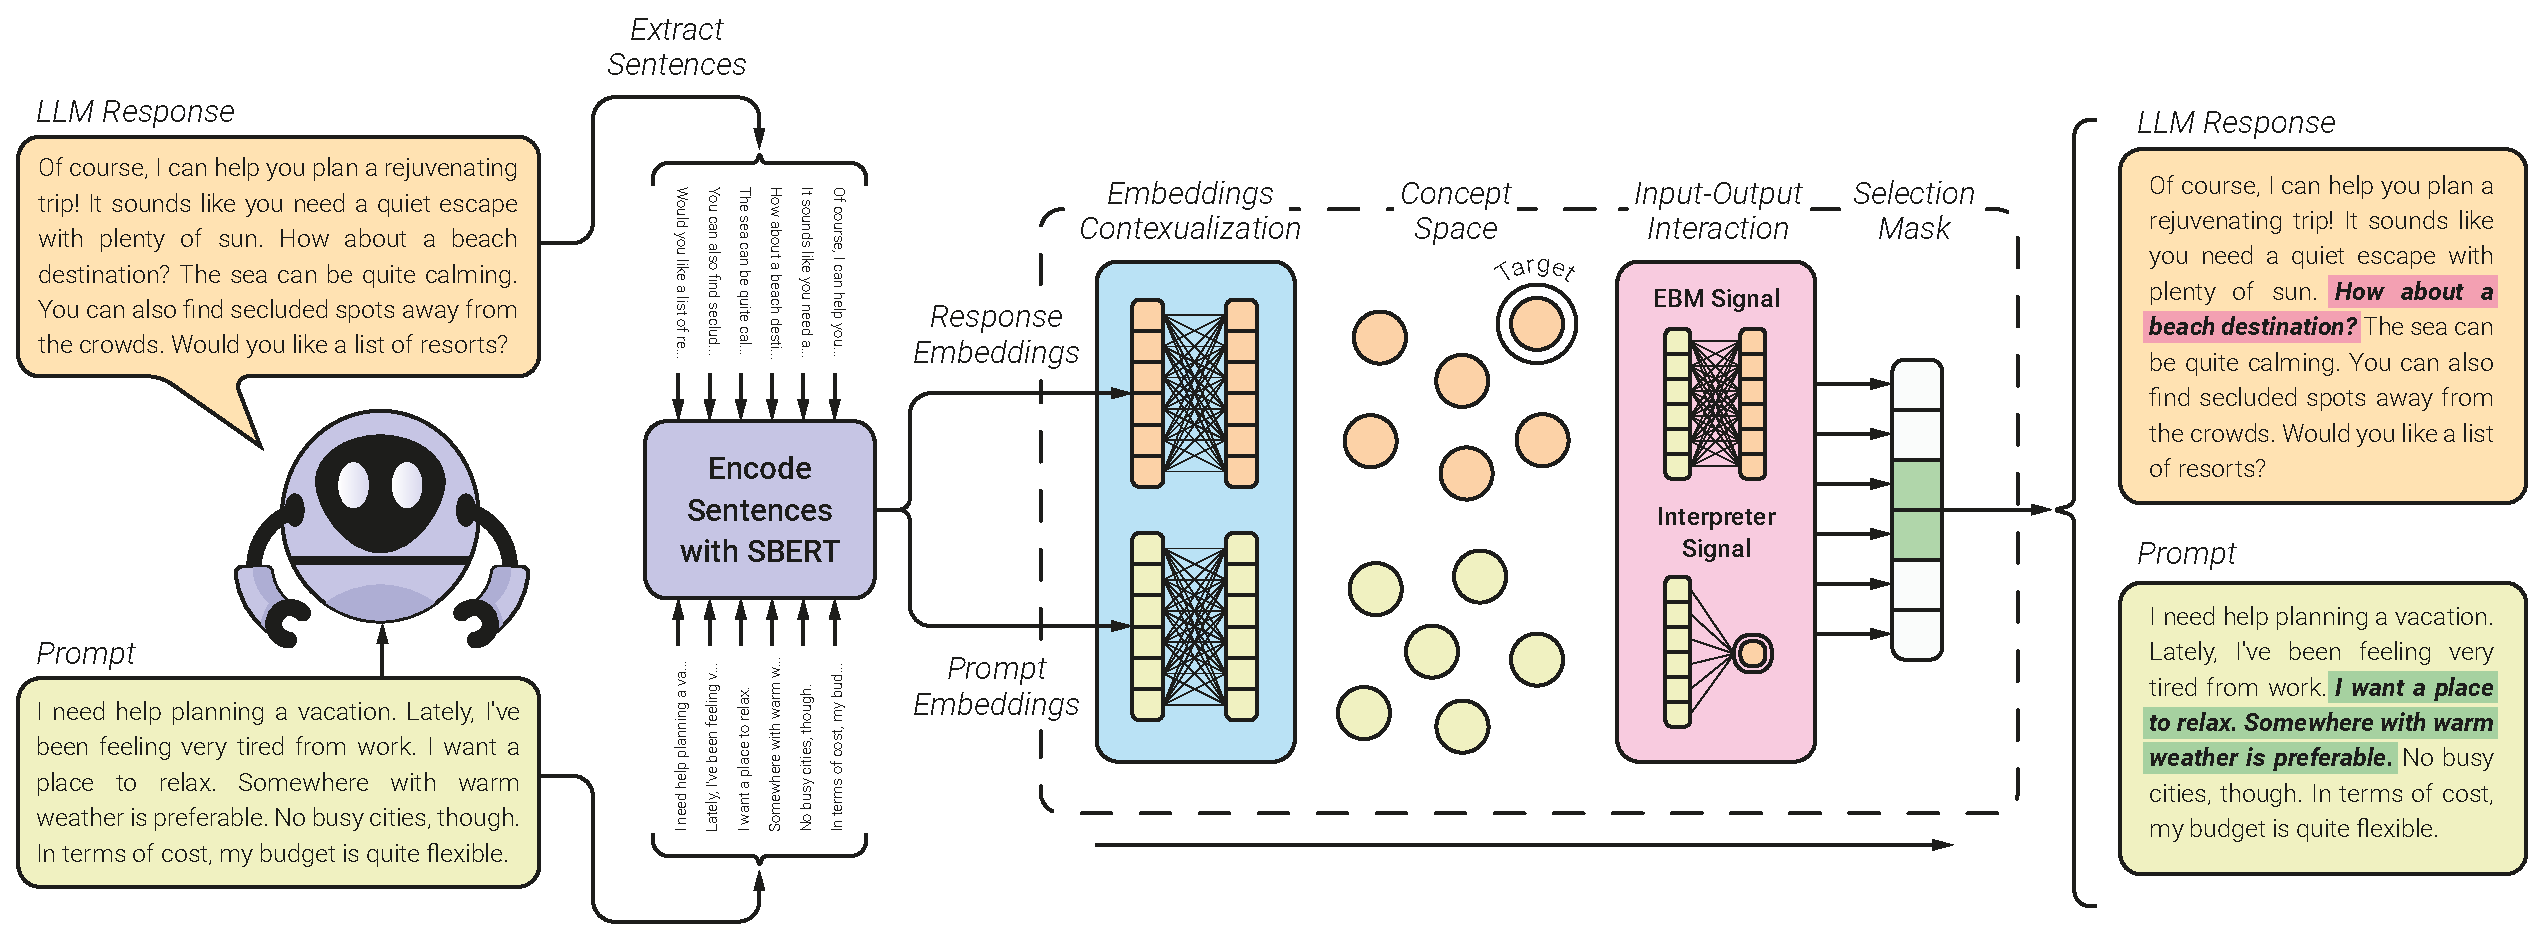
\includegraphics[width=\textwidth]{figures/Fig-Framework-Overview-V5.pdf}
    \caption{نمای کلی چارچوب پیشنهادی (\lr{ESCI})}\label{fig:chap4_framework_overview}
\end{figure}

همان‌طور که در شکل~\ref{fig:chap4_framework_overview} مشاهده می‌شود، روند اجرای این خط‌لوله از چپ به راست طی می‌شود. برای یک جفت (پرامپت، پاسخ) داده‌شده از مدل زبانی جعبه‌سیاه، ابتدا متن به جملات مجزا شکسته شده و توسط یک مدل پیش‌آموزش‌دیده مانند \lr{Sentence-BERT} به بردارهای تعبیه تبدیل می‌شود. سپس، ماژول‌های تصویرساز این تعبیه‌ها را زمینه‌سازی کرده و آن‌ها را به یک فضای مفهومی مشترک نگاشت می‌کنند؛ فضایی که در آن مجاورت هندسی بردارها نشان‌دهنده‌ی ارتباطات متنی جملات است. پس از تعیین شاخص‌های هدف خروجی ($T$)، ماژول تعاملی میزان انطباق‌پذیری ساختاری میان مفاهیم ورودی و خروجی را ارزیابی می‌کند. این ماژول‌ها با بهره‌گیری از سیگنال‌های دریافتی از یک شبکه‌ی انرژی که میزان انطباق‌پذیری ساختاری و معنایی میان ورودی و خروجی را بر اساس الگوهای متنی مدل هدف ارزیابی می‌کند، هدایت می‌شوند. شبکه‌ی مفسر با دریافت پرامپت کامل، خروجی کامل و شاخص‌های هدف خروجی، ماسک اهمیتی تولید می‌نماید که پیش‌آیندهای اثرگذار ورودی را برای گزاره‌های هدف خروجی مشخص می‌سازد. در نهایت، همان‌طور که در سمت راست تصویر نمایان است، با اعمال این ماسک، جملات پیش‌آیند منتخب ورودی استخراج می‌شوند.

شایان ذکر است که این شکل تنها یک نمای کلی از فرایند را نشان می‌دهد و فازهای مجزا را به‌تفکیک در بر ندارد. به‌منظور تحقق این فرایند، به‌جای جستجوی پرهزینه در فضای خروجی مدل هدف، معماری \lr{ESCI} بر اساس دو فاز درهم‌تنیده بنا شده است که در ادامه‌ی این فصل با جزئیات بررسی خواهند شد:

\begin{enumerate}
    \item \textbf{فاز اول (مدل جانشین مبتنی بر انرژی):} در این فاز، یک مدل مبتنی بر انرژی (\lr{EBM}) با معماری ترنسفورمر دوسویه ($\mathcal{E}_{\text{\lr{LM}}}(\mathbf{x}, \mathbf{y}; \theta)$) به‌عنوان مدل جانشین آموزش می‌بیند تا میزان انطباق‌پذیری ساختاری و معنایی میان پرامپت ورودی و پاسخ تولیدشده را بر مبنای الگوهای متنیِ مشاهده‌پذیر ارزیابی کند. دلیل انتخاب \lr{EBM} این است که فرایند انتساب نیازمند ارزیابی انطباق‌پذیری در سطح توالی کامل است؛ ساختاری که بدون وابستگی به نرمال‌سازی محاسبه‌ناپذیر احتمالات روی فضای نمایی خروجی‌ها و بدون نیاز به لوجیت‌ها یا فعال‌سازی‌های درونی، میزان همخوانی پرامپت و پاسخ را در قالب یک تابع انطباق‌پذیریِ نرمال‌نشده ارزیابی می‌نماید. این شبکه یک تابع انرژی اسکالر می‌آموزد که سطوح پایین‌تر آن بازتاب‌دهنده‌ی انطباق‌پذیری بالاتر بر اساس مشاهدات متنی است.
    
    \item \textbf{فاز دوم (شبکه‌ی مفسر هدایت‌شده):} در فاز عملیاتی، یک شبکه‌ی مفسر مستقل ($\mathcal{IN}(\mathbf{x}, \mathbf{y}, T; \alpha)$) با معماری ترنسفورمر دوسویه، برای تولید بردار ماسک اهمیت ($\mathbf{m}$) طراحی شده است. این مفسر پرامپت کامل ($\mathbf{x}$)، پاسخ کامل تولیدشده ($\mathbf{y}$) و مجموعه‌ی شاخص‌های هدف خروجی ($T$) را دریافت کرده و با شرطی‌سازی بازنمایی‌های خروجی بر روی شاخص‌های هدف و بهره‌گیری از سیگنال‌های دریافتی از چشم‌انداز انرژی مدل جانشین، یاد می‌گیرد که اثرگذارترین پیش‌آیندهای پرامپت را شناسایی و استخراج نماید. پس از اتمام آموزش، شبکه‌ی مفسر به‌صورت مستقل و در زمان‌ثابت برای انتساب نمونه‌های جدید به‌کار گرفته می‌شود.
\end{enumerate}

طراحی این رویکرد دوفازی مفسر را قادر می‌سازد تا تنها با یک بار عبور پیش‌رو در گراف محاسباتی خود و بدون نیاز به استعلام مجدد از مدل جعبه‌سیاه در زمان استنتاج، پیش‌آیندهای اثرگذار را استخراج نماید. در بخش‌های بعدی، مراحل پیش‌پردازش، معماری دقیق لایه‌ها و الگوریتم‌های بهینه‌سازی توأم در هر یک از این دو فاز به‌تفصیل فرمول‌بندی خواهند شد.



\section{پیش‌پردازش و استخراج ویژگی‌ها}\label{sec:4-2}

پردازش متون طبیعی توسط معماری‌های عصبی پیشرفته، نیازمند گذار از فضای نمادین و گسسته‌ی کلمات به یک فضای برداری پیوسته و محاسبه‌پذیر است. از آنجا که چارچوب پیشنهادی ما (\lr{ESCI}) واحد تحلیل خود را بر مبنای مفاهیم گزاره‌ای (جملات) استوار کرده است، خط‌لوله‌ی ورود داده‌ها به مدل باید به‌گونه‌ای طراحی شود که علاوه بر استخراج دقیق این واحدهای معنایی، آن‌ها را در قالب ماتریس‌هایی با ابعاد ثابت و منطبق با مکانیزم‌های توجهِ ترنسفورمرها آماده‌سازی کند.

این فرایند در سه گام اساسی تقطیع، تعبیه‌سازی، و نرمال‌سازی ابعاد انجام می‌پذیرد.


\subsection{تقطیع جملات}\label{sec:4-2-1}

نخستین گام در آماده‌سازی داده‌ها، شکستن متن خام ورودی (پرامپت کاربر) و خروجی (پاسخ مدل زبانی) به دنباله‌ای از گزاره‌ها یا به‌طور دقیق‌تر جملات است. برای انجام این تقطیع، از کتابخانه‌ی پردازش زبان طبیعی \lr{spaCy}~\cite{honnibal2017spacy} استفاده می‌شود. این ابزار که توسط شرکت \lr{Explosion AI} توسعه یافته است، یک کتابخانه‌ی متن‌باز و صنعتی است که برخلاف ابزارهای سنتی‌تر (مانند \lr{NLTK}~\cite{loper2002nltk} که بیشتر با اهداف آموزشی و مبتنی بر روش‌های آماری ساده‌تر طراحی شده‌اند)، مشخصاً برای پیاده‌سازی‌های سریع و کاربردهای عملیاتی در مقیاس بزرگ بهینه‌سازی شده است.

مزیت اصلی \lr{spaCy} در تقطیع جملات، اتکای آن به تجزیه‌گر وابستگی نحوی است. در حالی که روش‌های کلاسیک اغلب به علائم نگارشی (مانند نقطه یا علامت سؤال) یا عبارات منظم\enfootnote{regex} وابسته‌اند و در مواجهه با متن‌های بدون ساختار، اختصارات، یا خروجی‌های نامنظم مدل‌های زبانی دچار خطای مرزبندی می‌شوند، \lr{spaCy} با ساخت یک درخت نحوی از کلمات، مرز جملات را بر اساس ساختار دستوری و روابط وابستگی میان توکن‌ها شناسایی می‌کند. این رویکرد به سیستم اجازه می‌دهد تا حتی در متون پیچیده و فاقد علائم نگارشی استاندارد نیز با دقت بالایی عمل کند.

با اعمال این تقطیع، پرامپت خام $\mathbf{x}$ به دنباله‌ای از $N$ جمله‌ی مجزا ($x_1, x_2, \dots, x_N$) و پاسخ خام $\mathbf{y}$ به دنباله‌ای از $M$ جمله‌ی مجزا ($y_1, y_2, \dots, y_M$) تبدیل می‌شوند. این عملیات تضمین می‌کند که بلوک‌های سازنده‌ی تحلیل ما، قطعات تکه‌تکه‌شده‌ی گرامری نبوده و واحدهایی حامل یک فکر یا ایده‌ی کامل باشند که از منظر منطقی و معنایی قابل‌ارزیابی‌اند.


\subsection{تولید تعبیه‌ها}\label{sec:4-2-2}

پس از استخراج جملات، هر جمله‌ی گسسته باید به یک بردار متراکم در فضایی پیوسته نگاشت شود تا ماشین قادر به درک ویژگی‌های معنایی آن باشد. برای تحقق این امر، از ماژول پیش‌آموزش‌دیده‌ی \lr{Sentence-BERT}~\cite{reimers2019sentencebert} استفاده می‌کنیم. همان‌گونه که در بخش~\ref{sec:2-3-4} تشریح شد، این معماری سیامی آموزش دیده است تا جملاتی را که از نظر معنایی مشابه‌اند، به بردارهایی با فاصله‌ی هندسی نزدیک به هم نگاشت کند. لازم به ذکر است که این نزدیکی صرفاً سطحی بوده و مدل برای تولید تعبیه‌های جملات به‌صورت مستقل عمل می‌کند؛ لذا تعبیه‌های حاصل از این مرحله، میان جملات مستقل هستند و اطلاعاتی از هم برای درک بهتر بستر کل متن ندارند. به‌عبارتی، می‌توان گفت تعبیه‌های حاصل برای هر جمله مانند تعبیه‌های حاصل برای هر توکن در خط‌لوله‌ی ترنسفورمر پیش از ورود به معماری اصلی هستند.

در اجرای این چارچوب (برای مثال با بهره‌گیری از مدل \texttt{all-mpnet-base-v2}~\cite{song2020mpnet})، وزن‌های شبکه‌ی تعبیه‌ساز به‌طور کامل منجمد نگه‌داشته می‌شوند تا ویژگی‌های معنایی ایستا و ارگانیک جملات بدون دست‌خوردگی حفظ شوند. با عبور جملات پرامپت و پاسخ از این ماژول، هر جمله به یک بردار پیوسته با طول $d$ نگاشت می‌گردد. در نتیجه، رشته‌ی جملات پرامپت به یک دنباله از بردارهای تعبیه $S^{\text{\lr{in}}}$ و جملات پاسخ به دنباله‌ای از تعبیه‌های $S^{\text{\lr{out}}}$ تبدیل می‌شوند:
\begin{align}
    S^{\text{\lr{in}}} &= (\mathbf{e}_{x_1}, \mathbf{e}_{x_2}, \dots, \mathbf{e}_{x_N}) \label{eq:chap4_embed_in} \\
    S^{\text{\lr{out}}} &= (\mathbf{e}_{y_1}, \mathbf{e}_{y_2}, \dots, \mathbf{e}_{y_M}) \label{eq:chap4_embed_out}
\end{align}
که در آن هر $\mathbf{e}_i \in \mathbb{R}^d$ نشان‌دهنده‌ی بردار تعبیه‌ی یک جمله است و $d$ (که در پیاده‌سازی ما برابر با ۷۶۸ است) ابعاد فضای تعبیه‌ی \lr{Sentence-BERT} را مشخص می‌کند. این دنباله‌ها، نقشی مشابه با تعبیه‌ی توکن‌ها را برای معماری ترنسفورمری دوسویه‌ی ما ایفا می‌کنند، با این تفاوت که هر عضو دنباله، بار معنایی یک جمله‌ی کامل را در خود جای داده است.


\subsection{نرمال‌سازی و پدینگ}\label{sec:4-2-3}

شبکه‌های عصبی عمیق، به‌ویژه بلوک‌های مجهز به مکانیزم توجه با ابعاد ثابت، برای پردازش موازی دسته‌ای داده‌ها نیازمند دریافت ماتریس‌هایی با ابعاد کاملاً یکسان هستند. از آنجا که تعداد جملات در پرامپت‌ها ($N$) و پاسخ‌ها ($M$) در واقعیت همواره متغیر است، ما از یک استراتژی پدینگ اختصاصی بهره می‌بریم.

بدین‌منظور، یک ابرپارامتر وابسته به وظیفه تحت عنوان حداکثر طول دنباله یا $N_{\text{\lr{max}}}$ تعریف می‌شود. برای تعیین این ابرپارامتر، تحلیلی بر توزیع آماری تعداد جملات در وظیفه‌ی مورد نظر صورت گرفته و بنا به ملاحظات ساختاری، اندازه‌ی بیشینه‌ی مناسب تعیین می‌گردد. پس از تعیین این مقدار، عملیات نرمال‌سازی به رویه‌ی تشریح‌شده انجام می‌شود.

اگر تعداد جملات یک متن (مثلاً $N$) بیشتر از $N_{\text{\lr{max}}}$ باشد، دنباله تا رسیدن به این سقف مجاز بُرش می‌خورد و بخش‌های مازاد حذف می‌شوند. در مقابل، اگر متن کوتاه‌تر از $N_{\text{\lr{max}}}$ باشد، فضاهای خالی در انتهای دنباله با استفاده از تعبیه‌های قابل‌یادگیری به‌عنوان پدینگ پر می‌شوند. برخلاف پدینگ سنتی با بردار صفر، استفاده از بردارهای جای‌نگه‌دار با وزن‌های قابل‌یادگیری به مدل جانشین انرژی اجازه می‌دهد تا در فاز آموزش، رفتار مناسبی را برای نادیده گرفتن این بخش‌های خالی بیاموزد و محاسبات مکانیزم توجه را دچار سوگیری نکند. لازم به ذکر است که ماسک‌گذاری پدینگ نیز طبق اصول معماری ترنسفورمر در این معماری فعال بوده و پدینگ‌ها اثر مستقیم بر محاسبات ندارند.

با اعمال این مرحله‌ی نرمال‌سازی ابعادی، دنباله‌های متغیر ورودی به ماتریس‌هایی با ابعاد ثابت و پایدار تبدیل می‌شوند:
\begin{equation}\label{eq:chap4_final_tensors}
    S^{\text{\lr{in}}}, S^{\text{\lr{out}}} \in \mathbb{R}^{N_{\text{\lr{max}}} \times d}
\end{equation}
این ماتریس‌های دوبعدی، به‌عنوان ورودی‌های استاندارد، آماده‌ی تغذیه به فاز اول سیستم (جهت تصویرسازی به فضای مفهومی و محاسبه‌ی انرژی) و فاز دوم (جهت استخراج ماسک‌های اهمیت پیش‌آیند) می‌باشند.



\section{فاز اول: مدل جانشین مبتنی بر انرژی}\label{sec:4-3}

همان‌گونه که در تشریح نمای کلی چارچوب بیان شد، هسته‌ی محاسباتی \lr{ESCI} بر آموزش یک مدل جانشین استوار است. اتخاذ این استراتژی، پیش از هر چیز، پاسخی عملی به محدودیت‌ها و بن‌بست‌های محاسباتی در روش‌های اختلالیِ زمان استنتاج است. همان‌طور که در فصل پیشین و در بررسی رویکردهایی نظیر \lr{L2X}~\cite{chen2018learning} و \lr{SOInter}~\cite{seyyedsalehi2024sointer} واکاوی شد، ارزیابی انتساب از طریق تقریب‌های نقطه‌ای و جستجوهای محلی برای هر ورودی جدید، علاوه بر تحمیل بار محاسباتی نمایی، غالباً به استخراج سیگنال‌هایی پرنویز و ناپایدار می‌انجامد. در این راستا، پژوهش‌هایی نظیر چارچوب \lr{SILVER}~\cite{li2025fromexplainability} نشان داده‌اند که تجمیع الگوهای رفتاری یک سیستم در قالب آموزش سراسری یک مدل جانشین، رویکردی مستحکم‌تر و پایدارتر برای تقریب رفتار یک سیستم جعبه‌سیاه ارائه می‌دهد. از این رو، فاز نخست چارچوب ما به طراحی مدلی اختصاص دارد که الگوهای انطباق‌پذیری ساختاری و معنایی میان پرامپت و پاسخ را به‌صورت سراسری بر مبنای متون تولیدشده توسط مدل هدف مدل‌سازی نماید.

پرسش بعدی در این معماری، تعیین ساختار این مدل جانشین است. اگرچه رویکردهایی نظیر \lr{TriSum}~\cite{jiang2024trisum} تلاش کرده‌اند با استفاده از تقطیر دانش، جانشین‌های زایایی بسازند که توجیهات متنی و روند استنتاج را مستقیماً تولید کنند، اما این رهیافت با چالش‌های نظری عمیقی همراه است. وادار کردن یک شبکه‌ی ثانویه به تولید زبان طبیعی، بار پردازش قواعد نحوی، گرامر و دینامیک‌های پیچیده‌ی خودهمبسته را به آن تحمیل می‌کند. این پیچیدگی ساختاری به‌طور اجتناب‌ناپذیری باعث می‌شود تا مدل جانشین درگیر داستان‌پردازی و خطاهای زبانی خود گردد؛ پدیده‌ای که در نهایت به بروز توهم تفسیرپذیری~\cite{friedman2024interpretability} در مواجهه با داده‌های خارج از توزیع (\lr{OOD}) منجر می‌شود. برای پرهیز از این نارسایی‌ها، مدل جانشین ما اساساً برای تولید متن طراحی نشده است؛ بلکه نقش آن به یک ارزیاب ساختاریافته تقلیل یافته است تا تمام ظرفیت پارامتری خود را منحصراً به مدل‌سازی انطباق‌پذیری و روابط میان جملات اختصاص دهد.

برای ایفای نقش این ارزیاب کلان‌نگر، انتخاب یک \lr{EBM} در برابر مدل‌های احتمالی استاندارد یا یک دسته‌بند ساده، تصمیمی مبتنی بر مبانی یادگیری آماری است. بر اساس مبانی نظری لکان و همکاران (۲۰۰۶)~\cite{lecun2006tutorial}، یک مدل احتمالی استاندارد برای ارزیابی متغیرها نیازمند محاسبه‌ی تابع افراز و نرمال‌سازی احتمالات بر روی تمامی خروجی‌های ممکن است؛ محاسبه‌ای که در فضای بی‌کران و نامتناهی زبان از نظر ریاضی غیرقابل‌حل است. از سوی دیگر، دسته‌بندهای ساده فاقد ظرفیت لازم برای مدل‌سازی ساختارهای درهم‌تنیده‌ی متوالی هستند و مدل‌های خودهمبسته نیز متن را صرفاً به‌صورت مقطعی و کلمه‌به‌کلمه ارزیابی می‌کنند. یک \lr{EBM} با دور زدن نیاز به نرمال‌سازی احتمالات، به‌عنوان یک تابع انطباق‌پذیریِ نرمال‌نشده عمل کرده و می‌تواند با نگاهی کل‌نگر، ساختار کلان پرامپت و پاسخ را به‌صورت یکپارچه ارزیابی نماید~\cite{bakhtin2019realfake, deng2020residual, bakhtin2021residual, bhattacharyya2021reranking, qin2022cold, xu2025energybased}. علاوه بر این، شواهد در ادبیات تقطیر دانش~\cite{gu2021fully} نشان می‌دهد که معماری‌های عصبی ظرفیت بالایی در یادگیری الگوهای توالی از یک مدل معلم دارند؛ قابلیتی که به ما اجازه می‌دهد چشم‌انداز انرژی را صرفاً بر روی خروجی‌های مدل جعبه‌سیاه تنظیم کنیم و وابستگی‌های متنی را در قالب یک مقدار اسکالر (انرژی) استخراج نماییم.

در نهایت، تمرکز انحصاری این مدل انرژی بر روی متون خروجی نهایی (جملات تولیدشده) و عدم‌اتکا به لایه‌های پنهان مدل اصلی، یک انتخاب عمل‌گرایانه برای برخورد با جعبه‌سیاه‌های مسدود است که از نظر تئوریک نیز توجیه می‌پذیرد. همان‌گونه که جین و همکاران (۲۰۲۵)~\cite{jin2025exploring} با معرفی سنجه‌ی عمق مفهوم نشان دادند، فرایند شکل‌گیری مفاهیم در ترنسفورمرها به‌شدت سلسله‌مراتبی است و مفاهیم انتزاعی و پیچیده غالباً در عمیق‌ترین لایه‌های انتهایی شبکه به بلوغ می‌رسند. در نتیجه، ردیابی لایه‌به‌لایه‌ی این مفاهیمِ در حال تکامل، مستعد استخراج سیگنال‌هایی پرنویز است. از این رو، ارزیابی کل‌نگر جملاتِ تکامل‌یافته توسط \lr{EBM}، نشانگرهایی پایدار و عینی از نحوه‌ی اثرگذاری ورودی بر پاسخ بر مبنای متون مشاهده‌پذیر فراهم می‌سازد، بدون آنکه متکی بر فرضیات اثبات‌نشده پیرامون پویایی بازنمایی‌های درونی مدل باشد.

بر پایه‌ی این توجیهات نظری، در ادامه‌ی این بخش ابتدا به تشریح جزئیات معماری این شبکه‌ی انرژی پرداخته و سپس استراتژی‌های نمونه‌برداری تقابلی برای آموزش بدون نیاز به حقیقت پایه‌ی آن را فرمول‌بندی خواهیم کرد.


\subsection{معماری شبکه‌ی انرژی}\label{sec:4-3-1}

هدف اصلی شبکه‌ی انرژی در چارچوب ما ($\mathcal{E}_{\text{\lr{LM}}}(\mathbf{x}, \mathbf{y}; \theta)$)، یادگیری چشم‌انداز انرژی برای یک جفت پرامپت و پاسخ داده‌شده است. این شبکه آموزش می‌بیند تا با ارزیابی این جفت، انرژی پایین‌تری به تعاملات و وابستگی‌هایی تخصیص دهد که با الگوهای متنیِ مشاهده‌شده در خروجی‌های مدل هدف منطبق‌ترند. همان‌طور که در شکل~\ref{fig:chap4_architecture_energy} نشان داده شده است، این معماری یک شبکه‌ی ترنسفورمری تطبیق‌یافته است که از چندین بلوک محاسباتی متوالی تشکیل شده تا ماتریس‌های تعبیه‌ی ورودی ($S^{\text{\lr{in}}}$) و خروجی ($S^{\text{\lr{out}}}$) را در نهایت به یک انرژی اسکالر تبدیل کند. شایان ذکر است که در این معماری، ترنسفورمر به‌صورت دوسویه عمل می‌کند؛ بدین‌معنا که برخلاف مدل‌های خودهمبسته، هیچ‌گونه ماسک توجه برای جلوگیری از نگاه به آینده در جریان محاسبات آن اعمال نمی‌شود و شبکه در هر لایه، تمام توالی را به‌طور یکپارچه ارزیابی می‌کند.

\begin{figure}[ht]
    \centering
    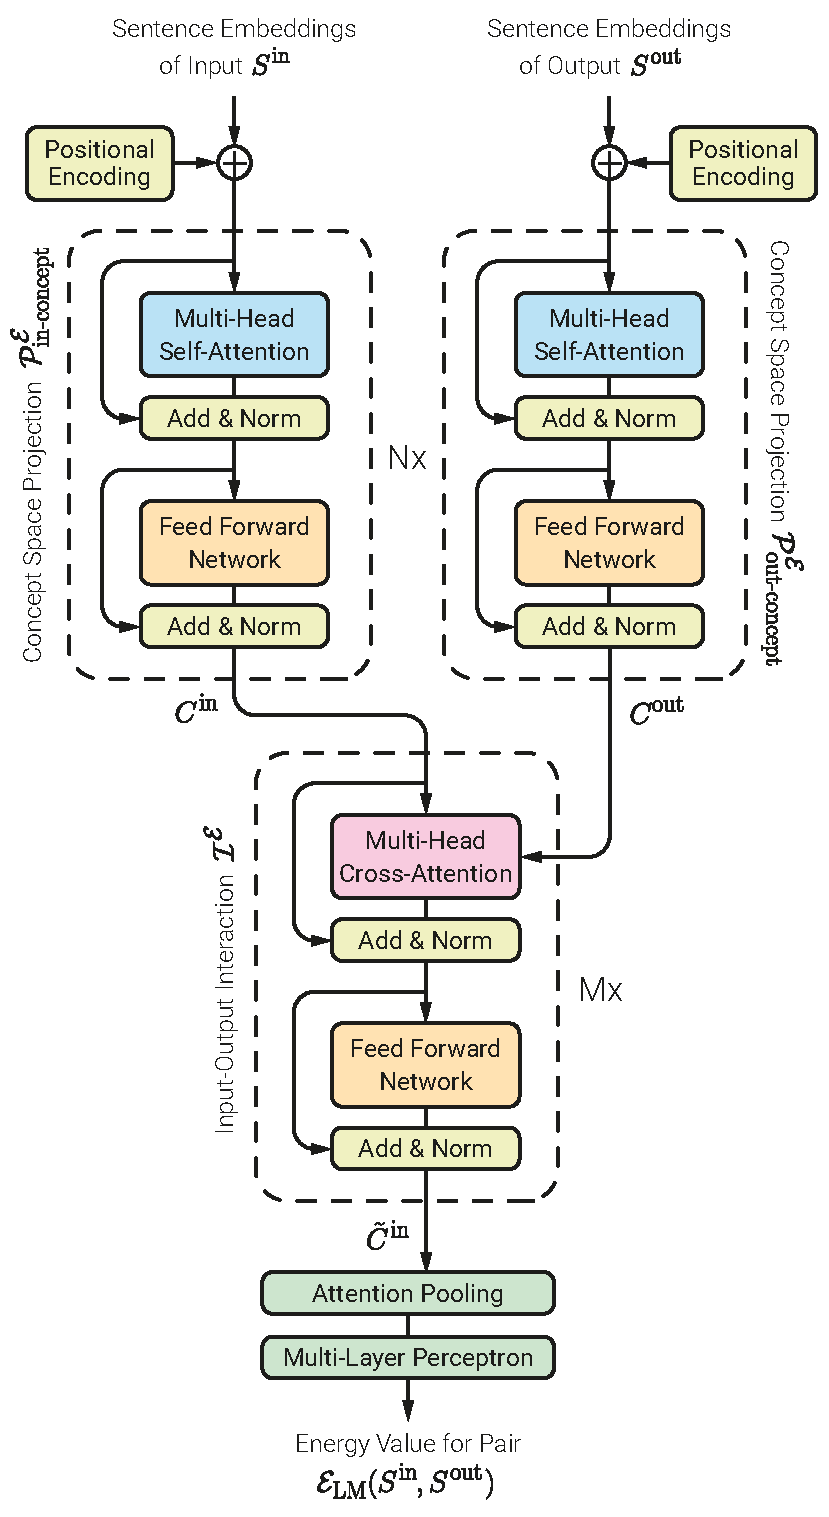
\includegraphics[width=0.45\textwidth]{figures/Fig-EBM-Architecture-V4.pdf}
    \caption{معماری شبکه‌ی جانشین مبتنی بر انرژی ($\mathcal{E}_{\text{\lr{LM}}}$)}\label{fig:chap4_architecture_energy}
\end{figure}

پیش از ورود به ماژول‌های اصلی، از آنجا که مدل‌سازی ما در سطح جملات انجام می‌شود و ترتیب گزاره‌ها در درک بافتار متن نقشی اساسی ایفا می‌کند، ابتدا مانند ترنسفورمر استاندارد طبق بخش~\ref{sec:2-2} یک لایه‌ی رمزگذاری موقعیتی به ماتریس‌های خام افزوده می‌گردد تا اطلاعات ترتیبی حفظ شود:
\begin{align}
    \tilde{S}^{\text{\lr{in}}} &= S^{\text{\lr{in}}} + E_{\text{\lr{pos}}}^{\text{\lr{in}}} \label{eq:chap4_pos_enc_in} \\
    \tilde{S}^{\text{\lr{out}}} &= S^{\text{\lr{out}}} + E_{\text{\lr{pos}}}^{\text{\lr{out}}} \label{eq:chap4_pos_enc_out}
\end{align}
پس از این گام آماده‌سازی، جریان محاسبات در سه مرحله‌ی تصویرسازی فضای مفهومی، تعامل ورودی-خروجی و محاسبه‌ی انرژی انجام می‌شود.

\paragraph{۱. تصویرسازی فضای مفهومی.}
در گام نخست، تانسورهای ورودی ($\tilde{S}^{\text{\lr{in}}}$ و $\tilde{S}^{\text{\lr{out}}}$) به‌عنوان ورودی به دو ماژول خودتوجهی مجزا، یعنی $\mathcal{P}_{\text{\lr{in-concept}}}^{\mathcal{E}}$ و $\mathcal{P}_{\text{\lr{out-concept}}}^{\mathcal{E}}$ تغذیه می‌شوند. دلیل تعبیه‌ی این مرحله‌ی میانی، محدودیت‌های بازنمایی ایستا در غیاب بافتار است.

پژوهش‌های انجام‌شده در مدل‌های مفهومی بزرگ~\cite{lcmteam2024lcm} نشان داده‌اند که مدل‌سازی روابط معنایی می‌تواند با دقت مناسب در فضای پیوسته‌ی تعبیه‌های جمله‌ای انجام پذیرد و نیازی به درگیری با فرم خرد توکن‌ها نیست. همان‌طور که در پژوهش خطیر و همکاران (۲۰۲۵)~\cite{khatir2025aligned} تبیین شد، تعبیه‌های ایستا (مانند خروجی شبکه‌ای نظیر \lr{Sentence-BERT}) از همان ابتدا دارای یک ساختار گروه‌بندی غنی هستند و هم‌تراز در مبدأ محسوب می‌شوند. این ویژگی به ما اجازه می‌دهد تا از این بردارها به‌عنوان یک نقطه‌ی شروع قابل‌اتکا استفاده کنیم. با این وجود، تعبیه‌های ایستا مفاهیم را صرفاً در انزوا مدل می‌کنند. همان‌گونه که پارک و همکاران (۲۰۲۴)~\cite{park2024emergence} در تحلیل دینامیک مفاهیم نشان دادند، مفاهیم در بستر یک بافتار مشخص به‌صورت پویا با یکدیگر تعامل دارند و این فضای مفهومی، دارای وابستگی‌هایی است که فراتر از شباهت معنایی خام هستند.

ماژول‌های تصویرساز فضای مفهومی با در نظر گرفتن این ظرایف طراحی شده‌اند. هر یک از این دو ماژول، شامل $N$ لایه از بلوک‌های استاندارد رمزگذار ترنسفورمر (شامل مکانیزم توجه چندسره و شبکه‌های پیش‌خور همراه با اتصالات باقیمانده و نرمال‌سازی لایه‌ای) هستند. این ماژول‌ها مفاهیم ایستای اولیه را دریافت کرده و با استفاده از مکانیزم خودتوجهی، به جملات اجازه می‌دهند تا برای درک دقیق‌تر معنای خود، به سایر جملات موجود در همان پرامپت (یا پاسخ) توجه کنند. این فرایند زمینه‌سازی بافتاری، بازنمایی هر گزاره را پیش از ارزیابی تعامل متقاطع غنی‌سازی می‌کند و در نتیجه، تعبیه‌های اولیه را به یک فضای مفهومی پویا نگاشت می‌نماید:
\begin{align}
    C^{\text{\lr{in}}} &= \mathcal{P}_{\text{\lr{in-concept}}}^{\mathcal{E}}(\tilde{S}^{\text{\lr{in}}}) \label{eq:chap4_concept_in} \\
    C^{\text{\lr{out}}} &= \mathcal{P}_{\text{\lr{out-concept}}}^{\mathcal{E}}(\tilde{S}^{\text{\lr{out}}}) \label{eq:chap4_concept_out}
\end{align}

\paragraph{۲. تعامل ورودی-خروجی.}
پس از آنکه مفاهیم ورودی و خروجی در بافتار مستقل خود زمینه‌سازی شدند، ضرورت دارد تا میزان انطباق‌پذیری ساختاری و معنایی میان پرامپت و پاسخ ارزیابی شود. در این مرحله، از یک ماژول تعاملی ($\mathcal{I}^{\mathcal{E}}$) مبتنی بر توجه متقاطع استفاده می‌گردد. طراحی این بلوک بر پایه‌ی یافته‌های باتاچاریا و همکاران (۲۰۲۱)~\cite{bhattacharyya2021reranking} استوار است؛ آن‌ها در ارزیابی مدل‌های رتبه‌بندی انرژی نشان دادند که مدل‌هایی که انرژی را صرفاً بر اساس بررسی جمله‌ی خروجی در انزوا محاسبه می‌کنند (مدل‌های انرژی حاشیه‌ای)، در ارزیابی وابستگی‌ها با افت عملکرد مواجه می‌شوند؛ در حالی که مدل‌های انرژی مشترک\enfootnote{joint energy models} که ترکیب ورودی و خروجی را به‌طور هم‌زمان داوری می‌کنند، دقت بسیار بالاتری دارند.

ماژول تعامل ورودی-خروجی ما، که از $M$ لایه از بلوک‌های توجه متقاطع تشکیل شده است، پیاده‌سازی همین ارزیابی مشترک است. هر یک از این لایه‌ها علاوه بر مکانیزم توجه، مجهز به شبکه‌های پیش‌خور، اتصالات باقیمانده و لایه‌های نرمال‌سازی هستند. مطابق با جریان اطلاعات در شکل~\ref{fig:chap4_architecture_energy}، در این ماژول، مفاهیم پویای پرامپت ($C^{\text{\lr{in}}}$) در نقش بردارهای پرسمان ($Q$)، و مفاهیم پویای پاسخ ($C^{\text{\lr{out}}}$) در نقش بردارهای کلید ($K$) و ارزش ($V$) عمل می‌کنند. این مکانیزم به مفاهیم ورودی اجازه می‌دهد تا با مفاهیم خروجی تعامل کرده و بررسی کنند که گزاره‌های پرامپت تا چه میزان با پاسخ تولیدشده انطباق دارند. خروجی این بلوک، نسخه‌ی به‌روزرسانی‌شده‌ای از بازنمایی پرامپت است که آگاهی کاملی از تعاملات خود با پاسخ مدل دارد:
\begin{equation}\label{eq:chap4_cross_attention_interaction}
    \tilde{C}^{\text{\lr{in}}} = \mathcal{I}^{\mathcal{E}}\big(Q=C^{\text{\lr{in}}}, K=C^{\text{\lr{out}}}, V=C^{\text{\lr{out}}}\big)
\end{equation}

\paragraph{۳. محاسبه‌ی انرژی.}
در گام نهایی، اطلاعات تعاملی توزیع‌شده در ماتریس $\tilde{C}^{\text{\lr{in}}}$ باید در قالب یک امتیاز اسکالر یکپارچه شود. معماری این بخش از متمایزگر ترنسفورمری در چارچوب \lr{EBM} بختیین و همکاران (۲۰۱۹)~\cite{bakhtin2019realfake} الهام گرفته شده است، با این تفاوت که با خروجی‌های ساختاریافته‌ی بلوک‌های پیشین تغذیه می‌شود.

از آنجا که هدف ما استخراج یک عدد منفرد (اسکالر انرژی) است، نیازمند عبور داده‌ها از یک شبکه‌ی عصبی پیش‌خور (\lr{MLP}) هستیم. با این وجود، خروجی بلوک تعاملی یک ماتریس دوبعدی از تعبیه‌های متنی با ابعاد $N_{\text{\lr{max}}} \times d$ است. برای فشرده‌سازی اصولی اطلاعات در طول بُعد دنباله بدون از دست دادن وزن متغیر جملات، از یک لایه‌ی تجمیع مبتنی بر توجه\enfootnote{attention pooling} استفاده می‌شود. این عملگر به مدل اجازه می‌دهد تا برخلاف تجمیع میانگین ساده، وزن بیشتری به جملاتی اختصاص دهد که حامل وابستگی تعاملی و معنایی قوی‌تری در بازنمایی نهایی هستند و در نهایت، ماتریس جملات را به یک بردار متراکم واحد ($\mathbf{h}_{\text{\lr{pool}}} \in \mathbb{R}^d$) تقلیل دهد:
\begin{equation}\label{eq:chap4_attention_pooling}
    \mathbf{h}_{\text{\lr{pool}}} = \text{\lr{AttentionPooling}}(\tilde{C}^{\text{\lr{in}}})
\end{equation}
سپس، این بردار فشرده به یک شبکه‌ی عصبی پیش‌خور تمام‌متصل (\lr{MLP}) تغذیه می‌شود تا ویژگی‌ها به یک عدد منفرد تصویر شوند. این عدد اسکالر نهایی، همان انرژی محاسبه‌شده ($\mathcal{E}_{\text{\lr{LM}}}$) است که نشان می‌دهد با توجه به چشم‌انداز انرژی تقریب‌زده‌شده از مدل جعبه‌سیاه، جفت پرامپت و پاسخ تا چه میزان با یکدیگر انطباق دارند:
\begin{equation}\label{eq:chap4_energy_calc}
    \mathcal{E}_{\text{\lr{LM}}}(\mathbf{x}, \mathbf{y}; \theta) = \text{\lr{MLP}}(\mathbf{h}_{\text{\lr{pool}}})
\end{equation}
با فرمول‌بندی این معماری پیش‌رو، در بخش بعدی به چگونگی آموزش این شبکه و تنظیم وزن‌های $\theta$ از طریق توابع زیان تقابلی خواهیم پرداخت.


\subsection{استراتژی پیش‌آموزش و تابع زیان دوگانه}\label{sec:4-3-2}

پس از طراحی معماری شبکه‌ی انرژی، مهم‌ترین چالش در استقرار این مدل جانشین، بهینه‌سازی و آموزش آن است. همان‌گونه که در بخش~\ref{sec:2-4-2} تبیین شد، آموزش مستقیم مدل‌های مبتنی بر انرژی بر روی فضای گسسته‌ی متنی از طریق کمینه‌سازی زیان درست‌نمایی، به دلیل محاسبه‌ناپذیری تابع افراز در فضاهای نامتناهی با بن‌بست ریاضی مواجه است؛ لذا طراحی تابع زیان و استراتژی نمونه‌برداری مناسب برای شبکه‌های انرژی از اساسی‌ترین بخش‌های استقرار مؤثر آن‌هاست. برای عبور از این محدودیت ساختاری و در هماهنگی با رویکردهای یادگیری انرژی پیرو بخش~\ref{sec:2-4-4}، چارچوب \lr{ESCI} از یادگیری تقابلی بهره می‌برد تا بدون نیاز به مدل‌سازی صریح تمامی خروجی‌های ممکن، چشم‌انداز انرژی را شکل دهد.

در انتخاب نوع تابع زیان تقابلی، ما به یافته‌های دنگ و همکاران (۲۰۲۰)~\cite{deng2020residual} و بختیین و همکاران (۲۰۲۱)~\cite{bakhtin2021residual} استناد کرده‌ایم که نشان دادند استفاده از توابع حاشیه‌ای کلاسیک در فضاهای زبانی غالباً با ناپایداری در آموزش مدل‌های انرژی همراه است. بر این اساس، استفاده از استراتژی‌های مبتنی بر تخمین تقابلی نویز (\lr{NCE})~\cite{gutmann2010noise} راهکاری پایدار برای اجتناب از محاسبه‌ی صریح تابع افراز در پردازش زبان به‌شمار می‌رود.

با این وجود، متدولوژی ما در پیاده‌سازی این رویکرد متمایز از ساختارهای پسماند مرسوم است. در پژوهش‌های دنگ و بختیین، مدل انرژی در قالب یک معماری پسماند و با استفاده از \lr{NCE} دودویی آموزش می‌بیند که در آن توزیع نویز مستقیماً توسط توزیع احتمالات یک مدل زبانی خودهمبسته تأمین می‌گردد. اما در رژیم دسترسی جعبه‌سیاه در چارچوب \lr{ESCI}، ما فاقد دسترسی به توزیع احتمالات و لوجیت‌های مدل هدف هستیم. از این رو، ما از تعمیم چندکلاسه‌ی این رویکرد یعنی \lr{InfoNCE}~\cite{oord2018representation} (که در بخش~\ref{sec:2-4-5} تشریح شد) بهره برده‌ایم. استفاده از \lr{InfoNCE} به ما اجازه می‌دهد تا یک نمونه‌ی مثبت را به‌صورت هم‌زمان در برابر $K$ نمونه‌ی منفی ساختاریافته قرار دهیم و پایداری محاسباتی آموزش را بدون وابستگی به توزیع‌های احتمالی درونی تأمین نماییم.

\begin{figure}[ht]
    \centering
    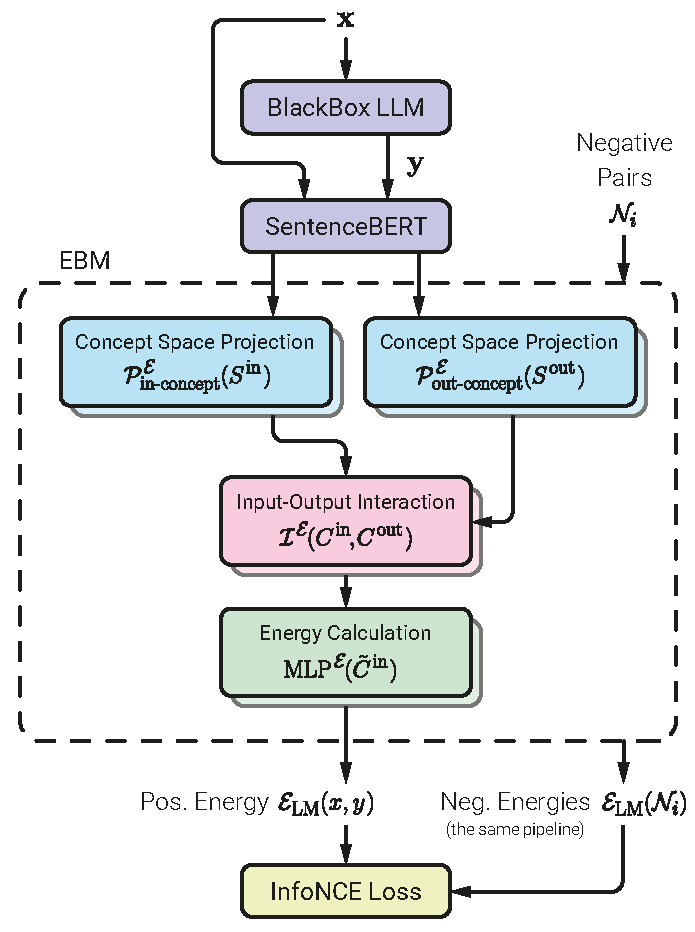
\includegraphics[width=0.5\textwidth]{figures/Fig-EBM-Pretraining-Pipeline-V4.pdf}
    \caption{خط‌لوله‌ی پیش‌آموزش شبکه‌ی جانشین مبتنی بر انرژی ($\mathcal{E}_{\text{\lr{LM}}}$)}\label{fig:chap4_pipeline_energy_pretraining}
\end{figure}

با فرض اینکه جفت منطبق و مثبت ما برای نمونه‌ی $i$ام به‌صورت $(\mathbf{x}_i, \mathbf{y}_i)$ تعریف شود، مجموعه‌ای متشکل از $K$ نمونه‌ی منفی متناظر با همین جفت را به‌صورت $\mathcal{N}_i = \{(\mathbf{x}'_1, \mathbf{y}'_1), \dots, (\mathbf{x}'_K, \mathbf{y}'_K)\}$ در نظر می‌گیریم. برای انسجام، یک تابع امتیازدهی مبتنی بر انرژی به فرم $h(\mathbf{x}, \mathbf{y}) = \exp(-\mathcal{E}_{\text{\lr{LM}}}(\mathbf{x}, \mathbf{y};\theta) / \tau)$ تعریف می‌گردد که در آن $\mathcal{E}_{\text{\lr{LM}}}$ خروجی اسکالر شبکه‌ی انرژی و $\tau > 0$ پارامتر دما است. پارامتر دما به‌عنوان مقیاس‌دهنده‌ی هندسی عمل کرده و حساسیت شبکه به اختلاف میان سطوح انرژی را تنظیم می‌نماید. بر این اساس، تابع زیان تقابلی برای نمونه‌ی $i$ام به‌صورت زیر فرمول‌بندی می‌شود:
\begin{equation}\label{eq:chap4_infonce_base}
    \mathcal{L}_i = -\log \left( \frac{h(\mathbf{x}_i, \mathbf{y}_i)}{h(\mathbf{x}_i, \mathbf{y}_i) + \sum_{(\mathbf{x}', \mathbf{y}') \in \mathcal{N}_i} h(\mathbf{x}', \mathbf{y}')} \right)
\end{equation}
این معادله نشان می‌دهد که مدل با کمینه‌سازی $\mathcal{L}_i$، در تلاش است تا نسبت امتیاز نمونه‌ی مثبت را در برابر مجموع امتیازات تمامی گزینه‌ها بیشینه سازد. برای تعمیم این روند به کل مجموعه‌داده، زیان نهایی برای دسته‌ای به اندازه‌ی $B$ برابر با میانگین زیان‌های انفرادی است:
\begin{equation}\label{eq:chap4_infonce_batch}
    \mathcal{L}_{\text{\lr{batch}}} = \frac{1}{B} \sum_{i=1}^{B} \mathcal{L}_i
\end{equation}

ساختار اجرایی این فرایند بهینه‌سازی در شکل~\ref{fig:chap4_pipeline_energy_pretraining} نشان داده شده است. پرامپت خام ابتدا به مدل زبانی جعبه‌سیاه ارسال شده تا پاسخ واقعی تولید گردد. این جفت، پس از تبدیل به بردار توسط شبکه‌ی تعبیه‌ساز، وارد جریان محاسباتی مدل انرژی شده و در نهایت، انرژی اسکالر دریافت می‌کند. هم‌زمان، مجموعه‌ی نمونه‌های منفی ($\mathcal{N}_i$) نیز از همین خط‌لوله عبور کرده و مقادیر انرژی متناظر را تولید می‌نمایند. در گام نهایی، این مقادیر وارد تابع زیان \lr{InfoNCE} می‌شوند تا انرژی جفت‌های واقعی کاهش و انرژی جفت‌های نامنطبق افزایش یابد.

کیفیت چشم‌انداز انرژی حاصل از این خط‌لوله، وابسته به طراحی مجموعه‌ی منفی ($\mathcal{N}_i$) است. ما برای اینکه شبکه‌ی انرژی بتواند هم‌زمان ویژگی‌های آماری کلان و وابستگی‌های ساختاری گزاره‌ای را بیاموزد، تابع زیان نهایی را به‌صورت یک ساختار دوگانه متشکل از دو هدف مکمل طراحی کرده‌ایم:

\paragraph{۱. زیان وفاداری سراسری ($\mathcal{L}_{\text{\lr{fidelity}}}$).}
هدف از این تابع زیان، وادار کردن شبکه به یادگیری الگوهای سبکی و توزیعی خروجی‌های مدل هدف است؛ به‌گونه‌ای که مدل جانشین بیاموزد خروجی‌های واقعی جعبه‌سیاه را از متون تولیدشده در سایر توزیع‌ها متمایز کند. این بخش از تابع زیان، از معماری \lr{EBM} متمایزگر بختیین و همکاران (۲۰۱۹)~\cite{bakhtin2019realfake} الهام گرفته شده است که نشان دادند یک ترنسفورمر دوسویه می‌تواند با تکیه بر نمونه‌های منفی سراسری (نظیر متون انسانی یا متون حاصل از سایر مدل‌ها)، به ارزیابی توانمند برای سنجش انطباق توزیعی تبدیل شود. 

در این راستا، برای هر نمونه‌ی $i$، دو مجموعه‌ی منفی متمایز در نظر گرفته می‌شود: نخست، پاسخ‌های انسانی از مجموعه‌داده‌ی مرجع ($\mathcal{N}^{\text{\lr{hum}}}_i$)؛ و دوم، پاسخ‌های تولیدشده توسط یک مدل زبانی متفاوت ($\mathcal{N}^{\text{\lr{other}}}_i$). با فرض ثابت بودن پرامپت $\mathbf{x}_i$، مجموعه‌ی کل نمونه‌های منفی وفاداری برابر با $\mathcal{N}^{\text{\lr{fid}}}_i = \mathcal{N}^{\text{\lr{hum}}}_i \cup \mathcal{N}^{\text{\lr{other}}}_i$ است. در نتیجه، تابع زیان وفاداری برای نمونه‌ی $i$ام به‌صورت زیر می‌باشد:
\begin{equation}\label{eq:chap4_loss_fidelity}
    \mathcal{L}_{\text{\lr{fidelity}}}^{(i)} = -\log \left( \frac{h(\mathbf{x}_i, \mathbf{y}_i)}{h(\mathbf{x}_i, \mathbf{y}_i) + \sum_{(\mathbf{x},\mathbf{y}') \in \mathcal{N}^{\text{\lr{fid}}}_i} h(\mathbf{x}, \mathbf{y}')} \right)
\end{equation}
این زیان تضمین می‌کند که چشم‌انداز انرژی در مقیاس کلان، به الگوهای متنی مدل جعبه‌سیاه وفادار بماند و از افت عملکرد در درک فضای سراسری جلوگیری نماید.

\paragraph{۲. زیان وابستگی محلی ($\mathcal{L}_{\text{\lr{dep}}}$).}
اگر شبکه‌ی انرژی صرفاً با زیان وفاداری آموزش ببیند، ممکن است به‌جای کشف ارتباطات محتوایی، به همبستگی‌های سطحی بسنده نماید. برای رفع این نقیصه و وادار کردن مدل به سنجش وابستگی‌های ساختاری میان جملات، زیان وابستگی محلی با استفاده از استراتژی نمونه‌برداری پادواقعی\enfootnote{counterfactual sampling} طراحی شده است.

ایده‌ی کلیدی در این بخش، استفاده از ماسک‌گذاری تصادفی برای ارزیابی جزء‌به‌جزء است. برای سنجش اینکه یک بخش از پاسخ تا چه اندازه به بخش خاصی از پرامپت وابسته است، شبکه‌ی انرژی باید این گزاره‌ها را در شرایطی ارزیابی کند که بخش‌هایی از بافتار متنی حذف شده باشند. به همین منظور، در هر گام پردازش، تعدادی از جملات در پرامپت و پاسخ به‌صورت تصادفی ماسک می‌شوند تا یک پرامپت جزئی ($\mathbf{x}_{\text{\lr{part}}}$) و یک پاسخ جزئی ($\mathbf{y}_{\text{\lr{part}}}$) شکل گیرد.

در دسته‌ای به اندازه‌ی $B$، این هدف آموزشی از دو مکانیزم نمونه‌برداری مستقل بهره می‌برد که هر یک با ساخت مجموعه‌ای از نمونه‌های منفی به اندازه‌ی $K = B-1$ برای نمونه‌ی $i$ام عمل می‌کنند:

نخست، نمونه‌بردار پاسخ جزئی که در آن پرامپت جزئی یک نمونه ($\mathbf{x}_{\text{\lr{part}}, i}$) ثابت نگه‌داشته شده و پاسخ جزئی متناظر با آن ($\mathbf{y}_{\text{\lr{part}}, i}$)، در تقابل با پاسخ‌های جزئی سایر نمونه‌های دسته ($\mathbf{y}'_{\text{\lr{part}}, j}$) قرار می‌گیرد. به‌بیان ریاضی، مجموعه‌ی منفی برای این حالت برابر با $\mathcal{N}^{\text{\lr{resp}}}_i = {\{(\mathbf{x}_{\text{\lr{part}}, i}, \mathbf{y}'_{\text{\lr{part}}, j})\}}_{j=1, j \neq i}^B$ است. این ساختار، مدل را ملزم می‌کند بررسی نماید که آیا خروجی ارائه‌شده با ورودی جزئی همخوانی ساختاری دارد یا خیر. بر اساس فرمول مبنای~\ref{eq:chap4_infonce_base}، تابع زیان برای این نمونه‌بردار به‌صورت زیر محاسبه می‌شود:
\begin{equation}\label{eq:chap4_loss_resp_dep}
    \mathcal{L}_{\text{\lr{resp-dep}}}^{(i)} = -\log \left( \frac{h(\mathbf{x}_{\text{\lr{part}}, i}, \mathbf{y}_{\text{\lr{part}}, i})}{h(\mathbf{x}_{\text{\lr{part}}, i}, \mathbf{y}_{\text{\lr{part}}, i}) + \sum_{(\mathbf{x}', \mathbf{y}') \in \mathcal{N}^{\text{\lr{resp}}}_i} h(\mathbf{x}', \mathbf{y}')} \right)
\end{equation}

دوم، مکانیزم متناظری توسط نمونه‌بردار پرامپت جزئی اجرا می‌شود. در این مکانیزم، پاسخ جزئی نمونه‌ی $i$ام ($\mathbf{y}_{\text{\lr{part}}, i}$) ثابت می‌ماند و در برابر پرامپت‌های جزئی سایر نمونه‌ها ($\mathbf{x}'_{\text{\lr{part}}, j}$) قرار می‌گیرد، به‌گونه‌ای که مجموعه‌ی منفی به فرم $\mathcal{N}^{\text{\lr{pmt}}}_i = {\{(\mathbf{x}'_{\text{\lr{part}}, j}, \mathbf{y}_{\text{\lr{part}}, i})\}}_{j=1, j \neq i}^B$ تشکیل می‌گردد. این تقابل تضمین می‌کند که شبکه می‌تواند خروجی را مستقیماً به پیش‌آیندهای متناظر در ورودی متصل سازد:
\begin{equation}\label{eq:chap4_loss_pmt_dep}
    \mathcal{L}_{\text{\lr{pmt-dep}}}^{(i)} = -\log \left( \frac{h(\mathbf{x}_{\text{\lr{part}}, i}, \mathbf{y}_{\text{\lr{part}}, i})}{h(\mathbf{x}_{\text{\lr{part}}, i}, \mathbf{y}_{\text{\lr{part}}, i}) + \sum_{(\mathbf{x}', \mathbf{y}') \in \mathcal{N}^{\text{\lr{pmt}}}_i} h(\mathbf{x}', \mathbf{y}')} \right)
\end{equation}

از آنجا که هر یک از این دو نمونه‌بردار محور متفاوتی از داده‌ها را تغییر می‌دهند (یکی پرامپت و دیگری پاسخ را در برابر نویز قرار می‌دهد)، زیان کلی وابستگی محلی برای نمونه‌ی $i$ام از حاصل‌جمع این دو زیان به‌دست می‌آید:
\begin{equation}\label{eq:chap4_loss_dep_total}
    \mathcal{L}_{\text{\lr{dep}}}^{(i)} = \mathcal{L}_{\text{\lr{resp-dep}}}^{(i)} + \mathcal{L}_{\text{\lr{pmt-dep}}}^{(i)}
\end{equation}

طراحی این بخش، بر دو مبنای نظری استوار است. نخست، همان‌طور که در پژوهش پارک و همکاران (۲۰۲۳)~\cite{park2023thelinear} پیرامون فرضیه‌ی بازنمایی خطی مطرح شد، مفاهیم در فضاهای با ابعاد بالا درهم‌تنیده‌اند و بهره‌گیری از تقابل‌های ساختاریافته روشی مؤثر برای خنثی‌سازی نویز پس‌زمینه و مجزاسازی مؤلفه‌های هدف در فضای بازنمایی است. تضاد تقابلی در فاز آموزش ما، \lr{EBM} را وادار می‌کند تا با قرار دادن یک بافتار ثابت در برابر ادامه‌های نامرتبط، همبستگی‌های سطحی را نادیده گرفته و چشم‌انداز انرژی را بر وابستگی‌های ساختاری متمرکز کند. دوم، پیرو مباحث بخش~\ref{sec:3-1-3-3}، فریدمن و همکاران (۲۰۲۴)~\cite{friedman2024interpretability} نشان دادند که آموزش انحصاری بر روی داده‌های درون‌توزیع می‌تواند به توهم تفسیرپذیری در مواجهه با شرایط جدید بینجامد. نمونه‌بردارهای وابستگی محلی با تکیه بر ماسک‌گذاری و جفت‌سازی‌های متنوع، شبکه‌ی جانشین را با سناریوهای مخدوش و تقلیل‌یافته مواجه می‌سازند تا با یادگیری تفاوت انرژی میان ساختارهای منسجم و ناقص، مدل در برابر خطای تعمیم‌پذیری پایدار بماند.

\paragraph{فرمول‌بندی نهایی تابع زیان.}
همان‌گونه که توسط تو و همکاران (۲۰۲۰)~\cite{tu2020improving} اشاره شد، آموزش مدل‌های مبتنی بر انرژی نیازمند کنترل شکل‌گیری کمینه‌های کاذب انرژی است و رویکردی مؤثر برای مهار آن، استفاده از آموزش دوگانه با اعمال نمونه‌های منفی سخت است. بر همین اساس، تابع زیان کل در چارچوب ما ترکیبی متوازن از دو هدف وفاداری سراسری و وابستگی محلی است. با در نظر گرفتن پارامتر وزنی $\lambda \in [0, 1]$ برای تنظیم توازن میان این دو مؤلفه، تابع بهینه‌سازی نهایی شبکه‌ی انرژی برای یک دسته‌ی کامل به‌صورت زیر تعریف می‌شود:
\begin{equation}\label{eq:chap4_ebm_total_loss}
    \mathcal{L}_{\text{\lr{batch-total}}} = \frac{1}{B} \sum_{i=1}^{B} \left[ (1-\lambda) \mathcal{L}_{\text{\lr{fidelity}}}^{(i)} + \lambda \mathcal{L}_{\text{\lr{dep}}}^{(i)} \right]
\end{equation}

این طراحی دوگانه، پاسخی ساختاریافته به چالش فقدان داده‌های برچسب‌دار برای وابستگی‌های گزاره‌ای است. از نظر تئوریک، روشناس و همکاران (۲۰۱۹)~\cite{rooshenas2019searchguided} نشان دادند که توابع انرژی ساختاریافته می‌توانند بدون نیاز به حقیقت پایه‌ی صریح و با تکیه بر ارزیابی‌های اسکالر هدایت‌گر آموزش ببینند. در شبکه‌ی جانشین ما، متون واقعی مدل هدف نقش لنگرگاه را ایفا کرده و اعمال سیستماتیک اختلالات ساختاریافته، سیگنال آموزشی لازم را فراهم می‌آورد. جزئیات نمونه‌بردارهای منتخب در پیوست~\ref{app:appendix_negative_samplers} ارائه شده است و بررسی تفصیلی رفتار تجربی این مؤلفه‌ها در فصل~\ref{chap:chapter5_experiments} انجام خواهد گرفت.

بدین‌ترتیب، پس از اتمام این فاز از آموزش، یک مدل جانشین ارزیاب در اختیار داریم که الگوهای انطباق‌پذیری متنی و وابستگی‌های گزاره‌ای مدل هدف را به‌صورت کل‌نگر یاد گرفته است و می‌تواند به‌عنوان یک ناظر، سیگنال‌های لازم را برای آموزش شبکه‌ی مفسر در فاز دوم چارچوب فراهم آورد.



\section{فاز دوم: شبکه‌ی مفسر}\label{sec:4-4}

همان‌طور که در فصل پیشین واکاوی شد، چالش بنیادین در روش‌های مبتنی بر اختلال (همانند \lr{LIME} یا \lr{SHAP})، بار محاسباتی سنگین آن‌ها در زمان استنتاج است. جستجو برای یافتن زیرمجموعه‌ی بهینه‌ای از کلمات در میان فضای نمایی پرامپت‌های طولانی، مستلزم استعلام‌های مکرر از مدل جعبه‌سیاه است. در فاز نخست این چارچوب، مدل جانشین مبتنی بر انرژی (\lr{EBM}) با ارائه‌ی یک چشم‌انداز انرژی سراسری، الگوهای انطباق‌پذیری متنی و وابستگی‌های گزاره‌ای میان ورودی و خروجی را تقریب زده است. با این حال، هدف نهایی مسئله‌ی انتساب بر پایه‌ی مسئله‌ی~\ref{prob:chap1_causal_attribution}، یافتن زیرمجموعه‌ی بهینه‌ی جملات پرامپت (در قالب بردار ماسک اهمیت $\mathbf{m}$) است که به‌عنوان پیش‌آیند، بیشترین تأثیر را بر تولید بخش هدف خروجی ($\mathbf{y}_T$) داشته‌اند.

اگر بخواهیم برای یافتن این زیرمجموعه مستقیماً از مدل انرژی استفاده کنیم، باید در زمان استنتاج، تابع انرژی را بر روی تمامی ترکیبات ممکن پرامپت ارزیابی کرده و زیرمجموعه‌ای را بیابیم که انرژی جفت باقیمانده را کمینه می‌سازد:
\begin{equation}\label{eq:chap4_combinatorial_search}
    \mathbf{m}^* = \arg\min_{\mathbf{m} \in {\{0, 1\}}^N} \mathcal{E}_{\text{\lr{LM}}}(\mathbf{x} \odot \mathbf{m}, \mathbf{y}_T; \theta)
\end{equation}
این رویکرد، به دلیل ماهیت گسسته‌ی ماسک دودویی، نیازمند یک جستجوی ترکیبیاتی نمایی ($\mathcal{O}(2^N)$) است و در صورت استفاده از آزادسازی پیوسته نیز، محتاج بهینه‌سازی گرادیانی تکرارشونده برای هر نمونه‌ی جدید خواهد بود؛ امری که کاربردپذیری عملیاتی چنین سیستمی را با محدودیت روبه‌رو می‌سازد.

برای غلبه بر این مانع محاسباتی، فاز دوم چارچوب \lr{ESCI} بر پایه‌ی پارادایم استنتاج مستهلک‌شده~\cite{tu2018learning} طراحی شده است. بر اساس این الگو، به‌جای اجرای جستجوهای پرهزینه در زمان ارزیابی، بار محاسباتی استخراج پیش‌آیندها مستهلک شده و به فاز آموزش منتقل می‌گردد. بدین‌منظور، ما یک شبکه‌ی عصبی مستقل و پیش‌خور به نام مفسر ($\mathcal{IN}$) با پارامترهای قابل‌یادگیری $\alpha$ طراحی می‌کنیم که وظیفه دارد این جستجوی پیچیده را تقریب بزند:
\begin{equation}
    \mathbf{m} = \mathcal{IN}(\mathbf{x}, \mathbf{y}, T; \alpha)
\end{equation}

این شبکه‌ی مفسر آموزش می‌بیند تا دانش توزیع‌شده در چشم‌انداز \lr{EBM} را در پارامترهای خود تقطیر کند. با بهره‌گیری از این سازوکار، شبکه‌ی استنتاج به‌گونه‌ای تنظیم می‌شود که نگاشت مستقیم نمونه به زیرمجموعه‌ی پیش‌آیند بهینه را فرابگیرد. این استقلال ساختاری تضمین می‌کند که در زمان استقرار سیستم، فرایند انتساب ویژگی و شناسایی پیش‌آیندهای اثرگذار، تنها با یک بار عبور پیش‌رو در گراف محاسباتی مفسر و با پیچیدگی زمانی ثابت $\mathcal{O}(1)$ انجام پذیرد.


\subsection{معماری مفسر}\label{sec:4-4-1}

شبکه‌ی مفسر $\mathcal{IN}(\mathbf{x}, \mathbf{y}, T; \alpha)$ به‌عنوان یک مدل استخراج‌گر طراحی شده است که پرامپت کامل ($\mathbf{x} \in \mathcal{S}^N$)، پاسخ کامل تولیدشده ($\mathbf{y} \in \mathcal{S}^M$) و مجموعه‌ی شاخص‌های جملات هدف خروجی ($T \subseteq \{1, \dots, M\}$) را دریافت کرده و با حفظ بافتار کامل خروجی و شرطی‌سازی محاسبات بر روی شاخص‌های هدف $T$، یک بردار ماسک اهمیت دودویی $\mathbf{m} \in {\{0, 1\}}^N$ (و در حین آموزش، ماسک پیوسته $\hat{\mathbf{m}} \in {(0, 1)}^N$) تولید می‌کند. ساختار کلی این شبکه در شکل~\ref{fig:chap4_architecture_interpreter} به تصویر کشیده شده است.

\begin{figure}[ht]
    \centering
    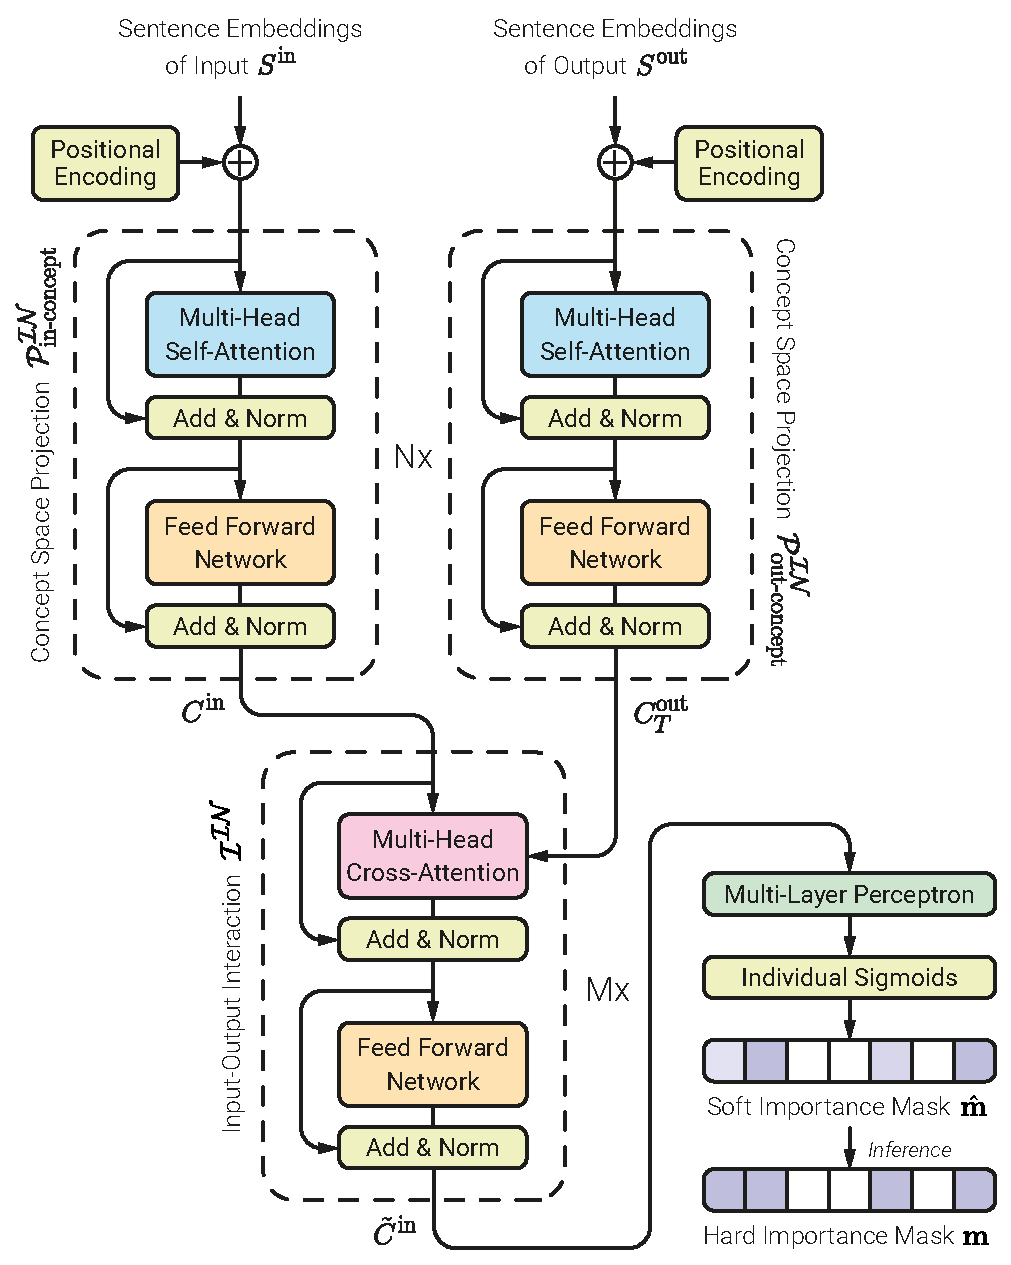
\includegraphics[width=0.6\textwidth]{figures/Fig-Interpreter-Architecture-V4.pdf}
    \caption{معماری شبکه‌ی مفسر ($\mathcal{IN}$)}\label{fig:chap4_architecture_interpreter}
\end{figure}

معماری این مفسر، ساختار سه‌مرحله‌ای مدل \lr{EBM} (بخش~\ref{sec:4-3-1}) را بازتاب می‌دهد و از یک ترنسفورمر دوسویه بهره می‌برد؛ اما تغییرات مشخصی در آن اعمال شده است تا از یک ارزیاب کلان به یک انتخاب‌گر پیش‌آیند با هدایت هدفمند تبدیل شود. جریان محاسبات در این معماری شامل مراحل زیر است:

\paragraph{۱. تصویرسازی فضای مفهومی.}
همانند مدل انرژی، پیش از هر پردازشی، یک لایه‌ی رمزگذاری موقعیتی به ماتریس‌های تعبیه‌ی ورودی و خروجی اضافه می‌شود تا اطلاعات ترتیبی حفظ گردد:
\begin{align}
    \tilde{S}^{\text{\lr{in}}} &= S^{\text{\lr{in}}} + E_{\text{\lr{pos}}}^{\text{\lr{in}}} \label{eq:chap4_interp_pos_enc_in} \\
    \tilde{S}^{\text{\lr{out}}} &= S^{\text{\lr{out}}} + E_{\text{\lr{pos}}}^{\text{\lr{out}}} \label{eq:chap4_interp_pos_enc_out}
\end{align}
سپس، این تعبیه‌ها از طریق ماژول‌های خودتوجهی به یک فضای مفهومی پویا تصویر می‌شوند. این دو ماژول تصویرساز مفسر ($\mathcal{P}_{\text{\lr{in-concept}}}^{\mathcal{IN}}$ و $\mathcal{P}_{\text{\lr{out-concept}}}^{\mathcal{IN}}$) از نظر معماری مشابه همتایان خود در \lr{EBM} طراحی شده‌اند (شامل $N$ لایه‌ی استاندارد ترنسفورمر). با این حال، پارامترهای ماژول‌ها در شبکه‌ی مفسر ($\alpha$) کاملاً از وزن‌های شبکه‌ی \lr{EBM} ($\theta$) مستقل بوده و منحصراً برای وظیفه‌ی استخراج ویژگی آموزش می‌بینند:
\begin{align}
    C^{\text{\lr{in}}} &= \mathcal{P}_{\text{\lr{in-concept}}}^{\mathcal{IN}}(\tilde{S}^{\text{\lr{in}}}) \label{eq:chap4_interp_concept_in} \\
    C^{\text{\lr{out}}} &= \mathcal{P}_{\text{\lr{out-concept}}}^{\mathcal{IN}}(\tilde{S}^{\text{\lr{out}}}) \label{eq:chap4_interp_concept_out}
\end{align}
از منظر طراحی معماری، هم‌سان‌سازی تعداد لایه‌های این ماژول‌ها با تصویرسازهای شبکه‌ی \lr{EBM} و استفاده از وزن‌های تصویرساز مدل انرژی برای مقداردهی اولیه‌ی تصویرساز مفسر، انتقال بازنمایی‌های مفهومی اولیه را تسهیل کرده و روند یادگیری مفسر را در استخراج ویژگی‌ها هموار می‌سازد.

\paragraph{۲. ماسک‌گذاری هدف و تعامل متمرکز.}
نقطه‌ی افتراق کلیدی مفسر با شبکه‌ی \lr{EBM}، در بلوک تعاملی آن‌ها نهفته است. در مدل انرژی، نیازمند ارزیابی انطباق‌پذیری کل پرامپت با کل پاسخ برای سنجش الگوهای کلان بودیم؛ اما در شبکه‌ی مفسر، تحلیل‌گر در پی شناسایی پیش‌آیندهای اثرگذار بر گزاره‌های معینی از خروجی ($T$) است. با این حال، مفسر نیازمند دریافت بافتار کامل پاسخ ($\mathbf{y}$) در بازنمایی‌های مفهومی خود است تا ساختار کلی متن حفظ شود.

بدین‌منظور، پیش از ورود به بلوک توجه متقاطع، شرطی‌سازی بر روی زیرمجموعه‌ی هدف از طریق اعمال بردار شاخص دودویی $\mathbf{m}_T \in {\{0, 1\}}^{N_{\text{\lr{max}}}}$ بر روی تانسور مفاهیم خروجی محقق می‌شود (که در آن به ازای $j \in T$ مقدار ۱ و در غیر این صورت ۰ قرار می‌گیرد):
\begin{equation}
    C^{\text{\lr{out}}}_T = \mathbf{m}_T \odot C^{\text{\lr{out}}} \label{eq:chap4_target_masking}
\end{equation}
سپس، تانسورهای $C^{\text{\lr{in}}}$ و $C^{\text{\lr{out}}}_T$ به ماژول تعاملی مفسر ($\mathcal{I}^{\mathcal{IN}}$) متشکل از $M$ لایه از بلوک‌های توجه متقاطع تغذیه می‌شوند. در این تقاطع، مفاهیم ورودی ($C^{\text{\lr{in}}}$) در نقش بردارهای پرسمان ($Q$)، و مفاهیم شرطی‌شده‌ی هدف ($C^{\text{\lr{out}}}_T$) در نقش بردارهای کلید ($K$) و ارزش ($V$) قرار می‌گیرند:
\begin{equation}\label{eq:chap4_interp_interaction}
    \tilde{C}^{\text{\lr{in}}} = \mathcal{I}^{\mathcal{IN}}\big(Q=C^{\text{\lr{in}}}, K=C^{\text{\lr{out}}}_T, V=C^{\text{\lr{out}}}_T\big)
\end{equation}
این ساختار به مفسر امکان می‌دهد تا ضمن بهره‌مندی از بافتار کامل پاسخ در لایه‌های پیشین، تمرکز توجه متقاطع را منحصراً معطوف به گزاره‌های هدف نموده و بازنمایی‌های پرامپت را بر پایه‌ی وابستگی به شاخص‌های $T$ به‌روزرسانی کند. در نتیجه، خروجی این بلوک ($\tilde{C}^{\text{\lr{in}}}$)، حاوی اطلاعات متمرکز بر تولید گزاره‌های هدف خواهد بود.

\paragraph{۳. استخراج امتیازات محلی.}
در گام بعدی، به‌جای فشرده‌سازی اطلاعات تمامی جملات به یک اسکالر واحد با استفاده از تجمیع مبتنی بر توجه، در مفسر نیازمند تولید یک خروجی مجزا به ازای تک‌تک جملات پرامپت هستیم تا درباره‌ی انتساب هر گزاره تصمیم‌گیری شود.

بدین‌منظور، خروجی بلوک توجه متقاطع ($\tilde{C}^{\text{\lr{in}}}$) مستقیماً به یک شبکه‌ی پرسپترون چندلایه‌ی کوچک (\lr{MLP}) با بعد خروجی ۱ تغذیه می‌شود. این لایه به‌صورت توزیع‌شده بر روی بازنمایی هر موقعیت (هر جمله‌ی ورودی) به‌طور مستقل عمل می‌کند. خروجی این لایه، برداری از امتیازات خام یا لوجیت‌ها است ($\mathbf{z} \in \mathbb{R}^{N_{\text{\lr{max}}}}$) که نشان‌دهنده‌ی اهمیت اولیه‌ی هر جمله‌ی پرامپت در ارتباط با خروجی هدف است:
\begin{equation}\label{eq:chap4_interp_logits}
    \mathbf{z} = \text{\lr{MLP}}(\tilde{C}^{\text{\lr{in}}})
\end{equation}

\paragraph{۴. آزادسازی پیوسته و تقریب توزیع مستقل.}
برای تبدیل این امتیازات به یک انتخاب گسسته (ماسک اهمیت دودویی $\mathbf{m}$)، نیازمند یک عملگر مشتق‌پذیر هستیم تا شبکه‌ی مفسر بتواند در طی فرایند پس‌انتشار آموزش ببیند. در روش‌های پایه‌ی انتخاب ویژگی نظیر \lr{L2X}~\cite{chen2018learning}، از عملگر گامبل-سافت‌مکس استفاده می‌شود. این عملگر با فرض وجود یک بودجه‌ی احتمالی ثابت (مجموع احتمالات برابر ۱)، ویژگی‌ها را مجبور به رقابت در یک توزیع دسته‌بندی می‌کند و زیرمجموعه‌ای با اندازه‌ی ازپیش‌تعیین‌شده را برمی‌گزیند.

با این وجود، تحلیل ساختاری نشان می‌دهد که اعمال سافت‌مکس در این بستر با چالش‌های نظری و هندسی روبه‌رو است. از منظر نظری، عملگر سافت‌مکس برای مدل‌سازی دسته‌های مانعه‌الجمع طراحی شده است؛ در حالی که در پردازش زبان طبیعی، مفاهیم غالباً در چندین گزاره توزیع شده و نیازمند ارزیابی غیررقابتی و چندگانه هستند~\cite{stahlberg2022jam}. علاوه بر این، محدودیت ساختاری تنگنای سافت‌مکس~\cite{yang2018breaking} نشان می‌دهد که این عملگر به دلیل محدودیت‌های رتبه‌ی ماتریس در فضای پنهان، ظرفیت بازنمایی توزیع‌های واژگانی چندوجهی را ندارد~\cite{chang2022softmax}.

فراتر از این محدودیت‌های نظری، در معماری حاضر، ترکیب این قید رقابتی با مکانیزم توجه متقاطع به افت مقیاس بردارها می‌انجامد. هنگامی که سافت‌مکس بودجه‌ی احتمالی را میان چندین جمله‌ی گزینش‌شده تقسیم می‌کند، مقیاس بردار تعبیه‌ی هر جمله تقلیل می‌یابد. این کاهش مقیاس، در ورود به لایه‌ی توجه متقاطع شبکه‌ی انرژی، تمرکز محاسبات را تضعیف کرده و سبب می‌شود \lr{EBM} (که با بردارهای استاندارد آموزش دیده است) مقادیر نامتعارفی تولید کند. در نتیجه، الگوریتم بهینه‌ساز برای اجتناب از این تغییر مقیاس، مفسر را به سوی تخصیص تمام وزن به یک جمله‌ی منفرد سوق می‌دهد. اثبات تحلیلی و جزئیات ریاضی این پدیده در پیوست~\ref{app:appendix_softmax_bottleneck} ارائه شده است.

برای غلبه بر این چالش، در متدولوژی \lr{ESCI} از مدل‌سازی رقابتی عبور کرده و فرایند انتخاب را به‌عنوان مجموعه‌ای از توزیع‌های برنولی\enfootnote{Bernoulli distribution} مستقل مدل‌سازی کرده‌ایم. بدین‌منظور، بردار لوجیت‌ها وارد یک تابع سیگموئید می‌شود تا امتیاز هر جمله به‌صورت مجزا به بازه‌ی $(0, 1)$ نگاشت گردد:
\begin{equation}\label{eq:chap4_interp_sigmoid}
    \hat{\mathbf{m}} = \text{\lr{Sigmoid}}(\mathbf{z})
\end{equation}
این بردار احتمالات پیوسته ($\hat{\mathbf{m}}$)، همان ماسک نرم است که در فاز آموزش، مستقیماً بر روی تعبیه‌های ورودی اعمال می‌شود و امکان جریان هموار گرادیان‌ها را بدون تخریب مقیاس هندسی بردارها فراهم می‌سازد.

در فاز استنتاج، برای تولید ماسک سخت ($\mathbf{m}$)، با در نظر گرفتن یک حد آستانه‌ی کوچک ($\epsilon$)، جملاتی که امتیازشان بالاتر از این آستانه باشد انتخاب شده و درایه‌های معادل آن‌ها برابر با ۱ قرار می‌گیرند:
\begin{equation}\label{eq:chap4_interp_hard_mask}
    \mathbf{m} = \mathbb{I}(\hat{\mathbf{m}} > \epsilon)
\end{equation}

طراحی این شبکه‌ی مفسر مستقل که به‌صورت قطعی و در زمان‌ثابت یک بردار ماسک تولید می‌کند، از نظر ساختاری الهام‌گرفته از چارچوب \lr{L2X}~\cite{chen2018learning} است. با این تفاوت که به دلیل ماهیت زایا و پیچیده‌ی مدل‌های زبانی، محاسبه‌ی مستقیم اطلاعات متقابل غیرعملی است و در چارچوب \lr{ESCI}، شبکه‌ی مفسر به‌جای بیشینه‌سازی اطلاعات متقابل آماری، آموزش می‌بیند تا شکاف انرژی را در چشم‌انداز \lr{EBM} بهینه‌سازی کند؛ فرایندی که توابع زیان آن در بخش بعد فرمول‌بندی می‌شوند.


\subsection{تابع هدف مفسر}\label{sec:4-4-2}

پس از استخراج ماسک نرم $\hat{\mathbf{m}} = \mathcal{IN}(\mathbf{x}, \mathbf{y}, T; \alpha) \in {(0, 1)}^N$ از شبکه‌ی مفسر، پرامپت اصلی کاربر مطابق با تعاریف~\ref{def:chap1_mask_space} و~\ref{prob:chap1_causal_attribution} در فضای بازنمایی‌ها به دو زیرمجموعه تفکیک می‌شود:
نخست، زیرمجموعه‌ی پیش‌آیندهای اثرگذار گزینش‌شده ($\mathbf{x}_S$):
\begin{equation}
    \mathbf{x}_S = \mathbf{x} \odot \hat{\mathbf{m}}
\end{equation}
و دوم، زیرمجموعه‌ی متمم یا دورریز ($\mathbf{x}_{\text{\lr{discard}}}$) که فاقد وابستگی معنادار به گزاره‌های هدف تلقی می‌گردد:
\begin{equation}
    \mathbf{x}_{\text{\lr{discard}}} = \mathbf{x} \odot (\mathbf{1} - \hat{\mathbf{m}}) = \mathbf{x} \setminus \mathbf{x}_S
\end{equation}

هدف آموزش مفسر، یافتن ماسکی است که جملات حفظ‌شده در $\mathbf{x}_S$ اطلاعات کافی برای بازتولید گزاره‌های هدف ($\mathbf{y}_T$) را دارا باشند. در این معماری، مدل جانشین انرژی ($\mathcal{E}_{\text{\lr{LM}}}(\cdot, \cdot; \theta)$) نقش یک ناظر و منتقد ثابت را ایفا می‌کند. بنابراین در بهینه‌سازی پارامترهای مفسر ($\alpha$)، فرایند آموزش با بهره‌گیری از دانش موجود در چشم‌انداز انرژی، شکاف انرژی زیر را بیشینه می‌سازد:
\begin{equation}\label{eq:chap4_interpreter_objective}
    \hat{\alpha} = \arg\max_\alpha \mathbb{E}_{(\mathbf{x}, \mathbf{y}, T)} \Big[ \mathcal{E}_{\text{\lr{LM}}}\big(\mathbf{x} \odot (\mathbf{1} - \hat{\mathbf{m}}), \mathbf{y}_T; \theta\big) - \mathcal{E}_{\text{\lr{LM}}}\big(\mathbf{x} \odot \hat{\mathbf{m}}, \mathbf{y}_T; \theta\big) \Big]
\end{equation}
که در آن $\mathbf{y}_T = {(y_j)}_{j \in T}$ توالی جملات هدف خروجی بر مبنای تعریف~\ref{def:chap1_target_subset} است. این تابع هدف، مفسر را در دو جهت مکمل هدایت می‌کند:
\begin{itemize}
    \item \textbf{کمینه‌سازی انرژی جفت منتخب:} با کمینه شدن عبارت $\mathcal{E}_{\text{\lr{LM}}}(\mathbf{x} \odot \hat{\mathbf{m}}, \mathbf{y}_T; \theta)$، انرژی انطباق‌پذیری میان جملات پیش‌آیند منتخب و گزاره‌های هدف در دیدگاه مدل انرژی کاهش می‌یابد. این فشار تضمین می‌کند که پیش‌آیندهای استخراج‌شده با خروجی همسو بوده و شرط کفایت~\cite{deyoung2020eraser} در مسئله‌ی~\ref{prob:chap1_causal_attribution} ارضا شود.
    \item \textbf{بیشینه‌سازی انرژی جفت دورریز:} هم‌زمان، بیشینه شدن عبارت $\mathcal{E}_{\text{\lr{LM}}}(\mathbf{x} \odot (\mathbf{1} - \hat{\mathbf{m}}), \mathbf{y}_T; \theta)$ شبکه را ملزم می‌سازد تا بخش باقی‌مانده و ماسک‌شده‌ی پرامپت فاقد همخوانی با هدف باشد. این فشار متقابل تضمین می‌کند که مفسر هیچ پیش‌آیند اثرگذاری را در بخش دورریز رها نکرده باشد و شرط جامعیت~\cite{deyoung2020eraser} تأمین گردد.
\end{itemize}

علاوه بر این هدف‌گذاری تقابلی، برای جلوگیری از انتخاب بیش از حد جملات و هدایت مفسر به سوی استخراج توضیحی خلوت و متمرکز، عبارت منظم‌سازی خلوتی مبتنی بر نرم $L_1$ بر مبنای اصل ضرورت و فشردگی در مسئله‌ی~\ref{prob:chap1_causal_attribution} افزوده می‌شود. تابع زیان نهایی برای به‌روزرسانی وزن‌های مفسر ($\alpha$) به فرم زیر تعریف می‌گردد:
\begin{equation}\label{eq:chap4_interpreter_loss_final}
    \mathcal{L}_{\mathcal{IN}}(\alpha) = \mathcal{E}_{\text{\lr{LM}}}\big(\mathbf{x} \odot \hat{\mathbf{m}}, \mathbf{y}_T; \theta\big) - \mathcal{E}_{\text{\lr{LM}}}\big(\mathbf{x} \odot (\mathbf{1} - \hat{\mathbf{m}}), \mathbf{y}_T; \theta\big) + \lambda_{\text{\lr{sparse}}} \|\hat{\mathbf{m}}\|_1
\end{equation}
که در آن $\lambda_{\text{\lr{sparse}}}$ ضریب جریمه‌ی خلوتی است و بهینه‌سازی با استفاده از الگوریتم‌های مبتنی بر گرادیان برای کمینه‌سازی این زیان انجام می‌پذیرد.

به‌کارگیری مدل \lr{EBM} به‌عنوان ناظر برای آموزش شبکه‌ی استخراج‌گر متن، در امتداد چارچوب \lr{ENGINE}~\cite{tu2020engine} قرار دارد که نشان داد تقطیر دانش از یک چشم‌انداز انرژی می‌تواند یادگیری شبکه‌های استنتاج را در وظایف زبانی هدایت کند. در معماری \lr{ESCI}، شبکه‌ی مفسر به‌جای تولید توالی جدید، با حفظ ساختار متنی، یک ماسک پیوسته بر روی ویژگی‌های موجود اعمال می‌کند. سیگنال گرادیانی پیوسته‌ای که از سمت مدل انرژی به مفسر پس‌انتشار می‌یابد، بدون نیاز به داده‌های نظارتی و برچسب‌دار انتساب، مفسر را به سوی شناسایی زیرمجموعه‌ای متمرکز و کافی از پیش‌آیندهای اثرگذار هدایت می‌نماید.



\section{آموزش مشترک و بهینه‌سازی تناوبی}\label{sec:4-5}

علی‌رغم کارایی مفسر ($\mathcal{IN}$) در استخراج ویژگی‌ها از طریق بیشینه‌سازی شکاف انرژی (معادله‌ی~\ref{eq:chap4_interpreter_objective})، اعمال ماسک بر روی جملات پرامپت ($\mathbf{x}_S = \mathbf{x} \odot \hat{\mathbf{m}}$) چالش ساختاری مشخصی به‌همراه دارد. اگرچه پردازش متن در سطح جمله از تخریب گرامری جلوگیری می‌کند، اما حذف بخش‌هایی از گزاره‌ها می‌تواند پیوستگی بافتاری ورودی را تغییر دهد و ریسک بروز شوک توزیعی~\cite{hsia2024goodhart} را به‌همراه داشته باشد. اگرچه مدل جانشین \lr{EBM} در فاز پیش‌آموزش (بخش~\ref{sec:4-3-2}) پرامپت‌های جزئی را مشاهده کرده است، اما ممکن است پاسخ‌های جدید مدل زبانی در برابر این پرامپت‌های تقلیل‌یافته‌ی خاص، رفتارهای متفاوتی را نسبت به توزیع اولیه‌ی آموزش نشان دهند که دقت ارزیابی مدل انرژی را تحت تأثیر قرار دهد.

ایده‌ی بهره‌گیری از آموزش مشترک برای مهار خطای تغییر توزیع در شبکه‌های استخراج‌گر، در چارچوب‌هایی نظیر \lr{SOInter}~\cite{seyyedsalehi2024sointer} مورد توجه قرار گرفته است. با این حال، در دامنه‌ی تولید متون آزاد توسط مدل‌های زبانی خودهمبسته، خروجی‌ها ماهیتی چندوجهی دارند. از این رو، ما یک استراتژی بهینه‌سازی تناوبی طراحی کرده‌ایم که از طریق ارسال دوره‌ای پرامپت‌های تقلیل‌یافته به مدل هدف و دریافت پاسخ‌های آن، شبکه‌ی انرژی را با مشاهدات جدید کالیبره می‌سازد. طرح کلی این رویکرد در شکل~\ref{fig:chap4_pipeline_joint_training} به تصویر کشیده شده است.

\begin{figure}[ht]
    \centering
    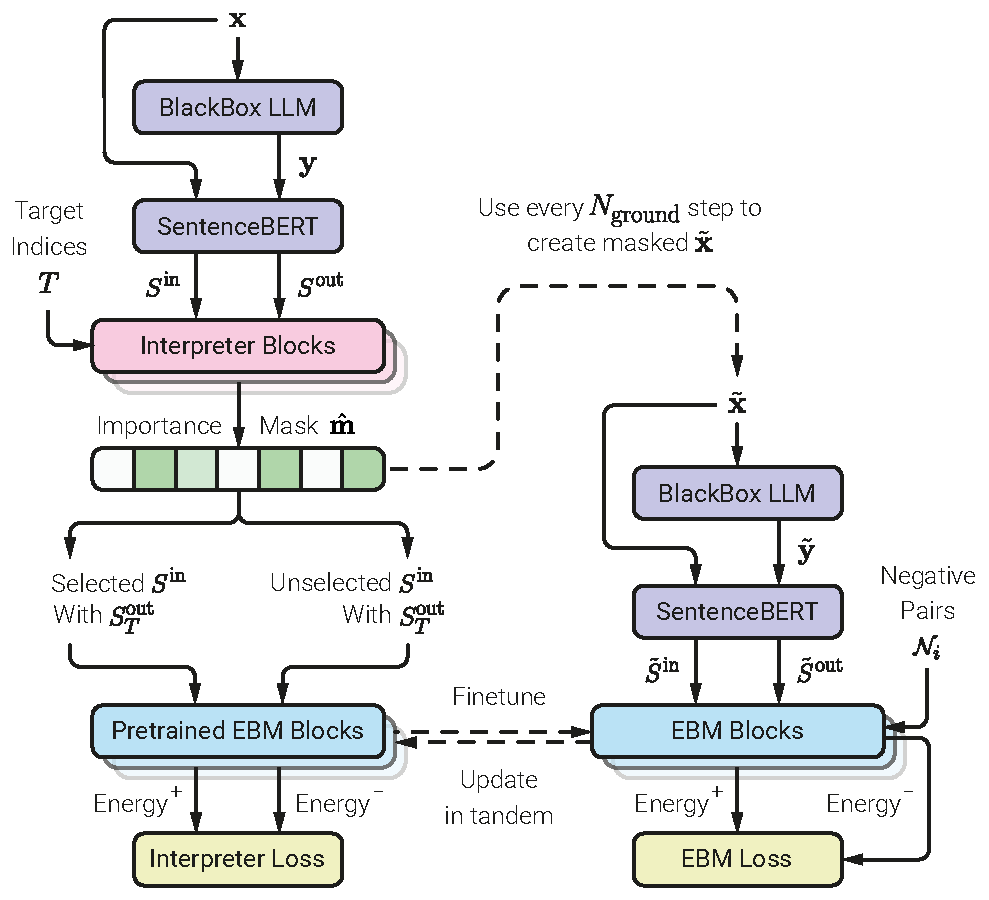
\includegraphics[width=0.76\textwidth]{figures/Fig-Joint-Training-Pipeline-V4.pdf}
    \caption{خط‌لوله‌ی آموزش مشترک شبکه‌های مفسر و انرژی}\label{fig:chap4_pipeline_joint_training}
\end{figure}

در این الگوریتم، پارامترهای مفسر ($\alpha$) و پارامترهای شبکه‌ی انرژی ($\theta$) به‌صورت متناوب و در دو گام مجزا به‌روزرسانی می‌شوند. فرض کنید در گام آموزشی $k$ام قرار داریم و مقادیر پارامترها به‌صورت $\theta^{(k)}$ و $\alpha^{(k)}$ نمادگذاری شده‌اند.

\paragraph{گام اول: به‌روزرسانی مفسر (تقطیر دانش).}
در گام‌های آموزشی متعارف (سمت چپ شکل~\ref{fig:chap4_pipeline_joint_training})، پارامترهای شبکه‌ی انرژی ($\theta^{(k-1)}$) ثابت نگه‌داشته می‌شوند. مفسر، بردار ماسک نرم $\hat{\mathbf{m}}$ را با استفاده از تقریب برنولی (معادله‌ی~\ref{eq:chap4_interp_sigmoid}) تولید می‌کند. سپس پارامترهای آن ($\alpha$) از طریق گرادیان نزولی به‌روزرسانی می‌شوند تا تابع هدف مفسر (معادله‌ی~\ref{eq:chap4_interpreter_loss_final}) را کمینه کنند:
\begin{equation}\label{eq:chap4_update_interpreter}\vspace{0.25cm}
    \begin{split}
        \alpha^{(k)} \leftarrow \alpha^{(k-1)} - \eta_{\alpha} \nabla_\alpha \Big( &\mathcal{E}_{\text{\lr{LM}}}\big(\mathbf{x} \odot \hat{\mathbf{m}}, \mathbf{y}_T; \theta^{(k-1)}\big) \\
        &- \mathcal{E}_{\text{\lr{LM}}}\big(\mathbf{x} \odot (\mathbf{1} - \hat{\mathbf{m}}), \mathbf{y}_T; \theta^{(k-1)}\big) + \lambda_{\text{\lr{sparse}}} \|\hat{\mathbf{m}}\|_1 \Big)
    \end{split}\vspace{0.25cm}
\end{equation}
که در آن $\eta_{\alpha}$ نرخ یادگیری مفسر و $\hat{\mathbf{m}} = \mathcal{IN}(\mathbf{x}, \mathbf{y}, T; \alpha^{(k-1)})$ است. در این گام، مفسر دانش موجود در چشم‌انداز انرژی را برای ارتقای قدرت استخراج پیش‌آیندها تقطیر می‌کند.

\paragraph{گام دوم: تطبیق و لنگراندازی دوره‌ای.}
به‌منظور هم‌تراز نگه‌داشتن \lr{EBM} با توزیع ماسک‌های تولیدشده توسط مفسر، هر $N_{\text{\lr{ground}}}$ گام یک‌بار، فرایند لنگراندازی دوره‌ای\enfootnote{periodic grounding} اجرا می‌شود (سمت راست شکل~\ref{fig:chap4_pipeline_joint_training}). ابتدا ماسک سخت بر پرامپت اعمال می‌شود تا جملات فیلترشده از ورودی حذف شوند (معادله‌ی~\ref{eq:chap4_interp_hard_mask}):
\begin{equation*}
    \mathbf{x}_{\text{\lr{hard}}} = \mathbf{x} \odot \mathbb{I}(\hat{\mathbf{m}} > \epsilon)
\end{equation*}
سپس، این پرامپت از طریق رابط برنامه‌نویسی به مدل جعبه‌سیاه ارسال می‌گردد تا خروجی متناظر آن ثبت شود:
\begin{equation}\label{eq:chap4_query_llm}
    \tilde{\mathbf{y}} = f_\theta(\mathbf{x}_{\text{\lr{hard}}})
\end{equation}
این فرایند یک جفت مشاهداتی جدید $(\mathbf{x}_{\text{\lr{hard}}}, \tilde{\mathbf{y}})$ فراهم می‌سازد که بازتاب‌دهنده‌ی رفتار مدل جعبه‌سیاه در قبال پرامپت تقلیل‌یافته است. در نهایت، پارامترهای شبکه‌ی انرژی ($\theta$) بر روی این داده‌ی جدید با استفاده از تابع زیان دوگانه (معادله‌ی~\ref{eq:chap4_ebm_total_loss}) تنظیم می‌شوند.

در این گام، به دلیل نبود پاسخ انسانی مرجع برای پرامپت مخدوش $\mathbf{x}_{\text{\lr{hard}}}$، مجموعه‌ی منفی وفاداری ($\mathcal{N}^{\text{\lr{fid}}}$) با نمونه‌برداری از سایر مدل‌های پایه بازتعریف می‌شود تا تضاد توزیعی در آموزش \lr{InfoNCE} برقرار بماند. با در نظر داشتن $\tilde{\mathcal{N}}$ به‌عنوان مجموعه‌ی منفی متناظر، رابطه‌ی به‌روزرسانی پارامترهای انرژی به‌صورت زیر خواهد بود:
\begin{equation}\label{eq:chap4_update_ebm}\vspace{0.05cm}
    \theta^{(k)} \leftarrow \theta^{(k-1)} - \eta_{\theta} \nabla_\theta \Big( (1-\lambda)\mathcal{L}_{\text{\lr{fidelity}}}(\mathbf{x}_{\text{\lr{hard}}}, \tilde{\mathbf{y}}, \tilde{\mathcal{N}}) + \lambda\mathcal{L}_{\text{\lr{dep}}}(\mathbf{x}_{\text{\lr{hard}}}, \tilde{\mathbf{y}}) \Big)
\end{equation}

\begin{algorithm}[ht]
\caption{آموزش مشترک شبکه‌های مفسر و انرژی (بهینه‌سازی تناوبی)}\label{alg:chap4_joint_opt}
\begin{algorithmic}[1]
\vspace{0.25cm}
\Require{} پرامپت $\mathbf{x}$، خروجی $\mathbf{y}$، شاخص‌های هدف خروجی $T$، مفسر مقداردهی‌شده $\mathcal{IN}_\alpha$، مدل جانشین پیش‌آموزش‌دیده $\mathcal{E}_\theta$، بازه‌ی لنگراندازی $N_{\text{\lr{ground}}}$، حد آستانه‌ی $\epsilon$
\vspace{0.25cm}
\For{هر گام آموزشی $k$}
    \vspace{0.15cm}
    \State{} \textbf{// گام اول: به‌روزرسانی مفسر}
    \vspace{0.15cm}
    \State{} تولید ماسک نرم پیوسته: $\hat{\mathbf{m}} \leftarrow \text{\lr{Sigmoid}}(\mathcal{IN}(\mathbf{x}, \mathbf{y}, T; \alpha^{(k-1)}))$
    \State{} تفکیک زیرمجموعه‌ها: $\mathbf{x}_S = \mathbf{x} \odot \hat{\mathbf{m}}$ و $\mathbf{x}_{\text{\lr{discard}}} = \mathbf{x} \odot (\mathbf{1} - \hat{\mathbf{m}})$
    \State{} \parbox[t]{0.95\linewidth}{محاسبه‌ی گرادیان و به‌روزرسانی $\alpha^{(k)}$ جهت کمینه‌سازی زیان مفسر (معادله‌ی~\ref{eq:chap4_update_interpreter}) با منتقد ثابت $\mathcal{E}_{\theta^{(k-1)}}$}
    \vspace{0.25cm}
    \State{} \textbf{// گام دوم: لنگراندازی دوره‌ای و تنظیم ظریف \lr{EBM}}
    \vspace{0.15cm}
    \If{$k \pmod{N_{\text{\lr{ground}}}} == 0$}
        \State{} اعمال ماسک سخت: $\mathbf{x}_{\text{\lr{hard}}} \leftarrow \mathbf{x} \odot \mathbb{I}(\hat{\mathbf{m}} > \epsilon)$
        \State{} استعلام از مدل جعبه‌سیاه: $\tilde{\mathbf{y}} \leftarrow f_\theta(\mathbf{x}_{\text{\lr{hard}}})$
        \State{} \parbox[t]{0.9\linewidth}{محاسبه‌ی گرادیان و به‌روزرسانی $\theta^{(k)}$ جهت کمینه‌سازی تابع زیان انرژی (معادله‌ی~\ref{eq:chap4_update_ebm}) برای جفت $(\mathbf{x}_{\text{\lr{hard}}}, \tilde{\mathbf{y}})$}
    \vspace{0.15cm}
    \Else{}
        \State{} انجماد مدل انرژی: $\theta^{(k)} \leftarrow \theta^{(k-1)}$
    \EndIf{}
    \vspace{0.25cm}
\EndFor{}
\end{algorithmic}
\end{algorithm}

این فرایند لنگراندازی (الگوریتم~\ref{alg:chap4_joint_opt})، دارای دو توجیه نظری در ادبیات یادگیری ماشین است که اجرای آن را برای تثبیت مدل تقویت می‌کند. نخست، بر اساس واکاوی تو و همکاران (۲۰۲۰)~\cite{tu2020improving} پیرامون آموزش مشترک شبکه‌های انرژی و استنتاج، در صورت عدم‌انطباق پویای دو شبکه، مدل انرژی ممکن است دچار نواحی کم‌انرژی کاذب گردد؛ چرا که مفسر در فرایند بهینه‌سازی ممکن است ماسک‌هایی را برگزیند که در چشم‌انداز اولیه‌ی مدل منجمد به‌اشتباه دارای انرژی پایینی هستند. استعلام دوره‌ای از مدل هدف، چشم‌انداز انرژی را با مشاهدات متنی واقعی کالیبره کرده و این عدم‌تعادل‌ها را تعدیل می‌سازد.

افزون بر این، ساوینوف و همکاران (۲۰۲۲)~\cite{savinov2022stepunrolled} در معماری \lr{SUNDAE} نشان دادند مدل‌هایی که با ورودی‌های مخدوش سروکار دارند، چنانچه صرفاً بر روی یک توزیع نویز ایستا آموزش ببینند، در مواجهه با توزیع‌های متغیر نویز با افت تعمیم‌پذیری روبه‌رو می‌شوند. در چارچوب \lr{ESCI}، با تکامل پارامترهای مفسر، توزیع ماسک‌های اعمال‌شده نیز تغییر می‌کند. از این رو، لنگراندازی دوره‌ای از نظر ساختاری با مکانیزم باز کردن گام‌به‌گام\enfootnote{step-unrolling} همسویی دارد؛ فرایندی که تضمین می‌نماید مدل انرژی با توزیع پویای ماسک‌های ایجادشده توسط مفسر همگام باقی بماند.

بدین‌ترتیب، چارچوب دوفازی \lr{ESCI} با تلفیق مدل‌سازی انرژی در سطح گزاره و استنتاج مستهلک‌شده در شبکه‌ی مفسر، رویکردی ساختاریافته برای انتساب در سطح جمله در مدل‌های زبانی جعبه‌سیاه فراهم می‌آورد. این متدولوژی با جایگزینی استعلام‌های مکرر و پرهزینه در زمان استنتاج با یک ارزیابی پیش‌رو، و بهره‌گیری از بهینه‌سازی تناوبی و لنگراندازی دوره‌ای جهت تثبیت بازنمایی‌ها در برابر شوک توزیعی، امکان ممیزی عینی مدل‌های تجاری را بدون نیاز به‌دسترسی به وزن‌ها یا گرادیان‌های درونی فراهم می‌سازد. ارزیابی جامع تجربی، سنجش وفاداری و تحلیل کمّی عملکرد این چارچوب در مقایسه با روش‌های خط‌پایه در فصل~\ref{chap:chapter5_experiments} ارائه خواهد شد.

% !TEX root = ../thesis.tex
% ==============================================================================
%  CHAPTER 5: EXPERIMENTS & RESULTS (فصل پنجم: آزمایش‌ها و نتایج تجربی) (chapters/chapter5_experiments.tex)
% ==============================================================================
%  This chapter presents empirical validation, benchmark evaluations,
%  interventional ablation studies, efficiency metrics, and more.
% ==============================================================================

\chapter{آزمایش‌ها و ارزیابی نتایج}\label{chap:chapter5_experiments}

این فصل به تحلیل جامع و نظام‌مند تجربی چارچوب مفسر جانشین مبتنی بر انرژی (\lr{ESCI}) اختصاص دارد. آزمایش‌ها به‌گونه‌ای طراحی شده‌اند که عملکرد این روش را در رویارویی با معماری‌های متنوع زبانی، در دو محیط استنتاجی متفاوت و در مقایسه با طیفی از روش‌های جعبه‌سیاه، جعبه‌خاکستری و جعبه‌سفید مورد ارزیابی قرار دهند. در این راستا، ابتدا مدل‌های هدف، مجموعه‌داده‌ها و خطوط پایه‌ی مقایسه‌ای معرفی می‌شوند؛ سپس ویژگی‌های هندسی چشم‌انداز انرژی و پویایی آموزش مفسر کالبدشکافی شده و در نهایت، میزان معقولیت و وفاداری تجربی مفسر در ارزیابی وابستگی‌های گزاره‌ای و کارایی محاسباتی آن سنجیده می‌شود.


\section{مدل‌ها، مجموعه‌داده‌ها و تنظیمات اجرایی}\label{sec:5-1}

برای تضمین جامعیت و تکرارپذیری آزمایش‌ها، انتخاب مدل‌های هدف، دادگان و خطوط پایه با در نظر گرفتن تنوع ساختاری و محدودیت‌های عملیاتی دنیای واقعی صورت گرفته است. در این بخش، جزئیات هر یک از این مؤلفه‌ها تشریح می‌گردد.


\subsection{مدل‌های هدف}\label{sec:5-1-1}

انتخاب مدل‌های زبانی هدف در این پژوهش با رویکردی راهبردی انجام شده است تا پوشش مناسبی بر روی تنوع معماری‌های مدرن و سطوح مختلف دسترسی فراهم آید. با توجه به صورت‌مسئله‌ی اصلی این پایان‌نامه مبنی بر ارزیابی مستقل از مدل و ممیزی سیستم‌های مسدود، ما در تمامی آزمایش‌ها با هر سه مدل با فرض عدم‌دسترسی به معماری و وزن‌های داخلی مدل پیش می‌رویم. با این حال، به‌دلیل محدودیت‌های منابع محاسباتی و هزینه‌های بالای فراخوانی \lr{API}ها، بخش عمده‌ی آزمایش‌های اعتبارسنجی بر روی دو مدل متن‌باز انجام گرفته است و مدل تجاری تنها در بخش‌های منتخبی برای سنجش کارایی چارچوب در سناریوی مسدود مورد استفاده قرار می‌گیرد. شایان ذکر است که تمامی مدل‌های انتخاب‌شده، نسخه‌های هم‌ترازشده و مبتنی بر دستورالعمل هستند تا ارزیابی‌ها در یک بستر تعاملی واقعی انجام گیرد؛ با این وجود، ارزیابی مفسر بر روی این سه مدل با معماری‌های زیربنایی کاملاً متفاوت، نشان می‌دهد که چارچوب پیشنهادی به جزئیات پیاده‌سازی یا گراف محاسباتی یک خانواده‌ی خاص از مدل‌ها وابسته نیست.

\paragraph{مدل \lr{Llama–3.1–8B–Instruct}:} این مدل که توسط شرکت متا توسعه یافته است~\cite{grattafiori2024llama3}، در حال حاضر به‌عنوان یکی از خطوط پایه‌ی استاندارد مدل‌های متراکم و متن‌باز در ابعاد کوچک تا متوسط شناخته می‌شود. همان‌طور که از پسوند \lr{–Instruct} پیداست، نسخه‌ی حاضر تحت فرایند تنظیم مبتنی بر دستورالعمل قرار گرفته است؛ رویکردی که تمرکز شبکه را از تکمیل ساده‌ی متن، به سوی درک و پاسخ‌گویی دقیق به دستورات کاربر تغییر می‌دهد. از منظر معماری، این مدل بر پایه‌ی مکانیسم توجه پرسمان گروهی\enfootnote{grouped-query attention} (\lr{GQA})~\cite{ainslie2023gqa} استوار است. در این مکانیسم، برخلاف توجه چندسره‌ی استاندارد که هر پرسمان، کلید و ارزش اختصاصی خود را دارد، پرسمان‌ها دسته‌بندی شده و هر گروه از یک جفت کلید و ارزش مشترک استفاده می‌کنند. این امر اگرچه کارایی محاسباتی و سرعت استنتاج را به‌طور چشمگیری ارتقا می‌دهد، اما مسیرهای توزیع اطلاعات و جریان وابستگی‌های لایه‌ای را نسبت به ترنسفورمرهای اولیه دگرگون می‌سازد.

\paragraph{مدل \lr{Gemma–2–9B–It}:} پسوند \lr{–It} در این مدل متن‌باز از شرکت گوگل~\cite{gemmateam2024gemma2} نیز نشان‌دهنده‌ی تنظیم آن مبتنی بر دستورالعمل‌هاست. این مدل که بر پایه‌ی پژوهش‌های بنیادین به‌کاررفته در توسعه‌ی مدل‌های خانواده‌ی \lr{Gemini}~\cite{comanici2025gemini25} ساخته شده است، دارای ساختار متفاوتی نسبت به خانواده‌ی \lr{Llama} است. مدل \lr{Gemma-2} از مکانیسم‌های نوین توجه متناوب محلی و سراسری\enfootnote{alternating local-global attention} بهره می‌برد؛ به این معنا که لایه‌های شبکه به‌صورت یک‌درمیان، به‌جای پردازش کل توالی (سراسری)، تنها به یک پنجره‌ی لغزان از کلمات مجاور (محلی) توجه می‌کنند. این ساختار پله‌ای، شعاع درک بافتار را به بخش‌های مجزا تقسیم کرده و ردیابی وابستگی‌های طولانی‌مدت را تغییر می‌دهد. افزون بر این، جایگزینی توابع فعال‌ساز استاندارد با \lr{GeGLU}~\cite{shazeer2020glu} (که با افزودن یک دروازه‌ی ضربی، تبدیلات غیرخطی پیچیده‌تری در لایه‌های پیش‌خور ایجاد می‌کند) و استفاده از تکنیک کنترل نرم لوجیت‌ها\enfootnote{logit soft-capping} برای محدود کردن رشد مقادیر فعال‌سازی پیش از لایه‌ی سافت‌مکس، توزیع احتمالات خروجی را تحت تأثیر قرار می‌دهد.

\paragraph{مدل \lr{GPT–4o–Mini}:} این مدل نماینده‌ی سیستم‌های تجاری، اختصاصی و مسدود در اکوسیستم فعلی هوش مصنوعی است~\cite{openai2023gpt4}. در مرحله‌ی هم‌ترازی با دستورالعمل‌های کاربر، خروجی‌های این مدل تحت تأثیر یادگیری تقویتی با بازخورد انسانی\enfootnote{RL from human feedback} (\lr{RLHF})~\cite{ouyang2022training} قرار گرفته‌اند. این فرایند، پیش‌فرض‌های رفتاری خاصی (مانند تکیه‌کلام‌های محاوره‌ای، لحن مؤدبانه و الگوهای امتناع از پاسخ) را به مدل اضافه می‌کند که غالباً در مسیر انتساب گزاره‌ای به‌صورت نویز ظاهر می‌شوند. افزون بر این، بر مبنای تحلیل‌ها و گزارش‌های فنی در جامعه‌ی پژوهشی، این گمانه‌زنی مطرح است که زیرساخت محاسباتی این سیستم‌ها از معماری ترکیب خلوت خبرگان\enfootnote{sparse mixture of experts} (\lr{MoE})~\cite{fedus2022switch} بهره می‌برد. در این معماری، به‌جای فعال‌سازی تمامی پارامترها برای هر توکن، یک شبکه‌ی مسیریاب در هر لایه تنها زیرمجموعه‌ای از متخصص‌ها را فعال می‌کند. این طراحی منجر به شکل‌گیری یک مسیر محاسباتی پویا و ناپیوسته می‌گردد که تقریب رفتار خارجی آن را در سطح جمله، به سناریویی چالش‌برانگیز برای مفسرهای مستقل از مدل تبدیل می‌نماید.


\subsection{مجموعه‌داده‌ها}\label{sec:5-1-2}

ارزیابی روش‌های تفسیرپذیری در وظایف تولید متن آزاد با چالش اساسی فقدان مجموعه‌داده‌های استاندارد با حقیقت پایه‌ی قطعی برای انتساب در سطح جمله روبه‌روست. ریشه‌ی این موضوع در تفاوت ماهویِ وظیفه‌ی تفسیر تولید آزاد با وظایف دسته‌بندی بسته نهفته است. در تولید یک پاراگراف آزاد توسط مدل‌های زبانی بزرگ، فرایند انتساب باید مشخص سازد که مدل در تولید هر گزاره، بر کدام جملات پرامپت تکیه کرده است. از آنجا که فرایند پردازش در سامانه‌های مسدود در قالب یک جعبه‌سیاه پنهان است، حقیقت پایه‌ی طلایی جهان‌شمولی برای آن وجود ندارد؛ لذا ارزیابی مفسر در این شرایط، متکی بر بررسی تغییرات رفتاری مدل از طریق اعمال مداخلات کنترل‌شده در ورودی خواهد بود.

با این وجود، در ادبیات پژوهش، گاهاً برای ایجاد یک معیار ارزیابی اولیه، تلاش می‌شود تا عملکرد مفسرها با انتساب و قضاوت انسانی مقایسه گردد؛ بدین‌معنا که بررسی شود آیا جملات انتخاب‌شده توسط مفسر، با جملاتی که ناظر انسانی آن‌ها را برای تولید پاسخ ضروری می‌داند، هم‌خوانی دارند یا خیر. اما حتی در چنین ارزیابی‌هایی، استفاده از مجموعه‌داده‌های موجود برای ارزیابی متدولوژی حاضر (که در سطح جمله و برای تولید متن آزاد طراحی شده است) با محدودیت‌هایی مواجه است. چالش اصلی آن است که در مجموعه‌داده‌های دارای برچسب انتساب، یک پاسخ نمونه‌ی ثابت به بخش خاصی از ورودی نسبت داده شده است. هنگامی که مدل زبانی با دریافت همان پرامپت، یک پاسخ جدید و پویا تولید می‌کند (که غالباً با متن مرجع مجموعه‌داده متفاوت است)، برچسب‌های انتساب ازپیش‌تعیین‌شده، اعتبار مستقیم خود را برای ارزیابی انتساب در قبال این پاسخ جدید از دست می‌دهند.

بررسی مجموعه‌داده‌های پرکاربرد در پردازش زبان طبیعی، این محدودیت‌ها را نشان می‌دهد. برای نمونه، مجموعه‌داده‌ی \href{https://huggingface.co/datasets/stanfordnlp/coqa/}{\lr{CoQA}}~\cite{reddy2019coqa} با وجود کاربرد گسترده، خروجی‌هایی در حد یک کلمه یا یک جمله‌ی بسیار کوتاه دارد و فاقد ساختار لازم برای ارزیابی متون چندجمله‌ای است. مجموعه‌داده‌ی \href{https://huggingface.co/datasets/hotpotqa/hotpot_qa}{\lr{HotpotQA}}~\cite{yang2018hotpotqa} اگرچه دارای حقایق پشتیبان مشخصی در متن است، اما پاسخ‌های آن صرفاً محدود به یک یا دو کلمه‌اند که با صورت‌مسئله‌ی ما (ارزیابی تولید متون طولانی) هم‌خوانی ندارد. از سوی دیگر، مجموعه‌داده‌ی \href{https://huggingface.co/datasets/StonyBrookNLP/tellmewhy}{\lr{TellMeWhy}}~\cite{lal2021tellmewhy} شامل حاشیه‌نویسی‌های انسانی برای پشتیبانی از استدلال‌هاست، اما علاوه بر کوتاه بودن خروجی‌ها، با چالش تفاوت پاسخ‌های تولیدی روبه‌روست. در نهایت، مجموعه‌داده‌های تولید متن بدون قید نظیر \href{https://huggingface.co/datasets/Salesforce/wikitext}{\lr{WikiText}}~\cite{merity2017pointer} نیز اگرچه برای تولید آزاد کاربرد دارند، اما به‌دلیل ماهیت ادامه‌نویسی (که در آن مدل غالباً به دانش پارامتریک و درونی خود برای ادامه‌ی متن تکیه می‌کند)، پیوند دادن خروجی به جملات محدود پرامپت را دشوار و فاقد لنگرگاه موضوعی مشخص می‌سازند.

برای رفع این محدودیت‌ها، ما به بسترهایی نیاز داریم که در آن‌ها، علی‌رغم آزاد بودن متن تولیدی، یک لنگرگاه معنایی میان پرامپت و پاسخ وجود داشته باشد تا بتوان رفتار مدل را ردیابی کرد. بر این اساس، آزمایش‌های ما بر روی دو مجموعه‌داده‌ی منتخب انجام می‌پذیرد که هر یک جنبه‌ای متفاوت از توانمندی مفسر را به چالش می‌کشند.

\subsubsection{مجموعه‌داده‌ی \lr{HC3}}\label{sec:5-1-2-1}

برای ارزیابی مفسر در محیط مکالمات روزمره، پرسش و پاسخ آزاد و تولید متن بدون محدودیت ساختاری، از پیکره‌ی مقایسه‌ای انسان و چت‌جی‌پی‌تی\enfootnote{Human ChatGPT Comparison Corpus} که به اختصار \href{https://huggingface.co/datasets/Hello-SimpleAI/HC3/}{\lr{HC3}}~\cite{guo2023closechatgpthumanexperts} نامیده می‌شود، بهره بردیم. این مجموعه‌داده‌ی چنددامنه‌ای شامل ده‌ها هزار پرسش استخراج‌شده از منابع متنوعی نظیر حوزه‌های مالی، پزشکی، حقوقی و پرسش‌های عمومی از انجمن‌های \lr{Reddit} (مانند \lr{ExplainLikeImFive} یا \lr{ELI5}) می‌باشد. 

دلیل اصلی انتخاب \lr{HC3} این است که برخلاف وظایف ادامه‌نویسی محض (نظیر \lr{WikiText})، ساختار پرسش و پاسخ در آن یک لنگرگاه موضوعی و گزاره‌ای شفاف ایجاد می‌کند. در این ساختار، هرچند مدل برای تولید یک پاراگراف طولانی آزاد است، اما پاسخ تولیدشده مستقیماً ملزم به پاسخ‌گویی به مفاهیم مطرح‌شده در پرسش کاربر است. در نتیجه، اگرچه برچسب انتساب قطعی انسانی در مجموعه‌داده وجود ندارد، اما الزام مدل به پاسخ‌گویی به صورت‌مسئله، مبنایی معقول فراهم می‌سازد تا بتوان گزاره‌های خروجی را به بخش‌های متناظر در پرامپت ارجاع داد.

در خط‌لوله‌ی اجرایی ما، ستون پرسش (\lr{Question}) از مجموعه‌داده به‌عنوان پرامپت ورودی در نظر گرفته می‌شود و سپس به مدل هدف (به‌عنوان مثال \lr{GPT-4o-Mini}) داده می‌شود تا پاسخ آزاد خود را تولید کند. همچنین، از پاسخ انسانی (\lr{Human Answer}) که در مجموعه‌داده موجود است، به‌عنوان نمونه‌ی منفی در آموزش تقابلی شبکه‌ی انرژی استفاده می‌شود. جدول~\ref{tab:chap5_hc3_sample} یک نمونه‌ی واقعی از پرسش، پاسخ مدل و پاسخ انسانی را در این مجموعه‌داده نشان می‌دهد.

\begin{table}[!ht]
    \centering
    \footnotesize
    \caption{نمونه‌ای از داده‌های استخراج‌شده از مجموعه‌داده‌ی \lr{HC3}}\label{tab:chap5_hc3_sample}
    \linespread{1.15}\selectfont
    \renewcommand{\arraystretch}{1.5}
    \setlength{\aboverulesep}{0pt}
    \setlength{\belowrulesep}{0pt}
    
    \begin{tabularx}{\textwidth}{@{} 
        >{\columncolor{white}[\tabcolsep][0pt]\hsize=0.4\hsize}X 
        >{\columncolor{white}[2.65pt][\tabcolsep]\setLTR\hsize=1.6\hsize}X 
        @{}}
        \toprule

        \rowcolor{gray!15} \centering\arraybackslash\raisebox{0.05cm}[0pt][0pt]{\textbf{بخش}} & \centering\arraybackslash\raisebox{0.05cm}[0pt][0pt]{\textbf{\rl{متن (ترجمه‌نشده به‌دلیل پردازش بومی مدل)}}} \vspace{0.05cm} \\
        \midrule
        \centering\textbf{\lr{Question}} & 
        \vspace{0.1cm} \lr{Why we experience the sensation of falling in our dreams / when we wake up. Title basically says it all. What causes this sensation? Why is it so seemingly universal and why is it so vivid relative to other physical sensations we experience in our dreams? Please explain like I'm five.} \vspace{0.1cm} \\ 
        \midrule
        \centering\textbf{\lr{GPT-4o-Mini Answer}} & 
        \vspace{0.1cm} \lr{Okay! Imagine your brain is like a big movie theater that shows dreams while you sleep. Sometimes, when you're dreaming, your body might feel like it's falling. This can happen because when you're asleep, your brain is still working hard, and it can get mixed up about what's real and what's not.} \par\vspace{-0.1cm}
        \lr{When you dream about falling, it's like your brain is playing a trick on you! It might be because your body is relaxing and your muscles are letting go, and your brain thinks, ``Whoa, I'm falling!'' This feeling can be really strong and surprising, just like a roller coaster ride!} \par\vspace{-0.1cm} % chktex 38
        \lr{A lot of people feel this way in their dreams because everyone's brain works in similar ways when they sleep. It's like a common movie that lots of people watch in their sleep!} \vspace{0.1cm} \\
        \midrule
        \centering\textbf{\lr{Human Answer}} & 
        \vspace{0.1cm} \lr{When you're in between deep sleep and the lighter sleep where it's easy to wake up, the sleep paralysis that stops you from acting out your dreams can do strange shit. Sometimes you'll be surfacing to wakefulness again when your brain accidently throws the sleep paralysis switch again. The sudden tension in the body can feel like falling to a sleep-frazzled mind, and it galvanizes you strongly it can even create the sensation you'd dropped onto the bed and bounced. You didn't. Your body just got switched into safe mode by accident.} \vspace{0.1cm} \\
        \bottomrule
    \end{tabularx}
\end{table}

\subsubsection{مجموعه‌داده‌ی \lr{WikiBio}}\label{sec:5-1-2-2}

در حالی که مجموعه‌داده‌ی \lr{HC3} بستر مناسبی برای ارزیابی در شرایط تولید متن آزاد فراهم می‌آورد، فقدان انتساب قطعی در مکالمات روزمره، ارزیابی کمی معقولیت انتساب را با دشواری روبه‌رو می‌کند. برای ایجاد یک لنگرگاه مشخص به‌عنوان شبه‌حقیقت پایه، ما از پارادایم تولید متن از روی داده‌های ساختاریافته\enfootnote{data-to-text generation} بهره گرفتیم. بدین‌منظور، از مجموعه‌داده‌ی \href{https://huggingface.co/datasets/michaelauli/wiki_bio}{\lr{WikiBio}}~\cite{lebret2016neural} استفاده شده است. این مجموعه‌داده شامل جداول اطلاعاتی ویکی‌پدیا (جعبه‌های اطلاعات) و پاراگراف‌های بیوگرافی متناظر با آن‌هاست. نقطه‌ی قوت \lr{WikiBio} در این است که اگرچه خروجی آن یک پاراگراف متنی پیوسته و آزاد است، اما محتوای این خروجی به حقایق مستقل موجود در یک جدول مشخص مقید شده است؛ به بیانی دیگر، این مجموعه‌داده استدلال مقید مبتنی بر داده را نشان می‌دهد. لذا ما با بهره‌گیری از این ویژگی، خط‌لوله‌ای طراحی کردیم تا این مجموعه‌داده را برای وظیفه‌ی انتساب در سطح جمله تطبیق دهیم. 

در گام نخست، ساختار جدولی ورودی (شامل کلید و مقدار) شکسته شده و هر حقیقت ایزوله به یک جمله‌ی مستقل زبان طبیعی (مانند «تاریخ تولد ۲۸ مارس ۱۹۶۹ است.») تبدیل می‌گردد. سپس، این جملات مستقل در قالب یک پرامپت صریح و با دستور عدم‌استفاده از دانش خارجی یا اضافات محاوره‌ای به مدل زبانی تغذیه می‌شوند تا مدل تلاش کرده و تا حد امکان، بیوگرافی نهایی را منحصراً از روی این پیش‌نیازهای اطلاعاتی تولید کند.

مزیت این پیکربندی در فاز ارزیابی نمایان می‌شود. از آنجا که هر جمله‌ی پرامپت، حامل یک یا چند حقیقت مشخص (مانند تاریخ، نام، یا آمار) است، ما می‌توانیم با ردیابی این موجودیت‌ها در متن تولیدشده توسط مدل، یک شبه‌حقیقت پایه‌ی ساختاریافته استخراج کنیم و مشخص سازیم که مدل برای نگارش هر جمله‌ی بیوگرافی، احتمالاً به کدام جملات پرامپت اتکا داشته است.

برای استخراج این نگاشت بدون نیاز به حاشیه‌نویسی پرهزینه‌ی انسانی، برنامه‌ی تطبیق معنایی و لغوی توسعه داده شد. در این الگوریتم، ابتدا جملات پرامپت (مبدأ) و پاسخ تولیدشده (مقصد) با استفاده از کتابخانه‌ی پردازش زبان \lr{spaCy}~\cite{honnibal2017spacy} توکن‌سازی و ریشه‌یابی می‌شوند. پس از حذف ایست‌واژه‌ها و علائم نگارشی، توکن‌های محتوایی کلیدی (شامل اسامی خاص، اعداد، صفت‌ها و افعال) استخراج می‌گردند. سپس، الگوریتم برای نگاشت هر جمله‌ی خروجی به پیش‌آیندهای اطلاعاتی متناظر در پرامپت، از یک رویکرد دومرحله‌ای استفاده می‌کند: ابتدا از اشتراک قطعی توکن‌ها بهره می‌برد و در صورت عدم‌تطابق (به‌دلیل تغییرات ساختار صرفی یا تغییرات جزئی واژگان)، از مکانیزم تطبیق فازی\enfootnote{fuzzy string matching} (با آستانه‌ی شباهت حداقل $0.75$) استفاده می‌کند. این خط‌لوله‌ی مکاشفه‌ای، مبنای ساخت خط‌پایه‌ی تطبیق رشته‌ای (\lr{StringMatching}) را تشکیل می‌دهد که به‌عنوان یک شبه‌حقیقت‌پایه برای اعتبارسنجی اولیه به‌کار می‌رود. این روند ثبت نگاشت میان گزاره‌های ورودی و گزاره‌های خروجی را تسهیل کرده و امکان سنجش عملکرد مفسر از بُعد معقولیت انتساب را در یک محیط عینی فراهم می‌سازد.

جدول~\ref{tab:chap5_wikibio_sample} نمونه‌ای از تبدیل داده‌های خام \lr{WikiBio} به فرمت پرامپت مورد استفاده در آزمایش‌ها، به‌همراه بیوگرافی تولیدشده توسط مدل \lr{Llama–3.1–8B–Instruct} و پاسخ انسانی مرجع را نشان می‌دهد.

\begin{table}[!ht]
    \centering
    \footnotesize
    \caption{نمونه‌ای از داده‌های استخراج‌شده از مجموعه‌داده‌ی \lr{WikiBio}}\label{tab:chap5_wikibio_sample}
    \linespread{1.15}\selectfont
    \renewcommand{\arraystretch}{1.5}
    \setlength{\aboverulesep}{0pt}
    \setlength{\belowrulesep}{0pt}

    \begin{tabularx}{\textwidth}{@{} 
        >{\columncolor{white}[\tabcolsep][0pt]\hsize=0.3\hsize}X 
        >{\columncolor{white}[2.65pt][\tabcolsep]\setLTR\hsize=1.7\hsize}X 
        @{}}
        \toprule

        \rowcolor{gray!15} \centering\arraybackslash\raisebox{0.05cm}[0pt][0pt]{\textbf{بخش}} & \centering\arraybackslash\raisebox{0.05cm}[0pt][0pt]{\textbf{\rl{متن (ترجمه‌نشده به‌دلیل پردازش بومی مدل)}}} \vspace{0.05cm} \\
        \midrule
        \centering\textbf{\lr{Synthesized Prompt}} & 
        \vspace{0.1cm} \lr{Without including any conversational preamble, external knowledge, or data corrections, immediately synthesize a biographical paragraph about Craig Paquette using exclusively the provided information.} \par
        \lr{Information:} \par
        \lr{The finalyear is 2003.} \par\vspace{-0.15cm}
        \lr{The bats is right.} \par\vspace{-0.15cm}
        \lr{The birth place is long beach, california.} \par\vspace{-0.15cm}
        \lr{The debutyear is 1993.} \par\vspace{-0.15cm}
        \lr{The finaldate is april 24.} \par\vspace{-0.15cm}
        \lr{The statvalue is .239 99 377.} \par\vspace{-0.15cm}
        \lr{The position is third baseman / outfielder.} \par\vspace{-0.15cm}
        \lr{The finalteam is kansas city royals.} \par\vspace{-0.15cm}
        \lr{The statlabel is batting average home runs runs batted in.} \par\vspace{-0.15cm}
        \lr{The debutdate is june 1.} \par\vspace{-0.15cm}
        \lr{The birth date is 28 march 1969.} \par\vspace{-0.15cm}
        \lr{The article title is craig paquette.} \par\vspace{-0.15cm}
        \lr{The debutteam is oakland athletics.} \par\vspace{-0.15cm}
        \lr{The name is craig paquette.} \par\vspace{-0.15cm}
        \lr{The throws is right.} \par
        \lr{Biography:} \vspace{0.15cm} \\
        \midrule
        \centering\textbf{\lr{Llama–3.1–8B Answer}} & 
        \vspace{0.1cm} \lr{Craig Paquette was born on March 28, 1968. He made his professional baseball debut with the Oakland Athletics on June 1, 1992 as a third baseman/outfielder and threw right-handed. Over the course of his career, which spanned from 1994 to 2005, he played for several teams before joining the Kansas City Royals, where he concluded his playing days on April 24, 2006. During his time at bat, Paquette achieved notable statistics, boasting a batting average of .249, hitting 379 home runs, and accumulating 999 runs bated-in.} \vspace{0.15cm} \\
        \midrule
        \centering\textbf{\lr{Human Answer}} & 
        \vspace{0.1cm} \lr{Craig Harold Paquette (born march 28, 1969), is a former professional baseball player who played third base in the major leagues from 1993–2003. He last played in for the camden riversharks. He attended rancho alamitos high school and then went on to play college baseball for golden west college.} \vspace{0.15cm} \\
        \bottomrule
    \end{tabularx}
\end{table}


\subsection{خط‌لوله‌ی روش‌های پایه و دسته‌بندی سطوح دسترسی}\label{sec:5-1-3}

برای سنجش کارایی چارچوب پیشنهادی \lr{ESCI}، عملکرد آن در برابر مجموعه‌ای از روش‌های تفسیرپذیری و خطوط پایه‌ی تثبیت‌شده مورد ارزیابی تطبیقی قرار می‌گیرد. در این پژوهش با در نظر گرفتن پیش‌فرض‌های عملیاتی و میزان دسترسی به سازوکارهای داخلی مدل، روش‌های مورد مقایسه در سه دسته‌ی بنیادین ساختاردهی شده‌اند:
\begin{enumerate}
    \item \textbf{خطوط پایه‌ی مرجع:} روش‌های غیرپارامتریک و سنجه‌های کنترلی اولیه‌ای که به‌عنوان کران‌های پایین یا لنگرگاه‌های مکاشفه‌ای عمل می‌کنند.
    \item \textbf{روش‌های جعبه‌سفید و جعبه‌خاکستری:} روش‌هایی که بر پایه‌ی دسترسی ممتاز\enfootnote{privileged access} بنا شده‌اند و نیازمند وارسی مستقیم فعال‌سازی‌های پنهان، گرادیان‌ها، تانسورهای توجه، و یا دست‌کم احتمالات خروجی (لوجیت‌ها) هستند.
    \item \textbf{روش‌های جعبه‌سیاه:} روش‌هایی که منطبق بر صورت‌مسئله‌ی اصلی این پژوهش و مشابه با مفسر \lr{ESCI} در فاز استنتاج، ممیزی را صرفاً بر مبنای جفت‌های ورودی--خروجی و بدون نیاز به دسترسی به احتمالات درونی یا محاسبات داخلی انجام می‌دهند.
\end{enumerate}

اگرچه روش‌های جعبه‌سفید به‌دلیل ماهیت صلب و وابستگی محاسباتی به معماری و وزن‌ها، در سناریوهای ممیزی سیستم‌های تجاریِ مسدود قابل‌استفاده نیستند، اما گنجاندن آن‌ها در آزمایش‌ها بر روی مدل‌های متن‌باز، بستری فراهم می‌سازد تا دریابیم یک مفسر جعبه‌سیاه در سطح جمله (\lr{ESCI}) تا چه حد می‌تواند بدون دسترسی به بازنمایی‌های درونی، رفتاری رقابت‌پذیر با این روش‌ها ارائه دهد. به‌منظور ارائه‌ی یک مقایسه‌ی شفاف و ساختاریافته، در ادامه‌ی این فصل و در جداول تجربی، روش‌های دارای دسترسی ممتاز (جعبه‌خاکستری و جعبه‌سفید) به‌صورت یکپارچه و در تقابل با روش‌های جعبه‌سیاه گزارش می‌شوند.


\subsubsection{خطوط پایه‌ی مرجع}\label{sec:5-1-3-1}

این دسته شامل دو خط‌پایه‌ی غیرپارامتریک و ساده است که به‌عنوان سنجه‌های کنترل و سنجش اعتبار تجربی عمل می‌کنند:

\paragraph{تطبیق رشته‌ای (\lr{StringMatching}).}\label{par:chap5_stringmatching_baseline}
همان‌طور که در بخش~\ref{sec:5-1-2-2} شرح داده شد، در وظایف استدلال مقید بر روی مجموعه‌داده‌ی \lr{WikiBio}، یک خط‌پایه‌ی مکاشفه‌ای تحت عنوان تطبیق رشته‌ای (\lr{StringMatching}) برای ایجاد یک شبه‌حقیقت‌پایه تعریف می‌شود. در این رویکرد، جملات پرامپت و گزاره‌های خروجی با بهره‌گیری از کتابخانه‌ی \lr{spaCy}~\cite{honnibal2017spacy} توکن‌سازی، ریشه‌یابی و از ایست‌واژه‌ها پاک‌سازی می‌شوند. سپس، نگاشت میان خروجی و پرامپت ابتدا بر مبنای اشتراک قطعی توکن‌های محتوایی و در صورت عدم‌انطباق، از طریق تطبیق رشته‌ای فازی (با آستانه‌ی شباهت $0.75$) تعیین می‌گردد. لازم به ذکر است که این روش صرفاً یک خط‌پایه‌ی واژگانی است که هم‌پوشانی لغوی را بازتاب می‌دهد و به معنای کشف تمامی انتساب‌ها و روابط درست نیست؛ با این وجود، به‌عنوان یک مبنای عینی برای ارزیابی اولیه‌ی معقولیت و هم‌پوشانی به‌کار گرفته می‌شود.

\paragraph{مدل تصادفی خلوت (توزیع دیریکله).}\label{par:chap5_random_baseline}
حضور یک خط‌پایه‌ی تصادفی برای سنجش وفاداری تجربی و اطمینان از معنادار بودن انتخاب‌های مفسر، الزامی است. با این حال، استفاده از یک انتساب تصادفی یکنواخت (مانند تخصیص وزن $1/N$ به تمام $N$ جمله‌ی پرامپت)، ارزیابی را دچار سوگیری می‌کند؛ زیرا چنین توزیع مسطحی در فاز فیلترسازی و آستانه‌گذاری به‌سادگی حذف می‌شود. یک مفسر کاربردی (و از جمله \lr{ESCI}) خروجی‌های خلوتی تولید می‌کند که در آن‌ها تنها چند جمله وزن بالایی می‌گیرند.

برای اینکه خط‌پایه‌ی تصادفی، رقیبی ساختاریافته و دارای مشخصات آماری مشابه باشد، توزیع اهمیت را نه از طریق توزیع یکنواخت، بلکه از یک توزیع دیریکله‌ی متقارن\enfootnote{symmetric Dirichlet distribution} استخراج می‌کنیم. در این متدولوژی، بردار اهمیت $\mathbf{s}$ برای جملات پرامپت به‌صورت زیر نمونه‌برداری می‌شود:
\begin{equation}\label{eq:chap5_dirichlet_random}
    \mathbf{s} \sim \text{\lr{Dir}}(\boldsymbol{\alpha}), \quad \text{حيث} \quad \alpha_i = 0.05 \quad \forall i \in \{1, \dots, N\}
\end{equation}
انتخاب مقدار کوچک برای ابرپارامتر تمرکز ($\alpha_i = 0.05$) تضمین می‌کند که توزیع تولیدشده خلوت باشد؛ به‌گونه‌ای که چند جمله‌ی محدود به‌طور تصادفی بخش عمده‌ی وزن را به خود اختصاص داده و سایر جملات مقادیر نزدیک به صفر دریافت کنند. مقایسه با این خط‌پایه در آزمایش‌های مداخله‌ای نشان خواهد داد که موفقیت مفسر در بازتولید خروجی، صرفاً ناشی از خلوت بودن ماسک نیست، بلکه ناشی از انتخاب هدفمند جملات حامل بار اطلاعاتی است.


\subsubsection{روش‌های جعبه‌سفید و جعبه‌خاکستری}\label{sec:5-1-3-2}

این دسته از روش‌ها بر پایه‌ی دسترسی به سازوکارهای محاسباتی درونی مدل (نظیر لوجیت‌ها، وزن‌های توجه و گرادیان‌ها) عمل می‌کنند. گرچه این سطح از دسترسی در مدل‌های تجاری و مسدود فراهم نیست، اما مقایسه‌ی مفسر جعبه‌سیاه \lr{ESCI} با آن‌ها بر روی مدل‌های متن‌باز، امکان سنجش عملکرد روش پیشنهادی را در قیاس با روش‌های آگاه از ساختار درونی مهیا می‌سازد.

\paragraph{هم‌ترازسازی رسمی روش‌های توکن‌محور با سطح جمله.}
عمده‌ی روش‌های کلاسیک جعبه‌سفید و جعبه‌خاکستری، نمرات انتساب و برجستگی را در سطح توکن‌های ورودی ($a_k$) محاسبه می‌کنند. برای هم‌ترازسازی نظام‌مند این روش‌ها با مسئله‌ی این پژوهش و انطباق با تعاریف ارائه‌شده در فصل~\ref{chap:chapter1_introduction} (بخش~\ref{sec:1-1-1}، تعریف~\ref{def:chap1_proposition_space} و معادله‌ی~\ref{eq:chap1_prompt_decomp})، یک فرمول‌بندی تجمیعی رسمی برای نگاشت امتیازات توکن‌ها به سطح جمله تعریف می‌شود. فرض کنید پرامپت ورودی شامل توالی توکن‌های $\mathbf{x} = (u_1, \ldots, u_{T_{\text{\lr{in}}}}) \in \mathcal{V}^{T_{\text{\lr{in}}}}$ باشد که به دنباله‌ای از $N$ جمله‌ی متوالی $\mathbf{x} = (x_1, \ldots, x_N) \in \mathcal{S}^N$ افراز شده است. بر اساس تعریف~\ref{def:chap1_proposition_space}، هر جمله‌ی $x_i$ زیردنباله‌ی پیوسته‌ای از توکن‌ها از اندیس $\tau_{i-1}+1$ تا $\tau_i$ با طول $|x_i| = \tau_i - \tau_{i-1}$ را در بر می‌گیرد (با فرض $0 = \tau_0 < \tau_1 < \cdots < \tau_N = T_{\text{\lr{in}}}$). اگر یک روش پایه‌ی توکن‌محور، بردار امتیازات برجستگی $\mathbf{a} = (a_1, \ldots, a_{T_{\text{\lr{in}}}}) \in \mathbb{R}^{T_{\text{\lr{in}}}}$ را به توکن‌های پرامپت نسبت دهد، امتیاز انتساب جمله‌ی $i$-ام ($s_i$) از طریق میانگین‌گیری روی بازه‌ی توکن‌های آن جمله استخراج می‌گردد:
\begin{equation}\label{eq:chap5_token_to_sentence_aggregation}
    s_i = \frac{1}{|x_i|} \sum_{k=\tau_{i-1}+1}^{\tau_i} a_k = \frac{1}{\tau_i - \tau_{i-1}} \sum_{k=\tau_{i-1}+1}^{\tau_i} a_k
\end{equation}
استفاده از میانگین‌گیری (به‌جای جمع ساده‌ی امتیازات) نقش حیاتی در خنثی‌سازی اثر طول جملات ایفا می‌کند و مانع از سوگیری ناعادلانه‌ی مدل به نفع جملات طولانی‌تر می‌شود. کلیه‌ی روش‌های پایه‌ی جعبه‌سفید توکن‌محور (شامل توجه خام، بسط توجه، گرادیان شاپ و ورودی ضرب‌در گرادیان) به‌طور یکدست با استفاده از همین فرمول‌بندی رسمیِ معادله‌ی~\ref{eq:chap5_token_to_sentence_aggregation} به سطح جمله تعمیم داده شده‌اند. در آزمایش‌های مداخله‌ای (کفایت و جامعیت)، جملاتی که دارای امتیاز انتساب مثبت ($s_i > 0$) یا بالاترین رتبه‌ها در چارچوب خلوتی معین باشند، به‌عنوان زیرمجموعه‌ی جملات منتخب ($\mathbf{x}_S$) برگزیده می‌شوند.

\paragraph{\lr{LIME} سطح جمله (حالت جعبه‌خاکستری).}\label{par:chap5_lime_graybox_baseline}
الگوریتم \lr{LIME} کلاسیک~\cite{ribeiro2016lime} به‌عنوان یک خط‌پایه‌ی محلی معتبر، برای ارزیابی در این پژوهش با ساختار سطح جمله تطبیق داده شد. در این فرمول‌بندی، اختلالات به‌جای توکن‌ها، بر روی گزاره‌های کامل اعمال می‌شوند؛ بدین‌صورت که با نمونه‌برداری ماسک‌های دودویی $\mathbf{m}^{(k)} \in {\{0, 1\}}^N$ (منطبق بر تعریف~\ref{def:chap1_mask_space})، پرامپت‌های مخدوش $\tilde{\mathbf{x}}^{(k)} = \mathbf{x} \odot \mathbf{m}^{(k)}$ ساخته می‌شوند. 
در سناریوی جعبه‌خاکستری، با دسترسی به لوجیت‌ها، متغیر هدف رگرسیون ($r_k \in \mathbb{R}$) بر مبنای لگاریتم احتمال تولید توکن‌های گزاره‌ی هدف ($y_t = (v_{\sigma_{t-1}+1}, \dots, v_{\sigma_t})$، مطابق با تعاریف~\ref{def:chap1_proposition_space} و~\ref{def:chap1_target_subset}) تحت فرایند رمزگشایی اجباری محاسبه می‌شود:
\begin{equation}\label{eq:chap5_lime_graybox_target_main}
    r_k = \log P_\theta\left(y_t \mid \tilde{\mathbf{x}}^{(k)}\right) = \sum_{j=\sigma_{t-1}+1}^{\sigma_t} \log P_\theta\left(v_j \mid \tilde{\mathbf{x}}^{(k)}, v_{<j}\right)
\end{equation}
سپس با حل رگرسیون لاسو وزن‌دار موضعی با تابع وزن‌دهی نمایی در فضای ماسک‌ها، ضرایب $\boldsymbol{\beta} \in \mathbb{R}^N$ به‌عنوان امتیازات انتساب جملات ($s_i = \beta_i$) به‌دست می‌آیند. 
گنجاندن این روش در خط‌لوله‌ی ارزیابی دو هدف دارد: نخست، ارزیابی تأثیر مجزای ارتقای واحد اختلال به سطح جمله در یک رویکرد جانشین محلی کلاسیک، و دوم، ارائه‌ی یک خط‌پایه‌ی مقایسه‌ای در محیط جعبه‌خاکستری. با این حال، همان‌طور که مشهود است، این روش نیازمند استخراج لوجیت‌ها بوده که در سیستم‌های مسدود فراهم نیست، و همچنین متغیر هدف آن همچنان بر افت احتمالات توکن‌های خرد متکی است. فرمول‌بندی کامل ریاضی، جزئیات توابع وزن‌دهی و حل رگرسیون در پیوست~\ref{app:appendix_lime_adaptation} (بخش‌های~\ref{app:lime_formulation} و~\ref{app:lime_graybox}) تشریح شده است.

\paragraph{محدودیت‌های نظری و عدم‌انطباق \lr{Kernel SHAP}.}\label{par:chap5_reject_shap}
در ادبیات تفسیرپذیری، \lr{Kernel SHAP} ابزاری شناخته‌شده بر پایه‌ی نظریه بازی‌های همکارانه به‌شمار می‌رود. با این حال، تطبیق این روش برای ارزیابی خروجی مدل‌های مولد متنی در سطح جمله، با دو چالش ساختاری مواجه است که مانع از کاربست مؤثر آن در خط‌لوله‌ی ارزیابی ما گردید:

نخست، در ماهیت تابع وزن‌دهی هسته نهفته است. در الگوریتم \lr{LIME}، با استفاده از یک هسته‌ی فاصله‌سنج نمایی، نمونه‌برداری به همسایگی نزدیک پرامپت اصلی محدود می‌شود تا شاکله‌ی کلی بافتار حفظ گردد. اما در \lr{Kernel SHAP}، وزن اختصاص‌یافته به هر ائتلاف از ویژگی‌ها ($S$) بر اساس رابطه‌ی $\frac{N-1}{\binom{N}{|S|} |S| (N-|S|)}$ محاسبه می‌گردد. این تابع وزن‌دهی، وزن بالایی را به ائتلاف‌های افراطی (نمونه‌هایی که در آن‌ها تقریباً تمام جملات حذف شده‌اند یا فقط یک جمله باقی مانده است) اختصاص می‌دهد تا ارزش حاشیه‌ای ویژگی‌ها را نسبت به مجموعه‌ی تهی محاسبه کند. تغذیه‌ی یک پرامپت تقریباً خالی به یک مدل زبانی بزرگ، غالباً منجر به تولید متونی خارج از توزیع هدف و فاقد انسجام می‌گردد؛ امری که اعتبارسنجی مداخله‌ای را در تولید متن آزاد با اختلال روبه‌رو می‌سازد.

دوم، تعریف تابع ارزش در محیط جعبه‌سیاه برای متن آزاد است. محاسبه‌ی ارزش شاپلی نیازمند مقایسه‌ی خروجی نسبت به یک مقدار پایه‌ی مورد انتظار ($\mathbb{E}[f(\mathbf{x})]$) است. در مدل‌های دسته‌بند، این مقدار پایه میانگین احتمالات پیش‌بینی روی مجموعه‌داده است. اما در تولید آزاد متن، تعریف امید ریاضی برای متن تولیدشده از پرامپت تهی ساختار مشخصی ندارد. افزون بر این، توزیع کردن یک معیار شباهت معناییِ غیرخطی میان جملات به‌عنوان پاداش، با مفروضات خطی جمع‌پذیری در مقادیر شاپلی هم‌خوانی کامل ندارد. به همین دلایل، تمرکز بر روش‌های اختلالی مناسب‌تر نظیر \lr{LIME} در سطح جمله ترجیح داده شد.

\paragraph{توجه خام ترنسفورمر (\lr{Raw Attention}).}\label{par:chap5_raw_attention_baseline}
در این روش، میانگین وزن‌های توجه چندسره در آخرین لایه‌ی ترنسفورمر به‌عنوان معیاری از اهمیت توکن‌های ورودی در نظر گرفته می‌شود~\cite{bahdanau2014neural, vaswani2017attention}. همان‌طور که در فصل~\ref{chap:chapter3_literature} بررسی شد، استفاده از وزن‌های توجه خام به‌عنوان توضیح انتسابی موضوع بررسی‌ها و نقدهای متعددی بوده است~\cite{jain2019attention, wiegreffe2019attention}؛ با این حال، به‌دلیل سادگی استخراج ماتریس‌های توجه در لایه‌ی پایانی، یک خط‌پایه‌ی درونی متداول به‌شمار می‌رود. برای انطباق با سطح جمله، امتیازات توکن‌ها با استفاده از فرمول‌بندی رسمی معادله‌ی~\ref{eq:chap5_token_to_sentence_aggregation} به سطح جمله نگاشت می‌شوند.

\paragraph{بسط توجه (\lr{Attention Rollout}).}\label{par:chap5_attention_rollout_baseline}
روش بسط توجه~\cite{abnar2020quantifying} جریان خطی اطلاعات را در لایه‌های ترنسفورمر با در نظر گرفتن اتصالات باقیمانده به‌صورت بازگشتی ردیابی می‌کند (معادله‌ی~\ref{eq:chap3_attention_rollout} در فصل~\ref{chap:chapter3_literature}). در این روش، با ضرب متوالی ماتریس‌های توجه نرمال‌شده در طول لایه‌ها، سهم هر توکن ورودی در بازنمایی خروجی محاسبه شده و سپس بر اساس معادله‌ی~\ref{eq:chap5_token_to_sentence_aggregation} در سطح جمله میانگین‌گیری می‌گردد.

\paragraph{گرادیان شاپ (\lr{GradientSHAP}).}\label{par:chap5_gradientshap_baseline}
الگوریتم \lr{Gradient SHAP}~\cite{lundberg2017unified, kokhlikyan2020captum, erion2021improving} تقریبی از مقادیر شاپلی را با بهره‌گیری از گرادیان‌های مورد انتظار محاسبه می‌کند. در این روش، یک توکن خنثی (\lr{PAD}) به‌عنوان مبنای مرجع در نظر گرفته می‌شود و با نمونه‌برداری از نقاط میانی میان تعبیه‌ی ورودی و مبنا همراه با تزریق نویز گاوسی، امید ریاضی گرادیان‌های خروجی محاسبه و در اختلاف ورودی با مبنا ضرب می‌گردد. امتیازات نهایی توکن‌ها مطابق با معادله‌ی~\ref{eq:chap5_token_to_sentence_aggregation} به سطح جمله تبدیل می‌شوند.

\paragraph{ورودی ضرب‌در گرادیان (\lr{Input} $\times$ \lr{Gradient}).}\label{par:chap5_input_x_grad_baseline}
این روش مبتنی بر تقریب خطی مرتبه‌ی اول~\cite{li2016visualizing, simonyan2014deepinside}، حاصل‌ضرب داخلی بردار تعبیه‌ی توکن‌های ورودی در گرادیان لگاریتم احتمال گزاره‌ی خروجی نسبت به آن تعبیه‌ها را محاسبه می‌کند (معادله‌ی~\ref{eq:chap3_grad_x_input} در فصل~\ref{chap:chapter3_literature} و پیاده‌سازی ارائه‌شده در کتابخانه‌ی \lr{Inseq}~\cite{sarti2023inseq}). با تجمیع امتیازات بر روی توکن‌های تشکیل‌دهنده‌ی هر جمله پیرو معادله‌ی~\ref{eq:chap5_token_to_sentence_aggregation}، حساسیت موضعی مدل به هر جمله‌ی پرامپت تعیین می‌شود.

\paragraph{حذف یکی در سطح جمله (\lr{Sentence-LOO}).}\label{par:chap5_sentence_loo_baseline}
روش حذف یکی در سطح جمله\enfootnote{Sentence Leave-One-Out} با الهام از اصول انسداد ورودی~\cite{li2017understanding, zeiler2014visualizing} پیاده‌سازی شده است. در این رویکرد، هر یک از جملات پرامپت ($x_i$) به‌صورت دوره‌ای از بافتار حذف شده و میزان افت لگاریتم راست‌نمایی گزاره‌ی خروجی هدف ($y_t$) تحت فرایند رمزگشایی اجباری سنجیده می‌شود:
\begin{equation}\label{eq:chap5_sentence_loo}
    \Delta \mathcal{L}_i = \mathcal{L}(\mathbf{x}, y_t) - \mathcal{L}(\mathbf{x}_{\setminus i}, y_t)
\end{equation}
که در آن $\mathbf{x}_{\setminus i} = (x_1, \dots, x_{i-1}, x_{i+1}, \dots, x_N)$ پرامپت حاصل از حذف جمله‌ی $x_i$ است. از آنجا که این روش مستقیماً افت احتمال را در مواجهه با حذف جملات کامل ارزیابی می‌کند، یک خط‌پایه‌ی مداخله‌ای در دسته‌ی جعبه‌خاکستری به‌شمار می‌رود.


\subsubsection{روش‌های جعبه‌سیاه}\label{sec:5-1-3-3}

این دسته از روش‌ها، در انطباق با صورت‌مسئله‌ی محوری این پژوهش و مشابه با مفسر \lr{ESCI} در فاز استنتاج، نیازی به احتمالات خروجی مدل (لوجیت‌ها) ندارند و ممیزی را صرفاً از طریق تعامل با متن خام ورودی و خروجی انجام می‌دهند.

\paragraph{هیئت اوراکل‌ها (شامل خودتوضیحی).}\label{par:chap5_oracles_baseline}
همان‌طور که در بخش‌های پیشین تبیین شد، فقدان حقیقت پایه‌ی قطعی برای ارزیابی انتساب در متون آزاد، چالشی شناخته‌شده در این حوزه است. برای ایجاد یک سنجه‌ی تقریبی مقایسه‌ای در سطح درک زبانی، از یک هیئت اوراکل متشکل از پنج مدل پیشرفته‌ی زبانی متمایز بهره برده‌ایم، شامل: \lr{GPT–4o–Mini}، \lr{Gemini–2.5–Flash}، \lr{Llama–3.1–8B–Instruct}، \lr{Gemma–2–9B–It} و \lr{Mistral–7B–Instruct–v0.2}. 

در این متدولوژی، برای هر نمونه، پرامپت کاربر (به‌صورت جملات شماره‌گذاری‌شده)، پاسخ کامل تولیدشده، و یک جمله‌ی هدف خاص از آن پاسخ ($y_t$)، در قالب یک دستورالعمل صریح به اوراکل‌ها تغذیه می‌شود. از هر اوراکل خواسته می‌شود تا با تحلیل متنی، توزیع اهمیت جملات پرامپت را در تولید آن جمله‌ی هدف برآورد کرده و خروجی خود را در قالب مقادیر نرمال‌شده (بین ۰ و ۱) ارائه دهد.

نکته‌ی شایان توجه در این خط‌لوله آن است که در هنگام ممیزیِ هر مدل هدف، \textit{خود آن مدل} نیز در هیئت اوراکل‌ها حضور دارد. این امر اجازه می‌دهد تا عملکرد مفسر پیشنهادی ما، علاوه بر مقایسه با داورهای خارجی، در برابر قابلیت درون‌نگری و خودتوضیحیِ مدل هدف نیز ارزیابی شود. اگرچه پیش‌تر نشان داده شده است که خودتوضیحی‌ها ممکن است همواره منعکس‌کننده‌ی فرایند پردازش واقعی مدل نباشند~\cite{turpin2023language}، اما مقایسه‌ی خروجی \lr{ESCI} با آن‌ها معیار مناسبی برای سنجش انحراف مفسر از ادعاهای ظاهری خود مدل فراهم می‌آورد.

\paragraph{\lr{LIME} سطح جمله (حالت جعبه‌سیاه).}\label{par:chap5_lime_blackbox_baseline}
برای ممیزی در شرایط دسترسی جعبه‌سیاه که در آن مدل هدف تنها خروجی متنی بازمی‌گرداند، نسخه‌ی جعبه‌سیاهِ تطبیق سطح جمله‌ی \lr{LIME} به‌عنوان واریانتی از چارچوب معرفی‌شده در بخش~\ref{par:chap5_lime_graybox_baseline} پیاده‌سازی گردید. در این سناریو، فرایند نمونه‌برداری ماسک‌های جمله‌ای $\mathbf{m}^{(k)} \in {\{0, 1\}}^N$ و ساخت پرامپت‌های مخدوش $\tilde{\mathbf{x}}^{(k)} = \mathbf{x} \odot \mathbf{m}^{(k)}$ دقیقاً مشابه با نسخه‌ی جعبه‌خاکستری است؛ اما به‌دلیل عدم‌دسترسی به بردار لوجیت‌ها در مدل‌های مسدود تجاری، متغیر وابسته در مدل رگرسیون نمی‌تواند بر پایه‌ی لگاریتم احتمالات توکن‌های هدف استخراج شود. 

بدین‌منظور، پرامپت مخدوش‌شده به مدل زبانی ارسال گردیده و متن جدید $\tilde{\mathbf{y}}^{(k)} = f_\theta(\tilde{\mathbf{x}}^{(k)})$ به‌عنوان خروجی دریافت می‌شود. برای سنجش میزان بازتولید گزاره‌ی هدف اولیه ($y_t$) توسط این پاسخ و استخراج متغیر هدف عددی ($r_k \in \mathbb{R}$)، از معیار \lr{BERTScore}~\cite{zhang2020bertscore} (نمره‌ی \lr{F1}) میان متن تولیدشده‌ی جدید و گزاره‌ی هدف استفاده می‌شود:
\begin{equation}\label{eq:chap5_lime_blackbox_bertscore}
    r_k = \text{\lr{BERTScore-F1}}\left(\tilde{\mathbf{y}}^{(k)}, y_t\right)
\end{equation}
استفاده از \lr{BERTScore} به‌جای شباهت کسینوسی تعبیه‌ها مانع از سوگیری دُوری با معیارهای ارزیابی نهایی گردیده و سنجش موضعی در سطح توکن‌های بافتاریافته را حفظ می‌کند. با برازش مدل لاسو بر روی جفت‌های $(\mathbf{m}^{(k)}, r_k)$، بردار ضرایب $\boldsymbol{\beta}$ نمرات انتساب گزاره‌ها را در شرایط مسدود به‌دست می‌دهد. مقایسه‌ی تحلیلی میان این واریانت و نسخه‌ی جعبه‌خاکستری به‌همراه جزئیات پیاده‌سازی در پیوست~\ref{app:appendix_lime_adaptation} (بخش~\ref{app:lime_blackbox}) ارائه شده است.


\subsection{پیکربندی سخت‌افزاری و آموزش}\label{sec:5-1-4}

برای تضمین تکرارپذیری آزمایش‌ها و نشان دادن کارایی عملی چارچوب پیشنهادی در محیط‌های دارای محدودیت منابع، تمامی فرایندهای آموزش شبکه‌ی انرژی و مفسر به‌گونه‌ای طراحی شده‌اند که روی سخت‌افزارهای اقتصادی قابل‌اجرا باشند. آموزش و ارزیابی تمامی مدل‌ها بر روی دو پردازنده‌ی گرافیکی \lr{NVIDIA T4} (در پلتفرم رایگان کگل) با استفاده از بهینه‌ساز \lr{AdamW} صورت پذیرفت. 

پیش از آغاز فاز آموزش، برای هم‌ترازسازی ابعاد تانسورها در شبکه‌ی ترنسفورمر، طول بیشینه‌ی جملات ($N_{\text{\lr{max}}}$) تعیین گردید. این مقدار از طریق تحلیل آماری توزیع طول پرامپت‌ها و پاسخ‌ها در مجموعه‌داده‌ها به‌دست آمد تا ضمن حفظ کامل بافتار، کمترین میزان برش متون و بالاترین کارایی محاسباتی حاصل شود. بر این اساس، حداکثر ظرفیت جملات برای مجموعه‌داده‌ی \lr{HC3} برابر با ۲۰، و برای مجموعه‌داده‌ی \lr{WikiBio} برابر با ۲۴ جمله تنظیم شد و فضاهای خالیِ احتمالی در انتهای توالی، با استفاده از تعبیه‌های جای‌نگه‌دار با وزن‌های قابل‌یادگیری پر شدند تا شبکه‌ی مکانیزم توجه دچار نویز آماری نگردد.

در فاز نخست، مدل‌های \lr{EBM} با معماری شامل ۲ لایه بلوک خودتوجهی و ۸ لایه بلوک توجه متقاطع بر روی زیرمجموعه‌ای متشکل از $20,000$ نمونه از هر مجموعه‌داده، به مدت ۵۰ ایپاک ($E=50$) و با نرخ یادگیری $\eta = 3 \times 10^{-5}$ آموزش دیدند. همچنین همان‌طور که در بخش~\ref{sec:4-3-2} شرح داده شد، تابع زیان دوگانه با نمونه‌بردارهای مذکور به‌عنوان طراحی منتخب بنا بر عملکرد آموزش دید.

در فاز دوم، شبکه‌ی مفسر با معماری کاملاً هم‌تراز با \lr{EBM}، به مدت ۱۵ ایپاک و با نرخ یادگیری $\eta = 1 \times 10^{-5}$ آموزش دید. در این مرحله، برای تبدیل پیوسته‌ی امتیازات خام به ماسک‌های خلوت، از تابع سیگموئید به‌همراه جریمه‌ی پراکندگی (نرم $L_1$) بهره گرفته شد. همچنین، به‌منظور جلوگیری از بروز خطای \lr{OOD} در حین اعمال ماسک بر پرامپت‌ها، استراتژی آموزش مشترک و تنظیم ظریف دوره‌ای مدل \lr{EBM} در هر ۵ ایپاک فعال گردید تا چشم‌انداز انرژی با رفتار پویای مفسر کالیبره بماند.

جزئیات دقیق تمامی ابرپارامترهای ساختاری، ابعاد لایه‌ها، نرخ‌های یادگیری و استراتژی‌های نمونه‌برداری برای هر دو فاز آموزش، در قالب جداول جامع در پیوست~\ref{app:appendix_hyperparams} ارائه شده است.


\section{ارزیابی آموزش و اجزای شبکه‌های انرژی و مفسر}\label{sec:5-2}

در این بخش، ساختار هندسی و ویژگی‌های تجربی شبکه‌ی جانشین انرژی (\lr{EBM}) و همچنین پویایی آموزش شبکه‌ی مفسر مورد تحلیل و ارزیابی قرار می‌گیرد. آزمایش‌های این بخش به‌گونه‌ای طراحی شده‌اند که قابلیت‌های چشم‌انداز انرژی را به‌صورت مستقل از مفسر پایین‌دست مورد سنجش قرار دهند. پیش از کالبدشکافی توابع زیان چارچوب پیشنهادی \lr{ESCI}، ابتدا به بررسی کارایی معماری ترنسفورمر دوسویه در نقش یک مدل مبتنی بر انرژی در پردازش زبان طبیعی پرداخته می‌شود و سپس آزمایش‌های فرسایشی توابع هدف و پویایی سیستم واکاوی خواهند شد.

\subsection{کارایی ترنسفورمرها در مدل‌سازی انرژی متن}\label{sec:5-2-1}

در راستای توجیه و اعتبارسنجی رویکرد اتخاذشده برای معماری پایه، مختصراً به نتایج محوری پژوهش باختین و همکاران (2019)~\cite{bakhtin2019realfake} می‌پردازیم؛ این مطالعه نشان‌دهنده‌ی کارایی مناسب شبکه‌های ترنسفورمر به‌عنوان \lr{EBM} است. از آنجا که هدف این بخش تحکیم مبانی طراحی مدل پیشنهادی است، از تشریح تمامی گام‌های آزمایشی مقاله یادشده صرف‌نظر گردیده و تنها به تحلیل آن دسته از معماری‌ها و شواهد تجربی پرداخته می‌شود که پیوند مستقیمی با منطق انتخاب معماری ما دارند.

\paragraph{پیکربندی ارزیابی و معماری‌ها.}
برای بررسی توانایی توابع انرژی در تمایز متون واقعی از متون تولیدشده توسط ماشین، پژوهشگران سه دسته معماری کلان را برای تابع انرژی پیاده‌سازی و ارزیابی کردند: نخست، یک مدل خطی (\lr{Linear}) که انرژی را به‌صورت یک کیسه‌ی کلمات محاسبه می‌کند؛ دوم، شبکه‌های بازگشتی دوسویه (\lr{BiLSTM}) در دو اندازه‌ی کوچک (\lr{BiLSTMsmall}) و بزرگ (\lr{BiLSTMbig})؛ و سوم، معماری‌های مبتنی بر ترنسفورمر در دو حالت یک‌سویه (\lr{UniTransf}) و دوسویه (\lr{BiTransf})~\cite{bakhtin2019realfake}. به‌منظور بررسی دقیق ظرفیت این معماری‌ها، ارزیابی‌ها بر روی سه مجموعه‌داده با ویژگی‌ها و پیچیدگی‌های متفاوت انجام پذیرفت: مجموعه‌داده‌ی \lr{Books} (شامل متون داستانی با تنوع بالا در سبک و موضوع)، مجموعه‌داده‌ی \lr{CCNews} (مجموعه‌ای عظیم از متون خبری)، و مجموعه‌داده‌ی \lr{Wiki} (شامل مقالات ویکی‌پدیا)~\cite{bakhtin2019realfake}.

\paragraph{تحلیل نتایج ارزیابی.}
همان‌طور که در جدول~\ref{tab:chap5_energy_models} مشاهده می‌شود، نتایج ارزیابی‌ها نشان می‌دهد زمانی که مدل‌های \lr{EBM} دارای ظرفیت بازنمایی بالایی هستند (مانند \lr{UniTransf})، می‌توانند با دقت بالایی متون واقعی را از متون جعلی تشخیص دهند~\cite{bakhtin2019realfake}. مدل ترنسفورمر توانسته است در مجموعه‌داده‌ی \lr{Books} به دقت $91.7\%$ دست یابد. در مجموعه‌داده‌ی چالش‌برانگیزترِ \lr{CCNews}، دقت این مدل برابر با $88.4\%$ است. همچنین در مجموعه‌داده‌ی \lr{Wiki} نیز، ترنسفورمر یک‌سویه با دقت $76.4\%$ عملکرد مناسبی ثبت کرده است.

\begin{table}[!ht]
    \centering
    \footnotesize
    \linespread{1}\selectfont
    \caption[مقایسه‌ی دقت تشخیص معماری‌های مختلف تابع انرژی بر روی سه مجموعه‌داده]{مقایسه‌ی دقت تشخیص معماری‌های مختلف تابع انرژی بر روی سه مجموعه‌داده~\cite{bakhtin2019realfake}}\label{tab:chap5_energy_models}
    \setlength{\tabcolsep}{12.3pt}
    \renewcommand{\arraystretch}{1.7}
    \setlength{\aboverulesep}{0pt}
    \setlength{\belowrulesep}{0pt}

    \begin{tabular}{c !{\color{black}\vline} c !{\color{gray!20}\vrule} c !{\color{gray!20}\vrule} c} % chktex 26
        \toprule
        \rowcolor{gray!15} \textbf{معماری ارزیاب انرژی} & \multicolumn{1}{!{\color{gray!15}\vrule}c}{\textbf{دقت در \lr{Books}}} & \multicolumn{1}{!{\color{gray!15}\vrule}c}{\textbf{دقت در \lr{CCNews}}} & \multicolumn{1}{!{\color{gray!15}\vrule}c}{\textbf{دقت در \lr{Wiki}}} \\
        \midrule
        مدل خطی (\lr{Linear}) & $59.8\%$ & $58.6\%$ & $56.3\%$ \\
        \midrule
        شبکه‌ی بازگشتی کوچک (\lr{BiLSTMsmall}) & $84.7\%$ & $77.6\%$ & $71.0\%$ \\
        \midrule
        شبکه‌ی بازگشتی بزرگ (\lr{BiLSTMbig}) & $86.7\%$ & $80.1\%$ & $72.8\%$ \\
        \midrule
        ترنسفورمر یک‌سویه (\lr{UniTransf}) & $\mathbf{91.7\%}$ & $\mathbf{88.4\%}$ & $\mathbf{76.4\%}$ \\
        \bottomrule
    \end{tabular}
\end{table}

علاوه بر این، تعمیم‌پذیری بین‌دامنه‌ای نیز در این مطالعه مورد بررسی قرار گرفت. همان‌طور که در جدول~\ref{tab:chap5_cross_corpus} نشان داده شده است، توابع انرژی معمولاً در مواجهه با دامنه‌های آزمون جدید با افت عملکرد مواجه می‌شوند؛ اما آموزش مدل بر روی ترکیبی از مجموعه‌داده‌ها باعث افزایش پایداری و دقت آن در شرایط مختلف می‌گردد~\cite{bakhtin2019realfake}. مهم‌تر از همه، پژوهشگران معماری ترنسفورمر دوسویه (\lr{BiTransf}) با ۳۵۵ میلیون پارامتر (تقریباً دو برابر \lr{UniTransf}) را نیز در شرایط آموزش بر روی تمامی مجموعه‌داده‌ها آزمایش کردند~\cite{bakhtin2019realfake}. از منظر معماری، شبکه‌های دوسویه به‌دلیل دسترسی هم‌زمان به بافتار (پردازش سراسری متن به‌جای پیش‌بینی کلمه‌ی بعدی)، توانایی بالاتری در تحلیل کل‌نگرانه‌ی ساختار و امتیازدهی دارند. جدول~\ref{tab:chap5_cross_corpus} نیز نشان می‌دهد که این معماری دقت در مجموعه‌داده‌های \lr{CCNews} و \lr{Books} را به‌طور محسوسی ارتقا می‌دهد~\cite{bakhtin2019realfake}.

\begin{table}[!h]
    \centering
    \footnotesize
    \linespread{1.15}\selectfont
    \caption[مقایسه‌ی عملکرد ترنسفورمر یک‌سویه با دوسویه در تعمیم‌پذیری بین‌دامنه‌ای]{مقایسه‌ی عملکرد ترنسفورمر یک‌سویه با دوسویه در تعمیم‌پذیری بین‌دامنه‌ای~\cite{bakhtin2019realfake}}\label{tab:chap5_cross_corpus}
    \setlength{\tabcolsep}{33pt}
    \renewcommand{\arraystretch}{1.3}
    \setlength{\aboverulesep}{0pt}
    \setlength{\belowrulesep}{0pt}

    \begin{tabular}{l !{\color{black}\vline} c !{\color{gray!20}\vrule} c !{\color{gray!20}\vrule} c} % chktex 26
        \toprule
        \rowcolor{gray!15} & \multicolumn{3}{c}{\textbf{دقت در مجموعه‌داده‌ی آزمون}} \\
        \hhline{>{\arrayrulecolor{gray!15}}->{\arrayrulecolor{black}}|>{\arrayrulecolor{black}}---}
        \rowcolor{gray!15} \multirow{-2}{*}{\textbf{مجموعه‌داده‌ی آموزشی}} & \multicolumn{1}{c}{\textbf{\lr{Books}}} & \multicolumn{1}{c}{\textbf{\lr{CCNews}}} & \multicolumn{1}{c}{\textbf{\lr{Wiki}}} \\
        \midrule
        \lr{Wiki} & $70.9\%$ & $73.6\%$ & $76.4\%$ \\
        \arrayrulecolor{gray!20}\midrule[0.1pt]
        \lr{Books} & $91.7\%$ & $63.5\%$ & $59.1\%$ \\
        \arrayrulecolor{gray!20}\midrule[0.1pt]
        \lr{Books + Wiki} & $91.5\%$ & $73.6\%$ & $78.3\%$ \\
        \arrayrulecolor{black}\midrule
        \lr{CCNews} & $60.6\%$ & $88.4\%$ & $65.5\%$ \\
        \arrayrulecolor{gray!20}\midrule[0.1pt]
        \lr{Books + CCNews} & $90.4\%$ & $88.5\%$ & $68.3\%$ \\
        \arrayrulecolor{gray!20}\midrule[0.1pt]
        \lr{CCNews + Wiki} & $73.5\%$ & $88.3\%$ & $81.0\%$ \\
        \arrayrulecolor{black}\midrule
        \lr{ALL (UniTransf)} & $90.4\%$ & $88.5\%$ & $80.9\%$ \\
        \arrayrulecolor{gray!20}\midrule[0.1pt]
        \textbf{\lr{ALL (BiTransf)}} & $\mathbf{94.1\%}$ & $\mathbf{94.1\%}$ & – \\
        \arrayrulecolor{black}\bottomrule
    \end{tabular}
\end{table}

این شواهد تجربی نشان می‌دهند که توابع انرژی مبتنی بر ترنسفورمرِ دوسویه با پارامترهای بیشتر، کارایی مناسبی در درک ساختار متنی دارند؛ با اتکا به همین پشتوانه، ما در طراحی چارچوب \lr{ESCI}، معماری پایه‌ی جانشین انرژی خود را بر مبنای ترنسفورمرهای دوسویه بنا نهاده‌ایم.


\subsection{مطالعه‌ی فرسایشی توابع زیان انرژی}\label{sec:5-2-2}

در این بخش، کارکرد توابع زیان ارائه‌شده برای آموزش شبکه‌ی انرژی جانشین (معرفی‌شده در فصل~\ref{chap:chapter4_methodology} بخش~\ref{sec:4-3-2}) مورد بررسی قرار می‌گیرد. هدف در این مطالعه‌ی فرسایشی، تحلیل رفتار خمینه‌ی انرژی در مواجهه با ویژگی‌های زبانی است تا به‌صورت تجربی اثرات ترکیب تابع زیان وفاداری سراسری و وابستگی محلی سنجیده شود.

این ارزیابی نقش یک ابزار تشخیصی را ایفا می‌کند تا مشخص سازد کدام پیکربندی از تابع زیان، توانسته است وابستگی‌های گزاره‌ای معنادارتری را درونی‌سازی کند. اگرچه معیار اصلی برای ارزیابی شبکه‌ی انرژی، عملکرد آن در هدایت آموزش شبکه‌ی مفسر است، اما همان‌طور که در بخش~\ref{sec:5-2-4} نشان داده خواهد شد، این دو جنبه با یکدیگر هم‌سو هستند؛ به این معنا که مدلی که در این آزمون‌های تشخیصی رفتار ساختاریافته‌تری نشان می‌دهد، در هدایت مفسر نیز به نتایج باثبات‌تری منتهی می‌گردد.

برای شبیه‌سازی شرایط سیستم‌های مسدود در این فاز تشخیصی، آزمایش‌ها بر روی متون تولیدشده توسط مدل تجاری \lr{GPT-4o-Mini}~\cite{openai2023gpt4} اجرا شده‌اند. افزون بر این، در میان دو مجموعه‌داده‌ی معرفی‌شده، مشخصاً مجموعه‌داده‌ی \lr{HC3}~\cite{guo2023closechatgpthumanexperts} برای این تحلیل انتخاب گردیده است. دلیل این گزینش آن است که سنجش پدیده‌هایی نظیر مقاومت در برابر تکیه‌کلام‌های محاوره‌ای، توانایی درک سلسله‌مراتب اطلاعات در متون طولانی، و تفکیک هسته‌ی سؤالی از نویز پس‌زمینه، در یک بستر پرسش و پاسخ طبیعی بهتر قابل‌ارزیابی است. مجموعه‌داده‌ی \lr{WikiBio} به‌دلیل ماهیت ساختاریافته و فقدان نویزهای رایج زبانی، برای تحلیل رفتار کلان در این فاز در نظر گرفته نشد.

\paragraph{پیکربندی مدل‌های مورد ارزیابی.}
پیرو مباحث بخش~\ref{sec:5-2-1}، معماری پایه‌ی شبکه‌ی ترنسفورمر انرژی با الهام از ظرفیت‌های ساختاری پژوهش باختین و همکاران~\cite{bakhtin2019realfake} طراحی شده است؛ با این وجود، تغییراتی در فضای تعبیه‌ها و توابع هدف اعمال گردیده است. برای تحلیل رفتار چشم‌انداز انرژی در این بخش، سه نسخه از این شبکه‌ها با معماری کاملاً یکسان اما تابع زیان متفاوت (طبق معادله‌ی~\ref{eq:chap4_ebm_total_loss}) به‌عنوان نمایندگان اصلی مشاهدات انتخاب شده‌اند:
\begin{itemize}
    \item \textbf{مدل وفاداری مطلق ($\mathcal{E}_{\text{\lr{fidelity}}}$) با ($\lambda=0$):} مدلی که منحصراً با تابع زیان وفاداری سراسری آموزش دیده است. این پیکربندی از رویکردهای کلاسیک بیشینه‌سازی راست‌نمایی پیروی می‌کند که در آن، جفت‌های واقعی در تقابل با نمونه‌های منفی سراسری (شامل استراتژی‌های وفاداری ارائه‌شده در پیوست~\ref{app:appendix_negative_samplers}) بهینه‌سازی می‌شوند. هدف از ارزیابی این نسخه آن است که بررسی شود آیا شبکه‌ای که تنها با این نمونه‌بردارها آموزش دیده، توانایی استخراج وابستگی‌های ظریف گزاره‌ای را دارد یا تنها به بازنمایی ساختار کلان زبان بسنده می‌کند.
    \item \textbf{مدل وابستگی مطلق ($\mathcal{E}_{\text{\lr{dependency}}}$) با ($\lambda=1$):} مدلی که صرفاً با تابع زیان وابستگی محلی آموزش دیده است. این شبکه، منحصراً با نمونه‌بردارهای پادواقعی بخش~\ref{sec:4-3-2} و پیوست~\ref{app:appendix_negative_samplers} (یعنی تقابل پرامپت‌ها و پاسخ‌های جزئی با سایر نمونه‌ها) آموزش می‌بیند. این نسخه بر یافتن پیوندهای معنایی خرد تمرکز دارد تا مشخص شود آیا این فشار ایزوله، توانایی تفکیک وابستگی‌های گزاره‌ای را داشته و یا دچار بیش‌برازش به الگوهای محلی می‌شود.
    \item \textbf{مدل ترکیبی پیشنهادی ($\mathcal{E}_{\text{\lr{hybrid}}}$) با ($\lambda=0.9$):} مدل توسعه‌یافته در این پژوهش (فرمول‌بندی‌شده در بخش~\ref{sec:4-3-2}) که تعادلی میان دو تابع زیان برقرار می‌کند تا ضمن حفظ ساختار کلان زبان، پیوندهای گزاره‌ای خرد را نیز با دقت مناسب ردیابی نماید. شایان ذکر است که ترکیب‌های وزنی متفاوتی (نظیر وزن‌های متوازن) نیز بررسی شدند، اما این پیکربندی نمونه‌ای است که تعادل مطلوبی را در معیارهای تشخیصی و همچنین در هدایت شبکه‌ی مفسر (بخش~\ref{sec:5-2-4}) نشان داده است.
\end{itemize}

\paragraph{متدولوژی ارزیابی و تأثیر انرژی نسبی.}
از آنجا که در این مرحله هنوز شبکه‌ی مفسر برای استخراج پیش‌آیندها آموزش ندیده است، برای کمّی‌سازی میزان اهمیت هر جمله از دیدگاه این سه مدل انرژی، از یک متدولوژی ارزیابی مبتنی بر حذف بهره می‌گیریم~\cite{li2017understanding}. 

فرض کنید $\mathbf{x}$ یک پرامپت متشکل از $N$ جمله و $\mathbf{y}$ پاسخ کامل مدل هدف باشد. ابتدا مقدار انرژی پایه ($E_{\text{\lr{base}}} = \mathcal{E}(\mathbf{x}, \mathbf{y})$) برای این جفت کامل محاسبه می‌شود. سپس، برای سنجش سهم گزاره‌ای جمله‌ی $i$-ام ($x_i$)، این جمله از متن حذف شده و انرژی سیستم در غیاب آن ($\mathcal{E}(\mathbf{x}_{\setminus i}, \mathbf{y})$) مجدداً استعلام می‌گردد. ما تأثیر انرژی نسبی ($\Delta E_i$) را به‌صورت زیر تعریف می‌کنیم:
\begin{equation}
    \Delta E_i = \mathcal{E}(\mathbf{x}_{\setminus i}, \mathbf{y}) - E_{\text{\lr{base}}} \label{eq:chap5_relative_energy}
\end{equation}
یک $\Delta E_i$ بزرگ و مثبت نشان می‌دهد که حضور جمله‌ی $i$-ام برای حفظ هم‌ترازی کم‌انرژی سیستم دارای اهمیت بوده و حذف آن، انطباق‌پذیری پرامپت و پاسخ را کاهش داده است. این نرمال‌سازی تفاضلی، اثر خطای پایه‌ی مدل را نیز تعدیل کرده و امکان مقایسه‌ی دقیق مدل‌ها را فراهم می‌آورد.

\paragraph{رویکرد ارزیابی ۴-بُعدی.}
برای سنجش جامع نحوه‌ی بازنمایی اطلاعات در جانشین مبتنی بر انرژی، یک رویکرد ارزیابی در چهار بُعد طراحی شده است:
بُعد اول، تحت عنوان \textbf{وابستگی به دستورالعمل ورودی}، با الهام از پروتکل استخراج توجیه در محک \lr{ERASER}~\cite{deyoung2020eraser}، توانایی جانشین را در تفکیک پرسش اصلی از بافتار حاشیه‌ای در پرامپت می‌سنجد. 
بُعد دوم، تحت عنوان \textbf{مقاومت معنایی خروجی}، با بهره‌گیری از مفاهیم پروتکل‌های کاهش ورودی\enfootnote{input reduction}~\cite{feng2018pathologies}، رفتار مدل را در مواجهه با عبارات تکراری و تکیه‌کلام‌های محاوره‌ای ارزیابی می‌کند.
بُعد سوم با نام \textbf{رتبه‌بندی اطلاعات خروجی} طراحی شده است که با استفاده از مدل‌های زبانی به‌عنوان داور (اوراکل)، توانایی شبکه‌ی انرژی را در درک سلسله‌مراتب اهمیت جملات در یک پاسخ بلند می‌سنجد. 
در نهایت، بُعد چهارم یعنی \textbf{تفکیک‌پذیری در برابر داده‌های انحرافی}، با الهام از اصول ارزیابی پادواقعی~\cite{kaushik2020learning}، بررسی می‌کند که آیا جانشین انرژی می‌تواند پیش‌آیند معتبر را از گزاره‌های هم‌موضوع اما انحرافی تفکیک نماید یا خیر.

\paragraph{رویکرد دوگانه در انتخاب معیارها.}
خروجی شبکه‌ی انرژی جانشین، برخلاف مدل‌های دسته‌بند که یک توزیع احتمال محدود تولید می‌کنند، یک مقدار پیوسته و غیرنرمال‌شده در فضای اعداد حقیقی است. بر این اساس، در هر یک از ابعاد چهارگانه، عملکرد مدل با دو دسته معیار سنجیده می‌شود:
دسته‌ی نخست، \textbf{معیارهای کالیبراسیون و مقدار} هستند که مستقیماً با مقادیر پیوسته‌ی تغییرات انرژی ($\Delta E$) سروکار دارند و حساسیت مقداری مدل را می‌سنجند.
دسته‌ی دوم، \textbf{معیارهای رتبه‌بندی و درک ترتیبی} را شامل می‌شوند که توانایی شبکه‌ی انرژی را در اولویت‌بندی صحیح جملات بر مبنای ترتیب نسبی مقادیر انرژی می‌سنجند.

\vspace{0.5cm}
در ادامه، جزئیات دقیق، فرمول‌بندی معیارها، و نتایج هر یک از این چهار بُعد تشریح می‌گردد.


\subsubsection{بُعد اول: وابستگی به دستورالعمل ورودی}\label{sec:5-2-2-1}

در تحلیل رفتار سیستم‌های پردازش زبان طبیعی، یکی از ویژگی‌ها، وجود اطلاعات حاشیه‌ای در پرامپت کاربران است. یک مدل زبانی برای تولید پاسخ منسجم، توجه محاسباتی خود را معطوف به هسته‌ی دستوری یا پرسش اصلی کاربر می‌کند~\cite{deyoung2020eraser}. هدف این بُعد، سنجش این توانایی در شبکه‌ی انرژی است؛ ما بررسی می‌کنیم که آیا جانشین انرژی می‌تواند سیگنال اصلی (هسته‌ی دستوری) را از بافتار حاشیه‌ای تفکیک نماید؟

برای پیاده‌سازی این آزمون، از زیرمجموعه‌ای شامل ۷۶۹ نمونه از مجموعه‌داده‌ی \lr{HC3} استفاده شده است که در آن‌ها، پرامپت‌ها دارای ساختار سؤالی صریح هستند. ما جملات هر پرامپت را به دو دسته تقسیم کردیم: مجموعه‌ی $S_Q$ شامل جملاتی که دارای ساختار دستوری و سؤالی مشخص‌اند (مانند جملاتی که با کلمات پرسشی آغاز می‌شوند یا به علامت سؤال ختم می‌گردند) و مجموعه‌ی $S_R$ که شامل سایر جملات زمینه‌ای و بافتار حاشیه‌ای است. عملکرد با دو معیار زیر سنجیده می‌شود:

\paragraph{معیار کالیبراسیون: نسبت سیگنال به نویز در استناد (\lr{SNR}).}
با اقتباس از مفهوم کلاسیک نسبت سیگنال به نویز (\lr{SNR}) در نظریه‌ی اطلاعات و مخابرات~\cite{shannon1948mathematical}، ما این معیار را برای ارزیابی انتساب گزاره‌ای تطبیق داده‌ایم. در این چارچوب، جملات سؤالی و دستوری ($S_Q$) به‌عنوان مؤلفه‌ی مطلوب سیگنال و جملات زمینه‌ای و حاشیه‌ای ($S_R$) به‌منزله‌ی نویز در نظر گرفته می‌شوند. بر این اساس، ما شاخص نسبت سیگنال به نویز در استناد را به‌صورت نسبت میانگین افت انرژی ناشی از حذف جملات سؤالی به میانگین افت انرژی ناشی از حذف جملات بافتار تعریف می‌کنیم:
\begin{equation}
    \text{\lr{SNR}} = \frac{\frac{1}{|S_Q|} \sum_{i \in S_Q} \Delta E_i}{\frac{1}{|S_R|} \sum_{k \in S_R} \Delta E_k + \epsilon} \label{eq:chap5_snr}
\end{equation}
در این معادله، $\epsilon = 10^{-9}$ یک ثابت کوچک برای پایداری عددی است. مقدار بزرگتر \lr{SNR} نشان می‌دهد که شبکه دستکاری در پرسش اصلی را با حساسیت بالاتری نسبت به توضیحات حاشیه‌ای منعکس می‌کند.

\paragraph{معیار رتبه‌بندی: میانگین رتبه‌ی متقابل (\lr{MRR}).}
در کنار بررسی مقادیر مطلق، بررسی می‌شود که آیا مدل انرژی می‌تواند جمله‌ی دستوری را در صدر اولویت‌های خود قرار دهد یا خیر. بدین‌منظور، از معیار استاندارد میانگین رتبه‌ی متقابل (\lr{MRR})~\cite{voorhees1999trec8} بهره می‌گیریم. فرض کنید پس از محاسبه‌ی $\Delta E_i$ برای تمام جملات یک پرامپت، آن‌ها را به‌صورت نزولی مرتب کنیم. اگر $\text{\lr{rank}}_{Q}^{(j)}$ رتبه‌ی جمله‌ی سؤالی در این فهرست مرتب‌شده برای نمونه‌ی $j$-ام باشد، \lr{MRR} بر روی $N$ نمونه به‌صورت زیر محاسبه می‌گردد:
\begin{equation}
    \text{\lr{MRR}} = \frac{1}{N} \sum_{j=1}^{N} \frac{1}{\text{\lr{rank}}_{Q}^{(j)}} \label{eq:chap5_mrr}
\end{equation}
این معیار، در صورتی که پرسش اصلی در رتبه‌ی اول قرار گیرد امتیاز کامل ($1.0$) تخصیص داده و با افت جایگاه آن، امتیاز را کاهش می‌دهد. نتایج این بُعد در جدول~\ref{tab:chap5_dim1_directive} گزارش شده است.

\begin{table}[ht]
    \centering
    \small
    \caption{نتایج بُعد اول مطالعه‌ی فرسایشی تابع زیان دوگانه‌ی انرژی}\label{tab:chap5_dim1_directive}
    \linespread{1}\selectfont
    \setlength{\tabcolsep}{29pt}
    \renewcommand{\arraystretch}{1.6}
    \setlength{\aboverulesep}{0pt}
    \setlength{\belowrulesep}{0pt}

    \begin{tabular}{l !{\color{black}\vline} c !{\color{gray!20}\vrule} c} % chktex 26
        \toprule
        \rowcolor{gray!15} \multicolumn{1}{c!{\color{black}\vline}}{\raisebox{0.03cm}[0pt][0pt]{\textbf{مدل انرژی}}} & \multicolumn{1}{c}{\textbf{\lr{SNR} (معیار مقدار)} $\uparrow$} & \multicolumn{1}{!{\color{gray!15}\vrule}c}{\textbf{\lr{MRR} (معیار رتبه)} $\uparrow$} \\
        \midrule
        $\mathcal{E}_{\text{\lr{fidelity}}}$ ($\lambda=0$) & $1.45$ & $0.685$ \\
        \arrayrulecolor{gray!20}\midrule[0.1pt]
        $\mathcal{E}_{\text{\lr{dependency}}}$ ($\lambda=1$) & $6.89$ & $0.822$ \\
        \arrayrulecolor{gray!20}\midrule[0.1pt]
        $\mathcal{E}_{\text{\lr{hybrid}}}$ ($\lambda=0.9$) & $\mathbf{7.15}$ & $\mathbf{0.894}$ \\
        \arrayrulecolor{black}\bottomrule
    \end{tabular}
\end{table}

\paragraph{تحلیل و مقایسه.}
مشاهدات ثبت‌شده در جدول~\ref{tab:chap5_dim1_directive}، تقابل میان درک سراسری و تفکیک موضعی گزاره‌ها را نشان می‌دهد. مدل $\mathcal{E}_{\text{\lr{fidelity}}}$ با کسب \lr{MRR} برابر با $0.685$ نشان می‌دهد که توانایی رتبه‌بندی آن تا حدی حفظ شده است؛ اما \lr{SNR} پایینِ $1.45$ بیانگر آن است که خمینه‌ی انرژی در این مدل تفکیک عددی محدودی میان جمله‌ی سؤالی و جملات بافتار ایجاد می‌کند. 

در مقابل، مدل $\mathcal{E}_{\text{\lr{dependency}}}$ و مدل پیشنهادی $\mathcal{E}_{\text{\lr{hybrid}}}$ با افزایش \lr{SNR} (رسیدن به $7.15$ در مدل ترکیبی)، حساسیت بالاتری در قبال هسته‌ی سؤالی نشان می‌دهند. این کالیبراسیون مقداری در کنار کسب \lr{MRR} معادل $0.894$، نشان می‌دهد که حضور مؤلفه‌ی وابستگی محلی در تابع زیان ($\mathcal{L}_{\text{\lr{dependency}}}$)، مدل را به تفکیک برجسته‌تر هسته‌ی دستوری از بافتار ترغیب می‌کند.


\subsubsection{بُعد دوم: مقاومت معنایی خروجی}\label{sec:5-2-2-2}

یکی از آسیب‌شناسی‌های شناخته‌شده در شبکه‌های عصبی عمیق، اتکا به همبستگی‌های کاذب و آرتیفکت‌های حاشیه‌نویسی\enfootnote{annotation artifacts} است~\cite{gururangan2018annotation}. مدل‌های هم‌ترازشده با روش‌های یادگیری تقویتی با بازخورد انسانی (\lr{RLHF})~\cite{ouyang2022training} نظیر \lr{GPT-4o-Mini}، تمایل دارند پاسخ‌های خود را با تکیه‌کلام‌های محاوره‌ای و عبارات قالبی (نظیر \lr{``Okay!''} یا \lr{``Sure, here is the answer:''}) آغاز کنند. این عبارات اگرچه به روان بودن مکالمه کمک می‌کنند، اما از منظر گزاره‌ای فاقد بار اطلاعاتی محوری هستند. % chktex 38

هدف این بُعد، بررسی رفتار خمینه‌ی انرژی در مواجهه با این اضافات قالبی است. این ارزیابی با الهام از مبانی پروتکل‌های کاهش ورودی~\cite{feng2018pathologies} طراحی شده است تا بررسی شود آیا جانشین انرژی می‌تواند ارزش گزاره‌های محتوایی را از این عبارات قالبی تفکیک کند یا خیر.

برای این منظور، زیرمجموعه‌ای شامل ۸۹۰ نمونه از مجموعه‌داده‌ی \lr{HC3} استخراج گردید که در آن‌ها، پاسخ مدل هدف دارای عبارات محاوره‌ای ایزوله است. جملات پاسخ به دو دسته‌ی $S_{\text{\lr{artifact}}}$ (شامل عبارات قالبی و محاوره‌ای) و $S_{\text{\lr{meaningful}}}$ (شامل جملات حامل بار اطلاعاتی) تفکیک شدند. ارزیابی با دو معیار زیر انجام می‌پذیرد:

\paragraph{معیار کالیبراسیون: نسبت تأثیر آرتیفکت (\lr{AIR}).}
برای سنجش میزان حساسیت ناخواسته‌ی مدل به این اضافات قالبی، ما شاخصی اختصاصی تحت عنوان نسبت تأثیر آرتیفکت (\lr{AIR})\enfootnote{artifact impact ratio} تدوین کرده و آن را به‌صورت نسبت افت انرژی ناشی از حذف جملات قالبی به افت انرژی ناشی از حذف جملات محتوایی تعریف می‌کنیم:

\begin{equation}
    \text{\lr{AIR}} = \frac{\frac{1}{|S_{\text{\lr{artifact}}}|} \sum_{i \in S_{\text{\lr{artifact}}}} \Delta E_i}{\frac{1}{|S_{\text{\lr{meaningful}}}|} \sum_{k \in S_{\text{\lr{meaningful}}}} \Delta E_k + \epsilon} \label{eq:chap5_air}
\end{equation}
که در آن $\Delta E$ تأثیر انرژی نسبی و $\epsilon$ ثابت کوچک پایداری عددی است. در این معیار، مقادیر نزدیک‌تر به صفر مطلوب‌ترند، چرا که نشان می‌دهند حذف تکیه‌کلام‌ها اثر ناچیزی بر تغییرات انرژی داشته است.

\paragraph{معیار رتبه‌بندی ترتیبی: نرخ کشف کاذب در رتبه‌ی نخست (\lr{FDR@1}).}
با الهام از چارچوب استاندارد نرخ کشف کاذب (\lr{FDR}) در آزمون‌های آماری فرضیه‌های چندگانه~\cite{benjamini1995controlling}، ما این مفهوم را برای ارزیابی اولویت نخستِ رتبه‌بندی جملات تطبیق داده‌ایم. بر این اساس، معیار \lr{FDR@1} را به‌صورت کسری از نمونه‌ها تعریف می‌کنیم که مدل انرژی در آن‌ها به اشتباه یکی از عبارات قالبی را به‌عنوان مهم‌ترین جمله‌ی پاسخ (با بیشترین $\Delta E$) اولویت‌بندی کرده است:
\begin{equation}
    \text{\lr{FDR@1}} = \frac{1}{N} \sum_{j=1}^{N} \mathbb{I}\left[ \operatorname*{argmax}_{i} (\Delta E_{j,i}) \in S_{\text{\lr{artifact}},j} \right] \label{eq:chap5_fdr}
\end{equation}
مقدار بالای \lr{FDR@1} نشان‌دهنده‌ی حساسیت نامطلوب مدل به نشانه‌های قالبی به‌جای گزاره‌های اطلاعاتی است. نتایج مقایسه در جدول~\ref{tab:chap5_dim2_robustness} آمده است.

\vspace{0.25cm}
\begin{table}[ht]
    \centering
    \small
    \caption{نتایج بُعد دوم مطالعه‌ی فرسایشی تابع زیان دوگانه‌ی انرژی}\label{tab:chap5_dim2_robustness}
    \linespread{1}\selectfont
    \setlength{\tabcolsep}{27.5pt} 
    \renewcommand{\arraystretch}{1.6}
    \setlength{\aboverulesep}{0pt}
    \setlength{\belowrulesep}{0pt}

    \begin{tabular}{l !{\color{black}\vline} c !{\color{gray!20}\vrule} c} % chktex 26
        \toprule
        \rowcolor{gray!15} \multicolumn{1}{c!{\color{black}\vline}}{\raisebox{0.03cm}[0pt][0pt]{\textbf{مدل انرژی}}} & \multicolumn{1}{c}{\textbf{\lr{AIR} (معیار مقدار)} $\downarrow$} & \multicolumn{1}{!{\color{gray!15}\vrule}c}{\textbf{\lr{FDR@1} (معیار رتبه)} $\downarrow$} \\
        \midrule
        $\mathcal{E}_{\text{\lr{fidelity}}}$ ($\lambda=0$) & $0.743$ & $85.10\%$ \\
        \arrayrulecolor{gray!20}\midrule[0.1pt]
        $\mathcal{E}_{\text{\lr{dependency}}}$ ($\lambda=1$) & $\mathbf{0.000}$ & $\mathbf{6.90\%}$ \\
        \arrayrulecolor{gray!20}\midrule[0.1pt]
        $\mathcal{E}_{\text{\lr{hybrid}}}$ ($\lambda=0.9$) & $0.173$ & $15.17\%$ \\
        \arrayrulecolor{black}\bottomrule
    \end{tabular}
\end{table}
\vspace{-0.25cm}

\paragraph{تحلیل و مقایسه.}
داده‌های جدول~\ref{tab:chap5_dim2_robustness} نشان می‌دهد که مدل $\mathcal{E}_{\text{\lr{fidelity}}}$ با نسبت \lr{AIR} معادل $0.743$ و \lr{FDR@1} معادل $85.10\%$، وابستگی شدیدی به عبارات قالبی پیدا کرده است. از آنجا که این عبارات در اکثر پاسخ‌های مدل هدف تکرار می‌شوند، مدلی که صرفاً با زیان وفاداری سراسری آموزش دیده، این نشانه‌های سطحی را به‌عنوان ویژگی‌های اصلی داده‌های معتبر درونی‌سازی کرده است. در مقابل، مدل $\mathcal{E}_{\text{\lr{dependency}}}$ به‌دلیل ماهیت تقابلی زیان وابستگی محلی، عبارات قالبی را بی‌اثر می‌سازد (\lr{AIR} نزدیک به صفر و خطای رتبه‌بندی $6.90\%$). مدل ترکیبی $\mathcal{E}_{\text{\lr{hybrid}}}$ نیز با مهار \lr{AIR} در سطح $0.173$ و کاهش خطای رتبه‌بندی به $15.17\%$، تعادل مناسبی میان حفظ بافتار سراسری و مقاومت در برابر آرتیفکت‌های قالبی برقرار می‌کند.


\subsubsection{بُعد سوم: رتبه‌بندی اطلاعات خروجی}\label{sec:5-2-2-3}

در یک پاسخ چندجمله‌ای، ارزش اطلاعاتی تمامی گزاره‌ها یکسان نیست؛ پاسخ معمولاً از یک هسته‌ی گزاره‌ای به‌همراه توضیحات تکمیلی و مثال‌ها تشکیل می‌شود. هدف این بُعد، ارزیابی توانایی شبکه‌ی انرژی در درک سلسله‌مراتب اهمیت جملات و رتبه‌بندی آن‌هاست.

برای ایجاد یک مبنای ارزیابی در متون آزاد، از مدل \lr{Gemini-2.5-Flash}~\cite{comanici2025gemini25} به‌عنوان داور برای زیرمجموعه‌ای شامل ۵۰۰ نمونه از داده‌های \lr{HC3} استفاده شد. اوراکل با بررسی پرامپت و پاسخ، امتیازی از ۰ تا ۵ به هر جمله‌ی خروجی بر مبنای چگالی اطلاعاتی تخصیص می‌دهد:
نمره‌ی صفر برای عبارات فاتیک\enfootnote{phatic expressions} و تکیه‌کلام‌های محاوره‌ای؛ نمره‌ی یک برای عبارات گذار؛ نمره‌ی دو برای پیش‌زمینه‌ها و تعاریف بافتاری؛ نمره‌ی سه برای اطلاعات تکمیلی؛ نمره‌ی چهار برای استدلال‌ها و حقایق کلیدی؛ و نمره‌ی پنج برای هسته‌ی اصلی پاسخ. عملکرد با دو معیار زیر سنجیده می‌شود:

\paragraph{معیار کالیبراسیون: ضریب همبستگی رتبه‌ای اسپیرمن ($\rho$).}
برای سنجش هم‌خوانی تغییرات انرژی ($\Delta E$) با نمرات اوراکل، از معیار استاندارد ضریب همبستگی رتبه‌ای اسپیرمن\enfootnote{Spearman's rank correlation}~\cite{spearman1904proof} استفاده می‌شود:
\begin{equation}
    \rho = 1 - \frac{6 \sum_{i=1}^{M} d_i^2}{M(M^2 - 1)} \label{eq:chap5_spearman}
\end{equation}
که در آن $M$ تعداد جملات پاسخ و $d_i$ اختلاف رتبه‌ی به‌دست آمده از $\Delta E$ با رتبه‌ی اوراکل برای جمله‌ی $i$-ام است.

\paragraph{معیار رتبه‌بندی ترتیبی: \lr{nDCG@3}.}
معیار بهره‌ی تجمعی تنزیل‌یافته‌ی نرمال‌شده\enfootnote{normalized discounted cumulative gain} در سطح برش $k=3$ بر اساس استاندارد سیستم‌های بازیابی اطلاعات~\cite{jarvelin2002cumulated} تعریف می‌شود:
\begin{equation}
    \text{\lr{DCG@3}} = \sum_{i=1}^{3} \frac{2^{\text{\lr{rel}}_{\pi(i)}} - 1}{\log_2(i + 1)} \label{eq:chap5_dcg}
\end{equation}
که در آن $\pi(i)$ اندیس جمله‌ی قرار گرفته در جایگاه $i$-ام بر اساس $\Delta E$ و $\text{\lr{rel}}$ نمره‌ی ارجاعی اوراکل است. نرمال‌سازی با تقسیم بر \lr{IDCG@3} حاصل می‌شود. نتایج در جدول~\ref{tab:chap5_dim3_ranking} آمده است.

\begin{table}[ht]
    \centering
    \small
    \caption{نتایج بُعد سوم مطالعه‌ی فرسایشی تابع زیان دوگانه‌ی انرژی}\label{tab:chap5_dim3_ranking}
    \linespread{1}\selectfont
    \setlength{\tabcolsep}{22.5pt} 
    \renewcommand{\arraystretch}{1.6}
    \setlength{\aboverulesep}{0pt}
    \setlength{\belowrulesep}{0pt}

    \begin{tabular}{l !{\color{black}\vline} c !{\color{gray!20}\vrule} c} % chktex 26
        \toprule
        \rowcolor{gray!15} \multicolumn{1}{c!{\color{black}\vline}}{\raisebox{0.03cm}[0pt][0pt]{\textbf{مدل انرژی}}} & \multicolumn{1}{c}{\textbf{اسپیرمن $\rho$ (معیار مقدار)} $\uparrow$} & \multicolumn{1}{!{\color{gray!15}\vrule}c}{\textbf{\lr{nDCG@3} (معیار رتبه)} $\uparrow$} \\
        \midrule
        $\mathcal{E}_{\text{\lr{fidelity}}}$ ($\lambda=0$) & $0.231$ & $0.553$ \\
        \arrayrulecolor{gray!20}\midrule[0.1pt]
        $\mathcal{E}_{\text{\lr{dependency}}}$ ($\lambda=1$) & $0.485$ & $0.699$ \\
        \arrayrulecolor{gray!20}\midrule[0.1pt]
        $\mathcal{E}_{\text{\lr{hybrid}}}$ ($\lambda=0.9$) & $\mathbf{0.712}$ & $\mathbf{0.836}$ \\
        \arrayrulecolor{black}\bottomrule
    \end{tabular}
\end{table}

\paragraph{تحلیل و مقایسه.}
داده‌های جدول~\ref{tab:chap5_dim3_ranking} هم‌افزایی توابع زیان را منعکس می‌کنند. مدل $\mathcal{E}_{\text{\lr{fidelity}}}$ با ضریب اسپیرمن $0.231$ و \lr{nDCG@3} برابر با $0.553$، ارتباط محدودی با ارزش اطلاعاتی گزاره‌ها نشان می‌دهد. مدل $\mathcal{E}_{\text{\lr{dependency}}}$ با کسب $\rho = 0.485$ بهبود قابل‌توجهی نشان می‌دهد، اما به‌دلیل تمرکز صرف بر توالی‌های ناقص، در هماهنگی با پیوستگی سراسری متن با محدودیت‌هایی روبه‌روست.

در این میان، مدل ترکیبی $\mathcal{E}_{\text{\lr{hybrid}}}$ با ثبت همبستگی $\rho = 0.712$ و نمره‌ی $\text{\lr{nDCG@3}} = 0.836$، بهترین هماهنگی را با سلسله‌مراتب اطلاعاتی پاسخ نشان می‌دهد.


\subsubsection{بُعد چهارم: تفکیک‌پذیری در برابر داده‌های انحرافی}\label{sec:5-2-2-4}

هسته‌ی مرکزی چارچوب \lr{ESCI} بر توانایی تمایز میان جملات حامل وابستگی گزاره‌ای و جملات انحرافیِ هم‌موضوع استوار است. در مدل‌های زبانی، هم‌رخدادی واژگانی لزوماً به معنای وجود وابستگی استدلالی مستقیم نیست~\cite{kaushik2020learning}. هدف این بُعد، سنجش توانایی جانشین انرژی در تفکیک یک پیش‌آیند معتبر از گزاره‌های هم‌موضوع اما انحرافی است.

برای این منظور، با بهره‌گیری از مدل \lr{Gemini-2.5-Flash}~\cite{comanici2025gemini25} به‌عنوان اوراکل، تعداد ۵۰۰ سه‌گانه‌ی کنترل‌شده از داده‌های \lr{HC3} استخراج شد که هر یک شامل مؤلفه‌های زیر است:
\begin{enumerate}
    \vspace{-0.05cm}
    \item یک جمله‌ی خاص از خروجی به‌عنوان هدف ($y_{\text{\lr{target}}}$).
    \vspace{-0.05cm}
    \item جمله‌ای از پرامپت که پیش‌نیاز گزاره‌ای مستقیم آن خروجی است ($x_{\text{\lr{antecedent}}}$).
    \vspace{-0.05cm}
    \item یک جمله‌ی انحرافی در همان پرامپت ($x_{\text{\lr{distractor}}}$) که از نظر موضوعی و واژگانی با خروجی شباهت دارد، اما نقش پیش‌آیند مستقیمی در تولید آن ایفا نکرده است.
\end{enumerate}

بر اساس این تعریف، عملکرد مدل‌های انرژی مورد نظر با دو معیار زیر سنجیده می‌شود:

\paragraph{معیار کالیبراسیون: حاشیه‌ی تفکیک انرژی (\lr{ESM}).}
با اقتباس از مفهوم حاشیه‌ی انرژی در مدل‌های مبتنی بر انرژی~\cite{lecun2006tutorial}، ما معیاری تشخیصی تحت عنوان حاشیه‌ی تفکیک انرژی (\lr{ESM})\enfootnote{energy separation margin} تدوین کرده و آن را به‌صورت میانگین اختلاف انرژی میان جفت انحرافی و جفت پیش‌آیند تعریف می‌کنیم:
\begin{equation}
    \text{\lr{ESM}} = \frac{1}{N} \sum_{j=1}^{N} \Big( \mathcal{E}(x_{\text{\lr{distractor}}}^{(j)}, y_{\text{\lr{target}}}^{(j)}) - \mathcal{E}(x_{\text{\lr{antecedent}}}^{(j)}, y_{\text{\lr{target}}}^{(j)}) \Big) \label{eq:chap5_esm}
\end{equation}
مقدار مثبت \lr{ESM} نشان‌دهنده‌ی تخصیص انرژی کمتر به جفت دارای پیش‌آیند معتبر در مقایسه با جفت انحرافی است.

\paragraph{معیار رتبه‌بندی ترتیبی: دقت رتبه‌بندی زوجی (\lr{Acc}).}
برای سنجش ترتیبی، از معیار استاندارد دقت رتبه‌بندی زوجی\enfootnote{pairwise ranking accuracy}~\cite{joachims2002optimizing} بهره می‌گیریم. این معیار درصد مواردی را می‌سنجد که مدل انرژی اکیداً کمتری به جفت پیش‌آیند نسبت به جفت انحرافی اختصاص داده است:
\begin{equation}
    \text{\lr{Acc}} = \frac{100}{N} \sum_{j=1}^{N} \mathbb{I}\left[ \mathcal{E}(x_{\text{\lr{antecedent}}}^{(j)}, y_{\text{\lr{target}}}^{(j)}) < \mathcal{E}(x_{\text{\lr{distractor}}}^{(j)}, y_{\text{\lr{target}}}^{(j)}) \right] \label{eq:chap5_acc_pairwise}
\end{equation}
نتایج در جدول~\ref{tab:chap5_dim4_causal} گزارش شده است.

\vspace{0.25cm}
\begin{table}[ht]
    \centering
    \small
    \caption{نتایج بُعد چهارم مطالعه‌ی فرسایشی تابع زیان دوگانه‌ی انرژی}\label{tab:chap5_dim4_causal}
    \linespread{1}\selectfont
    \setlength{\tabcolsep}{26.25pt} 
    \renewcommand{\arraystretch}{1.6}
    \setlength{\aboverulesep}{0pt}
    \setlength{\belowrulesep}{0pt}

    \begin{tabular}{l !{\color{black}\vline} c !{\color{gray!20}\vrule} c} % chktex 26
        \toprule
        \rowcolor{gray!15} \multicolumn{1}{c!{\color{black}\vline}}{\raisebox{0.03cm}[0pt][0pt]{\textbf{مدل انرژی}}} & \multicolumn{1}{c}{\textbf{\lr{ESM} (معیار مقدار)} $\uparrow$} & \multicolumn{1}{!{\color{gray!15}\vrule}c}{\textbf{دقت زوجی (معیار رتبه)} $\uparrow$} \\
        \midrule
        $\mathcal{E}_{\text{\lr{fidelity}}}$ ($\lambda=0$) & $0.125$ & $57.18\%$ \\
        \arrayrulecolor{gray!20}\midrule[0.1pt]
        $\mathcal{E}_{\text{\lr{dependency}}}$ ($\lambda=1$) & $\mathbf{0.499}$ & $84.16\%$ \\
        \arrayrulecolor{gray!20}\midrule[0.1pt]
        $\mathcal{E}_{\text{\lr{hybrid}}}$ ($\lambda=0.9$) & $0.382$ & $\mathbf{95.40\%}$ \\
        \arrayrulecolor{black}\bottomrule
    \end{tabular}
\end{table}
\vspace{-0.25cm}

\paragraph{تحلیل و مقایسه.}
داده‌های جدول~\ref{tab:chap5_dim4_causal} ویژگی‌های رفتاری مدل‌ها را نمایان می‌سازد. مدل $\mathcal{E}_{\text{\lr{fidelity}}}$ با ثبت \lr{ESM} ناچیز $0.125$ و دقت $57.18\%$، در تمایز پیش‌آیند معتبر از گزاره‌ی انحرافی عملکرد ضعیفی ارائه می‌دهد و تحت تأثیر هم‌پوشانی واژگانی قرار می‌گیرد. 

مدل $\mathcal{E}_{\text{\lr{dependency}}}$ بالاترین حاشیه‌ی تفکیک عددی (\lr{ESM} برابر با $0.499$) را ثبت کرده است؛ با این حال، دقت رتبه‌بندی آن ($84.16\%$) پایین‌تر از مدل ترکیبی است. در مقابل، مدل پیشنهادی $\mathcal{E}_{\text{\lr{hybrid}}}$ با حاشیه‌ی $0.382$ و دقت چشمگیر $95.40\%$، بالاترین انطباق را در ترجیح دادن پیش‌آیند معتبر بر داده‌ی انحرافی به نمایش می‌گذارد. این نتایج نشان می‌دهند که ترکیب منظم‌سازی سراسری و وابستگی محلی، پایداری تصمیم‌گیری را در مواجهه با تداخل‌های واژگانی افزایش می‌دهد.


\subsection{تحلیل دینامیک آموزش و ظرفیت معماری انرژی}\label{sec:5-2-3}

در این بخش، روند هم‌گرایی و تأثیر متقابل ظرفیت معماری (تعداد پارامترها) و فرمول‌بندی تابع زیان بر پایداری خمینه‌ی انرژی مورد تحلیل قرار می‌گیرد.

\paragraph{تأثیر ظرفیت معماری در شکل‌گیری شکاف انرژی.}
برای ارزیابی نقش مقیاس‌پذیری معماری، رفتار دو کاندیدا را با استفاده از تابع زیان ترکیبی ($\lambda=0.9$) بر روی مجموعه‌داده‌ی \lr{WikiBio} بررسی کردیم: مدل نخست $\mathcal{E}_{\text{\lr{hybrid}}}^{\text{\lr{167M}}}$ (شامل ۲ لایه‌ی خودتوجهی و ۴ لایه‌ی توجه متقاطع) و مدل پرظرفیت‌تر $\mathcal{E}_{\text{\lr{hybrid}}}^{\text{\lr{210M}}}$ (شامل ۲ لایه‌ی خودتوجهی و ۱۰ لایه‌ی توجه متقاطع). توزیع انرژی اعتبارسنجی و روند خطای آموزش در شکل‌های~\ref{fig:chap5_capacity_energy} و~\ref{fig:chap5_capacity_loss} نشان داده شده است.

\begin{figure}[!ht]
    \centering
    \subfigure[توزیع انرژی در $\mathcal{E}_{\text{\lr{hybrid}}}^{\text{\lr{167M}}}$]{\label{fig:chap5_capacity_energy_167m}
        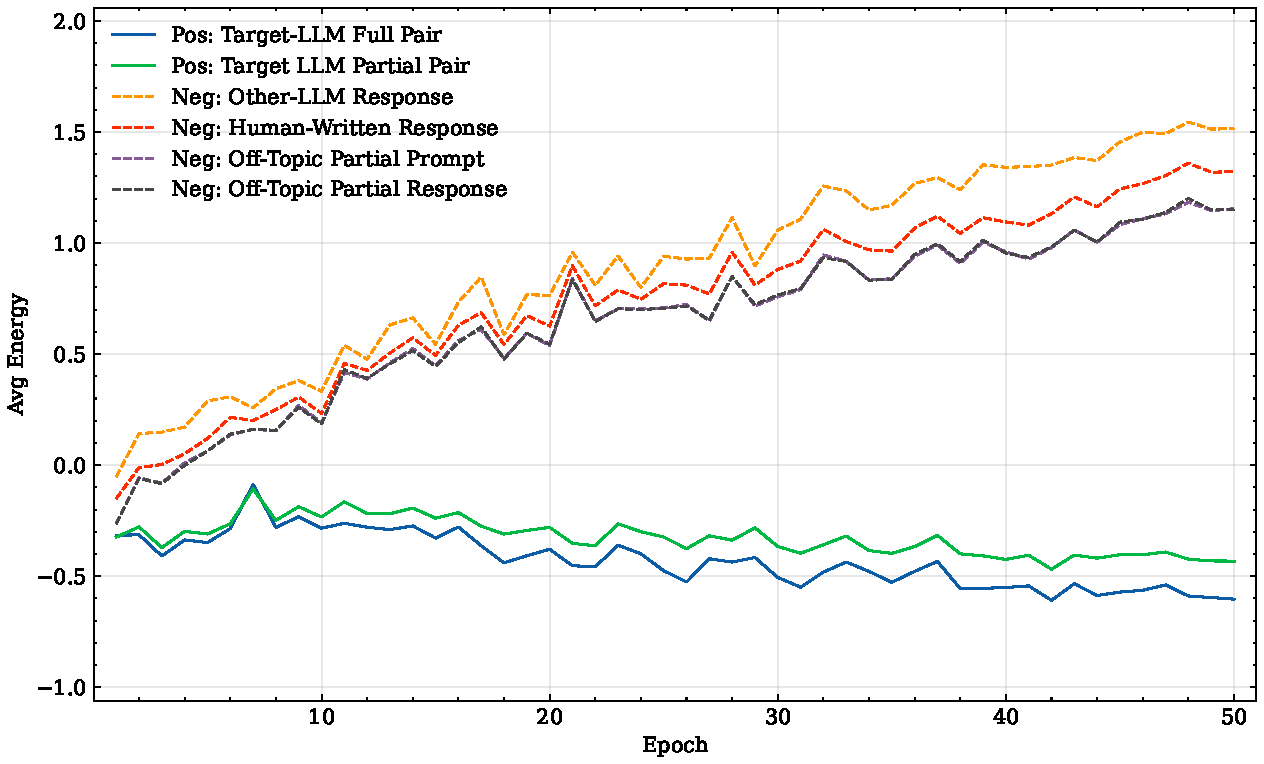
\includegraphics[width=0.48\textwidth]{figures/plot_ebm2s4cwiki_hyb_pretraining_energy.pdf}
    }
    \hfill
    \subfigure[توزیع انرژی در $\mathcal{E}_{\text{\lr{hybrid}}}^{\text{\lr{210M}}}$]{\label{fig:chap5_capacity_energy_210m}
        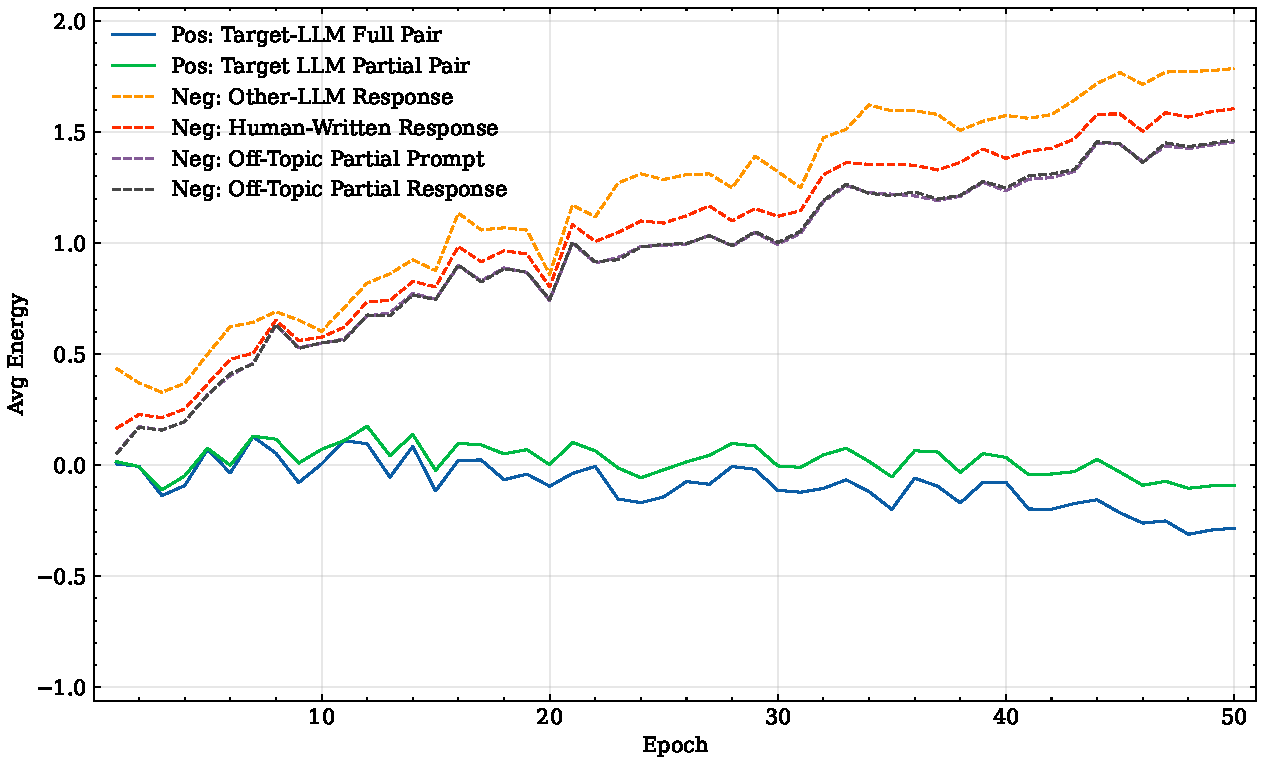
\includegraphics[width=0.48\textwidth]{figures/plot_ebm2s10cwiki_hyb_pretraining_energy.pdf}
    }
    \vspace{-0.25cm}
    \caption{مقایسه‌ی توزیع انرژی اعتبارسنجی در مدل‌های ۱۶۷ و ۲۱۰ میلیون پارامتری}\label{fig:chap5_capacity_energy}
\end{figure}
\vspace{-0.75cm}
\begin{figure}[!ht]
    \centering
    \subfigure[روند خطا در $\mathcal{E}_{\text{\lr{hybrid}}}^{\text{\lr{167M}}}$]{\label{fig:chap5_capacity_loss_167m}
        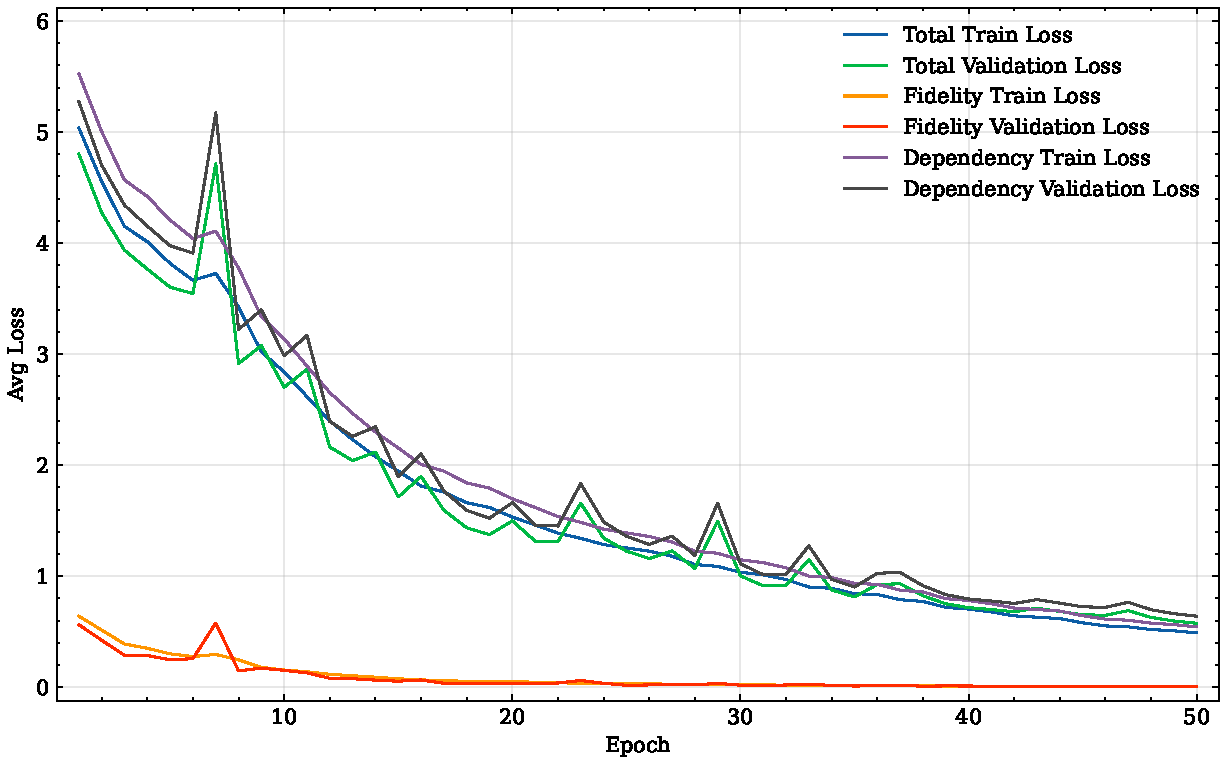
\includegraphics[width=0.48\textwidth]{figures/plot_ebm2s4cwiki_hyb_pretraining_loss.pdf}
    }
    \hfill
    \subfigure[روند خطا در $\mathcal{E}_{\text{\lr{hybrid}}}^{\text{\lr{210M}}}$]{\label{fig:chap5_capacity_loss_210m}
        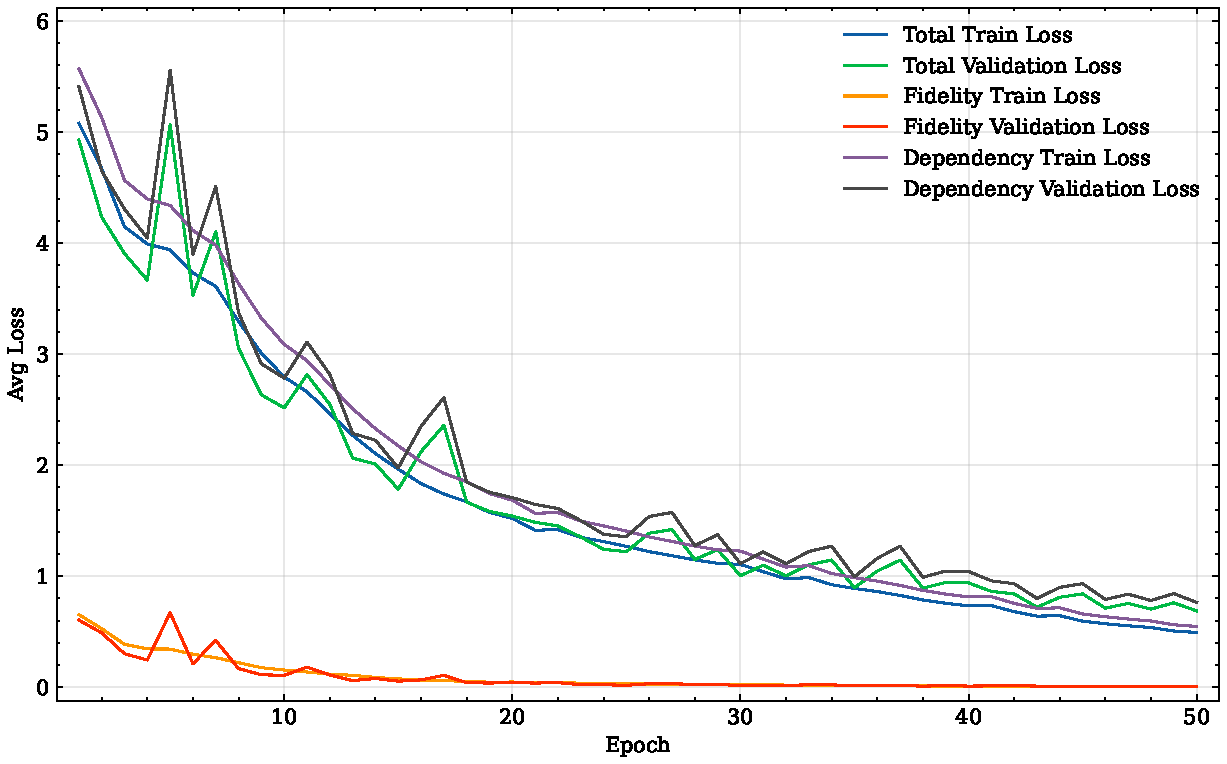
\includegraphics[width=0.48\textwidth]{figures/plot_ebm2s10cwiki_hyb_pretraining_loss.pdf}
    }
    \vspace{-0.25cm}
    \caption{مقایسه‌ی خطای آموزش و اعتبارسنجی در مدل‌های ۱۶۷ و ۲۱۰ میلیون پارامتری.}\label{fig:chap5_capacity_loss}
\end{figure}

نمودارهای توزیع انرژی (شکل~\ref{fig:chap5_capacity_energy}) نشان می‌دهد که در هر دو مدل، انرژی نمونه‌های مثبت به سمت مقادیر منفی سوق یافته و انرژی نمونه‌های منفی روندی افزایشی داشته است. تفاوت شکاف انرژی میان دو مدل ۱۶۷ و ۲۱۰ میلیون پارامتری نسبتاً محدود است که نشان می‌دهد برای پیچیدگی موجود در داده‌های به‌کار رفته، ظرفیت مدل ۱۶۷ میلیونی نیز کفایت بازنمایی لازم را فراهم می‌آورد. روند خطای اعتبارسنجی (شکل~\ref{fig:chap5_capacity_loss}) نیز هم‌گرایی پایدار هر دو مدل را پیش از اتمام ایپاک‌ها تأیید می‌کند.

\paragraph{پویایی توابع زیان و استراتژی‌های یادگیری.}
برای سنجش اثر مستقیم تابع زیان در ظرفیت ثابت، سه مدل ۱۸۱ میلیون پارامتری با توابع زیان وفاداری مطلق ($\mathcal{E}_{\text{\lr{fidelity}}}^{\text{\lr{181M}}}$)، وابستگی محلی مطلق ($\mathcal{E}_{\text{\lr{dependency}}}^{\text{\lr{181M}}}$) و ترکیبی ($\mathcal{E}_{\text{\lr{hybrid}}}^{\text{\lr{181M}}}$) بر روی مجموعه‌داده‌ی \lr{HC3} آموزش داده شدند.

توزیع انرژی و روند خطای این سه مدل در شکل‌های~\ref{fig:chap5_loss_energy} و~\ref{fig:chap5_loss_convergence} مقایسه شده است.

\begin{figure}[!ht]
    \centering
    \subfigure[انرژی در $\mathcal{E}_{\text{\lr{fidelity}}}^{\text{\lr{181M}}}$]{\label{fig:chap5_loss_energy_fid}
        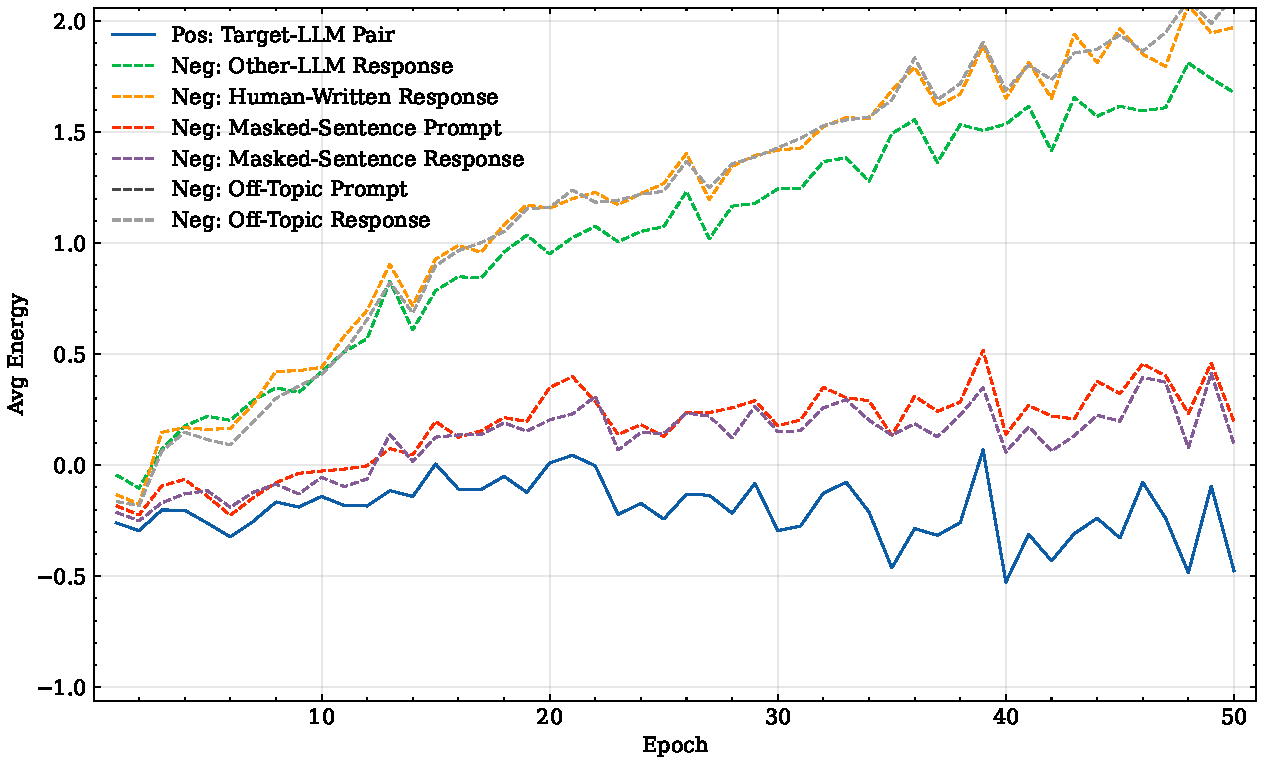
\includegraphics[width=0.31\textwidth]{figures/plot_ebm2s6chc3_fid_pretraining_energy.pdf}
    }%
    \hfill
    \subfigure[انرژی در $\mathcal{E}_{\text{\lr{dependency}}}^{\text{\lr{181M}}}$]{\label{fig:chap5_loss_energy_dep}
        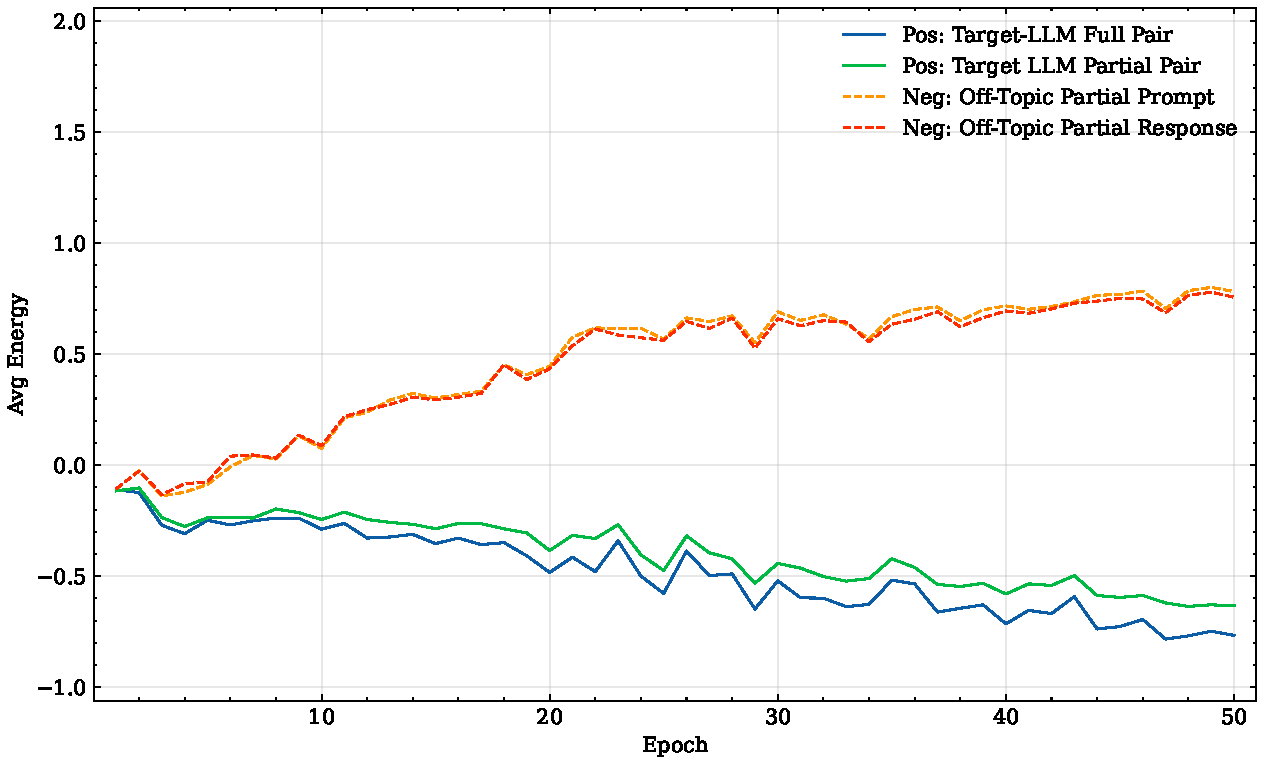
\includegraphics[width=0.31\textwidth]{figures/plot_ebm2s6chc3_dep_pretraining_energy.pdf}
    }%
    \hfill
    \subfigure[انرژی در $\mathcal{E}_{\text{\lr{hybrid}}}^{\text{\lr{181M}}}$]{\label{fig:chap5_loss_energy_hyb}
        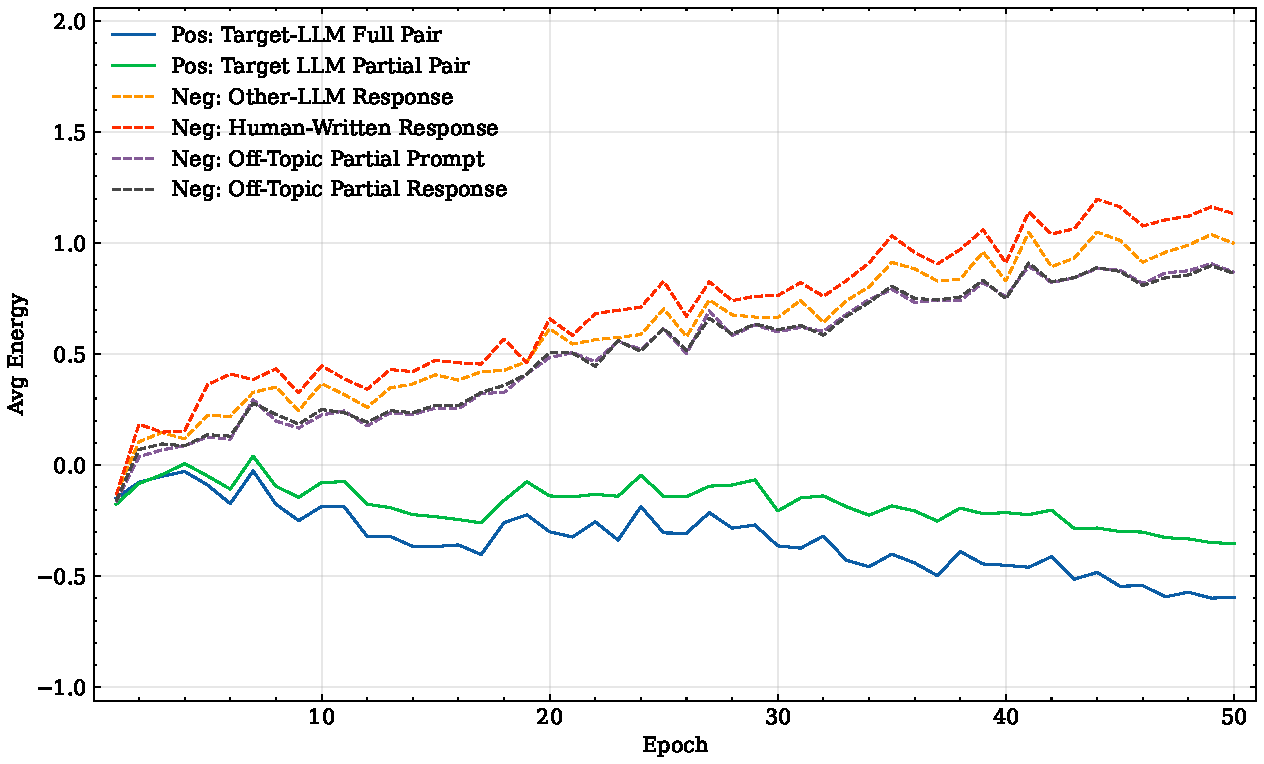
\includegraphics[width=0.31\textwidth]{figures/plot_ebm2s6chc3_hyb_pretraining_energy.pdf}
    }
    \vspace{-0.25cm}
    \caption{مقایسه‌ی توزیع انرژی اعتبارسنجی تحت سه استراتژی یادگیری متفاوت}\label{fig:chap5_loss_energy}
\end{figure}

\begin{figure}[!ht]
    \centering
    \subfigure[خطا در $\mathcal{E}_{\text{\lr{fidelity}}}^{\text{\lr{181M}}}$]{\label{fig:chap5_loss_fid}
        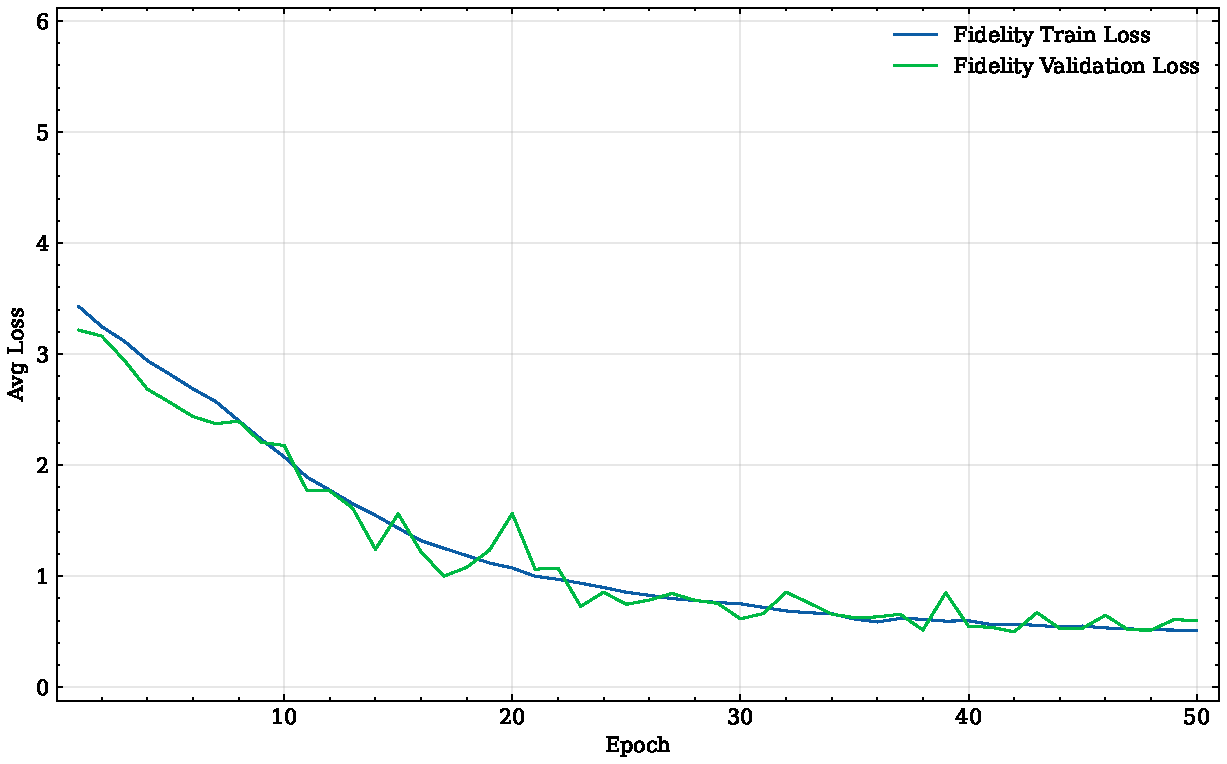
\includegraphics[width=0.31\textwidth]{figures/plot_ebm2s6chc3_fid_pretraining_loss.pdf}
    }%
    \hfill
    \subfigure[خطا در $\mathcal{E}_{\text{\lr{dependency}}}^{\text{\lr{181M}}}$]{\label{fig:chap5_loss_dep}
        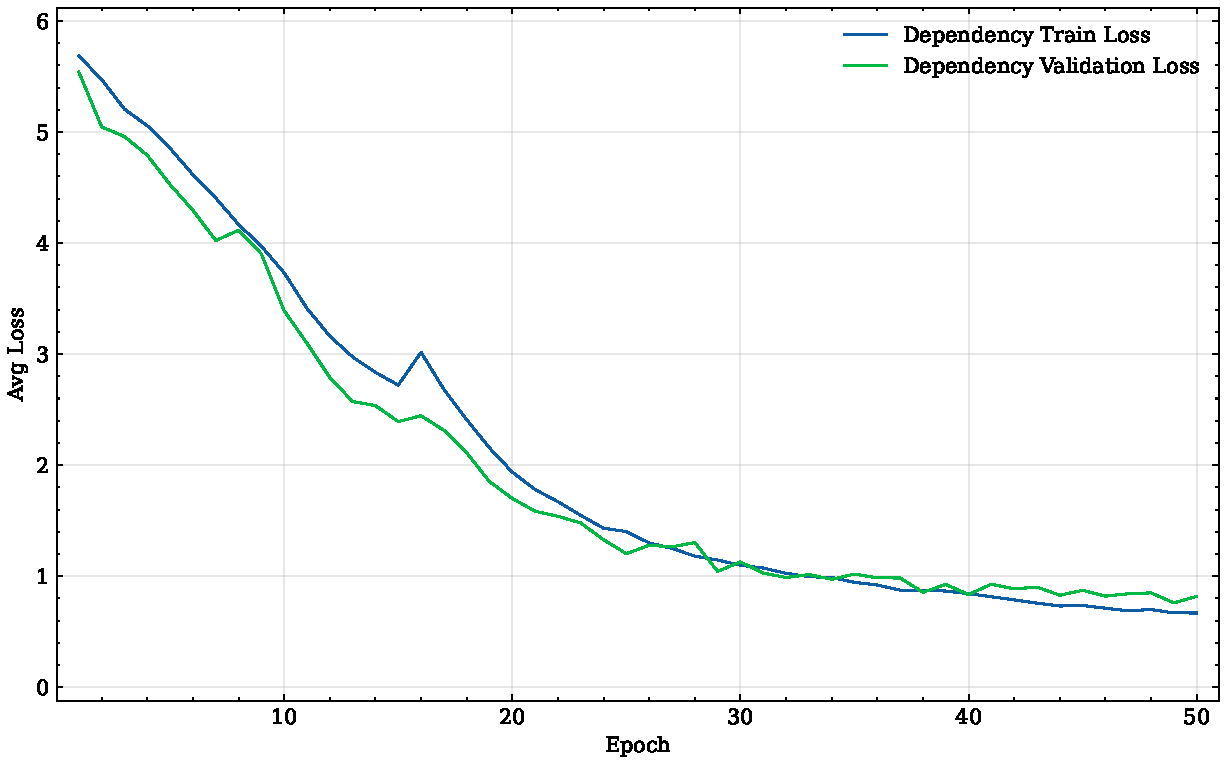
\includegraphics[width=0.31\textwidth]{figures/plot_ebm2s6chc3_dep_pretraining_loss.pdf}
    }%
    \hfill
    \subfigure[خطا در $\mathcal{E}_{\text{\lr{hybrid}}}^{\text{\lr{181M}}}$]{\label{fig:chap5_loss_hyb}
        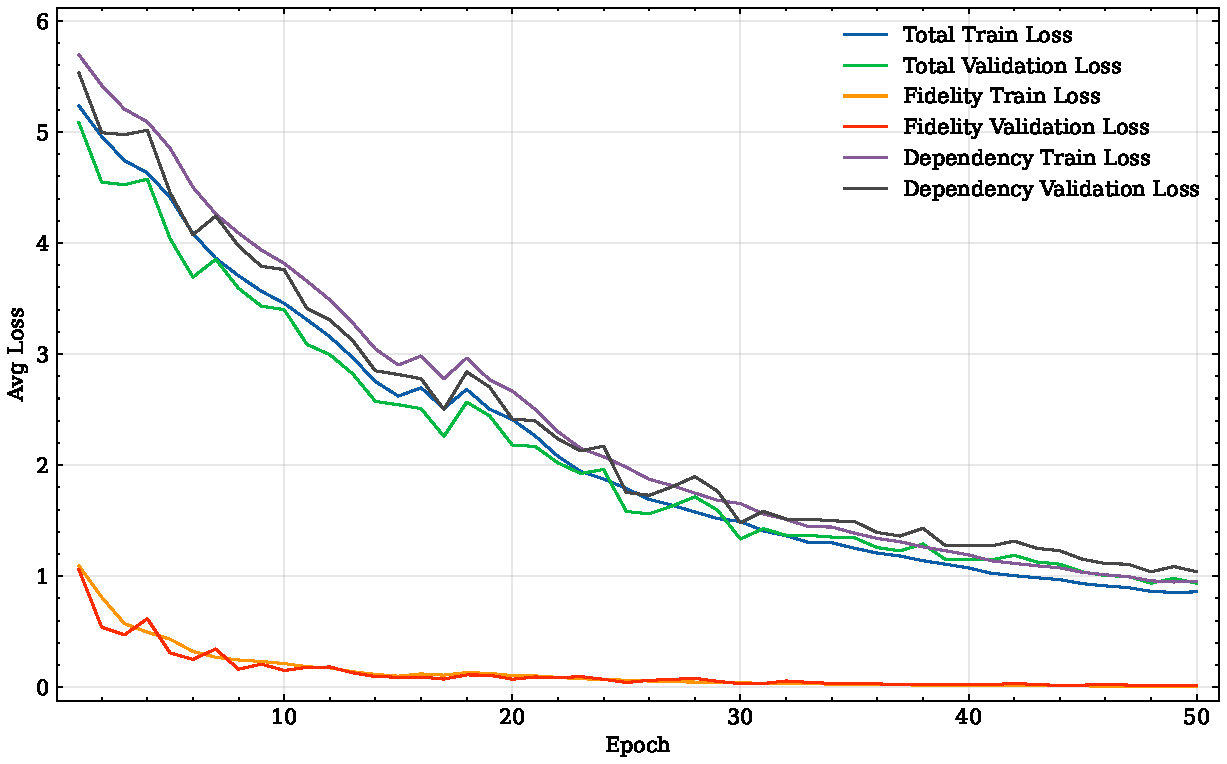
\includegraphics[width=0.31\textwidth]{figures/plot_ebm2s6chc3_hyb_pretraining_loss.pdf}
    }
    \vspace{-0.25cm}
    \caption{مقایسه‌ی خطای آموزش و اعتبارسنجی در سه پیکربندی تابع زیان.}\label{fig:chap5_loss_convergence}
\end{figure}

در شکل~\ref{fig:chap5_loss_energy_fid}، مدل $\mathcal{E}_{\text{\lr{fidelity}}}^{\text{\lr{181M}}}$ شکاف عریضی میان نمونه‌های مثبت و منفی ایجاد کرده است؛ اما همان‌گونه که در تحلیل بخش~\ref{sec:5-2-2} نشان داده شد، بخشی از این تفکیک ناشی از اتکا به آرتیفکت‌های قالبی است. در شکل~\ref{fig:chap5_loss_energy_dep}، مدل $\mathcal{E}_{\text{\lr{dependency}}}^{\text{\lr{181M}}}$ نوسانات کمتری دارد اما شکاف بسته‌تری ایجاد می‌کند. سرانجام، مدل ترکیبی پیشنهادی $\mathcal{E}_{\text{\lr{hybrid}}}^{\text{\lr{181M}}}$ (شکل~\ref{fig:chap5_loss_energy_hyb})، روندی باثبات‌تر ارائه کرده و تعادل مطلوبی میان تفکیک موضعی و پایداری سراسری خمینه‌ی انرژی نشان می‌دهد.


\subsection{تحلیل عملکرد پایین‌دست انرژی بر یادگیری مفسر}\label{sec:5-2-4}

در چارچوب \lr{ESCI}، شبکه‌ی انرژی نقش ارزیاب و منتقد را ایفا می‌کند تا گرادیان‌های لازم را برای آموزش شبکه‌ی مفسر ($\mathcal{IN}$) فراهم آورد. بنابراین، بررسی نحوه‌ی هدایت مفسر توسط مدل‌های انرژی، معیاری کلیدی برای اعتبارسنجی منتقد است.

ارزیابی‌ها نشان داد که مفسر هدایت‌شده توسط مدل وفاداری مطلق ($\mathcal{E}_{\text{\lr{fidelity}}}^{\text{\lr{181M}}}$)، به‌دلیل عدم‌حساسیت منتقد به وابستگی‌های موضعی، ماسک‌هایی مسطح و با خلوتی ناکافی تولید می‌کند. مقایسه‌ی رفتار آموزشی مفسر تحت نظارت دو منتقد دیگر یعنی مدل وابستگی مطلق ($\mathcal{IN}_{\text{\lr{dependency}}}^{\text{\lr{180M}}}$ هدایت‌شده توسط $\mathcal{E}_{\text{\lr{dependency}}}^{\text{\lr{181M}}}$) و مدل ترکیبی ($\mathcal{IN}_{\text{\lr{hybrid}}}^{\text{\lr{180M}}}$ هدایت‌شده توسط $\mathcal{E}_{\text{\lr{hybrid}}}^{\text{\lr{181M}}}$) در شکل~\ref{fig:chap5_interpreter_loss} ترسیم شده است.

\vspace{0.4cm}
\begin{figure}[!ht]
    \centering
    \subfigure[روند خطای مفسر $\mathcal{IN}_{\text{\lr{dependency}}}^{\text{\lr{180M}}}$]{\label{fig:chap5_interpreter_dep_loss}
        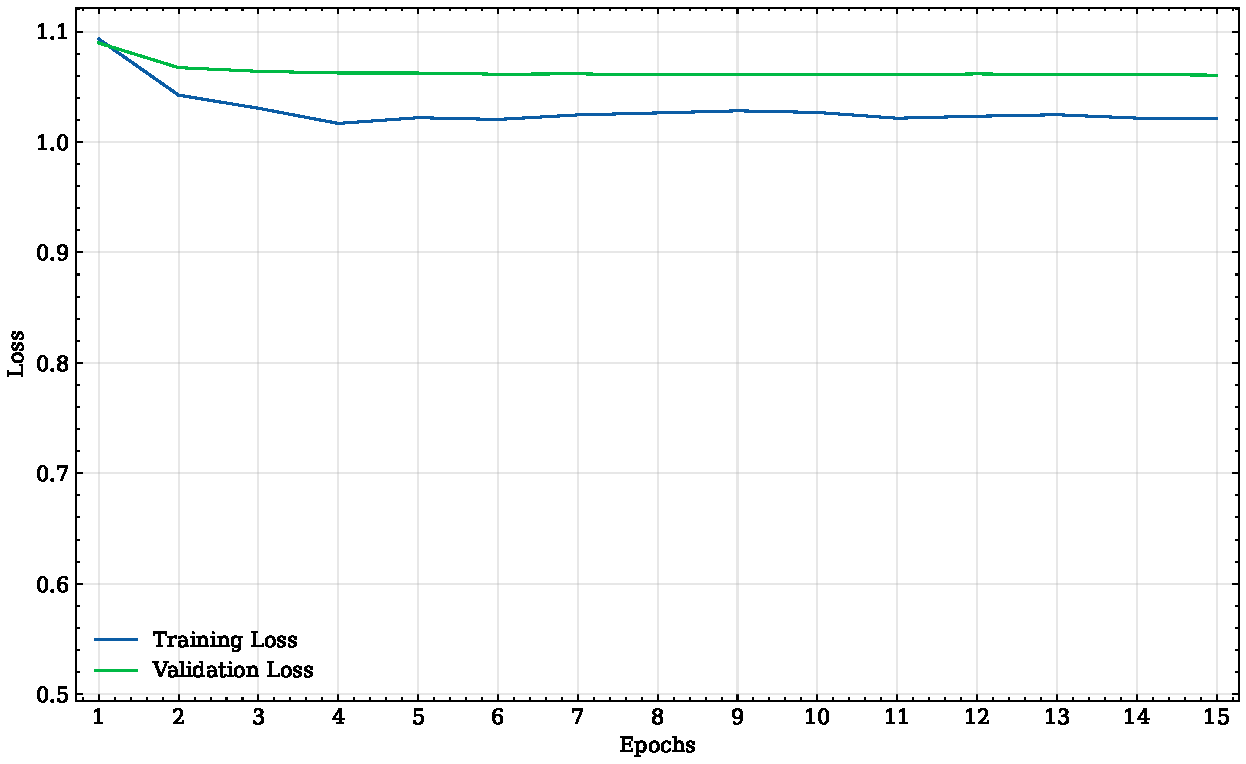
\includegraphics[width=0.48\textwidth]{figures/plot_interpreter1_loss.pdf}
    }
    \hfill
    \subfigure[روند خطای مفسر $\mathcal{IN}_{\text{\lr{hybrid}}}^{\text{\lr{180M}}}$]{\label{fig:chap5_interpreter_hyb_loss}
        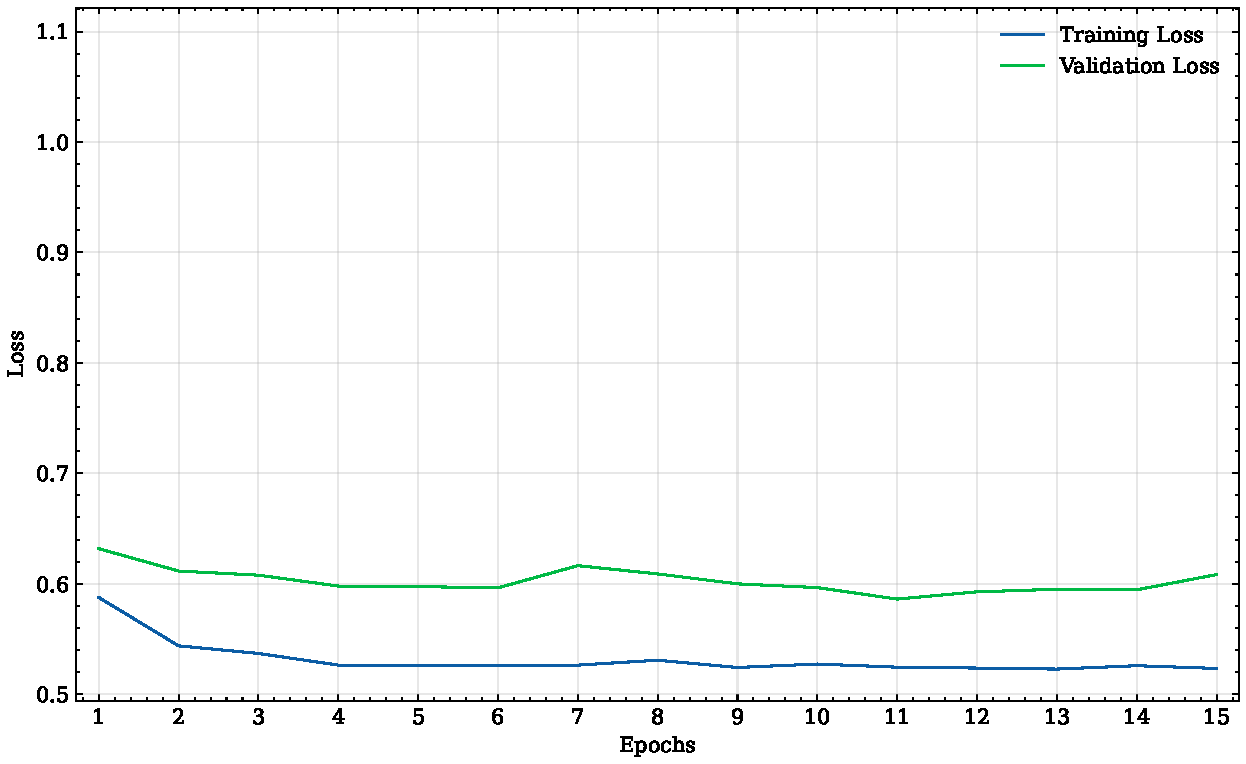
\includegraphics[width=0.48\textwidth]{figures/plot_interpreter2_loss.pdf}
    }
    \vspace{-0.25cm}
    \caption{مقایسه‌ی یادگیری شبکه‌ی مفسر تحت هدایت دو مدل انرژی متفاوت}\label{fig:chap5_interpreter_loss}
\end{figure}
\vspace{0.25cm}

همان‌طور که در شکل~\ref{fig:chap5_interpreter_dep_loss} مشاهده می‌شود، مفسر تحت هدایت $\mathcal{E}_{\text{\lr{dependency}}}$ روند هم‌گرایی کندی داشته و خطای اعتبارسنجی در محدوده‌ی بالای $1.06$ متوقف می‌گردد. در غیاب منظم‌سازی سراسری، خمینه‌ی انرژی در قبال ماسک‌های نرم مفسر، حساسیت شدیدی نشان داده و گرادیان‌هایی با نوسان و ناپایداری بالا تولید می‌کند که بهینه‌سازی مفسر را با دشواری روبه‌رو می‌سازد.

در مقابل، در نمودار ب (شکل~\ref{fig:chap5_interpreter_hyb_loss})، مفسر تحت هدایت مدل ترکیبی $\mathcal{IN}_{\text{\lr{hybrid}}}^{\text{\lr{180M}}}$، کاهش منظم خطا تا محدوده‌ی $0.59$ را تجربه می‌کند. مؤلفه‌ی وفاداری سراسری در تابع زیان منتقد، فضای انرژی را هموارتر ساخته و گرادیان‌های باثبات‌تری برای هدایت مفسر فراهم می‌آورد. این تحلیل تأیید می‌کند که مدل انرژی بهینه باید هم‌زمان از حاشیه‌ی تفکیک موضعی و منظم‌سازی سراسری برخوردار باشد تا یادگیری مفسر به‌صورت پایدار محقق گردد.


\section{ارزیابی مفسر در محیط‌های با دسترسی متفاوت}\label{sec:5-3}

پس از بررسی ویژگی‌های شبکه‌ی جانشین انرژی، این بخش به ارزیابی عملکرد سیستم یکپارچه، یعنی شبکه‌ی مفسر (\lr{ESCI}) می‌پردازد. هدف مفسر، استخراج زیرمجموعه‌ای خلوت از جملات پرامپت است که به‌عنوان پیش‌نیازهای گزاره‌ای در تولید خروجی نقش داشته‌اند. با توجه به چالش‌های ارزیابی در مدل‌های زبانی بزرگ، این بررسی در سه فاز ساختاردهی شده است: نخست، معقولیت انتساب که هم‌خوانی استخراج‌ها را با داوران زبانی و حقایق ساختاریافته می‌سنجد؛ دوم، وفاداری تجربی (شامل معیارهای جامعیت و کفایت) که از طریق مداخله در ورودی، میزان تأثیر گزاره‌های منتخب را می‌سنجد؛ و سوم، بررسی کیفی که نمونه‌های موردی را تحلیل می‌نماید.


\subsection{معقولیت انتساب}\label{sec:5-3-1}

پیش از سنجش پرهزینه‌ی تغییرات عملکردی مدل از طریق مداخله، می‌توان ابتدا معقولیت انتساب را ارزیابی کرد. این ارزیابی بررسی می‌کند که آیا جملات انتخاب‌شده توسط مفسر \lr{ESCI}، از نظر زبان‌شناختی و منطق مفهومی، پیش‌آیند معقولی برای خروجی هدف محسوب می‌شوند یا خیر. 

برای سنجش این مؤلفه، ارزیابی در دو ساختار متمایز انجام می‌پذیرد: نخست در محیط تولید متن آزاد در برابر هیئت اوراکل‌های زبانی (مجموعه‌داده‌ی \lr{HC3})، و سپس در محیط استدلال مقید مبتنی بر داده در برابر شبه‌حقیقت پایه‌ی استخراجی (مجموعه‌داده‌ی \lr{WikiBio}). پیش از بررسی نتایج، ابتدا معیارهای محاسباتی فرمول‌بندی می‌شوند.

\paragraph{فرمول‌بندی معیارهای ارزیابی کمّی.}
از آنجا که خروجی روش‌های مختلف از نظر مقیاس متفاوت است، تمامی خروجی‌ها پیش از ارزیابی نرمال‌سازی شده و مقادیر منفی (در صورت وجود در خروجی برخی روش‌های پایه‌ی کلاسیک) به صفر برش می‌خورند تا مجموع امتیازات اهمیت برای جملات هر پرامپت برابر با $1.0$ گردد. 

مطابق با تعاریف ارائه‌شده در فصل~\ref{chap:chapter1_introduction}، فرض کنید پرامپت ورودی شامل $N$ جمله به‌صورت مذکور یعنی $\mathbf{x} = (x_1, \dots, x_N) \in \mathcal{S}^N$ باشد. بردار $\mathbf{s}_{\text{\lr{ref}}} \in \mathbb{R}^N$ نشان‌دهنده‌ی امتیازات اهمیت در مدل مرجع (حقیقت پایه یا اوراکل)، و بردار $\mathbf{s}_{\text{\lr{pred}}} \in \mathbb{R}^N$ نمایانگر امتیازات پیش‌بینی‌شده توسط مفسر برای گزاره‌های پرامپت است. چنانچه مفسری به‌دلیل ناپایداری آموزش، امتیازات کاملاً یکنواختی به تمامی جملات پرامپت اختصاص دهد (واریانس نزدیک به صفر)، معیارهای آن صفر در نظر گرفته می‌شوند. عملکرد از طریق دو معیار زیر سنجیده می‌شود:

\begin{enumerate}
    \item \textbf{دقت برتر نرم (\lr{SoftAcc}):} از آنجا که در زبان طبیعی ممکن است چندین جمله‌ی مکمل برای پشتیبانی از یک گزاره وجود داشته باشند، تطابق صرفاً بر مبنای تک‌انتخاب اول معیاری بسیار سخت‌گیرانه است. لذا معیار دقت برتر نرم را به‌گونه‌ای تعریف می‌کنیم که بررسی کند آیا جمله‌ی برتر انتخاب‌شده توسط مفسر، درون فهرست اولویت‌های برتر مرجع قرار دارد یا خیر.
    
    از نظر ریاضی، در تعریف این معیار ابتدا اندیس جمله‌ی با بالاترین امتیاز در مفسر مشخص می‌شود: $i^* = \operatorname*{argmax}_{i \in {\{1,\dots,N\}}} {(\mathbf{s}_{\text{\lr{pred}}})}_i$. سپس اگر $s_{\text{\lr{top2}}}$ دومین مقدار بزرگ و یکتا در توزیع مرجع $\mathbf{s}_{\text{\lr{ref}}}$ باشد، دقت نرم به‌صورت زیر تعریف می‌گردد:
    \begin{equation}
        \text{\lr{SoftAcc}} = \mathbb{I}\left[ {(\mathbf{s}_{\text{\lr{ref}}})}_{i^*} \ge s_{\text{\lr{top2}}} \right]
    \end{equation}
    این فرمول‌بندی تضمین می‌کند که اگر مرجع امتیاز یکسانی به دو جمله‌ی کلیدی داده باشد، انتخاب هر یک از آن‌ها توسط مفسر صحیح تلقی گردد.

    \item \textbf{بهره‌ی تجمعی تنزیل‌یافته‌ی نرمال‌شده (\lr{nDCG}):} این معیار کیفیت کل فهرست اولویت‌بندی‌شده توسط مفسر را در قیاس با مرجع داوری می‌کند~\cite{jarvelin2002cumulated}.
    اگر $\pi$ جایگشتی از اندیس‌ها باشد که امتیازات مفسر ($\mathbf{s}_{\text{\lr{pred}}}$) را به‌صورت نزولی مرتب می‌کند (به‌گونه‌ای که $\pi(1)$ اندیس مهم‌ترین جمله از دید مفسر باشد)، بهره‌ی تجمعی (\lr{DCG}) با استفاده از امتیازات مرجع به‌عنوان ارزش واقعی، به‌صورت زیر محاسبه می‌شود:
    \begin{equation}
        \text{\lr{DCG}} = \sum_{j=1}^{N} \frac{{(\mathbf{s}_{\text{\lr{ref}}})}_{\pi(j)}}{\log_2(j+1)}
    \end{equation}
    با تقسیم این مقدار بر بهره‌ی ایده‌آل (\lr{IDCG}) که در آن مرتب‌سازی مستقیماً بر اساس مقادیر نزولی خود $\mathbf{s}_{\text{\lr{ref}}}$ انجام می‌شود، نمره‌ی نرمال‌شده‌ی \lr{nDCG} در بازه‌ی $[0, 1]$ به‌دست می‌آید.
\end{enumerate}

\paragraph{تفسیر ماتریس‌های مقایسه‌ای متقاطع.}
نتایج در قالب ماتریس‌های مقایسه‌ای متقاطع مربعی (با ابعاد متناظر با تعداد مدل‌های مورد ارزیابی) گزارش می‌شوند که در آن‌ها \textbf{سطرها نشان‌دهنده‌ی مدل مفسر (پیش‌بینی‌کننده)} و \textbf{ستون‌ها نشان‌دهنده‌ی مدل مرجع (داور)} می‌باشند.

به بیان دیگر، درایه‌ی واقع در سطر $A$ و ستون $B$ نشان می‌دهد که در صورت فرض مدل $B$ به‌عنوان مرجع، خروجی‌های مدل $A$ تا چه اندازه با آن منطبق است. قطر اصلی این ماتریس‌ها عدد $1.000$ را نشان می‌دهد. تفاوت مقدار درایه‌ی $A,B$ با $B,A$ ناشی از تفاوت توزیع خروجی مدل‌ها (برای مثال، پراکندگی در برابر خلوتی، یا نامتقارن بودن تعریف دقت برتر نرم) است.


\subsubsection{عملکرد روی مجموعه‌داده‌ی \lr{HC3}}\label{sec:5-3-1-1}

همان‌طور که پیش‌تر اشاره شد، در متون آزاد به‌دلیل فقدان برچسب‌های ازپیش‌تعیین‌شده، استفاده از مدل‌های زبانی پیشرفته به‌عنوان اوراکل می‌تواند تقریبی از معقولیت شناختی استخراج‌ها فراهم آورد.

\paragraph{تنظیمات آزمایش.}
مجموعه‌داده‌ی \lr{HC3} به مکالمات و پرسش و پاسخ‌های آزاد اختصاص دارد. برای شبیه‌سازی سناریوی مسدود، مدل تجاری \lr{GPT–4o–Mini} به‌عنوان مدل هدف انتخاب شده است و مفسر \lr{ESCI} بر روی پاسخ‌های این مدل ارزیابی می‌شود. ارزیابی معقولیت بر روی زیرمجموعه‌ای شامل ۲۰۰ جفت پرامپت-پاسخ (شامل حدود ۲۰۰۰ وظیفه‌ی انتساب جمله‌ای یکتا) در برابر هیئت اوراکل‌ها (شامل \lr{Gemini–2.5–Flash}، \lr{GPT–4o–Mini}، \lr{Gemma–2–9B–It}، \lr{Llama–3.1–8B–Instruct} و \lr{Mistral–7B–Instruct–v0.2}) انجام گرفته است. از اوراکل‌ها خواسته شد تا توزیع اهمیت گزاره‌ای جملات پرامپت را در قبال جمله‌ی هدف مشخص گزارش کنند.

\vspace{0.25cm}
\begin{table}[ht]
    \centering
    \footnotesize
    \caption{ماتریس‌های درهم‌ریختگی معقولیت انتساب، مجموعه‌داده‌ی \lr{HC3}}\label{tab:chap5_hc3_plausibility}
    \linespread{1}\selectfont
    \setlength{\tabcolsep}{3.5pt}
    \renewcommand{\arraystretch}{1.5}
    \setlength{\aboverulesep}{0pt}
    \setlength{\belowrulesep}{0pt}

    % --- TOP TABLE ---
    \textbf{(الف) معیار \lr{Soft Top-1 Accuracy}} \\[4pt]
    \begin{tabular}{l !{\color{black}\vline} c !{\color{black}\vline} c !{\color{gray!20}\vrule} c !{\color{gray!20}\vrule} c !{\color{gray!20}\vrule} c !{\color{gray!20}\vrule} c} % chktex 26
        \toprule
        \rowcolor{gray!15} \textbf{\lr{Ref $\leftarrow$ | Interpreter $\downarrow$}} &  \textbf{\lr{ESCI}} & \multicolumn{1}{!{\color{gray!15}\vrule}c}{\textbf{\lr{Gemini–2.5}}} & \multicolumn{1}{!{\color{gray!15}\vrule}c}{\textbf{\lr{GPT–4o–Mini}}} & \multicolumn{1}{!{\color{gray!15}\vrule}c}{\textbf{\lr{Gemma–2}}} & \multicolumn{1}{!{\color{gray!15}\vrule}c}{\textbf{\lr{Llama–3.1}}} & \multicolumn{1}{!{\color{gray!15}\vrule}c}{\textbf{\lr{Mistral–7B}}} \\
        \midrule
        \textbf{\lr{ESCI (Ours)}} & $\mathbf{1.000}$ & $0.750$ & $0.640$ & $0.700$ & $0.720$ & $0.740$ \\
        \midrule
        \lr{Gemini–2.5–Flash} & $0.670$ & $\mathbf{1.000}$ & $\mathbf{0.750}$ & $0.650$ & $0.680$ & $0.670$ \\
        \arrayrulecolor{gray!20}\midrule[0.1pt]
        \lr{GPT–4o–Mini} & $0.600$ & $\mathbf{0.850}$ & $\mathbf{1.000}$ & $0.620$ & $0.640$ & $0.650$ \\
        \arrayrulecolor{gray!20}\midrule[0.1pt]
        \lr{Gemma–2–9B–It} & $0.690$ & $0.650$ & $0.490$ & $\mathbf{1.000}$ & $\mathbf{0.830}$ & $0.780$ \\
        \arrayrulecolor{gray!20}\midrule[0.1pt]
        \lr{Llama–3.1–8B–It} & $\mathbf{0.720}$ & $0.680$ & $0.510$ & $\mathbf{0.850}$ & $\mathbf{1.000}$ & $\mathbf{0.800}$ \\
        \arrayrulecolor{gray!20}\midrule[0.1pt]
        \lr{Mistral–7B–It} & $0.700$ & $0.670$ & $0.520$ & $0.790$ & $0.810$ & $\mathbf{1.000}$ \\
        \arrayrulecolor{black}\bottomrule
    \end{tabular}

    \vspace{0.25cm}

    % --- BOTTOM TABLE ---
    \textbf{(ب) معیار \lr{nDCG}} \\[4pt]
    \begin{tabular}{l !{\color{black}\vline} c !{\color{black}\vline} c !{\color{gray!20}\vrule} c !{\color{gray!20}\vrule} c !{\color{gray!20}\vrule} c !{\color{gray!20}\vrule} c} % chktex 26
        \toprule
        \rowcolor{gray!15} \textbf{\lr{Ref $\leftarrow$ | Interpreter $\downarrow$}} & \textbf{\lr{ESCI}} & \multicolumn{1}{!{\color{gray!15}\vrule}c}{\textbf{\lr{Gemini–2.5}}} & \multicolumn{1}{!{\color{gray!15}\vrule}c}{\textbf{\lr{GPT–4o–Mini}}} & \multicolumn{1}{!{\color{gray!15}\vrule}c}{\textbf{\lr{Gemma–2}}} & \multicolumn{1}{!{\color{gray!15}\vrule}c}{\textbf{\lr{Llama–3.1}}} & \multicolumn{1}{!{\color{gray!15}\vrule}c}{\textbf{\lr{Mistral–7B}}} \\
        \midrule
        \textbf{\lr{ESCI (Ours)}} & $\mathbf{1.000}$ & $0.830$ & $0.790$ & $0.810$ & $0.820$ & $0.830$ \\
        \midrule
        \lr{Gemini–2.5–Flash} & $\mathbf{0.850}$ & $\mathbf{1.000}$ & $\mathbf{0.880}$ & $0.760$ & $0.780$ & $0.790$ \\
        \arrayrulecolor{gray!20}\midrule[0.1pt]
        \lr{GPT–4o–Mini} & $0.770$ & $\mathbf{0.890}$ & $\mathbf{1.000}$ & $0.770$ & $0.790$ & $0.800$ \\
        \arrayrulecolor{gray!20}\midrule[0.1pt]
        \lr{Gemma–2–9B–It} & $0.800$ & $0.750$ & $0.740$ & $\mathbf{1.000}$ & $\mathbf{0.860}$ & $0.830$ \\
        \arrayrulecolor{gray!20}\midrule[0.1pt]
        \lr{Llama–3.1–8B–It} & $0.820$ & $0.770$ & $0.750$ & $\mathbf{0.880}$ & $\mathbf{1.000}$ & $\mathbf{0.850}$ \\
        \arrayrulecolor{gray!20}\midrule[0.1pt]
        \lr{Mistral–7B–It} & $0.810$ & $0.780$ & $0.760$ & $0.820$ & $0.840$ & $\mathbf{1.000}$ \\
        \arrayrulecolor{black}\bottomrule
    \end{tabular}
\end{table}
\vspace{-0.25cm}

\paragraph{تحلیل و مقایسه.}
جدول~\ref{tab:chap5_hc3_plausibility} نتایج ارزیابی معقولیت را برای اوراکل‌ها و مفسر \lr{ESCI} نشان می‌دهد. نتایج حاکی از آن است که مفسر \lr{ESCI} با ساختار سبک خود، به هم‌ترازی بالایی با داوری اوراکل‌های زبانی در انتخاب جملات کلیدی دست یافته است. هنگامی که \lr{ESCI} در نقش مفسر (سطر اول جدول الف) قرار می‌گیرد، تک‌انتخاب برتر آن در $75\%$ مواقع با قضاوت \lr{Gemini-2.5}، در $72\%$ مواقع با \lr{Llama-3.1} و در $74\%$ مواقع با قضاوت \lr{Mistral-7B} هم‌خوانی دارد. این هم‌ترازی در معیار \lr{nDCG} (جدول ب) نیز با کسب امتیازات بالای $0.80$ برای اکثر مدل‌ها تکرار می‌شود و نشان می‌دهد که مدل جانشین توانسته است توزیع اهمیت جملات را به‌شکل مؤثری تقریب بزند.

تفاوت ارقام سطر اول با ستون اول، ناشی از تفاوت رفتار مفسرهاست. اوراکل‌های مولد عموماً مقادیر وزن را به‌صورت گسترده‌تری میان جملات پرامپت پخش می‌کنند؛ در حالی که مفسر \lr{ESCI} به‌دلیل بهره‌گیری از جریمه‌ی پراکندگی $L_1$ در آموزش، ماسک‌هایی خلوت‌تر تولید می‌کند. در نتیجه، انتخاب‌های خلوت \lr{ESCI} غالباً در دامنه‌ی گزینه‌های محتمل اوراکل‌ها قرار می‌گیرد.


\subsubsection{عملکرد روی مجموعه‌داده‌ی \lr{WikiBio}}\label{sec:5-3-1-2}

برای ارزیابی در محیطی مقید با لنگرگاه ساختاریافته، در این بخش عملکرد مفسر بر روی مجموعه‌داده‌ی \lr{WikiBio} سنجیده می‌شود که در آن علاوه بر داوری اوراکل‌ها، خط‌پایه‌ی مکاشفه‌ای تطبیق رشته‌ای (\lr{StringMatching}) نیز به‌عنوان شبه‌حقیقت پایه در دسترس است.

\paragraph{تنظیمات آزمایش.}
پیرو مباحث بخش~\ref{sec:5-1-2-2}، پاسخ‌های این مجموعه‌داده از روی جدول تولید می‌شوند. خط‌پایه‌ی تطبیق رشته‌ای (\lr{StringMatching}) بر مبنای اشتراک واژگانی میان جملات ورودی و خروجی عمل می‌کند. روش‌های مورد ارزیابی دو گروه می‌باشند: روش‌های جعبه‌سیاه (جدول~\ref{tab:chap5_wikibio_plausibility_blackbox}) و روش‌های دارای دسترسی ممتاز (جدول~\ref{tab:chap5_wikibio_plausibility_whitebox}) بر روی مدل هدف \lr{Llama–3.1–8B–It}.

\paragraph{معقولیت انتساب در روش‌های جعبه‌سیاه.}
جدول~\ref{tab:chap5_wikibio_plausibility_blackbox} نتایج را برای روش‌های جعبه‌سیاه نشان می‌دهد. ستون \lr{StringMatching} نقش خط‌پایه‌ی مرجع استخراجی را دارد. نتایج جدول الف نشان می‌دهد که مفسر \lr{ESCI} در $71.2\%$ مواقع، مهم‌ترین جمله‌ی استخراجی خود را با تطابق‌های لغوی موجود در جدول اطلاعات هم‌سو کرده است. نمره‌ی \lr{nDCG} معادل $0.637$ برای \lr{ESCI} در تقابل با این مبنای واژگانی، گویای آن است که خروجی‌های مفسر از معقولیت شناختی مناسبی برخوردارند.

از سوی دیگر، خط‌پایه‌ی \lr{LIME-BlackBox} انطباق $94.4\%$ با \lr{StringMatching} نشان می‌دهد. دلیل این امر، هم‌پوشانی متدولوژیک توابع هدف آن‌هاست؛ \lr{LIME-BlackBox} بر اساس معیار \lr{BERTScore} بهینه‌سازی می‌شود که شباهت واژگانی موضعی را اندازه می‌گیرد و لذا هم‌پوشانی بالایی با تطبیق رشته‌ای پیدا می‌کند. با این حال، همان‌طور که در بخش ارزیابی وفاداری (بخش~\ref{sec:5-3-2}) مشاهده خواهد شد، اشتراک واژگانی لزوماً به معنای شناسایی پیش‌آیندهای مؤثر در تولید متن نیست.

در تقابل مفسر پیشنهادی با هیئت اوراکل‌ها (ستون‌های پایانی جدول~\ref{tab:chap5_wikibio_plausibility_blackbox})، میزان انطباق مفسر با مدل‌هایی نظیر \lr{Gemma-2} و \lr{Llama-3.1} به محدوده‌ی $0.42$ تا $0.44$ می‌رسد و در تقابل با استفاده از \lr{Gemini-2.5-Flash} نیز در سطح $0.59$ است. این موضوع نشان‌دهنده‌ی یک گلوگاه ظرفیتی است؛ در وظیفه‌ی تولید متن از داده‌های جدولی، مدل‌های زبانی عظیم به‌دلیل ابعاد چند میلیارد پارامتری خود، نگاشت‌های دقیق کلید-مقدار را به‌آسانی تفکیک می‌کنند، در حالی که مفسر سبک‌وزن \lr{ESCI} با ۷۱ میلیون پارامتر آموزش‌پذیر، در این تفکیک‌های ریزدانه رفتاری محتاطانه‌تر به نمایش می‌گذارد.

\vspace{0.25cm}
\begin{table}[ht]
    \centering
    \footnotesize
    \caption{ماتریس‌های درهم‌ریختگی معقولیت انتساب، مجموعه‌داده‌ی \lr{WikiBio} (جعبه‌سیاه)}\label{tab:chap5_wikibio_plausibility_blackbox}
    \linespread{1}\selectfont
    \setlength{\tabcolsep}{7.5pt}
    \renewcommand{\arraystretch}{1.5}
    \setlength{\aboverulesep}{0pt}
    \setlength{\belowrulesep}{0pt}

    % --- TOP TABLE ---
    \textbf{(الف) معیار \lr{Soft Top-1 Accuracy}} \\[4pt]
    \begin{tabular}{l !{\color{black}\vline} c !{\color{black}\vline} c !{\color{gray!20}\vrule} c !{\color{gray!20}\vrule} c !{\color{gray!20}\vrule} c !{\color{gray!20}\vrule} c !{\color{gray!20}\vrule} c} % chktex 26
        \toprule
        \rowcolor{gray!15} \textbf{\lr{Ref $\leftarrow$ | Interp. $\downarrow$}} & \textbf{\lr{ESCI}} & \multicolumn{1}{!{\color{gray!15}\vrule}c}{\textbf{\lr{String}}} & \multicolumn{1}{!{\color{gray!15}\vrule}c}{\textbf{\lr{LIME-Blk}}} & \multicolumn{1}{!{\color{gray!15}\vrule}c}{\textbf{\lr{Gemini}}} & \multicolumn{1}{!{\color{gray!15}\vrule}c}{\textbf{\lr{Gemma}}} & \multicolumn{1}{!{\color{gray!15}\vrule}c}{\textbf{\lr{Llama}}} & \multicolumn{1}{!{\color{gray!15}\vrule}c}{\textbf{\lr{Mistral}}} \\
        \midrule
        \textbf{\lr{ESCI (Ours)}} & $\mathbf{1.000}$ & $0.712$ & $0.698$ & $0.591$ & $0.425$ & $0.439$ & $0.496$ \\
        \midrule
        \lr{StringMatching} & $\mathbf{0.991}$ & $\mathbf{1.000}$ & $\mathbf{1.000}$ & $\mathbf{0.880}$ & $\mathbf{0.992}$ & $\mathbf{0.956}$ & $\mathbf{0.981}$ \\
        \arrayrulecolor{gray!20}\midrule[0.1pt]
        \lr{LIME–BlackBox} & $0.395$ & $\mathbf{0.944}$ & $\mathbf{1.000}$ & $0.670$ & $0.524$ & $0.533$ & $0.422$ \\
        \arrayrulecolor{gray!20}\midrule[0.1pt]
        \lr{Gemini–2.5–Flash} & $0.359$ & $0.620$ & $0.610$ & $\mathbf{1.000}$ & $0.450$ & $0.460$ & $0.440$ \\
        \arrayrulecolor{gray!20}\midrule[0.1pt]
        \lr{Gemma–2–9B–It} & $0.362$ & $0.251$ & $0.369$ & $0.470$ & $\mathbf{1.000}$ & $0.791$ & $0.637$ \\
        \arrayrulecolor{gray!20}\midrule[0.1pt]
        \lr{Llama–3.1–8B–It} & $0.357$ & $0.321$ & $0.426$ & $0.480$ & $0.807$ & $\mathbf{1.000}$ & $0.640$ \\
        \arrayrulecolor{gray!20}\midrule[0.1pt]
        \lr{Mistral–7B–It} & $0.485$ & $0.337$ & $0.421$ & $0.450$ & $0.679$ & $0.675$ & $\mathbf{1.000}$ \\
        \arrayrulecolor{black}\bottomrule
    \end{tabular}

    \vspace{0.25cm}

    % --- BOTTOM TABLE ---
    \textbf{(ب) معیار \lr{nDCG}} \\[4pt]
    \begin{tabular}{l !{\color{black}\vline} c !{\color{black}\vline} c !{\color{gray!20}\vrule} c !{\color{gray!20}\vrule} c !{\color{gray!20}\vrule} c !{\color{gray!20}\vrule} c !{\color{gray!20}\vrule} c} % chktex 26
        \toprule
        \rowcolor{gray!15} \textbf{\lr{Ref $\leftarrow$ | Interp. $\downarrow$}} & \textbf{\lr{ESCI}} & \multicolumn{1}{!{\color{gray!15}\vrule}c}{\textbf{\lr{String}}} & \multicolumn{1}{!{\color{gray!15}\vrule}c}{\textbf{\lr{LIME-Blk}}} & \multicolumn{1}{!{\color{gray!15}\vrule}c}{\textbf{\lr{Gemini}}} & \multicolumn{1}{!{\color{gray!15}\vrule}c}{\textbf{\lr{Gemma}}} & \multicolumn{1}{!{\color{gray!15}\vrule}c}{\textbf{\lr{Llama}}} & \multicolumn{1}{!{\color{gray!15}\vrule}c}{\textbf{\lr{Mistral}}} \\
        \midrule
        \textbf{\lr{ESCI (Ours)}} & $\mathbf{1.000}$ & $0.637$ & $0.658$ & $0.621$ & $0.562$ & $0.569$ & $0.615$ \\
        \midrule
        \lr{StringMatching} & $\mathbf{0.741}$ & $\mathbf{1.000}$ & $\mathbf{0.915}$ & $\mathbf{0.860}$ & $\mathbf{0.811}$ & $\mathbf{0.819}$ & $\mathbf{0.765}$ \\
        \arrayrulecolor{gray!20}\midrule[0.1pt]
        \lr{LIME–BlackBox} & $0.646$ & $0.697$ & $\mathbf{1.000}$ & $0.660$ & $0.660$ & $0.676$ & $0.627$ \\
        \arrayrulecolor{gray!20}\midrule[0.1pt]
        \lr{Gemini–2.5–Flash} & $0.577$ & $\mathbf{0.701}$ & $0.687$ & $\mathbf{1.000}$ & $0.550$ & $0.560$ & $0.540$ \\
        \arrayrulecolor{gray!20}\midrule[0.1pt]
        \lr{Gemma–2–9B–It} & $0.493$ & $0.589$ & $0.652$ & $0.560$ & $\mathbf{1.000}$ & $0.805$ & $0.716$ \\
        \arrayrulecolor{gray!20}\midrule[0.1pt]
        \lr{Llama–3.1–8B–It} & $0.478$ & $0.565$ & $0.631$ & $0.570$ & $0.768$ & $\mathbf{1.000}$ & $0.673$ \\
        \arrayrulecolor{gray!20}\midrule[0.1pt]
        \lr{Mistral–7B–It} & $0.579$ & $0.586$ & $0.646$ & $0.550$ & $0.750$ & $0.741$ & $\mathbf{1.000}$ \\
        \arrayrulecolor{black}\bottomrule
    \end{tabular}
\end{table}
\vspace{-0.25cm}

\paragraph{معقولیت انتساب در روش‌های جعبه‌سفید و جعبه‌خاکستری.}
جدول~\ref{tab:chap5_wikibio_plausibility_whitebox} ماتریس‌های متناظر را برای روش‌های دارای دسترسی ممتاز (روش‌های جعبه‌سفید و جعبه‌خاکستری مذکور در بخش~\ref{sec:5-1-3-2}) بر روی مدل هدف \lr{Llama–3.1–8B–It} نشان می‌دهد تا بررسی شود مفسر جعبه‌سیاه \lr{ESCI} تا چه اندازه با روش‌های آگاه از ساختار درونی هم‌سو است.

\begin{table}[ht]
    \centering
    \footnotesize
    \caption{ماتریس‌های درهم‌ریختگی معقولیت انتساب، مجموعه‌داده‌ی \lr{WikiBio} (جعبه‌سفید)}\label{tab:chap5_wikibio_plausibility_whitebox} 
    \linespread{1}\selectfont
    \setlength{\tabcolsep}{6.5pt}
    \renewcommand{\arraystretch}{1.45}
    \setlength{\aboverulesep}{0pt}
    \setlength{\belowrulesep}{0pt}

    % --- TOP TABLE ---
    \textbf{(الف) معیار \lr{Soft Top-1 Accuracy}} \\[4pt]
    \begin{tabular}{l !{\color{black}\vline} c !{\color{black}\vline} c !{\color{gray!20}\vrule} c !{\color{gray!20}\vrule} c !{\color{gray!20}\vrule} c !{\color{gray!20}\vrule} c !{\color{gray!20}\vrule} c !{\color{gray!20}\vrule} c} % chktex 26
        \toprule
        \rowcolor{gray!15} \textbf{\lr{Ref $\leftarrow$ | Interp. $\downarrow$}} & \textbf{\lr{ESCI}} & \multicolumn{1}{!{\color{gray!15}\vrule}c}{\textbf{\lr{String}}} & \multicolumn{1}{!{\color{gray!15}\vrule}c}{\textbf{\lr{Attn.}}} & \multicolumn{1}{!{\color{gray!15}\vrule}c}{\textbf{\lr{Roll.}}} & \multicolumn{1}{!{\color{gray!15}\vrule}c}{\textbf{\lr{G-SHAP}}} & \multicolumn{1}{!{\color{gray!15}\vrule}c}{\textbf{\lr{Inp$\times$G}}} & \multicolumn{1}{!{\color{gray!15}\vrule}c}{\textbf{\lr{S-LOO}}} & \multicolumn{1}{!{\color{gray!15}\vrule}c}{\textbf{\lr{LIME}}} \\
        \midrule
        \textbf{\lr{ESCI (Ours)}} & $\mathbf{1.000}$ & $0.712$ & $0.613$ & $0.712$ & $0.461$ & $0.281$ & $0.581$ & $0.471$ \\
        \midrule
        \lr{StringMatching} & $\mathbf{0.991}$ & $\mathbf{1.000}$ & $\mathbf{1.000}$ & $\mathbf{1.000}$ & $\mathbf{1.000}$ & $\mathbf{1.000}$ & $\mathbf{1.000}$ & $\mathbf{1.000}$ \\
        \arrayrulecolor{gray!20}\midrule[0.1pt]
        \lr{Attention} & $0.665$ & $0.905$ & $\mathbf{1.000}$ & $0.909$ & $0.467$ & $0.286$ & $0.432$ & $0.373$ \\
        \arrayrulecolor{gray!20}\midrule[0.1pt]
        \lr{AttentionRollout} & $0.615$ & $\mathbf{0.996}$ & $0.755$ & $\mathbf{1.000}$ & $0.403$ & $0.310$ & $0.119$ & $0.118$ \\
        \arrayrulecolor{gray!20}\midrule[0.1pt]
        \lr{GradientSHAP} & $0.388$ & $0.346$ & $0.424$ & $0.349$ & $\mathbf{1.000}$ & $0.281$ & $0.488$ & $0.401$ \\
        \arrayrulecolor{gray!20}\midrule[0.1pt]
        \lr{Input$\times$Gradient} & $0.195$ & $0.159$ & $0.229$ & $0.161$ & $0.258$ & $\mathbf{1.000}$ & $0.251$ & $0.196$ \\
        \arrayrulecolor{gray!20}\midrule[0.1pt]
        \lr{SentenceLOO} & $0.263$ & $0.128$ & $0.319$ & $0.129$ & $0.409$ & $0.259$ & $\mathbf{1.000}$ & $0.631$ \\
        \arrayrulecolor{gray!20}\midrule[0.1pt]
        \lr{LIME–GrayBox} & $0.364$ & $0.168$ & $0.355$ & $0.167$ & $0.371$ & $0.205$ & $0.761$ & $\mathbf{1.000}$ \\
        \arrayrulecolor{black}\bottomrule
    \end{tabular}

    \vspace{0.25cm}

    % --- BOTTOM TABLE ---
    \textbf{(ب) معیار \lr{nDCG}} \\[4pt]
    \begin{tabular}{l !{\color{black}\vline} c !{\color{black}\vline} c !{\color{gray!20}\vrule} c !{\color{gray!20}\vrule} c !{\color{gray!20}\vrule} c !{\color{gray!20}\vrule} c !{\color{gray!20}\vrule} c !{\color{gray!20}\vrule} c} % chktex 26
        \toprule
        \rowcolor{gray!15} \textbf{\lr{Ref $\leftarrow$ | Interp. $\downarrow$}} & \textbf{\lr{ESCI}} & \multicolumn{1}{!{\color{gray!15}\vrule}c}{\textbf{\lr{String}}} & \multicolumn{1}{!{\color{gray!15}\vrule}c}{\textbf{\lr{Attn.}}} & \multicolumn{1}{!{\color{gray!15}\vrule}c}{\textbf{\lr{Roll.}}} & \multicolumn{1}{!{\color{gray!15}\vrule}c}{\textbf{\lr{G-SHAP}}} & \multicolumn{1}{!{\color{gray!15}\vrule}c}{\textbf{\lr{Inp$\times$G}}} & \multicolumn{1}{!{\color{gray!15}\vrule}c}{\textbf{\lr{S-LOO}}} & \multicolumn{1}{!{\color{gray!15}\vrule}c}{\textbf{\lr{LIME}}} \\
        \midrule
        \textbf{\lr{ESCI (Ours)}} & $\mathbf{1.000}$ & $0.637$ & $0.743$ & $0.726$ & $0.607$ & $0.508$ & $0.625$ & $0.624$ \\
        \midrule
        \lr{StringMatching} & $0.741$ & $\mathbf{1.000}$ & $\mathbf{0.901}$ & $0.826$ & $0.787$ & $0.713$ & $\mathbf{0.864}$ & $\mathbf{0.930}$ \\
        \arrayrulecolor{gray!20}\midrule[0.1pt]
        \lr{Attention} & $\mathbf{0.760}$ & $\mathbf{0.859}$ & $\mathbf{1.000}$ & $\mathbf{0.929}$ & $\mathbf{0.860}$ & $\mathbf{0.805}$ & $0.863$ & $0.863$ \\
        \arrayrulecolor{gray!20}\midrule[0.1pt]
        \lr{AttentionRollout} & $0.710$ & $0.642$ & $0.882$ & $\mathbf{1.000}$ & $0.631$ & $0.538$ & $0.525$ & $0.544$ \\
        \arrayrulecolor{gray!20}\midrule[0.1pt]
        \lr{GradientSHAP} & $0.581$ & $0.635$ & $0.722$ & $0.697$ & $\mathbf{1.000}$ & $0.627$ & $0.722$ & $0.693$ \\
        \arrayrulecolor{gray!20}\midrule[0.1pt]
        \lr{Input$\times$Gradient} & $0.494$ & $0.584$ & $0.618$ & $0.614$ & $0.630$ & $\mathbf{1.000}$ & $0.626$ & $0.609$ \\
        \arrayrulecolor{gray!20}\midrule[0.1pt]
        \lr{SentenceLOO} & $0.584$ & $0.647$ & $0.679$ & $0.530$ & $0.696$ & $0.568$ & $\mathbf{1.000}$ & $0.825$ \\
        \arrayrulecolor{gray!20}\midrule[0.1pt]
        \lr{LIME–GrayBox} & $0.598$ & $0.724$ & $0.705$ & $0.557$ & $0.691$ & $0.578$ & $0.837$ & $\mathbf{1.000}$ \\
        \arrayrulecolor{black}\bottomrule
    \end{tabular}
\end{table}

نتایج جدول~\ref{tab:chap5_wikibio_plausibility_whitebox} نشان می‌دهد که \lr{ESCI} علی‌رغم عدم‌دسترسی به وزن‌ها، هم‌پوشانی قابل‌توجهی با مکانیسم‌های توجه درونی نشان می‌دهد؛ به‌طوری‌که دقت برتر نرم آن با روش بسط توجه (\lr{AttentionRollout}) برابر با $0.712$ و با توجه خام (\lr{Attention}) معادل $0.613$ است و نمره‌ی \lr{nDCG} آن با این دو روش به ترتیب به $0.726$ و $0.743$ می‌رسد. از آنجا که روش \lr{AttentionRollout} جریان اطلاعات را در لایه‌ها ردیابی می‌کند، تجمیع آن در سطح جمله گزاره‌های با اهمیت را برجسته می‌سازد و هم‌راستایی بالای \lr{ESCI} با آن نشان‌دهنده‌ی تقریب مناسب رفتار توجه است.

در مقابل، روش‌های مبتنی بر گرادیان (\lr{Input$\times$Gradient} و \lr{GradientSHAP}) در این ماتریس انحراف بیشتری با سایر خطوط پایه نشان می‌دهند. برای مثال، دقت نرم روش \lr{Input$\times$Gradient} در تقابل با \lr{ESCI} برابر با $0.195$ است. این امر با مشاهدات پیشین در ادبیات سازگار است؛ گرادیان‌های خام در شبکه‌های عمیق ترنسفورمر به‌دلیل اتصالات باقیمانده و نرمال‌سازی‌های مکرر، دچار اشباع موضعی و نویز فرکانس بالا می‌شوند و تجمیع ساده‌ی آن‌ها در سطح جمله منجر به نوسانات رتبه‌ای می‌گردد. روش \lr{GradientSHAP} از طریق میانگین‌گیری گرادیان بخشی از این نقیصه را جبران می‌کند اما همچنان هم‌پوشانی محدودی ($0.388$) با \lr{ESCI} دارد.

در نهایت، روش‌های مبتنی بر اختلال درونی یعنی \lr{SentenceLOO} و الگوریتم \lr{LIME-GrayBox}، همبستگی بالایی با یکدیگر نشان می‌دهند (دقت نرم $0.761$ و $0.631$، و \lr{nDCG} معادل $0.837$ و $0.825$)، چرا که هر دو اثر اختلال در جملات را بر افت احتمالات خروجی مدل اندازه می‌گیرند. مفسر پیشنهادی \lr{ESCI} نیز هم‌پوشانی مناسبی با \lr{SentenceLOO} (دقت نرم $0.581$ و \lr{nDCG} معادل $0.625$) ثبت کرده است که نشان می‌دهد تقطیر انرژی می‌تواند الگوهای کلی اثرات حذفی را بازنمایی کند.


\subsection{وفاداری تجربی در مدل‌های مولد}\label{sec:5-3-2}

اگرچه نتایج بخش پیشین نشان داد که استخراج‌های مفسر \lr{ESCI} از نظر معنایی با داوری اوراکل‌ها و حقایق ساختاریافته هم‌پوشانی دارند، اما معقولیت انتساب لزوماً به معنای بازتاب دقیق وابستگی‌های رفتاری مدل هدف نیست؛ پدیده‌ای که در ادبیات پژوهش تحت عنوان توهم تفسیرپذیری مورد بحث قرار گرفته است~\cite{friedman2024interpretability}. 

برای بررسی اینکه آیا جملات استخراج‌شده تأثیر عملکردی مستقیمی در فرایند تولید دارند، رفتار مدل از طریق اعمال مداخلات کنترل‌شده در پرامپت ورودی مورد ارزیابی قرار می‌گیرد~\cite{atanasova2023faithfulness}. در این چارچوب، یک مفسر وفادار باید دو شرط را برآورده سازد:

مطابق با تعاریف ارائه‌شده در فصل~\ref{chap:chapter1_introduction} (تعاریف~\ref{def:chap1_proposition_space}،\;~\ref{def:chap1_target_subset} و~\ref{def:chap1_mask_space})، فرض کنید پرامپت اولیه شامل دنباله‌ای از $N$ جمله به‌صورت $\mathbf{x} = (x_1, \dots, x_N) \in \mathcal{S}^N$ باشد و گزاره‌ی هدف خروجی با $y_t \in \mathcal{S}$ (یا زیرمجموعه‌ی هدف $\mathbf{y}_T \subseteq \mathbf{y}$) مشخص شده باشد. بر اساس بردار ماسک دودویی استخراج‌شده ($\mathbf{m} \in \mathcal{M}$)، زیرمجموعه‌ی پیش‌آیندهای منتخب به‌عنوان $\mathbf{x}_S = \mathbf{x} \odot \mathbf{m}$ و زیرمجموعه‌ی متمم (حذف‌شده) به‌عنوان $\mathbf{x} \setminus \mathbf{x}_S = \mathbf{x} \odot (\mathbf{1} - \mathbf{m})$ تعریف می‌شوند. در این صورت، شروط وفاداری با استفاده از یک عملگر ارزیاب وفاداری یکپارچه ($\mathcal{F}$) به شرح زیر فرمول‌بندی می‌شوند:

نخست \textbf{کفایت} ($\mathcal{S}_{\text{\lr{uff}}}$)، بدین‌معنا که حفظ صرفاً جملات استخراج‌شده باید برای بازتولید خروجی هدف تا حد امکان کافی باشد:
\begin{equation}\label{eq:chap5_sufficiency_base}
    \mathcal{S}_{\text{\lr{uff}}} = \mathcal{F}\Big(f_\theta(\mathbf{x}_S), y_t\Big)
\end{equation}

و دوم \textbf{جامعیت} ($\mathcal{C}_{\text{\lr{omp}}}$)، بدین‌معنا که حذف جملات استخراج‌شده از پرامپت، باید منجر به افت توانایی مدل در بازتولید خروجی هدف گردد تا ضرورت حضور آن جملات ارزیابی شود:
\begin{equation}\label{eq:chap5_comprehensiveness_base}
    \mathcal{C}_{\text{\lr{omp}}} = \mathcal{F}\Big(f_\theta(\mathbf{x} \setminus \mathbf{x}_S), y_t\Big)
\end{equation}

در نهایت، \textbf{شکاف وفاداری} ($\Delta\mathcal{F}$) حاصل تفاضل کفایت از جامعیت است:
\begin{equation}\label{eq:chap5_gap_base}
    \Delta\mathcal{F} = \mathcal{S}_{\text{\lr{uff}}} - \mathcal{C}_{\text{\lr{omp}}}
\end{equation}
مقادیر بزرگتر و مثبت $\Delta\mathcal{F}$ نشان‌دهنده‌ی تأثیر متمایز جملات استخراج‌شده در فرایند تولید است.

با توجه به ویژگی‌های زبان طبیعی و امکان بیان یک مفهوم با ساختارهای واژگانی متنوع، تعریف تابع ارزیاب $\mathcal{F}$ با ملاحظات گوناگونی همراه است. برای دستیابی به یک ارزیابی جامع، ما سه سنجه‌ی محاسباتی متمایز را برای $\mathcal{F}$ تعریف و بررسی می‌کنیم: ارزیابی لگاریتم احتمالات نرمال‌شده ($\mathcal{F}_{\text{\lr{logprob}}}$)، ارزیابی شباهت کسینوسی بیشینه‌ی متن تولیدی ($\mathcal{F}_{\text{\lr{cosine}}}$)، و ارزیابی استلزام منطقی صوری ($\mathcal{F}_{\text{\lr{NLI}}}$).


\paragraph{۱. ارزیابی لگاریتم توزیع احتمالات نرمال‌شده ($\mathcal{F}_{\text{\lr{logprob}}}$).}
عینی‌ترین و مرسوم‌ترین روش در ادبیات تفسیرپذیری برای ارزیابی وفاداری، سنجش مستقیم تأثیر مداخله بر روی توزیع احتمالات خروجی مدل است. در این روش، پرامپت مخدوش به‌همراه گزاره‌ی هدف به مدل زبانی داده می‌شود تا بدون نیاز به تولید پاسخی جدید، احتمال تولید همان توکن‌های هدف ارزیابی گردد. تابع لگاریتم احتمالات شرطی برای هر بافتار ورودی $\tilde{\mathbf{x}}$ بر روی توکن‌های گزاره‌ی هدف $y_t = (v_{\sigma_{t-1}+1}, \dots, v_{\sigma_t})$ به‌صورت زیر است:
\begin{equation}
    \mathcal{F}_{\text{\lr{logprob}}}(\tilde{\mathbf{x}}, y_t) = \sum_{j=\sigma_{t-1}+1}^{\sigma_t} \log P_\theta(v_j \mid \tilde{\mathbf{x}}, v_{<j})
\end{equation}
برای امکان مقایسه‌ی مقادیر، این شاخص با روش مقیاس‌دهی با کران نسبی~\cite{carton2020evaluating} نسبت به پرامپت کامل ($\mathcal{F}_{\text{\lr{logprob}}}(\mathbf{x}, y_t)$) و پرامپت خالی ($\mathcal{F}_{\text{\lr{logprob}}}(\emptyset, y_t)$) در بازه‌ی $[0, 1]$ نرمال‌سازی می‌شود:
\begin{align}
    \mathcal{S}_{\text{\lr{logprob}}} &= \max\left(0, \min\left(1, \frac{\mathcal{F}_{\text{\lr{logprob}}}(\mathbf{x}_S, y_t) - \mathcal{F}_{\text{\lr{logprob}}}(\emptyset, y_t)}{\mathcal{F}_{\text{\lr{logprob}}}(\mathbf{x}, y_t) - \mathcal{F}_{\text{\lr{logprob}}}(\emptyset, y_t) + \epsilon}\right)\right) \\
    \mathcal{C}_{\text{\lr{logprob}}} &= \max\left(0, \min\left(1, \frac{\mathcal{F}_{\text{\lr{logprob}}}(\mathbf{x} \setminus \mathbf{x}_S, y_t) - \mathcal{F}_{\text{\lr{logprob}}}(\emptyset, y_t)}{\mathcal{F}_{\text{\lr{logprob}}}(\mathbf{x}, y_t) - \mathcal{F}_{\text{\lr{logprob}}}(\emptyset, y_t) + \epsilon}\right)\right)
\end{align}
و شکاف وفاداری به‌صورت $\Delta\mathcal{F}_{\text{\lr{logprob}}} = \mathcal{S}_{\text{\lr{logprob}}} - \mathcal{C}_{\text{\lr{logprob}}}$ محاسبه می‌شود.

با وجود عینیت ریاضی، تعریف مذکور به سه دلیل با محدودیت روبه‌روست. نخست، این روش نیازمند دسترسی به لوجیت‌های مدل است که در سیستم‌های مسدود فراهم نیست. دوم، همان‌طور که جو و همکاران (۲۰۲۲)~\cite{ju2022logictraps} نشان داده‌اند، تغییر احتمالات در سطح توکن لزوماً به معنای یک تغییر معنادار در استنتاج نیست؛ به بیانی دیگر، افت احتمال تولید دقیقاً همان توکن‌های اولیه‌ی جمله‌ی هدف می‌تواند ناشی از تلاش مدل برای بیان همان مفهوم با بازنویسی و یا شکست کامل مدل به علت ورودی \lr{OOD} باشد. و سوم، بروز استدلال چرخه‌ای در ارزیابی روش‌های مانند \lr{LIME} که خود بر مبنای ایجاد بیشترین شوک توزیعی هستند، معنادار بودن این تعریف وفاداری را زیر سؤال می‌برد.


\paragraph{۲. ارزیابی شباهت کسینوسی بیشینه‌ی متن تولیدی ($\mathcal{F}_{\text{\lr{cosine}}}$).}
در محیط‌های جعبه‌سیاه، دسترسی به احتمالات درونی مدل ناممکن است. در این حالت، مدل زبانی با پرامپت مخدوش تغذیه شده و متن کاملاً جدیدی تولید می‌کند که آن را $\tilde{\mathbf{y}} = (\tilde{y}_1, \dots, \tilde{y}_K) \in \mathcal{S}^K$ می‌نامیم. در این شرایط، سرراست‌ترین روش برای سنجش میزان حفظ بار معنایی در سطح گزاره‌ها بدون درگیر شدن در جزئیات توکن‌ها استفاده از شباهت کسینوسی بر روی تعبیه‌های متراکم جملات (مدل \lr{\texttt{all-mpnet-base-v2}}~\cite{song2020mpnet}) است. با این کار، علاوه بر غلبه بر محدودیت‌های دسترسی، کوری معنایی روش پیشین نیز رفع می‌شود.

لازم به ذکر است که محاسبه‌ی شباهت کسینوسی خطر رقیق‌شدگی اطلاعات در میانگین‌گیری کل پاراگراف را مطرح می‌کند، لذا برای جلوگیری از این چالش، بیشینه‌ی شباهت جملات تولیدشده با گزاره‌ی هدف $y_t$ ملاک قرار می‌گیرد:
\begin{equation}
    \mathcal{F}_{\text{\lr{cosine}}}(\tilde{\mathbf{y}}, y_t) = \max_{k \in \{1, \dots, K\}} \left( \frac{{f_{\text{\lr{sent}}}(y_t)}^\top f_{\text{\lr{sent}}}(\tilde{y}_k)}{{\|f_{\text{\lr{sent}}}(y_t)\|}_2 {\|f_{\text{\lr{sent}}}(\tilde{y}_k)\|}_2} \right)
\end{equation}
با اعمال این تابع بر روی خروجی‌های حاصل از $\mathbf{x}_S$ و $\mathbf{x} \setminus \mathbf{x}_S$، مقادیر کفایت ($\mathcal{S}_{\text{\lr{cosine}}}$) و جامعیت ($\mathcal{C}_{\text{\lr{cosine}}}$) و تفاضل آن‌ها ($\Delta\mathcal{F}_{\text{\lr{cosine}}} = \mathcal{S}_{\text{\lr{cosine}}} - \mathcal{C}_{\text{\lr{cosine}}}$) محاسبه می‌گردد. از آنجا که مدل در زمان تولید آزاد از پارامترهای تصادفی استفاده می‌کند، این نوع آزمایش بر روی ۳ بذر تصادفی مختلف تکرار می‌شود تا واریانس نتایج نیز گزارش شود.

اگرچه این روش می‌تواند ارزیابی را به محیط جعبه‌سیاه و سطح معنا بسط دهد، اما مقایسه‌ی شباهت جملات جدید با جمله‌ی هدف پیشین به‌صورت تکی، با مسئله‌ی گسست اطلاعات مواجه است، چرا که ممکن است مدل زبانی در تولید جدید خود، مفهوم گزاره‌ی هدف را در قالب چند جمله بیان کند.


\paragraph{۳. ارزیابی استلزام منطقی صوری ($\mathcal{F}_{\text{\lr{NLI}}}$).}
برای غلبه بر گسست اطلاعات و حفظ مزیت سنجش متن تولیدشده‌ی جدید از نظر مفهومی و منطقی به‌نسبت گزاره‌ی هدف، از مدل‌های استنتاج زبان طبیعی (\lr{NLI}) نظیر \lr{\texttt{nli-deberta-v3-large}}~\cite{he2023debertav} استفاده می‌کنیم. کل متن پادواقعی تولیدشده ($\tilde{\mathbf{y}}$) به‌عنوان پیش‌فرض و گزاره‌ی هدف ($y_t$) به‌عنوان فرضیه در نظر گرفته می‌شوند. با متمرکز کردن توزیع بر دو کلاس استلزام ($z_{\text{\lr{ent}}}$) و تناقض ($z_{\text{\lr{con}}}$)، تابع ارزیاب استلزام به‌صورت زیر تعریف می‌شود:
\begin{equation}
    \mathcal{F}_{\text{\lr{NLI}}}(\tilde{\mathbf{y}}, y_t) = \frac{\exp(z_{\text{\lr{ent}}})}{\exp(z_{\text{\lr{ent}}}) + \exp(z_{\text{\lr{con}}})}
\end{equation}
و به‌تبع آن، با اعمال این تابع بر روی خروجی‌های حاصل از $\mathbf{x}_S$ و $\mathbf{x} \setminus \mathbf{x}_S$، کفایت ($\mathcal{S}_{\text{\lr{NLI}}}$)، جامعیت ($\mathcal{C}_{\text{\lr{NLI}}}$) و شکاف ($\Delta\mathcal{F}_{\text{\lr{NLI}}} = \mathcal{S}_{\text{\lr{NLI}}} - \mathcal{C}_{\text{\lr{NLI}}}$) تعیین می‌گردند. مجدداً به علت وجود پارامترهای تصادفی، آزمایش بر روی ۳ بذر تصادفی تکرار می‌شود. این سنجه به‌دلیل حساسیت به معنای گزاره‌ای و عدم‌وابستگی به واژگان عین‌به‌عین، معیار مناسبی برای ارزیابی وفاداری تجربی در سطح مفاهیم به‌شمار می‌رود.


\subsubsection{عملکرد روی مجموعه‌داده‌ی \lr{WikiBio}}\label{sec:5-3-2-1}


\paragraph{تنظیمات آزمایش.}
نتایج ارزیابی وفاداری بر روی مجموعه‌داده‌ی \lr{WikiBio} برای دو مدل هدف متن‌باز \lr{Llama–3.1–8B–Instruct} و \lr{Gemma–2–9B–It} در دو گروه روش‌های جعبه‌سیاه (جدول~\ref{tab:chap5_wikibio_faithfulness_blackbox}) و روش‌های دارای دسترسی ممتاز (جدول~\ref{tab:chap5_wikibio_faithfulness_whitebox}) گزارش شده است. ارزیابی‌ها بر روی ۳ بذر تصادفی تکرار شده و میانگین و انحراف معیار آن‌ها درج گردیده است.

\begin{table}[ht]
    \centering
    \caption{نتایج وفاداری تجربی بر روی مجموعه‌داده‌ی \lr{WikiBio} (جعبه‌سیاه)}\label{tab:chap5_wikibio_faithfulness_blackbox}
    \scriptsize 
    \linespread{1}\selectfont
    \setlength{\tabcolsep}{3.2pt}
    \renewcommand{\arraystretch}{1.5}
    \setlength{\aboverulesep}{0pt}
    \setlength{\belowrulesep}{0pt}

    \begin{tabular}{l !{\color{black}\vline} ccc !{\color{black}\vline} ccc} % chktex 26
        \toprule
        \rowcolor{gray!15} & \multicolumn{3}{c|}{\textbf{مدل هدف: \lr{Llama–3.1–8B–Instruct}}} & \multicolumn{3}{c}{\textbf{مدل هدف: \lr{Gemma–2–9B–It}}} \\
        \rowcolor{gray!15} \textbf{مفسر / خط‌پایه} & \textbf{کفایت} ($\mathcal{S}_{\text{\lr{uff}}}$) $\uparrow$ & \textbf{جامعیت} ($\mathcal{C}_{\text{\lr{omp}}}$) $\downarrow$ & \textbf{شکاف} ($\Delta\mathcal{F}$) $\uparrow$ & \textbf{کفایت} ($\mathcal{S}_{\text{\lr{uff}}}$) $\uparrow$ & \textbf{جامعیت} ($\mathcal{C}_{\text{\lr{omp}}}$) $\downarrow$ & \textbf{شکاف} ($\Delta\mathcal{F}$) $\uparrow$ \\
        \midrule
        \multicolumn{7}{c}{\rule[0cm]{0pt}{0.05cm}\textbf{(الف) استلزام منطقی صوری ($\mathcal{F}_{\text{\lr{NLI}}}$)}\vspace{0.05cm}} \\
        \midrule
        \rowcolor{gray!15} \textbf{\lr{ESCI (Ours)}} & $0.620 \pm 0.002$ & $0.512 \pm 0.003$ & $0.108 \pm 0.004$ & $0.800 \pm 0.003$ & $0.572 \pm 0.003$ & $0.228 \pm 0.004$ \\
        \rowcolor{gray!8} \lr{StringMatching} & $0.602 \pm 0.004$ & $0.542 \pm 0.005$ & $0.060 \pm 0.004$ & $0.782 \pm 0.004$ & $0.602 \pm 0.005$ & $0.180 \pm 0.006$ \\
        \rowcolor{gray!8} \lr{Random (Dir.)} & $0.408 \pm 0.004$ & $0.652 \pm 0.006$ & $-0.244 \pm 0.009$ & $0.531 \pm 0.004$ & $0.814 \pm 0.006$ & $-0.283 \pm 0.009$ \\
        \midrule
        \lr{LIME–BlackBox} & $\mathbf{0.659} \pm 0.013$ & $0.529 \pm 0.002$ & $\mathbf{0.131} \pm 0.011$ & $\mathbf{0.839} \pm 0.013$ & $0.589 \pm 0.002$ & $0.250 \pm 0.013$ \\
        \lr{Gemini–2.5–Flash} & $0.625 \pm 0.002$ & $0.505 \pm 0.003$ & $0.120 \pm 0.004$ & $0.805 \pm 0.003$ & $0.565 \pm 0.003$ & $0.240 \pm 0.004$ \\
        \lr{Gemma–2–9B–It} & $0.506 \pm 0.004$ & $\mathbf{0.422} \pm 0.008$ & $0.083 \pm 0.005$ & $0.714 \pm 0.001$ & $\mathbf{0.425} \pm 0.001$ & $\mathbf{0.289} \pm 0.001$ \\
        \lr{Llama–3.1–8B–It} & $0.523 \pm 0.002$ & $0.457 \pm 0.004$ & $0.066 \pm 0.004$ & $0.701 \pm 0.001$ & $0.557 \pm 0.000$ & $0.143 \pm 0.000$ \\
        \lr{Mistral–7B–It} & $0.542 \pm 0.008$ & $0.492 \pm 0.005$ & $0.050 \pm 0.008$ & $0.723 \pm 0.001$ & $0.555 \pm 0.004$ & $0.168 \pm 0.006$ \\
        \midrule
        \multicolumn{7}{c}{\rule[0cm]{0pt}{0.05cm}\textbf{(ب) شباهت کسینوسی بیشینه‌ی جملات ($\mathcal{F}_{\text{\lr{cosine}}}$)}\vspace{0.05cm}} \\
        \midrule
        \rowcolor{gray!15} \textbf{\lr{ESCI (Ours)}} & $0.486 \pm 0.002$ & $0.463 \pm 0.002$ & $0.023 \pm 0.004$ & $0.586 \pm 0.002$ & $0.563 \pm 0.002$ & $0.023 \pm 0.003$ \\
        \rowcolor{gray!8} \lr{StringMatching} & $0.597 \pm 0.004$ & $\mathbf{0.357} \pm 0.003$ & $0.240 \pm 0.006$ & $0.702 \pm 0.004$ & $\mathbf{0.455} \pm 0.003$ & $0.247 \pm 0.006$ \\
        \rowcolor{gray!8} \lr{Random (Dir.)} & $0.472 \pm 0.001$ & $0.579 \pm 0.001$ & $-0.107 \pm 0.002$ & $0.563 \pm 0.001$ & $0.715 \pm 0.001$ & $-0.152 \pm 0.000$ \\
        \midrule
        \lr{LIME–BlackBox} & $\mathbf{0.685} \pm 0.003$ & $0.385 \pm 0.004$ & $\mathbf{0.301} \pm 0.007$ & $\mathbf{0.788} \pm 0.003$ & $0.490 \pm 0.004$ & $\mathbf{0.298} \pm 0.005$ \\
        \lr{Gemini–2.5–Flash} & $0.491 \pm 0.002$ & $0.458 \pm 0.002$ & $0.033 \pm 0.003$ & $0.592 \pm 0.002$ & $0.555 \pm 0.002$ & $0.037 \pm 0.003$ \\
        \lr{Gemma–2–9B–It} & $0.514 \pm 0.001$ & $0.529 \pm 0.001$ & $-0.015 \pm 0.001$ & $0.573 \pm 0.001$ & $0.638 \pm 0.001$ & $-0.065 \pm 0.001$ \\
        \lr{Llama–3.1–8B–It} & $0.460 \pm 0.001$ & $0.560 \pm 0.002$ & $-0.099 \pm 0.001$ & $0.591 \pm 0.003$ & $0.665 \pm 0.001$ & $-0.074 \pm 0.003$ \\
        \lr{Mistral–7B–It} & $0.503 \pm 0.003$ & $0.513 \pm 0.000$ & $-0.010 \pm 0.003$ & $0.631 \pm 0.001$ & $0.602 \pm 0.002$ & $0.029 \pm 0.001$ \\
        \midrule
        \multicolumn{7}{c}{\rule[0cm]{0pt}{0.05cm}\textbf{(ج) لگاریتم توزیع احتمالات نرمال‌شده ($\mathcal{F}_{\text{\lr{logprob}}}$)}\vspace{0.05cm}} \\
        \midrule
        \rowcolor{gray!15} \textbf{\lr{ESCI (Ours)}} & $0.658 \pm 0.000$ & $0.534 \pm 0.000$ & $0.124 \pm 0.000$ & $0.778 \pm 0.000$ & $0.574 \pm 0.000$ & $0.204 \pm 0.000$ \\
        \rowcolor{gray!8} \lr{StringMatching} & $\mathbf{0.922} \pm 0.000$ & $\mathbf{0.197} \pm 0.000$ & $\mathbf{0.725} \pm 0.000$ & $\mathbf{0.972} \pm 0.000$ & $\mathbf{0.247} \pm 0.000$ & $\mathbf{0.725} \pm 0.000$ \\
        \rowcolor{gray!8} \lr{Random (Dir.)} & $0.420 \pm 0.000$ & $0.600 \pm 0.000$ & $-0.180 \pm 0.000$ & $0.570 \pm 0.000$ & $0.700 \pm 0.000$ & $-0.130 \pm 0.000$ \\
        \midrule
        \lr{LIME–BlackBox} & $0.830 \pm 0.000$ & $0.409 \pm 0.000$ & $0.421 \pm 0.000$ & $0.880 \pm 0.000$ & $0.459 \pm 0.000$ & $0.421 \pm 0.000$ \\
        \lr{Gemini–2.5–Flash} & $0.665 \pm 0.000$ & $0.520 \pm 0.000$ & $0.145 \pm 0.000$ & $0.785 \pm 0.000$ & $0.560 \pm 0.000$ & $0.225 \pm 0.000$ \\
        \lr{Gemma–2–9B–It} & $0.471 \pm 0.000$ & $0.527 \pm 0.000$ & $-0.056 \pm 0.000$ & $0.621 \pm 0.000$ & $0.607 \pm 0.000$ & $0.014 \pm 0.000$ \\
        \lr{Llama–3.1–8B–It} & $0.436 \pm 0.000$ & $0.583 \pm 0.000$ & $-0.147 \pm 0.000$ & $0.586 \pm 0.000$ & $0.663 \pm 0.000$ & $-0.077 \pm 0.000$ \\
        \lr{Mistral–7B–It} & $0.510 \pm 0.000$ & $0.574 \pm 0.000$ & $-0.064 \pm 0.000$ & $0.660 \pm 0.000$ & $0.654 \pm 0.000$ & $0.006 \pm 0.000$ \\
        \bottomrule
    \end{tabular}
\end{table}
\vspace{-0.35cm}

\paragraph{وفاداری در روش‌های جعبه‌سیاه.}
تحلیل کمّی داده‌های جدول~\ref{tab:chap5_wikibio_faithfulness_blackbox} نکات زیر را مشخص می‌سازد:
در آزمون استلزام منطقی ($\mathcal{F}_{\text{\lr{NLI}}}$)، خط‌پایه‌ی تصادفی با ثبت شکاف منفی ($-0.244$ در \lr{Llama} و $-0.283$ در \lr{Gemma})، کران پایین تجربی را نشان می‌دهد. مفسر پیشنهادی \lr{ESCI} به شکاف‌های مثبت $0.108 \pm 0.004$ بر روی \lr{Llama} و $0.228 \pm 0.004$ بر روی \lr{Gemma} دست یافته است که بالاتر از خودتوضیحی مدل‌ها (\lr{Llama-3.1} با $0.066$ و \lr{Gemma-2} با $0.143$) و نزدیک به اوراکل \lr{Gemini-2.5-Flash} ($0.120$ و $0.240$) قرار می‌گیرد.

شایان ذکر است که در تمامی روش‌ها، نمره‌ی جامعیت در محدوده‌ی $0.42$ تا $0.60$ باقی مانده و به صفر نرسیده است. این امر نشان‌دهنده‌ی تکیه‌ی مدل‌های زبانی بر دانش پارامتریک درونی در هنگام حذف جملات ورودی است~\cite{kamahi2024counterfactuals}؛ هنگامی که اطلاعات از پرامپت حذف می‌شود، مدل همچنان گزاره‌های باورپذیری تولید می‌کند که ممکن است تا حدی با فرضیه هم‌پوشانی مفهومی داشته باشد.

از طرفی، در آزمون شباهت کسینوسی ($\mathcal{F}_{\text{\lr{cosine}}}$)، خودتوضیحی مدل‌ها با افت مواجه شده و شکاف‌های منفی ثبت می‌کنند، در حالی که \lr{ESCI} با ثبت شکاف مثبت $0.023$ در هر دو مدل، ثبات خود را حفظ کرده است. این نشان‌گر ضعف مدل‌های کوچک متن‌باز برای تحلیل و تفسیر متن در جهت انتساب است.

اما نکته‌ی قابل‌تأمل، رفتار خطوط پایه‌ی مبتنی بر تقریب موضعی واژگانی (\lr{LIME-BlackBox} و \lr{StringMatching}) است که به‌دلیل بهینه‌سازی مستقیم روی توکن‌ها، حساسیت بیشتری به تک‌کلمات داشته و شکاف‌های بالاتری در دو سنجه‌ی آخر کسب کرده‌اند. با این وجود، \lr{ESCI} در آزمون لگاریتم احتمالات ($\mathcal{F}_{\text{\lr{logprob}}}$) نیز شکاف‌های مثبت $0.124$ و $0.204$ را ثبت نموده است.

\begin{table}[!ht]
    \centering
    \caption{نتایج وفاداری تجربی بر روی مجموعه‌داده‌ی \lr{WikiBio} (جعبه‌سفید)}\label{tab:chap5_wikibio_faithfulness_whitebox}
    \scriptsize
    \linespread{1}\selectfont
    \setlength{\tabcolsep}{3.6pt}
    \renewcommand{\arraystretch}{1.5}
    \setlength{\aboverulesep}{0pt}
    \setlength{\belowrulesep}{0pt}

    \begin{tabular}{l !{\color{black}\vline} ccc !{\color{black}\vline} ccc} % chktex 26
        \toprule
        \rowcolor{gray!15} & \multicolumn{3}{c|}{\textbf{مدل هدف: \lr{Llama–3.1–8B–Instruct}}} & \multicolumn{3}{c}{\textbf{مدل هدف: \lr{Gemma–2–9B–It}}} \\
        \rowcolor{gray!15} \textbf{مفسر / خط‌پایه} & \textbf{کفایت} ($\mathcal{S}_{\text{\lr{uff}}}$) $\uparrow$ & \textbf{جامعیت} ($\mathcal{C}_{\text{\lr{omp}}}$) $\downarrow$ & \textbf{شکاف} ($\Delta\mathcal{F}$) $\uparrow$ & \textbf{کفایت} ($\mathcal{S}_{\text{\lr{uff}}}$) $\uparrow$ & \textbf{جامعیت} ($\mathcal{C}_{\text{\lr{omp}}}$) $\downarrow$ & \textbf{شکاف} ($\Delta\mathcal{F}$) $\uparrow$ \\
        \midrule
        \multicolumn{7}{c}{\rule[0cm]{0pt}{0.05cm}\textbf{(الف) استلزام منطقی صوری ($\mathcal{F}_{\text{\lr{NLI}}}$)}\vspace{0.05cm}} \\
        \midrule
        \rowcolor{gray!15} \textbf{\lr{ESCI (Ours)}} & $0.620 \pm 0.002$ & $0.512 \pm 0.003$ & $0.108 \pm 0.004$ & $0.800 \pm 0.003$ & $0.572 \pm 0.003$ & $0.228 \pm 0.004$ \\
        \rowcolor{gray!8} \lr{StringMatching} & $0.602 \pm 0.004$ & $0.542 \pm 0.005$ & $0.060 \pm 0.004$ & $0.782 \pm 0.004$ & $0.602 \pm 0.005$ & $0.180 \pm 0.006$ \\
        \rowcolor{gray!8} \lr{Random (Dir.)} & $0.408 \pm 0.004$ & $0.652 \pm 0.006$ & $-0.244 \pm 0.009$ & $0.531 \pm 0.004$ & $0.814 \pm 0.006$ & $-0.283 \pm 0.009$ \\
        \midrule
        \lr{Attention} & $0.725 \pm 0.013$ & $0.632 \pm 0.005$ & $0.093 \pm 0.018$ & $\mathbf{0.943} \pm 0.004$ & $0.859 \pm 0.002$ & $0.084 \pm 0.004$ \\
        \lr{AttentionRollout} & $0.725 \pm 0.004$ & $0.632 \pm 0.010$ & $0.093 \pm 0.012$ & $\mathbf{0.943} \pm 0.007$ & $0.859 \pm 0.003$ & $0.084 \pm 0.010$ \\
        \lr{GradientSHAP} & $0.609 \pm 0.014$ & $0.499 \pm 0.005$ & $0.111 \pm 0.019$ & $0.817 \pm 0.003$ & $0.656 \pm 0.004$ & $0.160 \pm 0.003$ \\
        \lr{Input$\times$Gradient} & $0.520 \pm 0.003$ & $0.547 \pm 0.007$ & $-0.027 \pm 0.010$ & $0.665 \pm 0.005$ & $0.636 \pm 0.009$ & $0.029 \pm 0.013$ \\
        \lr{SentenceLOO} & $0.606 \pm 0.007$ & $\mathbf{0.483} \pm 0.002$ & $0.123 \pm 0.009$ & $0.882 \pm 0.009$ & $0.588 \pm 0.006$ & $\mathbf{0.295} \pm 0.003$ \\
        \lr{LIME–GrayBox} & $\mathbf{0.636} \pm 0.010$ & $0.487 \pm 0.003$ & $\mathbf{0.149} \pm 0.007$ & $0.816 \pm 0.010$ & $\mathbf{0.547} \pm 0.003$ & $0.269 \pm 0.010$ \\
        \midrule
        \multicolumn{7}{c}{\rule[0cm]{0pt}{0.05cm}\textbf{(ب) شباهت کسینوسی بیشینه‌ی جملات ($\mathcal{F}_{\text{\lr{cosine}}}$)}\vspace{0.05cm}} \\
        \midrule
        \rowcolor{gray!15} \textbf{\lr{ESCI (Ours)}} & $0.486 \pm 0.002$ & $0.463 \pm 0.002$ & $0.023 \pm 0.004$ & $0.586 \pm 0.002$ & $0.563 \pm 0.002$ & $0.023 \pm 0.003$ \\
        \rowcolor{gray!8} \lr{StringMatching} & $0.597 \pm 0.004$ & $\mathbf{0.357} \pm 0.003$ & $0.240 \pm 0.006$ & $0.702 \pm 0.004$ & $0.455 \pm 0.003$ & $0.247 \pm 0.006$ \\
        \rowcolor{gray!8} \lr{Random (Dir.)} & $0.472 \pm 0.001$ & $0.579 \pm 0.001$ & $-0.107 \pm 0.002$ & $0.563 \pm 0.001$ & $0.715 \pm 0.001$ & $-0.152 \pm 0.000$ \\
        \midrule
        \lr{Attention} & $\mathbf{0.739} \pm 0.003$ & $\mathbf{0.036} \pm 0.005$ & $\mathbf{0.702} \pm 0.004$ & $\mathbf{0.893} \pm 0.000$ & $\mathbf{0.068} \pm 0.002$ & $\mathbf{0.825} \pm 0.002$ \\
        \lr{AttentionRollout} & $\mathbf{0.739} \pm 0.004$ & $\mathbf{0.036} \pm 0.001$ & $\mathbf{0.702} \pm 0.004$ & $\mathbf{0.893} \pm 0.002$ & $\mathbf{0.068} \pm 0.001$ & $\mathbf{0.825} \pm 0.001$ \\
        \lr{GradientSHAP} & $0.590 \pm 0.003$ & $0.422 \pm 0.004$ & $0.168 \pm 0.003$ & $0.778 \pm 0.001$ & $0.449 \pm 0.001$ & $0.329 \pm 0.001$ \\
        \lr{Input$\times$Gradient} & $0.482 \pm 0.004$ & $0.537 \pm 0.001$ & $-0.055 \pm 0.001$ & $0.628 \pm 0.002$ & $0.642 \pm 0.002$ & $-0.014 \pm 0.003$ \\
        \lr{SentenceLOO} & $0.567 \pm 0.003$ & $0.446 \pm 0.003$ & $0.121 \pm 0.006$ & $0.753 \pm 0.003$ & $0.451 \pm 0.001$ & $0.302 \pm 0.001$ \\
        \lr{LIME–GrayBox} & $0.613 \pm 0.005$ & $0.378 \pm 0.003$ & $0.235 \pm 0.002$ & $0.715 \pm 0.005$ & $0.480 \pm 0.004$ & $0.235 \pm 0.004$ \\
        \midrule
        \multicolumn{7}{c}{\rule[0cm]{0pt}{0.05cm}\textbf{(ج) لگاریتم توزیع احتمالات نرمال‌شده ($\mathcal{F}_{\text{\lr{logprob}}}$)}\vspace{0.05cm}} \\
        \midrule
        \rowcolor{gray!15} \textbf{\lr{ESCI (Ours)}} & $0.658 \pm 0.000$ & $0.534 \pm 0.000$ & $0.124 \pm 0.000$ & $0.778 \pm 0.000$ & $0.574 \pm 0.000$ & $0.204 \pm 0.000$ \\
        \rowcolor{gray!8} \lr{StringMatching} & $0.922 \pm 0.000$ & $0.197 \pm 0.000$ & $0.725 \pm 0.000$ & $0.972 \pm 0.000$ & $0.247 \pm 0.000$ & $0.725 \pm 0.000$ \\
        \rowcolor{gray!8} \lr{Random (Dir.)} & $0.420 \pm 0.000$ & $0.600 \pm 0.000$ & $-0.180 \pm 0.000$ & $0.570 \pm 0.000$ & $0.700 \pm 0.000$ & $-0.130 \pm 0.000$ \\
        \midrule
        \lr{Attention} & $\mathbf{1.000} \pm 0.000$ & $\mathbf{0.000} \pm 0.000$ & $\mathbf{1.000} \pm 0.000$ & $\mathbf{1.000} \pm 0.000$ & $\mathbf{0.000} \pm 0.000$ & $\mathbf{1.000} \pm 0.000$ \\
        \lr{AttentionRollout} & $\mathbf{1.000} \pm 0.000$ & $\mathbf{0.000} \pm 0.000$ & $\mathbf{1.000} \pm 0.000$ & $\mathbf{1.000} \pm 0.000$ & $\mathbf{0.000} \pm 0.000$ & $\mathbf{1.000} \pm 0.000$ \\
        \lr{GradientSHAP} & $0.795 \pm 0.000$ & $0.430 \pm 0.000$ & $0.365 \pm 0.000$ & $0.897 \pm 0.000$ & $0.428 \pm 0.000$ & $0.468 \pm 0.000$ \\
        \lr{Input$\times$Gradient} & $0.623 \pm 0.000$ & $0.593 \pm 0.000$ & $0.029 \pm 0.000$ & $0.682 \pm 0.000$ & $0.654 \pm 0.000$ & $0.028 \pm 0.000$ \\
        \lr{SentenceLOO} & $0.869 \pm 0.000$ & $0.342 \pm 0.000$ & $0.527 \pm 0.000$ & $0.970 \pm 0.000$ & $0.385 \pm 0.000$ & $0.584 \pm 0.000$ \\
        \lr{LIME–GrayBox} & $\mathbf{0.957} \pm 0.000$ & $\mathbf{0.143} \pm 0.000$ & $\mathbf{0.814} \pm 0.000$ & $\mathbf{0.987} \pm 0.000$ & $\mathbf{0.173} \pm 0.000$ & $\mathbf{0.814} \pm 0.000$ \\
        \bottomrule
    \end{tabular}
\end{table}

\paragraph{وفاداری در روش‌های جعبه‌سفید و جعبه‌خاکستری.}
داده‌های جدول~\ref{tab:chap5_wikibio_faithfulness_whitebox} نیز نکاتی را روشن می‌سازد.

در طیف لگاریتم احتمالات توکن‌ها (جدول ج)، روش‌های مبتنی بر توجه (\lr{Attention} و \lr{AttentionRollout}) به سقف نظری $1.000$ و خط‌پایه‌ی \lr{LIME-GrayBox} به شکاف $0.814$ دست یافته‌اند. این عملکرد ناشی از دسترسی ممتاز به گراف محاسباتی است؛ این روش‌ها مستقیماً پارامترهایی را منعکس می‌کنند که توزیع احتمالاتی توکن‌ها را شکل می‌دهند. با این وجود، همان‌گونه که در مباحث نظری اشاره شد~\cite{ju2022logictraps}، ارزیابی روش‌هایی که بر پایه‌ی کمینه‌سازی افت احتمالات توکن‌ها عمل می‌کنند با همان سنجه، با چالش استدلال دُوری همراه است و لزوماً به معنای انطباق در سطح گزاره‌ها نیست.

در آزمون استلزام منطقی صوری (جدول الف)، شکاف وفاداری روش‌های \lr{Attention} و \lr{AttentionRollout} به $0.093$ در \lr{Llama} و $0.084$ در \lr{Gemma} تعدیل می‌شود که نشان می‌دهد تانسورهای توجه لزوماً جریان استدلال معنایی در تولید جدید را بازتاب نمی‌دهند. در این سنجه، مفسر پیشنهادی \lr{ESCI} که در محیط جعبه‌سیاه آموزش دیده و دسترسی به وزن‌ها یا گرادیان‌ها ندارد، با ثبت شکاف‌های $0.108$ و $0.228$، عملکردی بالاتر از مکانیسم‌های توجه داخلی نشان داده و به روش‌های اختلالی ممتاز یعنی \lr{SentenceLOO} ($0.123$ و $0.295$) و \lr{LIME-GrayBox} ($0.149$ و $0.269$) نزدیک می‌شود. مزیت این امر زمانی برجسته می‌گردد که توجه شود \lr{SentenceLOO} نیازمند $N$ بار استعلام از مدل هدف و \lr{LIME-GrayBox} نیازمند صدها استعلام است، در حالی که \lr{ESCI} این فرایند را بدون نیاز به استعلام مکرر در زمان ارزیابی انجام می‌دهد.

روش \lr{Input$\times$Gradient} در آزمون استلزام منطقی به شکاف منفی ($-0.027$ در \lr{Llama}) و در شباهت کسینوسی نیز به شکاف‌های منفی ($-0.055$ و $-0.014$) رسیده است. این پدیده با نتایج پژوهش‌های پیشین~\cite{kindermans2019reliability, atanasova2023faithfulness} هم‌خوانی دارد؛ در شبکه‌های عمیق ترنسفورمر، گرادیان‌های مرتبه اول ورودی به‌دلیل اشباع و نویز موضعی، مبنای نامطمئنی برای انتساب در سطح جمله به‌شمار می‌روند. روش \lr{GradientSHAP} از طریق میانگین‌گیری گرادیان بخشی از این مشکل را کاهش داده و شکاف را به دامنه‌ی مثبت ($0.111$ و $0.160$) بازمی‌گرداند.

در میان روش‌های دارای دسترسی ممتاز، \lr{SentenceLOO} عملکرد پایداری ثبت کرده است که نشان می‌دهد بررسی رفتار مدل در مواجهه با حذف کامل جملات، روشی مستقیم برای آزمون وابستگی‌های گزاره‌ای است. مفسر \lr{ESCI} با الهام از همین منطق، سعی در تقریب این رفتار مداخله‌ای در قالب یک شبکه‌ی سرشکن‌شده و جعبه‌سیاه دارد.


\subsection{مطالعات کیفی}\label{sec:5-3-3}

ارزیابی‌های کمّی در بخش‌های پیشین، هم‌ترازی استدلالی و وفاداری تجربی مفسر پیشنهادی را در قیاس با خطوط پایه نشان دادند. با این حال، تحلیل نمونه‌های موردی می‌تواند نقاط قوت و ضعف مفسر \lr{ESCI} را در مواجهه با ظرایف زبانی بهتر مشخص سازد.

برای انجام یک بررسی ساختاریافته، فاصله‌ی آماری میان توزیع استخراجی مفسر \lr{ESCI} و توزیع اهمیت اوراکل‌های زبانی (\lr{GPT-4o-Mini} و \lr{Gemini-2.5-Flash}) برای وظایف تفسیری محاسبه شد. برای کمّی‌سازی این تفاوت، از معیار فاصله‌ی تغییرات کل\enfootnote{total variation distance} (\lr{TVD}) بهره گرفته شد. اگر $P$ توزیع اوراکل و $Q$ توزیع نرمال‌شده‌ی مفسر بر روی $N$ جمله‌ی پرامپت باشد، این فاصله به‌صورت زیر محاسبه می‌شود:
\begin{equation}\label{eq:chap5_tvd}
    \text{\lr{TVD}}(P, Q) = \frac{1}{2} \sum_{i=1}^{N} |P(i) - Q(i)|
\end{equation}
بر اساس مقدار \lr{TVD} و الگوهای انتساب، نمونه‌ها در سه دسته‌ی کلی اجماع، واگرایی و ابهام ساختاری قابل‌دسته‌بندی هستند:
حالت اجماع زمانی رخ می‌دهد که \lr{TVD} پایین بوده و مفسر و اوراکل‌ها بر روی یک پیش‌آیند اصلی هم‌نظرند. 
حالت واگرایی شامل مواردی با \lr{TVD} متوسط تا بالاست که در آن‌ها تفاوت دیدگاه معناداری در تحلیل گزاره‌ها دیده می‌شود. 
در نهایت، حالت ابهام ساختاری نمایانگر سناریوهایی است که در آن‌ها توزیع انتساب میان مدل‌ها پراکنده است؛ این پدیده معمولاً در تمثیل‌های انتزاعی یا پاسخ‌های ترکیبی رخ می‌دهد که در آن‌ها انتساب به یک جمله‌ی منفرد دشوار است.

جدول~\ref{tab:chap5_interpreter_samples} چند نمونه‌ی منتخب از عملکرد مفسر \lr{ESCI} را در تقابل با \lr{GPT-4o-Mini} و \lr{Gemini-2.5-Flash} بر روی مجموعه‌داده‌ی \lr{HC3} نشان می‌دهد.

\begin{table}[!ht]
    \centering
    \caption{مقایسه‌ی کیفی نمرات انتساب در مجموعه‌داده‌ی \lr{HC3}}\label{tab:chap5_interpreter_samples}
    \tiny
    \linespread{1.15}\selectfont
    \setlength{\tabcolsep}{4pt}
    \renewcommand{\arraystretch}{1.75}
    \setlength{\aboverulesep}{0pt}
    \setlength{\belowrulesep}{0pt}

    \begin{tabularx}{\textwidth}{c >{\setLTR\hsize=1\hsize\arraybackslash}X c c c >{\setLTR\hsize=1\hsize\arraybackslash}X @{}}
    \toprule

    \rowcolor{gray!15} 
    \raisebox{0.03cm}[0pt][0pt]{\textbf{شناسه}} & 
    \multicolumn{1}{c}{\raisebox{0.03cm}[0pt][0pt]{\textbf{\rl{جملات پرامپت (ورودی)}}}} & 
    \textbf{\lr{ESCI}} & 
    \textbf{\lr{GPT-4o}} & 
    \textbf{\lr{Gemini}} & 
    \multicolumn{1}{c}{\raisebox{0.03cm}[0pt][0pt]{\textbf{\rl{بافتار پاسخ و جمله‌ی هدف (خروجی)}}}} \\ 
    \midrule
    
    % --- ID 6 ---
    $\mathbf{6}$ & 
    \lr{[0] Why do people say ``half a dozen'' instead of ``six''? \newline
    [1] It seems like such a common occurrence. \newline
    [2] Why take the time and effort to say the extra \dots \newline
    [3] Explain like I'm five.}
    & 
    \makecell{\dimsc{$0.18$} \\ \dimsc{$0.00$} \\ \dimsc{$0.00$} \\ \best{$0.82$}}
    & 
    \makecell{\best{$0.70$} \\ \dimsc{$0.20$} \\ \dimsc{$0.10$} \\ \dimsc{$0.00$}}
    & 
    \makecell{\best{$0.80$} \\ \dimsc{$0.00$} \\ \dimsc{$0.00$} \\ \dimsc{$0.20$}}
    & 
    \lr{Okay! Imagine you have a box of cookies. \hlg{If you have six cookies, you can just say ``six.''} But if you say ``half a dozen,'' it's like saying ``half of a bigger group'' of cookies. People like to use ``half a dozen'' because it sounds a little fancier\dots} % chktex 12  % chktex 38
    \\ \midrule

    % --- ID 21 ---
    $\mathbf{21}$ & 
    \lr{[0] RGB lines when you take a picture of your monitor \dots \newline
    [1] Please explain like I'm five.}
    & 
    \makecell{\best{$0.85$} \\ \dimsc{$0.15$}}
    & 
    \makecell{\best{$0.80$} \\ \dimsc{$0.20$}}
    & 
    \makecell{\best{$1.00$} \\ \dimsc{$0.00$}}
    & 
    \lr{\dots the camera gets a little mixed up and shows the colors in a funny way. \hlg{That's why you see those RGB lines!} \dots} % chktex 12
    \\ \midrule

    % --- ID 33 ---
    $\mathbf{33}$ & 
    \lr{[0] fuel octane. \newline
    [1] What happens if I feed my Nissan Versa \dots \newline
    [3] Please explain like I'm five.}
    & 
    \makecell{\best{$0.88$} \\ \dimsc{$0.12$} \\ \dimsc{$0.00$}}
    & 
    \makecell{\dimsc{$0.00$} \\ \best{$0.70$} \\ \dimsc{$0.30$}}
    & 
    \makecell{\dimsc{$0.00$} \\ \best{$0.70$} \\ \dimsc{$0.30$}}
    & 
    \lr{\dots not work anymore! So, it's best to stick with the regular gas (87 octane) that your car is designed to use. \hlg{That way, it will run smoothly and be happy!}} % chktex 12
    \\ \midrule

    % --- ID 48 ---
    $\mathbf{48}$ & 
    \lr{[0] What those black lines on the road are. \newline
    [1] EDIT: Sorry about the confusion, I meant \dots \newline % chktex 13
    [3] Explain like I'm five.}
    & 
    \makecell{\dimsc{$0.00$} \\ \best{$0.76$} \\ \dimsc{$0.24$}}
    & 
    \makecell{\dimsc{$0.40$} \\ \dimsc{$0.10$} \\ \best{$0.50$}}
    & 
    \makecell{\best{$0.55$} \\ \dimsc{$0.00$} \\ $0.45$}
    & 
    \lr{\dots lines show where the lanes are, while others can tell you if you can park or if you need to stop. \hlg{They are like guides that help everyone follow the rules of the road!}} % chktex 12
    \\ \midrule

    % --- ID 94 ---
    $\mathbf{94}$ & 
    \lr{[0] What's the point of finding planets light years \dots \newline
    [2] Why can't we spend money on improving \dots \newline
    [3] Please explain like I'm five.}
    & 
    \makecell{\best{$0.72$} \\ $0.00$ \\ \dimsc{$0.28$}}
    & 
    \makecell{\dimsc{$0.00$} \\ \best{$0.70$} \\ \dimsc{$0.30$}}
    & 
    \makecell{$0.30$ \\ $0.30$ \\ \best{$0.40$}}
    & 
    \lr{\dots while also exploring space, because both are important for our future. \hlg{It's like making sure your toys are clean and also dreaming about getting new ones!}} % chktex 12
    \\ \midrule

    % --- ID 142 ---
    $\mathbf{142}$ & 
    \lr{[0] The most prominent members of the current \dots \newline
    [1] Explain like I'm five.}
    & 
    \makecell{\best{$0.78$} \\ \dimsc{$0.22$}}
    & 
    \makecell{\best{$0.80$} \\ \dimsc{$0.20$}}
    & 
    \makecell{\best{$0.90$} \\ \dimsc{$0.10$}}
    & 
    \lr{\dots their own thing and keep the country safe. \hlg{People are talking a lot about these ideas as they get ready to vote!} \dots} % chktex 12
    \\ \bottomrule
    \end{tabularx}
\end{table}

در سناریوهایی با نگاشت معنایی مستقیم (مانند نمونه‌های ۲۱ و ۱۴۲ در جدول)، \lr{ESCI} و اوراکل‌ها در اجماع کامل قرار دارند و هسته‌ی پرسش را به‌عنوان پیش‌آیند اصلی برای تولید جمله‌ی هدف شناسایی می‌کنند. 

با این حال، در نمونه‌ی ۳۳، مفسر \lr{ESCI} تمرکز بالایی بر روی کلمه‌ی کلیدی موضوعی (عنوان پرامپت) قرار داده و پرسش اصلی را کمتر لحاظ کرده است؛ امری که نشان می‌دهد دید سراسری گاهی ممکن است تحت تأثیر موضوع کلی قرار گیرد. در مقابل، نمونه‌ی ۶ نمونه‌ی قابل‌توجهی از تفکیک میان سبک بیانی و محتوای موضوعی را نشان می‌دهد. در این نمونه، جمله‌ی هدف یک تمثیل ساده‌شده برای کودکان است. مفسر \lr{ESCI} دستورالعمل «توضیح دادن برای کودک پنج‌ساله» را به‌عنوان محرک اصلی این تغییر لحن شناسایی کرده است؛ در حالی که اوراکل‌های \lr{GPT-4o-Mini} و \lr{Gemini-2.5-Flash} بیشتر به کلمات محتوایی پرامپت وزن داده‌اند. 

در نهایت، نمونه‌ی ۹۴ وضعیتی از ترکیب چند مفهوم را نشان می‌دهد که در آن جمله‌ی هدف، دو بخش متضاد پرامپت را تلفیق کرده است. در چنین مواردی، انتساب به یک جمله‌ی منفرد با چالش روبه‌رو شده و توزیع اهمیت در تمام مدل‌ها حالتی پراکنده پیدا می‌کند.


\section{تحلیل کارایی محاسباتی و مقیاس‌پذیری}\label{sec:5-4}

در بخش‌های پیشین، هم‌ترازی استدلالی و وفاداری تجربی چارچوب \lr{ESCI} در ارزیابی مدل‌های هدف بررسی شد. با این حال، در کاربردهای عملی، کارایی محاسباتی و هزینه‌ی استنتاج نقشی تعیین‌کننده در امکان استقرار یک سیستم ایفا می‌کنند. این بخش با تحلیل ریاضی و مقایسه‌ی هزینه‌های استعلام نشان می‌دهد که چارچوب \lr{ESCI} گزینه‌ای مقرون‌به‌صرفه از نظر سرشکن‌سازی هزینه‌های ممیزی در محیط‌های کاربردی به‌شمار می‌رود.

\paragraph{چالش‌های استقرایی در هیئت اوراکل‌ها.}
یکی از راهکارهای شهودی برای ممیزی، استفاده از خود مدل‌های زبانی به‌عنوان مفسر (اوراکل) است. با این حال، انتساب دقیق در سطح گزاره‌ها، وظیفه‌ای با پیچیدگی محاسباتی بالاست که نیازمند تحلیل هم‌زمان ساختار زبان و ارائه‌ی مقادیر عددی کالیبره‌شده است. همان‌طور که در جدول~\ref{tab:chap5_model_scales} نشان داده شده است، طیفی از مدل‌ها با ابعاد متمایز وجود دارند. مدل‌های متن‌باز در مقیاس ۷ الی ۹ میلیارد پارامتر (نظیر \lr{Mistral–7B} یا \lr{Llama–3.1–8B}) جدا از قدرت کمتر، در بسیاری از موارد در تولید یک توزیع احتمالاتی کالیبره‌شده برای متون آزاد با محدودیت روبه‌رو می‌شوند و خروجی‌های آن‌ها ممکن است نیازمند پردازش‌های تکمیلی باشد. 

در مقابل، اوراکل‌های تجاری بزرگ (نظیر \lr{Gemini–2.5–Flash} و \lr{GPT–4o–Mini}) این وظیفه را با هماهنگی بالاتری انجام می‌دهند. با این وجود، استفاده‌ی مداوم از این اوراکل‌ها برای ممیزی در مقیاس وسیع، نیازمند هزینه‌های مالی مداوم برای استعلام از \lr{API}هاست. در این چارچوب، مدل پیشنهادی \lr{ESCI} با مجموع ۱۸۱ میلیون پارامتر (که تنها حدود ۷۱ میلیون آن در مفسر آموزش‌پذیر است)، راه‌حلی سبک برای انجام ممیزی بدون وابستگی مستمر به مدل‌های بیرونی ارائه می‌دهد.

\begin{table}[!ht]
    \centering
    \footnotesize
    \linespread{1}\selectfont
    \caption{مقایسه‌ی ابعاد مفسر پیشنهادی در برابر هیئت اوراکل‌ها}\label{tab:chap5_model_scales}
    \setlength{\tabcolsep}{20pt}
    \renewcommand{\arraystretch}{1.6}
    \setlength{\aboverulesep}{0pt}
    \setlength{\belowrulesep}{0pt}
    \begin{tabular}{l !{\color{black}\vline} c !{\color{gray!20}\vrule} c} % chktex 26
        \toprule
        \rowcolor{gray!15} \multicolumn{1}{c!{\color{black}\vline}}{\raisebox{0.03cm}[0pt][0pt]{\textbf{مدل}}} & \multicolumn{1}{c}{\raisebox{0.03cm}[0pt][0pt]{\textbf{نوع دسترسی}}} & \multicolumn{1}{!{\color{gray!15}\vrule}c}{\raisebox{0.03cm}[0pt][0pt]{\textbf{تعداد پارامتر (تقریبی)}}} \\
        \midrule
        \textbf{\lr{ESCI (Ours)}} & جانشین محلی & \multicolumn{1}{!{\color{gray!15}\vrule}c}{\lr{181M} (حدود \lr{71M} آموزش‌پذیر)} \\ 
        \midrule
        \lr{Mistral–7B–Instruct–v0.2} & متن‌باز & \lr{7B} \\
        \arrayrulecolor{gray!20}\midrule[0.1pt]
        \lr{Llama–3.1–8B–Instruct} & متن‌باز & \lr{8B} \\
        \arrayrulecolor{gray!20}\midrule[0.1pt]
        \lr{Gemma–2–9B–It} & متن‌باز & \lr{9B} \\
        \arrayrulecolor{black}\midrule
        \lr{GPT–4o–Mini} & تجاری & نامشخص (ظرفیت بالا) \\
        \arrayrulecolor{gray!20}\midrule[0.1pt]
        \lr{Gemini–2.5–Flash} & تجاری & نامشخص (ظرفیت بالا) \\
        \arrayrulecolor{black}\bottomrule
    \end{tabular}
\end{table}

\paragraph{محدودیت‌های محاسباتی در روش‌های اختلالی.}
در سوی دیگر، روش‌های مبتنی بر اختلال نظیر \lr{LIME} با چالش‌های محاسباتی در زمان اجرا روبه‌رو هستند. اگرچه نسخه‌ی جعبه‌خاکستری \lr{LIME} عملکرد مناسبی در معیارهای توکن‌محور دارد، اما نیازمند دسترسی به احتمالات خروجی است که در مدل‌های مسدود فراهم نیست. از طرفی، در نسخه‌ی جعبه‌سیاه، چالش اصلی هر دو نوع این روش در تعداد استعلام‌های لازم از مدل هدف بروز می‌کند.

از نظر محاسباتی، کاوش در فضای زیرمجموعه‌های یک پرامپت با $N$ جمله، در بدترین حالت دارای مرتبه‌ی پیچیدگی $\mathcal{O}(2^N)$ است. در داده‌های مورد بررسی، طول پرامپت‌ها به‌طور میانگین ۱۵ جمله است که فضای ترکیبیاتی برابر با $2^{15} = 32,768$ حالت را شکل می‌دهد. برای مهار این پیچیدگی، تعداد نمونه‌های مخدوش به یک کران ثابت ($K_{\text{\lr{max}}} = 1000$) محدود می‌شود:
\begin{equation}
    \text{\lr{Cost}}_{\text{\lr{LIME}}} = \min(2^N, 1000)
\end{equation}
برای یک پرامپت متوسط ($N=15$)، هزینه‌ی استعلام برابر با سقف تعیین‌شده خواهد بود:
\begin{equation}
    \text{\lr{Cost}}_{\text{\lr{LIME\_Avg}}} = \min(2^{15}, 1000) = 1000
\end{equation}
این بدان معناست که \lr{LIME} برای تفسیر هر پرامپت جدید با طول متوسط، نیازمند ۱۰۰۰ بار فراخوانی مدل هدف و تولید متون جدید است که زمان استنتاج و هزینه‌های عملیاتی را به‌شدت افزایش می‌دهد.

\vspace{0.25cm}
\begin{figure}[ht]
    \centering
    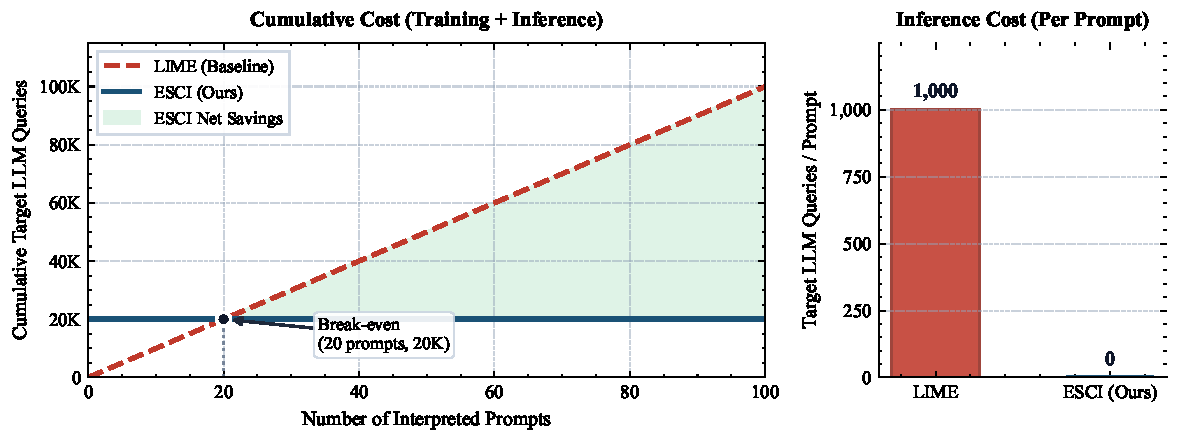
\includegraphics[width=\linewidth]{figures/Fig-INTERP-Computational-Scalability-V3.pdf}
    \caption{تحلیل مقیاس‌پذیری محاسباتی و هزینه‌ی استعلام}\label{fig:chap5_api_cost}
\end{figure}
\vspace{-0.25cm}

\paragraph{سرشکن‌سازی هزینه‌ها در \lr{ESCI}.}
در تقابل با روش‌های اختلالی، چارچوب \lr{ESCI} بخش عمده‌ی بار پردازشی را به فاز پیش‌آموزش شبکه‌ی جانشین منتقل می‌کند. پس از اتمام آموزش، استخراج انتساب برای هر ورودی جدید، نیازی به استعلام اضافی از مدل هدف نداشته و تنها با یک عبور پیش‌رو از شبکه‌ی مفسر در زمان پردازشی ثابت $\mathcal{O}(1)$ انجام می‌گیرد.

آموزش اولیه‌ی شبکه‌های انرژی و مفسر مستلزم هزینه‌ی اولیه‌ی استخراج داده است. با فرض اینکه تعداد نمونه‌های استعلام‌شده در فاز پیش‌آموزش برابر با $D_{\text{\lr{train}}} = 20000$ باشد، نقطه‌ی سربه‌سر محاسباتی میان \lr{ESCI} و خط‌پایه‌ی \lr{LIME} به‌صورت زیر محاسبه می‌گردد:
\begin{equation}
    N_{\text{\lr{break-even}}} = \frac{D_{\text{\lr{train}}}}{K_{\text{\lr{LIME\_Avg}}}} = \frac{20000}{1000} = 20
\end{equation}
این محاسبه نشان می‌دهد که هزینه‌ی اولیه‌ی آموزش چارچوب \lr{ESCI}، پس از ممیزی حدود ۲۰ پرامپت با طول متوسط در قیاس با \lr{LIME} مستهلک می‌گردد.

پویایی این مقیاس‌پذیری در شکل~\ref{fig:chap5_api_cost} نشان داده شده است. در نمودار میله‌ای سمت راست، تعداد استعلام‌های لازم در زمان استنتاج به ازای هر پرامپت مقایسه شده است که در \lr{ESCI} برابر با صفر است. در نمودار سمت چپ، روند هزینه‌ی تجمعی استعلام‌ها نشان می‌دهد که پس از نقطه‌ی سربه‌سر، هزینه‌ی حاشیه‌ای ممیزی در \lr{ESCI} ثابت می‌ماند.

\paragraph{محدودیت‌های ظرفیتی و چشم‌انداز آینده.}
در کنار مزیت محاسباتی، باید به محدودیت ظرفیت پارامتری مدل فعلی \lr{ESCI} نیز اشاره کرد. همان‌طور که در بخش‌های پیشین مشاهده شد، مفسر ۷۱ میلیون پارامتری ما در متون شدیداً ساختاریافته (نظیر \lr{WikiBio}) در تفکیک‌های ریزدانه‌ی کلید-مقدار عملکرد محتاطانه‌تری نسبت به اوراکل‌های چند میلیارد پارامتری نشان می‌دهد. فشرده‌سازی بازنمایی‌های پیچیده‌ی یک مدل زبانی بزرگ در یک جانشین نسبتاً سبک، با گلوگاه ظرفیتی همراه است. با این حال، نتایج تجربی این پژوهش اثبات می‌کند که با ارتقای مقیاس معماری مفسر و استفاده از داده‌های متنوع‌تر در آینده، می‌توان بدون از دست دادن مزیت استنتاج $\mathcal{O}(1)$، وضوح استخراج‌ها را بیش از پیش بهبود بخشید.

% !TEX root = ../thesis.tex
% ==============================================================================
%  CHAPTER 6: CONCLUSIONS & FUTURE WORK (فصل ششم: نتیجه‌گیری و کارهای آینده) (chapters/chapter6_conclusions.tex)
% ==============================================================================
%  This chapter summarizes the primary findings and contributions of the
%  thesis, addresses theoretical and computational limitations, and outlines
%  promising directions for future research.
% ==============================================================================

\chapter{نتیجه‌گیری و کارهای آتی}\label{chap:chapter6_conclusions}

این فصل به جمع‌بندی جامع مسیر طی‌شده در این پایان‌نامه، از صورت‌بندی صوری مسئله‌ی ممیزی مدل‌های زبانی بزرگ تا طراحی، پیاده‌سازی و ارزیابی تجربی چارچوب پیشنهادی اختصاص دارد. در ادامه، ابتدا دستاوردهای روش‌شناختی و تجربی پژوهش در پرتو نتایج حاصل از ارزیابی‌های تطبیقی در برابر خطوط پایه‌ی جعبه‌سفید و جعبه‌سیاه بازخوانی و صورت‌بندی می‌شوند. سپس، محدودیت‌های ساختاری، معرفت‌شناختی و محاسباتی حاکم بر مسئله‌ی انتساب در سیستم‌های مسدود واکاوی شده و در نهایت، افق‌های تحقیقاتی نوین برای گسترش و کاربست این رهیافت در بهینه‌سازی سامانه‌ها و ممیزی‌های کاربردی ترسیم می‌گردند.


\section{جمع‌بندی دستاوردها و نتایج}\label{sec:6-1}

هدف بنیادین این پژوهش، توسعه‌ی یک متدولوژی پساعملی و مستقل از مدل برای انتساب ویژگی در مدل‌های زبانی بزرگ با رژیم دسترسی جعبه‌سیاه بود؛ سناریویی که در آن تحلیل‌گر صرفاً به متن محقق‌شده‌ی ورودی و خروجی دسترسی دارد و پارامترها، گرادیان‌ها و حتی توزیع احتمالات خروجی (لوجیت‌ها) در پسِ رابط‌های تجاری مسدود شده‌اند. همان‌گونه که در مسئله‌ی~\ref{prob:chap1_causal_attribution} در فصل نخست و معادله‌ی~\ref{eq:chap4_constrained_opt} در فصل چهارم صورت‌بندی شد، چالش محوری در این بستر، یافتن بردار ماسک دودویی بهینه با نام $\mathbf{m}^* \in {\{0, 1\}}^N$ است که با اعمال بر روی $N$ جمله‌ی پرامپت ورودی ($\mathbf{x} = (x_1, \dots, x_N) \in \mathcal{S}^N$)، زیرمجموعه‌ی پیش‌آیندهای منتخب ($\mathbf{x}_S = \mathbf{x} \odot \mathbf{m}^*$) را برای تبیین زیرمجموعه‌ی هدف از جملات خروجی ($\mathbf{y}_T = {(y_j)}_{j \in T} \subseteq \mathbf{y}$) استخراج نماید:

\begin{equation}\label{eq:chap6_constrained_opt}
    \mathbf{m}^* = \arg\min_{\mathbf{m} \in {\{0, 1\}}^N} \|\mathbf{m}\|_0 \quad \text{به‌شرط آن‌که} \quad \mathcal{D}\big(f_\theta(\mathbf{x} \odot \mathbf{m}), \mathbf{y}_T\big) \le \epsilon
\end{equation}
که در آن $\|\cdot\|_0$ بیانگر اصل ضرورت و فشردگی، $\mathcal{D}$ سنجه‌ی واگرایی معنایی متناظر با اصل کفایت، و $\epsilon > 0$ آستانه‌ی خطای پذیرفتنی است. برای حل این مسئله‌ی بهینه‌سازی ترکیبیاتی بدون گرفتاری در پیچیدگی نمایی فضای حالات و بدون نیاز به استعلام‌های مکرر از مدل هدف، چارچوب جانشین مبتنی بر انرژی برای تفسیر در سطح مفهوم (\lr{ESCI}) طراحی، پیاده‌سازی و اعتبارسنجی شد. دستاوردهای این رویکرد را می‌توان در محورهای کلیدی زیر خلاصه نمود:

\paragraph{ارتقای واحد تحلیل به سطح گزاره و مهار خطای توزیعی.}
یکی از موانع ساختاری در روش‌های سنتی انتساب ویژگی در پردازش زبان طبیعی، تقلیل‌گرایی به سطح توکن‌های خرد است. دست‌کاری یا حذف توکن‌های منفرد در مدل‌های مولد خودهمبسته، گرامر متن را متلاشی کرده و منجر به بروز خطای داده‌های خارج از توزیع (\lr{OOD}) می‌شود؛ وضعیتی که در آن نوسان رفتار مدل صرفاً بازتابی از واکنش به تخریب ساختار نحوی است، نه نشانه‌ای از وابستگی محتوایی واقعی~\cite{madsen2022evaluating}. علاوه بر این، به دلیل پدیده‌ی افزونگی واژگانی، افت احتمال یک توکن خاص لزوماً به معنای محو بار معنایی آن مفهوم از خروجی نیست. در این پژوهش، با اتکا به مبانی فلسفی اصل بافتار فرگه~\cite{frege1991foundations} و نظریه‌ی شناختی ساخت‌وساز-ادغام کینتش~\cite{kintsch1998comprehension}، واحد تحلیل به سطح جمله به‌عنوان کوچک‌ترین حامل یک گزاره‌ی منطقی مستقل ارتقا یافت. این تغییر مقیاس بنیادین تضمین کرد که حذف یا گزینش مؤلفه‌های ورودی، هویت ساختاری و معنایی متن را حفظ کرده و پیش‌آیندهای استخراج‌شده به‌شکلی شفاف و انسان‌خوانا تبیین شوند.

\paragraph{مدل‌سازی چشم‌انداز انرژی جانشین بدون نیاز به نرمال‌سازی احتمالات.}
در شرایط انسداد رابط‌های تجاری، عدم‌دسترسی به بردار لوجیت‌ها مانع از به‌کارگیری معیارهای مشتق‌پذیر سنتی می‌شود، و از سوی دیگر، محاسبه‌ی تابع افراز بر روی فضای نامتناهی دنباله‌های متنی از نظر ریاضی غیرقابل‌حل است~\cite{lecun2006tutorial}. چارچوب \lr{ESCI} برای حل این معضل، یک مدل مبتنی بر انرژی (\lr{EBM}) با معماری ترنسفورمر دوسویه ($\mathcal{E}_{\text{\lr{LM}}}(\mathbf{x}, \mathbf{y}; \theta)$) را به‌عنوان ارزیاب انطباق‌پذیریِ نرمال‌نشده به‌کار می‌گیرد~\cite{bakhtin2019realfake, deng2020residual}. این شبکه با پرهیز از تولید متن (که خود منشأ بروز توهم تفسیرپذیری در مدل‌های خودتوضیح است)، تمام ظرفیت پارامتری خود را به ارزیابی یکپارچه‌ی ساختار پرامپت و پاسخ اختصاص می‌دهد. آموزش این مدل با بهره‌گیری از یک تابع زیان دوگانه مبتنی بر \lr{InfoNCE}~\cite{oord2018representation} شامل زیان وفاداری سراسری ($\mathcal{L}_{\text{\lr{fidelity}}}$) و زیان وابستگی محلی پادواقعی ($\mathcal{L}_{\text{\lr{dep}}}$) انجام می‌پذیرد. بدین‌ترتیب، مدل انرژی انطباق‌پذیری ساختاری و معنایی میان گزاره‌های ورودی و خروجی را بر مبنای متون مشاهده‌پذیر مدل هدف مدل‌سازی می‌کند، بدون آن‌که فرضی پیرامون یادگیری خمینه‌ها یا پویایی بازنمایی‌های درونی مدل جعبه‌سیاه اعمال شود.

\paragraph{استنتاج مستهلک‌شده و استخراج پیش‌آیندها در زمان‌ثابت $\mathcal{O}(1)$.}
روش‌های اختلالی کلاسیک نظیر \lr{LIME}~\cite{ribeiro2016lime} برای ارزیابی هر ورودی جدید، نیازمند کاوش در فضای ترکیبیاتی و ارسال صدها استعلام به رابط برنامه‌نویسی (\lr{API}) مدل هدف هستند که هزینه‌ی مالی و زمانی سنگینی را تحمیل می‌کند. در چارچوب \lr{ESCI}، با بهره‌گیری از پارادایم استنتاج مستهلک‌شده~\cite{tu2018learning, chen2018learning}، دانش توزیع‌شده در چشم‌انداز انرژی به یک شبکه‌ی مفسر مستقل ($\mathcal{IN}(\mathbf{x}, \mathbf{y}, T; \alpha)$) تقطیر می‌شود. مفسر با شرطی‌سازی بازنمایی‌ها بر روی شاخص‌های هدف خروجی ($T$) و مدل‌سازی انتخاب جملات به‌صورت توزیع‌های برنولی مستقل با استفاده از تابع سیگموئید، آموزش می‌بیند تا شکاف انرژی زیر را هم‌زمان با اعمال جریمه‌ی خلوتی نُرم $L_1$ بیشینه سازد:
\begin{equation}\label{eq:chap6_energy_gap}
    \Delta\mathcal{E}(\hat{\mathbf{m}}) = \mathcal{E}_{\text{\lr{LM}}}\big(\mathbf{x} \odot (\mathbf{1} - \hat{\mathbf{m}}), \mathbf{y}_T; \theta\big) - \mathcal{E}_{\text{\lr{LM}}}\big(\mathbf{x} \odot \hat{\mathbf{m}}, \mathbf{y}_T; \theta\big)
\end{equation}
این طراحی، بار محاسباتی را به فاز پیش‌آموزش منتقل کرده و در زمان استنتاج، پیش‌آیندهای اثرگذار را تنها با یک بار عبور پیش‌رو در گراف محاسباتی مفسر و در زمان‌ثابت $\mathcal{O}(1)$ بدون حتی یک استعلام از مدل هدف استخراج می‌نماید. تحلیل‌های تجربی نشان داد که نقطه‌ی سربه‌سر محاسباتی این رویکرد در مقایسه با روش‌های اختلالی پس از ممیزی تنها ۲۰ پرامپت با طول متوسط حاصل می‌شود و پس از آن، هزینه‌ی حاشیه‌ای ممیزی در \lr{ESCI} به صفر می‌رسد.

\paragraph{ارزیابی وفاداری تجربی در تقابل با خطوط پایه‌ی جعبه‌سفید و جعبه‌سیاه.}
برای سنجش جامع کیفیت انتساب، چارچوب پیشنهادی در دو مجموعه‌داده‌ی مکمل شامل \lr{HC3}~\cite{guo2023closechatgpthumanexperts} (پرسش و پاسخ آزاد مکالمه‌ای) و \lr{WikiBio}~\cite{lebret2016neural} (تولید متن مقید بر پایه‌ی داده‌های ساختاریافته) و بر روی سه مدل زبانی با معماری‌های ناهمگن شامل \lr{Llama–3.1–8B–Instruct}، \lr{Gemma–2–9B–It} و مدل تجاری مسدود \lr{GPT–4o–Mini} پیاده‌سازی و ارزیابی شد. ارزیابی وفاداری بر پایه‌ی یک خط‌لوله‌ی مداخله‌ای سه‌گانه شامل کفایت ($\mathcal{S}$)، جامعیت ($\mathcal{C}$) و شکاف وفاداری ($\Delta\mathcal{F} = \mathcal{S} - \mathcal{C}$) تحت سه عملگر محاسباتی متمایز انجام گرفت: استلزام منطقی صوری ($\mathcal{F}_{\text{\lr{NLI}}}$)، شباهت کسینوسی بیشینه‌ی جملات ($\mathcal{F}_{\text{\lr{cosine}}}$)، و لگاریتم احتمالات نرمال‌شده‌ی توکن‌ها ($\mathcal{F}_{\text{\lr{logprob}}}$)~\cite{carton2020evaluating, atanasova2023faithfulness}.

در این ارزیابی‌ها، عملکرد \lr{ESCI} هم در برابر طیف وسیعی از روش‌های جعبه‌سیاه (شامل هیئت اوراکل‌های زبانی، خودتوضیحی و درون‌نگری مدل‌های هدف، واریانت جعبه‌سیاه \lr{LIME} در سطح جمله، تطبیق رشته‌ای و خط‌پایه‌ی تصادفی خلوت دیریکله) و هم در تقابل با روش‌های دارای دسترسی ممتاز جعبه‌خاکستری و جعبه‌سفید (شامل توجه خام ترنسفورمر~\cite{vaswani2017attention}، بسط توجه~\cite{abnar2020quantifying}، گرادیان شاپ~\cite{lundberg2017unified}، ورودی ضرب‌در گرادیان~\cite{li2016visualizing, simonyan2014deepinside}، روش حذفی در سطح جمله یا \lr{Sentence-LOO}~\cite{li2017understanding, zeiler2014visualizing}، و واریانت جعبه‌خاکستری \lr{LIME}~\cite{ribeiro2016lime}) مورد سنجش قرار گرفت. 

نتایج تجربی نشان داد که اگرچه روش‌های جعبه‌سفید به دلیل دسترسی مستقیم به وزن‌ها، فعال‌سازی‌های پنهان و گرادیان‌ها از مزیتی ساختاری در سنجه‌های مبتنی بر افت احتمالات توکن‌ها برخوردارند، اما در سنجش وفاداری معنایی بر مبنای استلزام منطقی صوری ($\Delta\mathcal{F}_{\text{\lr{NLI}}}$)، مفسر جعبه‌سیاه \lr{ESCI} با ثبت شکاف‌های مثبت $0.108 \pm 0.004$ بر روی \lr{Llama–3.1} و $0.228 \pm 0.004$ بر روی \lr{Gemma–2}، عملکردی فراتر از مکانیزم‌های توجه درونی (شکاف $0.093$ و $0.084$) و ورودی ضرب‌در گرادیان (شکاف $-0.027$ و $+0.029$) به نمایش گذاشت و به روش‌های پرهزینه‌ی اختلالی نظیر \lr{Sentence-LOO} (شکاف $0.123$ و $0.295$) نزدیک شد. افزون بر این، در ارزیابی معقولیت انتساب بر روی \lr{WikiBio}، مفسر پیشنهادی هم‌راستایی رتبه‌ای بالایی با روش‌های جریان توجه (نمره‌ی \lr{nDCG} معادل $0.726$ با بسط توجه و $0.743$ با توجه خام) ثبت کرد که نشان می‌دهد چشم‌انداز انرژی سرشکن‌شده قادر است ساختار کلان وابستگی‌های گزاره‌ای را بدون نیاز به بازرسی لایه‌های درونی بازتاب دهد.

\paragraph{مرزبندی معرفت‌شناختی و سرنخ‌های عینی اثرگذاری.}
در نهایت، تأکید بر این نکته ضروری است که انتساب‌های استخراج‌شده در چارچوب \lr{ESCI} بر پایه‌ی الگوهای انطباق‌پذیری متنی در متون مشاهده‌پذیر شکل گرفته‌اند. به‌بیانی دیگر، پیش‌آیندهای شناسایی‌شده شواهد و نشانگرهایی تجربی و عینی از نحوه‌ی تأثیر اجزای پرامپت بر گزاره‌های خروجی فراهم می‌آورند که از نظر تجربی با خطوط زیربنایی تأثیرگذاری در مدل همسو هستند. نگریستن به مسئله‌ی انتساب جعبه‌سیاه از این زاویه، بستری عملی و محاسبه‌پذیر برای پژوهش‌های آتی در حوزه‌ی ممیزی مدل‌های مولد بنا می‌نهد.


\section{محدودیت‌های پژوهش}\label{sec:6-2}

علی‌رغم دستاوردهای روش‌شناختی و مزایای محاسباتی چارچوب \lr{ESCI}، استقرار و کاربست این متدولوژی با محدودیت‌های ساختاری و واقعیت‌های عینی حاکم بر محیط‌های جعبه‌سیاه روبه‌رو است که تبیین شفاف آن‌ها برای هدایت پژوهش‌های آینده الزامی است:

\paragraph{فقدان ذاتی حقیقت پایه و قلمرو رفتاری.}
ارزیابی وفاداری توضیحات در پردازش زبان طبیعی و مدل‌های مولد، به‌طور بنیادین با چالش فقدان حقیقت پایه‌ی قطعی و جهان‌شمول مواجه است~\cite{schneider2024explainable, moran2026towardinterpretable}. از آنجا که مسیرهای محاسباتی خودهمبسته در مدل‌های مسدود تجاری غیرقابل‌مشاهده و مات هستند، نه حاشیه‌نویسی‌های انسانی، نه نگاشت‌های مکاشفه‌ای مبتنی بر تطبیق واژگانی (نظیر معیارهای اعتبارسنجی خارجی \lr{AIS}~\cite{rashkin2023measuring} یا خط‌پایه‌ی تطبیق رشته‌ای)، و نه حتی سنجه‌های مداخله‌ای پادواقعی، هیچ‌یک استانداردی مطلق برای انتساب ارائه نمی‌دهند. این چالش، بازتاب‌دهنده‌ی یک محدودیت ساختاری در ماهیت ممیزی جعبه‌سیاه در پردازش زبان طبیعی است، و یک نقص الگوریتمی گذرا که با راهکارهای ساده برطرف شود نیست.

از یک سو، همان‌گونه که در ادبیات سنجه‌های تفسیرپذیری تبیین شده است، معیارهای مداخله‌ای می‌توانند تحت تأثیر قانون گودهارت دچار سوگیری ارزیابی شوند~\cite{ju2022logictraps, hsia2024goodhart}؛ وضعیتی که در آن مفسرها به‌جای انتساب گزاره‌های دارای نقش ساختاری، به‌سوی انتخاب بخش‌هایی سوق می‌یابند که بیشترین شوک توزیعی را در فضای خروجی ایجاد کنند. از سوی دیگر، یافته‌های تجربی این پژوهش در هم‌سویی با مطالعات کاماهی و یعقوب‌زاده~\cite{kamahi2024counterfactuals} نشان داد که مدل‌های زبانی در هنگام حذف جملات ورودی در آزمایش‌های جامعیت، به‌طور گسترده به دانش پارامتریک درونی خود تکیه می‌کنند؛ پدیده‌ای که مانع از سقوط کامل نمره‌ی جامعیت ($\mathcal{C}_{\text{\lr{omp}}}$) به صفر شده و مقادیر آن را در دامنه‌ی $0.42$ تا $0.60$ تثبیت می‌کند. در نتیجه‌ی این واقعیت‌های ساختاری، چارچوب \lr{ESCI} یک سازوکار انتساب رفتاری بر پایه‌ی الگوهای همبستگی ساختاری ورودی-خروجی ارائه می‌دهد و نباید آن را با بازرسی مدارهای مکانیکی در لایه‌های پنهان شبکه هم‌ارز دانست~\cite{elhage2021mathematical, friedman2023comparing}. بر این اساس، به‌جای جستجوی یک حقیقت پایه‌ی دست‌نیافتنی، گسترش ارزیابی‌ها در بسترهای عملیاتی متنوع‌تر برای سنجش پایداری انتساب تحت شرایط گوناگون دنیای واقعی ضروری خواهد بود.

\paragraph{سربار محاسباتی پیش‌آموزش در برابر استنتاج مستهلک‌شده.}
اگرچه چارچوب \lr{ESCI} با دستیابی به پیچیدگی زمان‌ثابت $\mathcal{O}(1)$ نیاز به استعلام‌های مکرر در زمان استنتاج را به صفر می‌رساند، اما این کارایی عملیاتی از طریق انتقال بار پردازشی به فاز پیش‌آموزش حاصل می‌شود. تولید دادگان جفت‌های پرامپت-پاسخ ($20,000$ نمونه و حتی بیشتر)، ساخت نمونه‌های منفی تقابلی، و اجرای فرایند لنگراندازی دوره‌ای برای همگام نگه‌داشتن مدل انرژی با مفسر، مستلزم صرف هزینه و زمان اولیه در تعامل با \lr{API} مدل هدف است. اگرچه این هزینه پس از ممیزی تعداد محدودی پرامپت (نقطه‌ی سربه‌سر در مقایسه با \lr{LIME}) کاملاً مستهلک می‌شود، اما برای کاربردهایی که با وظایف گذرا و تک‌نمونه‌ای سروکار دارند یا کاربرانی با محدودیت‌های پردازشی شدید، پرداخت این هزینه‌ی اولیه‌ی آماده‌سازی نیازمند برنامه‌ریزی منابع است.

\paragraph{تخصیص وظیفه‌محور و محدودیت ظرفیت مدل‌های جانشین فشرده.}
به‌منظور امکان‌پذیر ساختن آموزش و استقرار چارچوب بر روی سخت‌افزارهای متعارف و در دسترس (نظیر دو پردازنده‌ی گرافیکی \lr{NVIDIA T4})، مدل‌های جانشین انرژی و مفسر در این پژوهش با ساختاری سبک و ظرفیت پارامتری فشرده (مجموعاً ۱۸۱ میلیون پارامتر که تنها حدود ۷۱ میلیون آن در مفسر آموزش‌پذیر است) پیکربندی شدند. این طراحی متمرکز، اگرچه عملکرد مناسبی در یادگیری الگوهای هم‌نشینی در دامنه‌های آزمون (مانند مکالمات روزمره‌ی \lr{HC3} و بیوگرافی‌های \lr{WikiBio}) به‌همراه دارد، اما بازنمایی‌های آموخته‌شده را وابسته به دامنه‌ی داده‌های آموزشی می‌سازد. مطابق با مشاهدات بختیین و همکاران~\cite{bakhtin2019realfake} پیرامون افت دقت مدل‌های انرژی در تعمیم بین‌دامنه‌ای در غیاب داده‌های ترکیبی، مفسری که منحصراً بر روی متون عمومی آموزش دیده است، بدون گذراندن فاز پیش‌آموزش تکمیلی یا ارتقای ظرفیت پارامتری، قابلیت تعمیم مستقیم به متون تخصصی (نظیر اسناد حقوقی پیچیده یا متون پزشکی تخصصی) را نخواهد داشت.

\paragraph{کران‌های تفکیک‌پذیری در سطح جمله.}
انتخاب جمله به‌عنوان مفهوم اتمیک و واحد عملیاتی تحلیل، اگرچه از فروپاشی نحوی و افتادن در دام شوک‌های توزیعی ناشی از اختلالات توکن‌محور جلوگیری می‌کند، اما به‌طور ساختاری حد بالایی برای تفکیک‌پذیری معنایی تعیین می‌نماید. در متون زبانی پیچیده، یک جمله‌ی مرکب و طولانی ممکن است شامل چندین گزاره‌ی فرعی، قیود شرطی و اطلاعات توصیفی متمایز باشد. در ساختار فعلی، مفسر کل جمله را به‌صورت یک گزاره‌ی یکپارچه ارزیابی می‌کند که این امر تفکیک دقیق‌تر سهم هر یک از عبارات درون‌جمله‌ای را ناممکن می‌سازد.


\section{پیشنهادها برای تحقیقات آتی}\label{sec:6-3}

بر پایه‌ی دستاوردهای به‌دست‌آمده، اعتبارسنجی‌های تجربی و محدودیت‌های شناسایی‌شده، مسیرهای پژوهشی زیر برای گسترش و تکامل این متدولوژی پیشنهاد می‌گردد:

\paragraph{مقیاس‌پذیری در پیکره‌های چندوظیفه‌ای و بافتارهای طولانی.}
گام نخست در جهت ارتقای تعمیم‌پذیری چارچوب \lr{ESCI}، افزایش مقیاس پارامتری شبکه‌های جانشین و آموزش آن‌ها بر روی پیکره‌های چندوظیفه‌ای و متون چنددامنه‌ای گسترده است تا مفسر بتواند قابلیت تعمیم‌پذیری بدون نیاز به تنظیم مجدد را در مواجهه با پرامپت‌های ناآشنا به‌دست آورد. علاوه بر این، در رویارویی با اسناد بسیار طولانی در سیستم‌های تولید تقویت‌شده با بازیابی (\lr{RAG})، بازطراحی ماژول‌های توجه متقاطع با استفاده از مکانیزم‌های توجه سلسله‌مراتبی، امکان ارزیابی دوگانه در دو سطح کلان (پاراگراف‌ها و بخش‌ها) و خرد (جملات) را فراهم خواهد ساخت تا مقیاس‌پذیری محاسباتی برای پنجره‌های بافتار وسیع تضمین گردد.

\paragraph{فشرده‌سازی خودکار پرامپت.}
فراتر از کاربردهای ممیزی و تفسیرپذیری، توانایی استخراج سریع پیش‌آیندهای اثرگذار، ظرفیت بالایی برای بهینه‌سازی مستقیم سامانه‌های زبانی ارائه می‌دهد. ماسک‌های خلوت تولیدشده توسط شبکه‌ی مفسر می‌توانند به‌عنوان مبنایی برای فشرده‌سازی خودکار پرامپت پیش از ارسال به مدل‌های تجاری به‌کار روند. با حذف پیشینی جملات فاقد ارزش انتسابی از بافتار، طول پرامپت ارسالی به رابط‌های برنامه‌نویسی کاهش می‌یابد که این امر مستقیماً به کاهش تأخیر استنتاج و افت چشمگیر هزینه‌های مالی در سیستم‌های بلادرنگ منجر خواهد شد.

\paragraph{ممیزی و اعتبارسنجی استدلال در زنجیره‌ی افکار.}
در استدلال‌های گام‌به‌گام و چندمرحله‌ای مدل‌های زبانی نظیر پرامپت‌گذاری زنجیره‌ی افکار~\cite{wei2022chain}، مدل‌ها مستعد افتادن در دام استدلال هدفمند، توجیهات نادرست و توهمات متنی هستند~\cite{turpin2023language}. چشم‌انداز انرژی چارچوب \lr{ESCI} می‌تواند به‌عنوان یک ناظر و ارزیاب مستقل بر زنجیره‌ی استدلال عمل کند. در این الگو، با ارزیابی انطباق‌پذیری انرژی میان هر گام میانی با گزاره‌های ماقبل خود، مراحلی که دارای عدم‌انطباق بالایی در چشم‌انداز انرژی هستند شناسایی شده و به‌عنوان خطاهای استدلالی پیش از تولید پاسخ نهایی فیلتر یا تصحیح می‌گردند.

\paragraph{توسعه به مدل‌های بینایی-زبانی و دامنه‌ی چندوجهی.}
اصول ساختاری حاکم بر چارچوب \lr{ESCI} به زبان متنی محدود نبوده و قابل‌تعمیم به مدل‌های چندوجهی است. با جایگزینی واحد جمله با بخش‌های ساختاریافته‌ی تصویر یا اجزای قطعه‌بندی‌شده‌ی معنایی در مدل‌های بینایی-زبانی، می‌توان یک چشم‌انداز انرژی مشترک میان نواحی بصری و گزاره‌های متنی آموزش داد.

\paragraph{ارزیابی‌های تعاملی و سنجش اثرگذاری بر کاربر انسان.}
پیرو مبانی نظری دوشی-ولز و کیم~\cite{doshivelez2017rigorous} مبنی بر لزوم ارزیابی‌های کاربردمحور در تفسیرپذیری، گام ضروری بعدی، اجرای مطالعات بالینی با حضور کاربران انسانی در حلقه‌ی سیستم (حوزه‌ی تعامل انسان و رایانه) است. سنجش این امر که آیا ارائه‌ی پیش‌آیندهای گزاره‌ایِ استخراج‌شده توسط \lr{ESCI} در عمل سرعت، دقت و اعتماد کالیبره‌شده‌ی تحلیل‌گران را در فرایندهای ممیزی، تصحیح خطاها و اعتبارسنجی اسناد افزایش می‌دهد یا خیر، معیاری تعیین‌کننده برای میزان اثربخشی این متدولوژی در محیط‌های عملیاتی دنیای واقعی خواهد بود.

\vspace{0.5cm}
در پایان، این پایان‌نامه با پایه‌ریزی چارچوب \lr{ESCI}، گامی در جهت عبور از رویکردهای تقلیل‌گرای توکن‌محور به‌سوی تفسیرپذیری محاسباتی و معنادار در سطح مفاهیم برداشت. با تلفیق مدل‌سازی انرژی در سطح گزاره‌ها و تقطیر دانش در یک مفسر مستهلک‌شده، این پژوهش نشان داد که می‌توان رفتار مدل‌های زبانی عظیم و مسدود را بدون نقض محدودیت‌های دسترسی جعبه‌سیاه، با مقداری خطا در زمان‌ثابتِ استنتاج ممیزی کرد. امید است که پایه‌های نظری و تجربی استوارشده در این رساله، افق‌های نوینی را برای شفافیت ساختاری و استقرار مسئولانه‌ی نسل‌های آینده‌ی هوش مصنوعی مولد بگشاید.


% ==============================================================================
% 5. BIBLIOGRAPHY & GLOSSARIES (مراجع و واژه‌نامه‌ها)
% ==============================================================================
% Academic bibliography with hyperlinked DOI/URLs
% !TEX root = ../thesis.tex
% ==============================================================================
%  BIBLIOGRAPHY CONFIGURATION & LOADER (bibliography/bibliography.tex)
% ==============================================================================
%
%  This file sets up the bibliography layout, citation environment, and data sources.
%
% ------------------------------------------------------------------------------
%  HOW IT WORKS:
% ------------------------------------------------------------------------------
%  - BibTeX Style: Uses `bibliography/unsrtabbrv.bst`, an enhanced unsrt style
%    modernized to turn paper titles into clickable hyperlinks when `doi` or `url`
%    fields are present, and display other fields selectively based on standards. 
%  - Data Sources: Points to `bibliography/refs.bib` (main citations) and
%    `bibliography/full.bib` (extended/secondary references).
%  - Uncited references: Uncomment `\nocite{*}` if you wish to display all entries
%    in the `.bib` files regardless of whether they were cited with `\cite{...}`.
%  - Spacing: Configured with compact, professional inter-item spacing.
% ==============================================================================

\clearpage
{\phantomsection}
\addcontentsline{toc}{chapter}{مراجع}

\begin{latin}
\small
\linespread{1.15}\selectfont
\setlength{\parskip}{0pt}

% Compact, elegant academic bibliography spacing
\let\oldthebibliography\thebibliography{}
\let\endoldthebibliography\endthebibliography{}
\renewenvironment{thebibliography}[1]{%
  \begin{oldthebibliography}{#1}%
    \small
    \linespread{1.15}\selectfont
    \setlength{\parskip}{0pt}%
    \setlength{\parsep}{0pt}%
    \setlength{\itemsep}{0.25em plus 0.05em minus 0.05em}%
}{%
  \end{oldthebibliography}%
}

\bibliographystyle{bibliography/unsrtabbrv}

% Uncomment next line to include uncited references in the output:
% \nocite{*}

\bibliography{bibliography/refs,bibliography/full}
 
\end{latin}


% Dependency tracking for LaTeX Workshop & compiler dependency graphs
\setbox0=\vbox{% !TEX root = ../thesis.tex
% ==============================================================================
%  BIDIRECTIONAL THESIS GLOSSARY & DICTIONARY REPOSITORY (backmatter/words.tex)
% ==============================================================================
%
%  WELCOME TO THE THESIS GLOSSARY FILE!
%  This file is the SINGLE SOURCE OF TRUTH for all technical terms and
%  translations used in the thesis.
%
% ------------------------------------------------------------------------------
%  HOW TO ADD NEW TERMS (دستورالعمل افزودن واژگان):
% ------------------------------------------------------------------------------
%  Simply add term pairs anywhere in this file using the following syntax:
%
%      \dictentry{English Term}{معادل فارسی}
%
%  Examples:
%      \dictentry{neural network}{شبکه‌ی عصبی}
%      \dictentry{attention mechanism}{مکانیزم توجه}
%      \dictentry{loss function}{تابع زیان}
%
% ------------------------------------------------------------------------------
%  COMPILATION & AUTOMATIC SORTING PIPELINE:
% ------------------------------------------------------------------------------
%  1. You do NOT need to sort entries manually! Add them in any order.
%  2. When compiling via `latexmk` or VS Code LaTeX Workshop:
%     The build hook in `latexmkrc` automatically executes:
%         python scripts/build_dictionaries.py
%  3. If compiling manually via `xelatex`:
%     Run `python scripts/build_dictionaries.py` in your terminal whenever
%     you add or modify terms in this file.
%  4. The python script automatically:
%     - Generates `backmatter/dict_fa2en_content.tex` sorted by Persian alphabet.
%     - Generates `backmatter/dict_en2fa_content.tex` sorted by English alphabet.
%     - Handles special Persian characters (پ، چ، ژ، گ، آ) and ignores
%       zero-width non-joiners (\u200c / نیم‌فاصله) for strictly correct collation.
%     - Groups entries by letter headers (\dicalphabet{...}).
%  5. DO NOT EDIT `dict_fa2en_content.tex` or `dict_en2fa_content.tex` directly,
%     as they are automatically overwritten by the build script.
% ==============================================================================

% \dictentry{English Term}{Persian Translation}
%  Automatic sorting & grouping is performed upon compilation.
% -------------------------------------------------------


\dictentry{ablation}{حذف}
\dictentry{accuracy}{دقت}
\dictentry{activation}{فعال‌سازی}
\dictentry{activation function}{تابع فعال‌سازی}
\dictentry{activation patching}{وصله‌زنی فعال‌سازی}
\dictentry{AdamW}{بهینه‌ساز ادام‌دبلیو}
\dictentry{additive update}{به‌روزرسانی افزایشی}
\dictentry{adversarial}{متخاصم}
\dictentry{adversarial attack}{حمله‌ی متخاصم}
\dictentry{adversarial attacks}{حملات متخاصم}
\dictentry{affine transformation}{تبدیل آفین}
\dictentry{AIS}{انتساب‌پذیر به منابع مشخص}
\dictentry{aligned}{هم‌تراز}
\dictentry{aligned at the start}{هم‌تراز در مبدأ}
\dictentry{alignment}{هم‌ترازی}
\dictentry{allocation}{تخصیص}
\dictentry{alternating local-global attention}{توجه متناوب محلی و سراسری}
\dictentry{amortized}{سرشکن}
\dictentry{amortized inference}{استنتاج مستهلک‌شده}
\dictentry{annotation artifacts}{آرتیفکت‌های حاشیه‌نویسی}
\dictentry{antecedent}{پیش‌آیند}
\dictentry{antecedents}{پیش‌آیندها}
\dictentry{AOPC}{سطح روی منحنی اختلال}
\dictentry{API}{رابط برنامه‌نویسی}
\dictentry{application}{کاربرد}
\dictentry{application-grounded evaluation}{ارزیابی کاربردمحور}
\dictentry{application programming interface}{رابط برنامه‌نویسی}
\dictentry{approximation}{تقریب}
\dictentry{architecture}{معماری}
\dictentry{argument}{آرگومان}
\dictentry{artifact impact ratio}{نسبت تأثیر آرتیفکت}
\dictentry{artificial intelligence}{هوش مصنوعی}
\dictentry{artificial neural network}{شبکه‌ی عصبی مصنوعی}
\dictentry{attention}{توجه}
\dictentry{attention flow}{جریان توجه}
\dictentry{attention masking}{ماسک‌گذاری توجه}
\dictentry{attention mechanism}{مکانیزم توجه}
\dictentry{attention pooling}{تجمیع مبتنی بر توجه}
\dictentry{attention rollout}{بسط توجه}
\dictentry{attention score}{امتیاز توجه}
\dictentry{attention weights}{وزن‌های توجه}
\dictentry{Attributable to Identified Sources}{انتساب‌پذیر به منابع مشخص}
\dictentry{attribution}{انتساب}
\dictentry{attribution patching}{وصله‌زنی انتسابی}
\dictentry{augmented views}{دیدگاه‌های افزوده}
\dictentry{autoencoder}{خودرمزگذار}
\dictentry{automated prompt optimization}{بهینه‌سازی خودکار پرامپت}
\dictentry{autoregressive}{خودهمبسته}
\dictentry{autoregressive attention}{توجه خودهمبسته}
\dictentry{autoregressive model}{مدل خودهمبسته}
\dictentry{autoregressive structured prediction}{پیش‌بینی ساختاریافته‌ی خودهمبسته}
\dictentry{backpropagation}{پس‌انتشار}
\dictentry{backward pass}{پس‌رو}
\dictentry{baseline}{خط‌پایه}
\dictentry{batch}{دسته}
\dictentry{batch size}{اندازه‌ی دسته}
\dictentry{beam search}{جستجوی پرتو}
\dictentry{benchmark}{محک}
\dictentry{benchmark dataset}{مجموعه‌داده‌ی محک}
\dictentry{Bernoulli distribution}{توزیع برنولی}
\dictentry{BERTScore}{معیار برت‌اسکور}
\dictentry{bias}{سوگیری}
\dictentry{bidirectional}{دوسویه}
\dictentry{bidirectional self-attention}{خودتوجهی دوسویه}
\dictentry{binary}{دودویی}
\dictentry{binary hypercube}{ابرمکعب دودویی}
\dictentry{binary mask vector}{بردار ماسک دودویی}
\dictentry{black-box}{جعبه‌سیاه}
\dictentry{black-box model}{مدل جعبه‌سیاه}
\dictentry{BLEU}{معیار بلو}
\dictentry{block-diagonal}{بلوک-قطری}
\dictentry{Boolean lattice}{مشبکه‌ی بولی}
\dictentry{bottleneck}{گلوگاه}
\dictentry{broadcasting}{پخش‌پذیری}
\dictentry{budget constraint}{قید بودجه}
\dictentry{byte-pair encoding}{رمزگذاری جفت‌بایت}
\dictentry{candidate}{کاندیدا}
\dictentry{capacity}{ظرفیت}
\dictentry{cardinality}{کاردینالیتی}
\dictentry{causal}{علّی}
\dictentry{causal abstraction}{انتزاع علّی}
\dictentry{causal attention}{توجه علّی}
\dictentry{causal inner product}{ضرب داخلی علّی}
\dictentry{causality loss}{زیان علّیت}
\dictentry{causal mask}{ماسک علّی}
\dictentry{causal representation learning}{یادگیری بازنمایی علّی}
\dictentry{causal tracing}{ردیابی علّی}
\dictentry{center point}{نقطه‌ی مرکزی}
\dictentry{chain-of-thought}{زنجیره‌ی افکار}
\dictentry{chain-of-verification}{زنجیره‌ی اعتبارسنجی}
\dictentry{chain rule of probability}{قاعده‌ی ضرب احتمالات}
\dictentry{checkpoint}{نقطه‌ی بازرسی}
\dictentry{circuit}{مدار}
\dictentry{circuit discovery}{کشف مدار}
\dictentry{classification}{دسته‌بندی}
\dictentry{classification head}{سر دسته‌بندی}
\dictentry{classifier}{دسته‌بند}
\dictentry{classify}{دسته‌بندی کردن}
\dictentry{clique}{کلیک}
\dictentry{closed commercial systems}{سیستم‌های تجاری و بسته}
\dictentry{coherence-intervention trade-off}{مصالحه‌ی انسجام-مداخله}
\dictentry{combinatorial optimization}{بهینه‌سازی ترکیبیاتی}
\dictentry{combinatorial space}{فضای ترکیبیاتی}
\dictentry{compact}{فشرده}
\dictentry{compactness}{فشردگی}
\dictentry{compatibility}{انطباق‌پذیری}
\dictentry{compatibility function}{تابع انطباق‌پذیری}
\dictentry{compatibility pattern}{الگوی انطباق‌پذیری}
\dictentry{compatibility patterns}{الگوهای انطباق‌پذیری}
\dictentry{completeness}{کامل‌بودن}
\dictentry{complexity}{پیچیدگی}
\dictentry{component attribution}{انتساب مؤلفه}
\dictentry{compositional concept extraction}{استخراج مفهوم ترکیب‌پذیر}
\dictentry{comprehensiveness}{جامعیت}
\dictentry{compression}{فشرده‌سازی}
\dictentry{computational complexity}{پیچیدگی محاسباتی}
\dictentry{computational cost}{هزینه‌ی محاسباتی}
\dictentry{computational efficiency}{کارایی محاسباتی}
\dictentry{computational graph}{گراف محاسباتی}
\dictentry{concatenation}{الحاق}
\dictentry{concept}{مفهوم}
\dictentry{concept activation vector}{بردار فعال‌سازی مفهوم}
\dictentry{concept-based explanation}{توضیح مبتنی بر مفهوم}
\dictentry{concept bottleneck}{گلوگاه مفهومی}
\dictentry{concept bottleneck model}{مدل گلوگاه مفهومی}
\dictentry{concept bottleneck models}{مدل‌های گلوگاه مفهومی}
\dictentry{concept embedding model}{مدل تعبیه‌ی مفهوم}
\dictentry{concept-level}{در سطح مفهوم}
\dictentry{concept representation}{بازنمایی مفهوم}
\dictentry{conceptual explainer}{مفسر مفهومی}
\dictentry{Concrete distribution}{توزیع کانکریت}
\dictentry{conditional masked language model}{مدل زبانی ماسک‌شده‌ی شرطی}
\dictentry{conditional noise contrastive estimation}{تخمین تقابلی نویز شرطی}
\dictentry{conditional probability distribution}{توزیع احتمال شرطی}
\dictentry{conditional random field}{میدان تصادفی شرطی}
\dictentry{consistency}{سازگاری}
\dictentry{constant-time}{زمان‌ثابت}
\dictentry{constrained combinatorial optimization}{بهینه‌سازی ترکیبیاتی مقید}
\dictentry{constrained text generation}{تولید متن مقید}
\dictentry{construction-integration}{ساخت‌وساز-ادغام}
\dictentry{Construction-Integration model}{مدل ساخت‌وساز-ادغام}
\dictentry{context}{بافتار}
\dictentry{context length}{طول بافتار}
\dictentry{context-length probing}{کاوش طول بافتار}
\dictentry{context principle}{اصل بافتار}
\dictentry{contextual embedding}{تعبیه‌ی بافتاری}
\dictentry{contextualized embedding}{تعبیه‌ی بافتاری}
\dictentry{context window}{پنجره‌ی بافتار}
\dictentry{continuous}{پیوسته}
\dictentry{continuous relaxation}{آزادسازی پیوسته}
\dictentry{contrastive}{تقابلی}
\dictentry{contrastive divergence}{واگرایی تقابلی}
\dictentry{contrastive feature attribution}{انتساب ویژگی تقابلی}
\dictentry{contrastive learning}{یادگیری تقابلی}
\dictentry{contrastive loss}{زیان تقابلی}
\dictentry{contrastive training}{آموزش تقابلی}
\dictentry{convergence}{همگرایی}
\dictentry{convex}{محدب}
\dictentry{convolution}{پیچش}
\dictentry{convolutional}{پیچشی}
\dictentry{convolutional network}{شبکه‌ی پیچشی}
\dictentry{cooperative game theory}{نظریه‌ی بازی‌های همکارانه}
\dictentry{corpus}{پیکره}
\dictentry{cosine similarity}{شباهت کسینوسی}
\dictentry{cost-augmented}{افزوده-با-هزینه}
\dictentry{cost function}{تابع هزینه}
\dictentry{counterfactual}{پادواقعی}
\dictentry{counterfactual explanations}{توضیحات پادواقعی}
\dictentry{counterfactual pair}{جفت پادواقعی}
\dictentry{counterfactual sampling}{نمونه‌برداری پادواقعی}
\dictentry{cover}{پوشش}
\dictentry{credit attribution}{انتساب اعتبار}
\dictentry{critic}{منتقد}
\dictentry{cross-attention}{توجه متقاطع}
\dictentry{cross-attention layer}{لایه‌ی توجه متقاطع}
\dictentry{cross-encoder}{رمزگذار متقاطع}
\dictentry{cross-entropy}{آنتروپی متقاطع}
\dictentry{cross-entropy loss}{زیان آنتروپی متقاطع}
\dictentry{cross-validation}{اعتبارسنجی متقاطع}
\dictentry{data}{داده}
\dictentry{data augmentation}{افزایش داده}
\dictentry{data mining}{داده‌کاوی}
\dictentry{dataset}{مجموعه‌داده}
\dictentry{data-to-text generation}{تولید متن از روی داده}
\dictentry{debugging}{عیب‌یابی}
\dictentry{decision boundary}{مرز تصمیم}
\dictentry{decision function}{تابع تصمیم}
\dictentry{decision tree}{درخت تصمیم}
\dictentry{decoder}{رمزگشا}
\dictentry{decoding}{رمزگشایی}
\dictentry{decoding strategy}{راهبرد رمزگشایی}
\dictentry{deep learning}{یادگیری عمیق}
\dictentry{deep Taylor decomposition}{تجزیه‌ی تیلور عمیق}
\dictentry{deep value networks}{شبکه‌های ارزش عمیق}
\dictentry{degree}{درجه}
\dictentry{deletion AUC}{سطح زیر منحنی حذف}
\dictentry{denoising k-sparse autoencoder}{خودرمزگذار نویزگیر کا-خلوت}
\dictentry{dense}{متراکم}
\dictentry{density}{تراکم}
\dictentry{dependency parsing}{تجزیه‌ی وابستگی}
\dictentry{deterministic}{قطعی}
\dictentry{dictionary learning}{یادگیری دیکشنری}
\dictentry{differentiation operator}{عملگر مشتق‌پذیری}
\dictentry{differentiation operators}{عملگرهای مشتق‌پذیری}
\dictentry{diffusion model}{مدل انتشاری}
\dictentry{dimension}{بُعد}
\dictentry{dimensionality reduction}{کاهش ابعاد}
\dictentry{direct preference optimization}{بهینه‌سازی مستقیم ترجیحات}
\dictentry{discrete}{گسسته}
\dictentry{discrete diffusion}{مدل انتشاری گسسته}
\dictentry{discrete tokens}{توکن‌های گسسته}
\dictentry{discriminative}{متمایزگر}
\dictentry{discriminator}{متمایزگر}
\dictentry{disentangled representation}{بازنمایی تفکیک‌شده}
\dictentry{disentangled representations}{بازنمایی‌های تفکیک‌شده}
\dictentry{distance}{فاصله}
\dictentry{distributed}{توزیع‌شده}
\dictentry{distributed alignment search}{جستجوی هم‌ترازی توزیع‌شده}
\dictentry{distributed representation}{بازنمایی توزیع‌شده}
\dictentry{distribution}{توزیع}
\dictentry{distributional hypothesis}{فرضیه‌ی توزیعی}
\dictentry{distributional shift}{شوک توزیعی}
\dictentry{divergence}{واگرایی}
\dictentry{dominate}{غلبه}
\dictentry{dot product}{ضرب نقطه‌ای}
\dictentry{doubling}{دوبرابرسازی}
\dictentry{downstream task}{وظیفه‌ی پایین‌دست}
\dictentry{DPO}{بهینه‌سازی مستقیم ترجیحات}
\dictentry{dropout}{رهاسازی}
\dictentry{Dyck languages}{زبان‌های دایک}
\dictentry{edge}{یال}
\dictentry{efficiency}{کارایی}
\dictentry{efficient}{کارا}
\dictentry{eigenvector}{بردار ویژه}
\dictentry{element-wise product}{ضرب درایه‌به‌درایه}
\dictentry{embedding}{تعبیه}
\dictentry{embedding space}{فضای تعبیه}
\dictentry{empirical faithfulness}{وفاداری تجربی}
\dictentry{encoder}{رمزگذار}
\dictentry{encoder-decoder}{رمزگذار-رمزگشا}
\dictentry{end-to-end}{انتها‌به‌انتها}
\dictentry{energy-based model}{مدل مبتنی بر انرژی}
\dictentry{energy-based reranking}{رتبه‌بندی مجدد مبتنی بر انرژی}
\dictentry{energy-based reward model}{مدل پاداش مبتنی بر انرژی}
\dictentry{energy-based surrogate}{جانشین مبتنی بر انرژی}
\dictentry{energy gap}{شکاف انرژی}
\dictentry{energy landscape}{چشم‌انداز انرژی}
\dictentry{energy network}{شبکه‌ی انرژی}
\dictentry{energy separation margin}{حاشیه‌ی تفکیک انرژی}
\dictentry{entanglement}{درهم‌تنیدگی}
\dictentry{entropy}{آنتروپی}
\dictentry{epoch}{ایپاک}
\dictentry{ERASER}{محک ایریسر}
\dictentry{erasure metric}{معیار فرسایشی}
\dictentry{erasure metrics}{معیارهای فرسایشی}
\dictentry{ESCI}{جانشین مبتنی بر انرژی برای تفسیر در سطح مفهوم}
\dictentry{estimation}{برآورد}
\dictentry{Euclidean distance}{فاصله‌ی اقلیدسی}
\dictentry{evaluation}{ارزیابی}
\dictentry{evaluation metric}{معیار ارزیابی}
\dictentry{evidence lower bound}{کران پایین شواهد}
\dictentry{expectation}{امید ریاضی}
\dictentry{experimental}{تجربی}
\dictentry{explainability}{توضیح‌پذیری}
\dictentry{explainable AI}{هوش مصنوعی توضیح‌پذیر}
\dictentry{exponential}{نمایی}
\dictentry{exponential decay}{افت نمایی}
\dictentry{exponential kernel}{هسته‌ی نمایی}
\dictentry{exposure bias}{سوگیری مواجهه}
\dictentry{extreme}{حدی}
\dictentry{faithfulness}{وفاداری}
\dictentry{faithfulness evaluation}{ارزیابی وفاداری}
\dictentry{feature}{ویژگی}
\dictentry{feature attribution}{انتساب ویژگی}
\dictentry{feature extraction}{استخراج ویژگی}
\dictentry{feature importance}{اهمیت ویژگی}
\dictentry{feature map}{نقشه‌ی ویژگی}
\dictentry{feature omission}{حذف ویژگی}
\dictentry{feature selection}{انتخاب ویژگی}
\dictentry{feedforward}{پیش‌خور}
\dictentry{feedforward layer}{لایه‌ی پیش‌خور}
\dictentry{feedforward neural network}{شبکه‌ی عصبی پیش‌خور}
\dictentry{feedforward sublayer}{زیرلایه‌ی پیش‌خور}
\dictentry{few-shot prompting}{پرامپت‌دهی چندنمونه‌ای}
\dictentry{fidelity}{وفاداری}
\dictentry{fine-tuning}{تنظیم ظریف}
\dictentry{finite alphabet}{الفبای متناهی}
\dictentry{flatten}{تخت کردن}
\dictentry{flattening}{مسطح کردن}
\dictentry{foil}{پادنمونه}
\dictentry{foil class}{کلاس پادنمونه}
\dictentry{formal}{رسمی}
\dictentry{forward pass}{پیش‌رو}
\dictentry{free energy}{انرژی آزاد}
\dictentry{freeze}{انجماد}
\dictentry{frontier}{مرزی}
\dictentry{frozen}{منجمد}
\dictentry{frozen model}{مدل منجمد}
\dictentry{functionally-grounded evaluation}{ارزیابی کارکردمحور}
\dictentry{fuzzy string matching}{تطبیق فازی رشته‌ها}
\dictentry{generalization}{تعمیم‌پذیری}
\dictentry{generalization bound}{کران تعمیم}
\dictentry{generalization error}{خطای تعمیم}
\dictentry{generation}{تولید}
\dictentry{generative}{مولد}
\dictentry{generative adversarial network}{شبکه‌ی مولد تخاصمی}
\dictentry{generative AI auditing}{ممیزی هوش مصنوعی مولد}
\dictentry{generative explainable AI}{هوش مصنوعی مولد تفسیرپذیر}
\dictentry{generative model}{مدل مولد}
\dictentry{generator-evaluator gap}{فرضیه‌ی شکاف تولیدکننده-ارزیاب}
\dictentry{geometric instability}{ناپایداری هندسی}
\dictentry{geometric stability}{پایداری هندسی}
\dictentry{Gibbs-Boltzmann distribution}{توزیع گیبس-بولتزمن}
\dictentry{Gibbs sampling}{نمونه‌برداری گیبس}
\dictentry{glass-box}{جعبه‌شیشه‌ای}
\dictentry{global average pooling}{تجمیع میانگین سراسری}
\dictentry{global minimum}{کمینه سراسری}
\dictentry{global negative}{نمونه‌ی منفی سراسری}
\dictentry{Goodhart's law}{قانون گودهارت}
\dictentry{GPU hours}{ساعت محاسباتی کارت گرافیک}
\dictentry{gradient}{گرادیان}
\dictentry{gradient ascent}{گرادیان افزایشی}
\dictentry{gradient descent}{گرادیان کاهشی}
\dictentry{gradient saturation}{اشباع گرادیان}
\dictentry{graph}{گراف}
\dictentry{gray-box}{جعبه‌خاکستری}
\dictentry{gray-box model}{مدل جعبه‌خاکستری}
\dictentry{greedy}{حریصانه}
\dictentry{greedy coordinate gradient}{گرادیان مختصات حریصانه}
\dictentry{greedy decoding}{رمزگشایی حریصانه}
\dictentry{greedy matching}{تطبیق حریصانه}
\dictentry{grounding}{لنگراندازی}
\dictentry{ground-truth}{حقیقت پایه}
\dictentry{grouped-query attention}{توجه پرسمان گروهی}
\dictentry{Gumbel-max trick}{ترفند گامبل-مکس}
\dictentry{Gumbel-softmax}{گامبل-سافت‌مکس}
\dictentry{Hadamard product}{ضرب هادامارد}
\dictentry{half-space}{نیم‌فضا}
\dictentry{hallucination}{توهم}
\dictentry{hallucination mitigation}{کاهش توهم}
\dictentry{Hamming distance}{فاصله‌ی همینگ}
\dictentry{hard negative sample}{نمونه‌ی منفی سخت}
\dictentry{hardware specification}{مشخصات سخت‌افزاری}
\dictentry{HC3}{پیکره‌ی مقایسه‌ای انسان و چت‌جی‌پی‌تی}
\dictentry{heuristic}{اکتشافی}
\dictentry{hidden bias}{سوگیری پنهان}
\dictentry{hidden biases}{سوگیری‌های پنهان}
\dictentry{hidden layer}{لایه‌ی پنهان}
\dictentry{hidden state}{حالت پنهان}
\dictentry{hierarchical}{سلسله‌مراتبی}
\dictentry{high dimensions}{ابعاد بالا}
\dictentry{high-impact concepts}{مفاهیم پرنفوذ}
\dictentry{high-stakes domain}{حوزه‌ی پرمخاطره}
\dictentry{high-stakes domains}{حوزه‌های پرمخاطره}
\dictentry{hinge loss}{زیان مفصلی}
\dictentry{human-computer interaction}{تعامل انسان و رایانه}
\dictentry{human-grounded evaluation}{ارزیابی انسان‌محور}
\dictentry{hyperparameter}{ابرپارامتر}
\dictentry{hypothesis space}{فضای فرضیه}
\dictentry{identifiability}{همانندپذیری}
\dictentry{importance mask}{ماسک اهمیت}
\dictentry{importance sampling}{نمونه‌برداری اهمیتی}
\dictentry{in-batch negative}{نمونه‌ی منفی درون‌دسته}
\dictentry{in-context learning}{یادگیری درون‌بافتاری}
\dictentry{induction}{استقرا}
\dictentry{induction head}{سر استقرایی}
\dictentry{inductive bias}{سوگیری استقرایی}
\dictentry{inference}{استنتاج}
\dictentry{inference time}{زمان استنتاج}
\dictentry{influence function}{تابع نفوذ}
\dictentry{influence functions}{توابع نفوذ}
\dictentry{InfoNCE}{تخمین تقابلی نویز اطلاعاتی}
\dictentry{information bottleneck}{گلوگاه اطلاعاتی}
\dictentry{information gain}{افزایش اطلاعات}
\dictentry{information leakage}{نشت اطلاعات}
\dictentry{information retrieval}{بازیابی اطلاعات}
\dictentry{initialization}{مقداردهی اولیه}
\dictentry{inpainter}{شبکه‌ی ترمیم‌کننده}
\dictentry{input layer}{لایه‌ی ورودی}
\dictentry{input reduction}{کاهش ورودی}
\dictentry{insertion AUC}{سطح زیر منحنی درج}
\dictentry{instance}{نمونه}
\dictentry{instance-wise feature selection}{انتخاب ویژگی در سطح نمونه}
\dictentry{instruction-tuning}{تنظیم مبتنی بر دستورالعمل}
\dictentry{integrated gradients}{گرادیان‌های یکپارچه}
\dictentry{interactive}{تعاملی}
\dictentry{intermediate activations}{فعال‌سازی‌های میانی}
\dictentry{interpretability}{تفسیرپذیری}
\dictentry{interpreter}{مفسر}
\dictentry{intervention}{مداخله}
\dictentry{intractable}{غیرقابل‌حل}
\dictentry{intrinsic}{درونی}
\dictentry{invariant}{ناوردا}
\dictentry{inverse Hessian matrix}{معکوس ماتریس هسین}
\dictentry{inversion}{نابه‌جایی}
\dictentry{iteration}{تکرار}
\dictentry{iterative refinement}{پالایش تکرارشونده}
\dictentry{Jacobian matrix}{ماتریس ژاکوبی}
\dictentry{joint energy model}{مدل انرژی مشترک}
\dictentry{kernel}{هسته}
\dictentry{key}{کلید}
\dictentry{K-FAC}{تقریب انحنای فاکتورگیری‌شده‌ی کرونکر}
\dictentry{Kleene closure}{بستار کلینی}
\dictentry{knowledge base}{پایگاه دانش}
\dictentry{knowledge distillation}{تقطیر دانش}
\dictentry{Kronecker product}{ضرب کرونکر}
\dictentry{Kullback-Leibler divergence}{واگرایی کولبک-لایبلر}
\dictentry{L2X}{یادگیری برای توضیح}
\dictentry{label-free concept bottleneck model}{مدل گلوگاه مفهومی بدون‌برچسب}
\dictentry{label noise}{نویز برچسب}
\dictentry{Lagrange multipliers}{ضرب‌کننده‌های لاگرانژ}
\dictentry{Langevin dynamics}{دینامیک لانژون}
\dictentry{language model}{مدل زبانی}
\dictentry{large concept model}{مدل مفهومی بزرگ}
\dictentry{large language model}{مدل زبانی بزرگ}
\dictentry{large language models}{مدل‌های زبانی بزرگ}
\dictentry{LASSO}{لاسو}
\dictentry{LASSO Regression}{رگرسیون لاسو}
\dictentry{latency}{تأخیر}
\dictentry{latent debate}{مناظره پنهان}
\dictentry{latent space}{فضای پنهان}
\dictentry{latent variable}{متغیر پنهان}
\dictentry{layer}{لایه}
\dictentry{layer normalization}{نرمال‌سازی لایه‌ای}
\dictentry{layer-wise relevance propagation}{انتشار لایه‌به‌لایه‌ی ارتباط}
\dictentry{learnable}{قابل‌یادگیری}
\dictentry{learnable positional embeddings}{تعبیه‌های موقعیتی قابل‌یادگیری}
\dictentry{learning from AI feedback}{یادگیری از بازخورد هوش مصنوعی}
\dictentry{learning rate}{نرخ یادگیری}
\dictentry{learning rate warmup}{گرم‌کردن نرخ یادگیری}
\dictentry{learning to explain}{یادگیری برای توضیح}
\dictentry{leave-one-out}{حذف یکی}
\dictentry{lexical overlap}{هم‌پوشانی واژگانی}
\dictentry{lexical redundancy}{افزونگی واژگانی}
\dictentry{likelihood}{درست‌نمایی}
\dictentry{LIME}{توضیحات محلی تفسیرپذیر مستقل از مدل}
\dictentry{linear}{خطی}
\dictentry{linear combination}{ترکیب خطی}
\dictentry{linear probe}{کاوشگر خطی}
\dictentry{linear probes}{کاوشگرهای خطی}
\dictentry{linear programming}{برنامه‌ریزی خطی}
\dictentry{linear regression}{رگرسیون خطی}
\dictentry{linear representation hypothesis}{فرضیه‌ی بازنمایی خطی}
\dictentry{linear separability}{تفکیک‌پذیری خطی}
\dictentry{Lipschitz continuous}{پیوسته لیپشیتس}
\dictentry{local accuracy}{دقت محلی}
\dictentry{local interpreter}{مفسر محلی}
\dictentry{local minimum}{کمینه محلی}
\dictentry{local negative}{نمونه‌ی منفی محلی}
\dictentry{local optimum}{بهینه‌ی محلی}
\dictentry{logit}{لوجیت}
\dictentry{logit lens}{لنز لوجیت}
\dictentry{logits}{لوجیت‌ها}
\dictentry{logit soft-capping}{کنترل نرم لوجیت‌ها}
\dictentry{log-odds}{نسبت لگاریتم شانس}
\dictentry{loss}{زیان}
\dictentry{loss function}{تابع زیان}
\dictentry{loss landscape}{چشم‌انداز زیان}
\dictentry{machine learning}{یادگیری ماشین}
\dictentry{manifold}{خمینه}
\dictentry{margin}{حاشیه}
\dictentry{marginal contribution}{مشارکت حاشیه‌ای}
\dictentry{marginal distribution}{توزیع حاشیه‌ای}
\dictentry{margin-based}{حاشیه‌محور}
\dictentry{margin loss}{زیان حاشیه‌ای}
\dictentry{Markov chain}{زنجیره‌ی مارکوف}
\dictentry{Markov chain Monte Carlo}{مونت‌کارلوی زنجیره‌ی مارکوف}
\dictentry{Markov random field}{میدان تصادفی مارکوف}
\dictentry{masked language model}{مدل زبانی ماسک‌شده}
\dictentry{masking}{ماسک‌گذاری}
\dictentry{matrix}{ماتریس}
\dictentry{matrix multiplication}{ضرب ماتریسی}
\dictentry{max-flow}{بیشینه-جریان}
\dictentry{maximum}{بیشینه}
\dictentry{maximum likelihood}{بیشینه‌ی درست‌نمایی}
\dictentry{max pooling}{تجمیع بیشینه}
\dictentry{MCMC}{مونت‌کارلوی زنجیره‌ی مارکوف}
\dictentry{mean absolute error}{میانگین قدرمطلق خطا}
\dictentry{mean-field inference}{استنتاج میدان میانگین}
\dictentry{mean pooling}{تجمیع میانگین}
\dictentry{mean squared error}{میانگین مربعات خطا}
\dictentry{mechanistic}{مکانیکی}
\dictentry{mechanistic interpretability}{تفسیرپذیری مکانیکی}
\dictentry{memory footprint}{ردپای حافظه}
\dictentry{metacognitive prompting}{پرامپت‌دهی فراشناختی}
\dictentry{mini-batch}{ریزدسته}
\dictentry{minimum}{کمینه}
\dictentry{mixture of experts}{ترکیب خبرگان}
\dictentry{mixture of softmaxes}{ترکیب سافت‌مکس‌ها}
\dictentry{modality}{وجه}
\dictentry{model-agnostic}{مستقل از مدل}
\dictentry{model capacity}{ظرفیت مدل}
\dictentry{model editing}{ویرایش مدل}
\dictentry{monosemantic}{تک‌معنایی}
\dictentry{monosemanticity}{تک‌معنایی}
\dictentry{Monte Carlo}{مونت‌کارلو}
\dictentry{motivated reasoning}{استدلال هدفمند}
\dictentry{multi-concept prompt learning}{یادگیری پرامپت چندمفهومی}
\dictentry{multi-head attention}{توجه چندسره}
\dictentry{multimodal}{چندوجهی}
\dictentry{multitask learning}{یادگیری چندوظیفه‌ای}
\dictentry{mutual information}{اطلاعات متقابل}
\dictentry{natural language}{زبان طبیعی}
\dictentry{natural language explanation}{تبیین مبتنی بر زبان طبیعی}
\dictentry{natural language inference}{استنتاج زبان طبیعی}
\dictentry{natural language processing}{پردازش زبان طبیعی}
\dictentry{necessity}{ضرورت}
\dictentry{negative log-likelihood}{منفی لگاریتم درست‌نمایی}
\dictentry{negative pair}{جفت منفی}
\dictentry{negative sampling}{نمونه‌برداری منفی}
\dictentry{neighborhood}{همسایگی}
\dictentry{neural architecture}{معماری عصبی}
\dictentry{neural network}{شبکه‌ی عصبی}
\dictentry{next sentence prediction}{پیش‌بینی جمله‌ی بعدی}
\dictentry{n-gram}{ان-گرم}
\dictentry{node}{گره}
\dictentry{noise-contrastive estimation}{تخمین تقابلی نویز}
\dictentry{non-autoregressive}{غیرخودهمبسته}
\dictentry{non-autoregressive translation}{ترجمه‌ی غیرخودهمبسته}
\dictentry{non-differentiability}{مشتق‌ناپذیری}
\dictentry{non-linearity}{غیرخطی‌بودن}
\dictentry{non-negative matrix factorization}{تجزیه‌ی ماتریس نامنفی}
\dictentry{nonparametric}{غیرپارامتری}
\dictentry{norm}{نرم}
\dictentry{normalization}{نرمال‌سازی}
\dictentry{normalized discounted cumulative gain}{بهره‌ی تجمعی تنزیل‌یافته‌ی نرمال‌شده}
\dictentry{NP-complete}{مسئله‌ی ان‌پی کامل}
\dictentry{NP-hard}{مسئله‌ی ان‌پی سخت}
\dictentry{nucleus sampling}{نمونه‌برداری هسته‌ای}
\dictentry{numerical underflow}{زیرسیلان عددی}
\dictentry{object}{شیء}
\dictentry{objective function}{تابع هدف}
\dictentry{observational interpretability}{تفسیرپذیری مشاهده‌ای}
\dictentry{Occam's razor}{تیغ اوکام}
\dictentry{occlusion}{انسداد}
\dictentry{one-hot vector}{بردار یک‌گانه}
\dictentry{online}{برخط}
\dictentry{opacity}{عدم‌شفافیت}
\dictentry{open-domain}{دامنه‌ی باز}
\dictentry{optimal ablation}{حذف بهینه}
\dictentry{optimization}{بهینه‌سازی}
\dictentry{optimum}{بهینه}
\dictentry{oracle}{اوراکل}
\dictentry{orthogonal}{متعامد}
\dictentry{outlier}{پرت}
\dictentry{outlier data}{داده‌ی پرت}
\dictentry{out-of-distribution}{خارج از توزیع}
\dictentry{out-of-vocabulary}{خارج از دایره‌ی واژگان}
\dictentry{output layer}{لایه‌ی خروجی}
\dictentry{output probability vector}{بردار احتمالات خروجی}
\dictentry{overcomplete}{فراتکمیل}
\dictentry{overfitting}{بیش‌برازش}
\dictentry{padding}{پدینگ}
\dictentry{padding mask}{ماسک پدینگ}
\dictentry{pairwise ranking accuracy}{دقت رتبه‌بندی زوجی}
\dictentry{parallelization}{موازی‌سازی}
\dictentry{parameter}{پارامتر}
\dictentry{parameter space}{فضای پارامترها}
\dictentry{parametric}{پارامتری}
\dictentry{parser}{تجزیه‌گر}
\dictentry{partition}{تقسیم‌بندی}
\dictentry{partition function}{تابع افراز}
\dictentry{parts-based representation}{بازنمایی مبتنی بر اجزا}
\dictentry{performance-interpretability trade-off}{مصالحه‌ی عملکرد-شفافیت}
\dictentry{periodic grounding}{لنگراندازی دوره‌ای}
\dictentry{permutation equivariant}{هم‌وردا با جایگشت}
\dictentry{perplexity}{حیرت}
\dictentry{perturbation}{اختلال}
\dictentry{perturbation-based}{مبتنی بر اختلال}
\dictentry{perturbation curve}{منحنی اختلال}
\dictentry{phatic expressions}{عبارات فاتیک}
\dictentry{pipeline}{خط‌لوله}
\dictentry{placeholder}{جای‌نگه‌دار}
\dictentry{planar}{مسطح}
\dictentry{plausibility}{معقولیت}
\dictentry{plausibility evaluation}{ارزیابی معقولیت}
\dictentry{pointwise}{نقطه‌به‌نقطه}
\dictentry{polysemanticity}{چندمعنایی}
\dictentry{pooling}{تجمیع}
\dictentry{pooling layer}{لایه‌ی تجمیع}
\dictentry{positional embedding}{تعبیه‌ی موقعیتی}
\dictentry{positional encoding}{رمزگذاری موقعیتی}
\dictentry{position-wise feedforward}{پیش‌خور موقعیت‌محور}
\dictentry{position-wise feed-forward network}{شبکه‌ی پیش‌خور موقعیت‌محور}
\dictentry{positive pair}{جفت مثبت}
\dictentry{post-hoc}{پساعملی}
\dictentry{post-hoc concept bottleneck model}{مدل گلوگاه مفهومی پساعملی}
\dictentry{precision}{دقت}
\dictentry{prediction}{پیش‌بینی}
\dictentry{pre-processing}{پیش‌پردازش}
\dictentry{pre-trained}{پیش‌آموزش‌دیده}
\dictentry{pre-training}{پیش‌آموزش}
\dictentry{privileged access}{دسترسی ممتاز}
\dictentry{probability density function}{تابع چگالی احتمال}
\dictentry{probability distribution}{توزیع احتمال}
\dictentry{projection}{تصویرسازی}
\dictentry{projection head}{سر تصویرسازی}
\dictentry{prompt}{پرامپت}
\dictentry{prompt engineering}{مهندسی پرامپت}
\dictentry{prompt injection}{تزریق پرامپت}
\dictentry{prompt-response}{پرامپت-پاسخ}
\dictentry{prompts contrastive loss}{زیان تقابلی پرامپت‌ها}
\dictentry{prompt trigger}{محرک پرامپت}
\dictentry{prompt-tuning}{تنظیم پرامپت}
\dictentry{propagating activation differences}{انتشار تفاوت فعال‌سازی‌ها}
\dictentry{propositional}{گزاره‌ای}
\dictentry{proposition space}{فضای گزاره‌ها}
\dictentry{pruning}{هرس}
\dictentry{pseudo-norm}{شبه‌نرم}
\dictentry{punctuation}{علائم نگارشی}
\dictentry{qualitative analysis}{تحلیل کیفی}
\dictentry{quantitative analysis}{تحلیل کمّی}
\dictentry{query}{پرسمان}
\dictentry{RAG}{تولید تقویت‌شده با بازیابی}
\dictentry{random variable}{متغیر تصادفی}
\dictentry{random walk}{گشت تصادفی}
\dictentry{rank}{رتبه}
\dictentry{rank deficiency}{کمبود رتبه}
\dictentry{rank-one model editing}{ویرایش مدل رتبه‌یک}
\dictentry{rationalization}{دلیل‌تراشی}
\dictentry{reasoning}{استدلال}
\dictentry{recall}{بازخوانی}
\dictentry{reconstruction}{بازسازی}
\dictentry{reconstruction loss}{زیان بازسازی}
\dictentry{recurrent neural network}{شبکه‌ی عصبی بازگشتی}
\dictentry{regex}{عبارت منظم}
\dictentry{regression}{رگرسیون}
\dictentry{regular expression}{عبارت منظم}
\dictentry{regularization}{منظم‌سازی}
\dictentry{regularization term}{جمله‌ی منظم‌سازی}
\dictentry{regularizer}{منظم‌ساز}
\dictentry{reinforcement learning}{یادگیری تقویتی}
\dictentry{reinforcement learning from AI feedback}{یادگیری تقویتی با بازخورد هوش مصنوعی}
\dictentry{reinforcement learning from human feedback}{یادگیری تقویتی با بازخورد انسانی}
\dictentry{remove and retrain}{حذف و آموزش مجدد}
\dictentry{reparameterization trick}{ترفند بازپارامتربندی}
\dictentry{representation}{بازنمایی}
\dictentry{representation collapse}{فروپاشی بازنمایی}
\dictentry{reranking}{رتبه‌بندی مجدد}
\dictentry{residual}{باقیمانده}
\dictentry{residual connection}{اتصال باقیمانده}
\dictentry{residual energy-based model}{مدل انرژی پسماند}
\dictentry{residual stream}{جریان باقیمانده}
\dictentry{response}{پاسخ}
\dictentry{response sequence}{توالی پاسخ}
\dictentry{retrieval-augmented generation}{تولید تقویت‌شده با بازیابی}
\dictentry{reward}{پاداش}
\dictentry{reward hacking}{تقلب در پاداش}
\dictentry{RLAIF}{یادگیری تقویتی با بازخورد هوش مصنوعی}
\dictentry{RLHF}{یادگیری تقویتی با بازخورد انسانی}
\dictentry{robustness}{استحکام}
\dictentry{ROUGE}{معیار روژ}
\dictentry{rule-based system}{سامانه‌ی مبتنی بر قاعده}
\dictentry{runtime}{زمان اجرا}
\dictentry{saddle point}{نقطه‌ی زینی}
\dictentry{safety auditing}{ممیزی ایمنی}
\dictentry{salience}{برجستگی}
\dictentry{saliency map}{نقشه‌ی برجستگی}
\dictentry{sampler}{نمونه‌بردار}
\dictentry{sample size}{اندازه‌ی نمونه}
\dictentry{sampling}{نمونه‌برداری}
\dictentry{satisfiability}{صدق‌پذیری}
\dictentry{scalability}{مقیاس‌پذیری}
\dictentry{scalar}{اسکالر}
\dictentry{scaled dot-product attention}{توجه نقطه‌ای مقیاس‌یافته}
\dictentry{score matching}{تطبیق امتیاز}
\dictentry{search space}{فضای جستجو}
\dictentry{segmentation}{تقطیع}
\dictentry{self-attention}{خودتوجهی}
\dictentry{self-attention attribution}{انتساب خودتوجهی}
\dictentry{self-attention layer}{لایه‌ی خودتوجهی}
\dictentry{self-consistency}{سازگاری درونی}
\dictentry{SelfIE}{خودتفسیری تعبیه‌ها}
\dictentry{self-normalizing}{خودنرمال‌ساز}
\dictentry{self-normalizing importance sampling}{نمونه‌برداری اهمیتی خودنرمال‌ساز}
\dictentry{self-supervised learning}{یادگیری خود‌نظارتی}
\dictentry{semantic}{معنایی}
\dictentry{semantic gap}{شکاف معنایی}
\dictentry{semantic pseudo-distance}{شبه‌فاصله‌ی معنایی}
\dictentry{semantic segmentation}{تقطیع معنایی}
\dictentry{semantic segmentation network}{شبکه‌ی تقطیع معنایی}
\dictentry{semantic textual similarity}{شباهت معنایی متون}
\dictentry{semantic-visual priors}{پیش‌فرض‌های بصری-معنایی}
\dictentry{semi-nonnegative matrix factorization}{فاکتورگیری ماتریس نیمه‌نامنفی}
\dictentry{semi-supervised learning}{یادگیری نیمه‌بانظارت}
\dictentry{sentence}{جمله}
\dictentry{sentence-level}{در سطح جمله}
\dictentry{sentence pooling}{تجمیع جملات}
\dictentry{sentence segmentation}{تقطیع جمله}
\dictentry{separable}{جداپذیر}
\dictentry{sequence}{توالی}
\dictentry{sequence-to-sequence}{توالی‌به‌توالی}
\dictentry{set}{مجموعه}
\dictentry{SHAP}{توضیحات افزایشی شاپلی}
\dictentry{Shapley additive explanations}{توضیحات افزایشی شاپلی}
\dictentry{Shapley value}{مقدار شاپلی}
\dictentry{Siamese network}{شبکه‌ی سیامی}
\dictentry{sigmoid}{سیگموئید}
\dictentry{similarity metric}{معیار شباهت}
\dictentry{simplex}{سیمپلکس}
\dictentry{single-selection collapse}{فروپاشی تک‌انتخابی}
\dictentry{Sobol indices}{شاخص‌های سوبول}
\dictentry{softmax}{سافت‌مکس}
\dictentry{SOInter}{مفسر خروجی ساختاریافته}
\dictentry{source attribution}{انتساب به منبع}
\dictentry{space}{فضا}
\dictentry{sparse}{خلوت}
\dictentry{sparse autoencoder}{خودرمزگذار خلوت}
\dictentry{sparse autoencoders}{خودرمزگذارهای خلوت}
\dictentry{sparse mixture of experts}{ترکیب خلوت خبرگان}
\dictentry{sparse representation}{بازنمایی خلوت}
\dictentry{sparsifier}{خلوت‌ساز}
\dictentry{sparsity}{خلوتی}
\dictentry{sparsity-constrained}{مقید به خلوتی}
\dictentry{spatial localization}{محلی‌سازی فضایی}
\dictentry{spatial mask}{ماسک مکانی}
\dictentry{Spearman's rank correlation}{همبستگی رتبه‌ای اسپیرمن}
\dictentry{spoofing}{جعل}
\dictentry{stability}{پایداری}
\dictentry{static embeddings}{تعبیه‌های ایستا}
\dictentry{steering vector}{بردار هدایت‌گر}
\dictentry{step-unrolling}{باز کردن گام‌به‌گام}
\dictentry{stochastic}{تصادفی}
\dictentry{stopword}{ایست‌واژه}
\dictentry{stopwords}{ایست‌واژه‌ها}
\dictentry{structural constraint}{محدودیت ساختاری}
\dictentry{structure-aware loss function}{تابع زیان آگاه به ساختار}
\dictentry{structured masking}{ماسک‌گذاری ساختاریافته}
\dictentry{structured prediction}{پیش‌بینی ساختاریافته}
\dictentry{sublinear}{زیرخطی}
\dictentry{subspace}{زیرفضا}
\dictentry{subword}{زیرواژه}
\dictentry{subword tokenization}{توکن‌سازی زیرواژه‌ای}
\dictentry{sufficiency}{کفایت}
\dictentry{superposition}{برهم‌نهی}
\dictentry{supervised learning}{یادگیری با‌نظارت}
\dictentry{surrogate}{جانشین}
\dictentry{surrogate interpreter}{مفسر جانشین}
\dictentry{surrogate model}{مدل جانشین}
\dictentry{symmetric Dirichlet distribution}{توزیع دیریکله‌ی متقارن}
\dictentry{syntactic collapse}{فروپاشی نحوی}
\dictentry{syntactic segmentation operator}{عملگر تقطیع نحوی}
\dictentry{syntactic structure}{ساختار نحوی}
\dictentry{target model}{مدل هدف}
\dictentry{target subset}{زیرمجموعه‌ی هدف}
\dictentry{temperature}{دما}
\dictentry{temperature annealing}{تبرید دما}
\dictentry{tensor}{تانسور}
\dictentry{test set}{مجموعه‌ی آزمون}
\dictentry{test-time intervention}{مداخله در زمان آزمون}
\dictentry{textbase}{پایگاه متن}
\dictentry{text generation}{تولید متن}
\dictentry{textual entailment}{استلزام متنی}
\dictentry{threshold}{آستانه}
\dictentry{time complexity}{پیچیدگی زمانی}
\dictentry{token}{توکن}
\dictentry{token embedding}{تعبیه‌ی توکن}
\dictentry{tokenization}{توکن‌سازی}
\dictentry{tokenize}{توکن‌سازی کردن}
\dictentry{tokenizer}{توکن‌ساز}
\dictentry{top-k sampling}{نمونه‌برداری تاپ-کی}
\dictentry{top-p sampling}{نمونه‌برداری تاپ-پی}
\dictentry{total variation distance}{فاصله‌ی تغییرات کل}
\dictentry{tracing}{ردیابی}
\dictentry{trade-off}{مصالحه}
\dictentry{training data}{داده آموزشی}
\dictentry{training dynamics}{دینامیک آموزش}
\dictentry{training set}{مجموعه‌ی آموزشی}
\dictentry{transfer learning}{یادگیری انتقالی}
\dictentry{transformation}{تبدیل}
\dictentry{transformer}{ترنسفورمر}
\dictentry{transition}{انتقال}
\dictentry{transition probability}{احتمال انتقال}
\dictentry{transparent}{شفاف}
\dictentry{tree-of-thoughts}{درخت افکار}
\dictentry{triplet loss}{زیان سه‌گانه}
\dictentry{truncate}{برش زدن}
\dictentry{truncated randomized search}{جستجوی تصادفی بریده‌شده}
\dictentry{truncation}{کوتاه‌سازی}
\dictentry{tuned lens}{لنز تنظیم‌شده}
\dictentry{tuning}{تنظیم}
\dictentry{two-dimensional}{جفت‌بُعد}
\dictentry{uncertainty}{عدم‌قطعیت}
\dictentry{underfitting}{کم‌برازش}
\dictentry{unembedding}{تعبیه‌زدایی}
\dictentry{unembedding matrix}{ماتریس تعبیه‌زدایی}
\dictentry{unembedding space}{فضای تعبیه‌زدایی}
\dictentry{uniform distribution}{توزیع یکنواخت}
\dictentry{unit of analysis}{واحد تحلیل}
\dictentry{unit vector}{بردار یکه}
\dictentry{unnormalized}{نرمال‌نشده}
\dictentry{unnormalized compatibility function}{تابع انطباق‌پذیری نرمال‌نشده}
\dictentry{unroll}{باز کردن محاسباتی}
\dictentry{unsupervised learning}{یادگیری بی‌نظارت}
\dictentry{validation set}{مجموعه‌ی اعتبارسنجی}
\dictentry{value}{ارزش}
\dictentry{variance}{واریانس}
\dictentry{variational autoencoder}{خودرمزگذار متغیر}
\dictentry{variational Bayesian}{بیزی متغیر}
\dictentry{variational lower bound}{کران پایین متغیر}
\dictentry{vector}{بردار}
\dictentry{vector space}{فضای برداری}
\dictentry{vertex}{رأس}
\dictentry{Vision Transformer}{ترنسفورمر بینایی}
\dictentry{vocabulary}{دایره‌ی واژگان}
\dictentry{warmup steps}{گام‌های گرم‌کردن}
\dictentry{weight decay}{کاهش وزن}
\dictentry{weight matrix}{ماتریس وزن‌ها}
\dictentry{white-box}{جعبه‌سفید}
\dictentry{white-box model}{مدل جعبه‌سفید}
\dictentry{zero-shot}{صفر-نمونه}
\dictentry{zero-shot chain-of-thought}{استدلال زنجیره‌ای صفر-نمونه}
\dictentry{zero-shot CoT}{استدلال زنجیره‌ای صفر-نمونه}
\dictentry{zeroth-order query model}{مدل پرس‌وجوی مرتبه‌صفر}
\dictentry{absolute position}{موقعیت مطلق}
\dictentry{analytic philosophy of language}{فلسفه‌ی تحلیلی زبان}
\dictentry{angular frequency}{بسامد زاویه‌ای}
\dictentry{application-grounded}{کاربردمحور}
\dictentry{attention weights matrix}{ماتریس وزن‌های توجه}
\dictentry{attractive force}{نیروی جاذبه}
\dictentry{base transformer}{ترنسفورمر پایه}
\dictentry{batch normalization}{نرمال‌سازی دسته‌ای}
\dictentry{BERT}{مدل برت}
\dictentry{bias vector}{بردار سوگیری}
\dictentry{binary classification}{دسته‌بندی دودویی}
\dictentry{binary importance mask}{ماسک اهمیت دودویی}
\dictentry{black-box regime}{رژیم جعبه‌سیاه}
\dictentry{BPE}{رمزگذاری جفت‌بایت}
\dictentry{causal self-attention}{خودتوجهی علّی}
\dictentry{cliques}{کلیک‌ها}
\dictentry{cognitive psychology}{روان‌شناسی شناختی}
\dictentry{community theory}{نظریه‌ی جوامع}
\dictentry{complexity penalty}{جریمه‌ی پیچیدگی}
\dictentry{complete graph}{گراف کامل}
\dictentry{conditional mutual information}{اطلاعات متقابل شرطی}
\dictentry{conditional random fields}{میدان‌های تصادفی شرطی}
\dictentry{CRF}{میدان تصادفی شرطی}
\dictentry{DeepNN}{شبکه‌ی عصبی عمیق}
\dictentry{distributed representations}{بازنمایی‌های توزیع‌شده}
\dictentry{dynamic programming}{برنامه‌ریزی پویا}
\dictentry{EBM}{مدل مبتنی بر انرژی}
\dictentry{end-of-sequence token}{توکن پایان توالی}
\dictentry{energy-based models}{مدل‌های مبتنی بر انرژی}
\dictentry{Euclidean norm}{نرم اقلیدسی}
\dictentry{feedforward network}{شبکه‌ی پیش‌خور}
\dictentry{feedforward networks}{شبکه‌های پیش‌خور}
\dictentry{FFN}{شبکه‌ی پیش‌خور}
\dictentry{finite sequence}{دنباله‌ی متناهی}
\dictentry{finite sequences}{دنباله‌های متناهی}
\dictentry{forward-backward algorithm}{الگوریتم پیشرو-پسرو}
\dictentry{fuzzy graph}{گراف فازی}
\dictentry{geometric progression}{تصاعد هندسی}
\dictentry{global feature selection}{انتخاب ویژگی سراسری}
\dictentry{GPT}{مدل جی‌پی‌تی}
\dictentry{Gumbel noise}{نویز گامبل}
\dictentry{hard negative samples}{نمونه‌های منفی سخت}
\dictentry{high-stakes}{پرمخاطره}
\dictentry{information noise-contrastive estimation}{تخمین تقابلی نویز اطلاعاتی}
\dictentry{INVASE}{روش اینویس}
\dictentry{joint distribution}{توزیع توأم}
\dictentry{key matrix}{ماتریس کلیدها}
\dictentry{KL divergence}{واگرایی کولبک-لایبلر}
\dictentry{L0 pseudo-norm}{شبه‌نرم صفر}
\dictentry{LayerNorm}{نرمال‌سازی لایه‌ای}
\dictentry{linear algebra}{جبر خطی}
\dictentry{LLaMA}{مدل لاما}
\dictentry{LLM}{مدل زبانی بزرگ}
\dictentry{LN}{نرمال‌سازی لایه‌ای}
\dictentry{local potential}{پتانسیل محلی}
\dictentry{local potentials}{پتانسیل‌های محلی}
\dictentry{logistic regression}{رگرسیون لجستیک}
\dictentry{Markov assumption}{فرض مارکوف}
\dictentry{mean squared error loss}{زیان میانگین مربعات خطا}
\dictentry{MHA}{توجه چندسره}
\dictentry{NCE}{تخمین تقابلی نویز}
\dictentry{negative phase}{فاز منفی}
\dictentry{NLI}{استنتاج زبان طبیعی}
\dictentry{NLL}{منفی لگاریتم درست‌نمایی}
\dictentry{one-hot vectors}{بردارهای یک‌گانه}
\dictentry{one-step conditional probability}{احتمال شرطی یک‌گامی}
\dictentry{OOD}{خارج از توزیع}
\dictentry{oracle mapping}{نگاشت اوراکل}
\dictentry{out-of-distribution data}{داده‌های خارج از توزیع}
\dictentry{padding token}{توکن پدینگ}
\dictentry{padding tokens}{توکن‌های پدینگ}
\dictentry{PE}{رمزگذاری موقعیتی}
\dictentry{positional information injection}{تزریق اطلاعات موقعیتی}
\dictentry{positive phase}{فاز مثبت}
\dictentry{probability density function estimator}{تابع تخمین‌گر چگالی احتمال}
\dictentry{probability simplex}{سیمپلکس احتمالاتی}
\dictentry{query matrix}{ماتریس پرسمان‌ها}
\dictentry{recurrent neural networks}{شبکه‌های عصبی بازگشتی}
\dictentry{relative distance}{فاصله‌ی نسبی}
\dictentry{ReLU}{تابع فعال‌سازی رلو}
\dictentry{repulsive force}{نیروی دافعه}
\dictentry{residual connections}{اتصالات باقیمانده}
\dictentry{ResNet}{شبکه‌ی رزنت}
\dictentry{RoBERTa}{مدل روبرتا}
\dictentry{RNN}{شبکه‌ی عصبی بازگشتی}
\dictentry{safety margin}{حاشیه‌ی امن}
\dictentry{self-regulating}{خودتنظیم}
\dictentry{semantic graph}{گراف معنایی}
\dictentry{Sentence-BERT}{شبکه‌ی سنتنس‌برت}
\dictentry{sequential structure}{ساختار ترتیبی}
\dictentry{Shannon mutual information}{اطلاعات متقابل شانون}
\dictentry{Siamese networks}{شبکه‌های سیامی}
\dictentry{single-head attention}{توجه تک‌سره}
\dictentry{sinusoidal positional encoding}{رمزگذاری موقعیتی سینوسی}
\dictentry{softmax operator}{عملگر سافت‌مکس}
\dictentry{soft memory retrieval}{بازیابی حافظه‌ی نرم}
\dictentry{sparse mask}{ماسک خلوت}
\dictentry{sparse masks}{ماسک‌های خلوت}
\dictentry{sparsity constraint}{قید خلوتی}
\dictentry{sparsity-constrained optimization}{بهینه‌سازی مقید به خلوتی}
\dictentry{SPEN}{شبکه‌های انرژی پیش‌بینی ساختاریافته}
\dictentry{statistical learning theory}{نظریه‌ی یادگیری آماری}
\dictentry{stochastic gradient descent}{نزول گرادیان تصادفی}
\dictentry{stochastic process}{فرایند تصادفی}
\dictentry{stop token}{توکن توقف}
\dictentry{structural opacity}{عدم‌شفافیت ساختاری}
\dictentry{structured prediction energy network}{شبکه‌ی انرژی پیش‌بینی ساختاریافته}
\dictentry{structured prediction energy networks}{شبکه‌های انرژی پیش‌بینی ساختاریافته}
\dictentry{STS}{شباهت معنایی متون}
\dictentry{subword perturbation}{اختلال در زیرواژه}
\dictentry{subword perturbations}{اختلالات زیرواژه‌ای}
\dictentry{transformer encoder block}{بلوک رمزگذار ترنسفورمر}
\dictentry{truth value}{ارزش صدق}
\dictentry{unnormalized scalar}{کمیت اسکالر نرمال‌نشده}
\dictentry{value matrix}{ماتریس ارزش‌ها}
\dictentry{vocabulary simplex}{سیمپلکس دایره‌ی واژگان}
\dictentry{white-box regime}{رژیم جعبه‌سفید}
\dictentry{ACE}{توضیحات خودکار مبتنی بر مفهوم}
\dictentry{AMPLIFY}{چارچوب امپلیفای}
\dictentry{APE}{مهندسی پرامپت خودکار}
\dictentry{area over the perturbation curve}{سطح روی منحنی اختلال}
\dictentry{ASP}{پیش‌بینی ساختاریافته‌ی خودهمبسته}
\dictentry{augmented view}{دیدگاه افزوده}
\dictentry{automated prompt engineering}{مهندسی پرامپت خودکار}
\dictentry{automatic concept-based explanations}{توضیحات خودکار مبتنی بر مفهوم}
\dictentry{BCE}{آنتروپی متقاطع دودویی}
\dictentry{BFS}{جستجوی اول‌سطح}
\dictentry{breadth-first search}{جستجوی اول‌سطح}
\dictentry{CAD}{انتساب مؤلفه}
\dictentry{causal attention}{توجه علّی}
\dictentry{CAV}{بردار فعال‌سازی مفهوم}
\dictentry{CBM}{مدل گلوگاه مفهومی}
\dictentry{CCE}{استخراج مفهوم ترکیب‌پذیر}
\dictentry{CEM}{مدل تعبیه‌ی مفهوم}
\dictentry{CLIP}{مدل کلیپ}
\dictentry{CMLM}{مدل زبانی ماسک‌شده‌ی شرطی}
\dictentry{CNCE}{تخمین تقابلی نویز شرطی}
\dictentry{COLD}{چارچوب کلد}
\dictentry{COLD Decoding}{رمزگشایی کلد}
\dictentry{concept activation vectors}{بردارهای فعال‌سازی مفهوم}
\dictentry{concept embedding models}{مدل‌های تعبیه‌ی مفهوم}
\dictentry{ConceptSHAP}{مقادیر شاپلی مبتنی بر مفهوم}
\dictentry{conditional masked language models}{مدل‌های زبانی ماسک‌شده‌ی شرطی}
\dictentry{convolutional networks}{شبکه‌های پیچشی}
\dictentry{cost-augmented inference network}{شبکه‌ی استنتاج افزوده-با-هزینه}
\dictentry{CoT}{زنجیره‌ی افکار}
\dictentry{CoVe}{زنجیره‌ی اعتبارسنجی}
\dictentry{c-TF-IDF}{روش تی‌اف-آی‌دی‌اف دسته‌ای}
\dictentry{deep value network}{شبکه‌ی ارزش عمیق}
\dictentry{DeepLIFT}{انتشار تفاوت فعال‌سازی‌ها}
\dictentry{depth-first search}{جستجوی اول‌عمق}
\dictentry{DFS}{جستجوی اول‌عمق}
\dictentry{diffusion models}{مدل‌های انتشاری}
\dictentry{distribution shift}{شوک توزیعی}
\dictentry{DVN}{شبکه‌های ارزش عمیق}
\dictentry{EBR}{رتبه‌بندی مجدد مبتنی بر انرژی}
\dictentry{EBRM}{مدل پاداش مبتنی بر انرژی}
\dictentry{EDLM}{مدل‌های زبانی انتشاری مبتنی بر انرژی}
\dictentry{ELBO}{کران پایین شواهد}
\dictentry{energy-based diffusion language model}{مدل زبانی انتشاری مبتنی بر انرژی}
\dictentry{energy-based diffusion language models}{مدل‌های زبانی انتشاری مبتنی بر انرژی}
\dictentry{energy-based inference network}{شبکه‌ی استنتاج مبتنی بر انرژی}
\dictentry{energy-based inference networks}{شبکه‌های استنتاج مبتنی بر انرژی}
\dictentry{ENGINE}{شبکه‌های استنتاج مبتنی بر انرژی}
\dictentry{F1}{امتیاز اف‌یک}
\dictentry{GeLU}{تابع فعال‌سازی ژلو}
\dictentry{generative adversarial networks}{شبکه‌های مولد تخاصمی}
\dictentry{globally-trained local interpreter}{مفسر محلی آموزش‌دیده به‌صورت سراسری}
\dictentry{Grad-CAM}{نگاشت فعال‌سازی کلاس مبتنی بر گرادیان}
\dictentry{gradient $\times$ input}{گرادیان ضرب‌در ورودی}
\dictentry{HI-Concept}{مفاهیم پرنفوذ}
\dictentry{IG}{گرادیان‌های یکپارچه}
\dictentry{induction heads}{سرهای استقرایی}
\dictentry{inpainters}{شبکه‌های ترمیم‌کننده}
\dictentry{Inseq}{کتابخانه‌ی اینسک}
\dictentry{Kronecker-factored approximate curvature}{تقریب انحنای فاکتورگیری‌شده‌ی کرونکر}
\dictentry{label-free concept bottleneck models}{مدل‌های گلوگاه مفهومی بدون‌برچسب}
\dictentry{label-noise-aware contrastive training}{آموزش تقابلی آگاه به نویز برچسب}
\dictentry{LAIF}{یادگیری از بازخورد هوش مصنوعی}
\dictentry{large concept models}{مدل‌های مفهومی بزرگ}
\dictentry{LCM}{مدل مفهومی بزرگ}
\dictentry{local interpretable model-agnostic explanations}{توضیحات محلی تفسیرپذیر مستقل از مدل}
\dictentry{Markov random fields}{میدان‌های تصادفی مارکوف}
\dictentry{MCPL}{یادگیری پرامپت چندمفهومی}
\dictentry{MDAS}{جستجوی هم‌ترازی توزیع‌شده چندوظیفه‌ای}
\dictentry{MLLM}{مدل زبانی بزرگ چندوجهی}
\dictentry{multimodal large language model}{مدل زبانی بزرگ چندوجهی}
\dictentry{multimodal large language models}{مدل‌های زبانی بزرگ چندوجهی}
\dictentry{multitask distributed alignment search}{جستجوی هم‌ترازی توزیع‌شده چندوظیفه‌ای}
\dictentry{NAT}{ترجمه‌ی ماشینی غیرخودهمبسته}
\dictentry{natural language explanations}{تبیین‌های مبتنی بر زبان طبیعی}
\dictentry{NLE}{تبیین‌های مبتنی بر زبان طبیعی}
\dictentry{NMF}{تجزیه‌ی ماتریس نامنفی}
\dictentry{non-autoregressive machine translation}{ترجمه‌ی ماشینی غیرخودهمبسته}
\dictentry{paraphrase}{پارافریز}
\dictentry{paraphrasing}{پارافریز}
\dictentry{PCA}{تحلیل مؤلفه‌های اصلی}
\dictentry{post-hoc concept bottleneck models}{مدل‌های گلوگاه مفهومی پساعملی}
\dictentry{probabilistic conceptual explainer}{مفسر مفهومی احتمالی}
\dictentry{probabilistic conceptual explainers}{مفسرهای مفهومی احتمالی}
\dictentry{REBM}{مدل انرژی پسماند}
\dictentry{residual energy-based models}{مدل‌های انرژی پسماند}
\dictentry{ROAR}{حذف و آموزش مجدد}
\dictentry{ROME}{ویرایش مدل رتبه‌یک}
\dictentry{SAE}{خودرمزگذار خلوت}
\dictentry{saliency maps}{نقشه‌های برجستگی}
\dictentry{self-interpretation of embeddings}{خودتفسیری تعبیه‌ها}
\dictentry{Semi-NMF}{فاکتورگیری ماتریس نیمه‌نامنفی}
\dictentry{SFT}{تنظیم ظریف نظارت‌شده}
\dictentry{supervised fine-tuning}{تنظیم ظریف نظارت‌شده}
\dictentry{Shapley value-based interpretable policy via explan.\ regression}{خط‌مشی تفسیرپذیر مبتنی بر مقدار شاپلی از طریق رگرسیون تبیین}
\dictentry{Shapley values}{مقادیر شاپلی}
\dictentry{SmoothGrad}{روش گرادیان هموار}
\dictentry{spatial masks}{ماسک‌های مکانی}
\dictentry{steering vectors}{بردارهای هدایت‌گر}
\dictentry{Straight-Through estimator}{برآوردگر مستقیم‌گذر}
\dictentry{SVD}{تجزیه‌ی مقادیر منفرد}
\dictentry{SwiGLU}{تابع فعال‌سازی سوئی‌گلو}
\dictentry{TCAV}{ارزیابی کمّی با بردارهای فعال‌سازی مفهوم}
\dictentry{testing with concept activation vectors}{ارزیابی کمّی با بردارهای فعال‌سازی مفهوم}
\dictentry{TextGenSHAP}{توضیحات افزایشی شاپلی برای تولید متن}
\dictentry{ToT}{درخت افکار}
\dictentry{Truth Probe}{کاوشگر حقیقت}
\dictentry{unrolled}{بازشده}
\dictentry{variational autoencoders}{خودرمزگذارهای متغیر}
\dictentry{ViT}{ترنسفورمر بینایی}
\dictentry{Vision Transformers}{ترنسفورمرهای بینایی}
\dictentry{alternating optimization}{بهینه‌سازی تناوبی}
\dictentry{base model}{مدل پایه}
\dictentry{base models}{مدل‌های پایه}
\dictentry{combinatorial search}{جستجوی ترکیبیاتی}
\dictentry{compatible}{منطبق}
\dictentry{compatible pair}{جفت منطبق}
\dictentry{concept depth}{عمق مفهوم}
\dictentry{contextual grounding}{زمینه‌سازی بافتاری}
\dictentry{cross-attention interaction}{تعامل توجه متقاطع}
\dictentry{dependency loss}{زیان وابستگی}
\dictentry{dependency parser}{تجزیه‌گر وابستگی}
\dictentry{differentiable operator}{عملگر مشتق‌پذیر}
\dictentry{discard subset}{زیرمجموعه‌ی دورریز}
\dictentry{downstream inference}{استنتاج پایین‌دست}
\dictentry{energy critic}{منتقد انرژی}
\dictentry{energy scoring function}{تابع امتیازدهی مبتنی بر انرژی}
\dictentry{Explosion AI}{شرکت اکسپلوژن ای‌آی}
\dictentry{fidelity loss}{زیان وفاداری}
\dictentry{fixed critic}{منتقد ثابت}
\dictentry{geometric proximity}{مجاورت هندسی}
\dictentry{global fidelity loss}{زیان وفاداری سراسری}
\dictentry{global generation patterns}{الگوهای تولید سراسری}
\dictentry{grounding interval}{بازه‌ی لنگراندازی}
\dictentry{hard mask}{ماسک سخت}
\dictentry{incompatible}{نامنطبق}
\dictentry{incompatible pair}{جفت نامنطبق}
\dictentry{independent Bernoulli distribution}{توزیع برنولی مستقل}
\dictentry{independent Bernoulli distributions}{توزیع‌های برنولی مستقل}
\dictentry{inference network}{شبکه‌ی استنتاج}
\dictentry{inference networks}{شبکه‌های استنتاج}
\dictentry{joint energy models}{مدل‌های انرژی مشترک}
\dictentry{joint training}{آموزش مشترک}
\dictentry{L1 norm}{نرم ال-یک}
\dictentry{LM}{مدل زبانی}
\dictentry{local dependency loss}{زیان وابستگی محلی}
\dictentry{MLP}{پرسپترون چندلایه}
\dictentry{multilayer perceptron}{پرسپترون چندلایه}
\dictentry{NLTK}{جعبه‌ابزار زبان طبیعی}
\dictentry{non-competitive evaluation}{ارزیابی غیررقابتی}
\dictentry{operational concept}{مفهوم عملیاتی}
\dictentry{partial prompt}{پرامپت جزئی}
\dictentry{partial response}{پاسخ جزئی}
\dictentry{probability budget}{بودجه‌ی احتمالی}
\dictentry{prompt-dependency loss}{زیان وابستگی پرامپت}
\dictentry{proposition}{گزاره}
\dictentry{propositional concept}{مفهوم گزاره‌ای}
\dictentry{propositional concepts}{مفاهیم گزاره‌ای}
\dictentry{propositional dependencies}{وابستگی‌های گزاره‌ای}
\dictentry{propositional dependency}{وابستگی گزاره‌ای}
\dictentry{propositions}{گزاره‌ها}
\dictentry{raw logits}{لوجیت‌های خام}
\dictentry{response-dependency loss}{زیان وابستگی پاسخ}
\dictentry{scalar energy}{انرژی اسکالر}
\dictentry{scoring function}{تابع امتیازدهی}
\dictentry{semantic blindness}{کوری معنایی}
\dictentry{SILVER}{چارچوب سیلور}
\dictentry{soft mask}{ماسک نرم}
\dictentry{softmax bottleneck}{تنگنای سافت‌مکس}
\dictentry{spaCy}{کتابخانه‌ی اسپیسی}
\dictentry{sparsity penalty}{جریمه‌ی خلوتی}
\dictentry{sparsity regularization}{منظم‌سازی خلوتی}
\dictentry{step-unrolled}{بازشده به‌صورت گام‌به‌گام}
\dictentry{SUNDAE}{چارچوب ساندی}
\dictentry{syntactic boundary}{مرز نحوی}
\dictentry{syntactic dependency}{وابستگی نحوی}
\dictentry{syntactic dependency parser}{تجزیه‌گر وابستگی نحوی}
\dictentry{target indices}{شاخص‌های هدف}
\dictentry{target mask}{ماسک هدف}
\dictentry{target masking}{ماسک‌گذاری هدف}
\dictentry{target propositions}{گزاره‌های هدف}
\dictentry{token reductionism}{تقلیل‌گرایی توکن‌محور}
\dictentry{TriSum}{چارچوب ترای‌سام}
\dictentry{two-phase framework}{چارچوب دوفازی}
\dictentry{two-phase system}{سیستم دوفازی}
\dictentry{unnormalized compatibility}{انطباق‌پذیری نرمال‌نشده}
\dictentry{acceptable error threshold}{آستانه‌ی خطای پذیرفتنی}
\dictentry{amortized energy landscape}{چشم‌انداز انرژی سرشکن‌شده}
\dictentry{atomic concept}{مفهوم اتمیک}
\dictentry{automated prompt compression}{فشرده‌سازی خودکار پرامپت}
\dictentry{baselines}{خطوط پایه}
\dictentry{behavioral attribution}{انتساب رفتاری}
\dictentry{behavioral regime}{قلمرو رفتاری}
\dictentry{black-box baselines}{خطوط پایه‌ی جعبه‌سیاه}
\dictentry{break-even point}{نقطه‌ی سربه‌سر}
\dictentry{calibrated trust}{اعتماد کالیبره‌شده}
\dictentry{chain-of-thought prompting}{پرامپت‌گذاری زنجیره‌ی افکار}
\dictentry{clinical studies}{مطالعات بالینی}
\dictentry{compact surrogate models}{مدل‌های جانشین فشرده}
\dictentry{compactness principle}{اصل فشردگی}
\dictentry{computational break-even point}{نقطه‌ی سربه‌سر محاسباتی}
\dictentry{conditional clauses}{قیود شرطی}
\dictentry{constant inference time}{زمان‌ثابت استنتاج}
\dictentry{Construction-Integration theory}{نظریه‌ی ساخت‌وساز-ادغام}
\dictentry{conversational question answering}{پرسش و پاسخ مکالمه‌ای}
\dictentry{counterfactual local dependency loss}{زیان وابستگی محلی پادواقعی}
\dictentry{cross-domain}{بین‌دامنه‌ای}
\dictentry{cross-domain generalization}{تعمیم‌پذیری بین‌دامنه‌ای}
\dictentry{Dirichlet}{دیریکله}
\dictentry{Dirichlet baseline}{خط‌پایه‌ی دیریکله}
\dictentry{distributional error}{خطای توزیعی}
\dictentry{distributional shock}{شوک توزیعی}
\dictentry{epistemic boundary}{مرزبندی معرفت‌شناختی}
\dictentry{epistemic limits}{محدودیت‌های معرفت‌شناختی}
\dictentry{evaluation bias}{سوگیری ارزیابی}
\dictentry{exponential complexity}{پیچیدگی نمایی}
\dictentry{faithfulness gap}{شکاف وفاداری}
\dictentry{formal natural language inference}{استلزام منطقی صوری}
\dictentry{Frege's context principle}{اصل بافتار فرگه}
\dictentry{Goodhart effect}{اثر گودهارت}
\dictentry{Gradient SHAP}{گرادیان شاپ}
\dictentry{gray-box baselines}{خطوط پایه‌ی جعبه‌خاکستری}
\dictentry{hierarchical attention}{توجه سلسله‌مراتبی}
\dictentry{hierarchical attention mechanism}{مکانیزم توجه سلسله‌مراتبی}
\dictentry{hierarchical attention mechanisms}{مکانیزم‌های توجه سلسله‌مراتبی}
\dictentry{human-in-the-loop}{انسان در حلقه}
\dictentry{human-in-the-loop evaluation}{ارزیابی با انسان در حلقه}
\dictentry{InfoNCE loss}{زیان تخمین تقابلی نویز اطلاعاتی}
\dictentry{input $\times$ gradient}{ورودی ضرب‌در گرادیان}
\dictentry{interactive evaluations}{ارزیابی‌های تعاملی}
\dictentry{internal parametric knowledge}{دانش پارامتریک درونی}
\dictentry{interventional pipeline}{خط‌لوله‌ی مداخله‌ای}
\dictentry{intra-sentence phrases}{عبارات درون‌جمله‌ای}
\dictentry{introspection}{درون‌نگری}
\dictentry{joint energy landscape}{چشم‌انداز انرژی مشترک}
\dictentry{Kintsch's Construction-Integration theory}{نظریه‌ی ساخت‌وساز-ادغام کینتش}
\dictentry{L1 sparsity penalty}{جریمه‌ی خلوتی نُرم ال-یک}
\dictentry{language oracle panel}{هیئت اوراکل‌های زبانی}
\dictentry{language oracles}{اوراکل‌های زبانی}
\dictentry{marginal cost}{هزینه‌ی حاشیه‌ای}
\dictentry{maximum sentence cosine similarity}{شباهت کسینوسی بیشینه‌ی جملات}
\dictentry{mechanistic circuits}{مدارهای مکانیکی}
\dictentry{multidomain}{چنددامنه‌ای}
\dictentry{multidomain corpora}{پیکره‌های چنددامنه‌ای}
\dictentry{multitask corpora}{پیکره‌های چندوظیفه‌ای}
\dictentry{natural language entailment}{استلزام زبان طبیعی}
\dictentry{nDCG}{بهره‌ی تجمعی تنزیل‌یافته‌ی نرمال‌شده}
\dictentry{necessity and compactness principle}{اصل ضرورت و فشردگی}
\dictentry{normalized token log-probabilities}{لگاریتم احتمالات نرمال‌شده‌ی توکن‌ها}
\dictentry{operational environments}{محیط‌های عملیاتی}
\dictentry{operational unit of analysis}{واحد عملیاتی تحلیل}
\dictentry{out-of-distribution error}{خطای خارج از توزیع}
\dictentry{panel of language oracles}{هیئت اوراکل‌های زبانی}
\dictentry{parametric capacity}{ظرفیت پارامتری}
\dictentry{parametric knowledge}{دانش پارامتریک}
\dictentry{prompt compression}{فشرده‌سازی پرامپت}
\dictentry{rank alignment}{هم‌راستایی رتبه‌ای}
\dictentry{raw attention}{توجه خام}
\dictentry{real-time systems}{سیستم‌های بلادرنگ}
\dictentry{reasoning chain}{زنجیره‌ی استدلال}
\dictentry{resolution bounds}{کران‌های تفکیک‌پذیری}
\dictentry{self-explaining}{خودتوضیح}
\dictentry{self-explaining model}{مدل خودتوضیح}
\dictentry{self-explaining models}{مدل‌های خودتوضیح}
\dictentry{self-explanation}{خودتوضیحی}
\dictentry{semantic divergence metric}{سنجه‌ی واگرایی معنایی}
\dictentry{semantic resolution}{تفکیک‌پذیری معنایی}
\dictentry{semantically segmented}{قطعه‌بندی‌شده‌ی معنایی}
\dictentry{sentence-level LIME}{لایم در سطح جمله}
\dictentry{sentence-level resolution bounds}{کران‌های تفکیک‌پذیری در سطح جمله}
\dictentry{Sentence-LOO}{روش حذفی در سطح جمله}
\dictentry{single-instance tasks}{وظایف تک‌نمونه‌ای}
\dictentry{sparse Dirichlet random baseline}{خط‌پایه‌ی تصادفی خلوت دیریکله}
\dictentry{state space}{فضای حالات}
\dictentry{string matching}{تطبیق رشته‌ای}
\dictentry{sufficiency principle}{اصل کفایت}
\dictentry{textual compatibility patterns}{الگوهای انطباق‌پذیری متنی}
\dictentry{token log-probabilities}{لگاریتم احتمالات توکن‌ها}
\dictentry{unnormalized compatibility evaluator}{ارزیاب انطباق‌پذیری نرمال‌نشده}
\dictentry{vision-language}{بینایی-زبانی}
\dictentry{vision-language model}{مدل بینایی-زبانی}
\dictentry{vision-language models}{مدل‌های بینایی-زبانی}
\dictentry{white-box baselines}{خطوط پایه‌ی جعبه‌سفید}
\dictentry{WikiBio}{مجموعه‌داده‌ی ویکی‌بیو}
\dictentry{Human ChatGPT Comparison Corpus}{پیکره‌ی مقایسه‌ای انسان و چت‌جی‌پی‌تی}
\dictentry{ESM}{حاشیه‌ی تفکیک انرژی}
\dictentry{signal-to-noise ratio}{نسبت سیگنال به نویز}
\dictentry{citation signal-to-noise ratio}{نسبت سیگنال به نویز در استناد}
\dictentry{SNR}{نسبت سیگنال به نویز}
\dictentry{mean reciprocal rank}{میانگین رتبه‌ی متقابل}
\dictentry{MRR}{میانگین رتبه‌ی متقابل}
\dictentry{AIR}{نسبت تأثیر آرتیفکت}
\dictentry{false discovery rate}{نرخ کشف کاذب}
\dictentry{FDR}{نرخ کشف کاذب}
\dictentry{false discovery rate at one}{نرخ کشف کاذب در رتبه‌ی نخست}
\dictentry{FDR@1}{نرخ کشف کاذب در رتبه‌ی نخست}
\dictentry{pairwise accuracy}{دقت زوجی}
\dictentry{soft top-1 accuracy}{دقت برتر نرم}
\dictentry{soft accuracy}{دقت نرم}
\dictentry{TVD}{فاصله‌ی تغییرات کل}
\dictentry{discounted cumulative gain}{بهره‌ی تجمعی تنزیل‌یافته}
\dictentry{DCG}{بهره‌ی تجمعی تنزیل‌یافته}
\dictentry{ideal discounted cumulative gain}{بهره‌ی تجمعی تنزیل‌یافته‌ی ایده‌آل}
\dictentry{IDCG}{بهره‌ی تجمعی تنزیل‌یافته‌ی ایده‌آل}
\dictentry{DCG@3}{بهره‌ی تجمعی تنزیل‌یافته در سطح ۳}
\dictentry{nDCG@3}{بهره‌ی تجمعی تنزیل‌یافته‌ی نرمال‌شده در سطح ۳}
\dictentry{IDCG@3}{بهره‌ی تجمعی تنزیل‌یافته‌ی ایده‌آل در سطح ۳}
\dictentry{BERTScore-F1}{امتیاز اف‌یک برت‌اسکور}
\dictentry{Gemma}{مدل جما}
\dictentry{Mistral}{مدل میسترال}
\dictentry{Gemini}{مدل جمینای}
\dictentry{GQA}{توجه پرسمان گروهی}
\dictentry{GeGLU}{تابع فعال‌سازی گگلو}
\dictentry{MoE}{ترکیب خبرگان}
\dictentry{Dirichlet distribution}{توزیع دیریکله}
\dictentry{Dirichlet random baseline}{خط‌پایه‌ی تصادفی دیریکله}
\dictentry{random baseline}{خط‌پایه‌ی تصادفی}
\dictentry{string matching baseline}{خط‌پایه‌ی تطبیق رشته‌ای}
\dictentry{Sentence Leave-One-Out}{روش حذفی در سطح جمله}
\dictentry{Kernel SHAP}{کرنل شاپ}
\dictentry{BiLSTM}{شبکه‌ی حافظه‌ی کوتاه‌مدت طولانی دوسویه}
\dictentry{unidirectional transformer}{ترنسفورمر یک‌سویه}
\dictentry{bidirectional transformer}{ترنسفورمر دوسویه}
\dictentry{bag-of-words}{کیسه‌ی کلمات}
\dictentry{CoQA}{مجموعه‌داده‌ی کوکا}
\dictentry{HotpotQA}{مجموعه‌داده‌ی هات‌پات‌کیواِی}
\dictentry{TellMeWhy}{مجموعه‌داده‌ی تل‌می‌وای}
\dictentry{WikiText}{مجموعه‌داده‌ی ویکی‌تکست}
\dictentry{CCNews}{مجموعه‌داده‌ی سی‌سی‌نیوز}
\dictentry{Books}{مجموعه‌داده‌ی بوکز}
\dictentry{infobox}{جعبه‌ی اطلاعات}
\dictentry{infoboxes}{جعبه‌های اطلاعات}
\dictentry{pseudo-ground-truth}{شبه‌حقیقت پایه}
\dictentry{relative energy impact}{تأثیر انرژی نسبی}
\dictentry{forced decoding}{رمزگشایی اجباری}
\dictentry{distractor}{داده‌ی انحرافی}
\dictentry{distractor sentence}{جمله‌ی انحرافی}
\dictentry{target proposition}{گزاره‌ی هدف}
\dictentry{target sentence}{جمله‌ی هدف}
\dictentry{fine-grained}{ریزدانه}
\dictentry{interpretability illusion}{توهم تفسیرپذیری}
\dictentry{circular reasoning}{استدلال دُوری}
\dictentry{spurious correlation}{همبستگی کاذب}
\dictentry{spurious correlations}{همبستگی‌های کاذب}
\dictentry{token-to-sentence aggregation}{تجمیع از سطح توکن به سطح جمله}
\dictentry{confusion matrix}{ماتریس درهم‌ریختگی}
\dictentry{confusion matrices}{ماتریس‌های درهم‌ریختگی}
\dictentry{open-source}{متن‌باز}
\dictentry{open-source model}{مدل متن‌باز}
\dictentry{open-source models}{مدل‌های متن‌باز}
\dictentry{closed-source}{مسدود}
\dictentry{closed-source system}{سیستم مسدود}
\dictentry{dense model}{مدل متراکم}
\dictentry{dense models}{مدل‌های متراکم}
\dictentry{sliding window}{پنجره‌ی لغزان}
\dictentry{router network}{شبکه‌ی مسیریاب}
\dictentry{relative energy}{انرژی نسبی}
\dictentry{separation margin}{حاشیه‌ی تفکیک}
\dictentry{global fidelity}{وفاداری سراسری}
\dictentry{local dependency}{وابستگی محلی}
\dictentry{dual loss}{زیان دوگانه}
\dictentry{dual energy loss}{زیان دوگانه‌ی انرژی}
\dictentry{placeholder embedding}{تعبیه‌ی جای‌نگه‌دار}
\dictentry{learnable placeholder}{جای‌نگه‌دار قابل‌یادگیری}
\dictentry{soft masks}{ماسک‌های نرم}
\dictentry{constrained reasoning}{استدلال مقید}
\dictentry{data-constrained reasoning}{استدلال مقید مبتنی بر داده}
\dictentry{structured data}{داده‌های ساختاریافته}
\dictentry{information density}{چگالی اطلاعاتی}
\dictentry{structural ambiguity}{ابهام ساختاری}
\dictentry{query cost}{هزینه‌ی استعلام}
\dictentry{inference cost}{هزینه‌ی استنتاج}
\dictentry{amortization}{سرشکن‌سازی}
\dictentry{amortized cost}{هزینه‌ی سرشکن‌شده}
\dictentry{token-level}{در سطح توکن}
\dictentry{sentence-level attribution}{انتساب در سطح جمله}
\dictentry{sentence-level explanation}{تفسیر در سطح جمله}
\dictentry{sentence-level interpretability}{تفسیرپذیری در سطح جمله}
\dictentry{cross-attention block}{بلوک توجه متقاطع}
\dictentry{self-attention block}{بلوک خودتوجهی}
\dictentry{negative sampler}{نمونه‌بردار منفی}
\dictentry{negative samplers}{نمونه‌بردارهای منفی}
\dictentry{principal component analysis}{تحلیل مؤلفه‌های اصلی}
\dictentry{singular value decomposition}{تجزیه‌ی مقادیر منفرد}
\dictentry{binary cross-entropy}{آنتروپی متقاطع دودویی}
\dictentry{deep neural network}{شبکه‌ی عصبی عمیق}
\dictentry{bidirectional long short-term memory}{شبکه‌ی حافظه‌ی کوتاه‌مدت طولانی دوسویه}
\dictentry{gradient-weighted class activation mapping}{نگاشت فعال‌سازی کلاس مبتنی بر گرادیان}
\dictentry{energy-based surrogate for concept-level interpretation}{جانشین مبتنی بر انرژی برای تفسیر در سطح مفهوم}
\dictentry{structured output interpreter}{مفسر خروجی ساختاریافته} 
\dictentry{instance-wise variable selection}{انتخاب متغیر در سطح نمونه}
\dictentry{Natural Language Toolkit}{جعبه‌ابزار زبان طبیعی}
\dictentry{class-based term frequency-inverse document frequency}{روش تی‌اف-آی‌دی‌اف دسته‌ای}
\dictentry{rectified linear unit}{تابع فعال‌سازی رلو}
\dictentry{Gaussian error linear unit}{تابع فعال‌سازی ژلو}
\dictentry{GELU gated linear unit}{تابع فعال‌سازی گگلو}
\dictentry{Swish gated linear unit}{تابع فعال‌سازی سوئی‌گلو}
\dictentry{residual network}{شبکه‌ی رزنت}
\dictentry{F1 score}{امتیاز اف‌یک}
\dictentry{bilingual evaluation understudy}{معیار بلو}
\dictentry{Recall-Oriented Understudy for Gisting Evaluation}{معیار روژ}
\dictentry{Bidirectional Encoder Representations from Transformers}{مدل برت}
\dictentry{generative pre-trained transformer}{مدل جی‌پی‌تی}
\dictentry{contrastive language-image pre-training}{مدل کلیپ}
\dictentry{discounted cumulative gain at three}{بهره‌ی تجمعی تنزیل‌یافته در سطح ۳}
\dictentry{normalized discounted cumulative gain at three}{بهره‌ی تجمعی تنزیل‌یافته‌ی نرمال‌شده در سطح ۳}
\dictentry{ideal discounted cumulative gain at three}{بهره‌ی تجمعی تنزیل‌یافته‌ی ایده‌آل در سطح ۳}
}

% Persian-to-English and English-to-Persian Dictionaries
% !TEX root = ../thesis.tex
% ==============================================================================
%  PERSIAN-TO-ENGLISH GLOSSARY (backmatter/dictionary_fa2en.tex)
% ==============================================================================
%
%  This file renders the two-column Persian-to-English dictionary.
%
% ------------------------------------------------------------------------------
%  HOW IT WORKS:
% ------------------------------------------------------------------------------
%  - Word pairs are defined in `backmatter/words.tex`.
%  - The macro `\printdictionary{fa2en}` automatically inputs the pre-sorted,
%    alphabetically grouped content from `backmatter/dict_fa2en_content.tex`.
%  - The collation script handles Persian alphabetical sorting (including پ، چ، ژ، گ).
%  - To modify entries, edit `backmatter/words.tex` (DO NOT edit this file).
% ==============================================================================

\clearpage
{\phantomsection}
\addcontentsline{toc}{chapter}{واژه‌نامه: فارسی به انگلیسی}

\chapter*{واژه‌نامه: فارسی به انگلیسی}
\begin{multicols}{2}
      \scriptsize
      \linespread{1.15}\selectfont
      \setlength{\parskip}{0.5em}
      \printdictionary{fa2en}
\end{multicols}

% !TEX root = ../thesis.tex
% ==============================================================================
%  ENGLISH-TO-PERSIAN GLOSSARY (backmatter/dictionary_en2fa.tex)
% ==============================================================================
%
%  This file renders the two-column English-to-Persian dictionary.
%
% ------------------------------------------------------------------------------
%  HOW IT WORKS:
% ------------------------------------------------------------------------------
%  - Word pairs are defined in `backmatter/words.tex`.
%  - The macro `\printdictionary{en2fa}` automatically inputs the pre-sorted,
%    alphabetically grouped content from `backmatter/dict_en2fa_content.tex`.
%  - English terms are collated in A-Z order and grouped under letter banners.
%  - To modify entries, edit `backmatter/words.tex` (DO NOT edit this file).
% ==============================================================================

\clearpage
{\phantomsection}
\addcontentsline{toc}{chapter}{واژه‌نامه: انگلیسی به فارسی}

\chapter*{واژه‌نامه: انگلیسی به فارسی}
\begin{multicols}{2}
      \scriptsize
      \linespread{1.15}\selectfont
      \setlength{\parskip}{0.5em}
      \printdictionary{en2fa}
\end{multicols}



% ==============================================================================
% 6. APPENDICES (پیوست‌ها)
% ==============================================================================
\begin{appendix}
% !TEX root = ../thesis.tex
% ==============================================================================
%  MASTER APPENDICES LOADER (appendices/appendix.tex)
% ==============================================================================
%
%  This file serves as the master container for all supplementary material,
%  detailed mathematical proofs, algorithmic implementations, and experimental
%  hyperparameter specifications.
%
% ------------------------------------------------------------------------------
%  HOW TO ADD OR REMOVE APPENDICES:
% ------------------------------------------------------------------------------
%  - Each appendix topic can be organized as an independent section files
%    inside the `appendices/` folder.
%  - Include new files using `\input{appendices/your_appendix_file}`.
%  - To disable an appendix, simply comment out its `\input` line.
% ==============================================================================

\chapter{مطالب تکمیلی}\label{chap:appendix}

% !TEX root = ../thesis.tex
% ==============================================================================
%  APPENDIX: CONTRASTIVE NEGATIVE SAMPLING STRATEGIES (appendices/appendix_negative_samplers.tex)
% ==============================================================================
%  This appendix details the contrastive negative sampling mechanisms used
%  to train the energy-based surrogate model (EBM) via InfoNCE loss.
% ==============================================================================

\section{استراتژی‌های نمونه‌برداری تقابلی در آموزش شبکه انرژی}\label{app:appendix_negative_samplers}

آموزش صحیح مدل مبتنی بر انرژی (\lr{EBM}) وابستگی عمیقی به مجموعه‌ی نمونه‌های منفی استفاده‌شده در تابع زیان \lr{InfoNCE} دارد. برای دستیابی به خمینه‌ی انرژی مطلوب، ما مجموعه‌ای متنوع از استراتژی‌های نمونه‌برداری طراحی کرده‌ایم که هر یک ویژگی خاصی از پویاییِ تولیدی و استنتاجی مدل زبانی را هدف قرار می‌دهند. این نمونه‌بردارها به دو دسته‌ی کلیِ «مبتنی بر مجموعه‌داده» (استفاده از نمونه‌های خارجی یا سایر متون درون بچ) و «مبتنی بر اختلال رویه‌ای» (اعمال تغییرات ساختاری بر روی خود متن) تقسیم می‌شوند. 

در آزمایش‌های این پایان‌نامه، تأثیر سه پیکربندی مجزا از این نمونه‌بردارها مورد بررسی قرار گرفته است. در ادامه، مکانیزم‌های استفاده‌شده در این پژوهش به‌طور دقیق و با ارائه‌ی فرمول‌بندی‌های ریاضی تشریح می‌گردند. فرض کنید بچ آموزشیِ ما دارای اندازه‌ی $B$ بوده و شامل جفت‌های اصیل $(\mathbf{x}_i, \mathbf{y}_i)$ برای $i \in \{1, \dots, B\}$ است.


\subsection{نمونه‌بردارهای پیکربندی وفاداری}

این مجموعه ($\mathcal{M}_{\text{\lr{Fidelity}}}$) بر آموزش توزیع کلان مدل تمرکز دارد و تلاش می‌کند شبکه‌ی جانشین را قادر سازد تا امضای تولیدی و سبک اختصاصی مدل هدف را شناسایی کند. این پیکربندی شامل مکانیزم‌های زیر است:

\begin{itemize}
    \item \textbf{جایگزینی با پاسخ انسانی (\texttt{response\_human}):} 
    در این روش، پرامپت $\mathbf{x}_i$ ثابت نگه داشته می‌شود و پاسخ تولیدشده توسط مدل جعبه‌سیاه ($\mathbf{y}_i$) با پاسخ انسانی متناظر در مجموعه‌داده‌ی مرجع ($\mathbf{y}^{\text{\lr{hum}}}_i$) جایگزین می‌گردد. این نمونه‌بردار به مدل کمک می‌کند تا تفاوت‌های ظریف میان متن تولیدشده توسط انسان و مدل را فراگیرد:
    \begin{equation}
        \mathcal{N}^{\text{\lr{hum}}}_i = \{ (\mathbf{x}_i, \mathbf{y}^{\text{\lr{hum}}}_i) \}
    \end{equation}

    \item \textbf{جایگزینی با پاسخ مدل‌های دیگر (\texttt{response\_other\_lm}):}
    مشابه روش قبل، پرامپت $\mathbf{x}_i$ ثابت است، اما این بار پاسخ با خروجی ازپیش‌محاسبه‌شده‌ی یک مدل زبانی متفاوت (نظیر \lr{GPT-2}) برای همان پرامپت ($\mathbf{y}^{\text{\lr{other}}}_i$) جایگزین می‌شود تا \lr{EBM} لحن اختصاصی مدل هدف را بیاموزد:
    \begin{equation}
        \mathcal{N}^{\text{\lr{other}}}_i = \{ (\mathbf{x}_i, \mathbf{y}^{\text{\lr{other}}}_i) \}
    \end{equation}

    \item \textbf{اختلال پرامپت و پاسخ درون‌بچ (\texttt{off\_topic}):}
    در این روش، هدف از بین بردن ارتباط موضوعی میان پرامپت و پاسخ است. برای هر جفت اصیل، یکی از مؤلفه‌ها ثابت می‌ماند و مؤلفه‌ی دیگر با متون متناظر از تمامیِ $B-1$ نمونه‌ی دیگرِ درون همان بچ جابه‌جا می‌شود. این استراتژی دو مجموعه‌ی منفیِ متمایز تولید می‌کند؛ نخست، با ثابت نگه‌داشتن پرامپت، پاسخ‌ها جابه‌جا می‌شوند (\texttt{response\_off\_topic}):
    \begin{equation}
        \mathcal{N}^{\text{\lr{off-topic-resp}}}_i = \left\{ (\mathbf{x}_i, \mathbf{y}_j) \;\middle|\; j \in \{1, \dots, B\}, j \neq i \right\}
    \end{equation}
    و دوم، نسخه‌ی متناظر آن برای پرامپت (\texttt{prompt\_off\_topic}) که با ثابت نگه‌داشتن پاسخ، پرامپت‌ها را جابه‌جا می‌کند:
    \begin{equation}
        \mathcal{N}^{\text{\lr{off-topic-pmt}}}_i = \left\{ (\mathbf{x}_j, \mathbf{y}_i) \;\middle|\; j \in \{1, \dots, B\}, j \neq i \right\}
    \end{equation}

    \item \textbf{ماسک‌گذاری جمله‌ای (\texttt{sentence\_masking}):}
    در این رویکرد رویه‌ای، ساختار خود متن مخدوش می‌شود تا مدل وابستگی به پیوستگی گرامری را بیاموزد. در این روش، هر جمله‌ی متن به‌صورت مستقل با احتمال $p_{\text{\lr{drop}}}$ (به‌طور پیش‌فرض $0.3$) حذف می‌گردد تا یک متن ناقص ایجاد شود. الگوریتم تضمین می‌کند که همواره حداقل یک جمله حذف شده و حداقل یک جمله در متنِ نهایی باقی بماند تا از فروپاشی کامل ورودی جلوگیری شود. این استراتژی بر روی پاسخ‌ها (\texttt{response\_sentence\_masking}) و پرامپت‌ها (\texttt{prompt\_sentence\_masking}) به‌طور مجزا اعمال می‌شود:
    \begin{align}
        \mathcal{N}^{\text{\lr{mask-resp}}}_i &= \{ (\mathbf{x}_i, \mathbf{y}^{\text{\lr{mask}}}_i) \} \\
        \mathcal{N}^{\text{\lr{mask-pmt}}}_i &= \{ (\mathbf{x}^{\text{\lr{mask}}}_i, \mathbf{y}_i) \}
    \end{align}
\end{itemize}


\subsection{نمونه‌بردارهای پیکربندی وابستگی محلی}

این مجموعه ($\mathcal{M}_{\text{\lr{Dep}}}$)، چنانچه در بخش~\ref{sec:4-3-2} نیز مورد بحث قرار گرفت، مشخصاً برای کشف پیش‌نیازهای علی و روابط منطقی در سطح جزء‌به‌جزء طراحی شده است. این پیکربندی از ترکیب مکانیزم ماسک‌گذاری تصادفی و تقابل درون‌بچ برای تولید نمونه‌های پادواقعی بهره می‌برد:

\begin{itemize}
    \item \textbf{تقابل وابستگی پاسخ جزئی (\texttt{partial\_response\_dep}):}
    ابتدا در طی یک مرحله‌ی پیش‌پردازش، تمامی پرامپت‌ها و پاسخ‌های درون بچ تحت عملیات ماسک‌گذاری تصادفی قرار می‌گیرند تا پرامپت‌های جزئی ($\mathbf{x}_{\text{\lr{part}}}$) و پاسخ‌های جزئی ($\mathbf{y}_{\text{\lr{part}}}$) شکل گیرند. سپس برای نمونه‌ی $i$، پرامپت جزئی آن ($\mathbf{x}_{\text{\lr{part}}, i}$) ثابت نگه داشته شده و در تقابل با پاسخ‌های جزئیِ سایر نمونه‌های درون بچ ($\mathbf{y}'_{\text{\lr{part}}, j}$) قرار می‌گیرد. این مکانیزم برای هر نمونه، $B-1$ نمونه‌ی منفی تولید می‌کند:
    \begin{equation}
        \mathcal{N}^{\text{\lr{resp-dep}}}_i = \left\{ \left(\mathbf{x}_{\text{\lr{part}}, i}, \mathbf{y}'_{\text{\lr{part}}, j}\right) \;\middle|\; j \in \{1, \dots, B\}, j \neq i \right\}
    \end{equation}
    این تقابل، شبکه را مجبور می‌کند تا ارزیابی نماید که آیا خروجی ارائه‌شده، واقعاً ادامه‌ی منطقیِ همان مفاهیمِ محدود در ورودی است یا صرفاً شباهت ظاهری دارد.

    \item \textbf{تقابل وابستگی پرامپت جزئی (\texttt{partial\_prompt\_dep}):}
    در این مکانیزم که آینه‌ی روش پیشین است، پاسخ جزئیِ نمونه‌ی $i$ام ($\mathbf{y}_{\text{\lr{part}}, i}$) ثابت می‌ماند و در برابر پرامپت‌های جزئیِ سایر نمونه‌های بچ ($\mathbf{x}'_{\text{\lr{part}}, j}$) قرار می‌گیرد:
    \begin{equation}
        \mathcal{N}^{\text{\lr{pmt-dep}}}_i = \left\{ \left(\mathbf{x}'_{\text{\lr{part}}, j}, \mathbf{y}_{\text{\lr{part}}, i}\right) \;\middle|\; j \in \{1, \dots, B\}, j \neq i \right\}
    \end{equation}
    این عملیات تضمین می‌کند که شبکه، پاسخ را منحصراً به پیش‌نیازهای علی واقعی آن در پرامپت انتساب دهد، نه اینکه به شباهت‌های موضوعی کلان در سطح بچ بسنده کند.
\end{itemize}


\subsection{نمونه‌بردارهای پیکربندی ترکیبی}

این پیکربندی ($\mathcal{N}_{\text{\lr{hybrid}}}$) که در نهایت به عنوان حالت پایدار و منتخب در این پژوهش معرفی شده است، ترکیبی انطباقی از رویکرد وفاداری و رویکرد وابستگی محلی است. شایان ذکر است که در این پیکربندی نهایی، ما از گنجاندن نمونه‌بردارهای خامِ \texttt{off\_topic} و \texttt{sentence\_masking} (که متعلق به فاز وفاداری بودند) صرف‌نظر کرده‌ایم. دلیل این امر آن است که اثرات اختلالات و پرش‌های موضوعی این دو روش، به‌طور ضمنی و هم‌زمان در دل ساختار پادواقعی نمونه‌بردارهای وابستگی محلی ادغام شده است. استفاده‌ی مجدد و مجزا از آن‌ها، صرفاً به پیچیدگی تابع زیان و ایجاد نویز غیرضروری در فرآیند یادگیری می‌انجامد.

بر این اساس، در این حالت، برای هر نمونه‌ی $i$ام، مجموعه‌ی منفی نهایی منحصراً از اجتماع مستقیم نمونه‌های پادواقعی و نمونه‌های خارجی تشکیل می‌شود:
\begin{equation}
    \mathcal{N}^{\text{\lr{hybrid}}}_i = \mathcal{N}^{\text{\lr{resp-dep}}}_i \cup \mathcal{N}^{\text{\lr{pmt-dep}}}_i \cup \mathcal{N}^{\text{\lr{hum}}}_i \cup \mathcal{N}^{\text{\lr{other}}}_i
\end{equation}
ترکیب این استراتژی‌ها، ضمن حفظ تعادل میان یادگیری ساختار توزیعی کلان مدل هدف و کشف دقیق روابط علی، \lr{EBM} را به یک ارزیاب مستحکم و قابل‌اتکا تبدیل می‌نماید.

% !TEX root = ../thesis.tex
% ==============================================================================
%  APPENDIX: SOFTMAX BOTTLENECK IN FEATURE ATTRIBUTION (appendices/appendix_softmax_bottleneck.tex)
% ==============================================================================
%  This appendix provides mathematical proofs and theoretical analysis of
%  why softmax-based attention masks fail in multi-label sentence attribution
%  and justifies the Bernoulli/Sigmoid architectural formulation.
% ==============================================================================

\section{تنگنای سافت‌مکس و نارسایی آن در انتخاب ویژگی‌های علی}\label{app:appendix_softmax_bottleneck}

یکی از چالش‌های بنیادین در طراحی شبکه‌ی مفسر برای متدولوژی استخراج ویژگی‌های علی، پدیده‌ی «فروپاشی تک‌انتخابی»\enfootnote{single-selection collapse} بود. در این پدیده، مدل مفسر در فاز استخراج ویژگی‌ها، به‌طور سیستماتیک از انتخاب بیش از یک جمله امتناع می‌ورزید؛ حتی در سناریوهایی که مجموعه‌ای از گزاره‌ها به‌طور مشترک و مکمل، استدلال نهایی را تشکیل می‌دادند. 

بررسی‌های تحلیلی نشان داد که این رفتار، یک نارسایی در فرآیند بهینه‌سازی یا خطای آموزش نیست، بلکه پیامد قطعی و ریاضیِ استفاده از تابع سافت‌مکس (و معادل مشتق‌پذیر آن، گامبل-سافت‌مکس) برای تولید ماسک اهمیت است. این پیوست در دو بخش، ابتدا محدودیت‌های نظری سافت‌مکس را بر اساس ادبیات پژوهش تبیین می‌کند و سپس با ارائه‌ی اثبات‌های ریاضی، نشان می‌دهد که چگونه استفاده از این تابع در معماری مبتنی بر مکانیزم توجه متقاطع، منجر به تخریب فضای هندسیِ تعبیه‌ها می‌گردد. در نهایت، مبانی ریاضیِ جایگزینی این مکانیزم با توزیع‌های مستقل برنولی (سیگموئید) تشریح می‌شود.


\subsection{محدودیت‌های نظری سافت‌مکس در بازنمایی توزیع‌های چندوجهی}

عملگر سافت‌مکس از نظر بنیادین برای مدل‌سازی توزیع‌های دسته‌بندی با کلاس‌های مانعه‌الجمع طراحی شده است؛ به این معنا که افزایش احتمال یک متغیر، لزوماً به سرکوب احتمال متغیرهای دیگر می‌انجامد (بازی با جمع صفر). با این حال، در پردازش و تولید زبان طبیعی و استدلال، معنا و علیت به ندرت در یک توکن یا گزاره‌ی منفرد متمرکز است. اشتالبرگ و همکاران~\cite{stahlberg2022jam} نشان دادند که مدل‌سازی زبان ذاتاً ماهیتی چندبرچسبی دارد و تحمیل قیدِ $\sum p_i = 1$ در سافت‌مکس، توانایی مدل را در حفظ چندین مسیر معنایی معتبر سرکوب می‌کند. 

علاوه بر قید مجموع واحد، سافت‌مکس از یک محدودیت ساختاری عمیق‌تر به نام «تنگنای سافت‌مکس» رنج می‌برد. یانگ و همکاران~\cite{yang2018breaking} از نظر ریاضی ثابت کردند که ظرفیت تابع سافت‌مکس برای بازنمایی توزیع‌های احتمالی هم‌پوشان، توسط رتبه‌ی ماتریس در فضای پنهان محدود می‌شود. چانگ و مک‌کالوم~\cite{chang2022softmax} نیز نشان دادند که این محدودیت باعث می‌شود مدل‌های زبانی نتوانند توزیع‌های واژگانی چندوجهی را به‌درستی یاد بگیرند. در بستر مدل مفسر ما، زمانی که شبکه باید چندین جمله‌ی حیاتی را به‌طور هم‌زمان استخراج کند، این تنگنای ذاتی مانع از تخصیص امتیاز اهمیت بالا به تمامی آن‌ها می‌شود.


\subsection{فروپاشی هندسی در معماری توجه متقاطع}

علاوه بر محدودیت‌های نظری فوق، تعامل ماسک تولیدشده توسط سافت‌مکس با مکانیزم توجه در شبکه‌ی انرژی مبتنی بر ترنسفور طراحی شده در این پژوهش، باعث فروپاشی ریاضی بازنمایی‌ها می‌گردد. 

فرض کنید مفسر، ۳ جمله را به عنوان پیش‌نیازهای معتبر شناسایی کرده است. به دلیل قید سافت‌مکس، بالاترین امتیازی که شبکه می‌تواند به طور مساوی به این جملات اختصاص دهد، $c \approx 0.33$ است. اعمال این ماسک نرم بر روی بردارهای تعبیه (که پیش‌تر توسط \lr{Sentence-BERT} تولید شده و دارای نُرم $L_2 = 1.0$ هستند)، طول بردارها را به شدت کاهش می‌دهد ($V'_i = c V_i$). این کاهش مقیاس، در بلوک توجه متقاطع شبکه‌ی انرژی، دو خطای سیستماتیک ایجاد می‌کند:

\paragraph{۱. افزایش کاذب دما و کوری مکانیزم توجه.}
در مکانیزم استاندارد توجه، میزان ارتباط میان پرسمان ($Q$) و کلید ($K$) از طریق ضرب داخلی محاسبه می‌شود:
\begin{equation}
    z_i = \frac{Q \cdot K_i^\top}{\sqrt{d_k}}
\end{equation}
هنگامی که بردار کلید توسط ماسک مفسر مقیاس‌دهی می‌شود ($K'_i = c K_i$)، از آنجا که ضرب داخلی یک عملگر خطی است، لوجیت خروجی نیز دقیقاً با همان ضریب مقیاس‌دهی می‌شود ($z'_i = c z_i$). حال اگر این لوجیت جدید را در تابع سافت‌مکس درونیِ لایه‌ی توجه شبکه‌ی انرژی قرار دهیم، داریم:
\begin{equation}
    \text{\lr{Softmax}}(z'_i) = \frac{\exp(c z_i)}{\sum_j \exp(c z_j)} = \frac{\exp(z_i / (1/c))}{\sum_j \exp(z_j / (1/c))}
\end{equation}
این معادله اثبات می‌کند که ضرب‌کردن بردارهای کلید در یک کسرِ $c \in (0, 1)$، از نظر ریاضی کاملاً هم‌ارز با اعمال دمای $\tau = \frac{1}{c}$ در تابع سافت‌مکس است. به عنوان مثال، اختصاص امتیاز $c = 0.33$ معادل با افزایش دما به $\tau \approx 3.0$ است. این افزایش شدید دما، توزیع توجه را به‌شدت مسطح می‌کند. در نتیجه، شبکه‌ی انرژی توانایی خود را در تفکیک جملات مهم از نویز پس‌زمینه از دست داده و عملاً در برابر سیگنال‌ها نابینا می‌گردد.

\paragraph{۲. تخریب دامنه‌ی خروجی در ترکیب ارزش‌ها.}
گام نهایی در لایه‌ی توجه، محاسبه‌ی خروجی ($O$) به صورت میانگین وزن‌دارِ (ترکیب کوژ) بردارهای ارزش ($V$) است که ضرایب وزن‌دهی آن ($\alpha$) از سافت‌مکس به دست می‌آیند و مجموع آن‌ها دقیقاً ۱ است ($\sum \alpha_i = 1$).
\begin{equation}
    O = \sum_{i=1}^{N} \alpha_i V'_i
\end{equation}
از آنجایی که ماسک مفسر، طول بردارهای ارزش را از پیش به $c$ تقلیل داده است ($V'_i = c V_i$)، خروجی مکانیزم توجه به شکل زیر در می‌آید:
\begin{equation}
    O = \sum_{i=1}^{N} \alpha_i (c V_i) = c \sum_{i=1}^{N} \alpha_i V_i
\end{equation}
با توجه به اینکه $\sum \alpha_i V_i$ یک ترکیب محدب از بردارهای یکه است، طول بردار نهایی هرگز نمی‌تواند از مقدار $c$ فراتر رود ($\|O\| \le c$). این در حالی است که شبکه‌ی انرژی، بر روی بردارهای تعبیه‌ی کامل با دامنه‌ی هندسیِ $\sim 1.0$ آموزش دیده است. در نتیجه، این بردار تقلیل‌یافته (با طول $\sim 0.33$)، مدل انرژی را از خمینه‌ی داده‌های توزیع آموزشی خارج کرده و مدل با تلقی آن به عنوان یک داده‌ی \lr{OOD}، انرژی‌های نامنظم و بالایی به آن اختصاص می‌دهد.

برای فرار از تنزل مقیاس و جریمه‌نشدن توسط شبکه‌ی انرژی، بهینه‌ساز مدل یک راه میان‌بر ریاضی می‌یابد، که آن تخصیص تمام بودجه‌ی احتمال $1.0$ به تنها یک جمله و صفر کردن بقیه است. این کار باعث می‌شود تا بردار آن جمله‌ی خاص، بدون کاهش طول و تغییر دما از گلوگاه مکانیزم توجه عبور کند. این پدیده دلیل اصلیِ «تک‌انتخابی شدن» مفسر است.


\subsection{راه‌حل: گذار به توابع برنولی مستقل (سیگموئید)}

برای حل این چالش ساختاری، استفاده از سافت‌مکس با تابع \textbf{سیگموئید} جایگزین شد. تابع سیگموئید هر لوجیت را به‌صورت یک توزیع برنولی مستقل در بازه‌ی $(0, 1)$ نگاشت می‌کند و قید مجموعِ واحد در آن وجود ندارد. در این معماری جدید، اگر شبکه ۳ جمله‌ی حیاتی را شناسایی کند، می‌تواند به طور مستقل به هر سه امتیاز $\sim 1.0$ اختصاص دهد. از طرفی بردارهای تعبیه بدون کاهش مقیاس هندسی از فاز ماسک عبور کرده و وارد مکانیزم توجه متقاطع می‌شوند. در نهایت دمای مکانیزم توجه تغییر نمی‌کند و دامنه‌ی بردارهای خروجی پایدار باقی می‌ماند. البته، آزادسازی شبکه از قید بودجه‌ی سافت‌مکس می‌تواند منجر به انتخاب بی‌رویه و بیش از حد جملات شود. برای کنترل این رفتار، یک عبارت منظم‌سازی خلوت از نوع نُرم $L_1$ به تاب زیان آموزش افزوده شد تا شبکه تنها جملاتی را استخراج کند که حضور آن‌ها حقیقتاً در کاهش انرژی مدل پایین‌دست مؤثر است.

% !TEX root = ../thesis.tex
% ==============================================================================
%  APPENDIX: SENTENCE-LEVEL ADAPTATION OF LIME (appendices/appendix_lime_adaptation.tex)
% ==============================================================================
%  This appendix details the mathematical formulation and implementation
%  for adapting LIME from token perturbations to sentence-level attribution
%  under black-box generative constraints.
% ==============================================================================

\section{تطبیق \lr{LIME} به سطح جمله و دسترسی مسدود}\label{app:appendix_lime_adaptation}

همان‌طور که در فصل‌های~\ref{chap:chapter3_literature} و~\ref{chap:chapter4_methodology} استدلال گردید، به دلیل نارسایی‌های معناییِ رویکردهای توکن‌محور، ما فضای مسئله و واحد تحلیل را در این پژوهش به سطح جمله (مفاهیم گزاره‌ای) ارتقا دادیم. با توجه به این تغییر ساختاری، مقایسه‌ی مستقیم مفسر جمله‌محور ما با نسخه‌ی خام و توکن‌محور الگوریتم \lr{LIME}~\cite{ribeiro2016lime} از اساس نامعتبر و غیرعادلانه خواهد بود؛ چرا که \lr{LIME} کلاسیک صرفاً تأثیر رخداد توکن‌های منفرد و نوسانات آماری آن‌ها را می‌سنجد و از ارزیابی تأثیر حضور یا غیاب یک مفهوم یکپارچه‌ی معنایی عاجز است.

لذا برای فراهم آوردن یک خط‌پایه‌ی مقایسه‌ای معنادار، ما وظیفه‌ی این الگوریتم را با صورت‌مسئله‌ی خویش تطبیق داده و واحد استخراج آن را از توکن به جمله ارتقا دادیم. این تطبیق باعث می‌شود که انتخاب‌های \lr{LIME} از سطح نوسانات پرنویز نحوی فراتر رفته و به مفاهیم منطقی قابل‌درک برای انسان تبدیل شوند. این هم‌سان‌سازی در واحد تحلیل، امکان یک سنجش علمی و هم‌تراز را میان استراتژی تقریب محلی (\lr{LIME}) و تقریب سراسری (\lr{ESCI}) فراهم می‌آورد. در ادامه، فرمول‌بندی ریاضی این ارتقا و نحوه‌ی پیاده‌سازی آن در دو سناریوی جعبه‌خاکستری و جعبه‌سیاهِ مسدود تشریح می‌شود.


\subsection{مبانی ریاضی \lr{LIME} و ارتقا به سطح جمله}\label{app:lime_formulation}

الگوریتم \lr{LIME} بر پایه‌ی تقریب رفتار یک مدل پیچیده ($f_\theta$) در همسایگی محلیِ یک ورودی مشخص ($\mathbf{x}$) به ازای تولید یک گزاره‌ی هدف معین ($y_t$) از طریق یک مدل جانشین ذاتاً تفسیرپذیر ($g \in G$، غالباً رگرسیون خطی خلوت) استوار است.

مطابق با تعاریف ارائه‌شده در بخش~\ref{sec:1-1-1} (تعریف~\ref{def:chap1_proposition_space} و معادله‌ی~\ref{eq:chap1_prompt_decomp}) و خط‌لوله‌ی تقطیع در بخش~\ref{sec:4-2-1}، ابتدا پرامپت ورودی کاربر به جای توالی خرد کلمات، متشکل از دنباله‌ی توکن‌های $\mathbf{x} = (u_1, u_2, \dots, u_{T_{\text{\lr{in}}}}) \in \mathcal{V}^{T_{\text{\lr{in}}}}$، پس از اعمال عملگر تقطیع نحوی $\Pi$، به صورت دنباله‌ای از $N$ جمله تعریف می‌شود:
\begin{equation}\label{eq:app_prompt_decomp}
    \mathbf{x} = (x_1, x_2, \dots, x_N) \in \mathcal{S}^N
\end{equation}
که در آن هر جمله‌ی ورودی $x_i \in \mathcal{S}$ خود زیردنباله‌ای پیوسته از توکن‌های ورودی به فرمی به صورت $x_i = (u_{\tau_{i-1}+1}, \dots, u_{\tau_i})$ با شاخص‌های $0 = \tau_0 < \tau_1 < \cdots < \tau_N = T_{\text{\lr{in}}}$ و طول $|x_i| = \tau_i - \tau_{i-1}$ است. همچنین بر اساس تعریف~\ref{def:chap1_proposition_space} (معادله‌ی~\ref{eq:chap1_response_decomp}) و تعریف~\ref{def:chap1_target_subset}، پاسخ تولیدشده توسط مدل به صورت دنباله‌ای از $M$ جمله $\mathbf{y} = (y_1, \dots, y_M) \in \mathcal{S}^M$ افراز شده که در آن هر جمله به فرم مذکور $y_j = (v_{\sigma_{j-1}+1}, \dots, v_{\sigma_j})$ با شاخص‌های مرزی $0 = \sigma_0 < \cdots < \sigma_M = T_{\text{\lr{out}}}$ تعریف می‌شود، و گزاره‌ی هدف خروجی که تحلیل‌گر قصد تبیین منشأ آن را دارد، با $y_t \in \mathcal{S}$ ($t \in T \subseteq \{1, \dots, M\}$) و توکن‌های $(v_{\sigma_{t-1}+1}, \dots, v_{\sigma_t})$ مشخص می‌گردد.

در این تعریف، هر ویژگی در رگرسیون موضعی ما، معادل با یک جمله‌ی کامل $x_i$ است. برای سنجش اهمیت این ویژگی‌ها، الگوریتم \lr{LIME} نیازمند نمونه‌برداری و ایجاد اختلال در ورودی است تا تأثیر آن در خروجی مدل را مشاهده کند. بدین منظور، مطابق با فضای فرضیات انتساب در تعریف~\ref{def:chap1_mask_space} (یعنی $\mathcal{M} = {\{0, 1\}}^N$)، مجموعه‌ای از $K$ بردار ماسک دودویی $\mathbf{m}^{(k)} = {(m_1^{(k)}, m_2^{(k)}, \dots, m_N^{(k)})}^\top \in {\{0, 1\}}^N$ تولید می‌گردد که در آن‌ها، درایه‌ی $m_i^{(k)} = 1$ به معنای حفظ جمله‌ی $x_i$ و درایه‌ی $m_i^{(k)} = 0$ به معنای حذف فیزیکی آن از پرامپت است.

با توجه به ارتقای واحد تحلیل به سطح جمله، طول بردارهای ویژگی (میانگین $N \approx 15$) بسیار کوتاه‌تر از فضای توکن‌هاست. با این حال، فضای ترکیبیاتی $\mathcal{O}(2^N)$ همچنان می‌تواند بزرگ باشد. به منظور مدیریت هزینه‌های محاسباتیِ استنتاج از مدل‌های زبانی بزرگ و در عین حال تضمین ثبات آماریِ مدل رگرسیون (تأمین درجه‌ی آزادی کافی)، تعداد نمونه‌ها به صورت $K = \min(2^N, 1000)$ تنظیم گردید. با اعمال هر ماسک، یک پرامپت مخدوش‌شده به فرم متنی زیر ساخته می‌شود که منطبق بر زیرمجموعه‌ی پیش‌آیند ورودی $\mathbf{x}_S^{(k)} = \mathbf{x} \odot \mathbf{m}^{(k)}$ در معادله‌ی~\ref{eq:chap1_subset_mask} است:
\begin{equation}\label{eq:app_lime_perturbed_text}
    \tilde{\mathbf{x}}^{(k)} = \text{\lr{Concat}}\left( \{x_i \in \mathbf{x} \mid m_i^{(k)} = 1, \, \forall i \in \{1, \dots, N\} \} \right)
\end{equation}

بر اساس تئوری اصلی \lr{LIME}، مدل خطی باید بر روی نمونه‌هایی که به داده‌ی اصلی شبیه‌ترند، تمرکز بیشتری داشته باشد. این وزن‌دهی محلی ($\pi_{\mathbf{x}}$) نه بر روی متن، بلکه مستقیماً در فضای گسسته‌ی ماسک‌های دودویی انجام می‌پذیرد. اگر $\mathbf{1} = {(1, 1, \dots, 1)}^\top \in {\{1\}}^N$ نشان‌دهنده‌ی بردار ماسک اصلی (بدون هیچ حذفیات، معادل پرامپت کامل) باشد، فاصله‌ی نمونه‌ی $k$-ام با استفاده از معیار فاصله‌ی کسینوسی محاسبه می‌گردد:
\begin{equation}\label{eq:app_lime_distance}
    d_k = 1 - \frac{{\mathbf{m}^{(k)}}^\top \mathbf{1}}{\|\mathbf{m}^{(k)}\|_2 \|\mathbf{1}\|_2}
\end{equation}
از آنجایی که این فاصله ذاتاً در بازه‌ی $[0, 1]$ نرمال‌سازی شده است، وزن هر نمونه ($w_k$) با تبعیت از تنظیمات استانداردِ \lr{LIME} برای فواصل نرمال، با استفاده از یک هسته‌ی نمایی\enfootnote{exponential kernel} با پهنای ثابت به دست می‌آید:
\begin{equation}\label{eq:app_lime_kernel}
    w_k = \exp\left(-\frac{d_k^2}{\sigma_{\text{\lr{kernel}}}^2}\right), \quad \text{حيث} \quad \sigma_{\text{\lr{kernel}}} = 0.25
\end{equation}

در نهایت، با استخراج یک امتیاز هدف عددی ($r_k \in \mathbb{R}$) که نشان‌دهنده‌ی واکنش مدل به پرامپت مخدوش‌شده‌ی $\tilde{\mathbf{x}}^{(k)}$ به ازای گزاره‌ی هدف $y_t$ است، یک مدل رگرسیون لاسو آموزش می‌بیند. این مدل با کمینه‌سازی تابع زیان زیر، بردار ضرایب $\boldsymbol{\beta} = {(\beta_1, \beta_2, \dots, \beta_N)}^\top \in \mathbb{R}^N$ (که همان نمرات تخصیص و اهمیت جملات، $s_i = \beta_i$، هستند) را تخمین می‌زند:
\begin{equation}\label{eq:app_lime_lasso}
    \min_{\boldsymbol{\beta} \in \mathbb{R}^N} \sum_{k=1}^K w_k {\left( r_k - {\mathbf{m}^{(k)}}^\top \boldsymbol{\beta} \right)}^2 + \lambda \|\boldsymbol{\beta}\|_1
\end{equation}
در این معادله، $r_k$ متغیر وابسته (امتیاز واکنش مدل به پرامپت مخدوش به ازای خروجی هدف)، $\mathbf{m}^{(k)}$ بردار ماسک دودویی (به عنوان متغیرهای مستقل ورودی)، و $\boldsymbol{\beta}$ بردار ضرایب رگرسیون است که مقادیر نهایی اهمیت (نمرات تخصیص) برای هر جمله‌ی پرامپت را نشان می‌دهد. همچنین، $\lambda$ ابرپارامتر منظم‌ساز است که میزان خلوت‌سازی (صفر شدن ضرایب برای جملات بی‌اهمیت) را کنترل می‌کند.

برای یافتن بهینه‌ترین مقدار $\lambda$ که از بیش‌برازش جلوگیری کند، از الگوریتم \lr{LassoCV} (رگرسیون لاسو مجهز به اعتبارسنجی متقاطع) استفاده شده است. در این روش، داده‌های نمونه‌برداری‌شده به ۵ بخش مساوی (فولد) تقسیم می‌شوند؛ در هر مرحله، مدل روی ۴ بخش آموزش دیده و روی بخش پنجم ارزیابی می‌گردد و این چرخه برای تمام بخش‌ها تکرار می‌شود تا در نهایت $\lambda$ای با کمترین خطای تعمیم‌پذیری انتخاب شود.

مهم‌ترین مسئله، نحوه‌ی استخراج متغیر وابسته ($r_k$) است که مرز تمایز میان سناریوی جعبه‌خاکستری (مبتنی بر لوجیت) و جعبه‌سیاه (مبتنی بر خروجی متنی) را تعیین می‌کند. در ادامه، دو رویکرد تعریف مسئله و راه‌حل هر یک را در پیاده‌سازی خود شرح می‌دهیم.


\subsection{\lr{LIME} جعبه‌خاکستری}\label{app:lime_graybox}

در ارزیابی مدل‌های متن‌باز (مانند \lr{Llama-3})، ما به توزیع احتمالات درونی مدل (لوجیت‌های لایه‌ی آخر) دسترسی داریم. این سناریو به عنوان حالت جعبه‌خاکستری تعریف می‌شود. در اینجا، ما می‌خواهیم تأثیر حذف جملات پرامپت را بر روی احتمال تولید دقیق یک جمله‌ی هدف خاص ($y_t$) بسنجیم.

مطابق با تعاریف~\ref{def:chap1_proposition_space} و~\ref{def:chap1_target_subset} در بخش~\ref{sec:1-1-1}، فرض کنید گزاره‌ی هدف خروجی تک‌جمله‌ای $y_t \in \mathcal{S}$ با زیردنباله‌ای از $L_t = \sigma_t - \sigma_{t-1}$ توکن به صورت $y_t = (v_{\sigma_{t-1}+1}, \dots, v_{\sigma_t})$ مشخص شده باشد. متغیر هدف ($r_k$) در رگرسیون معادله‌ی~\ref{eq:app_lime_lasso}، لگاریتم احتمال تولید خودهمبسته‌ی این دنباله، مشروط بر دریافت پرامپت مخدوش‌شده‌ی $\tilde{\mathbf{x}}^{(k)}$ است. برای محاسبه‌ی کارآمد این متغیر و پرهیز از هزینه‌ی تولید توکن‌به‌توکن، ما از تکنیک هدایت معلم‌وار یکپارچه و عبور پیش‌رو استفاده کردیم. در این روش، توکن‌های پرامپت مخدوش و توکن‌های جمله‌ی هدف به یکدیگر متصل شده و به صورت یکپارچه ($\mathbf{I}^{(k)} = [\tilde{\mathbf{x}}^{(k)} \oplus y_t]$) به مدل زبانی تغذیه می‌گردند. در شبکه‌های خودهمبسته، احتمال تولید توکن هدف $v_j$ توسط حالت پنهانِ توکن ماقبل آن پیش‌بینی می‌شود. سپس، لوجیت‌های متناظر با جایگاه توکن‌های هدف استخراج می‌شوند. در نهایت، متغیر $r_k$ مستقیماً با محاسبه‌ی منفی خطای آنتروپی متقاطع (\lr{CE}) بر روی این لوجیت‌ها و جمع زدن لگاریتم احتمالات شرطی تک‌تک توکن‌ها به دست می‌آید:
\begin{equation}\label{eq:app_lime_graybox_target}
\begin{split}
    r_k &= \log P_\theta\left(y_t \mid \tilde{\mathbf{x}}^{(k)}\right) \\
    &= \sum_{j=1}^{L_t} \log P_\theta\left(v_{\sigma_{t-1}+j} \mid \tilde{\mathbf{x}}^{(k)}, v_{\sigma_{t-1}+<j}\right) \\
    &= -\sum_{j=1}^{L_t} \text{\lr{CE}}\left(\mathbf{z}_{T_{\text{\lr{in}}}^{(k)}+j-1}, v_{\sigma_{t-1}+j}\right)
\end{split}
\end{equation}
که در آن $T_{\text{\lr{in}}}^{(k)}$ طول توکن‌های پرامپت مخدوش $\tilde{\mathbf{x}}^{(k)}$، و $\mathbf{z}$ بردار لوجیت‌های خروجی است.

همان‌طور که از این معادله پیداست، اگرچه ما در این تطبیق، ورودی را در سطح جمله (به عنوان یک واحد کلان) مخدوش می‌کنیم، اما خروجی و متغیر هدف همچنان از طریق جمع زدنِ نوسانات احتمالات خرد و توکن‌به‌توکن ارزیابی می‌شود. این دوگانگی ساختاری نشان می‌دهد که نسخه‌ی جعبه‌خاکستری \lr{LIME}، علی‌رغم ارتقای ورودی، در حقیقت یک ارزیاب کاملاً جمله‌محور و مفهومی نیست.

باید توجه داشت که اگرچه محاسبه‌ی احتمالات توکن‌به‌توکن از نظر محاسباتی دقیق‌ترین رویکرد برای سنجش نوسانات یک مدل خودهمبسته است، اما این رویکرد به هیچ وجه استاندارد طلایی بلامنازع در وظیفه‌ی تفسیر مفهومی به شمار نمی‌رود. متدولوژی‌هایی که به رخداد دقیق توکن‌ها اتکا می‌کنند، در برابر پدیده‌ی پارافریز آسیب‌پذیرند؛ به این معنا که مدل زبانی ممکن است در اثر تغییر پرامپت، همان مفهوم منطقی را با دایره‌ی واژگان متفاوتی بازتولید کند، اما این روش با مشاهده‌ی کاهش احتمالِ توکن‌های اولیه (به دلیل شیفت توزیع ناشی از کلمات جدید)، آن را به اشتباه به عنوان از بین رفتن مفهوم هدف تلقی نماید. با این وجود، این روش به عنوان کران بالای محاسباتی در رویکردهای اختلال محلی در نظر گرفته می‌شود و انتظار می‌رود در معیارهای ارزیابی مبتنی بر تغییر رخداد توکن‌ها، عملکرد بهینه‌ای داشته باشد.


\subsection{\lr{LIME} جعبه‌سیاه}\label{app:lime_blackbox}

در مدل‌های تجاری و کاملاً مسدود (نظیر \lr{GPT-4o-Mini})، استخراج لوجیت‌ها ناممکن است. در این سناریو، ما تنها می‌توانیم پرامپت مخدوش ($\tilde{\mathbf{x}}^{(k)}$) را از طریق رابط برنامه‌نویسی به مدل ارسال کرده، یک متن خروجی کاملاً جدید ($\tilde{\mathbf{y}}^{(k)} = f_\theta(\tilde{\mathbf{x}}^{(k)})$) دریافت نماییم و سپس بررسی کنیم که این متن جدید تا چه حد بازتولیدکننده‌ی گزاره‌ی هدف اولیه‌ی ما ($y_t$) است.

در این مرحله، انتخاب تابع شباهت برای محاسبه‌ی متغیر $r_k$ چالش تئوریک اصلی است. در ابتدا، استفاده از شباهت کسینوسی میان بردار تعبیه‌ی متراکم گزاره‌ی هدف اصلی ($y_t$) و بردار تعبیه‌ی کل متن جدیدِ تولیدشده ($\tilde{\mathbf{y}}^{(k)}$) یا تک‌تک جملاتش (نظیر استفاده از خروجی‌های مدل‌های \lr{SentenceTransformers}~\cite{reimers2019sentencebert}) مورد آزمون قرار گرفت، اما این رویکرد به دو دلیل ماهوی از خط‌لوله‌ی \lr{LIME} کنار گذاشته شد:
نخست، به دلیل تضاد با ذات الگوریتم؛ چرا که الگوریتم \lr{LIME} از پایه برای یافتن هم‌پوشانی‌های موضعی و واژگانی توسعه یافته است و استفاده از بردارهای متراکم برای کل متن که مفاهیم را به‌شدت انتزاع می‌کنند، ذات و رفتار رگرسیون محلی این الگوریتم را از ریشه‌ی خود منحرف می‌سازد.
دلیل دوم، مسئله‌ی نشت داده و برتری دُوری است؛ از آنجا که در فصل آزمایش‌ها برای سنجش نهایی وفاداری (از طریق محاسبه‌ی جامعیت و کفایت) از معیار شباهت کسینوسی استفاده نموده‌ایم، به‌کارگیری همین تابع به عنوان هدف بهینه‌سازیِ \lr{LIME} در فاز استخراج نمرات، یک برتری ناعادلانه و چرخه‌ای برای این خط پایه ایجاد می‌کرد که اعتبار علمی مقایسه‌ها را مخدوش می‌ساخت.

برای پرهیز از این سوگیری‌ها و در عین حال حفظ دقت الگوریتم در سطح واژگان، ما از معیار \lr{BERTScore}~\cite{zhang2020bertscore} استفاده کردیم. برخلاف معیارهای سنتی که صرفاً بر تطابق دقیق و دودویی کلمات استوارند، \lr{BERTScore} از تعبیه‌های بافتاری\enfootnote{contextual embeddings} استخراج‌شده از مدل‌های زبانی از‌پیش‌آموزش‌دیده (مانند \lr{RoBERTa}~\cite{liu2021roberta}) بهره می‌برد. در این راستا، رویکردِ بُعد پردازش توکن خود را به گونه‌ای حفظ می‌کند. مکانیسم عمل این معیار بدین صورت است که ابتدا برای تک‌تک توکن‌های موجود در متن تولیدشده ($\tilde{\mathbf{y}}^{(k)}$) و تک‌تک توکن‌های گزاره‌ی هدف ($y_t$)، بردارهای متراکم بافتاری تولید می‌شود. سپس، یک ماتریس شباهت کسینوسی دوبه‌دو میان تمام توکن‌های متن تولیدشده و توکن‌های گزاره‌ی هدف محاسبه می‌گردد. در گام بعد، از طریق یک الگوریتم تطبیق حریصانه\enfootnote{greedy matching}، برای هر توکن در یک متن، شبیه‌ترین توکن در متن مقابل انتخاب شده و وزن‌دهی می‌شود. این رویکرد سطح توکن، به الگوریتم اجازه می‌دهد تا شباهت‌های معنایی را بدون از دست دادن دقت موضعی و واژگانی شناسایی کند. خروجی این محاسبات به شکل سه شاخص دقت، بازخوانی و امتیاز \lr{F1} ارائه می‌شود. در سناریوی جعبه‌سیاه ما، مقدار متغیر هدف مستقیماً از طریق امتیاز \lr{F1} این معیار فرمول‌بندی می‌گردد تا تعادل پایدار میان پوشش محتوا و دقت واژگانی برقرار شود:
\begin{equation}\label{eq:app_lime_blackbox_target}
    r_k = \text{\lr{BERTScore-F1}}\left( \tilde{\mathbf{y}}^{(k)}, y_t \right)
\end{equation}
این تطبیق ساختاری، امکان اجرای اصولی خط‌پایه‌ی \lr{LIME} را در مسدودترین محیط‌های جعبه‌سیاه، بدون نیاز به دستکاری توابع ارزیاب نهایی پژوهش، با موفقیت فراهم آورده است.

% !TEX root = ../thesis.tex
% ==============================================================================
%  APPENDIX: TRAINING HYPERPARAMETERS & ARCHITECTURE (appendices/appendix_hyperparams.tex)
% ==============================================================================
%  This appendix documents the exact hyperparameters, optimizer configurations,
%  and architectural specifications used for training the surrogate EBM and
%  lightweight interpreter networks.
% ==============================================================================

\section{جزئیات ابرپارامترهای آموزش}\label{app:appendix_hyperparams}

در این پیوست، مقادیر دقیق ابرپارامترهای استفاده‌شده برای آموزش شبکه‌های انرژی جانشین (\lr{EBM}) و شبکه‌ی مفسر در چهارچوب \lr{ESCI} ارائه شده است. این تنظیمات حاصل آزمایش‌های تجربی متعدد برای ایجاد تعادل میان پایداری آموزش، جلوگیری از بیش‌برازش و حفظ کارایی محاسباتی بر روی سخت‌افزارهای اقتصادی (نظیر پردازنده‌های گرافیکی \lr{NVIDIA T4}) می‌باشند. 

ساختار معماری و تنظیمات بهینه‌سازی شبکه‌ی جانشین مبتنی بر انرژی در جدول~\ref{tab:app_ebm_hyperparams} خلاصه شده است. در این تنظیمات، استفاده از ۸ لایه‌ی توجه متقاطع و نرخ رهاسازی\enfootnote{dropout} ۱۰ درصد برای جلوگیری از اتکای بیش از حد شبکه به الگوهای نویزی، نقش بسزایی داشته است. همچنین، پس از انجماد مدل انرژی، شبکه‌ی مفسر با پیکربندی شرح‌داده‌شده در جدول~\ref{tab:app_interpreter_hyperparams} آموزش می‌بیند.

\begin{table}[!ht]
    \centering
    \small
    \caption{جزئیات ساختاری و ابرپارامترهای آموزش شبکه‌های جانشین و مفسر}
    \vspace{0.04cm}
    \subtabletopcaptrue % chktex 1
    \renewcommand*{\subcapsize}{\footnotesize}
    \renewcommand*{\subcaplabelfont}{\bfseries}
    \renewcommand*{\subcapfont}{\bfseries}

    \subtable[شبکه‌ی انرژی جانشین\label{tab:app_ebm_hyperparams}]{%
        \resizebox{0.5\textwidth}{!}{%
            \renewcommand{\arraystretch}{1}%
            \setlength{\tabcolsep}{3pt}%
            \setlength{\aboverulesep}{0pt}
            \setlength{\belowrulesep}{0pt}

            \begin{tabular}{lc}
                \toprule
                \rowcolor{gray!15} \textbf{پارامتر} & \textbf{مقدار} \\
                \midrule
                \multicolumn{2}{c}{\raisebox{0.06cm}[0pt][0pt]{\textbf{\textit{پیکربندی معماری}}}} \\
                \arrayrulecolor{gray!20}\midrule[0.1pt]
                مدل پایه‌ی تعبیه‌ساز & \lr{\texttt{all-mpnet-base-v2} (SentenceBERT)} \\
                \arrayrulecolor{gray!20}\midrule[0.1pt]
                نوع پدینگ & قابل یادگیری با مقداردهی تصادفی \\
                \arrayrulecolor{gray!20}\midrule[0.1pt]
                طول بیشینه‌ی جملات ($N_{\text{\lr{max}}}$) & ۲۰ (برای \lr{HC3}) / ۲۴ (برای \lr{WikiBio}) \\
                \arrayrulecolor{gray!20}\midrule[0.1pt]
                بُعد فضای پنهان ($d_{\text{\lr{model}}}$) & $768$ \\
                \arrayrulecolor{gray!20}\midrule[0.1pt]
                تعداد لایه‌های خودتوجهی & $2$ \\
                \arrayrulecolor{gray!20}\midrule[0.1pt]
                تعداد لایه‌های توجه متقاطع & $8$ \\
                \arrayrulecolor{gray!20}\midrule[0.1pt]
                تعداد سرهای مکانیزم توجه & $8$ \\
                \arrayrulecolor{gray!20}\midrule[0.1pt]
                تابع فعال‌سازی & \lr{GELU} \\
                \arrayrulecolor{gray!20}\midrule[0.1pt]
                نرخ رهاسازی & $0.1$ \\
                \arrayrulecolor{gray!20}\midrule[0.1pt]
                تعداد لایه‌های پیش‌خور سر انرژی & $2$ \\
                \arrayrulecolor{gray!20}\midrule[0.1pt]
                ضریب انبساط پنهان در پیش‌خور & $2$ \\
                \arrayrulecolor{black}\midrule
                \multicolumn{2}{c}{\raisebox{0.06cm}[0pt][0pt]{\textbf{\textit{پیکربندی بهینه‌سازی و تابع زیان}}}} \\
                \arrayrulecolor{gray!20}\midrule[0.1pt]
                اندازه‌ی بچ & $16$ \\
                \arrayrulecolor{gray!20}\midrule[0.1pt]
                تعداد ایپاک‌ها & $50$ \\
                \arrayrulecolor{gray!20}\midrule[0.1pt]
                نرخ یادگیری (\lr{LR}) & $3 \times 10^{-5}$ \\
                \arrayrulecolor{gray!20}\midrule[0.1pt]
                زمان‌بند نرخ یادگیری & خطی با ۲۰۰ گام گرم‌کردن \\
                \arrayrulecolor{gray!20}\midrule[0.1pt]
                وزن وابستگی محلی در زیان کل ($\lambda$) & $0.9$ \\
                \arrayrulecolor{gray!20}\midrule[0.1pt]
                دمای \lr{InfoNCE} ($\tau$) & $0.1$ \\
                \arrayrulecolor{gray!20}\midrule[0.1pt]
                حاشیه‌ی امن انرژی & $0.5$ \\
                \arrayrulecolor{black}\bottomrule
            \end{tabular}%
        }%
    }%
    \hfill
    \subtable[شبکه‌ی مفسر\label{tab:app_interpreter_hyperparams}]{%
        \resizebox{0.47\textwidth}{!}{%
            \renewcommand{\arraystretch}{1.05}%
            \setlength{\tabcolsep}{3pt}%
            \setlength{\aboverulesep}{0pt}
            \setlength{\belowrulesep}{0pt}

            \begin{tabular}{lc}
                \toprule
                \rowcolor{gray!15} \vspace{-0.1cm} \raisebox{0.08cm}[0pt][0pt]{\textbf{پارامتر}} & \raisebox{0.08cm}[0pt][0pt]{\textbf{مقدار}} \\
                \midrule
                \multicolumn{2}{>{\columncolor{white}}c}{\raisebox{0.06cm}[0pt][0pt]{\textbf{\textit{پیکربندی معماری و استخراج}}}} \\
                \arrayrulecolor{gray!20}\midrule[0.1pt]
                استراتژی تصویرساز فضای مفهومی & کپی‌شده از \lr{EBM} و آزاد برای آموزش \\
                \arrayrulecolor{gray!20}\midrule[0.1pt]
                بُعد خروجی پیش‌خور نهایی (\lr{MLP}) & $256$ \\
                \arrayrulecolor{gray!20}\midrule[0.1pt]
                روش نرمال‌سازی امتیازات خام & \lr{Sigmoid} (توزیع مستقل برنولی) \\
                \arrayrulecolor{gray!20}\midrule[0.1pt]
                روش اعمال ماسک نرم & ضرب درایه‌به‌درایه \\
                \arrayrulecolor{gray!20}\midrule[0.1pt]
                منظم‌سازی پراکندگی & فعال (جریمه‌ی $0.005$ برای نرم $L_1$) \vspace{0.15cm} \\
                \arrayrulecolor{black}\midrule
                \multicolumn{2}{c}{\raisebox{0.06cm}[0pt][0pt]{\textbf{\textit{پیکربندی بهینه‌سازی}}}} \\
                \arrayrulecolor{gray!20}\midrule[0.1pt]
                تعداد ایپاک‌ها & $15$ \\
                \arrayrulecolor{gray!20}\midrule[0.1pt]
                اندازه‌ی بچ & $16$ \\
                \arrayrulecolor{gray!20}\midrule[0.1pt]
                نرخ یادگیری (\lr{LR}) & $1 \times 10^{-5}$ \\
                \arrayrulecolor{gray!20}\midrule[0.1pt]
                حاشیه‌ی انرژی & $1.0$ \\
                \arrayrulecolor{gray!20}\midrule[0.1pt]
                دمای \lr{InfoNCE} & $0.1$ \vspace{0.1cm} \\
                \arrayrulecolor{black}\midrule
                \multicolumn{2}{c}{\textbf{\textit{پیکربندی آموزش مشترک}}\vspace{0.02cm}} \\
                \arrayrulecolor{gray!20}\midrule[0.1pt]
                تنظیم ظریف \lr{EBM} & فعال \\
                \arrayrulecolor{gray!20}\midrule[0.1pt]
                زمان‌بندی تنظیم ظریف & یک‌بار در هر  $5$ ایپاک \\
                \arrayrulecolor{gray!20}\midrule[0.1pt]
                تعداد گام‌های تنظیم ظریف & $5$ گام در هر بار استعلام \\
                \arrayrulecolor{gray!20}\midrule[0.1pt]
                نرخ یادگیری تنظیم ظریف \lr{EBM} & $5 \times 10^{-6}$ \\
                \arrayrulecolor{gray!20}\midrule[0.1pt]
                حاشیه‌ی انرژی تنظیم ظریف & $0.5$ \vspace{0.15cm} \\
                \arrayrulecolor{black}\bottomrule
            \end{tabular}%
        }%
    }
\end{table}

در مجموع، فرآیند آموزش هر دو فاز به ۳۰ ساعت زمان نیاز داشت. این فرآیند به‌طور کامل بر روی پلتفرم رایگان کگل (\lr{Kaggle}) و با بهره‌گیری از پردازنده‌ی گرافیکی \lr{NVIDIA T4 $\times 2$} اجرا گردید.


\end{appendix}


% ==============================================================================
% 7. BACK MATTER: ENGLISH PAGES (صفحات پایانی به زبان انگلیسی)
% ==============================================================================
\pagestyle{empty}
\hypersetup{pageanchor=false}

% !TEX root = ../thesis.tex
% ==============================================================================
%  ENGLISH ABSTRACT & KEYWORDS (backmatter/abstract_en.tex)
% ==============================================================================
%
%  This file contains the English abstract and keywords.
%
% ------------------------------------------------------------------------------
%  HOW TO USE & CUSTOMIZE:
% ------------------------------------------------------------------------------
%  - Wrap your English abstract inside \begin{englishabstract} ... \end{englishabstract}.
%  - Add your keywords using \thesiskeywordsen{Keyword 1, Keyword 2, ...}.
%  - Vertical spacing and line stretch can be fine-tuned in `styles/custom.tex`
%    using \setlength{\thesisabstractenbeforespace}{...} and
%    \renewcommand{\thesisabstractenstretch}{...}.
%  - To toggle this page in the thesis:
%    Toggle `% !TEX root = ../thesis.tex
% ==============================================================================
%  ENGLISH ABSTRACT & KEYWORDS (backmatter/abstract_en.tex)
% ==============================================================================
%
%  This file contains the English abstract and keywords.
%
% ------------------------------------------------------------------------------
%  HOW TO USE & CUSTOMIZE:
% ------------------------------------------------------------------------------
%  - Wrap your English abstract inside \begin{englishabstract} ... \end{englishabstract}.
%  - Add your keywords using \thesiskeywordsen{Keyword 1, Keyword 2, ...}.
%  - Vertical spacing and line stretch can be fine-tuned in `styles/custom.tex`
%    using \setlength{\thesisabstractenbeforespace}{...} and
%    \renewcommand{\thesisabstractenstretch}{...}.
%  - To toggle this page in the thesis:
%    Toggle `% !TEX root = ../thesis.tex
% ==============================================================================
%  ENGLISH ABSTRACT & KEYWORDS (backmatter/abstract_en.tex)
% ==============================================================================
%
%  This file contains the English abstract and keywords.
%
% ------------------------------------------------------------------------------
%  HOW TO USE & CUSTOMIZE:
% ------------------------------------------------------------------------------
%  - Wrap your English abstract inside \begin{englishabstract} ... \end{englishabstract}.
%  - Add your keywords using \thesiskeywordsen{Keyword 1, Keyword 2, ...}.
%  - Vertical spacing and line stretch can be fine-tuned in `styles/custom.tex`
%    using \setlength{\thesisabstractenbeforespace}{...} and
%    \renewcommand{\thesisabstractenstretch}{...}.
%  - To toggle this page in the thesis:
%    Toggle `\include{backmatter/abstract_en}` in `thesis.tex`.
% ==============================================================================

\begin{englishabstract}
The widespread deployment of Large Language Models via closed application programming interfaces (APIs) in high-stakes domains has made interpretability indispensable. However, prevailing interpretability paradigms exhibit fundamental limitations: intrinsic approaches impose structural constraints that restrict model capacity and cannot be applied to frozen pre-trained systems; post-hoc white-box methods rely on internal information concealed behind commercial APIs; and post-hoc black-box techniques either suffer from motivated reasoning in self-explanations or, in token-level perturbation schemes, encounter grammatical breakdown, out-of-distribution errors, insensitivity to synonymous phrasing, and exponential query costs. Furthermore, the inherent complexity of generative models has left feature attribution under a strictly black-box regime---operating solely on raw text---largely unexplored.

To overcome these limitations, this thesis elevates the unit of analysis from tokens to complete sentences, preserving grammatical integrity during feature ablation and producing human-readable explanations. In addition, an Energy-Based Model (EBM) serves as a surrogate evaluator, scoring the compatibility between prompt and response without requiring intractable normalizing functions. To train this energy landscape without ground-truth attribution supervision, a dual contrastive sampling strategy is developed that couples global fidelity (contrasting target model outputs against human and external model texts) with local counterfactual dependencies (structured partial masking of both prompts and responses).

Building on these principles, we introduce ESCI (Energy-Based Surrogate for Concept-Level Interpretation), a post-hoc framework based on amortized inference. Once the surrogate EBM captures prompt-response compatibility patterns, its energy landscape guides a lightweight interpreter network. Conditioned on the prompt, response, and specified target sentences, the interpreter optimizes an energy gap objective to establish an effective balance between sufficiency and necessity. At test time, the interpreter functions independently, estimating prompt sentence attributions in constant $\mathcal{O}(1)$ time through a single forward pass without further queries to the target model.

Empirical evaluations demonstrate that the EBM transcends superficial matching to capture non-trivial generation patterns. Moreover, interventional evaluations based on logical entailment, semantic similarity, and token probabilities indicate that ESCI achieves competitive semantic faithfulness compared to computationally demanding perturbation methods and privileged baselines. By shifting the computational burden to the pre-training phase, this research provides a scalable framework for assessing black-box generative models.

\thesiskeywordsen{Black-box Large Language Models, Post-hoc Interpretability, Sentence-level Feature Attribution, Energy-Based Models, Amortized Inference, Generative AI Auditing.}
\end{englishabstract}
` in `thesis.tex`.
% ==============================================================================

\begin{englishabstract}
The widespread deployment of Large Language Models via closed application programming interfaces (APIs) in high-stakes domains has made interpretability indispensable. However, prevailing interpretability paradigms exhibit fundamental limitations: intrinsic approaches impose structural constraints that restrict model capacity and cannot be applied to frozen pre-trained systems; post-hoc white-box methods rely on internal information concealed behind commercial APIs; and post-hoc black-box techniques either suffer from motivated reasoning in self-explanations or, in token-level perturbation schemes, encounter grammatical breakdown, out-of-distribution errors, insensitivity to synonymous phrasing, and exponential query costs. Furthermore, the inherent complexity of generative models has left feature attribution under a strictly black-box regime---operating solely on raw text---largely unexplored.

To overcome these limitations, this thesis elevates the unit of analysis from tokens to complete sentences, preserving grammatical integrity during feature ablation and producing human-readable explanations. In addition, an Energy-Based Model (EBM) serves as a surrogate evaluator, scoring the compatibility between prompt and response without requiring intractable normalizing functions. To train this energy landscape without ground-truth attribution supervision, a dual contrastive sampling strategy is developed that couples global fidelity (contrasting target model outputs against human and external model texts) with local counterfactual dependencies (structured partial masking of both prompts and responses).

Building on these principles, we introduce ESCI (Energy-Based Surrogate for Concept-Level Interpretation), a post-hoc framework based on amortized inference. Once the surrogate EBM captures prompt-response compatibility patterns, its energy landscape guides a lightweight interpreter network. Conditioned on the prompt, response, and specified target sentences, the interpreter optimizes an energy gap objective to establish an effective balance between sufficiency and necessity. At test time, the interpreter functions independently, estimating prompt sentence attributions in constant $\mathcal{O}(1)$ time through a single forward pass without further queries to the target model.

Empirical evaluations demonstrate that the EBM transcends superficial matching to capture non-trivial generation patterns. Moreover, interventional evaluations based on logical entailment, semantic similarity, and token probabilities indicate that ESCI achieves competitive semantic faithfulness compared to computationally demanding perturbation methods and privileged baselines. By shifting the computational burden to the pre-training phase, this research provides a scalable framework for assessing black-box generative models.

\thesiskeywordsen{Black-box Large Language Models, Post-hoc Interpretability, Sentence-level Feature Attribution, Energy-Based Models, Amortized Inference, Generative AI Auditing.}
\end{englishabstract}
` in `thesis.tex`.
% ==============================================================================

\begin{englishabstract}
The widespread deployment of Large Language Models via closed application programming interfaces (APIs) in high-stakes domains has made interpretability indispensable. However, prevailing interpretability paradigms exhibit fundamental limitations: intrinsic approaches impose structural constraints that restrict model capacity and cannot be applied to frozen pre-trained systems; post-hoc white-box methods rely on internal information concealed behind commercial APIs; and post-hoc black-box techniques either suffer from motivated reasoning in self-explanations or, in token-level perturbation schemes, encounter grammatical breakdown, out-of-distribution errors, insensitivity to synonymous phrasing, and exponential query costs. Furthermore, the inherent complexity of generative models has left feature attribution under a strictly black-box regime---operating solely on raw text---largely unexplored.

To overcome these limitations, this thesis elevates the unit of analysis from tokens to complete sentences, preserving grammatical integrity during feature ablation and producing human-readable explanations. In addition, an Energy-Based Model (EBM) serves as a surrogate evaluator, scoring the compatibility between prompt and response without requiring intractable normalizing functions. To train this energy landscape without ground-truth attribution supervision, a dual contrastive sampling strategy is developed that couples global fidelity (contrasting target model outputs against human and external model texts) with local counterfactual dependencies (structured partial masking of both prompts and responses).

Building on these principles, we introduce ESCI (Energy-Based Surrogate for Concept-Level Interpretation), a post-hoc framework based on amortized inference. Once the surrogate EBM captures prompt-response compatibility patterns, its energy landscape guides a lightweight interpreter network. Conditioned on the prompt, response, and specified target sentences, the interpreter optimizes an energy gap objective to establish an effective balance between sufficiency and necessity. At test time, the interpreter functions independently, estimating prompt sentence attributions in constant $\mathcal{O}(1)$ time through a single forward pass without further queries to the target model.

Empirical evaluations demonstrate that the EBM transcends superficial matching to capture non-trivial generation patterns. Moreover, interventional evaluations based on logical entailment, semantic similarity, and token probabilities indicate that ESCI achieves competitive semantic faithfulness compared to computationally demanding perturbation methods and privileged baselines. By shifting the computational burden to the pre-training phase, this research provides a scalable framework for assessing black-box generative models.

\thesiskeywordsen{Black-box Large Language Models, Post-hoc Interpretability, Sentence-level Feature Attribution, Energy-Based Models, Amortized Inference, Generative AI Auditing.}
\end{englishabstract}
  % English Abstract & Keywords
% !TEX root = ../thesis.tex
% ==============================================================================
%  ENGLISH TITLE PAGE (backmatter/title_en.tex)
% ==============================================================================
%
%  This file defines the layout of the English title page (Reverse Cover).
%
% ------------------------------------------------------------------------------
%  HOW IT WORKS:
% ------------------------------------------------------------------------------
%  - All textual values (University, Department, Title, Author, Supervisor,
%    Advisors, Examiners, and Date) are populated dynamically from
%    `frontmatter/info.tex`.
%  - Spacing dimensions (\thesistitleenbefore...) and the logo scale
%    (\ThesisLogoScale) are elastic glues configured in `styles/common.tex`
%    and can be customized in `styles/custom.tex`.
%  - Advisor and Examiner blocks automatically adapt based on whether you
%    have one, multiple, or no advisors/examiners.
%  - DO NOT hardcode your personal information here; edit `frontmatter/info.tex`.
% ==============================================================================

\begin{center}
\begin{latin}

% University Logo (scale factor is controlled by \ThesisLogoScale in styles/custom.tex)

\includegraphics[scale=\ThesisLogoScale]{frontmatter/images/logo}

% Institution & Department (English)
\vspace{\thesistitleenbeforedept}
{\large\EnglishThesisUniversity} \\
{\large\textit{\EnglishThesisDepartment}}

% Degree & Field of Study (English)
\vspace{\thesistitlebeforedatatype}
{\large\EnglishThesisDegree{} \EnglishThesisType} \\
{\textit{\EnglishThesisMajor}}

% Thesis Title (English)
\vspace{\thesistitlebeforetitle}
{\Large\textbf{\EnglishThesisTitle}}

% Author Name (English)
\vspace{\thesistitlebeforeauthor}
{By\vspace{0.15cm}} \\
{\large\textbf{\EnglishThesisAuthor}\vspace{0.05cm}}

% Supervisor (English)
\vspace{\thesistitleenbeforesupervisor}
{Supervisor\vspace{0.15cm}} \\
{\large\textbf{\EnglishThesisSupervisor}\vspace{0.05cm}}

% Advisor(s) - Automatically rendered if defined in frontmatter/info.tex
\ifenglishthesisadvisors{%
\vspace{\thesistitleenbeforeadvisor}
{\EnglishThesisAdvisorHeader\vspace{0.15cm}} \\
\ifthesisfield{\EnglishThesisAdvisor}{{\large\textbf{\EnglishThesisAdvisor}}\vspace{0.05cm}}%
\ifthesisfield{\EnglishThesisAdvisors}{{\large\textbf{\EnglishThesisAdvisors}}\vspace{0.05cm}}%
\ifthesisfield{\EnglishThesisSecondAdvisor}{\\ {\large\textbf{\EnglishThesisSecondAdvisor}}\vspace{0.05cm}}%
}

% Examination Committee - Automatically rendered if defined in frontmatter/info.tex
\ifenglishthesisexaminers{%
\vspace{\thesistitleenbeforeexaminer}
{\EnglishThesisExaminerHeader\vspace{0.15cm}} \\
\ifthesisfield{\EnglishThesisExaminer}{{\large\textbf{\EnglishThesisExaminer}}\vspace{0.05cm}}%
\ifthesisfield{\EnglishThesisExaminers}{{\large\textbf{\EnglishThesisExaminers}}\vspace{0.05cm}}%
\ifthesisfield{\EnglishThesisSecondExaminer}{\\ {\large\textbf{\EnglishThesisSecondExaminer}}\vspace{0.05cm}}%
\ifthesisfield{\EnglishThesisThirdExaminer}{\\ {\large\textbf{\EnglishThesisThirdExaminer}}\vspace{0.05cm}}%
}

% Defense Date (English)
\vspace{\thesistitleenbeforedate}
{\EnglishThesisDate\vspace{-0.5cm}}

\end{latin}
\end{center}
     % English Title Page (Reverse Cover)


% ==============================================================================
% End of Document
% ==============================================================================
\end{document}
